%%%%%%%%%%%%%%%%%%%%%%%%%%%%%%%%%%%%%%%%%%%%%%%%%%%%
%%%     Language Science Press Master File       %%%
%%%         follow the instructions below        %%%
%%%%%%%%%%%%%%%%%%%%%%%%%%%%%%%%%%%%%%%%%%%%%%%%%%%%

% Everything following a % is ignored
% Some lines start with %. Remove the % to include them
% You can skip to line 41

\documentclass[output=book,
%   colorlinks,citecolor=brown,
%   koreanfont,
%   arabicfont,
%  draft,
% draftmode,
 booklanguage=german,
		  ]{langscibook}
%%%%%%%%%%%%%%%%%%%%%%%%%%%%%%%%%%%%%%%%%%%%%%%%%%%%
%%%          additional packages                 %%%
%%%%%%%%%%%%%%%%%%%%%%%%%%%%%%%%%%%%%%%%%%%%%%%%%%%%
\author{Tim Feldmüller}
\title{Das Framing von Extremismusvarianten im medialen Diskurs der Jahre 1999–2021}
\subtitle{Eine \textit{corpus-driven} Methode zur Erschließung und Visualisierung semantischer Frames}
\BackBody{Die vorliegende Arbeit untersucht das Framing von Extremismusvarianten im medialen Diskurs der Jahre 1999–2021 und entwickelt eine \emph{corpus-driven} Methode zur Erschließung und Visualisierung semantischer Frames. Sie verbindet Frame-semantische Theorie nach Busse mit Methoden und Annahmen der distributionellen Semantik und entwickelt ein Verfahren, um diskursives Wissen aus der musterhaften Verteilung von Wörtern in Korpora induktiv zu rekonstruieren.
Als Datengrundlage dient ein umfangreiches Korpus aus Online-Artikeln der Zeitungen \textsc{taz}, \textsc{Spiegel} und \textsc{Welt}. Methodisch kombiniert die Arbeit Word Embeddings und Kollokationsanalysen, um Frame-Elemente und ihre Relationen zu identifizieren und als Kollokationsnetzwerke zu visualisieren. Dieser Ansatz ermöglicht es, einen großen Teil des verstehensrelevanten Wissens zu erschließen, das zum Verständnis von Extremismus als sozialem Konzept notwendig ist, ohne auf vorab definierte Kategorien zurückzugreifen.
Die Analyse untersucht kontrastiv das Framing von Rechts- und Linksextremismus sowie Islamismus über acht Zeiträume hinweg sowie im Vergleich der Zeitungen. Sie zeigt, wie unterschiedliche Extremismusvarianten in den drei Zeitungen gerahmt werden, welche Akteure als extremistisch gelten, welche Handlungen ihnen zugeschrieben werden und wie sich diese diskursiven Konstruktionen im Zeitverlauf wandeln. Die Arbeit leistet damit sowohl einen methodischen Beitrag zur korpuslinguistischen Diskursanalyse als auch einen inhaltlichen zur Beschreibung des medialen Extremismusdiskurses in Deutschland.
}
\ISBNdigital{978-3-96110-557-1}
\ISBNhardcover{978-3-98554-177-5}
\BookDOI{10.5281/zenodo.18274343}
\typesetter{Tim Feldmüller, Hannah Schleupner}
\proofreader{Jean Nitzke, Ludger Paschen, Niklas Reinken, Hannah Schleupner, Rainer Schulze}
\lsCoverTitleSizes{40pt}{13mm}
\renewcommand{\lsSeries}{frats}  
\renewcommand{\lsSeriesNumber}{2}
\renewcommand{\lsID}{567}

\usepackage{langsci-optional}
\usepackage{langsci-branding}
\usepackage{langsci-gb4e}
\usepackage{langsci-lgr}
\usepackage{multirow}
\usepackage{listings}
\lstset{basicstyle=\ttfamily,tabsize=2,breaklines=true}


%% hyphenation points for line breaks
%% Normally, automatic hyphenation in LaTeX is very good
%% If a word is mis-hyphenated, add it to this file
%%
%% add information to TeX file before \begin{document} with:
%% %% hyphenation points for line breaks
%% Normally, automatic hyphenation in LaTeX is very good
%% If a word is mis-hyphenated, add it to this file
%%
%% add information to TeX file before \begin{document} with:
%% %% hyphenation points for line breaks
%% Normally, automatic hyphenation in LaTeX is very good
%% If a word is mis-hyphenated, add it to this file
%%
%% add information to TeX file before \begin{document} with:
%% \include{localhyphenation}
\hyphenation{
    par-a-digm
    rechts-ra-di-ka-len
    rechts-ra-di-ka-le
    rechts-ra-di-kal
    bi-zarre-ness
    ver-fes-ti-gen
    ein-drück-lichs-ten
    Rechts-ex-tre-mis-mus
    Rechts-ex-tre-mis-mus-Frame
    fra-ming
    Fra-ming
    Al-go-rith-mus
}

\hyphenation{
    par-a-digm
    rechts-ra-di-ka-len
    rechts-ra-di-ka-le
    rechts-ra-di-kal
    bi-zarre-ness
    ver-fes-ti-gen
    ein-drück-lichs-ten
    Rechts-ex-tre-mis-mus
    Rechts-ex-tre-mis-mus-Frame
    fra-ming
    Fra-ming
    Al-go-rith-mus
}

\hyphenation{
    par-a-digm
    rechts-ra-di-ka-len
    rechts-ra-di-ka-le
    rechts-ra-di-kal
    bi-zarre-ness
    ver-fes-ti-gen
    ein-drück-lichs-ten
    Rechts-ex-tre-mis-mus
    Rechts-ex-tre-mis-mus-Frame
    fra-ming
    Fra-ming
    Al-go-rith-mus
}

\addbibresource{localbibliography.bib}




%%%%%%%%%%%%%%%%%%%%%%%%%%%%%%%%%%%%%%%%%%%%%%%%%%%%
%%%             Frontmatter                      %%%
%%%%%%%%%%%%%%%%%%%%%%%%%%%%%%%%%%%%%%%%%%%%%%%%%%%%
\makeatletter
\def\breakbar{|\penalty\z@\hskip\z@skip }
\makeatother
\begin{document}


% Command definitions
% Frame names: Courier font (typewriter)
\newcommand{\FN}[1]{\texttt{#1}}

% Cluster names: PT Mono font, small size
\newcommand{\cluster}[1]{%
    {\ttfamily #1}%
}

\maketitle
\frontmatter
\currentpdfbookmark{Contents}{name} % adds a PDF bookmark
{\sloppy\tableofcontents}
%% remove the % in the following lines if your book has these elements
%  \include{chapters/preface}
\addchap{\lsAcknowledgementTitle} 

Die vorliegende Arbeit stellt eine geringfügig überarbeitete Fassung meiner im März 2024 in Leipzig eingereichten Dissertation dar. Meinen Dank möchte ich zunächst der Universität Leipzig aussprechen, die mir durch einen Doktorandenförderplatz die Möglichkeit gegeben hat, mich mit viel Zeit und Freiheit meinem Forschungsthema zu widmen – keine Selbstverständlichkeit im Rahmen einer Promotionsstelle.

Mein größter Dank gilt meinen Betreuern Oliver Czulo (Leipzig) und Noah Bubenhofer (Zürich). Von meinem Doktorvater Oliver Czulo erhielt ich den Anstoß zu einer vergleichenden Untersuchung des Framings von Extremismusvarianten und konnte auf Vorarbeiten von ihm und seinen Kollegen aufbauen. Den Bereich der korpuslinguistischen Diskursanalyse und der Frame-Semantik habe ich erst als Praktikant an seinem Lehrstuhl kennengelernt. Für seine stete Unterstützung, die vielen hilfreichen Gespräche und auch seine Offenheit dafür, das von ihm übernommene Thema ganz in meinem eigenen Sinne auszuarbeiten, danke ich ihm von Herzen.

Noah Bubenhofer gilt mein herzlicher Dank zunächst dafür, dass er mich gleich zwei Mal im Laufe meiner Promotionsphase zu Gastaufenthalten in Zürich willkommen geheißen hat. Seine Art, sich korpuslinguistisch mit Diskursen auseinander zu setzen, hat meine Arbeit sehr geprägt und mir an vielen Stellen neue Perspektiven und Ideen gegeben. Die Aufenthalte in Zürich waren aber nicht nur aufgrund des fachlichen Austauschs mit ihm und seinem Team bereichernd. Ich habe mich immer sehr willkommen gefühlt und neben den Impulsen zu meiner Arbeit auch neue Freundschaften gewinnen können. Dafür danke ich Daniel, Larissa, Livia, Maaike, Marina und – gerade auch für seine fruchtbaren methodischen Hinweise und geduldigen Erklärungen zu computerlinguistischen Feinheiten – Niclas.

Dem CRETA-Verein und insbesondere Melanie Andresen und Janis Pagel danke ich dafür, dass sie mir in einem Coaching in der frühen Phase der Promotion wertvolle Hinweise gaben, um mir einen Weg durch den Methodendschungel der reflektierten Textanalyse zu bahnen. Meinen neuen Kollegen am IDS, besonders Marc Kupietz, danke ich für ihre Geduld und die Möglichkeit, die letzten Seiten dieser Dissertation in Mannheim schreiben zu können.

Anna, Kais, Linnéa und Lisa haben viele Stunden mit der gründlichen Lektüre meiner Arbeit zugebracht und mich auf diverse Tippfehler und unübersichtliche Sätze hingewiesen. Dafür danke ich ihnen wirklich sehr.

Zuletzt möchte ich all den Menschen aus meinem privaten Umfeld danken, die mich auf meinem Weg immer unterstützt und begleitet haben – selbst wenn sie nicht wussten, wo eine korpuslinguistische Analyse semantischer Frames überhaupt hinführen sollte: meinen Eltern Silvia und Bernd, meinem Großvater Karl-Heinz und meinem Freund Johannes.

%  \include{chapters/abbreviations}
\mainmatter

%%%%%%%%%%%%%%%%%%%%%%%%%%%%%%%%%%%%%%%%%%%%%%%%%%%%
%%%             Chapters                         %%%
%%%%%%%%%%%%%%%%%%%%%%%%%%%%%%%%%%%%%%%%%%%%%%%%%%%%

% 
Katze|Banane|Himbeere|Brombeere|Apfel|Natascha|Müller|Abrakadabra|Solomon|Kairo|Heidelberg

Katze{\breakbar}Banane{\breakbar}Himbeere{\breakbar}Brombeere{\breakbar}Apfel{\breakbar}Natascha{\breakbar}Müller{\breakbar}Abrakadabra{\breakbar}Solomon{\breakbar}Kairo{\breakbar}Heidelberg



\section{Tabellen}
~

\begin{table}
\begin{tabularx}{\textwidth}{lQQQl}
spiegel\_5130368  & Harry wir sind keine rassistische Familie Prinz\_William verteidigt den britischen Palast gegen den Vorwurf des & {[}\cluster{20\_Antisemitismus{\breakbar}Rassismus{\breakbar}Rechtsextremismus}: \textbf{Rassismus}{]}\newline
\textbf{den}\newline
{[}\cluster{20\_Meghan{\breakbar}Prinz\_Harry{\breakbar}Harry}: \textbf{Meghan}{]} & und Harry erhoben hatten ein Gespräch der Brüder über das Thema steht aber offenbar noch &  K46\\
\end{tabularx}
\caption{tabularx}
\end{table}

\begin{table}
K46 spiegel\_5130368
\begin{tabularx}{\textwidth}{QQQ}
Harry wir sind keine rassistische Familie Prinz\_William verteidigt den britischen Palast gegen den Vorwurf des & {[}\cluster{20\_Antisemitismus{\breakbar}Rassismus{\breakbar}Rechtsextremismus}: \textbf{Rassismus}{]}\newline
\textbf{den}\newline
{[}\cluster{20\_Meghan{\breakbar}Prinz\_Harry{\breakbar}Harry}: \textbf{Meghan}{]} & und Harry erhoben hatten ein Gespräch der Brüder über das Thema steht aber offenbar noch \\
\end{tabularx}
. \newline K47 welt\_5130368
\begin{tabularx}{\textwidth}{QQQ}
Harry wir sind keine rassistische Familie Prinz\_William verteidigt den britischen Palast gegen den Vorwurf des & {[}\cluster{20\_Antisemitismus{\breakbar}Rassismus{\breakbar}Rechtsextremismus}: \textbf{Rassismus}{]}\newline
\textbf{den}\newline
{[}\cluster{20\_Meghan{\breakbar}Prinz\_Harry{\breakbar}Harry}: \textbf{Meghan}{]} & und Harry erhoben hatten ein Gespräch der Brüder über das Thema steht aber offenbar noch \\
\end{tabularx}
\caption{Tabularx mit 3 Spalten}
\end{table}

\begin{table}
spiegel\_5130368
\begin{tabularx}{\textwidth}{QQQ}
Harry wir sind keine rassistische Familie Prinz\_William verteidigt den britischen Palast gegen den Vorwurf des \\
\multicolumn{3}{Z{12cm}}{{[}\cluster{20\_Antisemitismus{\breakbar}Rassismus{\breakbar}Rechtsextremismus}: \textbf{Rassismus}{]}\newline
\textbf{den}\newline
{[}\cluster{20\_Meghan{\breakbar}Prinz\_Harry{\breakbar}Harry}: \textbf{Meghan}{]}}\\
 & & und Harry erhoben hatten ein Gespräch der Brüder über das Thema steht aber offenbar noch \\
\end{tabularx}
K46
\caption{Tabularx mit 3 Spalten, vertikal gegliedert, zentriert}
\end{table}

\begin{table}
spiegel\_5130368
\begin{tabularx}{\textwidth}{QQQ}
Harry wir sind keine rassistische Familie Prinz\_William verteidigt den britischen Palast gegen den Vorwurf des \\
\multicolumn{3}{R{12cm}}{{[}\cluster{20\_Antisemitismus{\breakbar}Rassismus{\breakbar}Rechtsextremismus}: \textbf{Rassismus}{]}\newline
\textbf{den}\newline
{[}\cluster{20\_Meghan{\breakbar}Prinz\_Harry{\breakbar}Harry}: \textbf{Meghan}{]}}\\
 & & und Harry erhoben hatten ein Gespräch der Brüder über das Thema steht aber offenbar noch \\
\end{tabularx}
K46
\caption{Tabularx mit 3 Spalten, vertikal gegliedert, rechtsbündig}
\end{table}
\clearpage

\section{Vertikal angeordnet}
\ea
spiegel\_5130368\\

Harry wir sind keine rassistische Familie Prinz\_William verteidigt den britischen Palast gegen den Vorwurf des

{[}\cluster{20\_Antisemitismus{\breakbar}Rassismus{\breakbar}Rechtsextremismus}: \textbf{Rassismus}{]}
\textbf{den}
{[}\cluster{20\_Meghan{\breakbar}Prinz\_Harry{\breakbar}Harry}: \textbf{Meghan}{]}

und Harry erhoben hatten ein Gespräch der Brüder über das Thema steht aber offenbar noch \\

K46
\z

\ea
spiegel\_5130368\\\medskip

Harry wir sind keine rassistische Familie Prinz\_William verteidigt den britischen Palast gegen den Vorwurf des\\\medskip

{[}\cluster{20\_Antisemitismus{\breakbar}Rassismus{\breakbar}Rechtsextremismus}: \textbf{Rassismus}{]}\\
\textbf{den}\\
{[}\cluster{20\_Meghan{\breakbar}Prinz\_Harry{\breakbar}Harry}: \textbf{Meghan}{]}\\\medskip

und Harry erhoben hatten ein Gespräch der Brüder über das Thema steht aber offenbar noch \\

K46
\z


\ea
spiegel\_5130368\\\medskip

Harry wir sind keine rassistische Familie Prinz\_William verteidigt den britischen Palast gegen den Vorwurf des\\\medskip

\hfill {[}\cluster{20\_Antisemitismus{\breakbar}Rassismus{\breakbar}Rechtsextremismus}: \textbf{Rassismus}{]}\\
\hfill \textbf{den}\\
\hfill {[}\cluster{20\_Meghan{\breakbar}Prinz\_Harry{\breakbar}Harry}: \textbf{Meghan}{]}\\\medskip

und Harry erhoben hatten ein Gespräch der Brüder über das Thema steht aber offenbar noch \\

K46
\z


\newpage
\ea
K46 spiegel\_5130368\\\medskip

Harry wir sind keine rassistische Familie Prinz\_William verteidigt den britischen Palast gegen den Vorwurf des\\\medskip

\hfill {[}\cluster{20\_Antisemitismus{\breakbar}Rassismus{\breakbar}Rechtsextremismus}: \textbf{Rassismus}{]}\hfill~\\
\hfill \textbf{den}\hfill~\\
\hfill {[}\cluster{20\_Meghan{\breakbar}Prinz\_Harry{\breakbar}Harry}: \textbf{Meghan}{]}\hfill~\\\medskip

und Harry erhoben hatten ein Gespräch der Brüder über das Thema steht aber offenbar noch \\

\z


\ea
K46 spiegel\_5130368\\\medskip

Harry wir sind keine rassistische Familie Prinz\_William verteidigt den britischen Palast gegen den Vorwurf des\\\medskip

\fittable{
\begin{tabular}{rcl}
{[}\cluster{20\_Antisemitismus{\breakbar}Rassismus{\breakbar}Rechtsextremismus}:& & {[}\cluster{20\_Meghan{\breakbar}Prinz\_Harry{\breakbar}Harry}: \\
\textbf{Rassismus}{]} &  \textbf{den} & \textbf{Meghan}{]}\\
\end{tabular}
}
und Harry erhoben hatten ein Gespräch der Brüder über das Thema steht aber offenbar noch \\

\z
 
\chapter{Einleitung}\label{einleitung}

Am 22. Februar 2020, drei Tage nach dem rechtsextremen Anschlag von Hanau, berichtet die Tageszeitung \textsc{Die} \textsc{Welt}:

\begin{quote}
Die Terrornacht von Hanau mit elf Toten wirkt sich auch auf das Wahlverhalten der Deutschen aus. Die AfD, die nach dem rassistisch motivierten Anschlag in der Kritik steht, verlor im aktuellen RTL/ntv-Trendbarometer zwei Prozentpunkte.\footnote{Der Artikel ist unter \url{https://www.welt.de/politik/deutschland/article206062103/Neue-Forsa-Umfrage-AfD-verliert-nach-Morden-von-Hanau-spuerbar.html} {[}18.12.2025{]} online verfügbar.}
\end{quote}

Diese den Artikel einleitenden Sätze wirken aus semantischer Perspektive eher unscheinbar. Es erscheint plausibel, dass einer Partei des rechten Randes, die rassistische Positionen vertritt und in Diskurse einbringt, eine Mitschuld an einem rechtsextremen Attentat zugeschrieben wird und sie daraufhin an Stimmen einbüßt. Gleichwohl wird dieser Zusammenhang im Zitat (und im weiteren Verlauf des Artikels) sprachlich nicht explizit gemacht, sodass man ein relativ breites Wissen benötigt, um ihn zu verstehen. Nicht nur muss man wissen, dass die AfD eine rechte Partei ist -- auch dass in Demokratien Parteien gewählt werden, Menschen ihre Wahlentscheidung von aktuellen Ereignissen abhängig machen und Parteien nicht wählen, die sie als Mitverursacher von Attentaten ansehen, ist für das Verständnis notwendig. Hinter dem erwähnten „Wahlverhalten`` verbirgt sich gleich ein ganzes System von Wissenselementen: Wir müssen wissen, dass Bürger*innen eine festgelegte Anzahl an Stimmen an Parteien vergeben können, dass dies nur in einem bestimmten festgelegten mehrjährigen Rhythmus geschieht und dass die Wahltendenzen in der Zwischenzeit durch Prognosen in Form prozentualer Zustimmungswerte erfasst werden. Man muss auch wissen, dass das „RTL/ntv-Trendbarometer`` eine solche Prognose darstellt und wie viel eine Verringerung um „zwei Prozentpunkte`` dabei bedeutet, wozu es wiederum relevant ist, den üblichen Zustimmungswert der Partei zu kennen. Diese Auflistung ist keinesfalls erschöpfend, zumal jedes dieser Wissenselemente selbst wieder ein breites Feld an verstehensrelevanten Inhalten voraussetzt -- Was etwa ist eine Prognose, wie wird sie durchgeführt und welchen Stellenwert hat sie in unserer Gesellschaft?

Die Beschreibung dieses breiten Wissens und seiner sprachlichen Realisierung ist kein selbstverständlicher Teil der Linguistik. Die impliziten Anteile der Bedeutung, die sich aus dem Kontext oder dem sogenannten ‚Weltwissen` speisen, werden für gewöhnlich aus der semantischen Beschreibung ausgeklammert und entweder für die Pragmatik vorgesehen -- wo sie etwa als ‚Präsuppositionen` oder ‚Implikaturen` behandelt werden -- oder eben gar nicht beschrieben. Gerade vor Etablierung der Pragmatik als eigenständiger linguistischer (Teil\mbox{-})Disziplin fehlten diese Aspekte in der Beschreibung von Bedeutung weitenteils und man beschränkte sich stattdessen auf das Festhalten einzelner stichpunktartiger semantischer Merkmale zu Wörtern. Einer der frühesten und prominentesten Kritiker dieser reduktionistischen Ausrichtung der Semantik war der Linguist Charles J. Fillmore, der sie als „Checklist Theories of Meaning`` \autocite*[123]{fillmoreAlternativeChecklistTheories1975} bezeichnete. Seine Überlegungen zur Komplexität von Bedeutung und ihrer sprachlichen Realisierungsmöglichkeiten mündeten in die von ihm begründete Frame-Semantik. In dieser werden isolierte Beschreibungen der Semantik einzelner Wörter abgelöst durch die Bedeutungseinheit des semantischen Frames. Frames wie der von Fillmore oft als Beispiel angeführte \FN{Commercial\_event}-Frame -- oder auch das oben skizzierte System von Wissenselementen zum Wählen -- weisen Leerstellen auf, die durch einzelne lexikalische Einheiten gefüllt werden können. Eine ganze Reihe von Wörtern wie \emph{Käufer}, \emph{Verkäufer}, \emph{bezahlen}, \emph{verkaufen}, \emph{ausgeben}, \emph{Waren} oder \emph{Geld} lässt sich nur verstehen, wenn der gemeinsame, die Bedeutungsstruktur stiftende, Frame bekannt ist. Dabei wird der Frame, so Fillmore, durch die einzelnen lexikalischen Wahlen in unterschiedliche Perspektiven gesetzt: Etwas zu \emph{kaufen}, hebt die Handlung des \textsc{käufers} in Bezug auf die \textsc{ware} hervor, während etwas zu \emph{verkaufen}, den \textsc{käufer} zugunsten des \textsc{händlers} in den Hintergrund rückt. Etwas zu \emph{bezahlen} wiederum, verschiebt den Fokus auf die Rolle des \textsc{geldes} \autocite[116-117]{fillmoreFrameSemantics1982}.
\largerpage
Die Genese von Fillmores Frame-Begriff und auch dass dieser keinesfalls im luftleeren Raum entsteht, sondern u.\,a. bei der Valenzgrammatik Anleihen nimmt, arbeitet Busse \autocite*{busseFrameSemantikKompendium2012} in einer umfangreichen Darstellung auf. Nach einer Auseinandersetzung mit Fillmores sowie anderen in und außerhalb der Linguistik vorliegenden Slot-Filler-Frame-Modellen (insbesondere denen von Minsky und Barsalou) schlägt Busse dann ein eigenes Frame-Modell vor. Dieses stellt nicht nur eine Synthese seiner Vorläufer dar, sondern macht Frames und das in ihnen gespeicherte ‚gesamte verstehensrelevante Wissen` auch für die Diskurslinguistik, die er als ‚epistemologische Linguistik` \autocite{busseDiskurslinguistikAlsEpistemologie2008} begreift, zu höchst relevanten Analyseobjekten.

Bereits Mitte des 20. Jahrhunderts finden sich mit den Arbeiten John Rupert Firths und Zellig Harris' außerdem Grundlagen eines ebenfalls völlig neuartigen Zugangs zur Semantik. Ihre Überlegungen zur Ko- und Kontextabhängigkeit von Bedeutung prägen das heute insbesondere im Bereich der computergestützten Sprachverarbeitung weit verbreitete Paradigma der Distributionellen Semantik. Die Grundannahme distributionell-semantischer Ansätze besteht darin, dass die ein Wort umgebenden Wörter Rückschlüsse auf dessen Bedeutung erlauben \autocite[„You shall know a word by the company it keeps.``][11]{firthSynopsisLinguisticTheory1957} und dass demzufolge Wörter, die eine distributionelle Ähnlichkeit aufweisen, d.\,h. von ähnlichen Wörtern umgeben sind, eine ähnliche Bedeutung tragen. Oder anders gewendet: „difference of meaning correlates with difference of distribution`` \autocite[156]{harrisDistributionalStructure1954}.

Diese noch in analogen Sprachanalysen gemachten Beobachtungen sind natürlich gerade für computergestützte Zugänge von Interesse. Für die Korpuslinguistik sind es insbesondere die Arbeiten John Sinclairs und deren Weiterentwicklung durch Elena Tognini-Bonelli, die auf Firths Überlegungen aufbauen, sie in korpuslinguistische Zugänge einbinden und weiterdenken. Die theoretischen Impulse, die sie geben, sind zahlreich. So etwa dass Wörter keinesfalls zufällig miteinander vorkommen oder als Füllungen für grammatische Slots frei wählbar sind (\emph{open-choice principle}), sondern dass sie in gegenseitigen Abhängigkeiten stehen und Wortgrenzen übergreifende Bedeutungseinheiten (\emph{idiom principle}) bilden \autocite{sinclairCorpusConcordanceCollocation1991}. Es sind sowohl die syntagmatische Analyse der Kollokation von Wörtern als auch die paradigmatische Analyse ihrer Verwendungsko(n)texte, die korpuslinguistisch hervorragend zu realisieren und mithin systematisch zu beschreiben sind. Die Rolle korpuslinguistischer Zugänge besteht jedoch in mehr als der bloßen methodischen Ermöglichung dieser Analysen. Sie geht auch mit einer „eigen{[}en{]} Perspektive`` \autocite[2]{perkuhnKorpuslinguistikUnbekannteWesen2006} auf Sprache einher, wie sie insbesondere im von Tognini-Bonelli \autocite*{tognini-bonelliCorpusLinguisticsWork2001} vorgeschlagenen \emph{corpus-driven} Paradigma eingenommen wird. Der Fokus liegt dabei nicht mehr auf der Abfrage zuvor definierter sprachlicher Phänomene oder Hypothesen, sondern der Befragung des Korpus in Hinblick auf sich zeigende Muster und die datengeleitete Gewinnung von Erkenntnissen auf Basis dieser Muster. So können nicht nur größere und mithin repräsentativere Datengrundlagen untersucht, sondern auch introspektiv kaum zugängliche Erkenntnisse gewonnen werden, etwa zu semantischen Prägungen einzelner Wortformen eines Flexionsparadigmas \autocites{sinclairCorpusConcordanceCollocation1991}[92-99]{tognini-bonelliCorpusLinguisticsWork2001} oder zur semantischen Prosodie von Wörtern \autocite[111-116]{tognini-bonelliCorpusLinguisticsWork2001}. Für die korpuslinguistische Diskursanalyse setzt dann Bubenhofer \autocite*{bubenhoferSprachgebrauchsmusterKorpuslinguistikAls2009} auf Basis dieser Theorien -- und anknüpfend an Helmut Feilkes und Angelika Linkes Arbeiten zur von Routinen geprägten sprachlichen Oberfläche bzw. Performanz \autocite{feilkeTextroutineTextsemantikUnd2003, feilkeOberflaecheUndPerformanz2009} -- sprachliche Musterhaftigkeit in Form von ‚Sprachgebrauchsmustern` als bedeutsames Element des Sprachgebrauchs und als Definitionskriterium für Diskurse an. Thematisch ausgerichtete Diskursdefinitionen werden damit abgelehnt und durch \emph{corpus-driven} ermittelte Sprachgebrauchsmuster als „minimale Kristallisationskerne von Diskursen`` \autocite[40]{linkeBegriffsgeschichteDiskursgeschichteSprachgebrauchsgeschichte2003} ersetzt.

Die vorliegende Arbeit unternimmt den Versuch, sich mithilfe datengeleiteter Verfahren das umfangreiche in der Distribution von Wörtern vorliegende Bedeutungs- und Wissenspotenzial zu Nutze zu machen, um semantische Frames im Sinne Busses \autocite*{busseFrameSemantikKompendium2012} für den Extremismusdiskurs herauszuarbeiten. Es wird eine Methode zur Induktion semantischer Frames vorgeschlagen, die mittels der Analyse der Verteilung von Wörtern auf der syntagmatischen und paradigmatischen Achse Frame-semantisch lesbare Wissensbestände an der sprachlichen Oberfläche emergent werden lässt und diese visualisierbar sowie explorierbar macht. Einander entgegengesetzte Theorien bzw. Paradigmen werden dabei aufeinander bezogen und fruchtbar verbunden, nämlich auf der einen Seite die typischerweise qualitativ vorgehende Rekonstruktion von Frames thematisch definierter Diskurse im Sinne einer „Tiefen-Semantik`` \autocite[148]{busseDiskursSpracheGesellschaftliches2013} und auf der anderen Seite die dezidiert nicht nach in der Tiefe, sondern auf der Oberfläche verorteten Wissensbeständen suchende quantitativ-korpuslinguistische Analyse formal definierter Diskurse \autocite{bubenhoferSprachgebrauchsmusterKorpuslinguistikAls2009, scharlothWuchernRhizomeLinguistische2013}. Meines Erachtens profitieren beide Paradigmen von der Inbezugsetzung: Identifizierte sprachoberflächliche Muster können in ein kohärentes und etabliertes semantisches Modell eingebettet werden, während durch den korpuslinguistischen Zugang Probleme der Frame-semantischen empirischen Modellierungsarbeit gelöst werden können. Dies sind insbesondere die kontext- und sprachgebrauchsbasierte Ermittlung einer Vielzahl von Frame-Elementen einer bestimmten Granularität und ihrer wechselseitigen Relationen und lexikalischen Realisierungsmöglichkeiten.

Erprobungsgegenstand für den vorgeschlagenen Ansatz ist der mediale Extremismusdiskurs der Jahre 1999--2021 für dessen Untersuchung ein großes Korpus aus dem Online-Artikelbestand der Zeitungen \textsc{Taz}, \textsc{Spiegel} und \textsc{Welt} zugrunde gelegt wird. Es sollen für unterschiedliche Extremismusformen -- insbesondere Rechts- und Linksextremismus sowie Islamismus -- datengeleitet und kontrastiv Frames und mithin unterschiedliche Formen des Framings rekonstruiert werden. Der Kontrast wird dabei zum einen auf der diachronen Achse angesetzt, indem insgesamt acht Zeitabschnitte untersucht werden; zum anderen sollen die drei Zeitungen in Hinblick auf ihr Framing von einzelnen Extremismusvarianten miteinander verglichen werden.

Die Wahl des Themas Extremismus gründet neben seiner kontinuierlichen Aktualität und gesellschaftlichen Bedeutung auch in der semantischen Unterspezifiziertheit sowie Kontroversität des Extremismusbegriffs. So ist das Konzept in seiner Herkunftsdisziplin, der Politikwissenschaft, hochgradig umstritten und wird mitunter grundsätzlich in Frage gestellt. Von diskursanalytischer Seite wurde außerdem herausgestellt, dass der Extremismusbegriff keinesfalls klar definiert, sondern von unterschiedlichen Akteuren zu unterschiedlicher Zeit unterschiedlich gebraucht wird \autocite{ackermannMetamorphosenExtremismusbegriffesDiskursanalytische2015} und sich einzelne Extremismusvarianten etwa im ihnen zugeschriebenen Gewaltpotenzial deutlich unterscheiden, was ebenfalls zeitlich variabel und von außersprachlichen Ereignissen abhängig ist \autocite{czuloEinflussExtremistischerGewaltereignisse2020}.

Wie also unterschiedliche Medien Extremismus framen, welche Akteure zu welcher Zeit als extremistisch gelten, welche Handlungen sie verüben und wie dies durch Medien bewertet und sprachlich realisiert wird, ist Teil des „gesamten verstehensrelevanten Wissens`` \autocite[805]{busseFrameSemantikKompendium2012}, das es in dieser Arbeit im Rahmen einer epistemologisch ausgerichteten (korpus\mbox{-})linguistischen Diskursanalyse zu erfassen gilt. Genauer lassen sich die verfolgten Forschungsinteressen wie folgt fassen:

\begin{enumerate}
\def\labelenumi{\arabic{enumi}.}
\item
  In Hinblick auf die Verbindung Frame-semantischer und korpuslinguistischer Ansätze soll geprüft werden, ob und inwiefern mithilfe datengeleiteter Korpusverfahren semantische Frames im Sinne Busses \autocite*{busseFrameSemantikKompendium2012} erschlossen werden können.
\item
  Es soll eine Methode entwickelt werden, die geeignet ist, dies auf Basis eines großen Korpus umzusetzen und Frames somit induktiv zu rekonstruieren, visualisieren und kontrastieren. Die ermittelten Wissensstrukturen sollen dabei nicht nur als solche, sondern präzise in ihrem Zusammenwirken mit sprachlichen Einheiten der lexikalischen Ebene beschrieben werden.
\item
  Erprobungsgegenstand für das entwickelte Verfahren ist der Extremismusdiskurs der Jahre 1999--2021 in den Zeitungen \textsc{Taz}, \textsc{Spiegel} und \textsc{Welt}. Es soll das Framing einzelner Extremismusvarianten (insbesondere Rechts- und Linksextremismus sowie Islamismus) erschlossen und kontrastiert werden. Neben Unterschieden zwischen den einzelnen Extremismen sollen auch kontextuelle, d.\,h. diachrone und mediale Faktoren des Framings herausgearbeitet werden.
\end{enumerate}

Zur Bearbeitung dieser Fragen wird das folgende Kapitel zunächst in die theoretischen Grundlagen der Arbeit einführen. Dazu werde ich das Vorhaben in der korpuslinguistisch und epistemologisch ausgerichteten Diskurslinguistik verorten und den zugrundegelegten Diskursbegriff erläutern (\chapref{diskurslinguistik}). Im Anschluss (\chapref{frame-semantik}) werde ich semantische Frames als wesentliches Analyseobjekt dieser auf diskursiv verhandeltes Wissen ausgerichteten Arbeit beleuchten. Dazu wird in aller Kürze die Genese des Fillmoreschen Frame-Konzeptes in der Linguistik nachgezeichnet, um dann die mehrere Frame-Konzepte integrierende Weiterentwicklung des Frame-Begriffs durch Busse \autocite*{busseFrameSemantikKompendium2012} ausführlicher darzustellen. Letztlich gilt es außerdem, mit dem Konzept des ‚Framing` einen in- und außerhalb des wissenschaftlichen Diskurses zirkulierenden Begriff in Hinblick auf seine Eignung für das vorliegende Projekt zu prüfen und zu operationalisieren (\chapref{framing}).

Das darauffolgende \chapref{distributionelle-semantik-korpuspragmatik-und-das-corpus-driven-paradigma} stellt ebenfalls Fragen des diskursiven Wissens in den Fokus, jedoch aus einer gänzlich anderen Perspektive. Anstatt von einem kognitiven Wissensmodell auszugehen, in dem Diskursbeiträge auf Basis diskursiv vermittelten, aber letztlich individuellen Wissens produziert und rezipiert werden, steht hier die bedeutungstragende Musterhaftigkeit der sprachlichen Oberfläche im Vordergrund. Theoretische Zugänge wie die distributionelle Semantik, das \emph{corpus-driven} Paradigma und die Korpuspragmatik zeigen, wie unter Nutzung korpuslinguistischer Methodik reiche Wissensstrukturen aus der musterhaften Verteilung von Wörtern erschlossen und für diskursanalytische Zwecke nutzbar gemacht werden können. Ob man diese sprachoberflächlichen Strukturen als Epiphänomen kognitiven Wissens lesen möchte oder als dezidiert diskursive Wissenseinheiten, wird dabei aber offengelassen.

Nachdem nun die dem linguistisch-methodischen Ansatz dieser Arbeit zugrundeliegenden Theorien aufgearbeitet und ihre potenziellen gegenseitigen Anschlusspunkte freigelegt worden sind, fokussieren die sich anschließenden Theoriekapitel das Extremismuskonzept (\chapref{extremismus-in-den-sozialwissenschaften}) und seine diskursive Aushandlung und mithin das inhaltlich zu bearbeitende Thema der vorliegenden Arbeit. Zunächst werden dazu die sozialwissenschaftlichen Grundlagen des Konzeptes dargelegt sowie die Kritik an ebendiesem geschildert.

Es schließt sich die Darstellung des Forschungsstandes an, in dem zunächst diskursanalytische Arbeiten zum Extremismusdiskurs (\chapref{extremismus-diskurs}) aufgearbeitet werden, die den Begriff als hochgradig veränderlich und -- so Ackermann et al. \autocite*{ackermannMetamorphosenExtremismusbegriffesDiskursanalytische2015} aus einer kritisch-diskursanalytischen Perspektive -- interessengeleitet form- und einsetzbar beschreiben. Neben der wissenschaftlichen Kontextualisierung des vorliegenden Forschungsvorhabens dient das Kapitel auch dazu, grundlegende Charakteristika des Extremismuskonzeptes herauszuarbeiten, die die datengeleitete Analyse informieren können. Zwar soll gerade kein Set an in den Daten zu suchenden Kategorien erarbeitet werden; ein Überblick über zumindest potenziell relevante Wissenselemente ist jedoch notwendig, um überhaupt Strukturen des Extremismusdiskurses in den Korpusdaten erkennen zu können. Daran anschließend werden Ansätze zur Frame-Induktion (\chapref{frame-induktion}) sowie zur korpuslinguistischen Erschließung von Semantik bzw. Diskursen (\chapref{distributionell-semantische-methodik}) dargestellt und in Hinblick auf ihre Potenziale für die zu entwickelnde Methode erörtert. Das Resümee (\chapref{resuemee}) fasst zusammen, warum Frames ein geeignetes Wissensmodell für die Analyse darstellen, inwiefern Frames distributionell-semantisch zu erschließen sind und welche inhaltlichen Charakteristika des Extremismuskonzeptes den Diskurs bislang bestimmt haben und insofern in den Daten zu erwarten sein könnten.

Der dritte Abschnitt der Arbeit stellt das für die Analyse erhobene Korpus vor und arbeitet das methodische Vorgehen aus. Nach der Vorstellung und Begründung der Datengrundlage (\chapref{korpus}) werden zunächst die in der Linguistik variierend verwendeten Begriffe ‚quantitativ` und ‚qualitativ`, \emph{corpus-based} und \emph{corpus-driven} sowie ‚hermeneutisch` und ‚objektiv` definitorisch geschärft und ein Überblick über den Entwicklungsprozess der Methode gegeben (\chapref{prozess-der-methodenentwicklung} und \ref{begriffsklaerungen-quantitativ-und-qualitativ-corpus-driven-und-corpus-based-sowie-die-rolle-von-hermeneutik}). Es werden sodann wesentliche Methoden der distributionellen Semantik, die im vorgeschlagenen Verfahren zum Einsatz kommen, vorgestellt (\chapref{methoden-der-distributionellen-semantik-word-embeddings-und-kollokationen}): zum einen die seit langem in der Korpuslinguistik etablierte Berechnung von Kollokationen, also der Ermittlung syntagmatischer Muster, und zum anderen die vergleichsweise neue und auf der paradigmatischen Achse operierende Berechnung von Word Embeddings. Da Word Embeddings in den Philologien -- ganz im Gegensatz zu den parallelen Entwicklungen in der Computerlinguistik -- bislang kaum eingesetzt wurden, werden sie ausführlicher als Kollokationen eingeführt. Danach erfolgt die Inbezugsetzung und Operationalisierung der mithilfe dieser Methoden freilegbaren sprachlichen (Wissens\mbox{-})Strukturen zum Frame-Begriff Busses (\chapref{operationalisierung-von-frames-fuer-distributionelle-methoden}). Nach diesen theoretischen, die Operationalisierung betreffenden, Überlegungen wird im folgenden \chapref{technisch-methodische-umsetzung-vom-rohen-text-zum-graphen} die technische Seite der entwickelten Methode beleuchtet und der Weg vom ‚rohen` Textkorpus zu visualisierten Frames nachgezeichnet. Ein Kapitel (\ref{wie-der-graph-zu-lesen-ist-und-moegliche-fallstricke}) mit Hinweisen zu Möglichkeiten und Grenzen der hermeneutischen Interpretation der erzeugten Visualisierungen rundet die Ausführungen zu Daten und Methodik ab.

Es schließt sich der empirische Hauptteil der Studie an, der zunächst auf die Makrostruktur der für die einzelnen Teilkorpora ermittelten Frames eingeht (\chapref{makrostruktur-thematische-teil-frames}) und anschließend die für jeden Zeitraum bzw. jede Zeitung modellierten Frames des Rechts- und Linksextremismus sowie des Islamismus beschreibt. Das Analysefazit (\chapref{fazit-der-analyse}) resümiert diese Ergebnisse und stellt darüber hinaus auch varianten- und teilkorpusübergreifende Konstanten des Framings heraus.

In einem letzten Schritt (\chapref{diskussion-limitationen-perspektiven-und-fazit}) werden die Ergebnisse der Analyse mit den eingangs formulierten Zielen abgeglichen und die entwickelte Methode in Hinblick auf ihre Leistungsfähigkeit im Rahmen einer Frame-semantisch ausgerichteten Diskursanalyse diskutiert. Es werden sowohl die inhaltlichen als auch die methodischen Errungenschaften resümiert wie auch verbleibende bzw. neu zu Tage getretene Desiderata für weiterer Forschungsvorhaben benannt.
  %typeset
\chapter{Theorie}\label{theorie}

\section{Diskurslinguistik}\label{diskurslinguistik}

\subsection{Verortung in der Linguistik}\label{verortung-in-der-linguistik}

Kulturbezogene Untersuchungsgegenstände wie Diskurse und die in ihnen verhandelten Themen sowie das Wissen, das Diskursteilnehmende benötigen, um sich in ihnen zu orientieren und einzubringen, können heute als etablierter Teil der Linguistik gelten. Warum es gerechtfertigt ist, den Diskurs als „sprachwissenschaftliches Objekt`` \autocite{busseIstDiskursSprachwissenschaftliches1994} aufzufassen, was überhaupt unter Diskursen zu verstehen ist und was sprachwissenschaftliche Analysen „im interdisziplinären Verbund der Diskursanalyse`` \autocite[10]{spitzmullerDiskurslinguistikEinfuhrungTheorien2011} beitragen können, soll in diesem Kapitel geklärt werden.

In ihrem einschlägigen Aufsatz „Ist Diskurs ein sprachwissenschaftliches Objekt?{}`` \autocite{busseIstDiskursSprachwissenschaftliches1994} plädieren die Linguisten Dietrich Busse und Wolfgang Teubert für eine Beschäftigung mit Diskursen (im Sinne der französischen Diskursanalyse nach Foucault) in der germanistischen Sprachwissenschaft. Fasst man als Konstituenten von Diskursen, wie es laut Gardt \autocite*[30]{gardtDiskursanalyseAktuellerTheoretischer2007} in den Philologien üblich ist, „Äußerungen und Text{[}e{]} der unterschiedlichsten Art`` zu einem Thema auf, so könnte man auf die von Busse und Teubert aufgeworfene Frage zunächst entgegnen: „Warum denn nicht?{}`` – könnte man doch annehmen, dass die Analyse eines möglicherweise nicht ausschließlich, aber doch ganz wesentlich sprachlich in Texten konstituierten Gegenstandes natürlicher Bestandteil der sprachwissenschaftlichen Forschung sei. Nichtsdestoweniger muss das Analyseinteresse an einem neuen Gegenstand -- und das waren Diskurse im Foucaultschen Sinne zum Zeitpunkt der Veröffentlichung von Busse \& Teubert \autocite*{busseIstDiskursSprachwissenschaftliches1994} für die germanistische Linguistik -- gerechtfertigt werden -- und dies, wie von Spitzmüller und Warnke \autocite*{spitzmullerDiskurslinguistikEinfuhrungTheorien2011} in aller Ausführlichkeit praktiziert, in zwei Richtungen: Zum einen muss die Diskurslinguistik erklären, warum der Diskurs ein Analyseobjekt für die Sprachwissenschaft ist und wie er sich zu den Gegenständen der bereits bestehenden Teildisziplinen wie der Syntax oder Textlinguistik verhält. Zum anderen muss herausgestellt werden, was die Linguistik im Vergleich zu anderen Disziplinen, die schon länger diskursanalytisch arbeiten, wie z.\,B. die Kulturwissenschaft, an neuen Erkenntnissen beitragen kann. Zur Beantwortung dieser Fragen soll in diesem Kapitel zunächst der in dieser Arbeit verwendete Diskursbegriff geklärt werden, bevor ich das Konzept semantischer Frames darstelle, die eine elementare Rolle für das Handeln in Diskursen einnehmen.

\subsection{Diskursbegriff und methodologische Zugänge zum Diskurs}\label{diskursbegriff-und-methodologische-zugaenge-zum-diskurs}

Spitzmüller und Warnke \autocite*[9]{spitzmullerDiskurslinguistikEinfuhrungTheorien2011} unterscheiden vier wesentliche Diskursbegriffe, die in der Linguistik gebraucht werden: einen bildungssprachlichen Diskursbegriff, der in den Medien synonym für ‚Debatte` oder ‚Gespräch` verwendet werde; den Habermasschen Diskursbegriff, der von ihm als Teil eines „kommunikationsethischen Programms`` entworfen wurde; den Diskursbegriff der anglo-amerikanischen \emph{discourse analysis}, der auch in der germanistischen Diskursanalyse zur Beschreibung größerer Einheiten der interaktiven gesprochenen Sprache verwendet wird und letztlich einen an Foucault orientierten poststrukturalistischen Diskursbegriff, wie er auch im Rahmen der vorliegenden Arbeiten verwendet wird. Letzteren beschreiben sie als „Formationssystem von Aussagen, das auf kollektives, handlungsleitendes und sozial stratifizierendes Wissen verweist`` \autocite[9]{spitzmullerDiskurslinguistikEinfuhrungTheorien2011}. Es ist dieser Diskursbegriff, der für die mittlerweile etablierte Diskurslinguistik prägend ist, die im Titel von Warnke \autocite*{warnkeDiskurslinguistikNachFoucault2007} auch als „Diskurslinguistik nach Foucault`` bezeichnet wird. Gardt präsentiert in diesem Band eine Diskursdefinition, die er induktiv aus den in den Philologien zugrundegelegten Diskursdefinitionen, die zumindest „mehr oder weniger deutlich in der Tradition Michel Foucaults stehen`` \autocite*[28]{gardtDiskursanalyseAktuellerTheoretischer2007}, kondensiert:

\begin{quote}
Ein Diskurs ist die Auseinandersetzung mit einem Thema,\\
- die sich in Äußerungen und Texten der unterschiedlichsten Art niederschlägt,\\
- von mehr oder weniger großen gesellschaftlichen Gruppen getragen wird,\\
- das Wissen und die Einstellungen dieser Gruppen zu dem betreffenden Thema sowohl spiegelt\\
- als auch aktiv prägt und dadurch handlungsleitend für die zukünftige Gestaltung der gesellschaftlichen Wirklichkeit in Bezug auf dieses Thema wirkt. \autocite[30]{gardtDiskursanalyseAktuellerTheoretischer2007}
\end{quote}

Mit der Ausrichtung an Foucault gehen also gewisse poststrukturalistische Annahmen über die Entstehung einer gemeinsamen gesellschaftlichen Wirklichkeit einher. Insbesondere soziale Konzepte wie ‚Extremismus` sind in diesem Verständnis nicht einfach ‚irgendwie da` oder mit einem objektiven inhaltlichen Kern versehen. Sie sind vielmehr das Ergebnis eines auf Diskursebene zwischen den Individuen verhandelten Wissens. Wie in der Definition festgehalten, wirkt dieses Wissen in zwei Richtungen: Zum einen greifen Menschen darauf zurück, um sich in der Welt zu orientieren und miteinander zu kommunizieren, sodass es sich auf Diskursebene „spiegelt`` und aufspüren lässt. Zum anderen formen Menschen es in der Interaktion im Diskurs immer wieder neu und werden werden durch dieses Wissen geleitet, da Diskurse immer auch machtvoll strukturiert sind und „handlungsleitend`` auf die Individuen wirken.

Ein deutlich anders ausgerichteter Diskursbegriff wurde in der datengeleiteten, quantitativen Diskurslinguistik vorgeschlagen. So definiert Bubenhofer Diskurse nicht themenbasiert, sondern entlang von rekurrentem, musterhaftem Sprachgebrauch, sogenannten Sprachgebrauchsmustern:

\begin{quote}
Zweitens versuchte ich das rekurrente Auftreten (die musterhafte Verwendung dieser Wortverbindungen) als ‚Sprachgebrauchsmuster` zu lesen, die Indikatoren für die Gestalt von Diskursen darstellen. Denn im Anschluss an Foucault (1981) formen die Prozeduren der Produktion des Diskurses das inhaltlich Sagbare, sowie die Sprechweisen, also die diskursive Praxis. Diese diskursive Praxis ist nichts anderes als die regelmäßige, eben: musterhafte Art des Aussagens. \autocite[309]{bubenhoferSprachgebrauchsmusterKorpuslinguistikAls2009}
\end{quote}

Es wird deutlich, dass sich Bubenhofer dabei ebenfalls an Foucault orientiert, jedoch den Sprachgebrauchsmustern auf der Textoberfläche, die er mit Linke \autocite*[40]{linkeBegriffsgeschichteDiskursgeschichteSprachgebrauchsgeschichte2003} als „minimale Kristallisationskerne`` von Diskursen bezeichnet, den Stellenwert des Bindegliedes zwischen den „Äußerungen und Texten der unterschiedlichsten Art``, wie es bei Gardt \autocite*[28]{gardtDiskursanalyseAktuellerTheoretischer2007} heißt, einräumt. Damit wird ein thematischer Zusammenhang der zum Diskurs gehörigen Texte, der in der philologischen Diskursforschung primäres Definitionskriterium war, zwar nicht ausgeschlossen, jedoch zu einem sekundären Kriterium. Die Motivation dieser Definition liege im induktiveren und weniger voreingenommenen Zugang zum Diskurs, der so ermöglicht werde:

\begin{quote}
Die Frage nach der Repräsentativität des Korpus zeigt, dass Busse{\slash}Teubert (1994, 14f.) diese nach inhaltlichen Kriterien festlegen, was zu einer manuellen Auswahl von „relevanten`` Texten führt. Diese Beschränkung ist nicht nur unnötig, sondern auch kritisch, wenn das Ziel einer Diskursanalyse darin besteht, auch verborgene und unauffällige Strukturen aufzuzeigen. Relevanzempfinden ist ein Ergebnis diskursiver Formationen. Dieses als Kriterium zu wählen, bedeutet, die offensichtlichen Strukturen des Diskurses zu replizieren. \autocite[36]{bubenhoferSprachgebrauchsmusterKorpuslinguistikAls2009}
\end{quote}

Neben dem divergenten Diskursbegriff zeigen sich hier auch die damit einhergehenden methodologischen Differenzen. So finden sich in der germanistischen Diskurslinguistik einerseits Positionen, wie die hier von Bubenhofer vorgetragene oder die von Scharloth et al. \autocite*{scharlothWuchernRhizomeLinguistische2013}, die das Korpus ins Zentrum des Forschungsvorhabens stellen. Dabei wird in provokanter Weise nicht nur die thematische Diskursdefinition durch eine induktive, auf Sprachgebrauchsmustern basierende ersetzt; es wird auch der Einsatz sehr großer Korpora gefordert, um gemäß quantitativer Gütekriterien validere und realiablere Ergebnisse zu erhalten. Zugleich wird auch die in der Diskurslinguistik vorherrschende und auf qualitativer Lektüre einzelner Texte basierende Kategorienbildung abgelehnt. Vor dem Hintergrund dieser gänzlich anderen Forschungszugänge und -möglichkeiten geht es den Vertretern dieses Paradigmas dann auch darum, den korpuslinguistischen Zugang nicht als bloße Methodenfrage zu begreifen, sondern als „eigene Perspektive`` auf Sprache \autocite[2 unter Bezug auf Tognini-Bonelli 2001: 84]{perkuhnKorpuslinguistikUnbekannteWesen2006} bzw. als „eigenständigen Denkstil, der die Aspekte der Empirie, Quantität und Textorientierung miteinander verbindet`` \autocite[148]{bubenhoferKorpuslinguistischeDiskursanalyseNutzen2013}.

Ob sich die thematische Definition eines Diskurskorpus und eine induktive, sprachoberflächliche Phänomene fokussierende Herangehensweise ausschließen, ist eine der noch zu diskutierenden Fragen dieser Arbeit. Bevor sie beantwortet werden kann, soll jedoch beleuchtet werden, wie das „Wissen und die Einstellungen`` der „mehr oder weniger großen gesellschaftlichen Gruppen`` \autocite[28]{gardtDiskursanalyseAktuellerTheoretischer2007} zunächst theoretisch beschrieben werden können. Dafür wird Dietrich Busses \autocite*{busseFrameSemantikKompendium2012} Konzept semantischer Frames herangezogen, das im folgenden Kapitel in Hinblick auf die Rolle, die es in der linguistischen Diskursanalyse einnehmen kann, beleuchtet wird, bevor es in \chapref{das-frame-konzept-dietrich-busses} ausführlicher dargestellt wird.

\subsection{Frames als Elemente diskursiven Wissens}\label{frames-als-elemente-diskursiven-wissens}

Wie zuvor gesagt, stellt die Beschreibung und Modellierung von in Diskursen ausgehandeltem Wissen einen zentralen Bestandteil der linguistischen Diskursanalyse dar. Insbesondere Dietrich Busse plädiert dafür, sich in der Linguistik diesen Fragen zu widmen und benennt als Ziel einer solchen ‚linguistischen Epistemologie` die „linguistisch reflektiert{[}e{]} Erforschung der Rolle des bedeutungs- und verstehensrelevanten Wissens in seinem/r ganzen Umfang und Struktur`` \autocite*[190-191]{busseSprachverstehenUndTextinterpretation2015}. Bei der Art und Weise, wie einzelne Wissenselemente dabei modelliert werden, sind sowohl innerhalb der Linguistik als auch im Vergleich zu den Kultur- und Sozialwissenschaften Unterschiede festzustellen, jedoch auch weitgehende Übereinstimmungen. So konstatiert etwa Zabel \autocite*[66]{zabelSpracheKulturWiderstand2015}, dass man in den „Sozial- und Sprachwissenschaften {[}\ldots{]} je nach disziplinärer Interessenlage ein breites Sammelsurium an Begrifflichkeiten verwendet {[}hat{]}, die alle mehr oder weniger explizit als orientierende kulturelle Wissensmuster aufgefasst werden können``; darunter zählt sie die Konzepte ‚Stereotyp`, ‚Topos und Argumentationsmuster`, ‚Rahmen und Frame`, ‚Sinn- und Orientierungsmuster` sowie ‚(kulturelle) Deutungsmuster`. Auch der bereits mehrfach erwähnte Begriff des ‚semantischen Frames` stellt also ein solches Wissensmuster dar und wird von seinem Schöpfer Charles J. Fillmore in ähnlicher Stoßrichtung als eines der „many organized packages of knowledge, beliefs, and patterns of practice that shape and allow humans to make sense of their experiences`` \autocite[314]{fillmoreFramesApproachSemantic2010} gefasst. Fillmore entwickelt sein Frame-Konzept zeitlich parallel zum Kognitionswissenschaftler Marvin Minsky, wobei beide an die Schematheorie des Psychologen Frederick C. Bartlett anknüpfen. Entwicklungsschritte, Gemeinsamkeiten und Divergenzen der einzelnen Frame-Ansätze werden ausführlich von Busse \autocite*{busseFrameSemantikKompendium2012} herausgearbeitet. Dabei beleuchtet er neben Fillmore und Minsky etwa auch die Frame-Theorien Schank und Abelsons, Barsalous sowie der Schule Konerdings.\footnote{Es werden dabei nur Frame-Modelle mit einer Slot-Filler-Struktur beachtet. Das sozialwissenschaftliche Frame-Modell von Goffman \autocite*{goffmanFrameAnalysisEssay1974} etwa wird ausgespart.} Er entwickelt außerdem für die linguistische Epistemologie ein eigenes Frame-Modell, das auf den bestehenden Modellen basiert, sie integriert und weiterentwickelt.

Im Gegensatz zu anderen Modellen kultureller Wissensmuster bzw. den in den Kultur- und Sozialwissenschaften unternommenen Diskursanalysen rückt für die linguistische Diskursanalyse insbesondere der Bezug sprachlicher Zeichen zu diesen Wissenselementen in den Fokus. Ziel einer linguistischen Epistemologie ist es dabei immer, das gesamte verstehensrelevante Wissen, das zum Verständnis von sprachlichen Äußerungen notwendig ist, zu rekonstruieren und in Bezug zu den verwendeten sprachlichen Zeichen zu setzen. Dies grenzt die Frame-Semantik im Sinne Busses deutlich von traditionellen Semantiktheorien, aber zum Teil auch von einem Frame-semantisch-lexikographischen Zugang, wie er im \emph{FrameNet}-Projekt verfolgt wird (siehe \chapref{framenet} und \ref{warum-frames}), ab. Er konstatiert:

\begin{quote}
Der Bereich des in einer semantischen Analyse, die adäquat sein will, zu erfassenden bedeutungsrelevanten Wissens muss sehr viel weiter gezogen werden, als dies in der Linguistik und Sprachphilosophie bisher der Fall ist. Oder anders gesprochen: Gegenstand einer linguistischen Semantik muss immer die Gesamtheit des für das angemessene Verstehen eines sprachlichen Mittels bei den Verstehenden notwendigerweise vorauszusetzenden (von ihnen zu aktivierenden) Wissens sein. Dieses Wissen nenne ich das \emph{verstehensrelevante Wissen} (oder das bedeutungsrelevante Wissen). Semantik ist damit gleichzusetzen mit einer Analyse des gesamten verstehensrelevanten Wissens, das von einem sprachlichen Zeichen oder einer bestimmten Zeichenkombination (bis hin zu Sätzen und Texten) evoziert wird. Semantik wird damit zum Teil einer (umfassenderen) Wissensanalyse, die ich -- in Wiederaufnahme der ursprünglichen wörtlichen Bedeutung dieses Terminus -- \emph{Epistemologie} nenne. Soweit diese Wissensanalyse von Linguisten und mit linguistischen Mitteln betrieben wird, kann man eine solche Forschung dann als \emph{linguistische Epistemologie} bezeichnen. In diesem Sinne wird die Frame-Semantik zu einem wichtigen, wenn nicht zentralen, Baustein einer so verstandenen linguistischen Epistemologie. \autocite[805-806]{busseFrameSemantikKompendium2012}
\end{quote}

Es lässt sich zusammenfassen, dass in Diskursen Wissensbestände konstruiert, verhandelt und von Individuen in der Interaktion sowie zur Orientierung in der Welt genutzt werden. Ein wesentliches Ziel linguistischer Diskursanalysen -- und gerade für Busse auch der Semantik bzw. der linguistischen Epistemologie generell -- muss es sein, dieses Wissen nicht nur ‚als solches`, sondern auch präzise in seinem Zusammenhang mit Sprache zu modellieren. Als Modell für an sprachliche Zeichen rückgebundene Wissenselemente, das die Komplexität und Breite des Wissens (auch im Sinne einer Visualisierbarkeit) sichtbar macht, eignet sich sein Modell semantischer Frames.

Bevor das Frame-Konzept Busses näher beleuchtet wird, soll zunächst Fillmores Frame-Entwurf als erste linguistische Frame-Theorie dargestellt werden. Ich möchte so zum einen die historische Entwicklung der Frame-Semantik zumindest in Grundzügen nachzeichnen -- einen hervorragenden und umfassenden Überblick gibt Busse \autocite*{busseFrameSemantikKompendium2012} -- und zum anderen aufzeigen, inwiefern es notwendig ist, von diesem in der Linguistik sehr bekannten und vergleichsweise etablierten Frame-Konzept zugunsten eines deutlich komplexeren und schwerer handhabbaren Modells abzuweichen (siehe zur Begründung dann ausführlicher \chapref{warum-frames}).

\section{Frame-Semantik}\label{frame-semantik}

\subsection{Fillmores Frame-Semantik}\label{fillmores-frame-semantik}

\subsubsection{Entailment, Case Grammar, Understanding Semantics}\label{entailment-case-grammar-understanding-semantics}

Busse \autocite*[211-213]{busseFrameSemantikKompendium2012} gliedert Fillmores Werk in fünf Phasen: (1) die \emph{entailment}-Phase, in der Fillmore grundlegende Gedanken dazu formuliert, dass einzelne Sätze eigentlich weit mehr aussagen bzw. mehr Wissen voraussetzen, als es die zeitgenössischen Semantik-Theorien erklären können; (2) die Entwicklung der Tiefenkasus-Theorie, die an die europäische Valenz-Theorie Tesnières \autocite*{tesniereElementsSyntaxeStructurale1959} anknüpft, und erstmals den Begriff des \emph{Frames} verwendet, wenn auch zu dem Zeitpunkt noch im Sinne der Kasus-Rahmen als „abstrakte Entitäten auf der Ebene des generellen grammatischen und lexikalischen Wissens`` \autocite[212]{busseFrameSemantikKompendium2012} und nicht als epistemische Einheiten; (3) die kurze \emph{scenes-and-frames}-Phase, in der Fillmore den Begriff der Szene als ein eher auf die außersprachliche Welt und \emph{common-sense}-Wissen bezogenes Konzept einführt, das mit den eher sprachlich konzeptualisierten Frames zusammenwirkt; (4) die Phase der \emph{interpretive} oder \emph{understanding semantics}, in der der Frame-Begriff in einem umfassenderen und weniger lexikographisch interessierten Sinne verwendet wird. Es geht in dieser Phase um die „‚vollständige` Erfassung des ‚vollen Sets` von Bedingungen des adäquaten Verstehens``, anstatt nur explizit sprachlich Ausgedrücktes in die Analyse einzubeziehen \autocite[212]{busseFrameSemantikKompendium2012}, und letztlich (5) die \emph{FrameNet}-Phase, in der einerseits der Frame-Begriff etwa durch die Beschreibung von Strukturelementen wie den Frame-Elementen (FE) und lexikalischen Einheiten (LE) sowie Vererbungsrelationen weiterentwickelt wird und andererseits insbesondere die korpusbasierte und darstellungsorientierte Beschreibung von Frames in Form einer Datenbank fokussiert wird. Im Folgenden sollen diese fünf Schaffensphasen in einem kurzen Überblick vorgestellt werden, wobei ich mich an den Darstellungen in Busse \autocite*{busseFrameSemantikKompendium2012} orientiere.

\emph{Entailment}: Die Benennung dieser Phase von Fillmores Werk geht auf den Titel seines Aufsatzes „Entailment Rules in a Semantic Theory`` \autocite*{fillmoreEntailmentRulesSemantic1965} zurück. In diesem arbeitet Fillmore an verschiedenen Beispielen heraus, dass die Semantik von Sätzen durch die vorherrschende linguistische Bedeutungstheorie seiner Zeit von Katz \& Fodor \autocite*{katzStructureSemanticTheory1963}, die an die generative Grammatik Chomskys anknüpft, nicht vollständig erklärt werden können. Fillmore fasst diese Theorie wie folgt zusammen:

\begin{quote}
Each lexical item in the deep structure has associated with it, furthermore, both an assembly of semantic features corresponding to each possible reading (each sense) of the item, and a statement of the conditions under which each of these readings is selected. A semantic theory, in this view, provides a system of rules for projecting from the deep-structure representation of sentences to one or more semantic interpretations, matching, if it is correct, the judgments of the speakers of the language. \autocite[61-62]{fillmoreEntailmentRulesSemantic1965}
\end{quote}

Mit ihrer Hilfe könnten jedoch zwei semantische Phänomene nicht ohne Weiteres beantwortet werden. Einerseits sind dies „the so-called `relational` concepts`` \autocite[64]{fillmoreEntailmentRulesSemantic1965}, die von Fillmore durch Komparativsätze veranschaulicht werden. So müsse ein Satz wie „I am two years older than my father`` als „semantically odd`` (Fillmore 1965: 64) gelten, da die durch „my father`` und „older than`` ausgedrückten zeitlichen Verhältnisse konfligieren würden. Eine „bizarreness``, wenn auch semantische Intaktheit, konstatiert er dem Satz „My father is two years older than I am``:

\begin{quote}
The bizarreness of the sentence `I am two years older than my father' is quite different from whatever it is that's odd about `My father is two years older than I am.' If you hear the latter sentence, you may not believe it, or you may suspect that it was spoken by, say, a cat. But semantically, there is nothing wrong with it. \autocite[64]{fillmoreEntailmentRulesSemantic1965}
\end{quote}

Ein weiteres Beispiel ist für ihn der Satz „John is tall``, in dem kein Vergleichsobjekt expliziert ist. Hier müsse die Semantiktheorie den Satz um einen impliziten Vergleichswert ergänzen, der hier zu verstehen sei als „than average``, wobei das „universe of discourse`` \autocite[65]{fillmoreEntailmentRulesSemantic1965}, also die Werte, aus denen sich dieser Durchschnitt berechnen würde, im Satz nicht näher spezifiziert werden. Das zweite semantische Phänomen, das weder von Katz und Fodor noch durch die relationalen Konzepte erfasst werde, benennt Fillmore dann als \emph{entailment}. Durch \emph{entailment rules} werden die Sätze, die von den „ordinary semantic rules`` \autocite[65]{fillmoreEntailmentRulesSemantic1965} nicht erfasst werden, in eine Reihe von Sätzen übersetzt, die dann wiederum durch die etablierten semantischen Regeln erfasst werden können. Dies macht er u.\,a. an der Fokuspartikel \emph{even} deutlich, die im Satz „John is even taller than Bill`` \autocite[68]{fillmoreEntailmentRulesSemantic1965} eine Übersetzung in zwei Sätze im Sinne des \emph{entailment} notwendig mache, um zu erklären, warum der Satz semantisch enthält, dass auch Bill groß ist:

\begin{quote}
In the second sentence, the presence of `even' entails that Bill is tall. I would say that `John is even taller than Bill' entails the two sentences, `John is taller than Bill' and `Bill is tall.' Recall that `Bill is tall,' now, is to be interpreted as `Bill is taller than average.' \autocite[68]{fillmoreEntailmentRulesSemantic1965}.
\end{quote}

Mit dem Begriff des \emph{entailment} versucht Fillmore also auf wesentliche Defizite der Semantiktheorien seiner Zeit aufmerksam zu machen, insbesondere darauf, dass sich die Semantik eines Satzes nicht immer nur aus seiner grammatischen Tiefenstruktur und den semantischen Merkmalen der einzelnen Wörter rekonstruieren lässt -- auch wenn er daran als grundsätzlicher Herangehensweise festhalten möchte, die nur im Bedarfsfall durch \emph{entailment rules} komplettiert werden müsse \autocite[82]{fillmoreEntailmentRulesSemantic1965}. Auch wenn er es an dieser Stelle noch nicht so benennt, zeigen seine Ausführungen, dass auch kulturelles und nicht im engeren Sinne sprachliches Wissen zur Bedeutung eines Satzes beitragen kann, wie im Beispiel der durchschnittlichen Größe von Menschen oder der Gebärfähigkeit von Menschen und Katzen deutlich wird.\footnote{Wobei er Zweiteres ja -- ohne dies näher zu begründen -- (noch) nicht in den näheren Zuständigkeitsbereich der Semantik einschließen möchte und dem Satz „My father is two years older than I am.`` nur eine „bizarreness`` \autocite[64]{fillmoreEntailmentRulesSemantic1965} konstatiert.}

\emph{Deep cases} und \emph{case grammar}: In dieser Phase entwickelt Fillmore das Modell der Tiefenkasus und die Kasusgrammatik, die ihn international in der Linguistik berühmt gemacht hat und die als eine „‚Semantisierung der Syntax' (bzw. der Grammatik)`` \autocite[34]{busseFrameSemantikKompendium2012} begriffen werden kann. Fillmore stellt in dieser Phase den etablierten syntaktischen Kasus sogenannte Tiefenkasus bzw. Kasus-Rollen zur Seite, die heute i.d.R. als ‚semantische Rollen` bezeichnet werden, wie z.\,B. Agentiv, Instrumental, Dativ, Faktitiv usw. \autocite[24-25]{fillmoreCaseCase1968}. So weist „John`` in den synonymen Sätzen „John opened the door.`` und „The door was opened by John.`` zwar an der Oberfläche unterschiedliche Kasus auf und Subjekt und Objekt werden getauscht; der Tiefenkasus (\emph{deep case}) Agentiv bleibt jedoch identisch \autocite[25]{fillmoreCaseCase1968}. Die vom Verb bzw. zunächst dem Satz vorgegebene Struktur bezeichnet er dann als Kasus-Rahmen (\emph{case frame)}:

\begin{quote}
I have stated that A {[}Agentive, T.F.{]} and D {[}Dative, T.F.{]} are `animate' participants in the activity of the associated verbs, and I have also suggested that verbs are selected according to the case environments the sentence provides--what I shall refer to as the `case frame'. \autocite[26]{fillmoreCaseCase1968}
\end{quote}

Es setzt sich hier also der bereits in der \emph{entailment}-Phase beginnende rote Faden fort, die Relevanz semantischer Aspekte für die Beschreibung des Sprachsystems hervorzuheben.

Es folgt die \emph{scenes-and-frames}-Phase, in der Fillmore den Frame-Begriff einführt und dem parallel dazu eingeführten Begriff der ‚Szene` zur Seite stellt. Szenen definiert er denkbar weit als „not only visual scenes but also familiar kinds of interpersonal transactions, standard scenarios defined by the culture, institutional structures, enactive experiences, body image, and, in general, any kind of coherent segment of human beliefs, actions, experiences or imaginings`` \autocite*[124]{fillmoreAlternativeChecklistTheories1975}. Frames sind sodann die sprachlichen Entsprechungen zum eher kulturell-epistemologisch ausgerichteten Szene-Begriff:

\begin{quote}
I use the word \underline{frame} for any system of linguistic choices -- the easiest cases being collections of words, but also including choices of grammatical rules or linguistic categories -- that can get associated with prototypical instances of scenes. \autocite[124]{fillmoreAlternativeChecklistTheories1975}\footnote{Alle textuellen Hervorhebungen in Zitaten entstammen (hier und im Folgenden) dem Original.}
\end{quote}

Er führt hier außerdem einen weiteren zentralen Gedanken der Frame-Semantik ein, nämlich dass einzelne Wörter einen Frame jeweils unterschiedlich perspektivieren. Als mittlerweile klassisch gewordenes Beispiel gibt er den \FN{Commercial\_event}-Frame:

\begin{quote}
Here is an example of a cognitive frame. There is in English, and presumably in every language spoken by a people with a money economy, a semantic domain connected with what we might call the commercial event. The frame for such an event has the form of a scenario containing roles that we can identify as the buyer, the seller, the goods, and the money; containing subevents within which the buyer surrenders the money and takes the goods and the seller surrenders the goods and takes the money; and having certain institutional understandings associated with the ownership changes that take place between the beginning and the end of each such event. Any one of the many words in our language that relates to this frame is capable of accessing the entire frame. Thus, the whole commercial event scenario is available or ``activated'' in the mind of anybody who comes across and understands any of these words ``buy'', ``sell'', ``pay'', ``cost'', ``spend'', ``charge'', etc., even though each of these highlights or foregrounds only one small section of the frame. Each of these words, so to speak, brings along with it simultaneously a ground and a figure, simultaneously a setting and the piece of that setting to which the word is pointing. \autocite[25]{fillmoreFrameSemanticsNature1976}
\end{quote}

Insgesamt kommt in dieser Übergangsphase zur voll entfalteten Frame-Semantik also erneut Fillmores Bestreben zur Geltung, über das enge Korsett einer auf lexikalische Bedeutungen fixierten Semantik, die Aspekte des Weltwissens ausschließt, hinauszugehen:

\begin{quote}
Fillmore zeigt sich an der Schwelle zur „Frame-Semantik`` als ein außergewöhnlich skrupulöser Semantiker (und Grammatiker), dem die Grenzen traditioneller linguistischer Theorien (sowohl in der Grammatik als auch in der -- lexikalischen -- Semantik) nur allzu bewusst sind. Er hat an zahllosen Beispielen (weit intensiver und ausführlicher, als es in einer solchen Einführung nachvollzogen werden kann) präzise nachgewiesen, an wie vielen Stellen und in wie vielen verschiedenen Formen in der Funktionsweise sprachlicher Mittel (vor allem: Wörter und Sätze) Aspekte oder Dimensionen des menschlichen Wissens wirksam werden, die bis dahin nie (oder kaum je) auf dem Radarschirm von Linguisten aufgetaucht sind. \autocite[53]{busseFrameSemantikKompendium2012}
\end{quote}

In den 1980er Jahren markiert dann die Phase der \emph{Semantics of Understanding} (von ihm als ‚\emph{U-semantics}` abgekürzt) den Übergang zur „‚eigentlich{[}en{]}` Fillmoreschen Frame-Semantik`` \autocite[92]{busseFrameSemantikKompendium2012}. Erneut hebt er hervor, dass eine Grenze zwischen den im engeren Sinne linguistischen und nicht-linguistischen Anteilen des Verstehensprozesses für ihn nachrangig ist:

\begin{quote}
Importantly, such a theory does not \emph{begin} with a body of assumptions about the difference between (1) aspects of the interpretation process which belong to linguistics proper and (2) whatever might belong to co-operating theories of speaking and reasoning and speakers' belief systems. \autocite[222]{fillmoreFramesSemanticsUnderstanding1985}
\end{quote}

Die Verbindung zwischen den Interpretationen der Sprecher*innen und der sprachlichen Oberfläche wird dabei durch einzelne lexikalische Einheiten, die Fillmore in der \emph{FrameNet}-Phase als \emph{lexical units} bezeichnen wird, hergestellt. So werden z.\,B. zum Verständnis der einzelnen die Wochentage bezeichnenden Lexeme die gleiche Wissens- bzw. Erfahrungsstruktur genutzt. Diese bezeichnet er als Frame:

\begin{quote}
If we wish to articulate our understanding of the weekday names and other related words, we can appeal to a single interpretative frame made up of an understanding of (1) the natural cycle created by the daily apparent travels of the sun, (2) the standard means of reckoning when one day cycle ends and the next one begins, (3) the larger calendric cycle of seven days, and (4) the practice in our culture of assigning different portions of the weekly cycle to work and non-work. \autocite[223-224]{fillmoreFramesSemanticsUnderstanding1985}
\end{quote}

Fillmore ist bewusst, dass er nicht als erster über als Frame bezeichnete kognitive Schemata, die Wissen und Erfahrungen organisieren, nachdenkt, und verweist u.\,a. auf Minsky, Schank und Abelson und Goffman. Als Linguist geht sein Interesse jedoch über das ihre hinaus, denn er versteht Frames nicht nur als „organizers of experience and tools for understanding``, sondern auch als „tools for the description and explanation of lexical and grammatical meaning`` \autocite[232]{fillmoreFramesSemanticsUnderstanding1985}. Die Brücke von den in einem Text präsenten lexikalischen Einheiten zu den Frames der Sprachteilnehmenden stellt die \emph{evocation} her. Fillmore geht davon aus, dass mit einzelnen sprachlichen Einheiten bestimmte Frames durch Konvention assoziiert sind und diese bei den Rezipient*innen aufrufen: „A frame is evoked by the text if some linguistic form or pattern is conventionally associated with the frame in question`` \autocite*[232]{fillmoreFramesSemanticsUnderstanding1985}. Frames können jedoch, auch wenn sie mit keiner der LE eines Textes eng assoziiert sind, durch die Sprachteilnehmenden selbst aufgerufen werden, wenn diese sie zur Interpretation als notwendig erachten. Dies bezeichnet Fillmore als \emph{invocation}: „A frame is invoked when the interpreter, in trying to make sense of a text segment, is able to assign it an interpretation by situating its content in a pattern that is known independently of the text'' \autocite*[232]{fillmoreFramesSemanticsUnderstanding1985}. Er verdeutlicht den Unterschied am Beispiel des Satzes ``We never open our presents until the morning``, der aufgrund von „cultural experiences`` der Interpretierenden via \emph{invocation} als weihnachtlicher Kontext interpretierbar sei \autocite[232]{fillmoreFramesSemanticsUnderstanding1985}. Würde man hingegen „\emph{presents}`` durch „\emph{Christmas presents}`` ersetzen, würde der Frame durch \emph{evocation} aufgerufen.\footnote{Zu einer ausführlichen Kritik dieser Unterscheidung, die die von Fillmore eigentlich kritisierte Trennung zwischen dem in engerem Sinne lexikalischen und weiterem verstehensrelevanten Wissen wieder aufmacht, siehe Busse \autocite*[207, 667-670]{busseFrameSemantikKompendium2012}.}

\subsubsection{\texorpdfstring{\emph{FrameNet}}{FrameNet}}\label{framenet}

Ab 1997 beginnt mit dem Berkeleyer \emph{FrameNet}-Projekt Fillmores letzte wichtige Frame-semantische Schaffensphase. Sie ist die bis heute wohl bekannteste und produktivste Variante der Frame-Semantik und wird mittlerweile von einer internationalen Community im \emph{Global-FrameNet}-Projektverbund\footnote{\url{https://www.globalframenet.org} {[}18.12.2025{]}} vorangetrieben. Ziel der Unternehmung ist die Errichtung von netzwerkartigen Frame-Datenbanken für eine Vielzahl von Sprachen, darunter Englisch, Deutsch, Niederländisch, Portugiesisch, Griechisch, Japanisch, Lettisch, Russisch, Spanisch und Schwedisch.\footnote{Siehe die Auflistung unter \url{https://www.globalframenet.org/partners} {[}18.12.2025{]}.} Grundlegende Organisationseinheit der Datenbank sind dabei Frames, die in Hinblick auf ihre Semantik, ihre FE sowie ihnen zugehörige LE beschrieben werden sollen. Ein besonderer Fokus wird auch auf die Präsentation annotierter korpusbasierter Beispielsätze gelegt. \emph{FrameNet} ist -- auch aufgrund seines empirischen, korpusbasierten Fundaments -- in vielen Arbeiten, die sich mit Fragen der (Diskurs\mbox{-})Semantik und Lexikographie auseinandersetzen, als Heuristik herangezogen worden und insofern ein sehr fruchtbarer Strang der Frame-Semantik. Beispielhaft genannt seien hier als diskursbezogene Arbeiten Scholz \& Ziem \autocite*{scholzLexikometrieMeetsFrameNet2013}; Bisiada et al. \autocite*{bisiadaMeTooDreiSprachen2023} in Anlehnung an \emph{FrameNet}; zur Anbindung an die Framing-Theorie Ziem et al. \autocite*{ziemMedienFramesAlsSemantische2018} sowie insbesondere zu methodischen Aspekten Scholz \& Ziem \autocite*{scholzVokabularImDiskurshistorischen2015}; für einen lexikographisch-terminologischen Zugang Lönneker-Rodman \& Ziem \autocite*{loenneker-rodmanFramesAlsRepraesentationsformat2018}; als semantische Heuristik in computerlinguistischen Framing-Untersuchungen Musi \& Aakhus \autocite*{musiFramingFrackingSemantic2019} und zur computerlinguistischen Untersuchung von \emph{FrameNet}-Frames in Hinblick auf mit ihnen verbundene Emotionen Troiano et al. \autocite*{troianoRelationshipFramesEmotionality2023}.

Im Folgenden soll ein kurzer Überblick über \emph{FrameNet} als Ressource und Frame-semantisch-lexikographisches Projekt gegeben werden, wobei nicht auf alle theoretischen und praktischen Aspekte der Annotation eingegangen werden kann \autocite[siehe dazu ausführlich][]{ruppenhoferFrameNetIIExtended2016}.

\subsubsubsection{Struktur eines Frame-Eintrags}\label{struktur-eines-frame-eintrags}

Teil eines Frame-Eintrages sind neben dem Frame-Namen und einer kurzen Definition insbesondere die an annotierten Beispielsätzen veranschaulichten FE und LE. Annotiert wird dabei das frame-evozierende Element („Target``), also die im Satz vorkommende LE, sowie die einzelnen \emph{Core-} und \emph{Non-Core}-FE.~\figref{fig:framenet-research} zeigt als Beispiel den \FN{Research}-Frame aus dem Berkeley \emph{FrameNet}:

\begin{figure}
  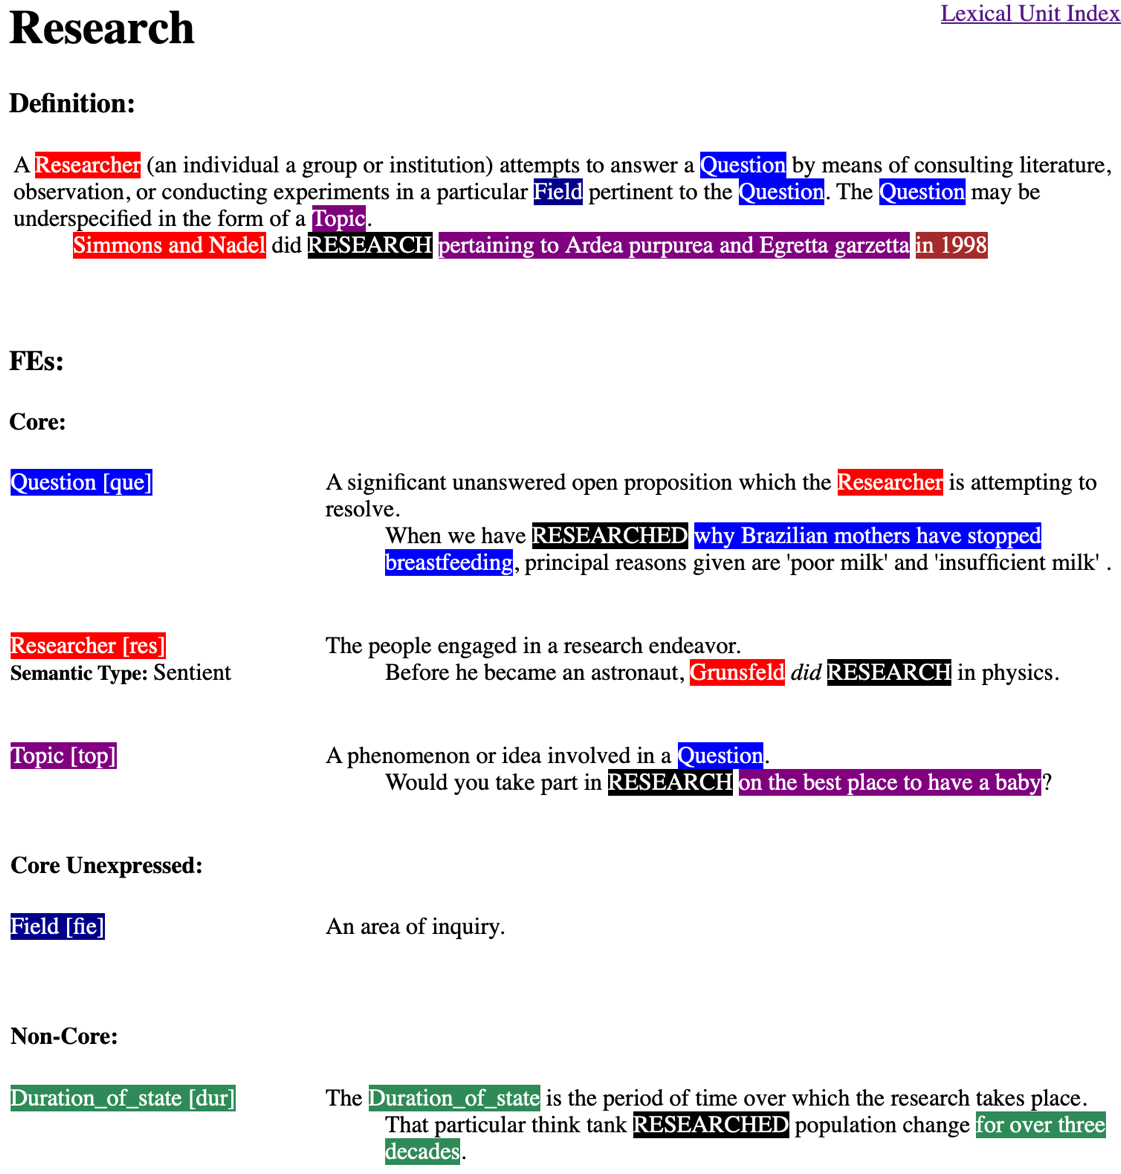
\includegraphics[width=\textwidth]{figures/media/image2.png}
  \caption{\label{fig:framenet-research}Ausschnitt aus dem \FN{Research}-Frame im Berkeley \emph{FrameNet} (Definition und ein Teil der FE).}
\end{figure}

Ersichtlich ist, dass der Frame aus den Kern-FE \textsc{question}, \textsc{researcher}, \textsc{topic}, sowie dem \emph{Core Unexpressed}\footnote{Als \emph{Core Unexpressed} werden solche FE annotiert, die zwar zu den Core-FE zählen, jedoch in Nachkommen des Frames nicht mehr explizit realisiert werden \autocite[24-25]{ruppenhoferFrameNetIIExtended2016}.} FE \textsc{field} besteht. Als \emph{Non-Core}-FE werden des Weiteren \textsc{duration\_of\_state}, \textsc{manner}, \textsc{means}, \textsc{place}, \textsc{population}, \textsc{purpose}, \textsc{time} und \textsc{type} gelistet. Eine kurze Definition und i.d.R. ein Beispielsatz geben des Weiteren Auskunft über die Rolle, die die jeweiligen FE im Gesamt-Frame spielen. Deutlich wird an dieser Stelle die Orientierung der Fillmoreschen Frame-Semantik an der Valenzgrammatik. So entsprechen die \emph{Core}-FE i.d.R. den Komplementen bzw. Ergänzungen des Verbs und die \emph{Non-Core}-FE seinen Supplementen bzw. Angaben.\footnote{Findet sich für ein \emph{Core}-FE keine lexikalische Realisierung, wird dies als ‚Nullinstantiierung` annotiert \autocite[28]{ruppenhoferFrameNetIIExtended2016}.} Es wird für den Frame des Weiteren angegeben, dass sich die FE \textsc{field}, \textsc{question} und \textsc{topic} in einem FE-\emph{CoreSet} zusammenfassen lassen, von ihnen also i.d.R. nur eines realisiert wird \autocite[25-26]{ruppenhoferFrameNetIIExtended2016}. Als LE, d.\,h. frame-evozierende Lexeme, sind ihm \emph{investigate.v, research.n} und \emph{research.v} zugeordnet. Eine LE stellt dabei immer ein Wort-Frame-Paar dar, sodass im Falle polysemer oder homonymer Wörter ein Wort auch mehreren Frames zugeordnet sein kann, es also mehrere gleichlautende LE geben kann. Eine gewisse Disambiguierung leisten darüber hinaus die den LE angefügten \emph{Part-of-Speech}-Tags (POS-Tags), die \emph{research} in diesem Frame ein Mal als Nomen und ein Mal als Verb ausweisen. Im Frame-Eintrag sind außerdem Frame-zu-Frame-Relationen vermerkt; in diesem Fall, dass der Frame seine Struktur bzw. Semantik vom \FN{Scrutiny}-Frame erbt und wiederum an den \FN{Trying\_out}-Frame vererbt. Die Idee ist dabei, dass „each semantic fact about the parent must correspond to an equally specific or more specific fact about the child'' \autocite[80]{ruppenhoferFrameNetIIExtended2016}. In diesem Sinne lassen sich teils übereinstimmende FE identifizieren, auch wenn die FE des Kind-Frames häufig semantisch differenzierter sind. Weiterhin wird der \FN{Cogitation}-Frame unter „Uses:`` angegeben, was einer „reference in a very general kind of way to the structure of a more abstract, schematic frame`` entspricht und insbesondere für Fälle genutzt werden soll, in denen ein Teil der durch den Kind-Frame aufgerufenen Szene auf den Eltern-Frame Bezug nimmt \autocite[83]{ruppenhoferFrameNetIIExtended2016}. \figref{fig:framegrapher-research} zeigt die für Frames typische Visualisierung der Vernetzung des Frames in \emph{FrameNet} als Netzwerk-Graph:

\begin{figure}
  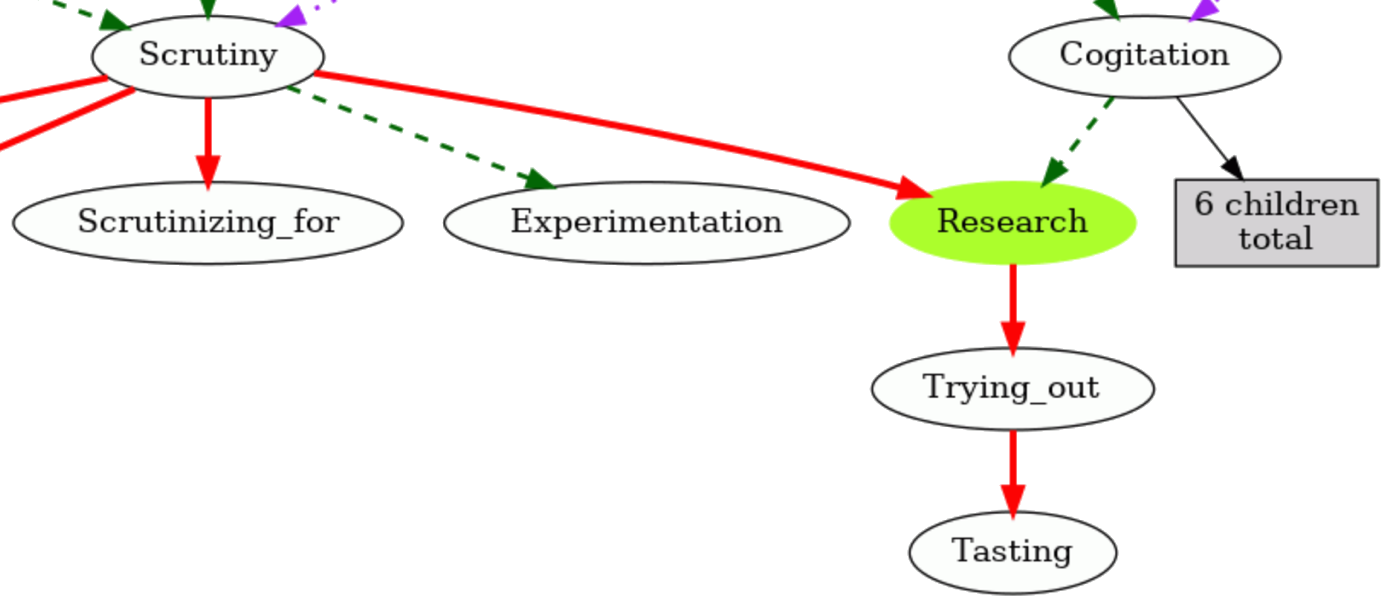
\includegraphics[width=\textwidth]{figures/media/image3.png}
  \caption{\label{fig:framegrapher-research}Ergebnis der Abfrage des \FN{Research}-Frames im \emph{FrameGrapher}-Tool in \emph{FrameNet} (\emph{maximum number of generations}: 2, \emph{maximum number of peripheral children}: 5).}
\end{figure}

\subsubsubsection{Erstellungsprozess eines Frame-Eintrags}\label{erstellungsprozess-eines-frame-eintrags}

Die Erstellung eines \emph{FrameNet}-Frames lässt sich wie folgt gliedern: Ausgangspunkt ist der Eindruck der Annotator*innen, dass einer Gruppe von Wörtern ein oder mehrere gemeinsame Frames unterliegen könnte. Dieser Eindruck wird sodann anhand von Korpusevidenz näher geprüft und es werden aus den LE ein oder mehrere Frames erstellt \autocite[11]{ruppenhoferFrameNetIIExtended2016}. Als Anforderung für den gemeinsamen semantischen Nenner von Wörtern können dabei die folgenden, den situativ-szenischen Charakter von Frames addressierenden Kriterien gelten: „a background of the kinds of questions they answer, the kinds of situations that are presupposed for sentences with the target, and the way that a speaker is thinking about a situation when they use the target'' \autocite[11]{ruppenhoferFrameNetIIExtended2016}. Sie sollen darüber hinaus insbesondere die gleiche Anzahl und Art von FE aufweisen.\footnote{An dieser Anforderung wird noch einmal deutlich, dass \emph{FrameNet}-Frames sehr eng an valenztheoretischen Ideen ausgerichtet ist, denn scheinbar lassen sich FE schon unabhängig von Frames für einzelne Wörter bestimmen.} Welche Methoden bei der Sammlung von LE, die zu einem Frame gehören, zum Einsatz kommen, bzw. ob dabei überhaupt ein systematisches methodisches Vorgehen angewandt wird, bleibt allerdings offen.

\subsubsubsection{Welche Frames werden aufgenommen?}\label{welche-frames-werden-aufgenommen}

\emph{FrameNet} ist insgesamt eher einem lexikographischen Zugang verpflichtet als einem, der ein wirklich breites semantisches Wissen, wie Fillmore es noch in der \emph{Understanding-Semantics}-Phase gefordert hatte, oder gar das ‚gesamte verstehensrelevante Wissen` im Sinne Busses einbeziehen würde. Selbst die Ebene des namensgebenden Frames rückt zugunsten der angezielten lexikalischen Ebene eher in den Hintergrund, wenn es in der Dokumentation zum Berkeley-\emph{FrameNet} heißt:

\begin{quote}
The Berkeley FrameNet project is creating an on-line lexical resource for English, based on \textbf{frame semantics} and supported by corpus evidence. The aim is to document the range of semantic and syntactic combinatory possibilities-- \textbf{valences}--of each word in each of its senses, through computer-assisted annotation of example sentences and automatic tabulation and display of the annotation results. \autocite[7]{ruppenhoferFrameNetIIExtended2016}
\end{quote}

Durch die Ausrichtung des Projektes auf Wortvalenzen ist außerdem ein recht starker Fokus auf Verben und deverbale Nominalisierungen zu konstatieren, was bereits durch Fillmore so angedacht ist. Dies hängt auch mit dem Konzept des „dominant frame`` \autocite[324]{fillmoreFramenetActionCase2003} zusammen, das die Autor*innen einführen, jedoch kaum näher erläutern. Nur in Ausnahmefällen, etwa bei Funktionsverbgefügen („support expressions``), könne ein Nomen den dominanten Frame eines Satzes evozieren:

\begin{quote}
Although in principle members of all major lexical categories can evoke a semantic frame, the dominant semantic frame of a sentence is usually evoked by the sentence's main verb. In some situations, however, it is a noun that provides the dominant frame; in fact, in certain styles of academic or political writing the dominant frame informing the meaning of the sentence is a noun \autocite[324]{fillmoreFramenetActionCase2003}.
\end{quote}

Auch in den aktuellen \emph{FrameNet}-Guidelines wird dies deutlich. Zwar wird Nomen generell ein Frame-evozierendes Potenzial zuerkannt, dieses sei bei Nomen, die Ereignisse oder Beziehungen bezeichnen, jedoch wesentlich ausgeprägter als etwa bei solchen, die Artefakte benennen \autocite[43]{ruppenhoferFrameNetIIExtended2016}. Dieser Maßgabe folgend, ist die Annotation von Frames an Nomen, die etwa Artefakte bezeichnen, noch immer die Ausnahme in \emph{FrameNet}. Ihnen wird zwar eine „minimal frame structure of their own`` \autocite[8]{ruppenhoferFrameNetIIExtended2016} zugesprochen, sie sollten jedoch vornehmlich als FE annotiert werden. Die Autor*innen gehen sogar so weit, dass die Annotation von Artefakt-bezeichnenden Nomen nur ein Mittel sein könne, um die Verben auffindbar zu machen, die diese Sätzen eigentlich regieren \autocite[8, siehe auch 51-52]{ruppenhoferFrameNetIIExtended2016}.

Neben der wortartbasierten Auswahl von Frames stellt auch die Frage der Granularität einen Aspekt dar, der über die in \emph{FrameNet} enthaltenen Frames entscheidet. Er ist für eine Frame-lexikographische Ressource von überragender Wichtigkeit; Ruppenhofer et al. \autocite*[17]{ruppenhoferFrameNetIIExtended2016} bezeichnen ihn sogar als „the most fundamental question``. Dass es etwa keine unterschiedlichen Frames für ‚Essen` und ‚Trinken` gibt, die in der Frame-Hierarchie dem bereits vorhandenen \FN{Ingestion}-Frame untergeordnet sein könnten, begründen sie mit forschungspraktischen Limitationen \autocite[17]{ruppenhoferFrameNetIIExtended2016}. Insgesamt wird dieser zentrale Aspekt jedoch nur sehr kurz thematisiert und wirkt unterreflektiert -- insbesondere vor dem Hintergrund der bereits thematisierten scheinbar wenig systematischen Auswahl zu beschreibender Frames durch das Annotationsteam. Die tatsächliche Frame-Auswahl kann diesen Eindruck nicht völlig entkräften. Einerseits finden sich Frames, die auf relativ spezifische Situationen eingehen wie der \FN{Bail\_decision}-, der \FN{Knot\_creation\_scenario}- oder der \FN{Hunting\_success\_or\_-failure}-Frame. Andererseits sind geradezu fundamentale soziale Konzepte, ohne die eine Orientierung in gesellschaftlichen Diskursen der vergangenen Jahre kaum möglich ist, wie ‚Krieg`, ‚Frieden`, ‚Pandemie` oder eben ‚Extremismus` nicht enthalten. Eine mögliche Lösung wäre es hier, auf semantisch ähnliche Frames wie \FN{Terrorism} statt ‚Extremismus` oder \FN{Hostile\_encounter} statt ‚Krieg` zurückzugreifen. Alternativ könnten auch semantisch sehr vage Frames wie der \FN{Catastrophe}-Frame, der als „\textsc{undesirable\_event} which affects the \textsc{patient} negatively``\footnote{\url{https://framenet.icsi.berkeley.edu/frameIndex}} definiert ist, genutzt werden. Als weitere Strategie zum Umgang mit diesem Problem wird die Definition neuer, an \emph{FrameNet} orientierter Frames vorgeschlagen und praktiziert \autocites[etwa bei][]{scholzVokabularImDiskurshistorischen2015, dutraBuildingFrameSemanticModel2023, bisiadaMeTooDreiSprachen2023}.

\subsection{Das Frame-Konzept Dietrich Busses}\label{das-frame-konzept-dietrich-busses}

\subsubsection{Überblick}\label{ueberblick}

In diesem Kapitel möchte ich das von Dietrich Busse im Rahmen seines Kompendiums zur Frame-Semantik \autocite*{busseFrameSemantikKompendium2012} entwickelte Frame-semantische Arbeitsmodell vorstellen. Das Modell kann als eine Zusammenführung und Erweiterung verschiedener Slot-Filler-Frame-Modelle begriffen werden. Besonderen Einfluss haben dabei die Arbeiten Bartletts, Fillmores, Minskys, Schank und Abelsons, Barsalous sowie die einiger germanistischer Linguist*innen, darunter Konerding, Lönneker-Rodman, Klein und Ziem. Das folgende Zitat fasst Status, Wesen und Funktion von Frames im Sinne Busses zusammen:

\begin{quote}
Ein Frame bezieht sich auf ein „Etwas``, das erst durch die „Attribute`` des Frames, denen jeweils bestimmte „Werte`` zugewiesen werden müssen, als dieses Etwas bestimmt, d.\,h. als ein aus dem Kontinuum der zunächst ungeschiedenen Sinnesdaten heraushebbares „Etwas`` ausgegrenzt wird. D.\,h.: Erst dadurch, dass ihm Eigenschaften (via Attribute) zugeschrieben werden, wird es als etwas Identisches kognitiv bzw. epistemisch „greifbar``, bekommt eine Identität, die es überhaupt erst zu einem wiederholt referierbaren „Etwas`` machen. Die „Kategorie`` in Barsalous Sinne (die dann im Sinne Lönnekers mit einem „Frame-Namen`` benannt wird) ist also zunächst nichts anders als eine abstrakte (epistemisch „leere``) Position im Sinne eines „hier gibt es ein Etwas``. Erst durch die Spezifikation von konkreten Merkmalen, Eigenschaften, die dieses „Etwas`` von anderen „Etwassen`` abzugrenzen erlauben, im Sinne der Attribute Barsalous, bekommt dieses „Etwas`` eine konkrete, mit Informationen gefüllte, und auch erst dann wiedererkennbare Gestalt. „Wiedererkennbar`` meint dann, dass mit dem „Datenset``, der den Frame ausmacht, neue Wahrnehmungssituationen (oder epistemische Konfigurationen) kognitiv verarbeitet werden, so dass sie als „Exemplare`` des Frames identifiziert werden können. Ein „allgemeiner`` Frame ist dann so etwas wie eine Datenstruktur, gemeint als abstrakte „Suchstruktur``, die im kognitiven (epistemischen) Prozess der Identifizierung von Entitäten (als Entitäten eines bestimmten Typs) angewendet wird. Die konkrete Datenstruktur im Kontinuum der Sinnesdaten bzw. kognitiven Konfigurationen, die durch die Aufprägung der abstrakten Struktur ausgegrenzt wird, ist dann ein „Exemplar`` dieses Frames. \autocite[589]{busseFrameSemantikKompendium2012}
\end{quote}

In diesem Zitat werden mehrere Wesensmerkmale von Frames im Sinne Busses deutlich:

\begin{enumerate}
\def\labelenumi{\arabic{enumi})}
\item
  Frames sind epistemische Entitäten, die es ermöglichen, eingehende „Sinnesdaten`` zu verarbeiten und in dem Sinne zu ordnen, dass sie als etwas Zusammengehöriges wahrgenommen werden, ihnen eine „Identität`` zugeschrieben wird und sie somit als „Etwas`` erkennbar sind. Die Wiedererkennbarkeit und der epistemische Gehalt wird durch die Zuschreibung von Eigenschaften über Attribute geleistet; die Referenzierbarkeit über einen Frame-Namen. Es wird hier auch der konstruktivistische Charakter von Frames deutlich: Gegenstände werden erst in der Verarbeitung von Eindrücken konstituiert und sind nicht einfach ‚da`.
\item
  In diesen Verarbeitungsprozessen geht es insbesondere um die musterbasierte Wiedererkenneung bzw. Identifizierung von Frames. Sie finden ausdrücklich auf einer kognitiven Ebene statt. Auf die Rolle dieser mit dem Frame-Konzept verbundenen und nicht unumstrittenen Festlegung wird in \chapref{frames-und-kognition} noch näher eingegangen.
\item
  Es werden zudem verschiedene Ebenen oder Zustände von Frames beschrieben. Zu unterscheiden ist dabei u.\,a. zwischen den kognitiven, schablonenartigen Datenstrukturen, die zur Einordnung von Sinnesdaten herangezogen werden und den Daten selbst, die mithilfe dieser Struktur als passend zur Schablone identifiziert werden. Mit diesem Aspekt wird sich das folgende Kapitel auseinandersetzen.
\end{enumerate}

\subsubsection{Type- und Token-Frames}\label{type--und-token-frames}

Busse bleibt nicht bei dieser Beschreibung verschiedener eher prozesshafter Frame-Zustände, sondern differenziert Frames nach insgesamt fünf (hier nicht im Detail aufgeführten) Ebenen und mithilfe der folgenden drei Kriterien: dem Muster- bzw. Exemplarcharakter der Frames (Type- vs. Token-Frames), der Art von Wissen, die sie organisieren (soziales vs. individuelles Wissen) und ihrem kognitiven Status bei der Wissensrealisierung (allgemeine Frames vs. konkret im individuellen Kurzzeitgedächtnis instantiierte Frames). Besonders relevant und von Busse immer wieder hervorgehoben ist die Unterscheidung von Type- und Token-Frames, verstanden als „die Differenz zwischen einem abstrakten Muster und seiner konkreten Anwendung / Realisierung / Konkretisierung / Aktualisierung`` \autocite*[614]{busseFrameSemantikKompendium2012}. Unter einem Type-Frame ist also ein schablonenhafter Frame zu verstehen, dessen Slots offen oder nur mit Default-Werten befüllt sind und der als bestehendes Muster dazu dient, Sinneseindrücke einzuordnen. Token-Frames hingegen sind Realisierungen der Type-Frames und insofern mit konkreten Daten gefüllt und entsprechend darzustellen \autocite[539]{busseFrameSemantikKompendium2012}.

Es lassen sich des Weiteren Frames des individuellen kognitiven Wissens von solchen des sozialen Wissens unterscheiden. Für die spätere Operationalisierung und Methodenentwicklung ist relevant, dass die individuellen, kognitiven Frames nicht unmittelbar zugänglich sind, sondern nur interpretativ „auf der Grundlage von sprachlichen, ko-textuellen, kontextuellen und situativen Daten sowie ‚Hintergrundwissen`\,`` \autocite[538]{busseFrameSemantikKompendium2012} rekonstruiert werden können. In Hinblick auf die Erschließbarkeit von Token- und Type-Frames ist davon auszugehen, dass die Instantiierung von Token-Frames in einer konstitutiven Wechselwirkung mit den musterhaften Type-Frames steht, letztere mithin in einem Abstraktionsschritt aus der Menge der rekonstruierten Token-Frames ermittelt werden können. Aufgrund der Rekursivität von Frames ist allerdings davon auszugehen, dass „solche Beschreibungen eher komplexen Frame-Vernetzungen als isolierten Einzel-Frames entsprechen`` \autocite[538]{busseFrameSemantikKompendium2012}.

\subsubsection{Frame-Struktur: Slots, Filler und Relationen}\label{frame-struktur-slots-filler-und-relationen}

Wie Fillmore, Minsky und Barsalou entwirft auch Busse ein Frame-Modell, das aus einem Frame-Kern und einer Slot-Filler-Struktur besteht, wobei der Frame-Kern eher eine benennende als eine epistemisch spezifizierende Funktion hat, indem er „markiert, dass es hier ein (epistemisches) ‚Etwas` gibt, auf das sich die nachfolgend spezifizierten Frame-Elemente, Relationen und Aspekte beziehen`` \autocite[731]{busseFrameSemantikKompendium2012}. Die Filler der Slots stellen jeweils selbst Frames dar, sodass man, wie auch bei Minsky und dann insbesondere bei Barsalou,\footnote{So heißt es bei Barsalou „Knowledge appears to be frames all the way down, with every component of a frame potentially decomposing recursively into a more specific frame.`` \autocite*[41]{barsalouFlexibilityStructureLinguistic1993}} von einem rekursiven Frame-Modell sprechen kann, das im Folgenden anhand einer Abbildung Busses (\figref{fig:maus-frame}) näher erläutert werden soll:

\begin{figure}
  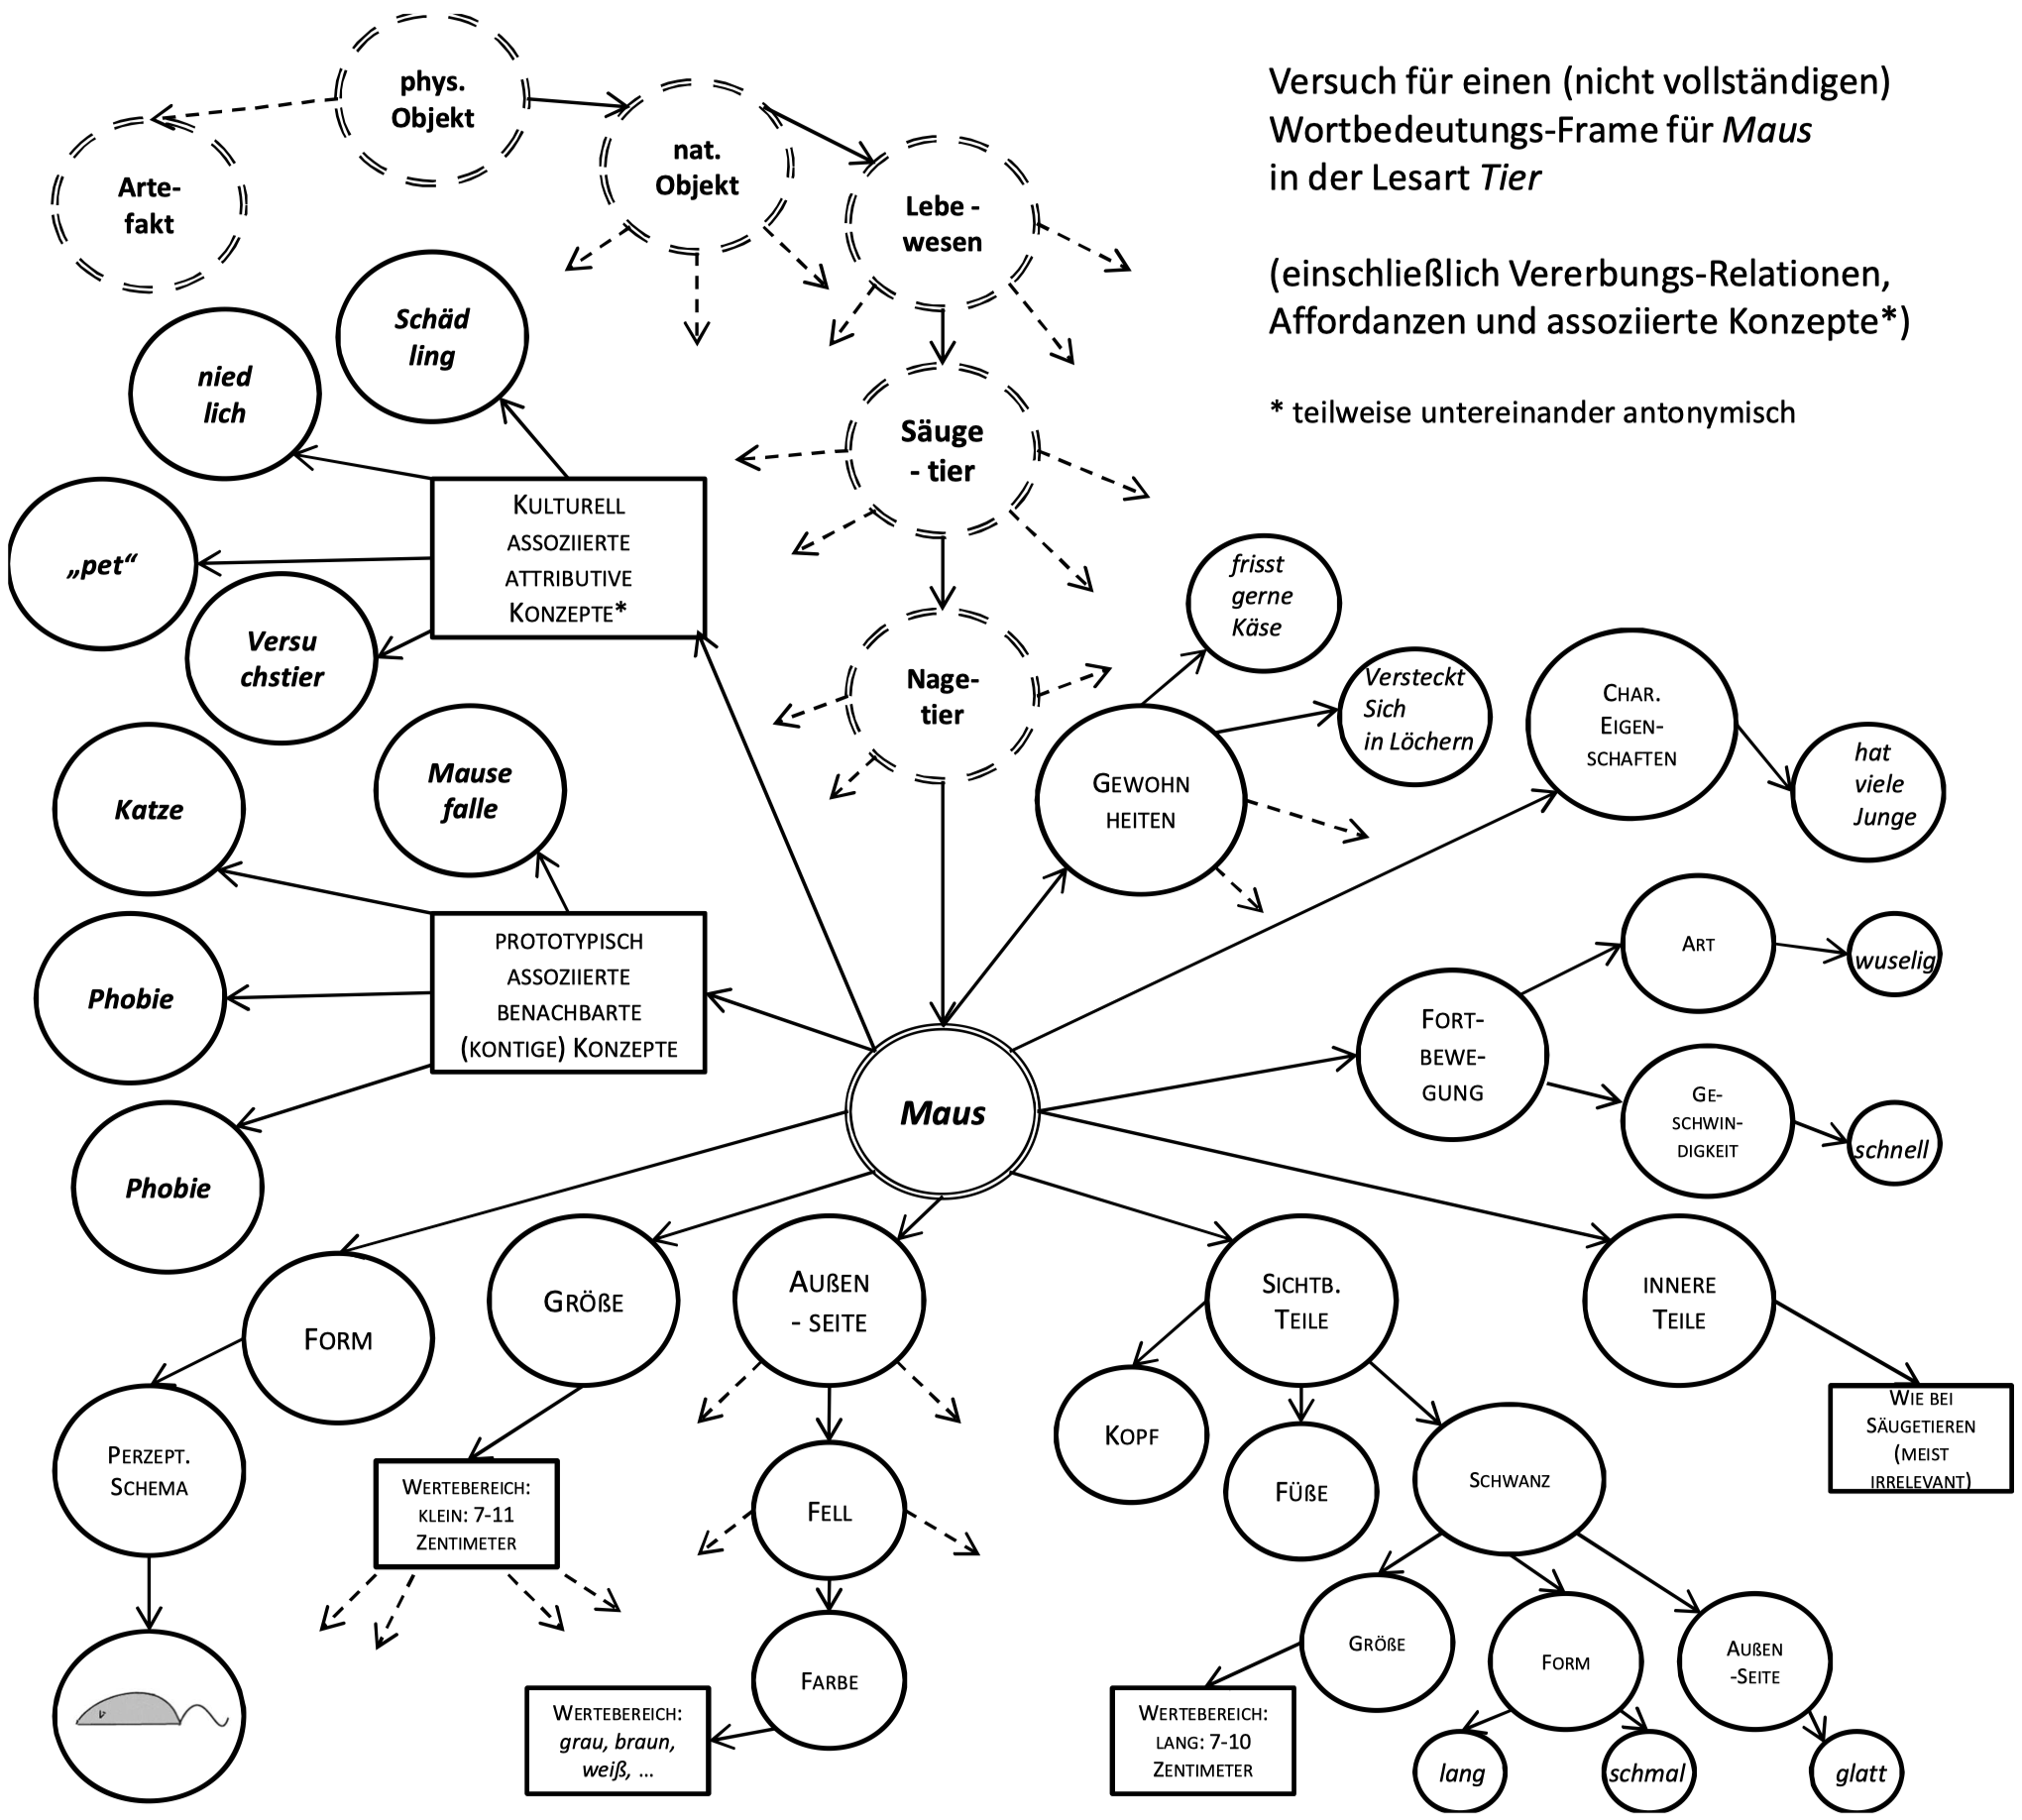
\includegraphics[width=\textwidth]{figures/media/image4.png}
  \caption{\label{fig:maus-frame}Entwurf eines Maus-Type-Frames (Abbildung 7-30 aus \citealt[744]{busseFrameSemantikKompendium2012}).}
\end{figure}

Es wird zunächst deutlich, dass der Maus-Frame selbst von einer Reihe übergeordneter Frames abstammt (Artefakt → phys. Objekt → nat. Objekt → Lebewesen → Säugetier → Nagetier). Slots und Filler sind in der Abbildung als Knoten angezeigt, während die Relationen zwischen ihnen als gerichtete Kanten (Pfeile) abgebildet werden. Alternative Relationen sind jeweils als gestrichelte, feste Relationen als durchgehende Pfeile dargestellt. Einzelne Werte sind nur in den Blättern des Baumes zu finden und durch einen den Text eng umschließenden Kreis verwirklicht. Werden keine konkreten Werte, sondern Wertebereiche angegeben, so geschieht dies in Form eines Vierecks. Während bei Token-Frames auch auf der untersten dargestellten Ebene die Filler der Slots angegeben werden, werden beim hier dargestellten Type-Frame Wertebereiche notiert, in denen sich die Filler typischerweise bewegen sowie der Typ des Wertebereichs und ggf. eine Information dazu, inwiefern eine konkrete Füllung des Slots oder ein Default-Wert\footnote{Das Konzept des Default-Wertes -- dass also nicht jedes Wissenselement sprachlich explizit gemacht werden muss und dennoch als mit einem bestimmten Wert belegt mitverstanden wird -- gibt es bereits bei Minsky; es wird aber insbesondere von Ziem \autocite*{ziemFramesUndSprachliches2008} als für die Frame-Semantik zentral herausgestellt. Er bezeichnet sie auch als „{[}i{]}mplizite Prädikationen``, die seines Erachtens den „weitaus größt{[}en{]} Teil verstehensrelevanten Wissens`` in Texten ausmachen \autocite[335]{ziemFramesUndSprachliches2008}} zu erwarten ist \autocite[731-732]{busseFrameSemantikKompendium2012}. So wird etwa für den Slot ‚Farbe` der offene Wertebereich „grau, braun, weiß, ...`` angegeben. Auch assoziative attributive und benachbarte Konzepte werden -- ebenfalls durch ein Viereck gruppiert -- in die Frame-Darstellung aufgenommen und ergänzen in diesem Beispiel die ansonsten weitestgehend enzyklopädischen Daten durch eher kulturbezogene Aspekte.

Busse beschreibt darüber hinaus Relationen zwischen Frame-Elementen, die nicht auf Vererbungs- bzw. Slot-Filler-Relationen zurückgehen, sondern das gemeinsame Auftreten von Frame-Elementen steuern:

\begin{quote}
In Frames bestehen zusätzlich zu den Typen von Relationen, die Anschlussstellen (Slots, Attribute) den Frame-Kernen, sowie Zuschreibungen (Filler, Werte) den Anschlussstellen (den jeweiligen Slots) zuordnen, weitere zentrale, teilweise ebenfalls Frame-definierende Typen von Relationen, die einzelne Frame-Elemente (Anschlussstellen / Slots / Attribute und / oder Zuschreibungen / Filler / Werte) untereinander korrelieren, sie zu Frame-spezifischen Gruppen von Frame-Elementen zusammenfassen, die immer gemeinsam vorkommen müssen, oder sachlich zwingende Kovarianzen (bzw. Abhängigkeits-Relationen) zwischen einzelnen Zuschreibungen (Fillern, Werten) festlegen. Diese Relationen (Korrelationen, Kovarianzen) wirken als die Variabilität der Frame-Struktur einschränkende Bedingungen (Restriktionen, Beschränkungen), die entweder bestimmte Frame-Elemente (beim Auftreten anderer korrelierter Frame-Elemente) erzwingen (konstruktive Korrelationen), oder das Auftreten bestimmter Frame-Elemente (z.\,B. Filler, Werte) zu bestimmten Anschlussstellen in Kovarianz mit bestimmten anderen Frame-Elementen (Fillern, Werten) zu bestimmten anderen Anschlussstellen auf einen bestimmten Bereich beschränken (restriktive Korrelationen). \autocite[570-571]{busseFrameSemantikKompendium2012}
\end{quote}
\largerpage
Er untergliedert diese „\emph{Relationen zwischen Attributen gleichen Typs}`` in ‚Gruppen von Attributen`, ‚Strukturelle Invarianten` und ‚Attribut-Constraints`. Erstere können entweder statistisch-usuell bestimmt werden als „bestimmte festere Ko-Okkurenzen von Slots bzw. Attributen`` oder als „inhaltlich spezifizierte und zusammenhängende Gruppen (die sich dann nur enzyklopädisch beschreiben / definieren bzw. abgrenzen lassen)`` \autocite[594]{busseFrameSemantikKompendium2012}, womit etwa die auf das Aussehen der Maus bezogenen FE wie \textsc{Form}, \textsc{Größe} oder \textsc{Außenseite} gruppiert werden könnten. Darüber hinaus sei auch eine funktionale Bestimmung der Attributgruppen möglich, etwa nach (vor allem bei verbal geprägten Frames relevanten) Aktanten- und (vor allem bei nominal geprägten Frames relevanten) Eigenschafts-FE. Den Begriff der ‚strukturellen Invariante` übernimmt Busse von Barsalou, der damit feste, notwendige Beziehungen zwischen FE bezeichnet, die etwa räumlicher oder zeitlicher Natur sein können. Als Beispiel für erstere nennt Busse die Relation zwischen Sitz und Lehne bei einem Stuhl, für zweitere die Relation zwischen Essen und Bezahlen \autocite*[565]{busseFrameSemantikKompendium2012}. Auch in Bezug auf Wertebereiche spielen strukturelle Invarianten eine Rolle, indem sie für bestimmte Wertebereiche eine quasi absolute Grenze setzen, bei deren Überschreitung nicht mehr von einer Extension des Wertebereiches um einen vielleicht ungewöhnlichen Wert ausgegangen werden kann. Der Begriff \emph{constraint} letztlich wird ebenfalls von Barsalou übernommen. Hiermit sind Wechselwirkungen zwischen den FE gemeint, die anders als bei den strukturellen Invarianten nicht als „normativ{[}e{]} Wahrheiten`` zu fassen sind, sondern eher eine „‚systematische Variabilität` zwischen den Werten von Attributen {[}herstellen{]}`` und darüber hinaus häufig auf Alltagswissen beruhen \autocite[566]{busseFrameSemantikKompendium2012}. Als Beispiele führt Busse an, dass ‚Mallorca` als Filler für den Slot \textsc{Ort} in einem Urlaub-Frame bestimmte Filler für den Slot \textsc{Urlaubsaktivität} nahelegt (etwa ‚surfen`), während andere Filler wie ‚skifahren` nur bei anderen Urlaubsorten zu erwarten sind. Solche Constraints können sowohl zwischen Slots als auch Fillern auftreten.

\subsubsection{Sprachoberflächliche Bezugspunkte}\label{sprachoberflaechliche-bezugspunkte}
\largerpage
Für eine diskurslinguistische Arbeit sind Frames als Strukturen epistemischen Wissens insbesondere unter Berücksichtigung ihrer sprachlichen Repräsentation von Interesse. Es geht also darum, wie von Texten überhaupt auf Frames geschlossen werden kann oder auch wie Frames Texte und Texte Frames formen. Die Frame-Theoretiker entwerfen dieses Verhältnis jeweils unterschiedlich, wobei die lexikalische Ebene i.d.R. den primären Bezugspunkt darstellt. Für Busse stellt die „adäquate Analyse der Beziehungen zwischen Lexemen und Frames`` die „wichtigste Aufgabe einer angewandten Frame-Forschung`` dar, wobei er seine eigenen Ausführungen als „erste tastende Vermutungen``, die weiterer Forschung und empirischer Validierung bedürfen, einordnet \autocite*[656]{busseFrameSemantikKompendium2012}. Im Folgenden möchte ich die in meinen Augen wichtigsten Aspekte seiner Überlegungen zusammenfassen, die vollständige Darstellung findet sich in Busse \autocite*[652-658 insb.]{busseFrameSemantikKompendium2012}

Als Frame-evozierendes sprachliches Zeichen stellt auch er das Lexem in den Fokus. Lexeme evozieren Frames und legen -- unter Umständen im Zusammenspiel mit anderen Lexemen des Kotextes -- Slots und Filler von Frames sowie eine bestimmte Perspektive fest \autocite[656-657]{busseFrameSemantikKompendium2012}. Die Zuordnung von Lexemen zu Frames ist dabei jedoch nie starr; stattdessen hebt Busse Minskys Idee eines probabilistischen \emph{matching process} hervor:

\begin{quote}
Laut Minsky gleicht das Wort-Verstehen eher einem Abgleich-Prozess (matching process), bei dem möglicherweise mehrere Frames durchlaufen werden, bevor der passende aktiviert und herausgefunden ist. Verstehen von Wörtern wird damit zu einem \emph{probabilistischen} Unterfangen, das auf Plausibilitäten und Wahrscheinlichkeiten eher beruht als auf eindeutigen Gewissheiten. \autocite[653]{busseFrameSemantikKompendium2012}
\end{quote}

Dazu passt auch, dass Lexeme in Busses Frame-Entwurf „mehr als einen Frame parallel evozieren`` oder mehrere Lexeme den gleichen Frame evozieren können \autocite[657]{busseFrameSemantikKompendium2012}. Höchst interessant für die vorliegende Arbeit ist, dass er die Bedeutung wesentlicher kontextualistischer Konzepte hervorhebt, die insbesondere im Rahmen korpuslinguistischer Theoriebildung eine herausragende Rolle gespielt haben (siehe \chapref{distributionelle-semantik-korpuspragmatik-und-das-corpus-driven-paradigma}). Dazu zählt insbesondere die Kontextualisierungsleistung von Kollokationen, die für ihn darin besteht, andere Frames anzuschließen und einen Frame mithin semantisch zu spezifizieren: „Lexeme kontextualisieren Frames, indem sie sie in Kollokationen und Syntagmen einbetten und dadurch Beziehungen zu anderen Frames nahelegen.`` \autocite[656]{busseFrameSemantikKompendium2012}. Busse konstatiert zur Bedeutung von Kollokationen des Weiteren einen Zusammenhang, den bereits Minsky hervorgehoben hat, nämlich dass Frames mitunter nicht durch ein einzelnes Lexem, sondern durch das Zusammenspiel verschiedener Lexeme evoziert werden. So zitiert Minsky ein Beispiel aus Charniak \autocite*{charniakModelChildrensStory1972}, in dem das Szenario beschrieben wird, dass ein Kind einem anderen einen Drachen schenken möchte, jedoch nicht das nötige Geld dafür hat:

\begin{quote}
She wondered if he would like a kite. She went to her room and shook her piggy bank. It made no sound. \autocite[Charniak 1972 in][35]{minskyFrameworkRepresentingKnowledge1974}
\end{quote}

Obwohl in dem Szenario nicht explizit von (keinem) Geld, einem Kind oder einem Geschenk die Rede ist, werden die entsprechenden Frames durch die syntagmatische Kombination der einzelnen Wörter evoziert. Es wird also deutlich -- und das ist für einen korpuslinguistischen Zugang von höchstem Interesse -- dass auch syntagmatische Lexemkombinationen, korpuslinguistisch gesprochen: Kollokationen, für die Frame-Evokation von Bedeutung sind. Sie evozieren zum einen mehrere für das Verständnis relevante Frames, zum anderen sorgen sie dafür, dass die einzelnen Frames zueinander kompatibel ausgewählt werden:

\begin{quote}
Lexem-Kombinationen und Lexem-Ketten evozieren Frame-theoretisch gesehen einerseits Kombinationen von Frames, andererseits führt die Kombination von Lexemen dazu, dass in einem Abgleich-Prozess (matching process im Sinne von Minsky) die ausdrucksseitige Präsenz von zwei oder mehreren Lexemen die Evokation der Lexem-induzierten Frames wechselseitig adaptiv beeinflusst, genauer: die evozierten Frames an den durch die Kombination signalisierten epistemischen Kontext anpasst und ggf. irrtümliche erste (durch isolierte Lexem-Verarbeitung induzierte) Frame-Evokationen korrigiert. \autocite[660]{busseFrameSemantikKompendium2012}
\end{quote}

Ein weiteres Konzept, das der Korpuslinguistik entstammt und das Busse für relevant für die Beschreibung hält, ist das der semantischen Prosodie. Er referiert hier auf die Arbeiten der Korpuslinguisten Louw \autocite*{louwIronyTextInsincerity1993} und Stubbs \autocite*{stubbsTextCorpusAnalysis1996},\footnote{Wie Louw \autocite*[31-32]{louwIronyTextInsincerity1993} hervorhebt, geht der Begriff allerdings ursprünglich auf John Sinclair zurück.} die das Phänomen beschreiben, dass

\begin{quote}
lexikalische Wahlen oft starke Erwartungen dessen „was als nächstes kommt`` wecken. Es handelt sich bei diesem bisher kaum beschriebenen Phänomen um typische Kollokationen von Bezugswörtern mit anderen Wörtern, denen insgesamt eine semantische Tendenz der Verwendung der Bezugswörter zugrunde liegt mit dem Effekt, dass, wenn immer das Bezugswort verwendet wird, nur bestimmte Kollokate (mit einer bestimmten semantischen Tendenz) erwartet werden, auch wenn andere logisch genau so möglich wären. M.a.W., es geht um die „Präferenz`` von Lexemen, „sich mit einer ganzen semantischen Klasse von verbundenen Wörtern zu verbinden``, die dann ebenfalls wieder Frames und epistemische Kontexte evozieren. \autocite[655]{busseFrameSemantikKompendium2012}\footnote{Was Busse hier in Hinblick auf semantische Prosodie, also die semantische Färbung von Kollokaten, anspricht, ist nur ein Teilphänomen der von Sinclair beschriebenen Prinzipien der \emph{co-selection} bzw. des \emph{idiom principles} (siehe \chapref{der-corpus-driven-ansatz}), die für die Frame-semantische Modellierung genauso zu berücksichtigen wären.}
\end{quote}

Es ist also zu konstatieren, dass (sprachliche) Kontexte einen ganz wesentlichen Beitrag dazu liefern, einzelne Lexeme verstehen zu können, bzw. diese oft überhaupt erst im Verbund verständlich sind. Busse führt dazu auch die Positionen von Ballmer und Klein an, die diesen Punkt aus jeweils unterschiedlichen Positionen verdeutlichen: Während Ballmer den Fokus auf die Funktion von Sprachzeichen bei der Textproduktion legt, d.\,h. wie sie genutzt werden können, um bestimmte Kontexte im Wissen der Rezipient*innen aufzurufen, hebt Klein hervor, dass sich die Bedeutung sprachlicher Zeichen überhaupt nur in Bezug auf bestimmte Kontexte beschreiben lasse.

\subsubsection{Perspektivierung, Kontext und Frame-Wandel}\label{perspektivierung-kontext-und-frame-wandel}

In Busses Frame-Modell kann die Perspektivierung und Fokussierung eines Frames entweder durch die „Aktivierung bestimmter Sub-Sets von Slots / Attributen aus der Gesamt-Menge von Slots / Attributen eines \emph{type}-Frames`` oder durch die „Füllung der Slots mit spezifischen (Sets von) Werten`` geschehen \autocite[622]{busseFrameSemantikKompendium2012}. Dabei sei -- so Busses Arbeitshypothese -- die erste Variante typischer für Konkreta, die zweite für Abstrakta. Weiterhin relevant ist dabei, dass die nicht im Fokus bzw. Ausschnitt der Perspektive liegenden Teile des Frames weiterhin im Frame enthalten sind und referenzierbar bleiben:

\begin{quote}
Solche Perspektivierungen ändern jedoch nichts daran, dass in jeder Evozierung stets „der gesamte Frame präsent`` ist, wenn auch nicht in allen seinen epistemischen Elementen thematisch (oder im Aufmerksamkeitsfokus), doch als „Hintergrund``, eben „Kontext``, immer in seiner Gesamtheit „gegenwärtig`` (im Sinne von perspektivierbar, unmittelbar thematisierbar). \autocite[664]{busseFrameSemantikKompendium2012}
\end{quote}

Bedingt wird die Perspektivierung eines Frames bei Busse durch Ziele und Interessen, die er im Anschluss an Fillmore sowie die anderen von ihm betrachteten Frame-Theoretiker Minsky, Schank{\slash}Abelson und Barsalou in das Gebiet seiner Frame-Semantik einschließt \autocite*[620-621]{busseFrameSemantikKompendium2012}. Für den Rahmen dieser Arbeit besonders relevant ist dabei die Rolle für den Frame-Wandel, die er der Perspektivierung und Fokussierung sowie den sie leitenden „Ziel{[}en{]}, Interessen, Intentionen (und Zweck{[}en{]} und Funktionen)`` \autocite*[622]{busseFrameSemantikKompendium2012} bzw. rezipientenseitigen Erwartungen zuschreibt. Sie könnten sich nämlich „kognitiv oder sozial verfestigen und zu neuen \emph{type}-Frames (im individuellen oder gesellschaftlichen Wissen)`` bzw. zu „epistemisch verfestigt{[}en{]} Kontextualisierungen`` \autocite*[622]{busseFrameSemantikKompendium2012} führen. Die Rolle sprachlicher Zeichen ist dabei, dass sie die Perspektivierung bzw. Fokussierung leisten und -- sofern sich diese verfestigt -- zu „so etwas wie \emph{gesellschaftlich typisierte}{[}n{]} \emph{Perspektivierungen} und \emph{Fokussierungen} im Wissen`` \autocite[623]{busseFrameSemantikKompendium2012} führen. Zur Verfestigung von Slots bzw. Default-Werten von Slots rekurriert Busse außerdem auf Ziem \autocite*{ziemFramesUndSprachliches2008}, der mit Type- und Token-Frequenz zwei Formen von Verfestigung unterscheidet: Um eine hohe Type-Frequenz handelt es sich bei der Instanziierung eines Slots mit einer Vielzahl unterschiedlicher Token, während die wiederholte Instanziierung mit demselben Token eine hohe Token-Frequenz darstellt und zur Etablierung des Tokens als Default-Wert führt \autocite[627]{busseFrameSemantikKompendium2012}.

Sowohl in den Ausführungen zur sprachoberflächlichen Verankerung von Frames als auch zu ihrer epistemischen Perspektivierung ist bereits angeklungen, dass Ko- und Kontexte essenzieller Bestandteil einer angemessenen Frame-Modellierung sind und Einfluss auf Frames sowie die korrespondierenden sprachlichen Mittel haben. Bei Busse \emph{sind} Frames einerseits (epistemische) Kontexte, insofern sie einzelne Wissenselemente in größere Strukturen einbetten und somit kontextualisieren; er bezeichnet sie auch als „das Strukturformat für die verstehensrelevanten Wissens-Kontexte`` \autocite[664]{busseFrameSemantikKompendium2012}. Andererseits stellen Frames auch \emph{Mittel} der Kontextualisierung dar, insofern sie mittels der Verwendung einzelner sprachlicher Zeichen evoziert und perspektiviert werden. Gerade wenn Busse formuliert, dass Sprachzeichen „Kontextualisierungen ‚steuern`, insofern sie häufig bestimmte Perspektiven auf einen Wissenskomplex evozieren, d.\,h. bestimmte Aspekte eines Frame-Gefüges in den Vordergrund der Aufmerksamkeit und Relevanz rücken, andere im Hintergrund belassen``, \autocite[664]{busseFrameSemantikKompendium2012} wird außerdem eine inhaltliche Nähe zum Entmanschen Framing-Konzept deutlich (siehe \chapref{framing-in-den-kommunikationswissenschaften-bei-entman}). Interessanterweise nimmt Busse analog zum kontextuellen, wissensstrukturellen Charakter von Frames auch einen Kontextcharakter für Relationen sprachlicher Zeichen an. So stellen auch sie Kontexte dar, da sie in syntagmatischen und paradigmatischen Beziehungen zueinander stehen, was „in seiner Wichtigkeit und Wirkung unterschätzt`` \autocite[87]{busseDiskurslinguistikAlsKontextualisierung2007} werde. Gerade dass diese „eigen-kategorial{[}en{]}`` Relationen auf der Ebene der Sprachzeichen aufs engste mit ihren „fremd- oder kreuz-kategorial{[}en{]}`` \autocite[87]{busseDiskurslinguistikAlsKontextualisierung2007} Pendants auf der kognitiven Ebene, d.\,h. Frames, korrespondieren, liegt im Kerninteresse der vorliegenden Arbeit.

Die vielfältigen Kontextualisierungsmöglichkeiten, die sprachliche Zeichen bzw. Frames bieten, sind auch eng mit Aspekten des Frame-Wandels zusammenzudenken. Dieser wird von Busse als kontinuierlicher Prozess konzeptualisiert, der auf den einzelnen Token-Frame Instanziierungen im Diskurs beruht. Dadurch, dass Sprachteilnehmende Frames in der alltäglichen Kommunikation verwenden, wenn sie Äußerungen rezipieren oder produzieren, dabei immer wieder andere Slots und Filler wählen bzw. einem Frame zuordnen, verändern sich auch die Type-Frames. Es findet so, durch individuelle Äußerungen und über den Diskurs vermittelt, ständig Frame-Wandel statt:

\begin{quote}
In der individuellen Frame-Aktivierung schlagen sich die wechselhaften Positionen, Interessen, Ziele, Einstellungen, Perspektivierungen, Fokussierungen, Kontextualisierungen nieder, die dann teilweise (soweit sie „verbalisiert`` bzw. aus den sprachlich realisierten Texten sichtbar und nachvollziehbar sind) im gesellschaftlichen Diskurs „kommuniziert`` werden mit der möglichen Folge des „Aushandelns`` neuer Konventionen bzw. Strukturen der allgemeinen gesellschaftlich akzeptierten Frames (als Teil des „kulturellen Gedächtnisses``). Hat sich ein solcher Prozess der sozialen Verbreitung und Etablierung veränderter Frames vollzogen, hat ein diachroner Frame-Wandel stattgefunden, der dann entsprechend auch im individuellen Wissen einen Niederschlag finden kann. \autocite[627]{busseFrameSemantikKompendium2012}
\end{quote}

Diesen kontinuierlichen Wandelprozess, bei dem Frames kaum jemals plötzlich neu entstehen, sondern auf Anpassungen vorheriger Frames beruhen, bezeichnet Busse an gleicher Stelle auch als „Frame-Emergenz``. Dass dies funktioniert und Frames auch in Wandelprozessen identifizierbar bleiben, liegt auch an ihrem prototypikalischen Charakter. Aufgrund der zahllosen unterschiedlichen inner- und außersprachlichen Kontexte, in denen auf Frames zurückgegriffen wird, ist die Zuordnung ohnehin nie eindeutig, sondern ein probabilistischer Abgleichprozess \autocite[624]{busseFrameSemantikKompendium2012}.

\subsubsection{Frames und Kognition}\label{frames-und-kognition}

Frames sind bei Busse dezidiert kognitive Einheiten, die zwar über Diskurse ausgehandelt und geformt werden, letztlich jedoch mental bei Individuen repräsentiert sind. Dies ist vollkommen kongruent mit den wichtigsten in seinem Frame-Begriff integrierten Frame-Modellen -- so waren etwa Minsky und Barsalou ja selbst Kognitionswissenschaftler. Busse wendet sich damit gegen häufig an Wittgenstein anschließende ‚anti-mentalistische` Überlegungen, wie sie prominent etwa von Wolfgang Teubert vorgetragen werden. In mehreren argumentativen Schlagabtauschen \autocites{teubertWirklichkeitDiskurses2013, busseDiskursSpracheGesellschaftliches2013, teubertDietrichBusseUnd2018, teubertImKopfOder2019}[siehe auch][]{ziemSprachbegabteMenschIst2018} führen die beiden eine Auseinandersetzung darüber, ob Wissen auf der Diskurs- oder auf der kognitiven Ebene zu finden sei. Die Position Teuberts und anderer Vertreter des anti-mentalistischen Paradigmas gründet dabei auf dem Postulat ‚Man kann nicht in die Köpfe schauen`: Da es mithilfe linguistischer Methodik nicht möglich sei, tatsächliche kognitive Wissensbestände von Individuen zu beschreiben, sollte dieser Versuch auch nicht unternommen werden. Stattdessen sollte der Formationsort dieses Wissens, der Diskurs, in den Blick genommen werden:

\begin{quote}
Zur Zeit der mentalen Verarbeitung befindet sich dieses ‚verstehensrelevante Wissen` natürlich in den Köpfen der Beteiligten. Doch aufsuchen können wir es dort nicht. Wir wissen auch nicht, welche mentalen Mechanismen zum Einsatz kommen, die zu den entsprechenden Schlussfolgerungen führen. Aber es gibt einen sehr viel einfacheren Weg. Wir können dieses Wissen da dingfest machen, von wo es in die Köpfe gelangt ist. Denn zuvor hat es sich nirgendwo anders als im Diskurs befunden. \autocite[90]{teubertWirklichkeitDiskurses2013}
\end{quote}

Dieser Vorwurf Teuberts, vor allem an ‚in den Köpfen` vorliegenden Wissensstrukturen und mithin „privat{[}em{]} Wissen`` \autocite[85]{teubertWirklichkeitDiskurses2013} interessiert zu sein, ist im Lichte der tatsächlich von Busse ausformulierten Theorie nur bedingt zutreffend. Zwar formuliert Busse für seine Frame-Semantik explizit, dass „das erste Zugriffsobjekt einer Frame-semantischen Analyse konkrete instantiierte Frames im Sinne einer kognitiven / epistemischen Aktualisierung im Geist eines Sprachteilhabers sein müssten`` \autocite[538]{busseFrameSemantikKompendium2012}. Schon im nächsten Satz heißt es jedoch:

\begin{quote}
Allerdings gibt es zu diesen keinen direkten Zugang und mit normalen linguistischen Methoden auch kein verlässliches Verfahren der Erschließung. „Instantiierte Frames`` in diesem Sinne können auf der Grundlage von sprachlichen, ko-textuellen, kontextuellen und situativen Daten sowie „Hintergrundwissen`` also allenfalls durch Rekonstruktion konstruiert werden. Diese Rekonstruktion trägt immer interpretative Züge. \autocite[538]{busseFrameSemantikKompendium2012}
\end{quote}

Das von Teubert beschriebene Problem ist also von Busse erkannt und reflektiert -- ein unmittelbarer Zugang zu den kognitiven Strukturen einzelner Sprachteilnehmer*innen ist in einer Frame-semantischen Diskursanalyse nicht vorgesehen. Für Busse schließt sich sodann an die Rekonstruktion der instantiierten kognitiven Token-Frames die abstrahierende Beschreibung von Type-Frames auf der Ebene des gesellschaftlichen Wissens und der mit ihnen assoziierten sprachlichen Mittel an \autocite[538]{busseFrameSemantikKompendium2012}. Bereits die Ausführungen zu Frame-Wandel in \chapref{perspektivierung-kontext-und-frame-wandel} haben gezeigt, wie eng semantische Frames mit dem Diskurs verwoben sind, hat doch jede Äußerung das Potenzial, die Frame-Struktur zu verändern. In der zentralen Frage dieser so heftigen Auseinandersetzung besteht also ein erstaunliches Maß an Übereinkunft: Beide Linguisten sehen den Diskurs als zentralen Ort der Aushandlung und Konstitution gesellschaftlichen Wissens an und gehen davon aus, dass es darüber hinaus individuelles Wissen gibt. Sogar darin, dass dieses nicht unmittelbar zugänglich ist und aus diesem Grund der Diskurs das Analyseobjekt der Wahl ist, besteht Einigkeit.

Der (mehr oder weniger) wesentliche Unterschied in diesem Punkt liegt also darin, dass Teubert kognitives Wissen als nicht zugänglich und mithin nicht relevant ausweist:

\begin{quote}
Was in den Köpfen der Diskursteilnehmer stattfindet und wie dort Bedeutungen repräsentiert sind, wissen Diskurslinguisten nicht, und es sollte sie auch nicht interessieren. Sie haben nur Zugriff auf Gesagtes. \autocite[84]{teubertWirklichkeitDiskurses2013}
\end{quote}

Darüber hinaus vertritt er einen Bedeutungsbegriff, der eng an der \emph{Parole} und der Zeichentheorie Derridas ausgerichtet ist und in dem sprachliche Zeichen „nicht auf eine diskursexterne Wirklichkeit, sondern nur auf frühere Vorkommen im Diskurs`` \autocite[84]{teubertWirklichkeitDiskurses2013} verweisen. Die Bedeutung eines Ausdrucks liegt sodann in der Summe der über ein sprachliches Zeichen getätigten Aussagen, was er als „paraphrastischen Gehalt`` \autocite[69]{teubertWirklichkeitDiskurses2013} bezeichnet.

Busse hingegen sieht es durchaus als Ziel an, das „Verhältnis des sozialen Wissens zum individuellen Wissen einer Person wenigstens theoretisch aufzuklären`` \autocite[169]{busseDiskursSpracheGesellschaftliches2013}, wobei er sich, wie gesagt, bewusst ist, dass dies in der Praxis, wenn überhaupt, nur rekonstruierend möglich ist. Dass Wissen im Grunde immer kognitiv ist, ist für ihn dabei eine Selbstverständlichkeit:

\begin{quote}
Denn, dass ‚Wissen` als konkretes Phänomen in der Realität immer nur als individuelles, im Kopf einzelner Lebewesen prozessiertes Wissen ‚existiert` oder wirkt, und dass jede Rede von ‚Wissen` über diesen Bereich hinaus, also etwa die Rede vom ‚gesellschaftlichen Wissen` oder dem ‚Wissen im Diskurs` unrettbar metaphorisch ist, liegt dermaßen auf der Hand, dass sich m. E. keine weitere Diskussion darüber lohnt. \autocite[169]{busseDiskursSpracheGesellschaftliches2013}
\end{quote}

Abseits dessen kritisiert er vehement Teuberts Fokus auf „das Gesagte``; dieser ist für ihn ein „angeblich direkter, unmittelbarer Zugang zum Gesagten`` und „naiver Positivismus`` \autocite[170]{busseDiskursSpracheGesellschaftliches2013}. Busse interpretiert „das Gesagte`` dabei offenbar als die Inhaltsseite von Äußerungen. Fraglich erscheint mir jedoch, ob wenn Teubert vom „Gesagten`` spricht, er damit nicht gerade den Gegensatz zu Busses Fokus auf kognitive Strukturen aufmachen möchte und mit „dem Gesagten`` auf die Formseite von Äußerungen bzw. den Akt des Sprechens zielt. Letztlich bleibt ja aber auch seine Analyse oder die anderer auf die sprachliche Oberfläche zielender Linguist*innen (siehe \chapref{distributionelle-semantik-korpuspragmatik-und-das-corpus-driven-paradigma}) nicht dabei stehen, einfach die \emph{Parole} zu beschreiben. Stattdessen geht es letztlich durchaus darum, durch ihre Analyse auf Semantik bzw. Funktion von Ausdrücken zu schließen, mithin also das ‚Gesagte`, wie Busse es versteht.

Letztlich und für den Kontext dieser Arbeit ist zu resümieren, dass keiner der Ansätze inkompatible Implikationen für die praktische diskursanalytische Arbeit mit sich bringt -- gerade weil beide Theoretiker den Diskurs und die Ebene des gesellschaftlichen Wissens als zentrale Analyseobjekte ansehen.\footnote{Ähnlich konstatiert auch Kalwa: „Interessanterweise bleibt das konkrete methodische Vorgehen dasselbe, ob man kognitivistische Theorien als Grundlage legt oder Konzepte als soziales Phänomen begreift. Ob man wie Fraas (2013, 265) Frames als ‚mentale Repräsentationen von Weltwissen` untersucht oder wie Teubert (2006, 291) Konzepte als gemeinsamen ‚Besitz einer Diskursgemeinschaft`, immer wird der unmittelbare Kotext einzelner Lexeme analysiert.`` \autocite*[20]{kalwaKonstitutionKonzeptenDiskursen2019}.} Auf diese Ebene wird auch die im Folgenden zu entwickelnde Methode zielen und dabei Frames auf der Ebene des diskursiven Wissens (Type-Frames) herausarbeiten, die ihrerseits auf in einzelnen Texten instantiierten Token-Frames beruhen. Letztere werden dabei jedoch nicht näher in den Blick genommen und wären wohl im Fall der hier untersuchten redaktionell bearbeiteten Zeitungstexte nur schwerlich auf einzelne Individuen und ihr Wissen zurückzuführen. Ob die so erzeugten Frames dann als kognitive Einheiten, wie von Busse vorgesehen, oder als rein diskursive epistemische Elemente gelesen werden, ist in meinen Augen eher eine Glaubensfrage und durch den in dieser Arbeit verfolgten Ansatz in keiner Weise vorgegeben.

\section{Framing}\label{framing}

Während Frames eine eher statische Größe darstellen und sich gut eignen, konkrete sprachlich realisierte Wissenselemente in einzelnen Texten (Token-Frames) oder auch abstrahierte Wissensstrukturen für Gruppen von Texten, z.\,B. für einzelne Diskursebenen, zu beschreiben (Type-Frames), wird das akteur*innenseitige Operieren mit Frames, dem oft auch eine strategische Komponente zugeschrieben wird, eher unter dem Begriff ‚Framing` verhandelt. Im Folgenden soll dieses Konzept erläutert werden, das seit der kanonischen Definition von Entman \autocite*{entmanFramingClarificationFractured1993} immer wieder im Rahmen der Analyse von insbesondere medialer Berichterstattung zugrundegelegt wurde \autocite[354]{matthesWhatsFrameContent2009} und spätestens seit Wehling \autocite*{wehlingPolitischesFramingWie2016} auch in der Alltagssprache präsent ist. Ich werde dabei sowohl auf linguistische als auch auf kommunikationswissenschaftliche Framing-Konzepte eingehen und eine Arbeitsdefinition für ein an die linguistische Frame-Theorie anschließendes Framing-Konzept vorstellen.

\subsection{Framing in den Kommunikationswissenschaften bei Entman}\label{framing-in-den-kommunikationswissenschaften-bei-entman}

Einschlägig für die kommunikationswissenschaftliche Framing-Forschung ist insbesondere das Framing-Konzept von Entman \autocite*{entmanFramingClarificationFractured1993},\footnote{Zu einer Übersicht der meist zitierten Framing-Definitionen in der Kommunikationswissenschaft siehe die Meta-Studie von Matthes \autocite*[355]{matthesWhatsFrameContent2009}.} dessen Beitrag das Ziel der „Clarification of a Fractured Paradigm`` verfolgt. Seine Definition von Framing lautet wie folgt:

\begin{quote}
To frame is to select some aspects of a perceived reality and make them more salient in a communicating text, in such a way as to promote a particular problem definition, causal interpretation, moral evaluation and/or treatment recommendation for the item described. \autocite[52]{entmanFramingClarificationFractured1993}
\end{quote}

In diesem Verständnis ist Framing also eine Handlung in Diskursen, die durch einen noch nicht näher spezifizierten Agens ausgeführt wird. Es soll so durch die gezielte Darstellung eines Themas bzw. „problem`` darauf eingewirkt werden, wie Rezipient*innen dieses Problem konzeptualisieren, worin sie seine Ursache sehen, es moralisch beurteilen und lösen würden. Framing stellt dabei in Entmans Verständnis einen direkten Weg dar, um auf das Denken bzw. Bewusstsein der Rezipient*innen einzuwirken:

\begin{quote}
Whatever its specific use, the concept of framing consistently offers a way to describe the power of a communicating text. Analysis of frames illuminates the precise way in which influence over a human consciousness is exerted by the transfer (or communication) of information from one location-such as a speech, utterance, news report, or novel-to that consciousness. \autocite[51-52]{entmanFramingClarificationFractured1993}
\end{quote}

Als weiteren Terminus führt Entman ‚Frames` als Agens des zuvor beschriebenen Framing-Prozesses ein: „Typically frames diagnose, evaluate, and prescribe`` \autocite*[52]{entmanFramingClarificationFractured1993}. Die Produzent*innen von Äußerungen sind in diesem Verständnis von Frames durch ebendiese geleitet: „\emph{Communicators} make conscious or unconscious framing judgments in deciding what to say, guided by frames (often called schemata) that organize their belief systems.`` \autocite[52]{entmanFramingClarificationFractured1993}. Frames werden jedoch nicht nur (1) auf Seiten der Produzent*innen verortet, sondern darüber hinaus (2) in Texten, wo sie sich in sprachlicher oder bildlicher Form, etwa durch bestimmte Schlagwörter niederschlagen; bei (3) den Rezipient*innen, wo sie „the \emph{receiver's} thinking and conclusion`` steuern, jedoch nicht notwendigerweise mit den Frames des Textes übereinstimmen; und (4) auf der Ebene der Kultur, die als „stock of commonly invoked frames`` definiert wird \autocite[52-53]{entmanFramingClarificationFractured1993}. Obwohl in Entmans Konzeption von Framing also „der analytische Schwerpunkt auf der teilweise strategisch-ideologisch gesteuerten Herstellung eines konzeptuellen Wissensrahmens bei der Textproduktion oder -rezeption liegt`` \autocite[147]{ziemFramesAlsPraedikations2014}, werden Frames und mithin Framing-Prozesse keinesfalls nur auf Seiten der Produzent*innen verortet. Vielmehr sind alle vier genannten Ebenen an diesen Prozessen beteiligt, wobei sie jeweils dieselben Funktionen ausüben:

\begin{quote}
Framing in all four locations includes similar functions: selection and highlighting, and use of the highlighted elements to construct an argument about problems and their causation, evaluation, and/or solution. \autocite[53]{entmanFramingClarificationFractured1993}
\end{quote}

Auch Texte und Kulturen sind also daran beteiligt, bestimmte Perspektiven auf die erlebte Realität zu erzeugen. Der Zusammenhang zwischen den beiden Konzepten ‚Frame` und ‚Framing` bleibt in Entmans Entwurf allerdings eher undeutlich. So erscheinen Frames bei ihm zunächst als schematische Bündelung von problembezogenen Deutungsangeboten, wenn es heißt:

\begin{quote}
Typically frames diagnose, evaluate, and prescribe, a point explored most thoroughly by Gamson (1992). An example is the ``cold war'' frame that dominated U.S. news of foreign affairs until recently. The cold war frame highlighted certain foreign events-say, civil wars-as problems, identified their source (communist rebels), offered moral judgments (atheistic aggression), and commended particular solutions (U.S. support for the other side). \autocite[52]{entmanFramingClarificationFractured1993}
\end{quote}

Versucht man die beschriebenen theoretischen Elemente von Entmans Fra\-ming-Theorie auf dieses Beispiel zu übertragen, so würde der \emph{cold-war}-Frame die beschriebenen Framing-Funktionen ausüben. Einzelne „{[}\emph{c}{]}\emph{ommunicators}`` -- in diesem Beispiel Medien bzw. Journalist*innen -- treffen „conscious or unconscious framing judgements in deciding what to say`` \autocite[52]{entmanFramingClarificationFractured1993} und werden dabei durch den \emph{cold-war}-Frame als einem der „frames {[}...{]} that organize their belief systems`` gelenkt. Durch die Wahl einer bestimmten sprachlichen oder bildlichen Darstellungsweise, bzw. eines bestimmten Framings, werden Frames sodann in der Berichterstattung, also z.\,B. Artikeln oder Fernsehnachrichten zum Kalten Krieg präsent. Auf Seiten der Rezipient*innen dieser Äußerungen erfolgt sodann ein Abgleich mit den eigenen Frames, die nicht notwendigerweise mit denen der Produzent*in übereinstimmen müssen. Es erscheint insgesamt sinnvoll, wenn auch in Entmans Entwurf nicht explizit so dargelegt, Frames als Ursprung und Resultat von Framing aufzufassen; d.\,h. dass wiederholt geäußerte problembezogene Deutungen (Framing) sich in gebündelter, schematischer Form (Frames) verfestigen und daraufhin erneut Framing-Prozessen zugrunde liegen. Ähnliches entnimmt auch Ziem der kommunkationswissenschaftlichen Framing-Literatur und weist darüber hinaus auf Unklarheiten bei den Strukturelementen solcher Frames hin:

\begin{quote}
Überhaupt wird erstaunlich wenig reflektiert über Struktur und Bestandteile von Frames. Nähere Bestimmungen des Status von Elementen eines Frames sucht man vergebens: Handelt es sich um kognitive Einheiten des Wissens, um rein analytische Größen oder um kommunikationsstrategisch bewusst eingesetzte Mittel? Und inwiefern sind Frame-Strukturen und Frame-Elemente an sprachliche Ausdrucksformate gebunden? Entman, Matthes und Pellicano (2009: 175) scheinen den Status von Frames bewusst in der Schwebe zu halten, wenn sie Framing zugleich als kognitiven, strukturierenden Prozess, als Produkt desselben sowie als politisch-strategisches Instrument begreifen. \autocite[149]{ziemFramesAlsPraedikations2014}
\end{quote}

Auch eine kulturelle Ebene, die gerade durch einen gemeinsamen Frame-Bestand der ihr angehörigen Individuen definiert ist, wird angenommen. Bedauerlicherweise wird jedoch nicht weiter ausgeführt, wie die Frames auf dieser Ebene mit Produzent*innen, Rezipient*innen und Texten in Beziehung stehen, d.\,h. wie sich Frames auf ihr anreichern und auf die anderen Ebenen zurückwirken. Es besteht hier einerseits ein Anknüpfungspunkt zu kulturwissenschaftlich-epistemologischen Ansätzen, die ebenfalls von Kulturen als geteiltem Bestand von Deutungsschemata ausgehen (\chapref{frames-als-elemente-diskursiven-wissens}), andererseits ist das kommunikationswissenschaftliche Frame-Konzept wesentlich stärker auf die Erfassung von ‚Problemen` und deren „strategisch-ideologisch{[}e{]}`` \autocite[147]{ziemFramesAlsPraedikations2014} Kommunikation ausgerichtet und weniger darauf, das gesamte verstehensrelevante Wissen in seiner Breite abzubilden, wie es in einer Frame-semantischen Epistemologie im Sinne Busses angestrebt wird. Inwiefern sich beide Zugänge vereinen lassen bzw. welche Überlegungen zu Framing-ähnlichen Konzepten in der Frame-Semantik bereits vorliegen, ist Gegenstand des folgenden Kapitels.

\subsection{Framing in der linguistischen Frame-Theorie}\label{framing-in-der-linguistischen-frame-theorie}

In den Ausführungen zur Frame-Semantik in \chapref{frame-semantik} und insbesondere in Bezug auf die Perspektivierbarkeit von Frames bei Busse (\chapref{perspektivierung-kontext-und-frame-wandel}) sind bereits Frame-semantische Theorieelemente angeklungen, die durchaus mit der Framing-Theorie vereinbar erscheinen. So spricht Busse davon, dass Sprachzeichen „Kontextualisierungen ‚steuern`, insofern sie häufig bestimmte Perspektiven auf einen Wissenskomplex evozieren, d.\,h. bestimmte Aspekte eines Frame-Gefüges in den Vordergrund der Aufmerksamkeit und Relevanz rücken, andere im Hintergrund belassen`` \autocite[664]{busseFrameSemantikKompendium2012}. Dies weist deutliche Ähnlichkeit zum Entmanschen Framing-Begriff auf, der ebenfalls das In-den-Vordergrund-Rücken einzelner Aspekte eines Sachverhaltes fokussiert. Ein Unterschied besteht allerdings mindestens darin, dass Entman eine deutlich stärker akteursbezogene und strategisch unterlegte Vorstellung von Framing hat, als Busse sie wohl für die Perspektivierung von Frames ansetzen würde. Busse selbst steht dem Framing-Konzept -- zumindest in der Form, wie es Lakoff \autocite*{lakoffDontThinkElephant2004}\footnote{Eine ausführliche Darstellung des Framing-Ansatzes von Lakoff und später Wehling kann an dieser Stelle nicht erfolgen, auch weil er auf einem wackeligen theoretischen und methodologischen Fundament steht und insofern für die hier zu entwickelnde Methode nicht einbezogen wird. Eine ausführliche kritische Auseinandersetzung findet sich bei Ziem \autocite*{ziemFramingGeneseStruktur2022} sowie in kürzerer Form bei Wengeler \autocite*{wengelerWarnungVorFraming2022}.} vorschlägt -- eher kritisch gegenüber, da diese linguistische Tradition der Framing-Theorie den „Differenzierungsmöglichkeiten eines Frame-Ansatzes`` in seinem Sinne nicht gerecht werde \autocite[218]{busse33LexikFrameanalytisch2017}. Er weist aber auch auf „mögliche Synergie-Effekte`` der Ansätze hin und hält ihre Integration für vielversprechend für „die semantische/epistemologische Analyse politischer Sprache und Kommunikation`` \autocite[218]{busse33LexikFrameanalytisch2017}. Mit dem Framing-Begriff der Lakoffschen Tradition, der später insbesondere durch Wehling \autocite*{wehlingPolitischesFramingWie2016} popularisiert wird und „im populärwissenschaftlichen Stil für ganz praktische Zwecke entwickelt {[}wurde{]}, so etwa für den konkreten Einsatz im Kampf um Wählerstimmen und um politische Meinungshoheit`` \autocite[74]{ziemFramingGeneseStruktur2022}, gehen auch Wengeler \autocite*{wengelerWarnungVorFraming2022} und Ziem \autocite*{ziemFramingGeneseStruktur2022} kritisch ins Gericht. Beide weisen auf das fehlende empirische Fundament dieses Ansatzes hin, der sowohl weitreichende kognitiv-neurophysiologische Realitäten von Frames behauptet als ihnen auch eine bedeutende steuernde Kraft in der Kommunikation zuschreibt. Ziem konstatiert, dass

\begin{quote}
das Framing-Konzept in den Schriften von Lakoff und Wehling zwar im Gewande einer wissenschaftlich elaborierten und empirisch gestützten Theorie präsentiert wird, die suggerierte Systematik und empirische Robustheit aber schon deshalb kaum einer kritischen Prüfung standhalten kann, weil es insbesondere anwendungsorientierte Ziele verfolgt, für die neurowissenschaftliche Erkenntnisse allenfalls als Sprungbrett dienen. {[}\ldots{]} Dass das Framing-Konzept für Beratertätigkeiten taugt und von Spin doctors über Parteien und Ideologien hinweg gerne als Instrument für die Lenkung und Fokussierung massenmedialer Öffentlichkeit genutzt wird, hat die Praxis gezeigt; dass das Framing-Konzept auch ein wissenschaftliches Fundament hat (gerade im Bereich der kognitiven Neurowissenschaften und der Rezeptions- und Wirkungsforschung), muss die Empirie erst noch erweisen. \autocite[74]{ziemFramingGeneseStruktur2022}
\end{quote}

Neben dem Lakoff-Wehlingschen Framing-Konzept hat sich in der germanistischen Linguistik eine Forschungslinie herausgebildet, die das Framing-Konzept mit der Frame-Semantik integriert. Dabei sind es insbesondere Alexander Ziem, Claudia Fraas, Stefan Meier und Christian Pentzold \autocite{ziemMedienFramesAlsSemantische2018, ziemFramesAlsPraedikations2014, fraasKonvergenzSchnittstellenUnterschiedlicher2010} sowie Josef Klein \autocite*{kleinFrameUndFraming2018}, die linguistische Slot-Filler-Frame-Modelle mit der kommunikationswissenschaftlichen Framing-Theorie verbinden und analytisch einsetzen. Ihre Vorschläge sollen im Folgenden näher beleuchtet werden.

Im Abstract eines Aufsatzes, der sich der Frame-theoretischen Analyse der CDU-Bundestagswahlkampagne 2017 widmet, in der Klein selbst wissenschaftlich beratend zum Thema ‚Framing` tätig war, trennt Klein ausdrücklich zwischen Frames als wissenschaftlich erarbeiteter Beschreibung einer Wissensstruktur und (strategischem politischem) Framing als praktischer Handlung:

\begin{quote}
Frame ist Struktur. Framing ist Handeln. Um beides kümmern sich unterschiedliche Wissenschaften, teilweise ohne einander zur Kenntnis zu nehmen. Framing, vor allem strategisches Framing, ist nicht Wissenschaft, sondern Praxis. Strategisches politisches Framing, insbesondere in Wahlkampagnen, ist kollektives Handeln politischer Akteure -- gegebenenfalls unter Nutzung framewissenschaftlicher Erkenntnisse. \autocite[289]{kleinFrameUndFraming2018}
\end{quote}

In Kleins Framing-Konzept geht es darum, Frames als Wissensrahmen bei einer Zielgruppe zu modifizieren, um sie in Hinblick auf eigene Interessen zu optimieren:

\begin{quote}
Strategisches Framing besteht darin, den Ausgangsrahmen durch die Kampagne zu transformieren in einen Zielrahmen, der möglichst viele Wähler motiviert, die betreffende Partei -- hier die CDU -- zu wählen. \autocite[299]{kleinFrameUndFraming2018}
\end{quote}

Als Beispiel führt er den Merkel-Frame an (\figref{fig:merkel-frame}), der durch Attribute wie \textsc{Aktueller Status}, \textsc{Können} oder \textsc{Moral} konstituiert ist. Zu Beginn der Kampagne ist dabei etwa dem Attribut \textsc{Können} der Wert „kompetent, durchsetzungsfähig, erfolgreich in Wirtschafts-, Arbeitsmarkt- u. Eurokrisenpolitik`` zugeordnet. Ein Charakteristikum von Kleins Framing-Konzept ist, dass er Emotionen einen zentralen Stellenwert einräumt und ihre Wichtigkeit gerade für den strategisch-politischen Bereich betont \autocite[302]{kleinFrameUndFraming2018}. Emotionen sind dabei durch kausale \emph{Constraints} mit den Werten verbunden, werden also durch diese bedingt. Das \textsc{Können} Angela Merkels führt in Kleins Ausgangs-Frame dabei zu den Emotionen ‚Achtung` und ‚Vertrauen`.

\begin{figure}
  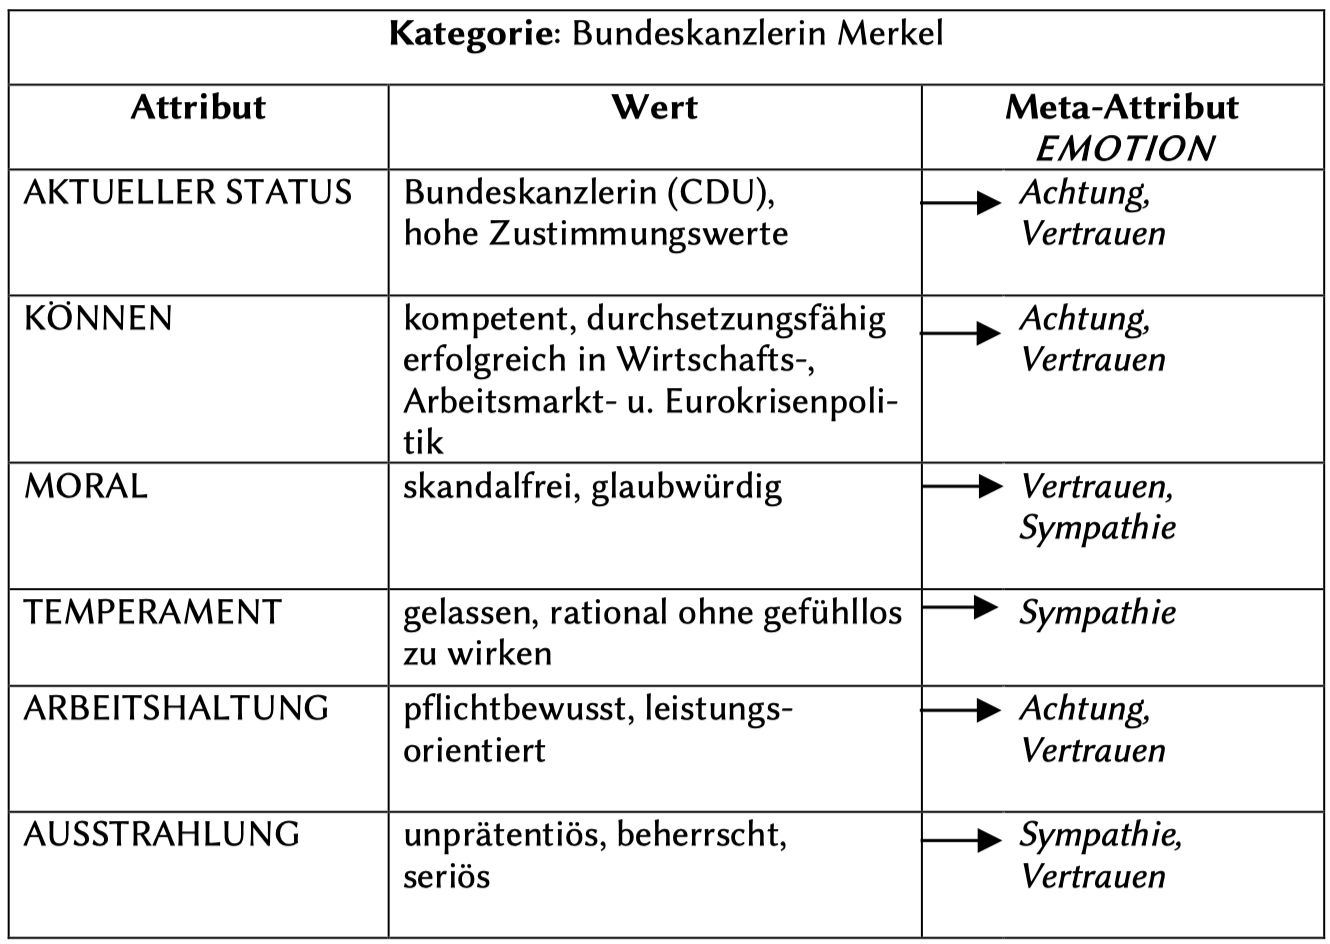
\includegraphics[width=\textwidth]{figures/media/image5.png}
  \caption{\label{fig:merkel-frame}Merkel-Ausgangs-Frame (Übersicht 5 aus \citealt[312]{kleinFrameUndFraming2018}). Legende: Pfeil: Kausalrelation (Ursache{\slash}Grund → Wirkung{\slash}Folge)}
\end{figure}

Das Ziel bestehe nun für die CDU darin,

\begin{quote}
die in den Ausgangsframes erfassten Vorstellungen im Sinne des Wahlzieles und der Hauptausrichtung der Kampagne zu modifizieren bzw. zu optimieren und als verbessertes Bild der CDU-Politik und der Kanzlerin in den Köpfen möglichst vieler Wahlberechtigter zu verankern. \autocite[314]{kleinFrameUndFraming2018}
\end{quote}

Dazu können zum einen die bestehenden Attribut-Wert-Konfigurationen gestärkt oder modifiziert werden, zum anderen können neue Attribut-Wert-Paare etabliert werden. Die beim Framing eingesetzten kommunikativen Mittel reichen dabei von einzelnen Formulierungen in Broschüren und Wahlreden bis hin zu Erzählungen aus dem Privatleben im Fernsehen sowie visuellem Framing auf Plakaten und im Fernsehen. Eine Kombination verschiedener Mittel wurde etwa eingesetzt, um \textsc{Wählernähe} als neues Attribut im Frame zu etablieren:

\begin{quote}
Merkels weithin hoch geschätzte Eigenschaft, unprätentiös zu sein, erleichterte Framing in Richtung ‚Normalisierung` der Bundeskanzlerin. Das geschah primär in Texten, aber auch in Bildern. Auf Merkels eigens für die Wahlkampagne eingerichteter sog. ‚Homepage` und in der damit text- und bild-identischen, massenhaft verteilten Merkel-Broschüre wird einerseits die entscheidungsstarke, durchsetzungsfähige Politikerin nicht verleugnet („ich will\ldots``; „ich entscheide...``), andererseits ist sie, wenn es um Privates geht, eine ‚wie du und ich`: „Ich koche sehr gern, am liebsten Rouladen und Kartoffelsuppe.`` Ihr Ehemann, ein „Konditorsohn`` beschwert sich, „auf dem Kuchen sind immer zu wenig Streusel.`` \autocite[315-316]{kleinFrameUndFraming2018}
\end{quote}

Ob es tatsächlich so simpel gelingen kann, neue bzw. modifizierte Frames in den Köpfen der Wähler*innen zu verankern, bleibt aber letztlich offen.\footnote{Klein verweist allerdings auf den Wahlerfolg der CDU als Indikator: „Zwar pflegen Wahlsiege viele Mütter und Väter zu haben, doch wäre es bei einem so klaren und hohen Wahlsieg wie dem der Union 2013 wenig rational anzunehmen, dass alles mögliche Andere für den Erfolg der Kampagne verantwortlich war, nur nicht das strategische Framing.`` \autocite*[327]{kleinFrameUndFraming2018}.}

Einen im Vergleich deutlich stärker deskriptiv ausgerichteten Framing-Begriff präsentieren Ziem et al. \autocite*{ziemMedienFramesAlsSemantische2018}. Zwar stimmen sie Klein grundsätzlich darin zu, dass „während Frames Wissensstrukturen repräsentieren und modellieren, {[}\ldots{]} sich der Begriff des Framing insbesondere auf den Prozess der Entstehung und Verfestigung dieser Strukturen {[}richtet{]}`` \autocite[159]{ziemMedienFramesAlsSemantische2018}. Sie differenzieren jedoch zwischen einem strategisch-intentionalen Framing im Sinne des „Begriffe besetzen`` \autocite{liedtkeBegriffeBesetzenStrategien1991}, wie es in den hier bisher betrachteten Framing-Konzepten angedacht ist, und einem Framing, das „emergent{[}es{]} Ergebnis des Sprachgebrauchs`` \autocite[159]{ziemMedienFramesAlsSemantische2018} und insofern ein Fall von „Begriffswandel`` \autocite{kellerSprachwandelUnsichtbarenHand2003} ist. Ähnlich wie Klein konzeptualisieren sie Framing als die variierende Instantiierung von Frame-Slots und -Fillern und nutzen für dessen analytische Erfassung und Beschreibung \emph{FrameNet}. Sie können so zeigen, dass im Kontext der Snowden-Affäre in der New York Times der \FN{Gathering\_up}-Frame mit anderen FE realisiert wird als in einem aus dem Open American National Corpus bezogenen Vergleichskorpus und etwa die Slots \textsc{Agens} und \textsc{Individuen}, d.\,h. die sammelnden Akteure und die gesammelten Objekte, deutlich häufiger realisiert werden, während FE wie \textsc{Zweck}, \textsc{Quelle} oder \textsc{Zeit} seltener instantiiert werden als im Vergleichskorpus.

Klein und Ziem verbinden die Frame- und die Framing-Theorie auf durchaus ähnliche Weise miteinander, geben jedoch keine bündige Definition für ihren Framing-Begriff. Für diese Arbeit sei daher als Arbeitsdefinition festgehalten, dass Framing die potentiell strategische Instantiierung eines Frames mit bestimmten Slots und Fillern meint. Instantiiert werden natürlich zunächst Token-Frames; durch Abstraktion kann aber auch auf Type-Frames geschlossen werden, die dann für einzelne Diskursbereiche ein bestimmtes Framing ausweisen. Hinsichtlich der Praxisorientierung des Framing-Begriffs folgt die Arbeitsdefinition Ziem et al. und fügt sich in den deskriptiven Gesamtansatz der vorliegenden Arbeit ein. Framing ist so zwar durchaus an sprachliches Handeln gebunden, kann aber zugleich (auch) als emergentes, unintentionales Phänomen verstanden werden. Diese Definition weist weitgehende Übereinstimmungen mit Busses Ausführungen zur Perspektivierbarkeit von Frames (\chapref{perspektivierung-kontext-und-frame-wandel}) auf, die er als „Aktivierung bestimmter Sub-Sets von Slots / Attributen aus der Gesamt-Menge von Slots / Attributen eines \emph{type}-Frames`` oder durch die „Füllung der Slots mit spezifischen (Sets von) Werten`` definiert \autocite[622]{busseFrameSemantikKompendium2012}. Wengelers Einwand, das Framing-Konzept eröffne der Linguistik kaum neue Analysemöglichkeiten, sondern habe nicht zuletzt „aufgrund seines modernen Touchs`` \autocite*[27]{wengelerWarnungVorFraming2022} Einzug in Frame-semantische Arbeiten erhalten, ist also nicht völlig von der Hand zu weisen. Meines Erachtens sind jedoch die Anschließbarkeit an die Kommunikations- und Medienwissenschaft inklusive der Unterlegung ihrer Framing-Theorie mit einem ausgearbeiteten Wissensmodell inklusive der präzisen Berücksichtigung sprachlicher Zeichen \autocite[176]{ziemMedienFramesAlsSemantische2018}, die gute Kommunizierbarkeit des Begriffs und letztlich auch die terminologische Eleganz („Frame ist Struktur. Framing ist Handeln.``, \citealt[289]{kleinFrameUndFraming2018}) gute Gründe, den Begriff auch in der Linguistik zu nutzen.

\section[Semantik, Pragmatik und das \emph{corpus-driven} Paradigma]{Distributionelle Semantik, Korpuspragmatik und das \emph{corpus-driven} Paradigma}\label{distributionelle-semantik-korpuspragmatik-und-das-corpus-driven-paradigma}
\subsection{Distributionelle Semantik}\label{distributionelle-semantik}

In den bisherigen Kapiteln wurde die Grundlage dafür gelegt, in Diskursen konstituierte und verhandelte Bedeutung mithilfe eines ausdifferenzierten linguistischen Modells beschreiben zu können. Auch wenn diesen Modellen zumeist die Annahme kognitiver, individueller Wissensbestände zugrundeliegt, wird zu ihrer Ermittlung in Frame-semantischen Analysen auf linguistische Methodik und Diskurskorpora zurückgegriffen (siehe \chapref{frames-und-kognition}). Da dabei auch quantitativ-korpuslinguistische Ansätze wie Keyword- oder Kollokations-Analysen auf fruchtbare Weise herangezogen werden \autocites[siehe u.\,a.][]{czuloEinflussExtremistischerGewaltereignisse2020, ziemMedienFramesAlsSemantische2018, ziem3WortschatzII2017, storjohannPrasenzUndAbsenz2013}, liegt es nicht fern, über eine vertiefte Integration Frame-semantischer Ansätze mit korpuslinguistischen Zugängen zur Semantik nachzudenken. Für letztere ist insbesondere das Paradigma der distributionellen Semantik ein wichtiger Rahmen. Seine Grundlagen wurden bereits in den 1950er Jahren gelegt, in denen die Distribution von Wörtern als höchst relevant für ihre semantische Beschreibung erkannt worden ist. Es ist dabei zum einen die Tradition des amerikanischen Strukturalismus, zum anderen die des britischen Kontextualismus, die die Entstehung distributionell-semantischer Ansätze prägen. Von amerikanisch-strukturalistischer Seite stellt Zellig Harris den Zusammenhang zwischen Bedeutung und Distribution heraus: „difference of meaning correlates with difference of distribution`` \autocite*[156]{harrisDistributionalStructure1954}. Diese Erkenntnis ist, so Lenci, der Ausgangspunkt für die ‚Distributionelle Hypothese`, die er folgendermaßen zusammenfasst: „Lexemes with similar linguistic contexts have similar meanings.`` \autocite[152]{lenciDistributionalModelsWord2018}. Etwas weiter gefasst formuliert Sahlgren:

\begin{quote}
The main point of this hypothesis is that there is a correlation between distributional similarity and meaning similarity, which allows us to utilize the former in order to estimate the latter. \autocite[33]{sahlgrenDistributionalHypothesis2008}
\end{quote}

Auch die Arbeiten John Rupert Firths, dem Begründer des britischen Kontextualismus, spielen in distributionell-semantischen Ansätzen eine wichtige Rolle. Er hat insbesondere die Bedeutung des Kotextes für die Semantik erkannt und in der berühmten Formel „You shall know a word by the company it keeps`` \autocite[11]{firthSynopsisLinguisticTheory1957} zusammengefasst. Auf Firth geht dabei auch das für die Korpuslinguistik zentrale Konzept der Kollokation zurück und er konstatiert, dass \emph{collocational meaning} eine von mehreren Bedeutungsdimensionen ist:

\begin{quote}
The following sentences show that part of the meaning of the word \emph{ass} in modern colloquial English can be by collocation:

(i) An ass like Bagson might easily do that.

(ii) He is an ass.

(iii) You silly ass!

(iv) Don't be an ass!

One of the meanings of \emph{ass} is its habitual collocation with an immediately preceding \emph{you silly}, and with other phrases of address or of personal reference. Even if you said „An ass has been frightfully mauled at the Zoo``, a possible retort would be, „What on earth was he doing?{}`` \autocite[194-195]{firthPapersLinguistics193419511957}
\end{quote}

In kontextualistischer Perspektive sind sprachliche Äußerungen dabei immer funktional zu denken und in rekurrente situative sowie diese umfassende kulturelle Kontexte eingebettet:

\begin{quote}
That is what language really means to us -- a way of doing things, a way of getting things done, a way of behaving and getting others to behave, a way of life. {[}\ldots{]} We can only arrive at some understanding of \emph{how} it works, if we establish with certainty that the facts of speech we are studying can be observed or regarded in actual patterns of behaviour. We must take our facts from speech sequences, verbally complete in themselves and operating in contexts of situation which are typical, recurrent, and repeatedly observable. Such contexts of situation should themselves be placed in categories of some sort, sociological and linguistic, within the wider context of culture. \autocite[35]{firthSynopsisLinguisticTheory1957}
\end{quote}

Diese kontextuelle Bedeutungsdimension unterscheidet er jedoch von der kotextuellen, über Kollokationen aufspürbaren\footnote{So konstatiert er: „It must be pointed out that meaning of collocation is not at all the same thing as contextual meaning, which is the functional relation of the sentence to the processes of a context of situation in the context of culture`` \autocite[195]{firthPapersLinguistics193419511957}.} und möchte letztere auch nicht mit konzeptueller Bedeutung verwechselt wissen:

\begin{quote}
Meaning by collocation is an abstraction at the syntagmatic level and is not directly concerned with the conceptual or idea approach to the meaning of words. \autocite[196]{firthPapersLinguistics193419511957}
\end{quote}

Distributionell-semantische Modelle lassen sich gemäß der von ihnen gemessenen distributionellen Achse in zwei Gruppen unterteilen: syntagmatische und paradigmatische Modelle \autocite[40]{sahlgrenDistributionalHypothesis2008}. Syntagmatische Modelle bilden dabei das gemeinsame Vorkommen von Wörtern ab, also z.\,B. dass das Wort \emph{festgenommen} mit Wörtern wie \emph{wurde}, \emph{Polizei}, \emph{Verdächtigen}, \emph{Personen} oder \emph{sieben} vorkommt (siehe \tabref{tab:collocations_neighbors}). Sie sind in Form der Kollokationsanalyse fester Bestandteil des (korpus\mbox{-})linguistischen Methodeninventars (siehe zur Methode der Kollokationsanalyse ausführlicher \chapref{kollokationen-als-syntagmatische-distributionelle-muster}). Paradigmatische Modelle hingegen fragen nicht nach den Nachbarn eines Wortes in Texten, sondern danach, welche Wörter ähnliche Nachbarn haben. Dazu werden Wörter i.d.R. in Vektoren, also Listen von Zahlen, überführt. Sie können dann in einem gemeinsamen vektorgeometrischen Raum abgebildet werden, wobei ihre Position in diesem Raum auf ihren Kotexten beruht und Wörter mit ähnlichen Kotexten nah beieinander positioniert sind. Die paradigmatische Ähnlichkeit bzw. Nähe im Vektorraum entspricht dabei diskurs- bzw. korpusspezifischer funktionaler Äquivalenz \autocite[587]{bubenhoferSemantischeAquivalenzGeburtserzahlungen2020}. Die nächsten paradigmatischen Nachbarn\footnote{Sinclair \autocite*[142]{sinclairTrustTextLanguage2004} nutzt auch für \emph{paradigmatische} Nachbarschaft in diesem Sinne den Begriff der Kollokation; üblicherweise -- und so auch in dieser Arbeit -- ist er aber der syntagmatischen Nachbarschaft vorbehalten.} zu \emph{festgenommen} sind in einem solchen Vektorraum Wörter wie \emph{inhaftiert}, \emph{beschuldigt}, \emph{getötet} oder \emph{geschnappt} (siehe \tabref{tab:collocations_neighbors}). Enorm an Popularität gewonnen haben paradigmatische distributionelle Modelle mit der Entwicklung moderner, ressourcensparsamer und auf neuronalen Netzen beruhender Algorithmen wie denen des \emph{Word2Vec}-Frameworks \autocite{mikolovEfficientEstimationWord2013}, mit denen sich solche Wortvektoren (Word Embeddings) berechnen lassen (siehe dazu ausführlich \chapref{word-embeddings-als-paradigmatische-distributionelle-muster}).

Allen distributionell-semantischen Modellen ist gemein, dass sie keine ‚unmittelbare`, referentielle Auskunft zur Bedeutung eines Wortes geben, sondern nur differentielle Informationen: Wir erfahren, wie Wörter in einem Korpus verteilt sind und inwiefern sich diese Verteilung von der anderer Wörter unterscheidet, können aber die Bedeutung von z.\,B. \emph{festgenommen} nicht unmittelbar ablesen. Sahlgren stellt heraus, dass sich daran der strukturalistische Charakter der distributionellen Semantik zeigt und ihr Bedeutungsbegriff dem Saussureschen Begriff des \emph{valeur} entspricht:
\largerpage[-2]
\begin{quote}
Similarly in la langue, signs are identified by their functional differences. Saussure used the term \emph{valeur} to describe the function of a sign. This is arguably the most important concept in structuralist theory, since it is a sign's valeur that defines its role within the language system. Valeurs are defined purely differentially, so that a sign has a valeur only by virtue of being different from the other signs. Such a differential view on the functional distinctiveness of linguistic elements highlights the importance of the system as a whole, since differences (i.e. valeurs) cannot exist in isolation from the system itself. A single isolated sign cannot enter into difference relations, since there are no other signs to differ from. In this view, the system itself becomes an interplay of functional differences \autocite[38]{sahlgrenDistributionalHypothesis2008}
\end{quote}

Dies macht Word Embeddings gerade für kulturbezogene Forschung zu einer hervorragenden Methode, denn die „fundamental insight that meaning is not immanent within words and phrases but rather coheres within a broader cultural system is inherent in any word embedding analysis'' \autocite[914]{kozlowskiGeometryCultureAnalyzing2019}. Ein weiteres Charakteristikum distributioneller Bedeutungsmodelle ist, dass sie durch und durch sprachgebrauchsbasiert, induktiv und korpusspezifisch sind. Sie grenzen sich somit von jeglichem Versuch einer introspektiven Sprachbeschreibung ab:

\begin{quote}
By grounding the representations in actual usage data, distributional approaches only represent what is \emph{really there} in the current universe of discourse. When the data changes, the distributional model changes accordingly; if we use an entirely different set of data, we will end up with an entirely different distributional model. Distributional approaches acquire meanings by \emph{virtue} of being based entirely on noisy, vague, ambiguous and possibly incomplete language data. \autocite[50]{sahlgrenDistributionalHypothesis2008}
\end{quote}

Die zentrale Stellung des Korpus in der distributionellen Semantik und die funktionale Perspektive auf Sprachzeichen korrespondiert eng mit theoretischen Überlegungen aus dem Bereich der Korpuspragmatik, die im folgenden Kapitel dargestellt werden sollen.

\subsection{Korpuspragmatik}\label{korpuspragmatik}

Den Begriff der Korpuspragmatik definieren Felder et al. \autocite*{felderKorpuspragmatikParadigmaZwischen2012} in der Einleitung zum von ihnen herausgegebenen gleichnamigen Sammelband als

\begin{quote}
linguistischen Untersuchungsansatz, der in digital aufbereiteten Korpora das Wechselverhältnis zwischen sprachlichen Mitteln einerseits und Kontextfaktoren andererseits erforscht und dabei eine Typik von Form-Funktions-Korrelationen herauszuarbeiten beabsichtigt. Solche Kontextfaktoren betreffen potenziell die Dimensionen \emph{Handlung}, \emph{Gesellschaft} und \emph{Kognition}. Die Analyse bedient sich insbesondere einer Kombination qualitativer und quantitativer Verfahren. \autocite[4-5]{felderKorpuspragmatikParadigmaZwischen2012}
\end{quote}

Ausgegrenzt aus dem Zielgebiet korpuspragmatischer Studien werden somit solche korpuslinguistischen Ansätze, die ein „sprachstrukturimmanentes Interesse haben``, also etwa zu lexikologischen oder grammatischen Fragestellungen arbeiten \autocite[4]{felderKorpuspragmatikParadigmaZwischen2012}. Sprachliche Bezugsgröße ist für sie der Diskurs im Sinne des Sprachgebrauchs \autocite{fasoldSociolinguisticsLanguage1990}, den sie mit van Dijk \autocite*{vandijkDiscourseContextSociocognitive2008} als multimodal begreifen und dessen „Handlungscharakter`` sie hervorheben \autocite[5]{felderKorpuspragmatikParadigmaZwischen2012}. Eine weitere Grundannahme der Korpuspragmatik ist im Anschluss an Feilke \autocite*{feilkeSpracheAlsSoziale1996} und Tomasello \autocite*{tomaselloKonstruktionsgrammatikUndFrueher2006} „das Theorem {[}\ldots{]}, dass die Regelhaftigkeit von Sprache sich aus der Regelhaftigkeit von Verwendungssituationen ableitet`` \autocite[5]{felderKorpuspragmatikParadigmaZwischen2012}. Hierauf stützen sie auch die zentrale Rolle von Kontexten als „verstehensrelevante Deutungsrahmen`` \autocite[6]{felderKorpuspragmatikParadigmaZwischen2012} und heben die epistemische Rolle sprachlicher Zeichen und Muster hervor:

\begin{quote}
Bedenkt man in diesem Zusammenhang, dass ein großer Teil unseres individuellen Wissens auf der Rezeption von Sprachzeichen, wie sie in sprachlichen Äußerungen mündlicher und schriftlicher Art verbreitet werden, basiert, so ist evident, dass die auf diese Weise gewonnenen Wissensbestände und Erfahrungen in kommunikativen Formulierungsroutinen reproduziert und dadurch teilweise zu „kollektiven`` Wissensbeständen bzw. Erfahrungsmustern verdichtet werden. \autocite[6]{felderKorpuspragmatikParadigmaZwischen2012}
\end{quote}

Dieser epistemologische Fokus sowie die Handlungs- und Gesellschaftsorientierung der Korpuspragmatik machen auch die Forschungsgegenstände einer Diskurslinguistik nach Foucault \autocite{warnkeDiskurslinguistikNachFoucault2007a} zum Thema der Korpuspragmatik. Zu den wissensorientierten diskurslinguistischen Arbeiten konstatieren sie jedoch:

\begin{quote}
In diesem Bereich ist das korpuslinguistische Vorgehen nicht sonderlich weit verbreitet. Das erklärt sich leicht dadurch, dass Wissensbestände nur interpretativ aus Texten plausibel gemacht werden können, ein qualitativer Zugang also unumgänglich erscheint. Allerdings haben sich hier korpuslinguistische Methoden zur Vorstrukturierung und Identifizierung zentraler Diskursmuster bewährt, in denen Wissenskonfigurationen ausgedrückt sind. \autocite[14]{felderKorpuspragmatikParadigmaZwischen2012}
\end{quote}

Meines Erachtens wirft diese Konzeption zur Rolle korpuslinguistischer Verfahren jedoch mehrere Fragen auf. Erstens sind korpuslinguistische Verfahren m.\,E. nicht mit einem quantitativen Zugang gleichzusetzen. So wird -- gerade in den englischsprachigen \emph{corpus-assisted discourse studies} (CADS) -- die Bedeutung der Lektüre von Konkordanzen oder auch längerer Textpassagen immer wieder hervorgehoben \autocite[siehe etwa][7]{gillingsTakingRoadLess2024}. Zweitens wird hier m.\,E. eine -- im Bereich der diskurslinguistischen Wissensanalyse allerdings in der Tat weit verbreitete -- Fehlannahme reproduziert, die das Verhältnis von quantitativer Korpuslinguistik, Interpretation und Wissensbeständen als Analyseobjekt betrifft. So ist es zwar in der Tat so, dass „Wissensbestände nur interpretativ aus Texten plausibel gemacht werden können`` -- dies bedeutet aber nicht, dass dies auf der Basis eingehender, qualitativer Textlektüren erfolgen muss. Auch quantitative, aus Texten gewonnene Daten müssen interpretiert werden und auch aus ihnen können Wissensbestände erschlossen werden (siehe dazu auch \chapref{begriffsklaerungen-quantitativ-und-qualitativ-corpus-driven-und-corpus-based-sowie-die-rolle-von-hermeneutik}). Letztlich ist auch zu fragen, warum quantitative Verfahren, wenn sie doch eine „Vorstrukturierung und Identifizierung zentraler Diskursmuster {[}\ldots{]}, in denen Wissenskonfigurationen ausgedrückt sind``, leisten können, nicht geradezu dafür prädestiniert sein sollten, um in epistemologisch-diskurslinguistischen Analysen eingesetzt zu werden. So ist doch zu bezweifeln, dass qualitative Methoden mehr leisten können, als Texte zu strukturieren, um in ihnen relevante Diskursmuster zu identifizieren. Einen irgendwie gearteten ‚direkten` Zugang zum diskursiv verhandelten Wissen bieten auch sie nicht.

Während bei Felder et al. \autocite*[4-5]{felderKorpuspragmatikParadigmaZwischen2012} die bevorzugte „Kombination qualitativer und quantitativer Verfahren`` gar definitorischen Rang für das korpuspragmatische Paradigma erhält, hat sich in den Arbeiten von Noah Bubenhofer und Joachim Scharloth ein deutlich stärker quantitativ akzentuierter Begriff der Korpuspragmatik herausgebildet. Sie definieren einen korpuspragmatischen Zugang wie folgt:

\begin{quote}
Die Korpuspragmatik deutet signifikant häufig auftretende sprachliche Muster in Korpora als Ergebnis rekurrenter Sprachhandlungen der Autorinnen und Autoren der im Korpus enthaltenen Texte bzw. der sie autorisierenden Institutionen und Gruppen. Sie geht davon aus, dass sich pragmatische Informationen „im pragmatischen Mehrwert oder Gebrauchswert von Einheiten aller sprachlicher Strukturbereiche`` (Feilke 2000: 78) zeichenhaft manifestiert. Damit werden pragmatische Spuren an der sprachlichen Oberfläche als Muster, in die sich ein Gebrauchswert eingeschrieben hat, sichtbar (vgl. zu dieser Rehabilitierung der Textoberfläche auch den Sammelband von Feilke{\slash}Linke 2009). Diese „Sprachgebrauchsmuster`` (Bubenhofer 2009) werden damit als Ergebnis von sprachlich-sozialem Handeln gelesen und gedeutet. \autocite[148-149]{bubenhoferKorpuslinguistischeDiskursanalyseNutzen2013}
\end{quote}

Auch Bubenhofer \& Scharloth heben also mit Feilke den Nexus zwischen wiederholtem (sprachlichen) Handeln und sprachlichen Mustern auf der Textoberfläche hervor. Mit dem statistischen Konzept der signifikanten Häufigkeit ist bei ihnen allerdings ein quantitativer, d.\,h. auf Frequenzen operierender, Zugang vorausgesetzt. Dieser erlaubt zugleich ein induktives, \emph{corpus-driven} \autocite{tognini-bonelliCorpusLinguisticsWork2001} Vorgehen, für das die Autoren sich aussprechen, da es Befunde ermöglicht, „die entweder quer zu den vorher existierenden Erwartungen stehen und die Grundlage für neue Hypothesen sind, oder im besten Fall sogar solche Evidenzen, die die Bildung neuer interpretativer linguistischer Analysekategorien nahelegen`` \autocite[149]{bubenhoferKorpuslinguistischeDiskursanalyseNutzen2013}. Diese Potenziale sind für Frame-semantische Diskursanalysen äußerst vielversprechend, da sie helfen können, FE eines Frames aufzudecken. So warnen auch Scholz \& Ziem in Hinblick auf rein deduktive Analysen, es könne

\begin{quote}
sich ein gravierendes methodologisches Problem ergeben, wenn die Annotationen ausschließlich auf den vorgegebenen Kategorien -- d.\,h. den Prädiktoren in Matrixframes und Frame-Elementen in FrameNet-Frames -- beruhen: Das vordefinierte Set an Leerstellen bzw. Frame-Elementen determiniert den Such- und Annotationsbereich derart, dass außerhalb dessen keine Annotationen vorgenommen werden können. Zugespitzt formuliert: Es lässt sich nur das finden, was mittels der vorgegebenen Annotationskategorien auch gesucht wird. Dieses Dilemma lässt sich nur mittels einer induktiven Untersuchungsheuristik vollständig beheben. \autocite[306]{scholzVokabularImDiskurshistorischen2015}
\end{quote}

Ein weiterer gewichtiger Vorteil liegt m.\,E. darin, dass den Ergebnissen von \emph{corpus-driven} Methoden „sämtliche Zeichenkonfigurationen {[}\ldots{]}, die sich bei der Anwendung vorher festgelegter Algorithmen ergeben`` \autocite[149]{bubenhoferKorpuslinguistischeDiskursanalyseNutzen2013}, zugrundeliegen. Wenn sie also zur Bildung linguistischer Kategorien im Sinne von FE geeignet sind und auf sprachlichen Zeichenkonfigurationen beruhen, könnten sie auch helfen, sich dem Ziel einer linguistischen Epistemologie, alle sprachlichen Mittel zu identifizieren, die mit einem Frame bzw. den einzelnen FE verbunden sind, zumindest deutlich näher zu kommen, als es in qualitativen Ansätzen je geleistert werden könnte. Die folgenden beiden Kapitel werden Bubenhofers \autocite*{bubenhoferSprachgebrauchsmusterKorpuslinguistikAls2009} Begriff des Sprachgebrauchmusters, der in dieser Variante der Korpuspragmatik zentral ist, sowie den von den Autoren verfolgten \emph{corpus-driven} Ansatz darstellen.

\subsection{Sprachgebrauchsmuster}\label{sprachgebrauchsmuster}

In der germanistischen korpusbasiert arbeitenden Diskurslinguistik ist das bereits angesprochene \emph{corpus-driven} Paradigma, das im folgenden Kapitel noch ausführlicher vorgestellt werden wird, insbesondere mit den Arbeiten Noah Bubenhofers und Joachim Scharloths verbunden \autocites[siehe zu \emph{corpus-driven} Zugängen in der Phraseologie und Grammatik etwa][]{belicaKorpusanalytischeZugangeSprachlichem2008, brunnerCorpusDrivenStudyMultiWord2007, kupietzGebrauchsbasierteGrammatikStatistische2009}. Die grundlegende Operationalisierung korpuslinguistischer Zugänge für die Diskursanalyse leistet dabei Bubenhofer \autocite*{bubenhoferSprachgebrauchsmusterKorpuslinguistikAls2009}, der in einer \emph{corpus-driven} verfahrenden Analyse Diskurse anhand von Sprachgebrauchsmustern, d.\,h. musterhaftem Sprachgebrauch auf der sprachlichen Oberfläche, rekonstruiert. Eine Besonderheit stellt auch der Verzicht auf bzw. sogar die explizite Ablehnung einer thematischen Definition von Diskursen und Diskurskorpora, wie sie im einschlägigen Aufsatz von Busse und Teubert \autocite*{busseIstDiskursSprachwissenschaftliches1994} für die germanistische Diskurslinguistik gefordert und geprägt wird, dar. Als Gründe führt Bubenhofer die Unvoreingenommenheit einer solchen Analyse an, die die Replizierung bereits angenommener Diskurse und Diskursstrukturen vermeidet:

\begin{quote}
Die Frage nach der Repräsentativität des Korpus zeigt, dass Busse/ Teubert (1994, 14f.) diese nach inhaltlichen Kriterien festlegen, was zu einer manuellen Auswahl von „relevanten`` Texten führt. Diese Beschränkung ist nicht nur unnötig, sondern auch kritisch, wenn das Ziel einer Diskursanalyse darin besteht, auch verborgene und unauffällige Strukturen aufzuzeigen. Relevanzempfinden ist ein Ergebnis diskursiver Formationen. Dieses als Kriterium zu wählen, bedeutet, die offensichtlichen Strukturen des Diskurses zu replizieren. \autocite[36]{bubenhoferSprachgebrauchsmusterKorpuslinguistikAls2009}
\end{quote}

Sprachgebrauchsmuster definiert Bubenhofer als „textoberflächlich{[}e{]} Indikator{[}en{]} für soziales Handeln`` \autocite*[55]{bubenhoferSprachgebrauchsmusterKorpuslinguistikAls2009}, und beschreibt ihre diskursive Funktion mit Linke als „minimale Kristallisationskerne`` \autocite*[40]{linkeBegriffsgeschichteDiskursgeschichteSprachgebrauchsgeschichte2003} von Diskursen. In der \emph{Parole} zu findende Sprachgebrauchsmuster ermöglichen somit einen „Zugriff auf epistemisches Wissen {[}\ldots{]} und damit auf Diskurse`` \autocite[53]{bubenhoferSprachgebrauchsmusterKorpuslinguistikAls2009}:

\begin{quote}
Sprachgebrauchsmuster sind Ausdruck sozialen Handelns und bestimmte Sprachgebrauchsmuster können deshalb als Indikatoren für bestimmtes soziales Handeln gelesen werden. \autocite[53]{bubenhoferSprachgebrauchsmusterKorpuslinguistikAls2009}
\end{quote}

Mit dem Ziel, idiomatische Prägungen im Sinne von Feilke \autocite*{feilkeSprachlicherCommonSense1993} abzubilden, betrachtet Bubenhofer ausschließlich Mehrworteinheiten als Sprachgebrauchsmuster. Operationalisiert werden diese für den korpuslinguistischen Zugriff als signifikante N-Gramme, also in einzelnen Teilkorpora überzufällig häufig unmittelbar aufeinander folgende Token. Die signifikanten Mehrworteinheiten als solche stellen allerdings noch keine Sprachgebrauchsmuster dar, sondern erhalten diesen Status erst nach ergänzenden kategorisierenden und interpretierenden \emph{corpus-based} Analysen.

Ausgehend von den Sprachgebrauchsmustern gelingt es Bubenhofer so, ein thematisch heterogenes Zeitungskorpus in unterschiedliche Teile -- in seinem Verständnis ‚Diskurse` -- zu gliedern und zu beschreiben. Für den Zeitraum 2003--2005 und das Auslandsressort der NZZ (\textsc{Neue Zürcher Zeitung}) fördert seine Analyse z.\,B. die Mehrworteinheiten \emph{Kampf gegen Terrorismus}, \emph{im Irak die}, \emph{Präsident Bush in} und \emph{Usama bin Ladin} zu Tage, die in diesem Teilkorpus signifikant häufiger als im restlichen Korpus auftreten und sich unschwer auf den Irakkrieg zurückführen lassen \autocite[209-210]{bubenhoferSprachgebrauchsmusterKorpuslinguistikAls2009}. Solche Gruppen von Sprachgebrauchsmustern können sodann als „Hinweise auf Diskurse`` \autocite[295]{bubenhoferSprachgebrauchsmusterKorpuslinguistikAls2009} aufgefasst werden, etwa zu Themen wie ‚Krieg und Gewalt` oder ‚Sorgen und Probleme` und sie übernehmen in diesen Diskursen je spezifische, mitunter auf subtile Art ausdifferenzierte Funktionen:

\begin{quote}
Bei der Analyse der Kontextualisierungsprofile von \emph{Kampf gegen X}, \emph{Kampf dem X} und \emph{Kampf mit X} haben sich deutliche Differenzen im Gebrauch gezeigt. Dabei handelt es sich nicht nur um semantische Präferenzen {[}\ldots{]}, sondern um pragmatisch unterschiedliche Funktionen. So wird der \emph{Kampf gegen den Terror} im Ausdruck \emph{Kampf dem Terror} zur Parole; der Ausdruck findet sich besonders häufig in argumentativen Kontexten und zeigt eine Distanzierung oder Kritik an. \autocite[303]{bubenhoferSprachgebrauchsmusterKorpuslinguistikAls2009}
\end{quote}

Dass Bubenhofers Diskursbegriff dabei letztlich auf einer formalen Ebene bleibt und sich gegen thematische Diskursdefinitionen dezidiert abgrenzt, führt dazu, dass die beschriebenen Diskurse mitunter eher vage umrissen sind und einander überlappen. So resümiert er:

\begin{quote}
Der induktive Zugang ist also nicht vorurteilslos, aber er definiert seine Grundannahmen anders als es z.\,B. semantisch-tiefenstrukturelle Analysen tun. Und dieser Zugang führt dann auch zu einem bunten Strauß an Sprachgebrauchsmustern, die einerseits eher Kristallisationspunkte des inhaltlich Sagbaren, andererseits der Sprechweisen, der diskursiven Praxis darstellen. Diese Heterogenität ist auf der Ebene der Analyse nicht immer einfach zu handhaben und es ist kaum möglich, daraus homogene Diskursbeschreibungen abzuleiten. \autocite[311]{bubenhoferSprachgebrauchsmusterKorpuslinguistikAls2009}
\end{quote}

Eine solche Einschränkung wäre für die Diskurslinguistik, die ja i.d.R. an der Untersuchung aktueller und gesellschaftlich relevanter thematischer Diskurse interessiert ist, durchaus hinderlich. Es ist m.\,E. jedoch zu prüfen, ob die von Bubenhofer vorgenommene Trennung zwischen thematischen und entlang von Sprachgebrauchsmustern definierten Diskursen wirklich notwendig ist. So sind Themen ja ebenfalls Bedeutungskomplexe -- und wenn Sprachgebrauchsmuster „kleinste semantische Einheiten`` \autocite[336]{bubenhoferSprachgebrauchsmusterKorpuslinguistikAls2009} sind, sollte es möglich sein, anhand von Sprachgebrauchsmustern auch klassische Themen zu rekonstruieren. Es erscheint aus umgekehrter Blickrichtung ja auch unplausibel, dass sich Themen nicht in musterhaftem Sprachgebrauch, allen voran dem rekurrenten Gebrauch eben thematisch einschlägiger Lexik, niederschlagen sollten. In der vorliegenden Arbeit gilt es also zu prüfen, ob in der sprachlichen Oberfläche und der Distribution von Wörtern sowie unter Einbezug neuerer methodischer Entwicklungen nicht doch ausreichend semantische Informationen vorliegen, um aus ihnen auch klassische Themen bzw. thematische Frames wie einen Extremismus-Frame rekonstruieren zu können. Der \emph{corpus-driven} Ansatz, der dabei zugrundegelegt wird, soll im folgenden Kapitel näher erläutert werden, wobei auch auf grundlegende Annahmen des britischen Kontextualismus sowie seiner korpuslinguistischen Weiterentwicklung durch Sinclair und Tognini-Bonelli eingegangen wird.

\subsection{\texorpdfstring{Der \emph{corpus-driven} Ansatz}{Der corpus-driven Ansatz}}\label{der-corpus-driven-ansatz}

Methodologischer Rahmen einer korpuslinguistischen und -- Bubenhofer und Scharloth folgend -- auch einer korpuspragmatischen Perspektive auf Sprache ist der \emph{corpus-driven}-Ansatz, wie er von Tognini-Bonelli \autocite*{tognini-bonelliCorpusLinguisticsWork2001} in Abgrenzung zum \emph{corpus-based} Ansatz vorgeschlagen wurde. Beide Vorgehensweisen werden im Folgenden vorgestellt, bevor sie in \chapref{begriffsklaerungen-quantitativ-und-qualitativ-corpus-driven-und-corpus-based-sowie-die-rolle-von-hermeneutik} auch von der Differenzierung qualitativ -- quantitativ unterschieden werden.

Das \emph{corpus-based}-Paradigma wird von Tognini-Bonelli als eine Methodologie gefasst, die Korpora hauptsächlich dafür verwendet, bereits existente Hypothesen zu elaborieren, zu prüfen oder zu belegen. Diese Herangehensweise

\begin{quote}
avails itself of the corpus mainly to expound, test or exemplify theories and descriptions that were formulated before large corpora became available to inform language study. \autocite[65]{tognini-bonelliCorpusLinguisticsWork2001}
\end{quote}

Das Korpus dient hier im Wesentlichen dazu, den Anteil, den Intuition und Sprachgefühl in introspektiv verfahrenden Analysen haben, durch einen empirischen Zugang zu ersetzen bzw. ergänzen. Theorien müssen nun operationalisiert und in einem entsprechend aufbereiteten Korpus untersucht werden:

\begin{quote}
Traditionally, linguistic theories are the result of reflection by a scholar after absorbing a great deal of experience of language and languages, and testing the implications and consequences with reference to the intuition of competent or native speakers. The precise nature of the language experience is impossible to ascertain because it figures only as part of the linguist's credentials, and not as part of the methodology of research. If a corpus was to be used to evaluate one of this class of theories, the theory would have to be put into an explicit form so that those aspects of corpus patterning that it covered could be distinguished from those where the theory did not cover, or was at variance with, the evidence. Such a relationship between theory and data is the classical one in linguistics. \autocite[65]{tognini-bonelliCorpusLinguisticsWork2001}
\end{quote}

Korpuslinguistik hat in diesem Ansatz also den klaren Status einer Methode, deren Verdienst es ist, linguistisches Arbeiten empirisch zu fundieren, was zur Widerlegung oder Präzisierung zahlreicher zuvor introspektiv gewonnener Annahmen über Sprache führt. Die Operationalisierung besteht dabei in der Regel in der Erstellung von Kategorien, die es in den Daten wiederzufinden gilt, sodass mithilfe empirischer Belege die Theorie bestätigt, widerlegt oder modifiziert werden kann, ohne dabei jedoch grundlegend neue theoretische Impulse zulassen zu können:

\begin{quote}
The corpus is considered useful because, on occasions, it indicates where minor corrections and adjustments can be made to the model adopted and, of course, it can also be valuable as a source of quantitative evidence. In this case, however, corpus evidence is brought in as an extra bonus rather than as a determining factor with respect to the analysis, which is still carried out according to pre-existing categories; although it is used to refine such categories, it is never really in a position to challenge them as there is no claim made that they arise directly from the data. \autocite[66]{tognini-bonelliCorpusLinguisticsWork2001}\footnote{Anzumerken ist hier, dass \emph{corpus-based}-Ansätze, wie sie heute i.d.R. praktiziert werden, durchaus geeignet sind, neue Kategorien zu entdecken. Funde in den Daten, die quer zu den bestehenden Analyseschemata liegen, stellen dann in einem iterativen Prozess einen Ausgangspunkt für die Bildung neuer Kategorien dar.}
\end{quote}

Das \emph{corpus-driven}-Paradigma setzt sich in grundlegender Weise von dieser deduktiven Herangehensweise ab. Das Korpus dient hier nicht als bloßer Datensatz, in dem Belege gefunden und Hypothesen überprüft werden können, sondern ist Grundlage für die aufzudeckenden Kategorien:

\begin{quote}
The corpus-driven approach {[}\ldots{]} aims to derive linguistic categories systematically from the recurrent patterns and the frequency distributions that emerge from language in context. \autocite[87]{tognini-bonelliCorpusLinguisticsWork2001}.
\end{quote}

Jegliche Erkenntnis wird hier also in einem engen Zusammenspiel mit den Korpusdaten bzw. aus ihnen heraus entwickelt -- „the theoretical statement can only be formulated in the presence of corpus evidence and is fully accountable to it`` \autocite[11]{tognini-bonelliCorpusLinguisticsWork2001}. Ausgangspunkt, Untersuchungsobjekt und -- in neu strukturierter, durchmusterter und informativ angereicherter Form -- letztlich auch Output einer \emph{corpus-driven} Analyse ist also die \emph{Parole}. Diese durch und durch empirische, sprachgebrauchsorientierte Ausrichtung teilt die Korpuslinguistik mit der linguistischen Diskursanalyse im Allgemeinen \autocite[27-29]{spitzmullerDiskurslinguistikEinfuhrungTheorien2011}.

Die Bedeutung der Umkehr der Erkenntnisrichtung von ‚von der Theorie zu den Daten` zu ‚von den Daten zur Theorie` geht jedoch darüber hinaus, dass neue, frequenzbasierte Methoden zur Analyse auch großer Korpora genutzt werden können. Sie eröffnen außerdem eine grundlegend neue Perspektive auf Sprache, in der sprachliche Ausdrücke immer als kontextuell geprägt gelesen werden. Trennungen wie die von Semantik und Pragmatik, von Ausdrucks- und Äußerungsbedeutung, von Ko- und Kontext werden damit zu höchstens graduellen und orientierenden Vereinfachungen; sprachliche Muster -- besonders deutlich ist dies an einzelnen Wörtern sichtbar -- sind nicht isoliert beschreibbar, sondern immer nur als Teil von Texten, situativen Kontexten und mithin Kultur:

\begin{quote}
The corpus-driven approach {[}\ldots{]} aims to derive linguistic categories systematically from the recurrent patterns and the frequency distributions that emerge from language in context. Taking this one step further, we could say that it goes along with a holistic approach to language in that the cumulative effect of repeated instances is taken to reflect the semiotic system; the text is seen as an integral part of its verbal context and, ultimately, no discontinuity is assumed between this and the wider context of situation, and the even wider context of culture. \autocite[87]{tognini-bonelliCorpusLinguisticsWork2001}\footnote{Sie scheint an dieser Stelle über Firth hinauszugehen, der \emph{collocational} und \emph{contextual meaning} noch dezidiert voneinander abgegrenzt hat (siehe \chapref{distributionelle-semantik}).}
\end{quote}

Die Bedeutung des sprachlich Musterhaften in Form dieser „repeated instances`` ist in diesem Ansatz, auf den auch Felder et al. \autocite*[3-4]{felderKorpuspragmatikParadigmaZwischen2012} bei ihrem Entwurf der Korpuspragmatik Bezug nehmen, zentral gestellt. Begründet wird dies von Tognini-Bonelli mit Verweis auf den britischen Kontextualismus, wo schon Firth ebendiese als „central evidence of what people do, how language functions and what language is about`` \autocite[89]{tognini-bonelliCorpusLinguisticsWork2001} erkannt hat. Doch was sind diese „repeated instances`` bzw. „repeated events``, die es aus dem „mush of general goings-on'' \autocite[187]{firthPapersLinguistics193419511957} herauszuarbeiten gilt? Dies fasst Tognini-Bonelli zunächst vergleichsweise simpel als ein „pattern of occurrence`` \autocite*[89]{tognini-bonelliCorpusLinguisticsWork2001}, das mindestens zwei Mal vorkommt. Um der bloßen Erfassung von „personal idiosyncrasy`` vorzubeugen, sollen die beiden Vorkommen im Korpus außerdem unabhängig voneinander, das heißt z.\,B. nicht im gleichen Text, vorkommen. Während die Möglichkeit der Erkennung von Mustern generell von der formalen Aufbereitung des Korpus abhängt, wobei einzelne Wörter oder Phrasen immer potentiell signifikant sind \autocite[89]{tognini-bonelliCorpusLinguisticsWork2001}, macht sie als die zwei zentralen Elemente musterhaften Sprachgebrauchs im Korpus die Firthschen Konzepte \emph{collocation} und \emph{colligation} aus. Kollokationen fasst sie dabei mit Clear \autocite*[277]{clearFirthPrinciplesComputational1993} als „recurrent co-occurrence of words'', die unmittelbar beobachtbar sind und vergleichsweise einfach mithilfe korpuslinguistischer Tools berechnet werden können. Den Begriff \emph{colligation} übernimmt sie direkt von Firth \autocite*[23]{firthSelectedPapersFirth1968}; er bezeichnet damit „the interrelations of syntactical categories`` in Form von Wort- und Satzarten. Für das \emph{corpus-driven}-Paradigma modifiziert Tognini-Bonelli diese Definition und rückt das Token als Einheit der \emph{Parole} zu Ungunsten abstrahierender \emph{Langue}-Kategorien in den Mittelpunkt:

\begin{quote}
In the light of corpus evidence, however, the concept of colligation is being extended to include the syntactic constraints, or indeed preferences, that a specific word, seen as a unique lexical item rather than as a member of its class, entertains within its environment. \autocite[89]{tognini-bonelliCorpusLinguisticsWork2001}
\end{quote}

Letztlich ist es die Zusammenführung von \emph{collocation} und \emph{colligation}, die für sie Muster ausmachen:

\begin{quote}
Collocational and colligational patterns will, together, form the basis of the formalisation of repeated events. Only a descriptive statement that identifies their interconnections will yield insights into meaning. The notion of `pattern' as the meeting point between lexis and grammar thus becomes central to corpus-driven linguistics. \autocite[90]{tognini-bonelliCorpusLinguisticsWork2001}
\end{quote}

Sie führt außerdem Hunston \& Francis an, die in ihrer \emph{Pattern Grammar} die „patterns of a word`` folgendermaßen definieren:

\begin{quote}
The patterns of a word can be defined as all the words and structures which are regularly associated with the word and which contribute to its meaning. A pattern can be identified if a combination of words occurs relatively frequently, if it is dependent on a particular word choice, and if there is a clear meaning associated with it. \autocite[37]{hunstonPatternGrammarCorpusDriven2000}
\end{quote}

Dadurch, dass systemlinguistische Vorannahmen hier zunächst zurückgestellt werden und stattdessen von Grunde auf nach den Kombinationsmöglichkeiten von Wörtern und ‚Strukturen` und den mit ihnen einhergehenden Bedeutungsveränderungen gefragt wird, ändert sich die „unit of currency for linguistic description`` \autocite[91]{tognini-bonelliCorpusLinguisticsWork2001}. Statt einzelne Lemmata bzw. Lexeme als Grundeinheit zu nehmen, zeigt Tognini-Bonelli an verschiedenen Beispielen, dass weder die oftmals angenommene semantische Einheit von Wortform und Lexem noch die konventionelle Trennung von Wörtern entlang von Leerzeichen durchweg haltbar bzw. semantisch sinnvoll ist. Semantische Differenzen im Flexionsparadigma eines Lexems führt sie u.\,a. am Beispiel der Wortformen \emph{facing} und \emph{faced} vor, die in unterschiedlichen Korpora jeweils unterschiedliche Gebrauchspräferenzen aufweisen:

\begin{quote}
So with \emph{facing} in the Birmingham corpus we find words such as \emph{forwards}, \emph{palms}, \emph{stood} {[}\ldots{]} which are very obviously related to position. We find also words that relate to the more abstract notion which has to do with confronting problematic areas: \emph{problems}, \emph{problem}, \emph{fear}, \emph{serious}, but as we can see they are relatively rare compared to the first group, so we could conclude that in a corpus of general English the physical meaning of \emph{facing}, indicating position and direction, is much more common than the abstract one. It is interesting to note that the same generalisation does not apply to the \emph{Economist \& WSJ} corpus where the collocates of \emph{facing} are consistently abstract. Considering now the form \emph{faced}, we do not find a parallel with the preference for the physical use either in the Birmingham or in the \emph{Economist \& WSJ} corpora {[}\ldots{]}. The two inflected forms have taken on different roles and this specialisation according to word form has also followed register boundaries between a more general purpose corpus and a more specialised corpus such as the \emph{Economist} and \emph{WSJ} corpus. \autocite[95]{tognini-bonelliCorpusLinguisticsWork2001}
\end{quote}

Dieser Befund weist zum einen auf den Wert von \emph{corpus-driven} Analysen hin, um solcher Unterschiede überhaupt gewahr zu werden. Insbesondere mit ihrer Hilfe ist es möglich, das aufzuspüren, was Feilke \& Linke (aus nicht primär korpuslinguistischer Perspektive) den „kommunikativen Mehrwert sprachlicher Performanz`` nennen. Dieser entzieht sich durch das „Faktum, dass häufig mögliche Ausdrucksvarianten im Sprachgebrauch eingeschränkt werden bzw. eine spezifische Variante präferiert wird, ohne dass eine semantische oder pragmatische Begründung auf der Hand läge`` \autocite[5-6]{feilkeOberflaecheUndPerformanz2009}, oftmals der Intuition. Der Befund ist zum anderen auch für die Frame-semantische Modellierung äußerst bedeutsam und deutet Probleme an, die eine lemmabasierte und nicht nach Register bzw. Kontext spezifizierte Zuordnung von LE zu Frames birgt (siehe auch \chapref{warum-frames}).

Der zweite erwähnte Punkt betrifft Bedeutungseinheiten, die sich über die klassischen Wortgrenzen hinaus erstrecken und für die Sinclair \autocite*{sinclairUnitsMeaning1996} den Begriff der \emph{extended units of meaning} geprägt hat. Grundlage für diese Annahme ist die Beobachtung, dass Wörter gemeinsam auftreten und dabei keine eigenständigen Bedeutungen bewahren. So definiert Tognini-Bonelli den hier einschlägigen Begriff der \emph{co-selection}, der auf Arbeiten Sinclairs zurückgeht als

\begin{quote}
the habitual selection of two or more items together. The tendency of the words to co-occur is so strong that they cannot retain independent meanings. The most obvious types of co-selection, and the ones that are traditionally acknowledged, are idioms and compounds, where two or more words with independent meaning combine to form a new meaning (e.g. \emph{vacuum cleaner}; \emph{it's raining cats and dogs}). \autocite[101]{tognini-bonelliCorpusLinguisticsWork2001}
\end{quote}

\emph{Co-selection} ist also ein graduelles Phänomen, das sich in seiner eindrücklichsten Form in idiomatischen Phraseologismen sowie den im Englischen oft nicht zusammengeschriebenen Komposita zeigt. Dass das Auftreten von Wörtern nicht voneinander unabhängig ist, lässt sich mit Leichtigkeit sprachstatistisch durch einfaches Auszählen und Signifikanztests zeigen (siehe \chapref{wie-funktioniert-die-berechnung-von-kollokationen}). Dass dieses Phänomen weiterhin höchst relevant für Fragen der Bedeutung ist, ist in einem korpuslinguistischen Zugang ebenfalls evident:

\begin{quote}
If a word has several meanings, it is easy to show that at least some of the cotext is a component of the meaning. Make a concordance of perhaps a hundred instances of the word, in a span of four words on either side. In almost all cases it will be clear from no other evidence than the cotext which meaning of the item is present, and therefore which meaning the original word partly realises. \autocites[20]{sinclairMeaningFrameworkCorpus2005}{sinclairSECTION1MULTILINGUAL1996}
\end{quote}

Die Semantik von Wörtern ergibt sich also nur im Zusammenspiel mit ihren Kotexten.\footnote{Ähnlich, wenn auch nicht auf einzelne Wortbedeutungen, sondern Frame-Evokation bezogen, weist ja auch Busse darauf hin, dass sich Semantik aus dem syntagmatischen Zusammenwirken von Wörtern ergibt (siehe \chapref{sprachoberflaechliche-bezugspunkte}).} Dieses Zusammenspiel wurde in der Linguistik bereits in zwei Richtungen gelesen. Eine eingängige Vorstellung, die auch zu Frame-semantischen Annahmen passt und in Thesauri realisiert wird, wäre, dass wer mit einem Wort auf ein Konzept referieren möchte, dabei zwangsläufig auch -- durch dieses Wort und das Konzept bestimmte -- andere Wörter nutzt. Schon in den Anfängen der distributionellen Semantik wurde in die andere Richtung gedacht und von der Betrachtung des Kotextes auf die Bedeutung des Wortes geschlossen. Dies führt Sinclair zu dem Schluss, dass die Trennung zwischen Form und Bedeutung letztlich nicht haltbar ist:

\begin{quote}
Soon it was realised that form could actually be a determiner of meaning, and a causal connection was postulated, inviting arguments from form to meaning. Then a conceptual adjustment was made, with the realization that the choice of a meaning, anywhere in a text, must have a profound effect on the surrounding choices. It would be futile to imagine otherwise. There is ultimately no distinction between form and meaning. \autocite[7]{sinclairCorpusConcordanceCollocation1991}
\end{quote}

Darauf aufbauend formuliert Tognini-Bonelli:

\begin{quote}
If we accept the fusion of form and meaning {[}\ldots{]} then it must follow that if adjacent choices are affected by each other, so is the meaning that they produce; hence we have to abandon the fiction that each word is some kind of independent selection, and accept that the choice patterns of words in text can create new, large and complex units of meaning. \autocite[102]{tognini-bonelliCorpusLinguisticsWork2001}
\end{quote}

Diese Erkenntnisse sind von höchster Relevanz für den in dieser Arbeit verfolgten Ansatz und versprechen die Möglichkeit einer \emph{Parole}-basierten Frame-Modellierung: Das Zusammenspiel von Wörtern auf der sprachlichen Oberfläche ist zugleich Ausdruck und Formation von Bedeutung. Die systematische Analyse der Kotexte von Wörtern, wie sie in syntagmatischer und paradigmatischer Ausrichtung in der hier vorgeschlagenen Methode (siehe \chapref{methodik-und-operationalisierung}) vorgenommen wird, kristallisiert „new, large and complex units of meaning`` heraus, die sich als semantische Frames lesen lassen. Dass dies auch aus Frame-semantischer Perspektive nicht unplausibel ist -- auch wenn Busse datengeleiteten Korpusanalysen sehr kritisch gegenübersteht (siehe \chapref{frame-induktion}) -- klingt an, wenn er konstatiert, dass sprachliche und semantische bzw. epistemische Strukturen kongruieren:

\begin{quote}
Die Beziehungen, die auf der sprachlichen Ausdrucksebene zwischen Wörtern/Begriffen, Sätzen und Texten (und ihren jeweiligen Teileinheiten) bestehen, erscheinen auf der Seite des Wissens als Beziehungen zwischen Wissenselementen; sprachlichen und textuellen Strukturen entsprechen Strukturen im (gesellschaftlichen) Wissen. \autocite[164]{busseDiskursSpracheGesellschaftliches2013}
\end{quote}

Einem \emph{corpus-driven} Ansatz sind auch einige der korpuslinguistischen Arbeiten des IDS Mannheim verpflichtet. So plädieren etwa Kupietz \& Keibel \autocite*[39-40]{kupietzGebrauchsbasierteGrammatikStatistische2009} für einen datengeleiteten Zugang zum Phänomen Sprache, bei dem „der Sprachgebrauch für das Sprachsystem nicht nur ein epistemologisches Fenster ist, sondern auch seine primäre Ursache``, woraus sie folgern: „das Sprachsystem existiert nur als emergentes Epiphänomen des Sprachgebrauchs (im Sinne der \emph{parole})``. Damit einher geht eine Sicht auf Sprache, die die Beschreibung starrer Regeln durch kontextverhaftete und graduelle Konventionen ersetzt:

\begin{quote}
Grammatische Regeln im Sinne stabiler verbindlicher Gebilde gibt es in der Sprache nicht, stattdessen gibt es Regelhaftes im Sprachgebrauch: in Form von emergenten strukturellen Konventionen, bei denen der Grad der Konventionalisierung stark variieren kann. Diese Konventionen sind grundsätzlich instabil, dynamisch, kontextabhängig und adaptiv, sie können kontextabhängig jederzeit auf sinnvolle Weise verletzt werden, und sie können sich ändern -- verteilt über viele solcher Verletzungen. \autocite[41]{kupietzGebrauchsbasierteGrammatikStatistische2009}
\end{quote}

Diese Annahme passt zur Busseschen Frame-Semantik, die ebenfalls -- wie in \chapref{perspektivierung-kontext-und-frame-wandel} dargestellt -- Kontextabhängigkeit, Wandel und Probabilität zu Ungunsten fixer lexikalischer Bedeutungen in den Vordergrund stellt.

\section{Extremismus in den Sozialwissenschaften}\label{extremismus-in-den-sozialwissenschaften}

Das folgende Kapitel stellt die Extremismustheorie, wie sie in den deutschen Sozialwissenschaften entwickelt worden ist, vor. Es werden zunächst die Grundlagen der Theorie, die maßgeblich mit den Namen Uwe Backes und Eckhard Jesse verbunden ist, dargestellt und im Anschluss auch die innerhalb der Sozialwissenschaften breit vorgetragene Kritik an ihr dargelegt. Gemeinsam mit dem nachfolgenden \chapref{extremismus-diskurs} zum diskursanalytischen Forschungsstand dient das Kapitel dazu, die wissenschaftliche Genese des Konzeptes zu beleuchten, das im analytischen Teil der Arbeit im Mittelpunkt steht. Es sollen dadurch insbesondere auch minimale epistemische Bestandteile eines Extremismus-Frames ermittelt werden, die es ermöglichen sollen, sprachliche Muster in der späteren \emph{corpus-driven} Analyse als zum Extremismusdiskurs gehörig identifizieren zu können (\chapref{inhaltliche-mindestanforderungen-an-einen-extremismus-frame}).

\subsection{Definitorische Grundlagen der Extremismustheorie}\label{definitorische-grundlagen-der-extremismustheorie}

Das Extremismuskonzept ist in den 1960er/-70er Jahren entstanden und insofern noch vergleichsweise jung. Dies ist nicht zuletzt im definitorischen Kern begründet, der die „Existenz demokratischen Ideenguts {[}voraussetzt{]}`` \autocite[15]{kailitzPolitischerExtremismusBundesrepublik2004}. Das wichtigste Merkmal des Extremismuskonzeptes wird von den Vertreter*innen der Extremismustheorie in Form einer Definition \emph{ex negativo} vorgetragen. Es geht also darum, wovon sich Extremismus abgrenzt, bzw. wogegen er sich richtet. Diese Gegengröße stellt der demokratische Verfassungsstaat bzw. die ‚Freiheitlich demokratische Grundordnung` (FdGO) dar -- Extremismus ist die „antithetische Größe zum Typus des demokratischen Verfassungsstaates`` \autocite[328]{backesPolitischerExtremismusDemokratischen1989}. Die FdGO ist ihrerseits durch grundlegende demokratische und werthafte Prinzipien gekennzeichnet,\footnote{Laut dem Bundesverfassungsgericht umfassen diese „mindestens grundlegende Prinzipien wie Achtung von Grund- und Menschenrechten, Volkssouveränität, Gewaltenteilung, Verantwortlichkeit und Gesetzesbindung der Exekutive, Unabhängigkeit der Gerichte, Mehrparteiensystem sowie Chancengleichheit der politischen Parteien`` \autocite{thielboergerFreiheitlicheDemokratischeGrundordnung2021}.} bezieht ihren definitorischen Gehalt allerdings nicht aus einer gesetzlichen Basis, sondern aus verschiedenen Urteilen des Bundesverfassungsgerichtes.

Zusammengefasst werden diese Aspekte in der folgenden Definition von Backes \& Jesse, die als Begründer der deutschen Extremismustheorie gelten können:

\begin{quote}
In diesem Sinne kann man Extremismus als Absage an fundamentale Werte, Verfahrensregeln und Institutionen demokratischer Verfassungsstaaten bestimmen. Dazu zählen vor allem die Idee der Menschenrechte als ethische Basis, die daraus abzuleitenden Grund- und Freiheitsrechte, der aus ihnen entspringende Pluralismus von Interessen, Meinungen und Anschauungen sowie dessen Schutz und Entfaltung im Rahmen eines gewaltenkontrollierenden und -balancierenden Institutionengefüges. Politische Gesinnungen und Bestrebungen, die Bestandteile dieses Minimums im Kern negieren, können als „extremistisch`` gelten. Extremisten streben nach autokratischer Herrschaft. Gelangen sie an die Macht, etablieren sie Regimes autoritären oder gar totalitären Zuschnitts. \autocite[24]{backesVergleichendeExtremismusforschung2005}
\end{quote}

Die Extremismustheorie wird außerdem von Backes nicht empirisch begründet, sondern als eine dezidiert „normativ{[}e{]} Rahmentheorie`` \autocite*[18]{backesPolitischerExtremismusDemokratischen1989} entworfen, in der Extreme im Anschluss an Aristoteles als etwas Schlechtes gelten. Aristoteles habe

\begin{quote}
die kraß pejorative Bedeutungstradition des „Extremen`` geprägt und diese mit dem Gedanken einer Entartung der Staatformen im Sinne der Freiheitsbedrohung und Gemeinwohl-Gefährdung verknüpft. \autocite[23]{backesVergleichendeExtremismusforschung2005}
\end{quote}

Auch in neueren Schriften der Extremismustheoretiker*innen bleibt die Definition \emph{ex negativo} primäres Abgrenzungskriterium; so heißt es schon im ersten Satz der Einleitung eines von Hirscher und Jesse herausgegebenen Sammelbandes: „Extremismus ist das Gegenstück zum demokratischen Verfassungsstaat`` \autocite*[9]{hirscherExtremismusDeutschland2013}. Es sind jedoch auch eine Reihe positiver Definitionsmerkmale gefunden worden, die anschließend genannt werden; darunter „Freund-Feind-Stereotype``, „ideologischer Dogmatismus``, „Missionierungsbewusstsein``, „der Glaube an ein erkennbares und vorgegebenes Gemeinwohl und historische Gesetzmäßigkeiten``, „Illegitimität unterschiedlicher Meinungen und Interessen``, „Verschwörungstheorien`` sowie die „Rechtfertigung von Gewalt`` \autocite[9-10]{hirscherExtremismusDeutschland2013}. Während die Ablehnung der FdGO definitorischer Kern bleibt, werden mehrere der genannten Elemente der Definition \emph{ex positivo} durch Modifikatoren wie „in der Regel``, „kaum``, „meist`` und „zuweilen`` in ihrer Geltung eingeschränkt. Die genannten Merkmale gelten dabei für jede Form von Extremismus und sollen ihn eindeutig zur gemäßigten, demokratischen Mitte der Gesellschaft abgrenzen. Die Extreme sind dabei in den Anfängen der Extremismustheorie, die sich noch auf den Bereich des politischen Extremismus beschränkte, als Pole des politischen Spektrums auf der Rechts-Links-Achse zu verstehen. Einer der Kerngedanken lautet jedoch, dass sich die beiden Enden des Spektrums zwar in ihren inhaltlichen Zielen unterscheiden, jedoch zugleich mit der Ablehnung der FdGO eine bedeutende Eigenschaft teilen. Diese Nähe der entgegengesetzten Extreme begründet sodann die bekannte Darstellung des politischen Extremismus als Hufeisen (siehe bereits Schaubild 7 in \citealt[252]{backesPolitischerExtremismusDemokratischen1989}). Dazu konstatiert Backes:

\begin{quote}
Um die Vermischung gegenläufiger Traditionslinien zu vermeiden, koppelt man die Begriffe „links`` und „rechts`` häufig an das Gegensatzpaar „extremistisch`` und „gemäßigt``, wobei „Mäßigung`` im Sinne des demokratischen Verfassungsstaates verstanden wird. Das politische Spektrum läßt sich dann in der Form eines Hufeisens darstellen, dessen Pole einander entfernt und benachbart zugleich sind. Das Hufeisen-Modell {[}\ldots{]} trägt der Tatsache Rechnung, daß die Grenzlinie zwischen politischem Extremismus und demokratischem Verfassungsstaat für die Bewertung politischer Phänomene von größerer Bedeutung ist als die jeweilige Stellung auf der Rechts-Links-Achse. \autocite[251]{backesPolitischerExtremismusDemokratischen1989}
\end{quote}

Ein weiteres normatives Element der Theorie liegt mit dem sogenannten Äquidistanzgebot vor. Diesem Gebot zu Folge müssen sich Teile der demokratischen Mitte von beiden Enden des Hufeisens gleichermaßen distanzieren, denn sie gelten als gleichermaßen gefährlich für die Demokratie:

\begin{quote}
Wünschenswert ist eine Revitalisierung eines antiextremistischen Demokratieverständnisses, auch und gerade im Bereich des unorganisierten Extremismus. Wer eine Bagatellisierung und Dramatisierung des rechten wie des linken Extremismus gleichermaßen ablehnt, des nicht-gewalttätigen wie des gewalttätigen, fordert Äquidistanz und fördert damit den demokratischen Konsens. \autocite[519]{jesseGrenzenDemokratieschutzesOffenen2006}
\end{quote}

\subsection{Definitionen einzelner Extremismusvarianten}\label{definitionen-einzelner-extremismusvarianten}

Extremismus wird in der vergleichenden Extremismusforschung in die Varianten ‚Rechtsextremismus`, ‚Linksextremismus` und ‚religiöser Extremismus` bzw. ‚Fundamentalismus` (v.a. mit Fokus auf den ‚Islamismus`) unterteilt. Dabei wird jedoch in den meisten Publikationen aus dem Kreis der sozialwissenschaftlichen Extremismustheorie, wie auch in der an sie adressierten Kritik, vor allem der politische Extremismus, d.\,h. Links- und Rechtsextremismus thematisiert.

Um ein Phänomen einer Extremismusvariante zuordnen zu können, müsse es -- so Backes \& Jesse zur Klassifizierung von Links- und Rechtsextremimus -- in zweierlei Hinsicht beurteilt werden: einerseits bezüglich einer Charakterisierung als ‚extremistisch` oder ‚nicht-extremistisch`, wobei für Links- und Rechtsextremismus die gleichen Charakteristika angenommen werden;\footnote{Die Autoren sehen jedoch auch, dass diese Trennung nicht immer so einfach vorzunehmen ist:\\
  „Ungeachtet des dichotomischen Charakters von Demokratie und Extremismus stößt eine Abgrenzung in der Praxis auf gravierende Schwierigkeiten. Denn nicht immer liegen die Unterschiede lupenrein auf der Hand, zumal bestimmte Richtungen extremistischer Bewegungen sich um Tarnung bemühen.`` \autocite[46]{backesPolitischerExtremismusBundesrepublik1993}.} andererseits bezüglich seiner Verortung auf der Rechts-Links-Achse \autocite[51]{backesPolitischerExtremismusBundesrepublik1993}. Das wesentliche Unterscheidungskriterium auf letzterer Achse ist die Haltung zur Frage der Egalität. Während rechtsextremistische Ideologien „einen radikalen Antiegalitarismus implizieren und somit dem für den modernen Verfassungsstaat konstitutiven Ethos fundamentaler Menschengleichheit zuwiderlaufen`` \autocite[112]{backesExtremistischeIdeologien2018}, kann das linksextreme Spektrum als „strikt auf die Gleichheit von Menschen ausgerichtete Formen des politischen Extremismus erfasst werden`` \autocite[127]{backesExtremistischeIdeologien2018}, was allerdings grundsätzlich auch Ziel von Demokratien sei \autocite[53]{backesPolitischerExtremismusBundesrepublik1993}. Der Unterschied liege jedoch in der Radikalität, mit der diese Forderung umgesetzt werden soll sowie dem damit einhergehenden angestrebten Systemwechsel zu einer „herrschaftslosen Ordnung`` \autocite[53]{backesPolitischerExtremismusBundesrepublik1993}.

Für den Rechtsextremismusbegriff führt Backes des Weiteren aus, dass er, so definiert, ein sehr breites Spektrum an ideologischen Strömungen umfasse, jedoch häufig assoziierte Merkmale wie ‚Rassismus` und ‚Nationalismus` nicht zwingend einschließe:
\largerpage[-2]
\begin{quote}
Auf der Grundlage dieser Definition lässt sich ein weiter historischer Bogen von den Legitimisten und Ultraroyalisten zur Zeit der Französischen Revolution über die konservativen Traditionalisten und Nationalimperialisten des 19. Jahrhunderts, die obrigkeitsstaatlich orientierten Nationalkonservativen des 20. Jahrhunderts bis zu den Faschismen der Zwischenkriegszeit spannen. Der Begriff umfasst verschiedene ideologisch-programmatische Strömungen einer dem demokratischen Verfassungsstaat fremd bis ablehnend gegenüberstehenden „Rechten``. Er weitet den Blick auf nichtnationalistische Formen und eignet sich damit für die Anwendung auf regressive Spielarten eines „Neoaristokratismus`` wie für die Transgression zu einem „planetarischen Imperialismus``, um die analytischen Kategorien Stefan Breuers anzuwenden. {[}\ldots{]} Die Rechts-Links-Unterscheidung erfasst das Verhältnis zur Gleichheitsidee, blendet aber andere Dimensionen des ideologischen Raumes aus. Rassismus und Nationalismus, die oft als zentrale Bestandteile „des`` Rechtsextremismus gelten, sind nach dieser Definition mögliche, jedoch keine notwendigen Merkmale. \autocite[112]{backesExtremistischeIdeologien2018}\footnote{Diese Einschätzung ist jedoch nicht Konsens. Pfahl-Traugber etwa, ebenfalls prominenter Vertreter der Extremismus-Theorie, vermerkt den „herausragend{[}en{]} Stellenwert der ethnischen Zugehörigkeit`` und die „Diskriminierung und Herabwürdigung von Menschen ohne diese Zugehörigkeiten`` \autocite[50]{pfahl-traughberErkenntnisgewinnVergleichendenExtremismusforschung2017} als ideologische Kennzeichen des Rechtsextremsmus. Jaschke seinerseits definiert Rechtsextremismus zwar ebenfalls antiegalitär, aber spezifisch in Hinblick auf „rassisch {[}sic{]} oder ethnisch bedingt{[}e{]} sozial{[}e{]} Ungleichheit der Menschen`` \autocite*[30]{jaschkeRechtsextremismusUndFremdenfeindlichkeit2001}. Siehe außerdem den Überblick bei Kiess \autocite*{kiessRechtsextremExtremistischDemokratisch2011}.}
\end{quote}

Die wichtigen Ausprägungen des Linksextremismus sind laut Backes der Kommunismus und der Anarchismus. Beiden sei „neben ihrer radikal-egalitären Orientierung die Überzeugung gemeinsam, dass ein Qualitätssprung aus der bisherigen Geschichte in eine gänzlich neue Gesellschaft der Freien und Gleichen möglich sei`` \autocite[127]{backesExtremistischeIdeologien2018}. Der Anarchismus strebe jedoch eher Zwang- und Herrschaftslosigkeit an, während er komplex organisierte Gesellschaftsformen sowie Theoriebildung vermeide. Der Kommunismus hingegen sei stärker theoretisch unterlegt und stelle die „Überwindung sozial-ökonomischer Strukturen`` in den Vordergrund \autocite[127]{backesExtremistischeIdeologien2018}.

Als dritte wichtige Extremismusform sei an dieser Stelle der Islamismus als eine Form des Fundamentalismus, d.\,h. des religiös motivierten Extremismus vorgestellt. Das gemeinsame Ziel islamistischer Strömungen ist die „Schaffung eines Staates, in dem Politik und Religion eine strenge Einheit bilden`` \autocite[146]{backesExtremistischeIdeologien2018}, was sie auf unterschiedlichen Wegen zu erreichen versuchen:
\largerpage[-2]
\begin{quote}
Während Parteien wie die Muslimbruderschaft in Ägypten unter dem Regime Hosni Mubaraks im Wesentlichen auf Einflussgewinn durch Wahlen setzten, erachteten andere Gruppierungen die systematische Anwendung von Gewalt für unerlässlich. Während sich viele islamistische Gruppierungen auf regionale Einflusszonen konzentrierten, sprengten andere den nationalen Rahmen. Der internationale Terrorismus Al Qaidas ist -- wie der Terrorismus im Allgemeinen -- ein Mittel, das aus einer Position der Schwäche heraus angewendet wird, da es an der Fähigkeit militärischer Eroberung fehlt. Selbst der „Islamische Staat``, der zeitweilig große Territorien im Irak und in Syrien kontrollieren und quasi-staatliche Strukturen etablieren konnte, bestätigt diese Regel, denn die von ihm inaugurierten Terroranschläge in Europa dienten nicht zuletzt dem Ziel, den kriegführenden demokratischen Regierungen die Unterstützung zu entziehen. \autocite[146]{backesExtremistischeIdeologien2018}
\end{quote}

Letztlich beschreibt Backes auch sogenannte ‚monothematische Extremismen`. Sie sind

\begin{quote}
in ihrer Ideologie und Programmatik so stark auf ein Einzelthema fixiert, dass die Zuordnung zu einer ideologischen „Großfamilie`` schwerfällt. Sie führen auch oft organisatorisch ein Eigenleben und sind weniger als andere Gruppen in kommunikative Netzwerke eingebunden. \autocite[150]{backesExtremistischeIdeologien2018}
\end{quote}

Monothematische Extremismusformen seien des Weiteren weniger auf einen Systemumsturz ausgerichtet \autocite[151]{backesExtremistischeIdeologien2018}. Als Beispiele nennt er Ökofundamentalismus, radikale Tierschützer und Abtreibungsgegner*innen.

\subsection{Begriffliche Verwirrungen und Kritik am Extremismus-Konzept}\label{begriffliche-verwirrungen-und-kritik-am-extremismus-konzept}

Unter sprachlichem Aspekt ist insbesondere interessant, dass Verwirrungen um das Begriffsfeld ‚Extremismus`, ‚Radikalismus`, ‚Populismus` und ‚Terrorismus` vielfach in der Literatur thematisiert werden und das Extremismuskonzept von Beginn an begleitet haben (siehe auch \chapref{extremismus-diskurs}). Schon 1989 konstatiert Backes in seiner Dissertation, dass zu Extremismus und Radikalismus in Nachschlagewerken „sehr unterschiedliche und auch sehr unklare Vorstellungen bestehen`` \autocite[319]{backesPolitischerExtremismusDemokratischen1989}. Gemeinsam mit Eckhard Jesse stellt er auch den Schlagwortcharakter des Begriffes -- politolinguistisch könnte man von einem Unwertwort \autocite{burkhardtDeutscheSprachgeschichteUnd1998} sprechen -- heraus:

\begin{quote}
Auf dem Terrain der Extremismusforschung herrscht eine „heillose Sprachverwirrung``. Einigkeit besteht lediglich darin, daß der Terminus „Extremismus`` ein Pejorativum darstellt. Hinter den semantischen Divergenzen verbergen sich gravierende inhaltliche. Die Wortwahl (z.\,B. „Neofaschismus`` ) gleicht einer Duftmarke, die signalisiert, aus welchem Lager der betreffende Autor kommt. \autocite[49]{backesVergleichendeExtremismusforschung2005}
\end{quote}

Das Zitat macht deutlich, dass auf der Diskursebene der Wissenschaft einzelne Begrifflichkeiten der Extremismusforschung auch als Fahnen- bzw. Stigmawörter, die also die Position des Autors erkennen lassen, gelten können. In der kritischen Extremismusforschung wiederum wird der Extremismusbegriff häufig rundum abgelehnt oder nur für den Rechtsextremismus akzeptiert, sodass der Begriff mitunter ganz vermieden wird und nur vom „E-Konzept`` \autocite[35]{oppenhaeuserExtremismusKonzeptUndProduktion2011} die Rede ist oder er nur kursiv gesetzt gebraucht wird, um Distanz deutlich zu machen \autocite[71]{ackermannMetamorphosenExtremismusbegriffesDiskursanalytische2015}. Die Hauptkritikpunkte der kritischen Extremismusforschung sollen nun dargelegt werden, bevor in \chapref{extremismus-diskurs} vertieft auf die sprachbezogene Auseinandersetzung mit dem Extremismusbegriff eingegangen wird.

Die Kritik am Extremismuskonzept ist in den Sozialwissenschaften durchaus laut und auch in einem von der Bundeszentrale für politische Bildung veröffentlichten Video\footnote{Abzurufen unter \url{https://www.bpb.de/mediathek/video/200786/was-bedeutet-extremismus/} {[}18.12.2025{]}.} zur Bedeutung des Extremismusbegriffes kommen Befürworter*innen und Kritiker*innen des Begriffes in etwa gleichen Teilen zu Wort. Die Härte, mit der die Diskussion geführt wird, zeigt sich etwa bei Wippermann:

\begin{quote}
Der Extremismusbegriff ist allein vom Verfassungsschutz und einigen seiner offiziellen und inoffiziellen Mitarbeiter in die Debatte eingeführt worden. Zusammen mit einigen anderen Politologen begründeten sie eine neue Sparte der Politikwissenschaft -- die Extremismusforschung. {[}...{]} Extremismus ist {[}...{]} ein politischer Begriff für ein real nicht existentes Phänomen, das von einigen Politologen erfunden wurde, die ihre Erfindung überdies völlig unzureichend begründet haben. \autocite[26-27]{wippermannDamonisierungDurchVergleich2009}
\end{quote}

Angesprochen sind dabei Armin Pfahl-Traughber sowie Eckhard Jesse und Uwe Backes. Letztere entgegnen ihren Kritikern, dass viele unter ihnen „selbst Strömungen nahe stehen, gegen die sich extremismustheoretische Betrachtungen wenden`` \autocite[182]{backesVergleichendeExtremismusforschung2005}.

Wesentliche Kritikpunkte sollen hier zumindest kurz erwähnt werden: Es sind dies nicht nur der normative Charakter der Theorie, der empirisch nicht operationalisierbar sei \autocite{zimmermannWissenschaftstheoretischeElementeKritik2010} und der Fokus auf das Extreme und gesellschaftliche Ränder, der den Blick auf Rechtsextremismus in der Mitte der Gesellschaft verstelle -- Rodatz \& Schreugin sprechen von einer „›Bereinigung‹ der ›Mitte‹ vom Verdacht antidemokratischer Tendenzen`` \autocite*[166]{rodatzIntegrationAlsExtremismuspraevention2011} durch den Rechtsextremismus-Begriff. Es ist letztlich insbesondere die Gleichsetzung unterschiedlicher Extremismusformen, die im Extremismus-Konzept angelegt sei, die im Zentrum der wissenschaftlichen Auseinandersetzung steht:

\begin{quote}
Vertrer\_innen der normativen Extremismustheorie wehren sich gegen den Vorwurf, sie würden die von ihnen betrachteten Phänomene gleichsetzen (Backes{\slash}Jesse 2001). Die Identifizierung von Gemeinsamkeiten der ›Extremismen‹ dürfe nicht zur Verdeckung ihrer Unterschiede führen, schreiben selbst Backes und Jesse (vgl. 1993: 42). Tatsächlich werden die theoretischen Konstrukte ›Links‹- und ›Rechtsextremismus‹ ja z.\,B. auch in ihrem Bezug zum Gleichheitsideal (Verabsolutierung vs. Ablehnung menschlicher Fundamentalgleichheit) unterschieden. Ein haltbarer Einwand gegen den Gleichsetzungsvorwurf der Kritiker\_innen ist dies indes nicht. Die fehlende analytische Schärfe ihres Ansatzes wird dadurch nicht substantiell verringert (vgl. Zimmermann 2010). In der Abwehr kritischer Einwände wird auch nicht auf die eigentlichen Vorwürfe gegen das Extremismuskonstrukt eingegangen. Nicht, dass ›Links‹- und ›Rechtsextremismus‹ überhaupt nicht unterschieden würden, ist der Kernpunkt der Kritik, sondern der Umstand, dass sie in Bezug auf ein Drittes, nämlich auf die formal definierte demokratische Mitte gleichgesetzt -- mithin auch als funktional gleich(artig) als Bedrohung der Mehrheitsdemokratie eingestuft -- werden. In der praktischen Realisation dieses Gedankenmodells in Verbindung mit dem geforderten ›Äquidistanzgebot‹ kommt es schließlich zu einer Äquivalent-Setzung der ›Extremismen‹, und zwar vollkommen unabhängig von jeglicher empirischer Ausprägung. \autocite[10-11]{doelemeyerEinleitungOrdnungMachtExtremismus2011}
\end{quote}

\section{Forschungsstand}\label{forschungsstand}

\subsection{Extremismus-Diskurs}\label{extremismus-diskurs}

In diesem Kapitel sollen diskursanalytische Untersuchungen zum Extremismus-Diskurs zusammengetragen werden. Es werden dabei solche Arbeiten in den Blick genommen, die das Sprechen \emph{über} Extremismus und nicht die Sprache \emph{des} Extremismus thematisieren. Zu letzterem Forschungsschwerpunkt, der in der Tradition Klemperers \autocite*{klempererLTINotizbuchPhilologen1947} zuvorderst die Sprache des Rechtsextremismus untersucht \autocite[siehe aber zu einer Extremismusvarianten vergleichenden linguistischen Analyse][]{eblingGibtEsSprache2013}, liegt auch in der Germanistik eine recht breite Sammlung an Publikationen vor \autocites[nur exemplarisch seien genannt][]{meier-vierackerRacistDiscourseGerman2024, kaemperImNationalsozialismusPraktiken2022, scharlothHaesslicheWoerterHatespeech2021, bubenhoferPolitisierungRechtspopulistischenMedien2019, wodakDiscourseRacism2015}. Erstgenanntem Schwerpunkt hingegen hat sich die Forschung bislang eher selten gewidmet. Als umfangreiche Arbeit zu diesem Thema ist insbesondere die Monographie zu den „Metamorphosen des Extremismusbegriffs`` von Ackermann et al. \autocite*{ackermannMetamorphosenExtremismusbegriffesDiskursanalytische2015} hervorzuheben. Sie untersuchen aus sozialwissenschaftlicher und kritisch-diskursanalytischer Perspektive den Extremismusdiskurs des Zeitraums 1968--2001. Die Darstellung ihrer Untersuchungsergebnisse soll zugleich das vorige Kapitel ergänzen, da sie die Entwicklung des Extremismusbegriffs sowohl auf konzeptueller als auch sprachlicher Ebene herausarbeiten.

\subsubsection{Sozialwissenschaftlich-kritische Diskursanalyse bei Ackermann et al. (2015)}\label{sozialwissenschaftlich-kritische-diskursanalyse-bei-ackermann-et-al.-2015}

Ziel von Ackermann et al. ist es, „die Geschichte des Extremismusbegriffes im Hinblick auf dessen etymologische Wurzeln zu untersuchen und die Evolution des Diskurses anhand signifikanter diskursiver Ereignisse nachzuzeichnen`` \autocite*[72]{ackermannMetamorphosenExtremismusbegriffesDiskursanalytische2015}. Sie gliedern den Untersuchungszeitraum in fünf zeitliche Abschnitte und untersuchen vier Diskursebenen im Sinne von Jäger \autocite*{jagerKonigswegGibtEs1999}: Öffentlichkeit (\textsc{Zeit} und \textsc{Spiegel}), Verfassungsschutz (Verfassungsschutzberichte), Politische Bildung (Lehrbücher und Publikationen der Bundeszentrale für Politische Bildung) und Wissenschaft (programmatische Aufsätze). Die fünf zeitlichen Abschnitte werden durch relevante diskursive Ereignisse bestimmt und mithilfe einer Frequenzanalyse in den beiden untersuchten Zeitungen identifiziert \autocite[88-91]{ackermannMetamorphosenExtremismusbegriffesDiskursanalytische2015}: 1969 (68er-Bewegung und Sozial-Liberale Koalition), 1972{\slash}73 (Radikalenerlass{\slash}Extremistenbeschluss), 1992{\slash}93 (Ausschreitungen und Brandanschläge auf Migrant*innen) und 2000 (Aufstand der Anständigen). Abgesehen von dieser quantitativen Voranalyse arbeiten sie qualitativ-inhaltsanalytisch. Das theoretische Setting für ihre Analyse ist zum einen die kritische Diskursanalyse nach Jäger \autocite*{jagerKritischeDiskursanalyseEinfuhrung2012}, zum anderen die Normalismustheorie Jürgen Links \autocite*{linkGrenzenFlexiblenNormalismus1994}. Die zentrale Idee der Normalismustheorie besteht darin, dass moderne westliche Gesellschaften Normalität im Sinne statistischer Normalverteilungen anstreben, was normative gesellschaftliche Regeln ersetzt:

\begin{quote}
Normalismus löst in der Moderne in gewissem Sinn die zentrale Deutungskraft normativer Vorgaben ab bzw. setzt sie in einen neuen Kontext; den von statistischen Beschreibungen der Gesellschaft. Normen und Normativität gab es immer in menschlichen Gemeinschaften. Normalität dagegen ist nach Link eine „historischspezifische ‚Errungenschaft` ‚moderner` okzidentaler Gesellschaften.`` Am Beginn des normalistischen Sprechens steht nach Link, der sich hier auf Toynbee bezieht, der Versuch einer Antwort (response) auf die Herausforderungen (challenge) der modernen Dynamik. Ähnlich wie der bereits eingeführte gesellschaftliche Notstand provozieren Herausforderungen spezifische Strategien zur Lösung von Problemen; so sind „Normalitäts-dispositive {[}\ldots{]} in allen Einzelsektoren und im integrierenden (interdiskursiven) Bereich kompensierende, ‚versichernde` Dispositive gegen die tendenziell ‚exponentiellen` und damit tendenziell ‚chaotischen` growth-Kurven der Moderne.`` \autocite[84 unter Bezug auf Link 1994]{ackermannMetamorphosenExtremismusbegriffesDiskursanalytische2015}
\end{quote}

In normalistischen Gesellschaften haben sich sodann zwei Strategien entwickelt, Normalität zu stabilisieren: der ‚Protonormalismus` und der ‚flexible Normalismus`. Ersterer arbeitet vornehmlich mit normativistischen Vorgaben, setzt eher harte und enge Grenzen dessen, was als normal und unnormal gilt und hat einen eher autoritären Charakter. Letzterer ist toleranter hinsichtlich akzeptablen gesellschaftlichen Verhaltens und hat einen „flexibel-hedonistisch{[}en{]} Charakter`` \autocite[85, Tabelle 1]{ackermannMetamorphosenExtremismusbegriffesDiskursanalytische2015}, kann aber auch verunsichernd auf Gesellschaften wirken. Beide Strategien stellen Idealtypen eines Spektrums dar und es ist ein ständiges Schwanken bzw. Ausbalancieren zwischen den Strategien zu konstatieren, wenn gesellschaftliche Akteure in entsprechenden Machtpositionen Normalität herstellen bzw. stabilisieren. Kern der Argumentation bei Ackermann et al. ist, dass der Extremismusbegriff geeignet ist, beide Strategien zu erfüllen: Durch das Setzen harter Grenzen des legitimen gesellschaftspolitischen Spektrums erlaubt er protonormalistisches Handeln; gleichzeitig ist er inhaltlich jedoch so unterspezifiziert, dass diese Grenzen jederzeit flexibel-normalisitisch verschoben werden können \autocite[86-87]{ackermannMetamorphosenExtremismusbegriffesDiskursanalytische2015}.
\largerpage
Im ersten Untersuchungszeitraum ab 1968 kommt der Extremismusbegriff vereinzelt auf; noch wird aber vorwiegend der eher positiv konnotierte Radikalismusbegriff verwendet. Zugleich stellen sich der Demokratie der Nachkriegszeit erste Herausforderungen, das legitime demokratische Spektrum abzustecken. Als ‚radikal` gelten zu dieser Zeit einerseits APO-Gruppen, die sich „bewusst außerhalb des parlamentarischen Systems`` \autocite[121]{ackermannMetamorphosenExtremismusbegriffesDiskursanalytische2015} positionieren, andererseits auch die in diesem Rahmen operierende NPD. Es ergibt sich so ein begrifflicher Notstand:

\begin{quote}
Beide Phänomene werden in der von der liberalen Mitte geführten Debatte als für die demokratische Ordnung der BRD gefährlich bewertet und führen zu einer Strategie, die folgendermaßen zusammengefasst werden kann: Die Eingeschlossenen sollen teilweise ausgeschlossen werden und die Ausgeschlossenen in Teilen wieder eingeschlossen -- zum Wohle der Demokratie. Der Radikalismusbegriff mit seinem ambivalenten Verhältnis zum gesamten Spektrum politischer Positionen wird dabei in den Debatten aber als für diese Funktion nicht geeignet erkannt, da er für eine solchermaßen angestrebte protonormalistische Strategie der Grenzziehung nicht ausreichend trennscharf ist bzw. es noch nie war. Der in diesem Sinne neue Begriff des \emph{Extremismus} ist dagegen noch nicht als adäquates Begriffswerkzeug zur diskursiven Setzung von Partizipationsgrenzen etabliert. Der Notstand lässt sich in dieser prekären Situation besonders daran zeigen, dass eine gesellschaftliche Verschiebung von eher flexiblen hin zu protonormalistischen Grenzziehungen noch nicht auf den Begriff gebracht werden kann. \autocite[121]{ackermannMetamorphosenExtremismusbegriffesDiskursanalytische2015}
\end{quote}

Es tauchen in diesem Zeitraum des Weiteren in der Wissenschaft erste Anhaltspunkte für die „beginnende Gegenüberstellung von Extremist\_innen und Demokrat\_innen`` \autocite[122]{ackermannMetamorphosenExtremismusbegriffesDiskursanalytische2015} auf. Des Weiteren zeichnet sich ab, dass normalistische Grenzen so gesetzt werden sollen, dass radikales Gedankengut im Bereich des Legitimen bleibt, während radikales Handeln nicht tolerierbar sei.

Im Zeitraum um 1972 ist die Verabschiedung des sogenannten ‚Radikalenerlasses` bzw. ‚Extremistenbeschlusses` und die ihn betreffende öffentliche Diskussion das zentrale Diskursereignis, das zudem „als entscheidender Take-Off des Extremismusbegriffes zu verstehen`` \autocite[122]{ackermannMetamorphosenExtremismusbegriffesDiskursanalytische2015} ist. Gegenstand der Regelung ist es, verfassungsfeindliche Akteure aus dem öffentlichen Dienst auszuschließen bzw. Bewerber*innen, deren Verfassungstreue durch die sogenannte ‚Regelabfrage` beim Verfassungsschutz überprüft wurde, im Zweifelsfall gar nicht erst zuzulassen. Eine Tendenz in diesem Zeitraum besteht außerdem in der stärkeren Fokussierung auf linksradikale Akteure, nachdem die im vorigen Untersuchungszeitraum noch fokussierte NPD den Einzug ins Parlament verpasst hat \autocite[122]{ackermannMetamorphosenExtremismusbegriffesDiskursanalytische2015}. Der Diskurs ist in dieser Zeit deutlich polarisiert, es herrscht ein „Glaubenskrieg zwischen Öffnung und Ausschluss, zwischen dem flexibel-normalistischen Anspruch ‚mehr Demokratie wagen` und der protonormalistischen Realität des Radikalenerlasses`` \autocite[143]{ackermannMetamorphosenExtremismusbegriffesDiskursanalytische2015}. Es wird nun auch im Verfassungsschutzbericht von 1973 die begriffliche Differenzierung zwischen \emph{Radikalismus} und \emph{Extremismus}, die sich schon abgezeichnet hatte, vollzogen: Radikalismus bleibt legitim, während „sich \emph{Extremismus} als vermeintlich eindeutig protonormalistischer Exklusionsbegriff hat durchsetzen können`` \autocite[144]{ackermannMetamorphosenExtremismusbegriffesDiskursanalytische2015}. Diese definitorische Unterscheidung wird auch in den Sozialwissenschaften begrüßt und stellt die „Initialzündung für die sich fortan entwickelnde Extremismusforschung`` dar \autocite[144]{ackermannMetamorphosenExtremismusbegriffesDiskursanalytische2015}. Trotz dieser Schärfung des Begriffs und der nun auch rechtlichen Verankerung bleibt er flexibel handhabbar und wird insbesondere zum Terrorismusbegriff nicht klar unterschieden, was die Autor*innen als funktionalen Nutzen deuten:

\begin{quote}
Die Ereignisse des deutschen Herbstes führen zusehends zu eklatanten Überlagerungserscheinungen von Extremismus- und Terrorismusdiskurs. Trotz der allmählichen Eingrenzung auf \emph{Verfassungsfeindlichkeit} bewegt sich die Verwendung des Extremismusbegriffes weiter in einem Kontinuum zwischen verfassungsfeindlicher Geisteshaltung (Bestrebungen) und aktiver Bekämpfung der \emph{fdGO} bis hin zu \emph{Terror}. Läge dem Begriff der definitorische Rahmen der Verfassungswidrigkeit im Rechtssinne zugrunde, müsste er auch im politischen Feld trennscharf benutzt werden. Da aber eine entsprechende rechtsförmige Eingrenzung ausblieb, drängt sich umso mehr der Verdacht auf, dass es gerade die konnotative Breite des Extremismusbegriffes ist, die seine Verwendung zu dieser Zeit so attraktiv macht. So gesehen ist seine Unschärfe Makel und Nutzen zugleich: Die Funktionalität des Begriffes lebt offensichtlich davon, dass sich der protonormalistische Kern (\emph{Verfassungsfeindlichkeit}) in einer flexibel-normalistischen Hülle bewegt. \autocite[144]{ackermannMetamorphosenExtremismusbegriffesDiskursanalytische2015}
\end{quote}

Für den Zeitraum um 1980 konstatieren die Autor*innen eine Durchsetzung, aber auch uneinheitliche bzw. diskursebenenspezifische Nutzung des Extremismusbegriffes. Der Bereich des Rechtsextremismus rückt wieder stärker in den Blick und auch die oft kritisierte Gleichsetzung der politischen Extremismen zeichnet sich ab. Katalysator dafür ist, dass nun stärker als zuvor Fragen der öffentlichen Sicherheit und extremistischen Gewalt diskutiert werden:

\begin{quote}
Mit dieser Absicherung des Begriffes Extremismus geht auch ein allgemein zu beobachtender Wandel der Diskursstränge von definitorischen Fragen der \emph{Politischen Ausgrenzung} in Verbindung mit der \emph{Ideologie der Extremist\_innen} hin zu Fragen der \emph{öffentlichen Sicherheit der Bürger\_innen}, konkreter Gewalt gegen Menschen und Sachen sowie einer adäquaten Ordnungspolitik einher. Damit verbunden ist eine Perspektiverweiterung bzw. Schwerpunktverschiebung des Diskurses auf allen Ebenen (ausgenommen Bildungspolitik), welcher beginnt, rechte Phänomene stärker wahrzunehmen -- was im Deutungskontext der späteren Hufeisensymbolik auch logisch scheint. Zudem und trotz aller Kritik der vergangenen Jahrzehnte an der Gleichsetzung von \emph{Links} und \emph{Rechts} wird diese weiterhin betrieben, besonders über den Diskursstrang \emph{Sicherheit der Bürger\_innen}. Typisch dafür ist die Aussage, Gewalt sei immer gleich und daher seien auch \emph{Rechts-} und \emph{Linksextremisten} gleich. \autocite[162-163]{ackermannMetamorphosenExtremismusbegriffesDiskursanalytische2015}
\end{quote}

In Hinblick auf einzelne Diskursebenen stellen sie heraus, dass auf der Ebene der politischen Bildung durchaus überlegt wird, auch extreme Positionen als legitim zu erachten und dass insbesondere im medialen Diskurs kein Unterschied zwischen ‚Extremismus` und ‚Terroismus` gemacht wird, während der Verfassungsschutz bei seiner Definition des vorigen Zeitraums bleibt \autocite[163]{ackermannMetamorphosenExtremismusbegriffesDiskursanalytische2015}. Für die wissenschaftliche Ebene und die Etablierung der Extremismusforschung hingegen sei diese Begriffsverwirrung, so wird unterstellt, geradezu die ‚Geschäftsgrundlage`:

\begin{quote}
Im Zuge dieser Aufweichungstendenz der Funktion des Extremismusbegriffes als klarer Ausgrenzungsbegriff wird die Entstehung einer wissenschaftlichen Extremismusforschung als eigenständiges Forschungsfeld der Politikwissenschaften plausibel. Dieser sich selbst als Schnittstelle zwischen Bildung und Verfassungsschutz verstehenden Forschungsgemeinschaft kommt innerhalb des Diskurses, so die These, die Funktion zu, den tendenziell alternden und in seinen eindeutigen Bedeutungsgehalten zunehmend diffusen Extremismusbegriff fit zu halten und nunmehr wissenschaftlich legitimiert -- weiterhin für die anderen Diskursebenen mit der Suggestion eines präzisen Begriffsgehalts aufzuladen. \autocite[163]{ackermannMetamorphosenExtremismusbegriffesDiskursanalytische2015}
\end{quote}

Gewichtiges diskursives Ereignis des Untersuchungszeitraumes um 1992{\slash}93 sind die rechten Gewalttaten, die einen Höhepunkt im Brandanschlag in Solingen 1993 finden. Da rechte Gewalt in diesem Zeitraum auch von Akteuren verübt wird, die man gemeinhin eher der Mitte zugerechnet hätte, ergibt sich erneut die Notwendigkeit der Modifizierung des Begriffs:

\begin{quote}
So zeigt sich innerhalb des Diskurses nun verstärkt, dass die politisch-gesellschaftliche Realität der Bundesrepublik nicht mehr adäquat und ohne weiteres mit einem Extremismusbegriff analysiert werden kann, der auf das Konstrukt der Ablehnung der fdGO fixiert ist und dessen Funktion es ist, eine protonormalistische Grenzsetzung zwischen Innen und Außen zu gewährleisten. Diese Dysfunktionalität des vermeintlich stabilen und zeitüberdauernden Begriffswerkzeugs Extremismus trat für die institutionellen Anwender\_innen spätestens dann hervor, als es galt, radikale Positionen und rassistische Gewalt zu analysieren, die zunehmend auch von anderen Beobachter\_innen innerhalb der alten demokratisch verstandenen Mitte verortet wurden. Im Zuge dieser Reflexion auf die fraglich gewordene Funktionalität des Begriffes beginnt sich dieser inhaltlich zu verändern und anzupassen. Zum neuen protonormalistischen Kern wird nun Gewalt. \autocite[189-190]{ackermannMetamorphosenExtremismusbegriffesDiskursanalytische2015}
\end{quote}

Die fortwährende ebenenspezifische bzw. nunmehr sogar von einzelnen Akteuren innerhalb der Ebenen abhängige Definition von Extremismusbegriffen bezeichnen sie als „\emph{Patchwork-Extremismus}`` \autocite[191]{ackermannMetamorphosenExtremismusbegriffesDiskursanalytische2015}.

Der Zeitraum ab dem Jahr 2000 ist mit dem Anschlag auf die Düsseldorfer Synagoge im Jahr 2000 und den Anschlägen vom 11. September insbesondere durch islamistisches Gewalthandeln geprägt und begründet so die Etablierung der neuen Extremismusvariante des „Ausländerextremismus`` \autocite[210]{ackermannMetamorphosenExtremismusbegriffesDiskursanalytische2015}, der die politisch-ideologische Dimension des Extremismusbegriffs in den Hintergrund rücken lässt:

\begin{quote}
Die Unterscheidung links-rechts tritt in den Hintergrund. Der Begriff des \emph{Ausländerextremismus} verweist lediglich auf eine doppelte Äußerlichkeit der Subjekte, einmal als \emph{extremistische Fremde}, die aus dem Ausland kommen, aber möglicherweise bereits unter uns wohnen, und einmal als \emph{Extremist\_innen} -- diejenigen, die außerhalb der demokratischen und damit legitimen politischen Sphäre stehen, aber möglicherweise ebenfalls bereits in diese eingedrungen sind. \autocite[210-211]{ackermannMetamorphosenExtremismusbegriffesDiskursanalytische2015}.
\end{quote}

Es gelingt dem Verfassungsschutz des Weiteren, sich „als Stichwortgeber für den Diskurs zu etablieren``, sodass Äußerungen über Extremismus auf den unterschiedlichen Diskursebenen „zumeist mit Verweisen auf den Verfassungsschutz abgesichert wird, ohne jedoch dessen Begriffsbestimmung konsequent zu übernehmen`` \autocite[211]{ackermannMetamorphosenExtremismusbegriffesDiskursanalytische2015}.

Es lässt sich für das weitere Vorgehen zusammenfassen, dass die Analyse von Ackermann et al. in aller Deutlichkeit gezeigt hat, dass Extremismus ein hochgradig wandelbarer Begriff ist, der kontextuell (sowohl diachron als auch auf unterschiedlichen Diskursebenen) immer wieder neu ausgerichtet wurde. Dass also mediale Konzeptualisierungen von Extremismus keinesfalls wissenschaftlichen Definitionskriterien (\chapref{extremismus-in-den-sozialwissenschaften}) entsprechen müssen, dass auch keine trennscharfen Unterscheidungen von (u.\,a.) ‚Extremismus`, ‚Radikalismus` und ‚Terrorismus` zu erwarten sind. Welche Definitionskriterien (u.\,a. Verfassungstreue, tatsächliches Handeln im Gegensatz zu Gedankengut, Gewalt) im Laufe der Zeit angesetzt wurden, ist darüber hinaus hochgradig informativ für die angestrebte datengeleitete Analyse. Ohne dass hieraus Hypothesen und in Annotationen umzusetzende Kategorienschemata abzuleiten sind, können diese Ergebnisse den Blick schärfen und eine Orientierung für die Einordnung der freizulegenden Sprachgebrauchsmuster bieten. Inwiefern die recht weitreichenden Claims dieser kritisch-diskursanalytischen Arbeit, die ja immer wieder eine Intentionalität bei den staatlichen Akteuren und „staatsnah{[}en{]} Wissenschaftler\_innen`` \autocite[236]{ackermannMetamorphosenExtremismusbegriffesDiskursanalytische2015} bei den Neuausrichtungen des Extremismusbegriffs unterstellt, zutreffend sind, kann an dieser Stelle nicht beurteilt werden, sondern sei der sozialwissenschaftlichen Diskussion überlassen.

\subsubsection{\texorpdfstring{Weitere Arbeiten zum Extremismusdiskurs und -begriff }{Weitere Arbeiten zum Extremismusdiskurs und -begriff }}\label{weitere-arbeiten-zum-extremismusdiskurs-und--begriff}

Eine vergleichende linguistische Analyse des Framings einzelner Extremismusformen haben Czulo et al. \autocite*{czuloEinflussExtremistischerGewaltereignisse2020} vorgelegt. Sie untersuchen, ob sich in \textsc{Spiegel Online} das Framing einzelner Extremismen nach extremistischen Gewaltereignissen ändert und beziehen vergleichend auch Definitionen des Verfassungsschutzes ein. Als rechtsextremistisches Ereignis wählen sie die Aufdeckung des NSU im Jahr 2011; für den Linksextremismus den G20-Gipfel in Hamburg im Jahr 2017 und für den Islamismus die Anschläge vom 11. September 2001. Für die quantitativ-korpuslinguistische Untersuchung werden pro Extremismusvariante je zwei Subkorpora für die Berichterstattung ca. ein Jahr vor und nach den Ereignissen gebildet. Die Autoren leiten des Weiteren vier „{[}k{]}onzeptuelle Dimensionen des Extremismus`` aus den Extremismusvariantendefinitionen des Verfassungsschutzes sowie der Forschungsliteratur her, die sie in Hinblick auf Framing-Unterschiede betrachten: ‚Herkunft der Akteure`, ‚Stellung zur Gesellschaft`, `Typische Handlungen` und ‚Ideologie` \autocite*[20-23]{czuloEinflussExtremistischerGewaltereignisse2020}. Methodisch nutzen sie Kollokationsanalysen, um Framing-Veränderungen aufzuspüren. In einem Frame-semantischen Zugang ermitteln sie für jede Extremismsvariante mögliche LE, die einen entsprechenden Frame evozieren. Dazu nutzen sie je einen Ankerbegriff (\emph{rechtsextremistisch}, \emph{linksextremistisch} und \emph{islamistisch}) und bestimmen weitere mögliche LE mithilfe des Digitalen Wörterbuches der Deutschen Sprache \autocite[DWDS;][]{berlin-brandenburgischeakademiederwissenschaftenDWDSDigitalesWorterbucho.J.}. Sie orientieren sich dabei an Scharloth et al. \autocite*{scharlothWuchernRhizomeLinguistische2013} und erweitern die jeweiligen LE-Felder auf der Suche nach Synonymen und anderen Wörtern in einem „Sinnzusammenhang`` \autocite*[28]{czuloEinflussExtremistischerGewaltereignisse2020} mithilfe des OpenThesaurus und dem kollokationsbasierten Wortprofil, also sowohl in paradigmatischer als auch syntagmatischer Hinsicht. Die so quantitativ gewonnenen Daten unterziehen sie anschließend einem manuellen Auswahl- und Ergänzungsprozess auf der Basis eigenen „domänenspezifischen Wissens`` \autocite[27]{czuloEinflussExtremistischerGewaltereignisse2020}. Mithilfe der Word-Sketch-Funktion der Korpus-Software \emph{Sketch Engine} \autocite{kilgarriffSketchEngineTen2014} berechnen sie sodann für alle Subkorpora grammatisch gruppierte Kollokate zu allen Wörtern der LE-Felder und summieren deren Frequenzen pro Feld auf. Sie können so zeigen, dass sich nur im Fall von Rechtsextremismus und Islamismus das Framing merklich verändert. So wird nach 9/11 die Organisiertheit des Islamismus stärker betont, was sich an Kollokaten wie \emph{Netzwerk}, \emph{Organisation} und \emph{Struktur} zeigt. Noch deutlicher ändert sich das Framing von Rechtsextremismus. Im Gegensatz zu den anderen beiden Extremismusvarianten wird hier Gewalt als ‚typische Handlung` erst nach Aufdeckung des NSU Teil des Framings. Des Weiteren ändert sich die ‚Herkunft der Akteure` und ihre ‚Stellung zur Gesellschaft`, die nun deutlicher als in Parallelstrukturen bzw. im Untergrund organisiert geframet wird. Die Autoren nehmen außerdem vergleichend das Framing der Extremismusvarianten in den Verfassungsschutzberichten in den Blick und stellen fest, dass sich hier -- selbst nach Aufdeckung des NSU und im Gegensatz zu den anderen beiden Extremismusformen -- das Gewaltpotenzial nicht in der Kerndefinition niederschlägt:

\begin{quote}
Für den Rechtsextremismus ist zu vermuten, dass in der Phase vor der Veröffentlichung des NSU-Skandals die Zielsetzung und Gewaltbereitschaft der Akteure nicht erkannt wurde. Die daraus resultierende Darstellung in einem Leitmedium wie SPON [\textsc{Spiegel Online}, T.F.] war nicht dazu geeignet, Rechtsextremismus als sicherheitsrelevantes Phänomen mit konkretem Problemdruck in der öffentlichen Wahrnehmung zu verankern. Während hier in der Folge des NSU-Skandals schnell eine Veränderung im Framing zu verzeichnen ist, ist es umso erstaunlicher, dass der Verfassungsschutzbericht von 2017 Gewalt und Terror in der als „Überblick`` betitelten Kerndefinition (Bundesministerium des Innern, für Bau und Heimat 2017, S. 44) nicht als Merkmal des Rechtsextremismus in den Vordergrund rückt, wie wohl im Verlauf des Berichts das Gewaltpotenzial rechtsextremistischer Akteure inklusive des Phänomens Rechtsterrorismus immer wieder diskutiert wird. Dies steht in klarem Gegensatz zur Charakterisierung des Linksextremismus und des Islamismus durch den Verfassungsschutz. \autocite[39-40]{czuloEinflussExtremistischerGewaltereignisse2020}
\end{quote}

Eine eher kleine Untersuchung legt Niehr \autocite*{niehrPopulismusExtremismusHeute2019} im \emph{Sprachreport} vor und greift dabei die in den Sozialwissenschaften angemahnte Abgrenzung der Begriffe Extremismus und Populismus \autocite[54-55]{jesseGrundlagen2018} auf. Um korpuslinguistisch zu überprüfen, ob der Populismus-Begriff den Extremismus-Begriff ersetzt, ermittelt er die Wortfrequenzen im \emph{Deutschen Referenzkorpus} \autocite[DeReKo;][]{kupietzGermanReferenceCorpus2018}, in Bundestagsdebatten und in der Frankfurter Allgemeinen Zeitung (FAZ), jeweils im Zeitraum 2011- 2014 sowie 2015--2018. Da die Frequenzverläufe keine eindeutige Zunahme des Ausdrucks Populismus bei gleichzeitiger Abnahme von Extremismus zeigen,\footnote{In den Daten zu den Bundestagsdebatten zeigt sich ein solcher Verlauf durchaus; da der Ausdruck \emph{Extremismus} jedoch noch immer häufiger vorkommt, möchte Niehr auch in diesem Fall nicht von einer Ersetzung sprechen \autocite[28]{niehrPopulismusExtremismusHeute2019}.} ordnet Niehr die Ergebnisse als „uneindeutig`` \autocite*[27]{niehrPopulismusExtremismusHeute2019} ein. Bei der semantischen Abgrenzung der Begriffe arbeitet er nicht empirisch und leitet begriffliche Unterschiede aus der Etymologie her; er verweist jedoch letztlich auf das Desiderat einer gebrauchsbasierten Analyse:

\begin{quote}
\emph{Extremismus} und \emph{Populismus} erweisen sich also gleichermaßen als relationale Begriffe, sie unterscheiden sich jedoch deutlich durch die ihnen inhärenten Relationen. Während sich der Extremismus \emph{gegen} den Staat und seine Organe bzw. die Demokratie richtet, wendet sich der Populismus \emph{an} das sogenannte einfache Volk, als dessen Sachwalter er sich geriert. Dass Populismus und Extremismus sich folglich keineswegs ausschließen, ergibt sich aus ihrer (unterschiedlichen) Bedeutung und muss an dieser Stelle nicht weiter ausgeführt werden. {[}\ldots{]} Hinzu kommt, dass die sogenannten Ismen häufig sprachkritische Reaktionen provozieren, insbesondere wenn sie als pauschalisierende Kampfbegriffe verwendet werden. {[}\ldots{]} Eine noch ausstehende präzise Gebrauchsbestimmung muss diese spezifischen Gebrauchsweisen berücksichtigen und könnte weitere überraschende Erkenntnisse zutage fördern. \autocite[29]{niehrPopulismusExtremismusHeute2019}
\end{quote}

Bötticher \autocite*{botticherRadikalismusUndExtremismus2017} wiederum geht es darum, die Begriffe ‚Extremismus` und ‚Radikalismus` voneinander abzugrenzen. Sie führt zu diesem Zweck sowohl eine begriffsgeschichtliche Analyse nach Koselleck als auch eine Konzeptanalyse nach Sartori durch, arbeitet aber mit qualitativer politikwissenschaftlicher Methodik und nicht sprachgebrauchsbasiert. Gewichtige Unterschiede macht sie u.\,a. an der Gewaltbereitschaft, der Demokratiefeindlichkeit sowie der Unterdrückung gegenläufiger Meinungen fest, die dem Extremismus deutlich stärker als dem Radikalismus zuzuschreiben sind \autocite[340-341]{botticherRadikalismusUndExtremismus2017}. Wie auch in den definitorischen Bestimmungen des Verfassungsschutzes\footnote{Siehe den vom Bundesamt für Verfassungsschutz herausgegebenen Glossar-Eintrag zu ‚Extremismus` unter \url{https://www.verfassungsschutz.de/DE/service/glossar/Functions/glossar.html?cms_lv2=678586} {[}18.12.2025{]}} ist Radikalismus so Teil des noch legitimen Spektrums, während Extremismus außerhalb ebendessen steht: „Während der Radikalismus die härteste Form der Opposition ist, sprengt der Extremismus den Begriff der Opposition.`` \autocite*[341]{botticherRadikalismusUndExtremismus2017}.

Ebenfalls auf begriffliche Fragen ist Laschs \autocite*{laschZurVereinbarkeitDiskurslinguistisch2014} Beitrag ausgerichtet, der in einer korpuslinguistisch-konstruktionsgrammatischen Analyse zeigt, dass der Begriff \emph{Islamismus} mit „Konstruktionen der Kontravalenz`` wie z.\,B. \emph{Kampf gegen den Islamismus} auftritt.\footnote{Auf die Rolle von \emph{gegen} im Islamdiskurs geht auch Kalwa \autocite*[66-76]{kalwaKonzeptIslamDiskurslinguistische2013} ausführlich ein.} Er folgert:

\begin{quote}
Das hat für den diskursiv verhandelten Begriff \emph{Islamismus}, selbst wenn er nicht Teil der Konstruktion ist, sondern in unmittelbarer Nähe steht, erhebliche Konsequenzen: Er wird nicht nur assertativ benannt, sondern primär als disjunktes Argument deklariert bzw. erscheint in direktem Umfeld einer solchen Festlegung. Ergebnis sind starke (und teils sehr beharrliche) Dichotomien, die anhand oberflächlicher sprachlicher Strukturen Rückschlüsse auf das in Sprache sedimentierte Wissen unserer Diskursgemeinschaft gestatten. \autocite[244]{laschZurVereinbarkeitDiskurslinguistisch2014}
\end{quote}

Weiterhin verweist er auf eine begriffliche Neuprägung in den 1980er Jahren, in der \emph{Islamismus} seine negative Bedeutung erhalten hat und seither keine neutrale Religionsbezeichnung mehr ist \autocite[238-239]{laschZurVereinbarkeitDiskurslinguistisch2014}.

Nicht vordergründig mit dem Framing von Islamismus, sondern der diskursiven Konstruktion des Islams, in der ein extremistisches Framing eine Möglichkeit unter mehreren darstellt, setzt sich Kalwa \autocite*{kalwaKonzeptIslamDiskurslinguistische2013} auseinander. Für die vorliegende Arbeit ist insbesondere von Interesse, dass die Autorin an zahlreichen Beispielen zeigt, dass nicht zwingend von ‚Islamismus` die Rede sein muss, um den Islam als extremistisch zu framen, und dass sich dies auch in distributionellen Analysen aufspüren lässt:

\begin{quote}
Bei der Betrachtung der Kotexte der Kollokationen aus attributiv gebrauchten Adjektiven und \emph{Islam} wurde deutlich, dass diese Kollokationen Präsuppositionen hervorrufen. Der Ausdruck \emph{radikaler Islam} präsupponierte die Existenz eines nicht-radikalen Islams, der Ausdruck \emph{aufgeklärter Islam} die Existenz eines nicht-aufgeklärten Islam etc. Diese Präsuppositionen wurden durch die Kollokation attributiv gebrauchtes Adjektiv + \emph{Christentum} beziehungsweise \emph{Judentum} nicht ausgelöst -- wobei natürlich festgehalten werden muss, dass es für die Ausdrücke \emph{Christentum} und \emph{Judentum} im Korpus insgesamt erheblich weniger Treffer gab, da es sich um ein Diskurskorpus \emph{Islam} handelte. \autocite[333-334]{kalwaKonzeptIslamDiskurslinguistische2013}
\end{quote}

\subsection{Frame-Induktion}\label{frame-induktion}

Im Folgenden sollen insbesondere quantitative, automatisierte Ansätze zur Induktion semantischer Frames im Sinne Fillmores bzw. Busses in Kürze dargestellt werden. Qualitative bzw. manuelle Zugänge arbeiten zumeist mit Annotationen, die an Korpusbelegen durchgeführt werden; ein prominentes Beispiel ist das \emph{FrameNet}-Projekt, dessen Vorgehen in \chapref{erstellungsprozess-eines-frame-eintrags} zusammengefasst wurde. Quantitativ-korpuslinguistische Verfahren werden in der \emph{FrameNet}-Tradition jedoch vor allem als Möglichkeiten der Auffindung authentischer Beispiele bzw. als Ausgangspunkt für qualitative Folgeanalysen und -annotationen gesehen, nicht als Möglichkeit, zu neuen Erkenntnissen aus einer genuin korpuslinguistischen Perspektive zu gelangen (siehe \chapref{erstellungsprozess-eines-frame-eintrags}, Scholz \& Ziem 2015: 282). Eine weitere Möglichkeit der Frame-Induktion, die auch für Fillmore-Frames zum Einsatz kommt, besteht im von Konerding \autocite*{konerdingFramesUndLexikalisches1993} vorgeschlagenen Verfahren der Hyperonymtypenreduktion, das etwa bei Ziem \autocite*{ziemFramesUndSprachliches2008} eingesetzt und adaptiert wird. In dieser deduktiven Methode werden rekursiv Hyperonyme zu Nomen gefunden, bis man bei den sogenannten ‚Matrixframes` wie u.\,a. ‚Gegenstand`, ‚Organismus`, ‚Ereignis` oder ‚Handlung` angelangt ist \autocite[182]{konerdingFramesUndLexikalisches1993}, die wiederum bestimmte Prädikatoren (ähnlich FE) aufweisen. Das Set an Prädikatoren ist dabei in diesem lexikographischen Ansatz fix und nicht aus den Daten heraus entwickelt \autocite[siehe auch][300-303]{scholzVokabularImDiskurshistorischen2015}. Busse et al. \autocite*{busseBedeutungsUndBegriffswissen2018} wiederum bauen bei der Frame-semantischen Analyse von Rechtsbegriffen einerseits auf Vorarbeiten Busses auf, die äußerst komplexe satzsemantische Prädikationsanalysen \autocite{vonpolenzDeutscheSatzsemantikGrundbegriffe1985} vorgenommen haben, sehen sich insgesamt aber eher einer „individuellen, ‚hermeneutischen` Herangehensweise`` anstatt eines konsequenten methodischen Vorgehens verpflichtet:

\begin{quote}
Unsere Textarbeit und die Extraktion einzelner Frame-Elemente aus dem Korpus kann nicht als mechanisches, einem bestimmten Muster folgendes und sich stets wiederholendes Verfahren beschrieben werden, welches man als strikte Methode im Sinne einer wirklichen „Gebrauchsanweisung`` reproduzieren könnte. Dazu sind die zugrundeliegenden Kommentar-, Gesetzes- und Urteilstexte viel zu komplex und viel zu dicht und zu diskursiv gestrickt und viel zu sehr von ganz eigener textstruktureller Natur, die auch keinem wirklich bestimmbaren festgelegten, wiederkehrenden Organisationsmuster folgt. Wir mussten vielmehr einer individuellen, ‚hermeneutischen` Herangehensweise folgen und diese auch immer wieder variieren und an die jeweiligen Anforderungen der verschiedenen Rechtsbegriffe anpassen. \autocite[91]{busseBedeutungsUndBegriffswissen2018}
\end{quote}

Ein qualitatives Vorgehen mahnt Busse auch für Frame-semantische Analysen an und vertritt die Auffassung, dass „semantische Analyse stets und unhintergehbar ein interpretatives Geschäft ist`` und „quantitative Daten und Datenaufbereitungen einen hermeneutischen, interpretativen Zugang nicht ersetzen, sondern nur stützen und zusätzlich legitimieren`` \autocite[207]{busse33LexikFrameanalytisch2017} können. Dass dieser Gegensatz in meinen Augen keinesfalls sinnvoll ist und auch quantitativ-statistische Daten Interpretation bedürfen, wird in \chapref{begriffsklaerungen-quantitativ-und-qualitativ-corpus-driven-und-corpus-based-sowie-die-rolle-von-hermeneutik} noch einmal aufgegriffen. Letztlich finden sich natürlich auch Analysen, die qualitative mit quantitativ-korpuslinguistischen Methoden verbinden, so etwa bei Drommler, der eine „korpusgestützte qualitative Frameanalyse`` \autocite*[195]{drommlerNationaleIdentitaetBerliner2024} anstrebt und etwa Keyword-Analysen mit Grounded-Theory-Methodik paart, um einen Frame zu ‚nationaler Identität` induktiv zu rekonstruieren.

Es liegen dementsprechend noch keine automatisierten quantitativen Ansätze zur Induktion von Busse-Frames vor. Für \emph{FrameNet}-Frames hingegen gibt es eine Forschungslinie, die mithilfe von Word Embeddings semantische Frames induktiv zu erschließen versucht. Das Vorgehen stellt den derzeitigen s\emph{tate of the art} dar und besteht zumeist darin, die Embeddings und die Beispielsätze, denen sie entstammen, einem Clustering zu unterziehen und dann zu überprüfen, ob die gebildeten Cluster \emph{FrameNet}-Frames entsprechen. Beispielhaft sei das Vorgehen von Yamada et al. \autocite*{yamadaSemanticFrameInduction2021} erläutert. In Tabelle 1 ihres Papiers geben sie vier Beispielsätze mit zwei unterschiedlichen Verben an, die mithilfe eines Frame-Induktionsverfahrens in drei Cluster einzuteilen bzw. drei \emph{FrameNet}-Frames zuzuordnen sind:

\begin{enumerate}
  \item We'll not \textcolor[RGB]{234,151,44}{get} there before the rain comes. (\textcolor[RGB]{234,151,44}{ARRIVING})
  \item The problem continued to \textcolor[RGB]{170,181,61}{get} worse. (\textcolor[RGB]{170,181,61}{TRANSITION\_TO\_STATE})
  \item You may \textcolor[RGB]{81,137,177}{get} more money from the basic pension. (\textcolor[RGB]{81,137,177}{GETTING})
  \item We have \textcolor[RGB]{81,137,177}{acquired} more than 100 works. (\textcolor[RGB]{81,137,177}{GETTING})
\end{enumerate}

\begin{figure}
  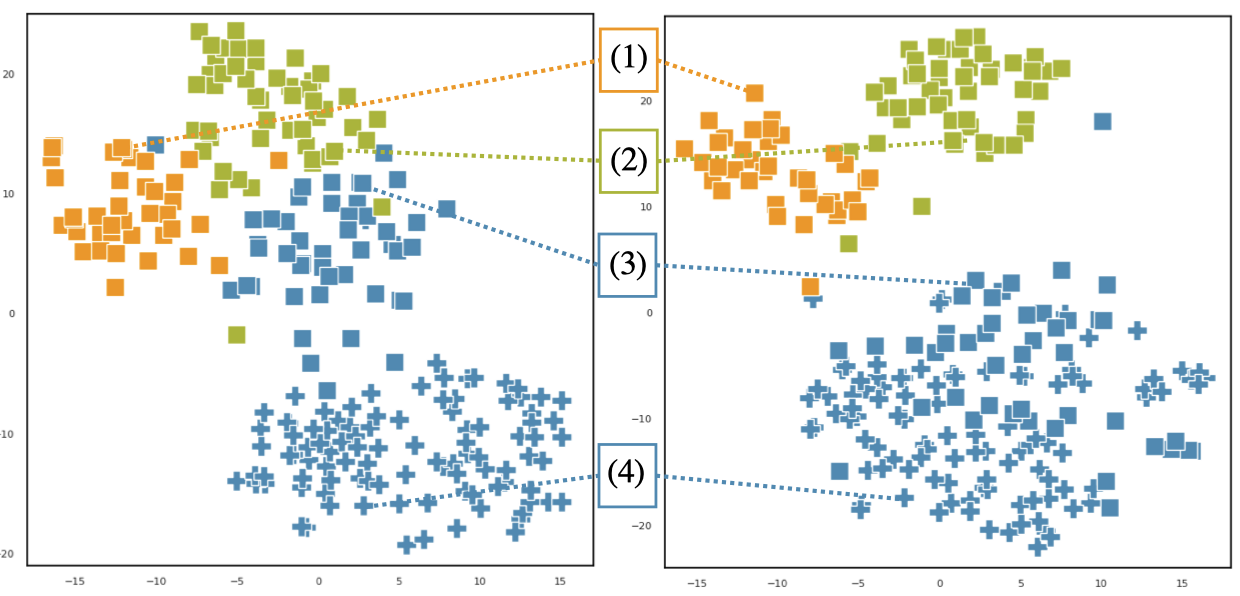
\includegraphics[width=\textwidth]{figures/media/image7.png}
  \caption{\label{fig:bert}Figure 1 aus Yamada et al. \autocite*[811]{yamadaSemanticFrameInduction2021}. Originale Bildunterschrift: \emph{2D projections of BERT embeddings of verbs (left) and masked verbs (right). Numbers in the figure correspond to numbers in Table 1,} ⬛ \emph{and \textbf{+} are verbs ``get'' and ``acquire'', respectively, and each color indicates \textcolor[RGB]{234,151,44}{ARRIVING}, \textcolor[RGB]{170,181,61}{TRANSITION\_TO\_STATE}, and \textcolor[RGB]{81,137,177}{GETTING} frame.}}
\end{figure}

Mithilfe des Language Models BERT \autocite{devlinBERTPretrainingDeep2019} können sie für jedes Verb in diesen Sätzen eine kontextualisierte Vektor-Repräsentation erzeugen. Im Gegensatz zu klassischen Word Embeddings (\chapref{word-embeddings-als-paradigmatische-distributionelle-muster}) erhalten sie so ein Embedding pro Token und nicht pro Type und können unterschiedliche Verbbedeutungen und mithin unterschiedliche LE potenziell unterscheiden. \figref{fig:bert} zeigt die Verbesserung, die sie erreichen, indem sie BERT das Embedding nicht für das Verb-Token, wie es im Satz steht, erzeugen lassen, sondern es zuvor maskieren, sodass das Sprachmodell keine Information darüber erhält, welches Wort an der Stelle eigentlich steht. Es wird also z.\,B. ein Embedding für die maskierte Stelle im Satz \emph{We'll not} {[}MASK{]} \emph{there before the rain comes} erzeugt. Dem linken Teil der Abbildung ist zu entnehmen, dass in der unmaskierten Variante die Sätze mit den drei Bedeutungen von \emph{get} zwar bereits in unterschiedlichen Clustern zu finden sind, allerdings jeweils durch die identische Formseite auch einander äußerst nah sind. Erst durch die Maskierung, deren Ergebnisse im rechten Teil der Abbildung dargestellt sind, sind Sätze mit \emph{get} in der GETTING-Bedeutung deutlicher separiert und bilden -- zielgemäß -- ein gemeinsames Cluster mit den Sätzen mit \emph{acquire} in der GETTING-Bedeutung. Es liegen des Weiteren Ansätze vor, die FE induzieren und grundsätzlich ähnlich funktionieren, wobei aber auch syntaktische Dependenzbeziehungen der Verben zu ihren Argumenten einbezogen werden \autocite[z.\,B.][]{anwarHHMMSemEval2019Task2019}.

Word Embeddings beruhen auf paradigmatischer distributioneller Ähnlichkeit, d.\,h. Wörter mit ähnlichen Kotexten erhalten ähnliche Vektorrepräsentationen und sind mithin in gleichen Clustern zu finden. Die Embedding-basierten Ansätze zur Frame-Induktion greifen also auf distributionelle Eigenschaften von Sprache zurück, um sie Frames zuzuordnen. Gemäß der Ausrichtung von \emph{FrameNet} sind auch die Frame-induzierenden Ansätze in aller Regel an Verben interessiert und teilen mithin das Defizit der Fillmoreschen Frame-Semantik, den konzeptuellen Gehalt von (u.\,a.) Nomen und Adjektiven zu vernachlässigen (\chapref{welche-frames-werden-aufgenommen} und \ref{warum-frames}). Auch beschränken sie sich weitestgehend auf die Zuordnung von Verben zu bestehenden \emph{FrameNet}-Frames, anstatt wirklich neue Frames zu erschließen und deren FE zu beschreiben.

\subsection{Distributionell-semantische Methodik}\label{distributionell-semantische-methodik}

In korpuslinguistischen Zugängen hat sich eine Reihe distributioneller Methoden etabliert, um die Semantik sprachlicher Einheiten von der Wort- bis zur Textebene zu erfassen. Die wohl etabliertesten und insbesondere auch im Bereich der englischsprachigen CADS viel genutzten Verfahren sind die Kollokations- und die Keyword-Analyse.\footnote{Siehe dazu etwa Gillings et al. (2023: 2), die diese zusammen mit Frequenz- und Konkordanz-Analyse als „the four main corpus tools`` listen.} Die Idee der Kollokationsanalyse ist in \chapref{distributionelle-semantik} bereits umrissen worden und wird in \chapref{kollokationen-als-syntagmatische-distributionelle-muster} näher in ihrer Funktionsweise erläutert. Es geht bei ihr darum, die Semantik eines Wortes und seine Gebrauchsprofile in einzelnen Diskursen über das statistisch signifikant häufige Ko-Vorkommen mit anderen Wörtern zu erschließen. Zur Messung der statistischen Signifikanz können dabei unterschiedliche Maße zum Einsatz kommen, die je unterschiedliche Ergebnisse produzieren (siehe \chapref{wie-funktioniert-die-berechnung-von-kollokationen}). Baker etwa stellt in Bezug auf vorherige Untersuchungsergebnisse \autocite{bakerDiscourseAnalysisMedia2013} heraus, dass das Adjektiv \emph{muslim} in der britischen Presse insbesondere in Bezug auf islamistische Akteure genutzt wird:

\begin{quote}
We found that one common pattern in this context concerned words relating to extreme belief, such as \emph{extremist}(\emph{s}), \emph{fundamentalist}(\emph{s}) and \emph{militant}(\emph{s}). Such words also were common when Muslim was a noun, and they also occurred frequently with two other high-frequency words \emph{Islam} and \emph{Islamic}. \autocite[248]{bakerAcceptableBiasUsing2012}
\end{quote}

In einer vertiefenden Analyse zeigt er außerdem, dass sie weitaus häufiger gebraucht werden als Wörter, die einen strengen, aber nicht extremistischen oder moderaten Glauben anzeigen (Baker 2012: 251--252), was auf einer in diesen Ansätzen häufig vorgenommenen Kategorisierung der Kollokate nach semantischen Gesichtspunkten beruht. Zur Analyse von Framing arbeiten auch Czulo et al. \autocite*{czuloEinflussExtremistischerGewaltereignisse2020} mit Kollokationen (siehe \chapref{weitere-arbeiten-zum-extremismusdiskurs-und--begriff}). Für eine Übersicht über die zahllosen weiteren Anwendungen von Kollokationsanalysen sei auf den ausführlichen Literaturüberblick bei Storjohann \autocite*{storjohannKookkurrenzAusKorpuslinguistischer2016} verwiesen.

In Bezug auf methodologische Weiterentwicklungen ist die besonders raffinierte Version der Kollokations-Analyse von Belica zu nennen. Sie ist über die Kookkurrenzdatenbank CCDB am IDS-Mannheim \autocite{belicaKookkurrenzdatenbankCCDBKorpuslinguistische2001} zugänglich und listet neben den unmittelbaren Kollokaten rekursiv auch deren Kollokate sowie typische syntagmatische Muster. Für die Analyse von Konstruktions-Fillern in der Konstruktionsgrammatik ist die von Stefanowitsch \& Gries \autocite*{stefanowitschCollostructionsInvestigatingInteraction2003} entwickelte und ebenfalls auf Kollokationen beruhende Kollostruktionsanalyse einschlägig, mit deren Hilfe sich etwa \emph{give}, \emph{tell} und \emph{send} als typische Filler des Verb-Slots der \emph{ditransitive construction} identifizieren lassen \autocite[229, Table 10]{stefanowitschCollostructionsInvestigatingInteraction2003}, was gemäß distributionell-semantischer Annahmen eine wichtige Dimension von Konstruktionsbedeutungen darstellt \autocite{ziemDimensionsConstructionalMeanings2023}. Eine andere Weiterentwicklung stellt die Berechnung und Visualisierung ganzer Kollokationsnetzwerke dar, in denen auch gegenseitige Abhängigkeiten der Kollokate eines Wortes in Form eines Netzwerk-Graphen dargestellt sind. Brezina et al. heben zum einen ihren zusammenfassenden Charakter und den Zugang zur „psychological notion of the `aboutness' of a text`` \autocite*[142]{brezinaCollocationsContextNew2015} im Sinne von Phillips \autocite*{phillipsLexicalStructureText1989} hervor, gehen aber auch auf ihr Potenzial ein, komplexe diskursive Bedeutungszusammenhänge zu erkennen, u.\,a. am Beispiel des \emph{swearing discourse}:

\begin{quote}
To appreciate the complexity of the moralistic discourse we also need to look at how the immediate associations are connected with one another and, more importantly, how these are connected to other (more distant) associations. Thus, for instance, in 17th and 18th century discourse, \emph{swearing} is connected with a whole range of religious evaluations, through further associations of vice with notions such as \emph{prophaneness} and \emph{irreligion} {[}\ldots{]}. Ultimately, any discourse rests upon a large network of associations, where each one activates a number of others (cf. Hoey 2005), that produces social meaning through multiple cross-associations. These cross-associations, however, cannot be observed even with careful reading of source documents, but need to be analysed using a tool that allows simultaneous multiple comparisons of word frequencies and co-occurrences. \autocite[155]{brezinaCollocationsContextNew2015}
\end{quote}

Die Visualisierung hat darüber hinaus auch schlicht den Vorteil, eine lange Liste von Kollokationsbeziehungen in einem Korpus überhaupt überblicken zu können:

\begin{quote}
Es ist unmöglich, durch Lesen solcher langer Listen einen Eindruck über das Ensemble der Verknüpfungen zu erhalten. Erst durch die Visualisierung als Netz kann sich ein Bild ergeben (Pfeffer 2010; für einen historischen Blick auf Visualisierungen von Netzwerken: Kruja et al. 2002). \autocite[231]{bubenhofer9DiskurslinguistikUnd2018}
\end{quote}

Letztlich sei auf Bakers Arbeit verwiesen, die das Potenzial von Kollokationsnetzwerken hervorhebt, u.\,a. bedeutungsäquivalente Wörter zu erkennen, und zwar dadurch dass sie ähnliche Kollokate aufweisen, ohne zwingend gemeinsam aufzutreten \autocite*[147-148]{bakerShapesCollocation2016} -- ein Befund also, der sich vor dem Hintergrund distributionell-semantischer Annahmen bestens erklären lässt und auch der Idee von Word Embeddings (s.u.) zugrundeliegt.

Keyword-Analysen (dt. auch Schlüssel- oder Schlagwortanalysen) sind im Gegensatz zu Kollokationsanalysen eine \emph{corpus-driven} und kontrastive Methode, die Wörter\footnote{Statt einzelner Wörter können natürlich auch Mehrworteinheiten bzw. Sprachgebrauchsmuster oder einzelne Annotationen in Hinblick auf ihre Keyness bewertet werden \autocite{bubenhoferSprachgebrauchsmusterKorpuslinguistikAls2009, bubenhofer4KollokationenNGramme2017}.} zu Tage fördert, die in einem Korpus signifikant häufiger gebraucht werden als in einem anderen Korpus. Sie dienen so dazu, die \emph{aboutness} eines Korpus zu erschließen \autocite{gabrielatosKeynessAnalysisNature2018} und wurden auch bereits bei der Analyse von kommunikationswissenschatlichem Framing \autocite{bakerChangingFramesObesity2020} sowie in Frame-semantischen Ansätzen \autocite{ziemMedienFramesAlsSemantische2018} eingesetzt. Eine Nutzung von Keywords als Features in multiplen Korrespondenzanalysen wurde von Clarke et al. vorgeschlagen \autocite{clarkeMultipleCorrespondenceAnalysis2021, clarkeKeywordsTimeTracking2022}. Während bei der Kontrastierung nach z.\,B. diachronen oder akteursbezogenen Kriterien\footnote{Nur beispielhaft genannt seien Bubenhofer \autocite*{bubenhofer4KollokationenNGramme2017}, der den Nutzen der Methode zur Analyse des typischen Wortschatzes einzelner Parteien vorführt und Clarke et al. \autocite*{clarkeKeywordsTimeTracking2022}, die diachrone Unterschiede im Islamdiskurs fokussieren.} unstrittige Metadaten zur Bildung der zu vergleichenden Korpora genutzt werden können, erfordert der Vergleich einzelner thematischer Diskurse die voraussetzungsreichere Bildung entsprechender virtueller Diskurskorpora \autocite{busseIstDiskursSprachwissenschaftliches1994}. Dies geschieht in der Korpuslinguistik zumeist durch die Festlegung einzelner repräsentativer Suchwörter, wobei nur die Texte, die diese Wörter enthalten, in das Korpus aufgenommen werden. Dieser Schritt ist jedoch durchaus kritisch, da so -- Frame-semantisch gesprochen -- bereits vorausgesetzt wird, welche LE einen thematischen Frame evozieren. Genau das soll ja aber auch das Ergebnis der Analyse sein. So könnte, wer ein Diskurskorpus zum Islamismus zusammenstellt und dafür das Lemma \emph{islamistisch} verwendet, Texte verpassen, in denen -- wie diskurslinguistisch bereits mehrfach herausgestellt -- regelmäßig nicht von ‚Islamisten`, sondern z.\,B. \emph{muslimischen Extremisten} \autocite[116, Tabelle 23]{kalwaKonzeptIslamDiskurslinguistische2013} oder \emph{fanatic Muslims} \autocite[249, Table 1]{bakerAcceptableBiasUsing2012} die Rede ist. Natürlich ist es wahrscheinlich, dass in vielen Texten, in denen von \emph{muslimischen Extremisten} die Rede ist, \emph{auch} das Wort \emph{islamistisch} vorkommt, was das Problem deutlich mindert. Und auch bei der Untersuchung thematisch eng gefasster Diskurse wie der Snowden-Affäre \autocite{ziemMedienFramesAlsSemantische2018} oder der frühen Corona-Pandemie \autocite{bubenhoferGrenzenUndWelten2020} ist es unwahrscheinlich, dass die zugrundegelegten \emph{seed words} (\emph{Snowden}, \emph{NSA}, \emph{data} bzw. \emph{Corona}) nicht in den Texten vorkommen. Für den in der vorliegenden Arbeit zu untersuchenden Extremismus-Diskurs, bei dem begriffliche Verwirrungen und Unsicherheiten fortwährender Gegenstand der wissenschaftlichen Debatte sind und für den im Untersuchungszeitraum eine geradezu unzählige Menge relevanter Ereignisse und Akteure zu berücksichtigen gelten würde, kommt ein solches Vorgehen und mithin Keyword-Analysen nicht in Frage. Stattdessen soll nach Möglichkeiten gesucht werden, auch in einem thematisch heterogenen Korpus einzelne Diskurse bzw. thematische Frames datengeleitet aufzuspüren.

Neben diesen etablierten Methoden haben auch neuere, aus der Computerlinguistik stammende Verfahren Anwendung in diskursanalytischen Arbeiten gefunden. Zum einen ist hier Topic Modelling \autocite{bleiLatentDirichletAllocation2003} zu nennen, mit dessen Hilfe für jedes Wort und jeden Text (\emph{document}) in einem Korpus bestimmt werden kann, mit welcher Wahrscheinlichkeit es zu einem \emph{topic} gehört. Zugrunde liegt ebenfalls die Verteilung von Wörtern über die \emph{documents} des Korpus, wobei jedes einzelne \emph{document} als sogenannte \emph{bag of words} aufgefasst wird, sodass die syntagmatische Nähe bzw. Abfolge der Wörter keine Rolle spielt. Die \emph{topics} werden durch Listen von Wörtern dargestellt. So finden etwa Bubenhofer et al. \autocite*[82]{bubenhoferDigitaleKulturlinguistikDigitalitaet2022} in Rezepten der Plattform Chefkoch ein \emph{topic} mit Wörtern wie \emph{leider}, \emph{zwar}, \emph{überhaupt} und \emph{irgendwie}, das sie als Bewertungen und Positionierungen interpretieren. Weiterhin angewendet wurde Topic Modeling in der Diskurslinguistik z.\,B. bei Törnberg \& Törnberg \autocite*{tornbergMuslimsSocialMedia2016}, Murakami et al. \autocite*{murakamiWhatThisCorpus2017}, Bubenhofer et al. \autocite*{bubenhoferGrenzenUndWelten2020} oder Dreesen et al. \autocite*{dreesenOperationalisierungDiskurslinguistischenKategorie2023}; kritisch reflektiert in den Arbeiten von Brookes \& McEnery \autocite*{brookesUtilityTopicModelling2019} sowie Gillings \& Hardie \autocite*{gillingsInterpretationTopicModels2023}. Da Topic Modeling durchaus interessante Möglichkeiten für \emph{corpus-driven} Ansätze eröffnet, wurde auch bei der Methodenentwicklung in diesem Projekt mit dem Verfahren experimentiert; die Anforderungen an den Arbeitsspeicher überstiegen jedoch aufgrund des sehr großen Korpus die zur Verfügung stehenden Möglichkeiten. Des Weiteren liegt das eigentliche Ziel des Verfahrens, die thematische Klassifikation von Texten, nicht im Untersuchungsinteresse; die Modellierung und das Clustering einzelner Wortbedeutungen wiederum ist hingegen besser durch die computerlinguistische Methodengruppe der Word Embeddings zu realisieren.

Wie bereits erwähnt, ist es mithilfe von Word-Embedding-Algorithmen möglich, Wörter auf der Grundlage ihrer Distribution in Korpora in Vektoren zu überführen. Die Nähe und Distanz im sich ergebenden Vektorraum entspricht dabei einer paradigmatischen distributionellen Ähnlichkeit; benachbarte Wörter haben ähnliche Kotexte (siehe ausführlicher \chapref{distributionelle-semantik} und \ref{word-embeddings-als-paradigmatische-distributionelle-muster}). Große Popularität gewonnen haben solche Ansätze mit der Verbreitung der Nutzung neuronaler Netze, die die ressourceneffiziente Berechnung von Word Embeddings für große Korpora erlaubte \autocite{mikolovEfficientEstimationWord2013}. In der Diskurslinguistik spielt bislang insbesondere die Analyse lokaler Nachbarschaften im Vektorraum eine Rolle, die semantisch-funktionale Äquivalenz widerspiegelt \autocite{bubenhoferSemantischeAquivalenzGeburtserzahlungen2020}. In diesem Rahmen können auch Clustering-Algorithmen wie \emph{k-Means} \autocite{macqueenMethodsClassificationAnalysis1967} zum Einsatz kommen, die solche Nachbarschaften automatisiert erkennen (siehe \chapref{clustering-von-word-embeddings}). Bubenhofer zeigt so etwa, dass ein Wort-Cluster um die (Mehrwort\mbox{-})Lemmata \emph{demokratisch Staat}, \emph{zentralistisch} und \emph{totalitär Regime} während der Corona-Pandemie deutlich häufiger durch rechte und Corona-skeptische Medien wie u.\,a. Compact Online und KenFM.de gebraucht wurde:

\begin{quote}
Die Verteilung über die Quellen in Abbildung 2 zeigt nun deutlich, dass Ausdrücke des Clusters in den Skep-Medien deutlich häufiger verwendet werden. Die Kommentare (mit Ausnahme von 20 Minuten) liegen zusammen mit den CH-Medien NZZ und Tages-Anzeiger dazwischen. In den restlichen Quellen werden die Ausdrücke des Clusters seltener verwendet. Es muss berücksichtigt werden, dass mit \emph{demokratisch} und \emph{regieren} zwei Ausdrücke im Cluster vorhanden sind, die hinsichtlich eines politischen Standpunktes (in einer Demokratie) unauffällig sind. Die meisten der restlichen Ausdrücke jedoch sind Stigmawörter (Spitzmüller/ Warnke 2011, S. 143) und kritisieren im Kontext der Corona-Pandemie die angeblich totalitäre Ausrichtung des Staates. {[}\ldots{]} Auch die Cluster 843 (\emph{Diktatur}, \emph{Polizeistaat}, \emph{totalitär Staat}) und 1731 (\emph{Ungehorsam}, \emph{Gesundheitsdiktatur}, \emph{Repression}) enthalten Stigmawörter für den Staat und werden in den Skep-Medien häufiger verwendet als in den anderen Quellen. \autocite[205-206]{bubenhoferExplorationSemantischerRaeume2022}
\end{quote}

Das Clustering und die Analyse der Frequenz-Unterschiede in unterschiedlichen Medien können also ohne die Notwendigkeit von händischen Annotationen Charakteristika des Sprachgebrauchs einzelner medialer Akteure freilegen. Weiterhin analysiert Bubenhofer, wie zuvor in Zusammenarbeit mit Calleri und Dreesen \autocite*{bubenhoferPolitisierungRechtspopulistischenMedien2019}, divergierende Semantisierungen einzelner Wörter im Vergleich der Korpora. Da die Vektoren von auf unterschiedlichen Korpora berechneten Word-Embedding-Modellen nicht unmittelbar vergleichbar sind (siehe \chapref{vergleichbarkeit-von-word-embedding-modellen}), werden dabei nicht die Vektoren selbst verglichen, sondern ihre lexikalischen Nachbarn im Vektorraum. Einen deutlichen Unterschied stellt er u.\,a. beim Ausdruck \emph{Narrativ} fest:

\begin{quote}
In den beiden Modellen sind nur \emph{Halbwahrheit}, \emph{instrumentalisiert}, \emph{Massenmedium}, \emph{Populismus} und \emph{Verschwörung} semantisch ähnliche Ausdrücke, die in beiden Modellen vorkommen. Ansonsten unterscheiden sich die Modelle deutlich. Nächste Nachbarn wie \emph{Angsterzeugung}, \emph{aufbauschen}, \emph{böse Absicht}, \emph{dahinter stecken}, \emph{Fiktion}, \emph{infam}, \emph{Inszenierung}, \emph{krampfhaft}, \emph{Leugnung}, \emph{Lügenpropaganda}, \emph{Massenpsychologie}, \emph{psychologische} Kriegsführung, \emph{Unwahrheit}, \emph{Wahn} oder \emph{Weltverschwörung} zeichnen einen semantischen Raum, bei dem \emph{Narrativ} als bösartige Manipulation semantisiert ist. Im CH-Medien-Korpus gibt es ebenfalls Ausdrücke, die diese Semantisierung nahelegen, jedoch auch andere wie \emph{westliche Demokratie}, \emph{Ideologie}, \emph{Deutungshoheit} oder \emph{politische Debatte}, die der sozialwissenschaftlichen Definition von Narrativ als sinnstiftende Erzählung näher kommen (Lyotard 2015). \autocite[214]{bubenhoferExplorationSemantischerRaeume2022}
\end{quote}

Dass in Word Embeddings weit mehr als eine globale semantisch-funktionale Ähnlichkeit gespeichert ist, zeigen Kozlowski et al. \autocite*{kozlowskiGeometryCultureAnalyzing2019}. In einer aufwändigen diskursanalytischen Untersuchung zum Konzept \emph{class} nutzen sie Antonympaare wie \emph{poor} und \emph{rich} oder \emph{masculine} und \emph{feminine}, um semantische Achsen im Vektorraum aufzuspannen. Sie können so unterschiedliche in der Literatur beschriebene Dimensionen des Konzeptes wie ‚Wohlstand`, ‚\emph{race}` oder ‚Gender` operationalisieren und diachrone diskursive Veränderungen vermessen. \figref{fig:kozlowski} zeigt exemplarisch, wie so einzelne Sportarten in Hinblick auf diese Dimensionen verortet werden können. Dass solche vektorgeometrischen Berechnungen nicht nur dem Anschein nach plausibel Auskunft über in Diskursen manifestierte Stereotype geben, sondern tatsächlich eng mit Sprecher*innen-Urteilen korrelieren, belegen sie durch eine Fragebogenstudie \autocite[siehe auch aus kognitionswissenschaftler Perspektive][]{grandSemanticProjectionRecovers2022}.

\largerpage
\begin{figure}[b]
\includegraphics[width=.7\textwidth]{figures/media/kozlowski-cropped.png}
  \caption{\label{fig:kozlowski}Semantische Projektion der Wortvektoren unterschiedlicher Sportarten auf zwei ‚kulturelle Dimensionen` (eigene Visualisierung von \emph{Figure} 2c aus \citealt[913]{kozlowskiGeometryCultureAnalyzing2019}).}
\end{figure}

Für kulturwissenschaftliche Fragestellungen bedeutet dies nicht weniger als die Möglichkeit, die Intersektionalität unterschiedlicher kultureller Dimensionen modellieren zu können:

\newpage
\begin{quote}
The ability of word embedding models to simultaneously locate objects on multiple cultural dimensions, including race, gender, class, and many others, makes them a powerful tool for studies of intersectionality. The fundamental insight of the intersectionality literature is that cultural categories, particularly those of identity, cannot be isolated and understood independently (Crenshaw 1991; McCall 2005). Rather, analysts must always consider ways in which the meanings of cultural categories change as they overlap and intersect one another. Interrogation of the intersection of cultural categories becomes empirically tractable through word embedding models. For example, comparing words that project high on both affluence and masculinity to those that project high on affluence and femininity will reveal how markers of class differ across gender lines within the cultural world in which the texts were produced. The theory that identity is defined by numerous crosscutting and overlapping categories is itself predicated on a ``high-dimensional'' model of culture similar to that modeled by Euclidean word embeddings. Indeed, the empirical success of word embedding models to represent cultural dimensions promotes a radical view of intersectional identity, modeled not as a low-dimensional matrix, but rather a highdimensional array composed of hundreds or thousands of interacting cultural associations. \autocite[914-915]{kozlowskiGeometryCultureAnalyzing2019}
\end{quote}

Auch linguistische Ansätze, in denen einzelne sprachliche Einheiten semantisch gruppiert werden sollen, profitieren von der Möglichkeit einer induktiven und hochdimensionalen Modellierung von Wortbedeutungen. So weiß jede*r, der*die entsprechende Annotationen schon einmal händisch durchgeführt hat, dass man ständig Zweifelsfällen begegnet, in denen ein Wort -- womöglich in Abhängigkeit des konkreten jeweiligen Kontextes -- in verschiedene Kategorien gezählt werden könnte. Letztlich ist man jedoch, um die Komplexität beherrschbar zu halten und auch um ein Agreement mit den anderen Annotator*innen zu erreichen, i.d.R. gezwungen, sich auf eine Möglichkeit festzulegen. Es wäre ja andernfalls auch notwendig, die Zugehörigkeit zu den unterschiedlichen Kategorien graduell zu quantifizieren, was nur noch in sehr kleinen Untersuchungen zu leisten wäre. Ein Beispiel stellt die Untersuchung von Baker et al. (2020) dar. Sie berichten zunächst, dass sie sich gegen den Einsatz eines (durchaus verbreiteten) semantischen Taggers wie \emph{Wmatrix} \autocite{raysonKeyWordsKey2008} entschieden haben, der Wörter im Wesentlich auf Basis eines statischen Thesaurus in Kategorien einordnet. Stattdessen, insbesondere um kontextuelle Faktoren besser berücksichtigen zu können, entscheiden sie sich für eine induktive manuelle Kategorisierung von Keywords:

\begin{quote}
Automatic taggers do not always recognise every word they encounter and often assign categories based on surface meaning, whereas it can be more useful to take into account the contexts in which the words are used. For example, one of the categories we created was ILLNESS, which contained words like \emph{cancer}, \emph{diabetes} and \emph{inflammation}. We included words like~\emph{heart}~and~\emph{liver}~in this category, as our explorations of how those words occurred in the context of articles revealed that they almost always referred to heart or liver disease. However, we did not categorise the word~\emph{epidemic}~as ILLNESS, as instead we found it was almost always used metaphorically to refer to purported increases in rates of obesity, for example:

\begin{quote}
High~sugar consumption~is said to be fuelling the obesity epidemic, which is leading to increased cases of~heart disease. (\emph{Daily Mail}, April 2009)
\end{quote}

Thus, we created a category called PROBLEM and included~\emph{epidemic}~alongside words such as~\emph{risk},~\emph{crisis}~and~\emph{problem}, as all four words were used to frame obesity in a negative way. Categorisation was carried out separately by two of the authors at first and then jointly to resolve a small number of disagreements. We should note that we did not speculate about how the keywords in our data were used in order to categorise them. Rather, we closely analysed at least 100 random cases of each of the words to resolve them into categories that best reflected their most typical use (this was a method first adopted in Baker et al. (2019), based on experimenting with different numbers of cases in order to identify an amount which was most effective at identifying the range of contexts that a word can occur in). Where a word had more than one meaning and could appear in multiple categories, we chose the meaning which was most frequent out of the 100 random cases examined. Not all words could be easily assigned to a category as they had a range of frequent meanings or were used in ambiguous ways. For this reason, we did not categorise 131 of the keywords. \autocite[4]{bakerChangingFramesObesity2020}
\end{quote}

Hier ist m.\,E. durchaus fraglich, warum die als Beispiel angeführte „obesity pandemic`` nicht sowohl einen semantischen Bezug zum Bereich „PROBLEM`` als auch zum Bereich „ILLNESS`` aufweisen sollte. Und auch das Ansinnen, in einem aufwändigen Verfahren dominante Bedeutungen von Wörtern aus Konkordanzsamples zu erschließen, um eindeutige Annotationen vornehmen zu können bzw. ambige Wörter dabei auszuschließen, wird der tatsächlichen Komplexität von Semantik m.\,E. nicht gerecht. Natürlich kann der Schritt aus forschungspraktischen Gründen vollkommen gerechtfertigt sein und keine Untersuchung kommt ohne Vereinfachungen aus -- umso potenzialreicher erscheint jedoch die Möglichkeit einer hochdimensionalen Bedeutungsmodellierung mithilfe von Word Embeddings. So resümieren auch Kozlowski et al.:

\begin{quote}
The very success of these models provides suggestive validation for relational approaches to cultural theorizing. Furthermore, by operationalizing a high dimensional model of culture, word embedding models allow researchers to extend and contend with theories of culture in novel ways. Embeddings present a much vaster set of potential axes along which individuals and social groups may compete, cooperate, fracture, or coalesce than low-dimension theories of cultural constraint allow. By simultaneously capturing the multiplicity of associations expressed in language, word embedding models are able to represent a complex geometry of culture, which, like a many-faceted crystal, amplifies the subtle and shifting framings that enable coordinated and spontaneous social action. \autocite[931]{kozlowskiGeometryCultureAnalyzing2019}
\end{quote}

Eine Kombination von syntagmatischen und paradigmatischen Methoden für diskurssemantische Fragestellungen schlagen Vachková \& Belica \autocite*{vachkovaSelfOrganizingLexicalFeature2008} unter Nutzung der von Belica \autocite*{belicaKookkurrenzdatenbankCCDBKorpuslinguistische2001, belicaSemantischeNaheAls2011} für die Linguistik adaptierten Methode der s\emph{elf-organizing lexical feature maps} \autocite[SOM;][]{kohonenSelfOrganizingMaps2001} vor. Dabei wird die syntagmatische Kollokationsanalyse mit einer paradigmatischen Analyse geteilter Kollokationsprofile der Kollokate gepaart. \figref{fig:som-tod} zeigt ein Beispiel.

\begin{figure}[t]
  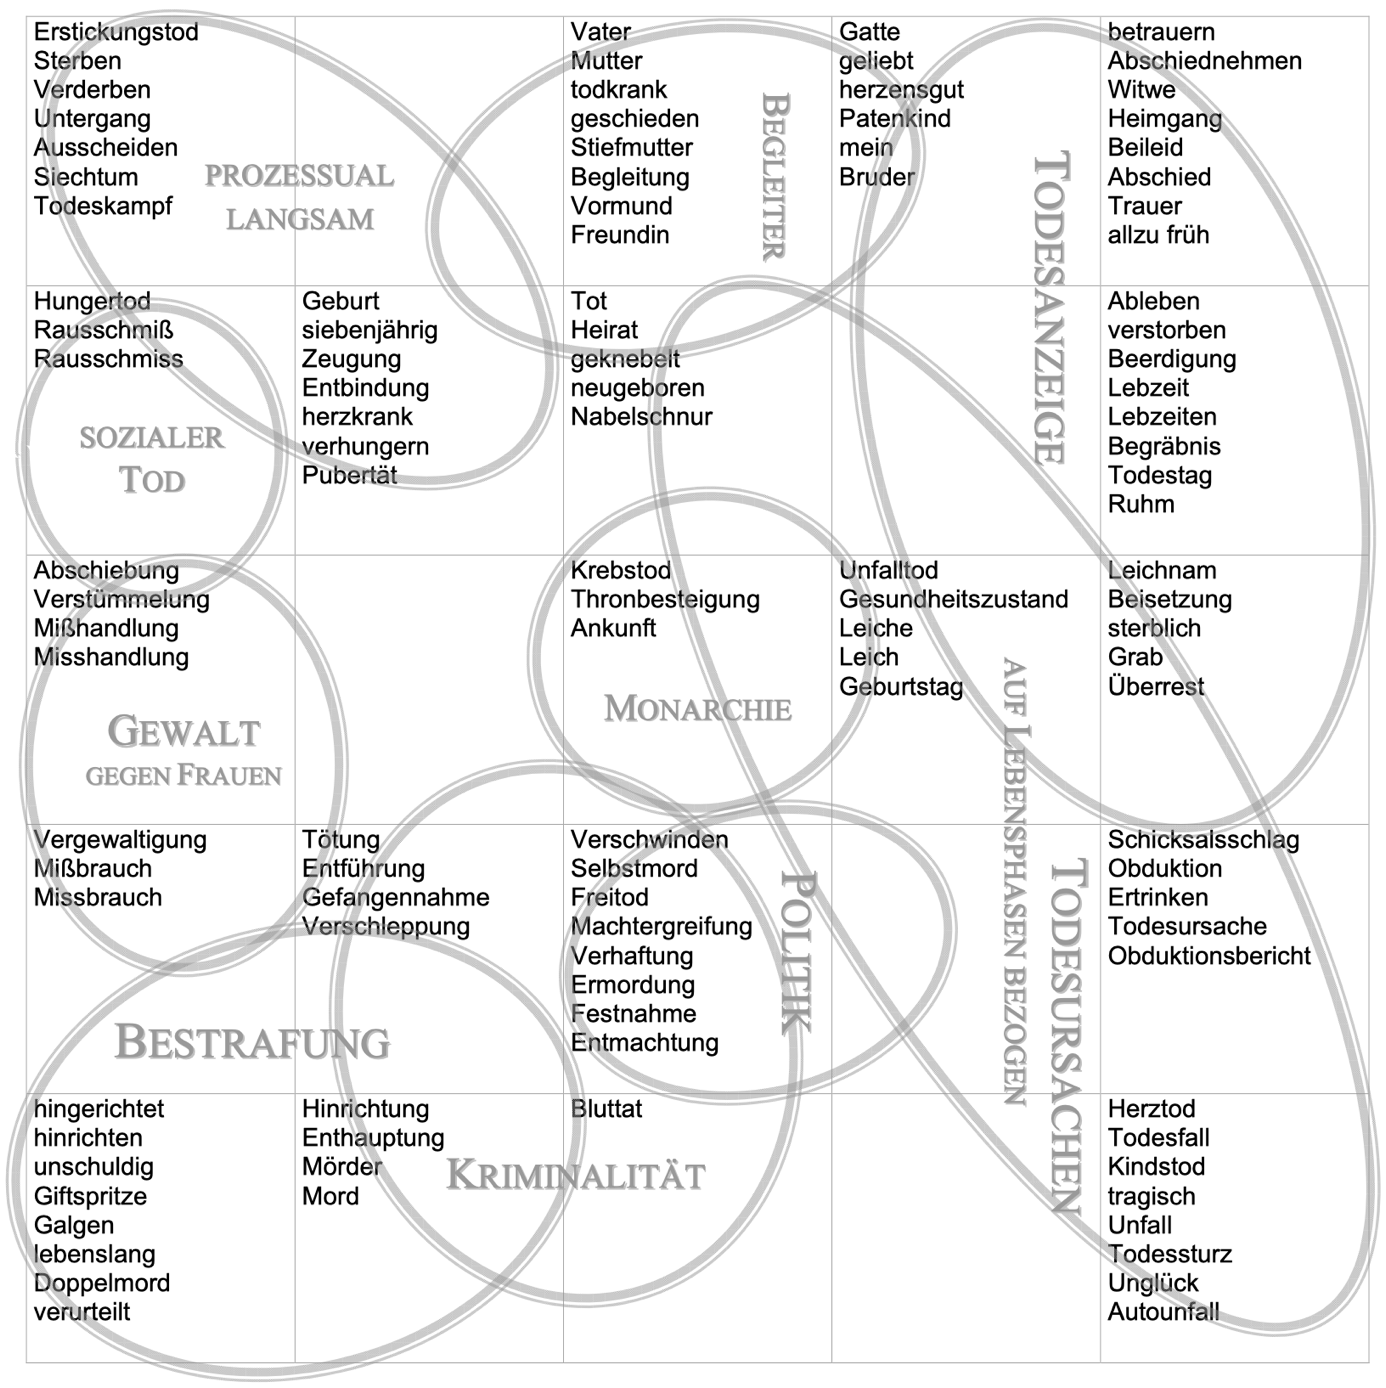
\includegraphics[width=\textwidth]{figures/media/image9.png}
  \caption{\label{fig:som-tod}Annotierte SOM zu \emph{Tod} (\emph{Figure 3} aus \citealt[250-251]{vachkovaSelfOrganizingLexicalFeature2008}).}
\end{figure}

In den einzelnen Quadraten sind jeweils Kollokate zum Wort \emph{Tod} dargestellt. Die Kollokate werden jedoch zusätzlich geclustert, sodass Kollokate, die selbst wiederum ähnliche Kollokationsprofile aufweisen, miteinander in einem Quadrat zu finden sind. Die sich ergebenden Cluster sind sodann interpretierbar und zeigen etwa den Trauer-Aspekt von Tod (u.\,a. \emph{betrauern}, \emph{Abschiednehmen}, \emph{Witwe}) oder den Kriminalitäts- bzw. Bestrafungs-Aspekt in jeweils grausamer Ausprägung an (u.\,a. \emph{Bluttat}, \emph{Hinrichtung}, \emph{Enthauptung}). Die Autor*innen konstatieren:

\begin{quote}
We suggest that the proposed approach of self-organizing clustering of collocation profiles extracted from very large text corpora followed by a discourse-based semiotic interpretation and a deferred mapping of the emergent signs to systemic linguistic categories is a coherent and adequate methodology for the explorative study of language. We argue that the epistemic results obtained by applying this methodology also entail predictive and explanatory power. \autocite[238-239]{vachkovaSelfOrganizingLexicalFeature2008}
\end{quote}

Fragt man in der CCDB die SOM zum Lemma \emph{Extremismus} ab, findet sich einerseits ein Cluster wie {[}\emph{Nährboden}, \emph{Separatismus}, \emph{Terror}, \emph{Anwachs}, \emph{Anwachsen}, \emph{Gedankengut}, \emph{rassistisch}, \emph{Hetze}{]}, das die ideologische, im Verborgenen anwachsende Gefahr von extremistischem Gedankengut anzeigt; andererseits ein Cluster wie {[}\emph{Rassismus}, \emph{Fremdenfeindlichkeit}, \emph{Ausländerfeindlichkeit}, \emph{Fremdenhaß}, \emph{Fremdenhass}, \emph{Ausländerhaß}, \emph{Ausländerhass}, \emph{Ausgrenzung}{]}, das also Rassismus und Xenophobie, d.\,h. im Rechtsextremismus vorzufindende Einstellungen, zusammenfasst. Diese Beobachtung ist von großem Interesse für das Vorhaben einer korpuslinguistischen Untersuchung des Extremismusdiskurses, zeigen sich hier doch wesentliche semantische Dimensionen von Extremismus, die auch als FE eines Extremismus-Frames interpretierbar sind. So bündelt das zweitgenannte Cluster Einstellungen bzw. Motivationen rechtsextremistischer Akteure und enthält zugleich LE, die dieses FE evozieren. Es zeichnen sich in einer solchen Kombination distributioneller Verfahren, die im Fall der SOM noch limitiert und auf die Analyse einer vorberechneten Menge von Lemmata begrenzt ist, also sehr vielversprechende Potenziale für eine korpuslinguistische Frame-Modellierung ab, die es weiter zu prüfen gilt.

\section{Resümee}\label{resuemee}

\subsection{Warum Frames?}\label{warum-frames}

Vor dem Hintergrund der dargelegten theoretischen Grundlagen soll im Folgenden noch einmal zusammengefasst werden, warum gerade Frames ein geeignetes Modell diskursiven Wissens darstellen, um diskursive Unterschiede im Framing von Extremismus zu analysieren. Es wird auch darauf eingegangen, warum dabei die Entscheidung für Busses Frame-Modell anstatt des verbreiteteren \emph{FrameNet}-Ansatzes getroffen wurde. Im Anschluss wird skizziert, warum distributionell-semantische Ansätze ein geeignetes Mittel sind, um Frames induktiv zu erschließen und welche genauen Verfahren für die sich anschließende Methodenentwicklung einbezogen werden. Letztlich sollen inhaltliche Mindestbestandteile eines Extremismus-Frames resümiert werden, um eine orientierende Grundlage für die datengeleitete Analyse zu schaffen.

Als Vorzug eines Frame-semantischen Modells für die Diskursanalyse ist erstens zu nennen, dass es die Bedeutungskomplexität einzelner Begriffe überhaupt erfassen und modellieren kann. So Busse zum Bereich der politischen Lexik:

\begin{quote}
Ein Wort wie \emph{Steuererleichterung} thematisiert das Leiden unter einer Last, \emph{Todessteuer} statt \emph{Erbschaftssteuer} evoziert „das unwillkommene Bild, für das Sterben bestraft zu werden`` und \emph{das kleine Baby} statt \emph{Fötus} evoziert die Assoziation „eines kleinen und hilflosen menschlichen Wesens, das des Schutzes bedarf`` (Fillmore 2006, 620). Solche Bedeutungselemente oder verstehensrelevanten Wissenselemente) können mit klassischen Mitteln und Modellen der linguistischen Semantik gar nicht erfasst werden. Gerade hier zeigt ein frame-analytisches Modell seine besondere Leistungsfähigkeit. Die politische Lexik kann daher als einer der idealen Gegenständer für einen frame-analytischen Ansatz in der Semantik angesehen werden. \autocite[198]{busse33LexikFrameanalytisch2017}
\end{quote}

Im Vergleich zu sozial- oder kulturwissenschaftlichen epistemologischen Modellen ist die Frame-Semantik außerdem von Beginn an auf die präzise Analyse der Wechselwirkung einzelner sprachlicher Zeichen mit diesen Wissensbeständen ausgerichtet. Dies betrifft sowohl die Möglichkeit, einen Frame im Sinne von Bezeichnungskonkurrenz mit unterschiedlichen Wörtern zu evozieren bzw. zu perspektivieren (siehe die Beispiele im obigen Zitat) als auch die kontrastive Erschließung von Bedeutungskonkurrenz, d.\,h. wenn mit demselben Ausdruck und in Abhängigkeit von z.\,B. einzelnen Akteuren unterschiedliche Frames oder Frame-Anteile evoziert werden (siehe zum strategischen Besetzen von Begriffen Klein 1991). Dass Frames nicht geeignet wären, multiple Verweismöglichkeiten von Ausdrücken auf Konzepte zu modellieren \autocite[13-14]{kalwaKonstitutionKonzeptenDiskursen2019}, trifft also nicht zu -- ganz im Gegenteil ist ja einer der zentralen Gedanken der Frame-Semantik, dass unterschiedliche Wörter den gleichen Frame evozieren und dabei jeweils unterschiedlich perspektivieren (siehe \chapref{entailment-case-grammar-understanding-semantics}). Letztlich ist auch die Visualisierbarkeit von Frames (üblicherweise als Netzwerk-Graph), gerade für explorative \emph{corpus-driven} Zugänge, ein nicht zu unterschätzendes Potenzial. Besonders wertvoll ist dies in kontrastiven Studien (wie der vorliegenden), die diachrone Bedeutungsveränderungen oder mediale Abhängigkeiten des Framings untersuchen, wie auch Busse hervorhebt:

\begin{quote}
Frame-analytische Verfahren und Darstellungsweisen sind nach meiner Auffassung besonders gut geeignet, um Fälle konkurrierenden Sprachgebrauchs zu kontrastieren und die semantischen Differenzen klar und deutlich herauszuarbeiten. Wegen derselben Eigenschaften eignen sie sich auch besonders gut zur Illustrierung von Bedeutungswandel. \autocite[210-211]{busse33LexikFrameanalytisch2017}
\end{quote}

Frame-semantische Modelle eignen sich außerdem hervorragend dazu, den Blick auch auf im Diskurs Ungesagtes zu richten, das in der Diskurslinguistik immer wieder als beachtenswert herausgestellt wurde \autocites[39]{spitzmullerDiskurslinguistikEinfuhrungTheorien2011}{storjohannPrasenzUndAbsenz2013}[sowie die Beiträge in][]{schroterExploringSilenceAbsence2018a}. Dies wird insbesondere sichtbar, wenn eigentlich vorgesehene Slots in einem Frame nicht (mehr) gefüllt werden. So formulieren Ziem et al., dass die ausbleibende Realisierung eines FE einem

\begin{quote}
induktiven Verfahren entgehen würde, da diesem zufolge Frame-Elemente allein auf der Basis des gegebenen sprachlichen Materials ermittelt werden. Gerade nicht realisierte Frame-Elemente können aber analytisch sehr interessant sein, insofern sie auf Wissensaspekte verweisen, die im Diskurs marginalisiert werden. \autocite[164]{ziemMedienFramesAlsSemantische2018}
\end{quote}

Einen Blick auf das Ungesagte kann m.\,E. allerdings nicht nur durch die Nutzung bestehender Ontologien wie \emph{FrameNet} gewonnen werden. Es sollte genauso möglich sein, über Kontrastierung unterschiedlicher induktiv gewonnener Frames entsprechende Leerstellen sichtbar zu machen. Einen ähnlichen Ansatz verfolgen auch Storjohann \& Schröter \autocite*{storjohannPrasenzUndAbsenz2013} und verweisen außerdem auf das Desiderat, Frame-Kategorien mithilfe „korpusgestützt{[}er{]} Analysen zahlreicher ähnlicher und nominaler oder verbaler Bezeichnungen`` \autocite*[206]{storjohannPrasenzUndAbsenz2013} aufzudecken. Dabei äußern sie auch den Bedarf einer korpuslinguistischen Methode, die „semantisch zusammenhängend{[}e{]} Kollokatoren und deren Kontexte nach unterschiedlichen linguistischen oder thematischen Kriterien bündeln`` \autocite[205]{storjohannPrasenzUndAbsenz2013} kann. Durch die Kombination von mithilfe von Word Embeddings semantisch gruppierten Wörtern, die als FE gelesen werden, und der Analyse der Kollokationen dieser Wort-Cluster wird die vorliegende Arbeit einen Beitrag zur Umsetzung des Desiderats leisten.

Letztlich ist zu rechtfertigen, warum die Entscheidung zugunsten Busses Frame-Modell, das laut Wengeler \autocite*[23]{wengelerWarnungVorFraming2022} in diskurs- und politolinguistischen Ansätzen kaum praktikabel sei, getroffen wurde, anstatt auf \emph{FrameNet} zurückzugreifen. Von der theoretischen Anlage her ist hier insbesondere der Fokus von \emph{FrameNet} auf Prädikationen zu nennen. Wie bereits in \chapref{welche-frames-werden-aufgenommen} erwähnt, sind zu fundamentalen und Diskurse der jüngeren Zeit bestimmenden Konzepten wie ‚Krieg`, ‚Frieden`, ‚Pandemie` oder eben ‚Extremismus` schlicht keine Frames verzeichnet.\footnote{Zwar ist es nachvollziehbar, dass in einer auf qualitativer Korpusarbeit beruhenden Ressource wie \emph{FrameNet} nur ein begrenztes Set an Einträgen erstellt werden kann; problematisch ist jedoch, dass die Nutzer*in so nie sicher sein kann, ob ein von ihr nicht vorgefundener Frame nicht angelegt ist, weil er in den Augen der Annotator*innen nicht sinnvoll ist oder weil er schlicht noch nicht erfasst wurde bzw. forschungspraktische Gründe der Aufarbeitung entgegenstehen. Darüber hinaus ist der Nutzen der Ressource natürlich nur noch begrenzt gegeben, wenn im Forschungsprozess fortlaufend neue Proto-Frames erstellt werden müssen, wie mitunter vorgeschlagen (siehe \chapref{welche-frames-werden-aufgenommen}).} Finden sich Frames, sind diese eher auf lexikographische Zwecke ausgerichtet, als auf wirklich komplexe epistemische Modellierungen. Busse konstatiert:

\begin{quote}
Zu Grunde liegt offenbar keine epistemologische Perspektive; vielmehr wird eine syntaktische-satz-semantische Perspektive zugrundegelegt, wonach „dominant`` immer das ist, was die Satz-Struktur bestimmt. Der Dominanz-Begriff ist daher (mehr oder weniger) valenztheoretisch definiert, bzw., wie man auch sagen könnte, prädikations-zentriert. Epistemisch gesehen kann man sich jedoch vorstellen, dass auch durch andere Elemente im Satz evozierte Frames ‚dominant`, wenigstens aber gleichgewichtig mit dem verb- oder prädikats-evozierten Frame sein können. \autocite[153]{busseFrameSemantikKompendium2012}
\end{quote}

Der wohl fundamentalste Einwand gegen die Anwendung in korpuspragmatischen Forschungsvorhaben betrifft m.\,E. jedoch die Kontextvergessenheit von \emph{FrameNet}. Die Ressource ist äußerst statisch und neue Release-Versionen erscheinen nur in mehrjährigen Abständen. Insbesondere im Bereich der LE führt dies dazu, dass diskursive Entwicklungen nicht berücksichtigt werden können. Dass also Ausdrücke wie \emph{die Grünen} vielleicht einmal eine Rolle als radikale AKTEURE in einem Extremismus-Frame spielten, dafür heute jedoch AKTEURE wie die \emph{AfD}, der \emph{IS} oder die \emph{Querdenker-Bewegung} zu berücksichtigen wären sowie dass sich der Wortschatz und dessen Semantisierung je nach Medium und Register deutlich unterscheiden kann, ist in einer auf manueller Korpusarbeit beruhenden Ressource nicht widerzuspiegeln, selbst wenn dies im Interesse liegen würde \autocite[siehe aber zu Ansätzen zur Automation z.\,B.][]{anwarGeneratingLexicalRepresentations2020}. Ebenfalls wird die Abbildung rekursiver Frame-Strukturen, dass also auch FE Frames sind, in \emph{FrameNet} nicht realisiert, gleichwohl sie in wichtigen Frame-Theorien vorgesehen (etwa bei Barsalou, Minsky und Busse) und m.\,E. zu berücksichtigen ist. Auch dies ist aufgrund der sich ergebenden Komplexität mit händischer Arbeit nicht umfassend zu realisieren, kann aber in computergestützten Verfahren umgesetzt werden, etwa in Kollokationsnetzwerken.

\subsection{Distributionell-semantische Modellierbarkeit von Frames}\label{distributionell-semantische-modellierbarkeit-von-frames}

Busse et al. \autocite*{busseBedeutungsUndBegriffswissen2018} legen ihrer Frame-semantischen Analyse von Rechtsbegriffen dezidiert keine konkrete Methode zugrunde; Busse positioniert sich außerdem äußerst kritisch gegenüber korpuslinguistischen datengeleiteten Ansätzen (siehe \chapref{frame-induktion}). Meines Erachtens haben distributionell-semantische Ansätze jedoch äußerst große Potenziale für die Induktion von Frames. Sie sollten dabei nicht nur als bloße Mittel zur zusätzlichen Legitimierung gesehen werden,\footnote{So fragen etwa Scholz \& Ziem \autocite*[282]{scholzVokabularImDiskurshistorischen2015} danach, „wie korpuslinguistische Methoden und Werkzeuge als Explorationsinstrumente für große Textdatensammlungen eingesetzt werden können, um die Auswahl von bestimmten Korpusteilen und Textfragmenten mit qualitativen Methoden besser begründen und für inhaltliche, d.\,h. insbesondere diskurssemantische Detailanalysen verfügbar machen zu können``.} sondern als methodische Realisierung einer eigenen Perspektive auf Sprache \autocite{tognini-bonelliCorpusLinguisticsWork2001, perkuhnKorpuslinguistikUnbekannteWesen2006, bubenhoferKorpuslinguistischeDiskursanalyseNutzen2013}, die sprachoberflächliche, jedoch semantisch reichhaltige Strukturen freilegen kann. Die zugrundeliegende These, dass Strukturen der \emph{Parole} bedeutsam für epistemische Modellierungen sind, findet sich auch bei Busse und ist für diese Arbeit leitend:

\begin{quote}
Die Beziehungen, die auf der sprachlichen Ausdrucksebene zwischen Wörtern{\slash}Begriffen, Sätzen und Texten (und ihren jeweiligen Teileinheiten) bestehen, erscheinen auf der Seite des Wissens als Beziehungen zwischen Wissenselementen; sprachlichen und textuellen Strukturen entsprechen Strukturen im (gesellschaftlichen) Wissen. \autocite[164]{busseDiskursSpracheGesellschaftliches2013}
\end{quote}

In \chapref{forschungsstand} wurde gezeigt, dass eine Vielzahl von methodischen Ansätzen zur Erfassung diskursiver Bedeutungsstrukturen vorliegt, darunter auch dezidierte Ansätze zur Frame-Induktion. Während dabei i.d.R. entweder die syntagmatische \emph{oder} die paradigmatische distributionelle Analyse im Vordergrund steht, erscheint insbesondere die Kombination beider Analyserichtungen äußerst vielversprechend, um FE und ihre Interaktion aufzuspüren, wie in \chapref{distributionell-semantische-methodik} angedeutet. Im Sinne eines \emph{corpus-driven} Zugangs sollen darüber hinaus insbesondere solche Verfahren genutzt werden, die nicht die Suche nach einzelnen sprachlichen Einheiten voraussetzen, sondern auf das gesamte Korpus angewendet werden. In der im folgenden Kapitel vorgestellten Methode wird daher das Clustering von Word Embeddings angewendet, um FE eines Extremismus-Frames auf Basis paradigmatischer distributioneller Ähnlichkeit aufzuspüren und mit einer Kollokationsanalyse kombiniert. Die Visualisierung als Kollokationsnetzwerk -- interpretiert als semantischer Frame -- ermöglicht sodann in einem kontrastiven Zugang die Beschreibung des Framings einzelner Extremismusvarianten.

Es wird so auch einem Einwand begegnet, dass mit korpuslinguistischen Mitteln nur punktuelle Bedeutungsformationen zu erschließen seien. So unterscheidet Kalwa \autocite*[14]{kalwaKonstitutionKonzeptenDiskursen2019} mit Gardt \autocite*{gardtTextanalyseAlsBasis2013} ‚punktuelle` von ‚flächigen` Bedeutungsbildungen. Erstere finden durch einzelne Lexeme und ihren unmittelbaren Kotext statt, während bei zweiteren „der semantische Effekt durch die Gesamtheit der Bedeutung mehrerer Textelemente {[}entsteht{]}, ohne dass ein einzelnes dieser Textelemente bereits die erst über die Gesamtfläche des Textes entstehende Bedeutung anzeigt`` \autocite[45]{gardtTextanalyseAlsBasis2013}. Kalwa argumentiert daraufhin, dass korpuslinguistische Methoden -- sie denkt vor allem an „Kollokationen und Kookkurrenzen`` \autocite[15]{kalwaKonstitutionKonzeptenDiskursen2019} -- vor allem zur Erfassung punktueller Bedeutungsbildung geeignet seien, nicht aber dazu, „den Text in seiner Gesamtheit wahrzunehmen und zu untersuchen`` \autocite[14]{kalwaKonstitutionKonzeptenDiskursen2019}. So sei es letztlich nicht möglich, „subtile Formen der Bedeutungskonstitution`` \autocite[20]{kalwaKonstitutionKonzeptenDiskursen2019} zu berücksichtigen. Hier sind aus korpuslinguistischer Perspektive mehrere Punkte zu entgegnen. Erstens fokussieren keinesfalls alle korpuslinguistischen Methoden, sondern lediglich \emph{corpus-based} Verfahren, einzelne Wörter und ihre lokalen Kotexte (siehe \chapref{begriffsklaerungen-quantitativ-und-qualitativ-corpus-driven-und-corpus-based-sowie-die-rolle-von-hermeneutik}). Keyword-Analysen z.\,B. sind ein etabliertes Instrument, um den gesamten signifikant häufigen Wortschatz einzelner Texte oder Korpora zu ermitteln und zielen insofern auf die Beschreibung flächiger Bedeutungsbildung. Auch indem man Kollokationen statt zu einzelnen Wörtern, wie im Folgenden, als Kollokationsnetzwerke berechnet, werden komplexe, über den engen Kotext einzelner Wörter hinausgehende Diskursstrukturen sichtbar. Ähnliches gilt für Word Embeddings, die zwar auf lokalen Kotexten trainiert werden, dabei aber immer das Vorkommen der einzelnen Wörter des Kotextes im Gesamtkorpus berücksichtigen. Und da sie paradigmatische statt syntagmatischer Nähe modellieren, werden hier auch semantische Äquivalenzen von Wörtern sichtbar, die womöglich nie gemeinsam auftreten. Dies führt zum wichtigsten Einwand gegen die Argumentation: Gerade darin, Bedeutungsbildung in der Fläche statt punktuell zu untersuchen, liegt die Stärke korpuslinguistischer Ansätze. So stimmt es natürlich voll und ganz, dass sich Bedeutungsbildung flächig und nicht (nur) lokal vollzieht-- die Fläche ist doch aber nicht auf den einzelnen Text begrenzt, sondern erstreckt sich auf den gesamten Diskurs. So konstatieren auch Spitzmüller \& Warnke:

\begin{quote}
Gerade ein textualistischer Diskursbegriff, der ›Diskurs‹ zunächst und vor allem als transtextuelle Sprachstruktur versteht -- und damit rückgebunden an Aussagen in Texten --, kann vorteilhaft mit korpusgestützten Textanalysen verbunden werden. Dabei sind nicht nur herkömmliche Textmerkmale mit korpusanalytischen Methoden zu beschreiben, wie etwa referenzielle Beziehungen oder thematische Strukturen, sondern gerade auch komplexere Merkmale von Aussagenbündeln, wie Argumentationsstrukturen oder rhetorische Vernetzungen. \autocite[33]{spitzmullerDiskurslinguistikEinfuhrungTheorien2011}
\end{quote}

Darin, Bedeutungsbildung in der Breite des Diskurses in den Blick nehmen zu können, haben korpuslinguistische Verfahren dann m.\,E. geradezu ein Alleinstellungsmerkmal inne.

Letztlich ist es durch den quantitativen Zugang außerdem möglich, Frames probabilistisch zu modellieren. Dass das Aufrufen von Frames ein probabilistischer Prozess ist, hat Busse im Anschluss an Minsky herausgestellt (\chapref{sprachoberflaechliche-bezugspunkte}). Folglich ist auch davon auszugehen, dass nicht jede LE einen Frame gleichermaßen evoziert, sondern auch hier ein (kontextabhängiges) Spektrum vorliegt. Ein ähnlicher Gedanke unterliegt ja auch Fillmores -- wenngleich binärer -- Unterteilung in \emph{evocation} und \emph{invocation} (\chapref{entailment-case-grammar-understanding-semantics}).

\subsection{Inhaltliche Mindestanforderungen an einen Extremismus-Frame}\label{inhaltliche-mindestanforderungen-an-einen-extremismus-frame}

Die Ausführungen zur Extremismus-Theorie in \chapref{extremismus-in-den-sozialwissenschaften} sowie zur diskursanalytischen Bearbeitung des Feldes in \chapref{extremismus-diskurs} ermöglichen es, eine Reihe inhaltlicher Mindestanforderungen an einen Extremismus-Frame zu kondensieren. Dies ist notwendig, um später in den freigelegten distributionellen Sprachgebrauchsmustern solche wiedererkennen zu können, die thematisch einschlägig sind. Sie sollen also weniger zu füllende Kategorienschemata darstellen, als vielmehr inhaltliche Ankerpunkte, die eine Orientierung im Gewirr der diskursiven Muster ermöglichen. Ohne eine solche ungefähre Vorstellung davon, was Extremismus ist oder sein könnte, ist auch keine Wiedererkennung entsprechender emergenter Muster möglich.

Inhaltlich lässt sich Extremismus in verschiedene Varianten unterteilen, von denen Rechts- und Linksextremismus sowie Islamismus die relevantesten darstellen, aber auch kleinere ‚monothematische` Extremismen werden diskutiert. Der Extremismusbegriff stellt zudem einen relationalen Gegenbegriff ohne eng definierten Kern dar -- sowohl zur gesellschaftlichen Mitte als auch zur FdGO. Objekt der Zuschreibung des Extremismus sind einzelne Akteure; seien es Einzelpersonen, außerparlamentarische Gruppen oder Parteien. Bei ihnen kann sich Extremismus aber sowohl alleine als Gedankengut bzw. Einstellungen ausprägen als auch in Form von Handlungen, wobei insbesondere Gewalt als Definitionskriterium eine Rolle gespielt hat. Typische Eigenschaften bzw. Einstellungen extremistischer Gruppen sind u.\,a. ideologischer Dogmatismus sowie die Rechtfertigung von Gewalt. Gerade für den Rechtsextremismus werden darüber hinaus häufig spezifische Merkmale wie Rassismus und die Annahme ethnischer Ungleichheit bzw. Ungleichwertigkeit angesetzt.
 %typeset
\chapter{Daten und Methodik}\label{daten-und-methodik}

\section{Korpus}\label{korpus}

\subsection{Auswahl der Zeitungen und des Untersuchungszeitraums}\label{auswahl-der-zeitungen-und-des-untersuchungszeitraums}

Für das dieser Arbeit zugrundeliegende Korpus wurden Artikel der Online-Ausgaben drei großer deutscher Zeitungen erhoben: \textsc{Spiegel} bzw. \textsc{Spiegel} \textsc{Online}, \textsc{Taz} bzw. \textsc{Taz} \textsc{Online} und \textsc{Welt} bzw. \textsc{Welt} \textsc{Online}. Obwohl alle genannten Zeitungen auch z.\,B. über das \emph{DeReKo} verfügbar sind, wurde entschieden, ein eigenes Korpus aufzubauen. Der Grund dafür ist, dass in großen Referenzkorpora aus urheberrechtlichen Gründen stets nur kleine Text-Ausschnitte zu Zeitungstexten ersichtlich sind. Zur explorativen Entwicklung einer Methode ist es jedoch notwendig, die vollen Texte zur Verfügung zu haben, sie nach eigenem Bedarf aufbereiten und in die einzelnen Verfahren einspeisen zu können.

Alle drei Online-Zeitungen stellen sogenannte ‚Leitmedien` \autocite{jarrenLeitmedienAlsQualitaetsmedien2011} dar. Für eine ausführliche Darstellung der Rolle, die die Analyse von Zeitungstexten aus Leitmedien in der Diskurslinguistik und für epistemologische Zugänge spielt, sei auf den rezenten und ausführlichen Überblick bei Drommler \autocite*{drommlerNationaleIdentitaetBerliner2024} verwiesen.\footnote{Der Autor bezieht sich dabei weitenteils auf gedruckte Zeitungen. Die Ausführungen sollten sich m.\,E. jedoch auf die Online-Ausgaben der Zeitungen übertragen lassen, zumal die Texte oft identisch sind.} Folgende Punkte möchte ich, ihm folgend, herausstellen:

\begin{enumerate}
\def\labelenumi{\arabic{enumi}.}
\item
  Zuvorderst ist der gegenstandskonstitutive Wert von Massenmedien hervorzuheben. Diese „schaffen oder strukturieren häufig überhaupt erst die interessierenden Diskurse/ Diskursphänomene, indem sie sie in der öffentlichen Arena erscheinen lassen`` \autocite[231]{drommlerNationaleIdentitaetBerliner2024}.
\item
  So tragen sie nicht nur zur Konstitution, sondern auch zur Verbreitung von Wissenselementen bei und sind „in modernen Gesellschaften nach wie vor von entscheidender Bedeutung, wenn es um die Distribution kollektiv geteilter Wissensbestände (in Prozessen der Meinungsbildung und -beeinflussung) geht, wenngleich mit abnehmender Tendenz`` \autocite[234]{drommlerNationaleIdentitaetBerliner2024}.
\item
  Sie sind des Weiteren von Bedeutung für gesellschaftliche Meinungsbildungsprozesse \autocite[236]{drommlerNationaleIdentitaetBerliner2024}, auch aufgrund ihrer „Resonanz {[}\ldots{]} innerhalb des Systems der Massenmedien sowie als Elitenmedium`` \autocite[237]{drommlerNationaleIdentitaetBerliner2024}.
\end{enumerate}

Ihre Rolle in diskurssemantischen Untersuchungen verdichtet Drommler des Weiteren in der Metapher von „Medien als Steinbruch sprachlichen Materials`` \autocite*[232]{drommlerNationaleIdentitaetBerliner2024}, die er einer akteursfokussierten Medienanalyse entgegenstellt:

\begin{quote}
Ich bevorzuge die Steinbruch-Metapher, weil sie es einerseits gestattet, zu fragen, weshalb eine diskursive Formation so beschaffen ist, wie sie zutage liegt, und somit zumindest Raum lässt, falls auf den Medienakteur bezogene Aspekte für eine Befundinterpretation relevant werden sollten {[}\ldots{]}. Andererseits (und im Gegensatz zur Fundus-Metapher) suggeriert sie nicht, dass das Untersuchungsmaterial lediglich entnommen werden müsste. Die Gewinnung des Materials ist ein eigenständiger Arbeitsgang mit eigenen Begründungspflichten, eigenen Werkzeugen, eigenen Handgriffen und eigenen Entscheidungen, die langfristige Folgen für alle weiteren Bearbeitungsschritte bergen. \autocite[232]{drommlerNationaleIdentitaetBerliner2024}
\end{quote}

Die getroffene Auswahl der Leitmedien soll das politische Meinungsspektrum innerhalb der Gruppe der Leitmedien abdecken, wobei der \textsc{Taz} gemeinhin eine eher linksalternative Position zugeschrieben wird, die der oft als eher rechtsliberal wahrgenommenen Position der \textsc{Welt} entgegensteht. Der \textsc{Spiegel} hingegen gilt als Medium der linken Mitte. Diese auf \textit{common sense} basierende Einschätzung wird auch durch eine aktuelle quantitativ-inhaltsanalytische Studie \autocite{maurerFehltWasPerspektivenvielfalt2024} gestützt.\footnote{Untersucht wurde die Berichterstattung 47 deutscher Medien im Zeitraum April bis Juni 2023 \autocite[4]{maurerFehltWasPerspektivenvielfalt2024}.} Diese zeigt zum einen, dass die \textsc{Taz} unter den genannten Zeitungen diejenige ist, die Parteien links der Mitte am positivsten und Parteien rechts der Mitte am negativsten bewertet.\textsuperscript{.}\footnote{Es geht hier jedoch nur um relativ-positive Bewertungen -- insgesamt ist die Bewertung „deutlich überwiegend negativ {[}\ldots{]}: Fast alle 47 von uns untersuchten Medien haben sowohl Parteien links der Mitte als auch Parteien rechts der Mitte im Schnitt überwiegend negativ bewertet``.} Im Gegensatz dazu bewertet die \textsc{Welt} linke Parteien negativer und rechte Parteien positiver, während der \textsc{Spiegel} jeweils zwischen den Polen positioniert ist. Diese Verteilung spiegelt sich auch in der grundsätzlichen ideologischen Ausrichtung der jeweiligen Zeitungen wider (siehe \figref{fig:medien-ideologie-verortung}). Die \textsc{Taz} vertritt deutlich liberal-progressive und sozialstaatsorientierte Positionen, während die \textsc{Welt} eher zu konservativ-autoritären und marktliberalen Haltungen tendiert. Der \textsc{Spiegel} ist erneut auf beiden Achsen zwischen den Zeitungen zu verorten, tendiert aber -- wie die große Mehrheit der betrachteten Medien -- jeweils zum linken Spektrum.

\begin{figure}[t]
  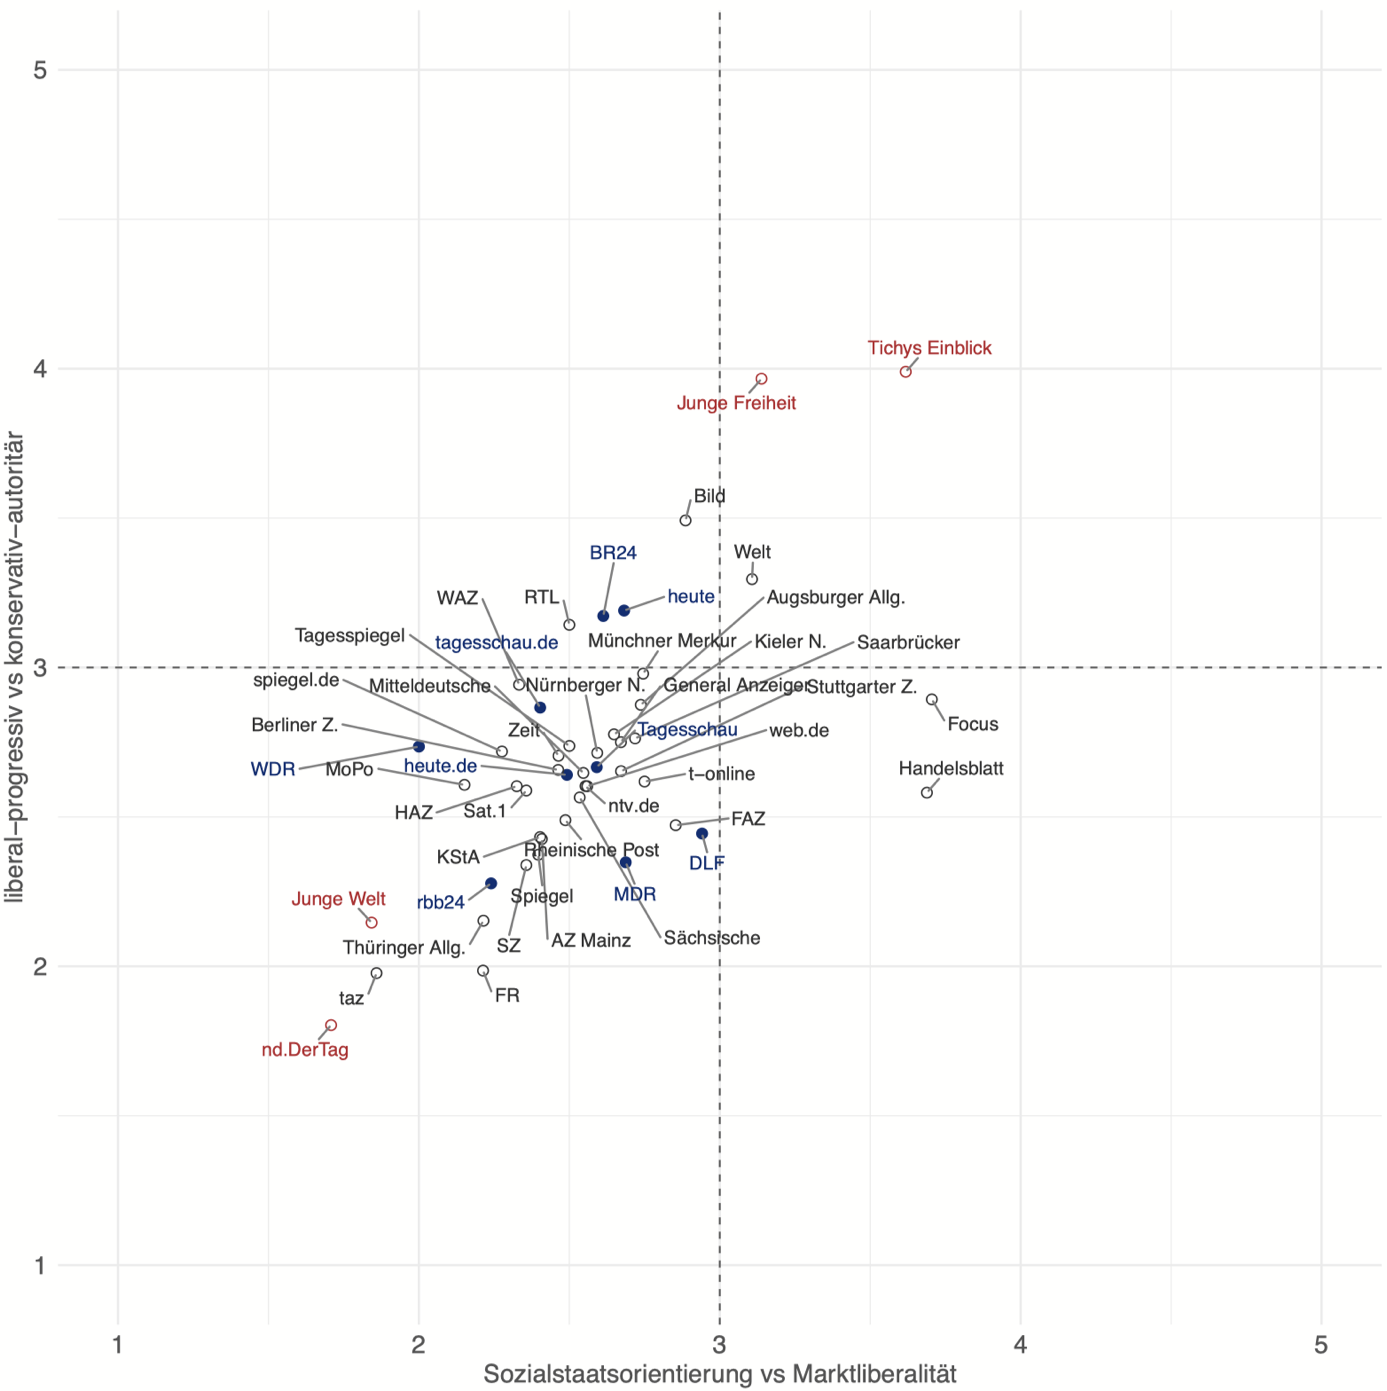
\includegraphics[width=\textwidth]{figures/media/image10.png}
  \caption{\label{fig:medien-ideologie-verortung}Verortung großer deutscher Medien in Hinblick auf ihre „ideologische Grundpositionierung`` (Abbildung 9 aus \citealt[17]{maurerFehltWasPerspektivenvielfalt2024}).}
\end{figure}

Dadurch, dass keine Boulevardmedien wie etwa die \textsc{Bild} oder Online-Medien des rechten Randes wie \textsc{Pi-News} oder \textsc{Compact} in das Korpus aufgenommen wurden, ist zu erwarten, dass die analytische Kontrastierung eher subtile Unterschiede im Framing von Extremismusvarianten zu Tage fördert denn grundlegend verschiedene Konzeptualisierungen. Es wurden also gewissermaßen Steinbrüche für die Erprobung des neu zu entwickelnden Werkzeugs ausgewählt, von denen eine gewisse Gleichartigkeit zu erwarten ist. Die ist auch insofern von Bedeutung, als die diachron geschichteten Subkorpora nicht nach Zeitungen getrennt untersucht werden und insofern eine gewisse Homogenität erfordern. Durch die ebenfalls erfolgende medienkonstrastive Analyse kann im Zeitungsvergleich divergierendes Framing im Anschluss genauer unter die Lupe genommen werden.

Letztlich ist auch zu reflektieren, dass sich mit der Entscheidung für Zeitungstexte auch eine Fortschreibung des „›written language bias‹ (vgl. Linell {[}1982{]} 2005), der in diskurslinguistischen Untersuchungen kritisch reflektiert werden sollte`` \autocite[39]{spitzmullerDiskurslinguistikEinfuhrungTheorien2011}, ergibt. Dies ist nicht von der Hand zu weisen und es wäre wünschenswert, mehr gesprochensprachliche Daten in Untersuchungen einzubeziehen; in der vorliegenden Untersuchung etwa journalistische Funk- und Fernsehbeiträge. Dem stehen jedoch forschungspraktische Gründe entgegen, da automatische Transkriptionsverfahren, die für den Aufbau eines Korpus in repräsentativer Größe notwendig sind, noch keine ausreichend guten Ergebnisse liefern. Es ist des Weiteren sinnvoll, im Rahmen der Entwicklung einer neuen korpuslinguistischen Methode auf vergleichsweise niedrigschwellig zu erlangende und zu prozessierende Daten zurückzugreifen, um sich nicht zu viele Herausforderungen zugleich ‚einzukaufen`.

\subsection{Verwendete Korpus-Software}\label{verwendete-korpus-software}

Die bei der Korpusaufbereitung und -Analyse eingesetzte Software musste in der Lage sein, ein sehr großes Korpus von über einer Milliarde Token verarbeiten zu können. Aus diesem Grund konnte auf verbreitete Tools wie die bezahl- bzw. lizenzpflichtige \emph{Sketch Engine} \autocite{kilgarriffSketchEngineTen2014} oder \emph{\#LancsBox} \autocite{brezinaLancsBoxV5x2020}, das nur vergleichsweise kleine Korpora von unter 10 Millionen Token noch effizient verarbeiten kann,\footnote{Siehe die FAQ unter \url{http://corpora.lancs.ac.uk/lancsbox/docs/pdf/FAQ.pdf}, S. 5. {[}18.12.2025{]}. Die neue Version \emph{\#LancsBox X} \autocite{brezinaLancsBox2023} ist auch in der Lage, größere Korpora zu händeln.} nicht zurückgegriffen werden. Es wurde daher entschieden, mit der \emph{Corpus Workbench} \autocite[CWB,][]{evertTwentyfirstCenturyCorpus2011} zu arbeiten, die in der Lage ist, große Korpora zu prozessieren und auf unterschiedlichen Annotationsebenen durchsuchbar bzw. analysierbar zu machen. Auch Kollokationsanalysen können flexibel auf unterschiedlichen Annotationen durchgeführt werden, was nicht in jedem Korpus-Tool möglich ist, in der hier entwickelten Methode jedoch genutzt wurde. Die Aufbereitung des Korpus folgte in Hinblick auf den Import in die CWB weitenteils Bubenhofers Einführung in die Korpuslinguistik \autocite*{bubenhoferEinfuhrungKorpuslinguistikPraktische2006}; weitere Schritte der Datenaufbereitung werden ausführlicher in den Kapiteln \ref{kenndaten-zum-korpus-und-korpusaufbereitung} und \ref{technisch-methodische-umsetzung-vom-rohen-text-zum-graphen} dargestellt.

Zur flexiblen Durchsuchung der CWB wurde mit dem \emph{R}-Package \emph{polmineR} \autocite{blaettePolmineRVerbsNouns2020} gearbeitet, das es ermöglicht, in der Programmiersprache \emph{R} mit der CWB zu kommunizieren. Es können so Abfragen gemacht werden, deren Ergebnisse unmittelbar im Anschluss in Visualisierungen überführt oder weiteren korpuslinguistischen Analysen unterzogen werden können. Es wurden mithilfe von \emph{polmineR} bzw. der CWB die Kollokations- und Keyword-Analysen sowie einzelne Konkordanz-Suchen durchgeführt.

Die Berechnung, das Clustering und die Exploration von Word Embeddings wurde in der Programmiersprache \emph{Python} und mithilfe des \emph{Word2Vec}-Moduls der \emph{Gensim}-Bibliothek \autocite{rehurekSoftwareFrameworkTopic2010} bzw. dessen Erweiterung \emph{Temporal Word Embeddings with a Compass} \autocite[TWEC,][]{dicarloTrainingTemporalWord2019} vorgenommen. Die Aufbereitung der Kollokations- und Word-Embedding-Daten als Netzwerkgraph geschah mit \emph{visNetwork}\footnote{\url{https://github.com/datastorm-open/visNetwork} {[}18.12.2025{]}}, der \emph{R}-Implementation des \emph{vis-network} Moduls der \emph{vis.js}-Bibliothek\footnote{\url{https://github.com/visjs/vis-network} {[}18.12.2025{]}}.

\subsection{Kenndaten zum Korpus und Korpusaufbereitung}\label{kenndaten-zum-korpus-und-korpusaufbereitung}
\largerpage
Im Rahmen der Datenerhebung wurden alle online ohne Zugangsbeschränkung verfügbaren Artikel der Online-Portale der Zeitungen bis einschließlich August 2021 gesammelt. Insgesamt wurden so 5\,207\,231 Texte bzw. rund 2 Mrd. Token erhoben, die sich in ungleichen Anteilen auf die drei Zeitungen verteilen (19,37 \% \textsc{Taz}, 18,40 \% \textsc{Spiegel}, 62,22 \% \textsc{Welt}). An Metadaten wurden neben publizierender Zeitung und Publikationsdatum auch Ressort, Autor*in, redaktionell vergebene Keywords und die URL erhoben. Im weiteren Verfahren werden davon jedoch nur das Publikationsdatum sowie die veröffentlichende Zeitung genutzt. In einem ersten Versuch konnte das Korpus aufgrund seiner Größe nicht in die CWB eingepflegt werden. Es wurde daher entschieden, ein Sampling der übermäßig repräsentierten \textsc{Welt}-Texte vorzunehmen und diese auf den Umfang der anderen Zeitungen zu reduzieren. Zu diesem Zweck wurden, diachron gleichmäßig verteilt, ca. 35 Prozent der \textsc{Welt}-Texte pro Monat zufällig aus dem Korpus entfernt, sodass das Korpus insgesamt (nicht jedoch in jedem Zeitabschnitt) medial ausgewogen ist (siehe~\figref{fig:subkorpora-umfang}). Es ergibt sich so ein 1\,282\,346\,988 Token umfassendes Korpus\footnote{Dieser und die nachfolgend genannten Token-Werte wurden in \emph{polmineR} mit der Funktion \emph{size()} ermittelt.}, das in acht diachrone sowie drei zeitungsspezifische Subkorpora untergliedert wurde.

Marchi geht ausführlich auf Fragen der diachronen Korpusgliederung ein und unterscheidet drei Varianten:

\begin{quote}
We can consider three ways to determine the level of aggregation of consecutive time periods in order to identify time units:

1 Text-lifecycle segmentation: based on the periodicity characterising the text type (e.g. a daily edition for a newspaper).

2 Top-down segmentation: based on standardised spans (typically a calendar year), or on contextual historical knowledge (e.g. a timeline of events), which is used to inform the segmentation (see for example Bartley \& Hidalgo-Tenorio 2016).

3 Bottom-up segmentation: based on internal variability, i.e. using distributional information to identify milestones in time, which can in turn be used to divide the corpus in subsets of data to compare against one another (Gries 2011).

I would like to argue that no one of these solutions is intrinsically optimal, but that the value of appropriateness always depends on the research questions. \autocite[179-180]{marchiDividingDataEpistemological2018}
\end{quote}

Die zeitliche Einteilung in dieser Arbeit entspricht Variante 2 und die diachronen Subkorpora umfassen jeweils drei Jahre. Eine Ausnahme ist das Subkorpus 2020--2021, das nur Daten bis einschließlich August 2021 umfasst. Dabei wurden also keine diskursspezifisch-inhaltlichen Kriterien wie einschneidende Gewaltereignisse bei Czulo et al. \autocite*{czuloEinflussExtremistischerGewaltereignisse2020} herangezogen, sondern kalendarische Einheiten. Diese sind in Bezug auf den Inhalt agnostisch und insofern zur datengeleiteten Ermittlung des Framings von Extremismus geeigneter, bei dem gewisse Ereignisse bzw. Handlungen extremistischer Akteure ja erst im Rahmen der Analyse aufgedeckt werden sollen. Möglichkeiten einer \emph{bottom-up segmentation} mithilfe strukturentdeckender Verfahren zu prüfen, wäre ein interessantes Desiderat, konnte aber im Rahmen dieser Arbeit nicht realisiert werden.

Der Umfang der Subkorpora wird in~\figref{fig:subkorpora-umfang} dargestellt; Tabelle 1 im Anhang umfasst die genauen Werte sowie die anteilige Verteilung der Zeitungen auf die diachronen Teilkorpora und \emph{vice versa}.

\begin{figure}
  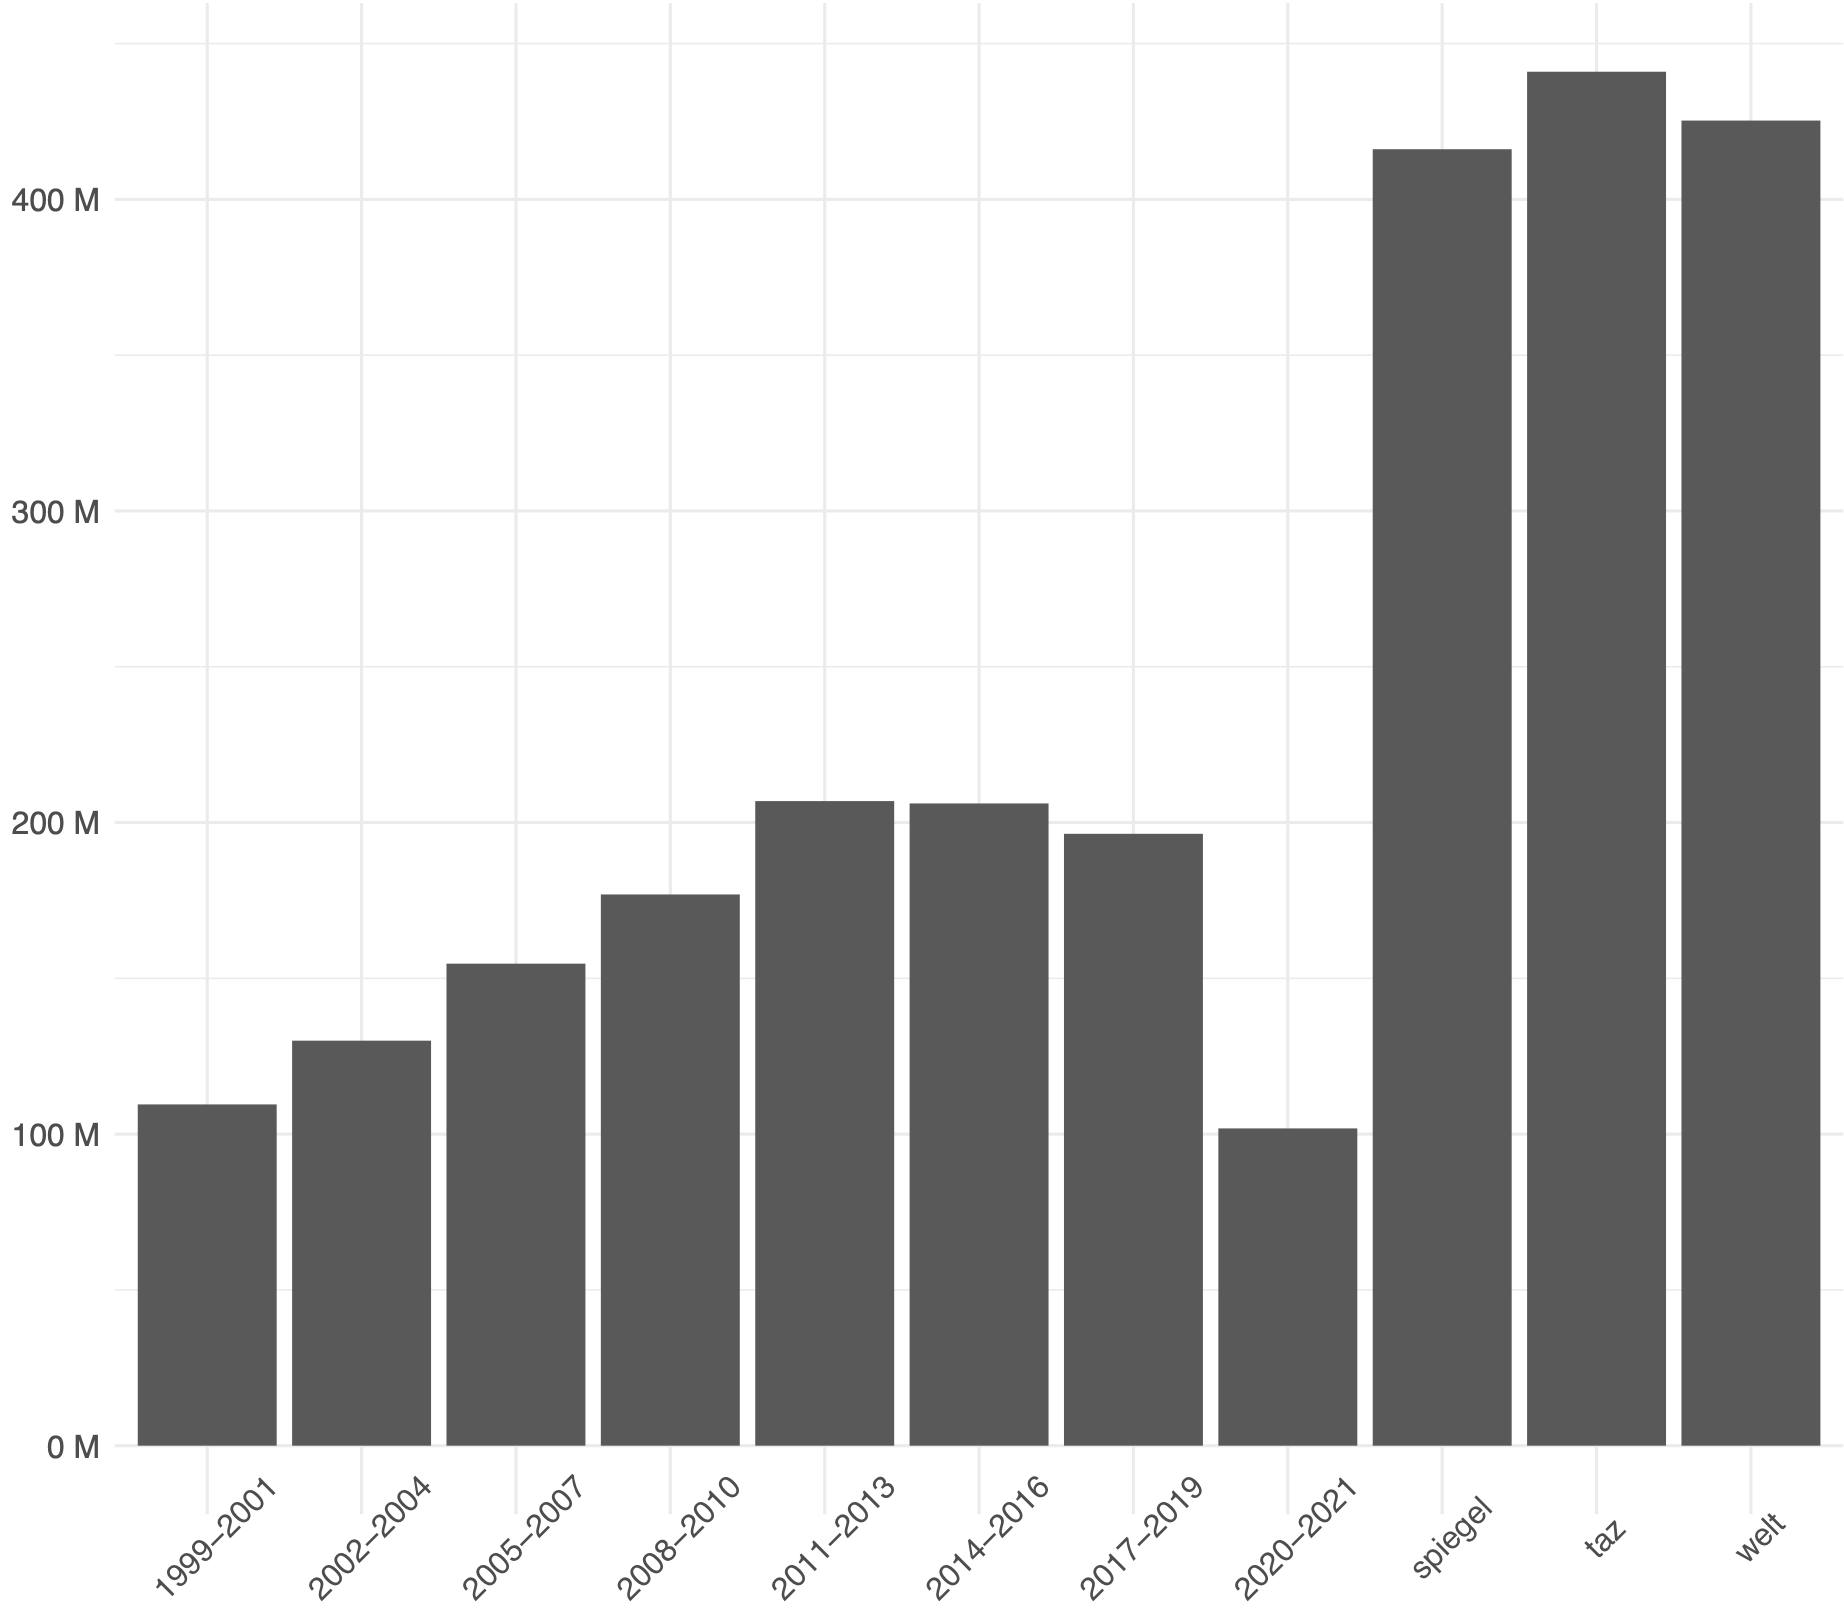
\includegraphics[width=\textwidth]{figures/media/image11.png}
  \caption{\label{fig:subkorpora-umfang}Umfang der Subkorpora in Millionen Token.}
\end{figure}


Die hier zugrundeliegende Tokenisierung wurde mit dem \emph{TreeTagger} \autocite{schmidProbabilisticPartSpeechTagging1994} vorgenommen, der zugleich ein POS-Tagging sowie eine Lemmatisierung des Korpus durchführte. Letztere Annotationen wurden im weiteren Verlauf jedoch kaum genutzt; einerseits um mögliche Fehlerquellen zu vermeiden, andererseits um das Bedeutungspotenzial der sprachlichen Oberfläche auszuschöpfen. Dass einzelne Wortformen einen deutlichen semantischen Mehrwert im Vergleich zur Arbeit mit Lemmata bieten, haben bereits Sinclair und Tognini-Bonelli herausgestellt (siehe \chapref{der-corpus-driven-ansatz}). Und auch Bubenhofer \autocite*[124-129]{bubenhoferSprachgebrauchsmusterKorpuslinguistikAls2009} weist auf das paradoxe Verhältnis hin, dass die Nutzung zusätzlicher Annotationen (auch) einen „Informationsverlust`` bedeutet. So zeigt sich auch im vorliegenden Korpus, dass z.\,B. im Zeitraum 2011--2013 das (ein Wort umfassende) Cluster \cluster{11\_Personen} eng mit dem thematischen Bereich ‚Straftaten \& Juristisches` assoziiert ist (u.\,a. \cluster{11\_Verdächtigen{\breakbar}Tatverdächtigen{\breakbar}mutmaßlichen\_Täter}, \cluster{11\_beschuldigt{\breakbar}verdächtigt{\breakbar}angeklagt}, \cluster{11\_Durchsuchungen{\breakbar}Razzia{\breakbar}Razzien}), während \cluster{11\_Person} im Singular ein deutlich anderes Kollokationsprofil aufweist und mit Clustern wie \cluster{11\_Verhalten}, \cluster{11\_Papst\_Franziskus{\breakbar}Franziskus{\breakbar}Vatikan}, \cluster{11\_Fragen} und \cluster{11\_Identität{\breakbar}Herkunft} vorkommt. Ein weiterer essenzieller Schritt bei der Korpusaufbereitung bestand darin -- Bubenhofer \autocite*{bubenhoferExplorationSemantischerRaeume2022} folgend --, signifikante, unmittelbar aufeinander folgende Wortverbindungen zu identifizieren und zu je einem Token zusammenzuführen. Dazu wurde die \emph{Phrases}-Funktion der \emph{Gensim}-\emph{Python}-Bibliothek eingesetzt (siehe auch \chapref{details-der-korpusaufbereitung}). Es wurden so zunächst signifikante Bi-Gramme identifiziert und -- markiert durch einen Unterstrich -- in das Korpus übernommen (z.\,B. \emph{Angela\_Merkel}). Der Vorgang wurde daraufhin wiederholt, um auch signifikante Tri-Gramme zu identifizieren. In seltenen Fällen, nämlich wenn zwei Bi-Gramme signifikant häufig aufeinander folgen, ergaben sich so auch 4-Gramme wie \emph{mutmaßlich\_rassistisch\_motivierten\_Anschlag}. Dieser Aufbereitungsschritt bildet nicht nur ab, dass sich Bedeutungseinheiten keinesfalls entlang von (orthographischen) Wortgrenzen ziehen lassen und approximiert so \emph{extended units of meaning} im Sinne Sinclairs \autocite*{sinclairUnitsMeaning1996}. Er leistet auch für Type-basierte Verfahren wie Kollokationen und Word Embeddings einen wichtigen Beitrag zur Disambiguierung. So wäre es in Bezug auf die Jugendorganisation der AfD wenig sinnvoll, Kollokationen oder benachbarte Embeddings zu \emph{Junge} oder \emph{Alternative} zu betrachten, da diese über alle Vorkommen der Ausdrücke berechnet werden. \tabref{tab:phrasing} zeigt die jeweiligen paradigmatischen Nachbarn der Ausdrücke und macht den Vorteil des Phrasings deutlich.\footnote{Die Tokenanzahl in den so prozessierten Korpora liegt etwa 20 \% unter den oben berichteten Werten, die genauen Werte finden sich in Tabelle 2 im Anhang.} Letztlich ist dieser Schritt auch unter Frame-semantischer Perspektive vorteilhaft, da auch \emph{FrameNet} Mehrworteinheiten als LE berücksichtigt \autocite[10]{ruppenhoferFrameNetIIExtended2016}.


\begin{table}
  \caption{Nächste Nachbarn im Word-Embedding-Modell 2020--2021 zu \emph{Junge}, \emph{Alternative} und \emph{Junge\_Alternative} mit Cosinus-Ähnlichkeit.}
  \label{tab:phrasing}
   \begin{tabularx}{\textwidth}{llX}
    \lsptoprule
              \emph{Junge}                    & \emph{Alternative}             & \emph{Junge\_Alternative} \\ % Header row
    \midrule
    \emph{junger\_Mann} (0.71)      & \emph{Ergänzung} (0.67)        & \emph{jA} (0.88)          \\
    \emph{Mann} (0.66)              & \emph{Alternativen} (0.66)     & \emph{Verfassungsschutz\_stuft} (0.80) \\
    \emph{Hund} (0.66)              & \emph{Option} (0.65)           & \emph{AfD-Flügel} (0.77)  \\
    \emph{Kleinkind} (0.65)         & \emph{echte\_Alternative} (0.62) & \emph{Nachwuchsorganisation} (0.75) \\
    \emph{Bub} (0.65)               & \emph{bessere\_Alternative} (0.56) & \emph{Beobachtungsfall} (0.73) \\
    \emph{elfjährige} (0.64)        & \emph{Lösung} (0.55)           & \emph{Gesamtpartei} (0.72) \\
    \emph{Säugling} (0.64)          & \emph{Blaupause} (0.54)        & \emph{rechtsextrem} (0.71) \\
    \emph{Teenager} (0.64)          & \emph{sinnvolle\_Ergänzung} (0.52) & \emph{rechtsextremen\_Verdachtsfall} (0.70) \\
    \emph{Baby} (0.63)              & \emph{Parallele} (0.52)        & \emph{Beobachtungsobjekt} (0.68) \\
    \emph{Senior} (0.63)            & \emph{Möglichkeit} (0.52)      & \emph{Identitäre\_Bewegung} (0.68) \\
    \lspbottomrule
   \end{tabularx}
  \end{table}

\tabref{tab:type_frequencies} weist die Type-Mengen pro Subkorpus aus und berichtet darüber hinaus, wie viele Types mindestens 25-mal im Korpus vorkommen und mithin bei der Berechnung der Word-Embedding-Modelle einbezogen wurden (siehe \chapref{berechnung-und-clustering-der-word-embedding-modelle}). Da durch die Mindestfrequenz ein großer Teil des \emph{long tail} der Zipfschen Häufigkeitsverteilung von Wörtern abgeschnitten wird, machen sie nur einen Bruchteil der gesamten Type-Menge aus.

\begin{table}
  \caption{Type-Anzahlen und Type-Anzahlen mit einer Mindestfrequenz von 25 pro Subkorpus.}
  \label{tab:type_frequencies}
   \begin{tabular}{lrr}
    \lsptoprule
    Subkorpus     & Types      & Types $\geq$ 25\\ %table header
    \midrule
    1999--2001  & 2541673  & 132041 \\
    2002--2004  & 2759025  & 148597 \\
    2005--2007  & 2994777  & 168204 \\
    2008--2010  & 3048237  & 183405 \\
    2011--2013  & 3196110  & 203417 \\
    2014--2016  & 3163474  & 201286 \\
    2017--2019  & 2910547  & 190915 \\
    2020--2021  & 1864503  & 110389 \\
    \textsc{Taz}  & 5789089  & 365815 \\
    \textsc{Spiegel} & 4883715  & 342740 \\
    \textsc{Welt} & 5002421  & 355619 \\
    \lspbottomrule
   \end{tabular}
  \end{table}

\section{Methodik und Operationalisierung}\label{methodik-und-operationalisierung}

\subsection{Prozess der Methodenentwicklung}\label{prozess-der-methodenentwicklung}

Dieses Kapitel soll einen kurzen Überblick über das Vorgehen bei der Entwicklung der Methode geben sowie ihre Funktionsweise in Kürze skizzieren. In den folgenden Abschnitten wird anschließend ausführlicher auf methodische Hintergründe, Operationalisierungen und die technische Realisierung eingegangen. Das Ansinnen war es, semantische Frames im Sinne Busses \autocite*{busseFrameSemantikKompendium2012} in einem datengeleiteten Zugriff kontextspezifisch zu rekonstruieren. Dabei sollte geprüft werden, inwiefern dies in einem quantitativen, datengeleiteten Zugriff möglich ist: Zum einen sollte die Bearbeitung großer und repräsentativer Korpora ermöglicht werden, zum anderen über einen distributionell-semantischen Zugriff die Bedeutung sprachlicher Einheiten erfasst und zu den ermittelten Frames bzw. Frame-Strukturen in Beziehung gesetzt werden. Die Hypothese ist dabei, dass (Frame\mbox{-})semantische Strukturen distributionellen Strukturen der sprachlichen Oberfläche entsprechen und dass beide in einem emergentistischen Zugang freigelegt werden können. Ein besonderes Potenzial der Nutzung quantitativer Verfahren liegt auch in der Ermöglichung einer probabilistischen Modellierung, die Frame-Relationen gegenstandsadäquat nicht absolut, sondern als graduelles Phänomen beschreiben kann.

Die Methode wurde in einem explorativen Prozess entwickelt, in dem mit unterschiedlichen korpuslinguistischen Verfahren experimentiert wurde, die sich in Diskursanalysen bewährt haben (siehe \chapref{distributionell-semantische-methodik}). Recht bald bewies sich das Potenzial von Word Embeddings, Wortsemantik zu erfassen und in einem quantitativen Zugang untersuchbar zu machen. Auch dass die paradigmatische Distribution der Wörter im Vektorraum als FE interpretierbar ist, wurde deutlich und durch eine Cluster-Analyse systematisch umgesetzt (siehe \chapref{geclusterte-word-embeddings-als-frame-elemente}). Frame-Relationen zwischen den FE wiederum konnten anschließend über das etablierte Verfahren der Kollokationsanalyse abgebildet werden. In \emph{corpus-driven} Manier wurden dabei die Kollokationen aller FE miteinander berechnet, was die Analyse und Visualisierung als rekursive Netzwerkstruktur, d.\,h. als Kollokationsnetzwerk, und mithin die Realisierung Frame-theoretischer Annahmen zur Organisation von Frames, ermöglichte (\chapref{kollokation-von-word-embedding-clustern-als-frame-relationen-und-perspektivierung-kollokationsnetzwerke-als-frames}--\ref{netzwerk-communities-als-thematische-teil-frames}). Nach weiteren methodischen Schritten der quantitativen Informationsanreicherung können die so korpus- bzw. kontextspezifisch ermittelten Frames dann interpretiert und kontrastiert werden. Leitlinien bei der Methodenentwicklung waren, dass die ermittelten diskursiven Frame-Strukturen sowohl in Hinblick auf Frame-semantische Annahmen als auch auf die kondensierten minimalen Anforderungen an einen Extremismus-Frame (\chapref{inhaltliche-mindestanforderungen-an-einen-extremismus-frame}) fruchtbar zu interpretieren sein mussten.

Die entwickelte Methode wurde unter dem Namen \emph{FDgrapher} (\emph{Frame and Discourse Grapher}) auf GitHub (\url{https://github.com/feldmueller/FDgrapher}) veröffentlicht.

\subsection{\texorpdfstring{Begriffsklärungen: Quantitativ und qualitativ -- \emph{corpus-driven} und \emph{corpus-based} sowie die Rolle von Hermeneutik}{Begriffsklärungen: Quantitativ und qualitativ -- corpus-driven und corpus-based sowie die Rolle von Hermeneutik}}\label{begriffsklaerungen-quantitativ-und-qualitativ-corpus-driven-und-corpus-based-sowie-die-rolle-von-hermeneutik}

\chapref{der-corpus-driven-ansatz} hat die grundlegenden Herangehensweisen von \emph{corpus-driven} und \emph{corpus-based} Ansätzen bereits skizziert. Im Folgenden sollen die Begriffe noch einmal präziser gefasst und in Hinblick auf konkrete Methoden sowie die Begriffe ‚quantitativ` und ‚qualitativ` (im Kontext korpuslinguistischer Arbeiten) verortet werden. Dies erscheint mir notwendig, da es seit der Prägung der Begriffe einerseits methodische Neuerungen, andererseits auch einen semantischen Wandel der Termini gegeben hat. Die Analyse einzelner Konkordanzen etwa, wie Tognini-Bonelli \autocite*{tognini-bonelliCorpusLinguisticsWork2001} sie zum zentralen Bestandteil ihrer Analysen macht, würdeheute wohl nicht mehr als \emph{corpus-driven} bezeichnet werden.

Die im Folgenden vorgenommene definitorische Unterteilung orientiert sich an Meißner et al. \autocite*{meissnerKorpusanalyse2016}, die korpuslinguistische Methoden einerseits in quantitative und qualitative, andererseits in korpus- und einheitenbezogene Verfahren unterteilen. Als ‚quantitative` Verfahren fasse ich mit Meißner et al. \autocite*[309]{meissnerKorpusanalyse2016} alle Korpusmethoden, die primär auf dem systematischen „Zählen von Einheiten`` beruhen und dabei sowohl Token bzw. Types als auch beliebige andere Korpusannotationen zur Grundlage der Zählung machen können. Im Gegensatz dazu begreife ich als ‚qualitativ` solche Methoden, die primär auf die Lektüre einzelner Belegstellen oder ganzer Texte zurückgreifen.

Zusätzliche Definitionselemente stellen m.\,E. eine unnötige Verengung der Begriffe dar. So heißt es bei Meißner et al. weiter zur quantitativen Methodik:

\begin{quote}
Ein Vorgehen im Sinne einer quantitativen Korpusanalyse bedeutet, den Untersuchungsgegenstand in suchbarer und auszählbarer Form zu operationalisieren und dabei theoretische Konzepte in empirische Häufigkeiten zu übersetzen. Die Fragestellung wird dabei so formuliert, dass die Häufigkeit, welche im Korpus unter den in Frage stehenden Bedingungen ermittelt wird, die abhängige Variable darstellt (vgl. Stefanowitsch 2005). \autocite[309]{meissnerKorpusanalyse2016}
\end{quote}

Dieses Vorgehen ist in der Praxis zwar in der Tat häufig anzutreffen und entspricht der klassischen quantitativen hypothesentestenden Methodik. Die Definition lässt jedoch \emph{corpus-driven} verfahrende Ansätze außer Acht, die gerade nicht mit vorausgesetzten theoretischen Konzepten und deren Operationalisierung arbeiten, sondern aus frequenzbasierten Daten theoretische Konzepte ableiten. Auch „das Ziel bestimmte in den Korpusdaten abgebildete (sprachliche) Phänomene zunächst zu ermitteln, sie zu klassifizieren, einzuordnen und zu interpretieren``, wie Meißner et al. \autocite*[312]{meissnerKorpusanalyse2016} im Anschluss an Scherer \autocite*{schererKorpuslinguistik2006} als Charakteristikum qualitativer Methoden ansetzen, gilt nur, wenn man quantitativ-datengeleitete Ansätze ignoriert, die ja ebenso verfahren. Letztlich ist gerade die Annahme, dass Interpretation bzw. ein „hermeneutisches Vorgehen`` \autocite[313]{meissnerKorpusanalyse2016} qualitative von quantitativen Ansätzen abgrenzt m.\,E. nicht sinnvoll, wenn auch weit verbreitet.\footnote{So etwa bei Busse \autocite*[202]{busse33LexikFrameanalytisch2017}, der eine „{[}q{]}uantitative oder qualitative (‚objektivistische` oder ‚hermeneutische`) Form der Analyse`` unterscheidet, bei Römer \& Wengeler \autocite*{roemerBackRootsVerteidigungsrede2022} oder aus quantitativer Perspektive bei Ziem \autocite*{ziem3WortschatzII2017}. Siehe aber kritisch z.\,B. Storjohann \& Schröter \autocite*[190-191]{storjohannPrasenzUndAbsenz2013}.} Digitale, quantitative Methoden stellen eine Möglichkeit dar, sprachliche Zeichen durch Transformationen auf neue Art lesbar zu machen \autocite{bubenhoferDigitaleKulturlinguistikDigitalitaet2022}. Sie werden dabei ihrem ursprünglichen Verwendungszusammenhang enthoben und somit -- wie Bubenhofer \autocite*{bubenhoferVisuelleLinguistikZur2020} herausarbeitet -- dekontextualisiert und desequenzialisiert, was zunächst einen Verlust an Informationen bedeutet. Zugleich werden sie jedoch zu anderen -- unter Umständen über das gesamte Korpus verteilten -- Zeichen in Bezug gesetzt und so rekontextualisiert. Eine Keyword-in-Context-Liste (KWiC-Liste) etwa ist

\begin{quote}
eine Anleitung zur Interpretation, die entweder jedem einzelnen Eintrag der Liste gerecht werden will oder aber eine Musterhaftigkeit in ihrem Ensemble sieht. Damit ist die Liste eben nicht nur einfach ein Verweisindex auf die ursprünglichen Kontexte, sondern bildet zusätzlich einen neuen Kontext. \autocite[195]{bubenhoferVisuelleLinguistikZur2020}
\end{quote}

Neben diesem -- gerade für die Diskurslinguistik zentralen -- Potenzial\footnote{Zentral für die Diskursanalyse ist dieses Potenzial besonders dann, wenn Diskursanalyse mit Spitzmüller \& Warnke \autocite*{spitzmullerDiskurslinguistikEinfuhrungTheorien2011} als ‚transtextuelle` Analyse begriffen wird oder mit Busse \autocite*[24]{busseDiskursSpracheGesellschaftliches2013} „als eine Form der Wort-, Satz- oder Textsemantik {[}\ldots{]}, die Beziehungen zwischen Wort- oder Satzbedeutungen und Texten auch dann analysiert, wenn die Bezugsgrößen aus verschiedenen Texten stammen sollten``.} liegt der Wert quantitativ-korpuslinguistischer Verfahren auch darin, Gütekrieterien wie Validität und Reliabilität gerecht zu werden \autocite{scharlothWuchernRhizomeLinguistische2013}. Dies bedeutet jedoch nicht, dass Analyseergebnisse ‚objektiv` wären oder für sich selbst sprechen könnten. Stattdessen müssen sie in einem Zugang, den man mit Schröter \autocite*[363-364]{schroeterWennMenschenAuseinandergehn2012} als ‚quantitative Hermeneutik`\footnote{Ihr Vorgehen ist allerdings primär qualitativ ausgerichtet und die quantitativen Analysen haben nur ergänzenden Charakter, sodass es sich durchaus um eine Neuausrichtung des Begriffs handeln würde.} bezeichnen könnte, gelesen werden. Dabei ist klar, dass der Zugang nicht voraussetzungsfrei ist. Gerade der häufig erhobene Einwand, dass ja das Korpus und seine Zusammenstellung durch die Forschungsperson einen gewichtigen Einfluss auf die Analyseergebnisse habe, trifft natürlich vollkommen zu. Er ist jedoch insofern auch etwas eigentümlich, als es in korpuspragmatischen Analysen ja geradezu darum geht, den Einfluss des Kontextes, den man im Korpusaufbau modellieren möchte, abzubilden; also gerade nicht „die Sprache`` abzubilden, sondern „auf der Basis verschiedener Datensätze unterschiedliche semantische Räume zu modellieren und miteinander zu vergleichen`` \autocite[218]{knuchelMachineLearningUnd2023}. Auch die Wahl der eingesetzten Algorithmen hat einen fundamentalen Einfluss auf die Analyseergebnisse. ‚Objektiv` -- oder vielleicht eher ‚unvoreingenommen` -- sind diese jedoch insofern, als sie „konsequent anti-intentionalistisch{[}{]}`` \autocite[724]{wilkSturmNieWar2021} sind. Sie fördern zwar, gesteuert durch die Forschungsperson, eine bestimmte Musterhaftigkeit zu Tage, etwa in Bezug auf Wortdistributionen. Über diskursive Inhalte wissen sie jedoch nichts. Wenn also durch die Wahl solcher inhaltlich agnostischer Algorithmen Wort-Cluster wie \cluster{14\_Fremdenfeindlichkeit{\breakbar}Intoleranz{\breakbar}Antisemitismus} emergent werden, ist das ein überdeutlicher Hinweis darauf, dass Charakteristika des (Rechts\mbox{-})Extremismus als solche diskursiv realisiert werden, eine Rolle im Framing von Extremismus spielen und für die Frame-Semantik als lexikalische Evokationsmuster einzubeziehen sind. Zusammenzufassen ist also, dass „quantitativ{[}e{]} Analysen {[}\ldots{]} nicht Antworten auf Fragestellungen {[}sind{]}, sondern neue Daten, die vor einem geistes- und sozialwissenschaftlichen Hintergrund genauso hermeneutisch gedeutet werden müssen wie einzelne Texte`` \autocite[25]{bubenhoferWennLinguistikKorpuslinguistik2018}.

Die hier vorgenommene und vergleichsweise einfache Unterteilung ermöglicht es, alle wichtigen korpuslinguistischen Methoden trennscharf zu verorten. Zu den ‚quantitativen` Verfahren zählen so die folgenden von Meißner et al. \autocite*{meissnerKorpusanalyse2016} zusammengetragenen Methoden: die Berechnung und Analyse von Wort- bzw. Frequenzlisten, Keywords, N-Grammen, Kennwerten wie der Type-Token-Ratio, die quantitative Konkordanzsuche\footnote{Bei quantitativen Konkordanzsuchen geht es, anders als in ihrem qualitativen Pendant, nicht um die Lektüre einzelner Belegstellen, sondern um die Ermittlung der Frequenz eines Suchmusters im Korpus.} sowie die Kollokations- und die Kollostruktionsanalyse \autocite{stefanowitschCollostructionsInvestigatingInteraction2003}. Zu ergänzen sind Methoden bzw. Sprachmodelle, die auf komplexen statistischen Verfahren bzw. dem Training neuronaler Netze beruhen wie etwa Word Embeddings, Topic Modelling, Transformer-Sprachmodelle wie BERT \autocite{devlinBERTPretrainingDeep2019} und auch Large Language Models (LLMs) der neuesten Generation wie ChatGPT \autocite{openaiGPT4TechnicalReport2023}. Zu den ‚qualitativen` Verfahren zähle ich lediglich die eingehende Lektüre von Konkordanzen oder ganzer Korpustexte.

Die Unterteilung in \emph{corpus-based} und \emph{corpus-driven} Verfahren weist Überlappungen mit der quantitativ-qualitativ-Abgrenzung auf, ist jedoch von dieser zu unterscheiden. So unterliegt zwar allen \emph{corpus-driven} Korpusmethoden zugleich eine quantitative Funktionsweise und zumindest die qualitative Lektüre einzelner Konkordanzen ist immer \emph{corpus-based}, jedoch können \emph{corpus-based} Methoden sowohl qualitativer als auch quantitativer Natur sein. Im Verständnis dieser Arbeit entspricht die Differenzierung in \emph{corpus-based} und \emph{corpus-driven} Ansätze grob der Unterteilung von Meißner et al. in korpus- und einheitenbezogene Verfahren. Als \emph{corpus-based} bzw. einheitenbezogen verstehe ich alle Methoden, die zu einem vorgegebenen Suchmuster Ergebnisse liefern. Darunter fällt prototypisch die Konkordanzsuche, die in einem qualitativen Zugang genutzt werden kann, um Kotexte des Suchmusters in der KWIC-Ansicht zu betrachten oder auch die „Quantitative Konkordanzsuche`` \autocite[311]{meissnerKorpusanalyse2016}, die nicht auf die Sichtung einzelner Belegstellen, sondern auf die Ermittlung der Frequenz des abgefragten Suchmusters zielt. Als weiteres wichtiges Verfahren fällt die klassische Kollokationsanalyse, die zu einem Suchmuster Kollokate ermittelt, in diese Kategorie. Bei \emph{corpus-driven} bzw. korpusbezogenen Methoden wird hingegen darauf verzichtet, Suchausdrücke zu formulieren. Stattdessen wird das gewählte Verfahren auf das gesamte Korpus und alle auf der anvisierten Korpusebene enthaltenen sprachlichen Einheiten angewandt. So wird etwa bei einer Keyword-Analyse nicht ein einzelnes Wort vorgegeben und daraufhin ermittelt, ob dieses im Korpus signifikant häufiger als in einem Referenzkorpus vorkommt. Stattdessen werden \emph{alle} im Korpus enthaltenen Wörter zu Tage gefördert, die überzufällig häufig im Vergleich zu einem Referenzkorpus vorkommen. Ebenfalls zu den etablierten \emph{corpus-driven} Methoden zählen Wortlisten, N-Gramme, Kennwerte wie die Type-Token-Ratio, Word Embeddings, Topic Modelling, aber auch die Berechnung ganzer Kollokationsnetze, bei denen für jede sprachliche Einheit ein Kollokationswert in Bezug auf jede andere sprachliche Einheit ermittelt wird (so auch im Rahmen dieser Arbeit realisiert). Word Embeddings wiederum können auch in \emph{corpus-based} Manier genutzt werden, wenn nur zu ausgesuchten Wörtern distributionelle Eigenschaften abgefragt werden.

Letztlich ist festzuhalten, dass mithilfe dieser Definitionen zwar eine trennscharfe Zuordnung von Methoden möglich ist, in der Forschungspraxis jedoch quantitative und qualitative Verfahren zumeist kombiniert werden. Insbesondere die qualitative Sichtung von Konkordanzen zu quantitativ ermittelten sprachlichen Einheiten kann ein wichtiger Analyseschritt sein, um quantitative Zusammenhänge zu verstehen und insbesondere detailbezogene Analyseergebnisse abzusichern. So stellt Baker fest:

\begin{quote}
we have to make sure that what we \emph{think} is being counted is actually what the computer is counting. A wise corpus linguist always checks concordance data before drawing conclusions. \autocite[44]{bakerAcceptableBiasUsing2012}
\end{quote}

Während dem ersten Teil des Zitats vollumfänglich zuzustimmen ist und ein gutes Verständnis der verwendeten Methoden und ihrer Aussagekraft immer notwendig ist, ist die umfängliche Sichtung von Textbelegen bei frequenten Mustern und großen Korpora kaum noch möglich. Sie ist aufgrund der (re)kontextualisierenden Eigenschaft korpuslinguistischer Analyseergebnisse aber auch gar nicht immer notwendig:

\begin{quote}
So stehen beispielsweise maschinell berechnete Mehrworteinheiten, die statistisch für bestimmte Akteure, Institutionen oder Zeitepochen typisch sind, im Vordergrund, die anschließend diskurslinguistisch gedeutet werden. Diese Menge an Mehrworteinheiten mit gemeinsamer Typik hinsichtlich eines bestimmten Aspektes sind eine rekontextualisierte Liste -- mit Sprengkraft. Denn -- so die Kritik -- wie sollen die einzelnen Mehrworteinheiten ohne Rückgriff auf die „ursprünglichen`` Kontexte in den „eigentlichen`` Texten korrekt gedeutet werden? Dieser Einwand wird dann zur Konstruktion einer Dichotomie zwischen quantitativen und qualitativen Methoden verwendet und im besten Fall gefordert, dass beides miteinander verbunden werden müsse (Spitzmüller{\slash}Warnke 2011, 39; Niehr 2015, 144). Die Frage ist also, ob die rekontextualisierte Liste ernst genommen wird oder nicht -- ob der Pakt mit dem Teufel eingegangen wird, wie es der Literaturwissenschaftler Franco Moretti ausgedrückt hat: „what we really need is a little pact with the devil: we know how to read texts, now let's learn how not to read them`` (Moretti 2000, 57). \autocites[195]{bubenhoferVisuelleLinguistikZur2020}[siehe auch][]{bubenhoferDreiThesenVisualisierungspraktiken2016}
\end{quote}

Es findet sich des Weiteren eine Reihe methodologischer Vorschläge zur Kombination eher quantitativ-\emph{corpus-driven} ausgerichteter Verfahren mit qualitativ-\emph{corpus-based} Ansätzen. So sprechen etwa Stulpe \& Lemke \autocite*{stulpeBlendedReading2016} von \emph{blended reading} als eine Kombination von \emph{close} und \emph{distant reading} \autocite{morettiConjecturesWorldLiterature2000}; Kalwa \autocite*{kalwaKonstitutionKonzeptenDiskursen2019} spricht von \emph{Zooming in}{\slash}\emph{out} und Bubenhofer \autocite*{bubenhoferQuantitativInformierteQualitative2013} schlägt eine „quantitativ informierte qualitive Diskursanalyse`` vor, bei der qualitativere Analysen auf der Folie quantitativer Ergebnisse vorgenommen werden. In dieser von Bubenhofer vorgeschlagenen Heuristik werden qualitative Untersuchungen vor dem Hintergrund quantitativer Daten vorgenommen. Die Idee ist, dass diskursive Veränderungen und Regelmäßigkeiten besonders gut bei Kenntnis der musterhaften „seriellen Verwendung -- oder gerade auch der seriellen Vermeidung`` \autocite*[130]{bubenhoferQuantitativInformierteQualitative2013} gefunden bzw. aufgezeigt werden können.

\subsection{Methoden der Distributionellen Semantik: Word Embeddings und Kollokationen}\label{methoden-der-distributionellen-semantik-word-embeddings-und-kollokationen}

\subsubsection{Kollokationen als syntagmatische distributionelle Muster}\label{kollokationen-als-syntagmatische-distributionelle-muster}

\subsubsubsection{Was sind Kollokationen?}\label{was-sind-kollokationen}

Die Berechnung von Kollokationen ist eine der wichtigsten Methoden der semantisch interessierten Korpuslinguistik. Begrifflich sind Kollokationen jedoch keinesfalls klar umrissen, Evert \autocite*[15]{evertStatisticsWordCooccurrences2005} spricht von „serious terminological confusion that surrounds the concept of collocations today``. Auf den Punkt bringt es Schmid \autocite*[235]{schmidCollocationHardPin2003}: Kollokationen sind „hard to pin down, but bloody useful``. Während der Begriff bei seinem Schöpfer John Rupert Firth \autocite*[194-195]{firthPapersLinguistics193419511957} noch eine eher vage Bedeutung hatte und das übliche (auch im Sinne des frequenten) gemeinsame Vorkommen von Wörtern bezeichnete (siehe auch \chapref{distributionelle-semantik}), haben sich im Laufe der Zeit in unterschiedlichen Forschungstraditionen verschiedene Definitionen etabliert. Zugrundegelegt werden dabei zum Teil eher frequenzbezogene, sprachstatistische Kriterien, zum Teil auch grammatische Dependenzbeziehungen oder Idiomatizität. Zur terminologischen Differenzierung wird mitunter der Begriff der ‚Kookkurrenz` herangezogen, der jedoch gleichermaßen heterogen verwendet wird. So sind für Bubenhofer Kollokationen durch ihr statistisch signifikant häufiges gemeinsames Auftreten in einem Korpus gekennzeichnet, wohingegen der Begriff der ‚Kookkurrenz` einfach gemeinsames Ko-Vorkommen meint:

\begin{quote}
Unter ‚Kollokationen` verstehe ich statistisch auffällige Kookkurrenzen. Das Plus von Kollokationen gegenüber Kookkurrenzen liegt also nur im statistischen Maß der überzufälligen Kombination. Kookkurrenzen beschreiben demnach in einem Syntagma aufeinander treffende Wörter, von denen nicht weiter bekannt ist, ob ihre Verbindung statistisch signifikant oder überhaupt besonders frequent ist. \autocite[122]{bubenhoferSprachgebrauchsmusterKorpuslinguistikAls2009}
\end{quote}

Auch bei Lemnitzer und Zinsmeister ist der Kollokationsbegriff ein Hyponym des Kookkurrenzbegriffes, sie setzen das Kriterium der statistischen Signifikanz allerdings bereits für Kookkurrenzen an und definieren Kollokationen sodann systemlinguistisch:

\begin{quote}
Eine Kollokation muss natürlich den oben genannten Kriterien {[}zur Kookkurrenz, T.F.{]} genügen, darüber hinaus aber auch eine innere Struktur, in Form einer Hierarchie zwischen Kollokationsbasis und Kollokator aufweisen. Darüber hinaus müssen die Glieder einer Kollokation in einer syntaktischen Beziehung zueinander stehen, z.\,B. als Kopf einer Verbalphrase und Kopf einer gleich- oder untergeordneten Nominalphrase, oder als Kopf einer Nominalphrase und Kopf einer untergeordneten Adjektivphrase. \autocite[179]{lemnitzerKorpuslinguistikEinfuhrung2015}
\end{quote}

Als Beispiele für so definierte Kollokationen geben sie etwa \emph{Zähne putzen}, \emph{Schlange stehen}, \emph{den Tisch decken} und \emph{dichtes Haar} an. Vor dem Hintergrund der vorliegenden umfangreichen (Überblicks\mbox{-})Literatur zu Kollokationen \autocites[siehe etwa][]{storjohannKookkurrenzAusKorpuslinguistischer2016, almela-sanchezLexicalCollocationAnalysis2018, bubenhoferSprachgebrauchsmusterKorpuslinguistikAls2009, evertStatisticsWordCooccurrences2005, stefanowitschCorpusLinguisticsGuide2020} sei an dieser Stelle darauf verzichtet, weitere Begriffsdefinitionen und -ansätze darzustellen. Definitorisch folge ich Bubenhofer und fasse Kollokationen als das überzufällig häufige Ko-Vorkommen von sprachlichen Einheiten auf, das korpuslinguistisch mithilfe unterschiedlicher Maße gemessen werden kann und so auch eine graduelle Auskunft über die Kollokationsstärke gibt. Dass dieser Ansatz „lumps together units that are linguistically quite different`` \autocite[231]{grangerFormulaicSequencesLearner2018}, also unterschiedliche Wortarten und neben Autosemantika auch Synsemantika zu Tage fördert, ist dabei in einer datengeleiteten Diskursanalyse nicht problematisch, sondern hat das Potenzial, auch unauffällige musterhafte Sprechweisen freizulegen.

\subsubsubsection{Wie funktioniert die Berechnung von Kollokationen?}\label{wie-funktioniert-die-berechnung-von-kollokationen}

Grundlage der Berechnung von Kollokationen sind drei wesentliche Parameter: die Suchanfrage, das Kollokationsfenster und das statistische Maß, das über Signifikanz und Rangfolge der Ergebnisse entscheidet. Mit der Suchanfrage wird das sprachliche Muster festgelegt, zu dem Kollokatoren im Korpus ermittelt werden sollen. In der Regel sind dies einzelne Wörter, d.\,h. Wortformen oder Lemmata. Es ist jedoch auch denkbar -- je nach Möglichkeiten der Korpussoftware -- auf beliebigen anderen Annotationsebenen zu suchen. So lässt sich z.\,B. abfragen, welche POS-Tags miteinander vorkommen oder -- wie in der folgenden Analyse -- welche Wort-Cluster Kollokationen bilden. Die Suchanfrage zu den Ergebnissen der Kollokationsanalyse in \tabref{tab:collocation_analysis}, die mit \emph{polmineR} im Teilkorpus 2020--2021 durchgeführt wurde, lautet etwa \emph{cooccurrences(``{[}word = `Hanau'{]}'', l = 5, r = 5, method = ``ll'', cqp = TRUE)}. Sie legt fest, dass Kollokationen zur Wortform \emph{Hanau} berechnet werden sollen, dass das Kollokationsfenster je fünf Wörter zur linken und rechten des Wortes umfassen soll, dass als statistisches Maß die \emph{Log-Likelihood} \autocite{dunningAccurateMethodsStatistics1993} verwendet werden soll sowie als Abfragesprache CQP \autocite{evertTwentyfirstCenturyCorpus2011}. \tabref{tab:collocation_analysis} listet die von \emph{polmineR} bzw. der unterliegenden CWB ausgegebenen Werte. \emph{Count\_coi} zeigt dabei an, dass z.\,B. \emph{Anschlag} 358 Mal im Umfeld von \emph{Hanau} auftaucht; \emph{count\_ref}, dass \emph{Anschlag} 3179 Mal ohne \emph{Hanau} auftritt. Bei einer zufälligen Verteilung der Wörter im Korpus wäre allerdings davon auszugehen, dass \emph{Anschlag} nur 1,42 Mal (\emph{exp\_coi}) mit \emph{Hanau} kookkurriert und 3535,58 Mal ohne \emph{Hanau} (\emph{exp\_ref}). Diese Diskrepanz bedingt sodann den errechneten \emph{Log-Likelihood}-Wert (\emph{ll}) von 3288,71.

\begin{table}
\caption{Beispiel-Output einer Kollokationsanalyse mit \emph{polmineR} zu \emph{Hanau} im Subkorpus 2020--2021.}
\small
\label{tab:collocation_analysis}
 \begin{tabular}{lrrrrr}
  \lsptoprule
  word & count\_coi & count\_ref & exp\_coi & exp\_ref & ll \\
  \midrule
  \emph{Anschlag}              & 358   & 3179    & 1.42   & 3535.58   & 3288.71 \\
  \emph{Halle}                 & 245   & 5235    & 2.20   & 5477.80   & 1837.30 \\
  \emph{in}                    & 1856  & 1749678 & 701.88 & 1750832.12 & 1344.40 \\
  \emph{Opfer}                 & 227   & 11983   & 4.89   & 12205.11  & 1303.45 \\
  \emph{von}                   & 1122  & 837359  & 336    & 838145    & 1153.76 \\
  \emph{rassistischen\_Anschlag} & 78  & 15      & 0.04   & 92.96     & 1138.29 \\
  \emph{nach}                  & 681   & 335175  & 134.59 & 335721.41 & 1125.60 \\
  \emph{neun}                  & 172   & 9137    & 3.73   & 9305.27   & 985.25 \\
  \emph{Hanau}                 & 100   & 3160    & 1.31   & 3258.69   & 673.52 \\
  \emph{Anschlags}             & 60    & 409     & 0.19   & 468.71    & 580.38 \\
  \lspbottomrule
 \end{tabular}
\end{table}

Das Kollokationsfenster als zweiter festzulegender Parameter bestimmt, wie viele Wörter zur Rechten und Linken der jeweiligen Treffer der Suchanfrage als potenzielle Kollokatoren berücksichtigt werden sollen. Einen Standardwert stellt hier ein Suchfenster von 5 Token zu beiden Seiten dar.

Das statistische Maß entscheidet letzten Endes darüber, ob die im Kollokationsfenster gezählten Token signifikante Kollokate des Suchmuster sind und wie stark die statistische Bindung zwischen ihnen ist. Würde man die Ergebnisse der \tabref{tab:collocation_analysis} zugrundeliegenden Analyse einfach nach der Frequenz des gemeinsamen Auftretens ordnen, würden die ersten fünf Ränge durch \emph{die}, \emph{der}, \emph{und}, \emph{in} und \emph{das} besetzt. Da diese Wörter jedoch generell häufig im Korpus vorkommen, ist es nicht weiter überraschend, dass sie auch gemeinsam mit \emph{Hanau} auftreten. Hier wird also das Prinzip der statistischen Signifikanz relevant, das mit einer gewissen Sicherheit ausschließen kann, dass die Types im Korpus einfach zufällig verteilt sind, sodass im Umkehrschluss von einer Kollokation auszugehen ist. Konventionell werden Signifikanzlevel verwendet, die mindestens eine Wahrscheinlichkeit von 5 \% (p \textless{} .05) versprechen, dass das Ergebnis „is not due to some sort of accidental sampling fluke, but rather reflects an actual difference in the language use of the two populations being examined`` \autocite[63]{bakerSociolinguisticsCorpusLinguistics2010}. Dieses Signifikanzlevel entspricht einem \emph{Log-Likelihood}-Wert von mindestens 3,84.

Verwendet man \emph{Pointwise Mutual Information} (PMI) statt \emph{Log-Likelihood} als statistisches Maß für die gleiche Analyse, ändert sich das Bild vollkommen und man erhält als Top-Kollokate \emph{mutmaßlich\_rassistisch\_motivierten\_Anschlag}, \emph{Wehrhafte\_Demokratie} und \emph{zentrale\_Trauerfeier}. Dies liegt daran, dass PMI seltenen, aber gegenseitig exklusiven Kollokationen einen deutlich höheren Stellenwert einräumt bzw. im Falle von \emph{Log-Likelihood} sogar eine Voraussetzung ist, dass Kollokate mindestens ein Mal außerhalb des Kollokationsfensters vorkommen.\footnote{Im Falle von \emph{Log-Likelihood} besteht eine Voraussetzung sogar darin, dass Kollokate mindestens ein Mal außerhalb des Kollokationsfensters vorkommen \autocite{blaetteComputeLoglikelihoodStatistics2020}.} D.\,h. immer, wenn im Korpus das 4-Gramm \emph{mutmaßlich\_rassistisch\_motivierten\_Anschlag} vorkommt, kommt auch \emph{Hanau} vor. Insgesamt ist die Kollokation mit nur 16 Vorkommen jedoch sehr selten im Vergleich zu denen in \tabref{tab:collocation_analysis} \autocites[siehe zu einem ausführlichen Überblick zu Kollokationsmaßen][]{evertStatisticsWordCooccurrences2005, evert58CorporaCollocations2009}.

\subsubsection{Word Embeddings als paradigmatische distributionelle Muster}\label{word-embeddings-als-paradigmatische-distributionelle-muster}

\subsubsubsection{Was sind Word Embeddings?}\label{was-sind-word-embeddings}

Embeddings bezeichnen in der Computerlinguistik

\begin{quote}
Repräsentationen von lexikalischen Einheiten wie Wörtern, Sätzen oder Texten, welche diese Einheiten in einen hochdimensionalen Vektorraum einbetten. Ein Embedding besteht aus einem reellwertigen Vektor, welcher als Punkt in diesem Raum interpretiert werden kann. \autocite[218]{biemannWissensrohstoffTextEinfuehrung2022}
\end{quote}

Die Idee, auch Wörter in Zahlen zu überführen, um mit ihnen rechnen zu können, hat erst mit der ressourceneffizienten Nutzbarkeit von Algorithmen des neuronalen Lernens große Verbreitung gefunden \autocite[siehe zu einem Überblick zu früheren Ansätzen etwa][]{widdowsGeometryMeaning2004}. Letzten Endes steht hinter Word Embeddings das Ansinnen, die Semantik von Wörtern über die systematische Analyse der Kotexte, in denen sie auftreten, zu erfassen und numerisch abzubilden. Dies geschieht über \emph{n}-dimensionale Vektoren, also Listen einer festgelegten Menge von Zahlen, deren einzelne Werte auf den die jeweiligen Wörter umgebenden Wörtern beruhen, d.\,h. im weiteren Sinne auf ihrem Kollokationsprofil. ‚Wörter` entsprechen dabei immer Korpus-Types, da – wie bei der Berechnung von Kollokationen – alle formseitig identischen Token bei der Berechnung der Embeddings gleichermaßen einbezogen werden. Es handelt sich also um ein Type-basiertes Verfahren. Zur Illustration des Prinzips zeigt \tabref{tab:collocation_matrix} die \emph{Log-Likelihood}-Assoziationsstärke, mit der Wortcluster, die jeweils unterschiedliche Städte umfassen, mit den in den Spalten abgebildeten Clustern vorkommen (siehe zur Berechnung der Cluster \chapref{clustering-von-word-embeddings} und \ref{berechnung-und-clustering-der-word-embedding-modelle}).

\begin{sidewaystable}
\caption{Kollokationsmatrix zu Wort-Clustern des Zeitraumes 2020--2021 mit \emph{Log-Likelihood}-Werten. Dargestellt ist die gerichtete Kollokationsstärke der Zeilen-Cluster zu den Spalten-Clustern. Vermerkte Signifikanzlevel: *p \textless{} .05 (LL \textgreater= 3,84), **p \textless{} .01 (LL \textgreater= 6,63), ***p \textless{} .001 (LL \textgreater= 10,38), ****p \textless{} .0001 (LL \textgreater= 15,13).}
\label{tab:collocation_matrix}
\begin{tabularx}{\textwidth}{X YYYYY}
  \lsptoprule
  & \cluster{in} & \cluster{Altstadt{\breakbar}Innenstadt{\breakbar}Parks} & \cluster{rechtsra\-dikalen{\breakbar}rechtsradikale{\breakbar}rechtsextremistischen} & \cluster{Anschlag{\breakbar}Angriff} & \cluster{Fußball} \\
  \midrule
  \cluster{Dresden{\breakbar}Chemnitz{\breakbar}Leipzig}    & 11460.33**** & 13.32***  & 185.32**** & 1122.20**** & -0.02 \\
  \cluster{Gladbach{\breakbar}Hoffenheim{\breakbar}Schalke} & 189.88****   & -28.98    & -80.60     & 0.56        & 172.23**** \\
  \cluster{Hanau}                                       & 1373.56****  & 5.19*     & 183.96**** & 2655.73**** & -0.23 \\
  \cluster{Mannheim{\breakbar}Ulm{\breakbar}Aachen}         & 14882.43**** & 58.44**** & -1.92      & -1.64       & -11.46 \\
  \cluster{Potsdam{\breakbar}Magdeburg{\breakbar}Erfurt}    & 45767.35**** & 0.81      & 8.10**     & 6.00*       & -34.82 \\
  \lspbottomrule
 \end{tabularx}
\end{sidewaystable}

Es fällt auf, dass die Cluster einige Gemeinsamkeiten aufweisen. So kommen alle Städte mit dem nur ein Wort umfassenden Cluster \cluster{20\_in} vor. In Hinblick auf das Thema \cluster{20\_Fußball} weist hingegen nur das Cluster \cluster{20\_Gladbach{\breakbar}Hoffenheim{\breakbar}Schalke} (das allerdings auch vor allem Stadtteile enthält) eine Kollokation auf. \cluster{20\_Anschlag{\breakbar}Angriff} und rechtsextremistische Zuschreibungen kommen hingegen in der syntagmatischen Nähe von \cluster{20\_Hanau} sowie \cluster{20\_Dresden{\breakbar}Chemnitz{\breakbar}Leipzig} vor. In letzterem Cluster ist auch die Stadt \emph{Halle} enthalten, in der in diesem Zeitraum der rechtsextreme Anschlag auf eine Synagoge stattfand. Auch die ostdeutschen Großstädte weisen hier im Gegensatz zu den westdeutschen eine statistisch signifikante Assoziation auf. Dieser Befund lässt sich im Sinne einer distributionell-semantischen Sichtweise als Unterschiede im „semantisch{[}en{]} Profil`` \autocite[565]{bubenhoferSemantischeAquivalenzGeburtserzahlungen2020} der Wörter deuten: Es ist nur plausibel, dass Städte wie \emph{Mannheim}, \emph{Ulm} oder \emph{Aachen} nicht mit Ausdrücken wie \emph{Anschlag} oder \emph{Angriff} vorkommen, da hier schlicht keine (in diesem Diskursausschnitt relevanten) Anschläge stattgefunden haben. Natürlich ist dies auch nur für das Ziel einer Beschreibung des gesamten verstehensrelevanten (Frame-semantischen) Wissens von Interesse, die lexikalisch-extensionale Bedeutung der Städte ändert sich durch extremistische Gewaltereignisse nicht.

Bedeutungsaspekte schlagen sich also, wie auch schon im vorigen Kapitel gezeigt, im gemeinsamen Auftreten (bzw. eben auch dem unabhängigen Auftreten) von Wörtern nieder. Diese syntagmatische Blickrichtung entspricht bislang der im vorigen Kapitel. Word Embeddings ermöglichen nun aber dadurch, dass zu jedem Wort ein syntagmatisches distributionelles Profil vorliegt (der \emph{n}-dimensionale Vektor), auch eine paradigmatische Analyserichtung. So lassen sich die Vektoren in einem gemeinsamen Vektorraum abbilden, miteinander vergleichen und in Hinblick auf ihre Nähe zueinander in diesem Vektorraum untersuchen. Sind zwei Wörter in diesem Raum nah beieinander, weisen sie einen ähnlichen Vektor, d.\,h. ein ähnliches Kollokationsprofil und damit auch eine ähnliche Semantik auf. Und da paradigmatisch ähnliche Wörter in ähnliche Syntagmen passen müssen und die Distribution von Wörtern auch für die Wortartenbestimmung eine wichtige Rolle spielt \autocite[insbesondere etwa bei][]{helbigDeutscheGrammatikHandbuch2013}, spiegelt sich neben semantischer auch morpho-syntaktische Ähnlichkeit im vektorgeometrischen Raum wider.

~\figref{fig:staedte-loglikelihood-cluster} veranschaulicht den Zusammenhang zwischen Nähe im Vektorraum und Ähnlichkeit des Kollokationsprofils, indem die Vektoren (d.\,h. die in den Tabellenzeilen vermerkten Werte) der fünf Stadt-Cluster in einem Koordinatensystem dargestellt werden. Für die Darstellung werden die Vektoren aus \tabref{tab:collocation_matrix}, die ja 5-dimensional sind (eine Dimension pro Spalte), auf zwei Dimensionen gekürzt. So wird nur das Verhältnis der Städte zu \cluster{20\_rechtsradikalen{\breakbar}rechtsradikale{\breakbar}rechtsextremistischen} und \cluster{20\_Altstadt{\breakbar}Innenstadt{\breakbar}Parks} dargestellt. Cluster von Städten, die sowohl in Hinblick auf ihre Architektur als auch in Hinblick auf Rechtsextremismus diskutiert werden (z.\,B. \cluster{20\_Dresden{\breakbar}Chemnitz{\breakbar}Leipzig} und \cluster{20\_Hanau}), sind sich nah, während solche Stadt-Cluster, die nicht gemeinsam mit diesen Themen im Korpus auftreten, weit von ihnen entfernt sind (z.\,B. \cluster{20\_Gladbach{\breakbar}Hoffenheim{\breakbar}Schalke}).

\begin{figure}[b]
  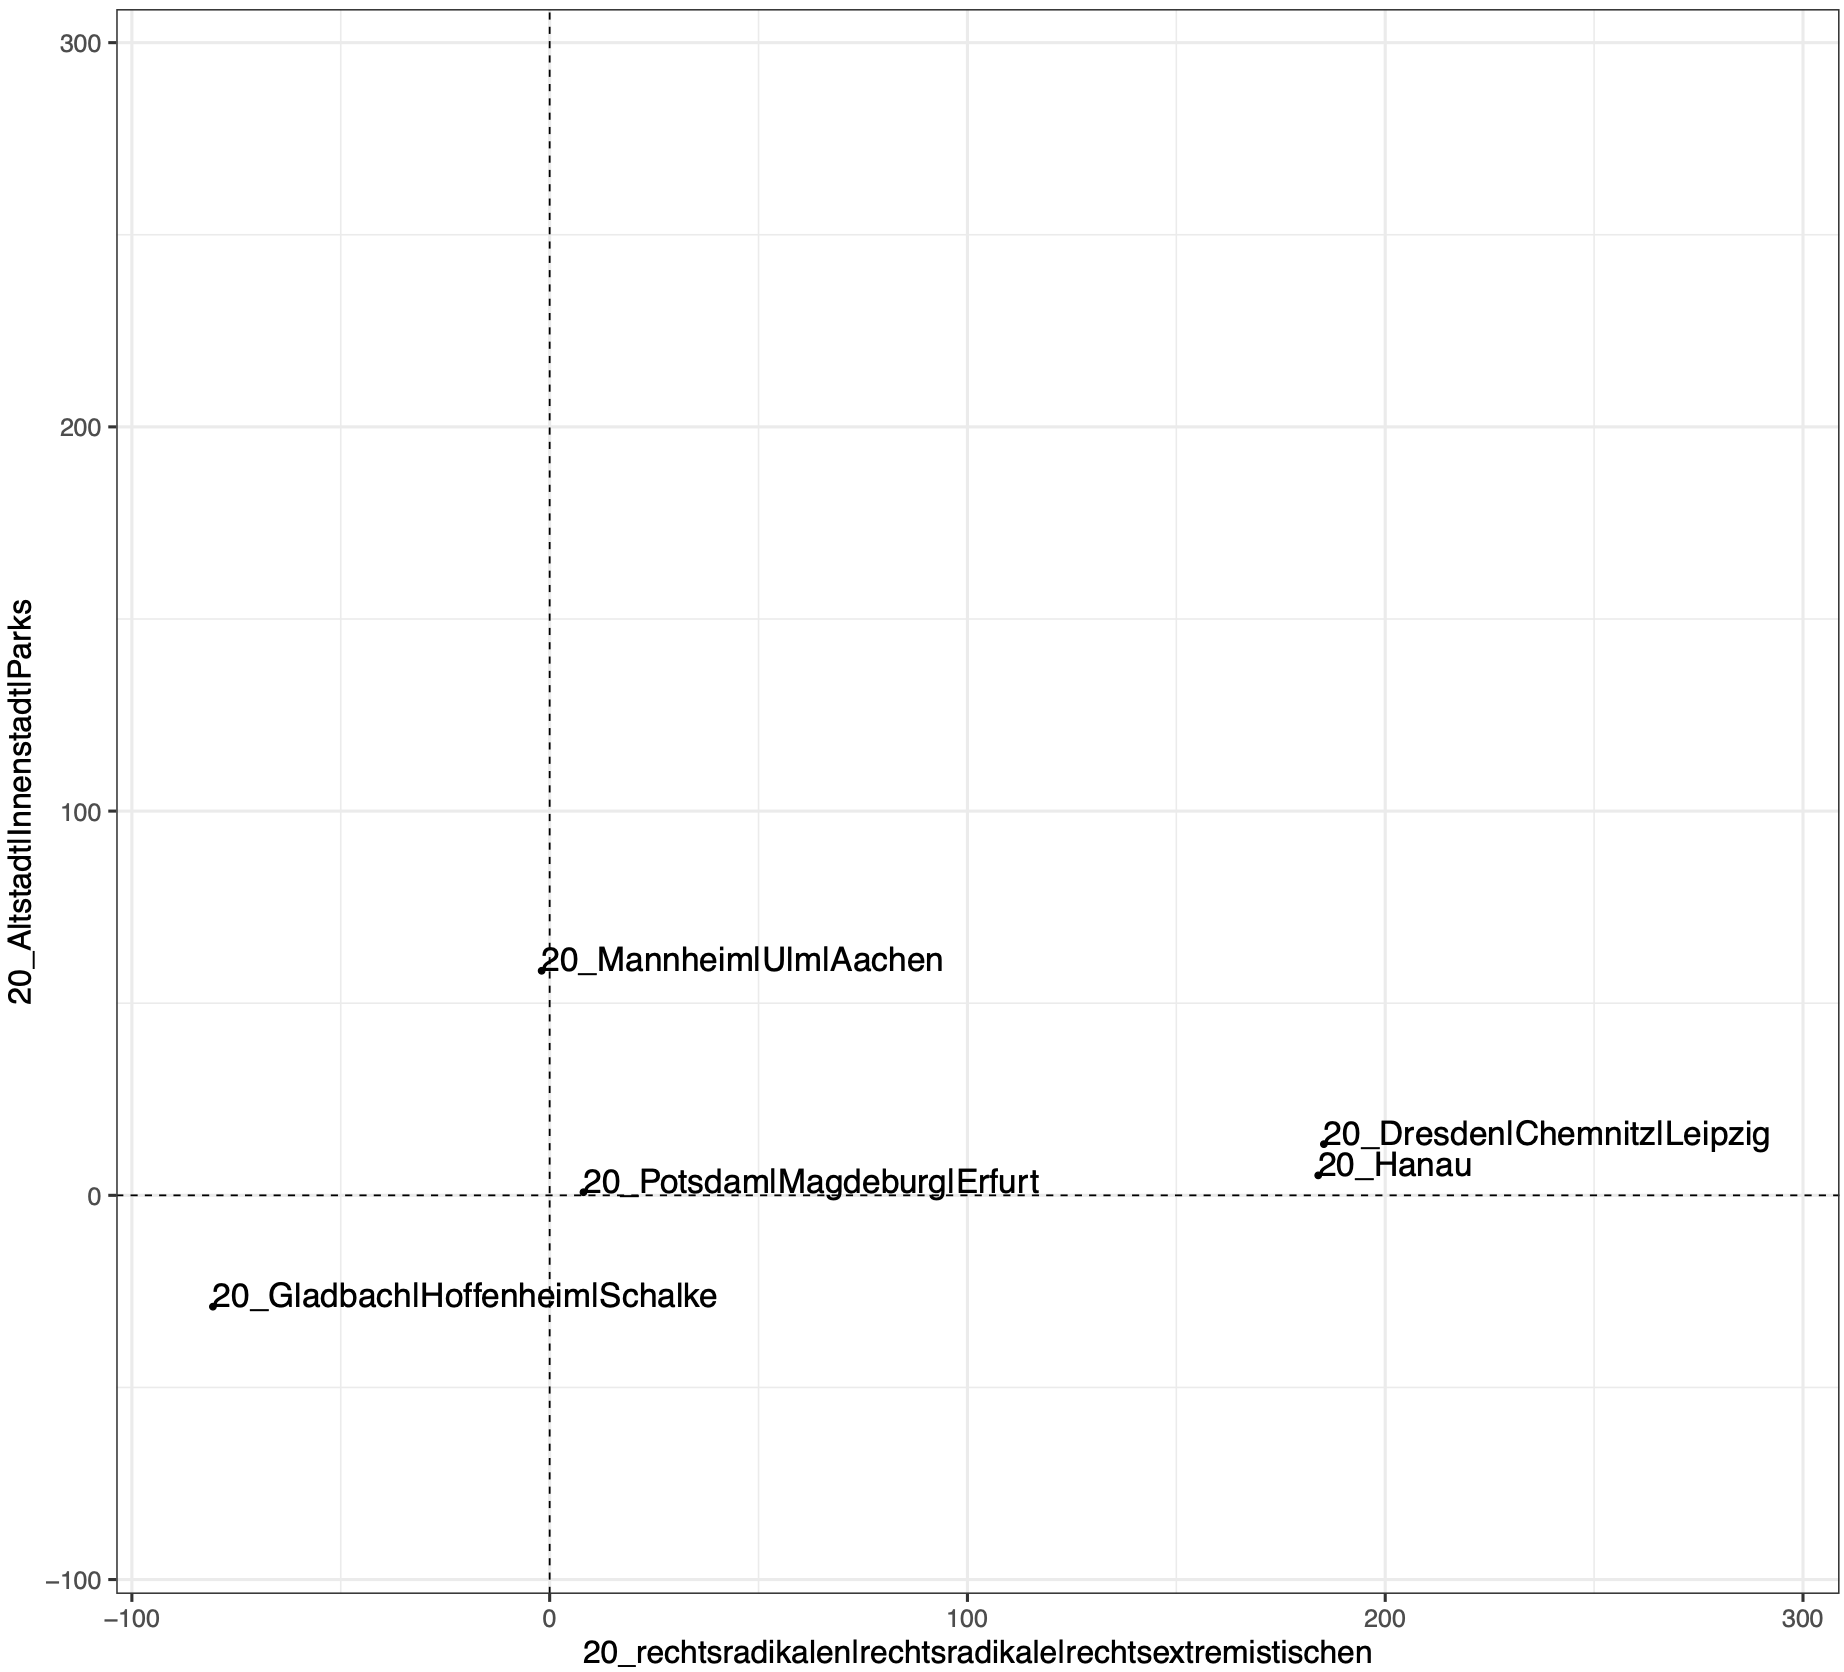
\includegraphics[width=\textwidth]{figures/media/image12.png}
  \caption{\label{fig:staedte-loglikelihood-cluster}Räumliche Darstellung der \emph{Log-Likelihood}-Werte der Städte im Verhältnis zu zwei Clustern aus \tabref{tab:collocation_matrix}.}
\end{figure}

Zu beachten ist, dass zur Messung der Distanz von Word Embeddings in der Regel die Cosinus-Distanz verwendet wird, d.\,h. es wird der Winkel zwischen zwei Punkten im Vektorraum gemessen, nicht ihr ‚direkter` Abstand (euklidische Distanz). Das Cluster \cluster{20\_Potsdam{\breakbar}Magedburg{\breakbar}Erfurt} ist also nur im Sinne der euklidischen Distanz näher an \cluster{20\_Gladbach{\breakbar}Hoffenheim{\breakbar}Schalke} als an \cluster{20\_Hanau} und \cluster{20\_Dresden{\breakbar}Chemnitz{\breakbar}Leipzig}.\footnote{Es sei außerdem noch einmal betont, dass diese Ausführungen nur illustrativen Charakter haben. Zwar approximieren auf klassischen Kollokationen (PMI) beruhende Vektoren durchaus W\emph{ord2Vec}-Skip-Gram-Vektoren \autocite{levyNeuralWordEmbedding2014}. Die tatsächliche Berechnung von neuronalen Word Embeddings, wie in der folgenden Analyse vorgenommen, unterscheidet sich jedoch wesentlich (siehe Kapitel \ref{wie-funktioniert-die-berechnung-von-word-embeddings}).} Misst man hingegen die Cosinus-Distanz, sind sich die Cluster \cluster{20\_Potsdam{\breakbar}Magedburg{\breakbar}Erfurt}, \cluster{20\_Hanau} und \cluster{20\_Dresden{\breakbar}Chemnitz{\breakbar}Leipzig} sehr nahe, da ihre Vektoren vom Koordinatenursprung aus in eine ähnliche Richtung zeigen, während das Cluster \cluster{20\_Gladbach{\breakbar}Hoffenheim{\breakbar}Schalke} von ihnen am weitesten entfernt ist.

Betrachtet man Nachbarschaften von Wörtern im Vektorraum, wird die paradigmatische Relation, die Distanzen in ebendiesem zugrunde liegt, deutlich. So sind die nächsten Nachbarn zum Wort \emph{gesund} im Teilkorpus 2020--2021 etwa \emph{fit}, \emph{krank}, \emph{topfit}, \emph{symptomfrei} und \emph{wohlauf}, also Wörter, die in einer teilsynonymen oder antonymen Beziehung zum Ausgangswort stehen. Was an diesem Beispiel ebenfalls deutlich wird, ist der Einfluss des Korpus, auf dem die Embeddings trainiert wurden. So ist \emph{symptomfrei} im vorigen Zeitraum 2017--2019 nicht unter den nächsten Nachbarn des Wortes, dafür finden sich die Ausdrücke \emph{ungesund}, \emph{schmerzfrei}, \emph{gesünder}, \emph{hungrig} und \emph{fit} als fünf nächste Nachbarn, was anzeigt, dass es hier viel mehr um Fragen des \emph{gesunden} Lebensstils bzw. anderersartige Krankheiten (\emph{schmerzfrei}) geht als während der Corona-Pandemie. Word Embeddings repräsentieren also nicht einfach eine kontextabstrakte Bedeutung im Sinne einer lexikalischen Semantik, die pragmatische Aspekte ausklammert. Während es sinnvoll erscheinen könnte, sehr große und in Hinblick auf unterschiedliche Strata ausgewogene Referenzkorpora zu verwenden, um solche kontextuellen semantischen Verschiebungen zu nivellieren, ist dies gerade in korpuspragmatischen Ansätzen nicht sinnvoll. Word Embeddings stellen hier, gerade weil sich Kontexte in sie einschreiben, ein hervorragendes Mittel dar, um kontextbedingte diskursive Veränderungen -- operationalisiert als Subkorpora -- analysieren zu können. Unterschiede, die sich durch die Wahl des Korpus bzw. Subkorpus ergeben, sind hier also kein Stichprobenproblem, sondern intendierte Datengrundlage für die Analyse \autocite[siehe auch][217-218]{knuchelMachineLearningUnd2023}.

Mithilfe von Word-Embeddings gelingt es also, einen von Tognini-Bonelli zentral gesetzten methodischen Schritt des \emph{corpus-driven} Vorgehens systematisch für jeden Type des Korpus durchzuführen, nämlich die Analyse von Konkordanzen auf der vertikalen Achse in Hinblick auf Muster (hier: im Kotext vorkommende Wörter) und diese nur in der Zusammenschau ersichtlichen Muster als für das Sprachsystem unmittelbar relevant zu deuten:

\begin{quote}
The patterns on the vertical axis are the patterns of \emph{langue} and these are just as physical and concrete as those of \emph{parole}, but they could not be observed until the instances were gathered together - until the advent of computer corpora. The theorists of the earlier part of last century thought that the organisation of \emph{langue} was abstract and unobservable, but that position was an indication of the state of the technology and not the state of the language. The \emph{langue} of Italian, as it relates to the profile of \emph{saper} and of \emph{sapere}, for instance, is there on the page, every bit as physically present as each of its component utterances. \autocite[98-99]{tognini-bonelliCorpusLinguisticsWork2001}
\end{quote}

Im Vergleich zum Vorgehen bei Tognini-Bonelli, das noch auf der Betrachtung von Konkordanzlisten zu einzelnen Suchanfragen beruhte, hat die Technologie nun erneut einen großen Schritt gemacht und das Type-Inventar ganzer Korpora kann auf syntagmatische Gebrauchsmuster untersucht werden.

\subsubsubsection{Wie funktioniert die Berechnung von Word Embeddings?}\label{wie-funktioniert-die-berechnung-von-word-embeddings}

% Zum Durchbruch verhalfen Word Embeddings die von Mikolov et al. \autocite*{mikolovEfficientEstimationWord2013} bei Google entwickelten \emph{Word2Vec}-Algorithmen, mit denen die Ermittlung der Vektoren effizient und für große Datenmengen mit überschaubarem Hardware-Bedarf möglich wurde. Dabei wird ein neuronales Netz verwendet, mit dessen Hilfe Embeddings mit üblicherweise zwischen 200 und 600 Dimensionen berechnet werden können. Die Anzahl der Dimensionen liegt hier also deutlich unter der des oben zu Zwecken der Illustration skizzierten Beispiels, das die gesamte Type-Anzahl des Korpus als Dimensionen erfordern würde. Die Kehrseite dieses effizienteren Verfahrens ist, dass die einzelnen Werte der Dimensionen nicht unmittelbar interpretierbar sind. Sie stellen nun statt konkreten \emph{latente} semantische Features dar. Eine einzelne Dimension kann also etwas über das Kollokationsverhalten mit einer ganzen (unbekannten) Reihe anderer Wörter aussagen. Die Funktionsweise des neuronalen Netzes im Fall von \emph{Word2Vec} \autocite{mikolovEfficientEstimationWord2013} soll im Folgenden skizziert werden \autocite[siehe ausführlich][]{rongWord2vecParameterLearning2016}. Zunächst ist zwischen zwei Varianten des Algorithmus zu unterscheiden: \emph{Continuous Bag of Words} (CBOW) und \emph{Continuous Skip-gram} (Skip-Gram). Für beide Algorithmen wird das Korpus zunächst tokenisiert und in Sätze gegliedert. Im Anschluss erfolgt ein Training des neuronalen Netzes, indem es Vorhersagen über die Wörter im Satz -- in Abhängigkeit der sie umgebenden Wörter -- treffen muss. Während das Training neuronaler Netze in der Regel ein Trainingsdatenset voraussetzt, in dem die zu lernenden Features bereits (oftmals händisch) annotiert sind, nutzen Word-Embedding-Algorithmen das Korpus selbst als Trainingsgrundlage. Sie maskieren einzelne Wörter und sagen sie in Abhängigkeit anderer sie umgebender Wörter voraus -- kennen dabei ja aber stets die richtige Antwort und können so den Erfolg ihrer Vorhersage bewerten. Im Fall von CBOW wird ein Wort des Satzes maskiert und das Netz muss auf Basis des Kotextes (ein festzulegender Wert von per Default zwei Wörtern zur Linken und Rechten des Fokus-Wortes) vorhersagen, um welches Wort es sich handelt. Bei \emph{SkipGram} wird umgekehrt ein Wort vorgegeben und die Vorhersage erfolgt zum maskierten Kontext. Wesentliche Parameter für den Algorithmus sind die Anzahl der Dimensionen, die Variante (CBOW oder \emph{SkipGram}) und das Kontextfenster. Die Architektur des verwendeten neuronalen Netzes (siehe \figref{fig:cbow-architektur}) umfasst eine Eingabeschicht (\emph{input layer}), eine interne Repräsentation (\emph{projection layer}) sowie eine Ausgabeschicht (\emph{output layer}). Alle \emph{layer} entsprechen Vektoren einer bestimmten Länge und beinhalten Zahlenwerte. \emph{In}- und \emph{output layer} haben die Länge des Korpusvokabulars, während die Länge des \emph{projection layers} der festzulegenden Dimensionsanzahl entspricht.
%
% \begin{figure}[t]
%   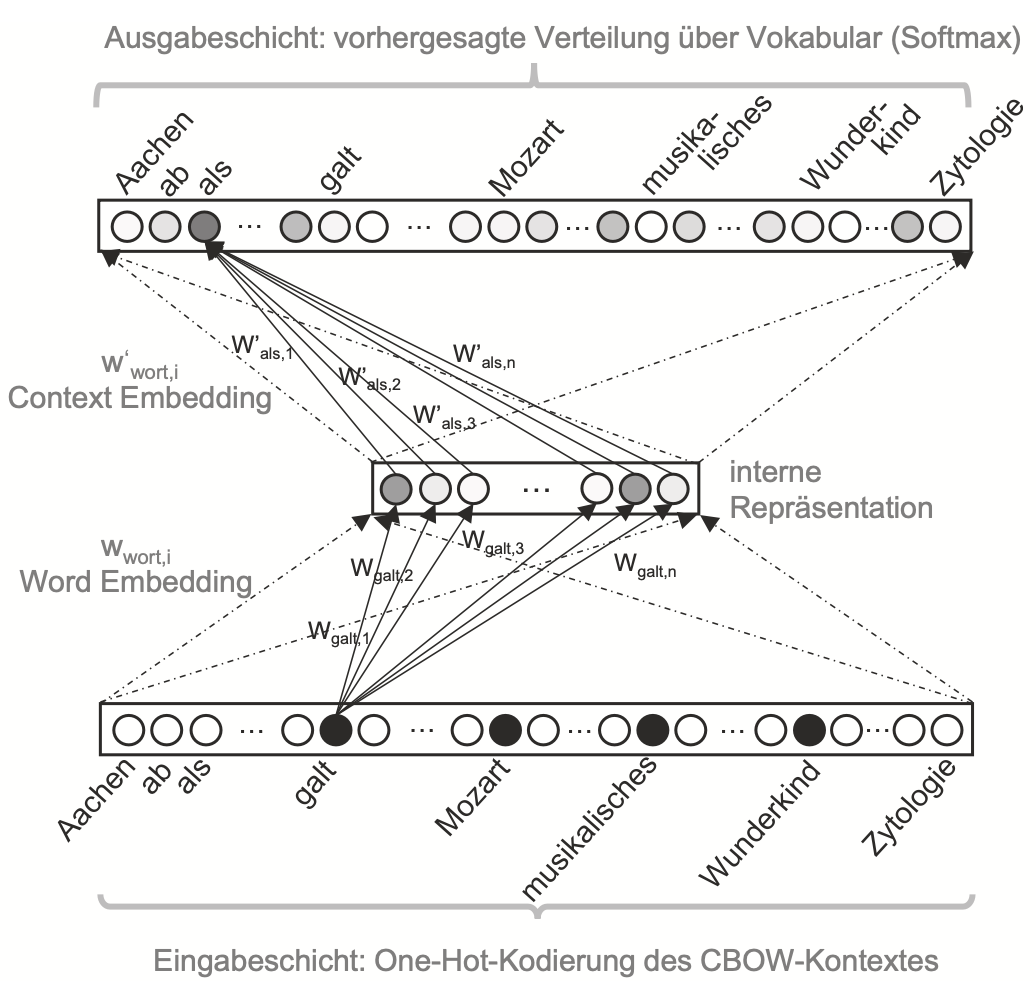
\includegraphics[width=\textwidth]{figures/media/image13.png}
%   \caption{\label{fig:cbow-architektur}Schematische Darstellung der CBOW-Architektur für die Vorhersage von \emph{als} im Satz \emph{Mozart galt als musikalisches Wunderkind} (Abbildung 5.11 aus \citealt[221]{biemannWissensrohstoffTextEinfuehrung2022}).}
% \end{figure}
%
% ~\figref{fig:cbow-architektur} zeigt eine schematische Darstellung für die CBOW-Variante des Algorithmus. Im unteren \emph{input layer} ist ausschnittsweise ein Vektor der Länge des Korpusvokabulars dargestellt, in dem die vier Kontextwörter \emph{galt}, \emph{Mozart}, \emph{musikalisch} und \emph{Wunderkind} markiert sind. Genau genommen verbergen sich dahinter vier Vektoren, jeweils in der Länge des Korpusvokabulars, die an jeder Stelle des Vokabulars eine 0 aufweisen, außer an der Stelle des jeweiligen Kontext-Wortes, das mit 1 markiert ist (sogenannte \emph{One-Hot}-Vektoren). Es finden im Anschluss in zwei Schritten Matrix-Multiplikationen statt: Zunächst wird jeder der vier \emph{One-Hot}-Vektoren mit \emph{n} zufällig initialisierten Werten, den sogenannten Gewichten, multipliziert und das arithmetische Mittel dieser vier Matrix-Multiplikationen (die ‚latente` oder ‚interne Repräsentation`) vom \emph{projection layer} in Richtung \emph{output layer} weitergegeben. Es findet nun erneut eine Matrix-Multiplikation mit zufällig initialisierten Werten statt. Dieses Mal entspricht die Anzahl der Gewichte jedoch der Größe des Vokabulars, d.\,h. der Anzahl der Korpus-Types. Das Ergebnis der Multiplikation sowie der nachfolgenden Anwendung der \emph{softmax}-Funktion\footnote{Mithilfe der \emph{softmax}-Funktion können die Werte von Vektoren in eine Wahrscheinlichhkeitsverteilung überführt werden.} findet sich im \emph{output layer}. Es handelt sich um einen Vektor der Länge des Vokabulars, wobei jeder Wert der Wahrscheinlichkeit des jeweiligen Wortes des Vokabulars in Abhängigkeit der Kontext-Wörter \emph{Mozart}, \emph{galt}, \emph{musikalisches} und \emph{Wunderkind} entspricht (das sogenannte \emph{context embedding}). Durch die dunkle Färbung der Vektordimension zu \emph{als} zeigt die Grafik an, dass das Training bereits fortgeschritten ist und das richtige Wort vorhergesagt wird. Der Ausgabevektor wird sodann mit dem Eingabevektor (Zielwort = 1, andere Wörter = 0) abgeglichen und die gemessene Differenz zwischen beiden zur Adjustierung der Gewichte genutzt (\emph{back propagation}). Während die \emph{context embeddings} i.d.R. nicht weiter genutzt werden,\footnote{Siehe aber z.\,B. Fankhauser \& Kupietz \autocite*{fankhauserCountBasedPredictiveLanguage2022}, die mit ihrer Hilfe Kollokationen \emph{prediction-} statt \emph{count-based} berechnen.} finden sich die eigentlichen \emph{n}-dimensionalen Word Embeddings in den Gewichten zwischen \emph{input} und \emph{projection layer}.
%
% \hspace{-1mm} Zu beachten bei der Berechnung bzw. der Interpretation von Word-Embedding-Modellen (WEM) ist, dass ein WEM immer nur in sich schlüssig ist und die Embeddings eines Modells nicht mit denen anderer, unabhängig trainierter, Modelle verglichen werden können. Dies liegt in den Zufallskomponenten begründet, die beim Training des neuronalen Netzes wirksam sind. Man spricht bei diesen Algorithmen von nicht-deterministischen Algorithmen. Im Gegensatz zu ihren deterministischen Äquivalenten liefern sie auch bei gleicher Datengrundlage und gleichen Parametern keine identischen Ergebnisse. Es ist außerdem wichtig, auf eine möglichst große Datengrundlage und mithin eine möglichst große Anzahl an Kotexten für jedes Wort zurückgreifen zu können, um Zufallseinflüsse zu mindern.

Zum Durchbruch verhalfen Word Embeddings die von Mikolov et al. \autocite*{mikolovEfficientEstimationWord2013} bei Google entwickelten \emph{Word2Vec}-Algorithmen, mit denen die Ermittlung der Vektoren effizient und für große Datenmengen mit überschaubarem Hardware-Bedarf möglich wurde. Dabei wird ein neuronales Netz verwendet, mit dessen Hilfe Embeddings mit üblicherweise zwischen 200 und 600 Dimensionen berechnet werden können. Die Anzahl der Dimensionen liegt hier also deutlich unter der des oben zu Zwecken der Illustration skizzierten Beispiels, das die gesamte Type-Anzahl des Korpus als Dimensionen erfordern würde. Die Kehrseite dieses effizienteren Verfahrens ist, dass die einzelnen Werte der Dimensionen nicht unmittelbar interpretierbar sind. Sie stellen nun statt konkreten \emph{latente} semantische Features dar. Eine einzelne Dimension kann also etwas über das Kollokationsverhalten mit einer ganzen (unbekannten) Reihe anderer Wörter aussagen. Die Funktionsweise des neuronalen Netzes im Fall von \emph{Word2Vec} \autocite{mikolovEfficientEstimationWord2013} soll im Folgenden skizziert werden \autocite[siehe ausführlich][]{rongWord2vecParameterLearning2016}. Zunächst ist zwischen zwei Varianten des Algorithmus zu unterscheiden: \emph{Continuous Bag of Words} (CBOW) und \emph{Continuous Skip-gram} (Skip-Gram). Für beide Algorithmen wird das Korpus zunächst tokenisiert und in Sätze gegliedert. Im Anschluss erfolgt ein Training des neuronalen Netzes, indem es Vorhersagen über die Wörter im Satz -- in Abhängigkeit der sie umgebenden Wörter -- treffen muss. Während das Training neuronaler Netze in der Regel ein Trainingsdatenset voraussetzt, in dem die zu lernenden Features bereits (oftmals händisch) annotiert sind, nutzen Word-Embedding-Algorithmen das Korpus selbst als Trainingsgrundlage. Sie maskieren einzelne Wörter und sagen sie in Abhängigkeit anderer sie umgebender Wörter voraus -- kennen dabei ja aber stets die richtige Antwort und können so den Erfolg ihrer Vorhersage bewerten. Im Fall von CBOW wird ein Wort des Satzes maskiert und das Netz muss auf Basis des Kotextes (ein festzulegender Wert von per Default fünf Wörtern zur Linken und Rechten des Fokus-Wortes) vorhersagen, um welches Wort es sich handelt. Bei \emph{SkipGram} wird umgekehrt ein Wort vorgegeben und die Vorhersage erfolgt zum maskierten Kontext. Wesentliche Parameter für den Algorithmus sind die Anzahl der Dimensionen, die Variante (CBOW oder \emph{SkipGram}) und das Kontextfenster. Die Architektur des verwendeten neuronalen Netzes (siehe \figref{fig:cbow-architektur}) umfasst eine Eingabeschicht (\emph{input layer}), eine interne Repräsentation (\emph{projection layer}) sowie eine Ausgabeschicht (\emph{output layer}). Alle \emph{layer} entsprechen Vektoren einer bestimmten Länge und beinhalten Zahlenwerte. \emph{In}- und \emph{output layer} haben die Länge des Korpusvokabulars, während die Länge des \emph{projection layers} der festzulegenden Dimensionsanzahl entspricht.

\begin{figure}[t]
  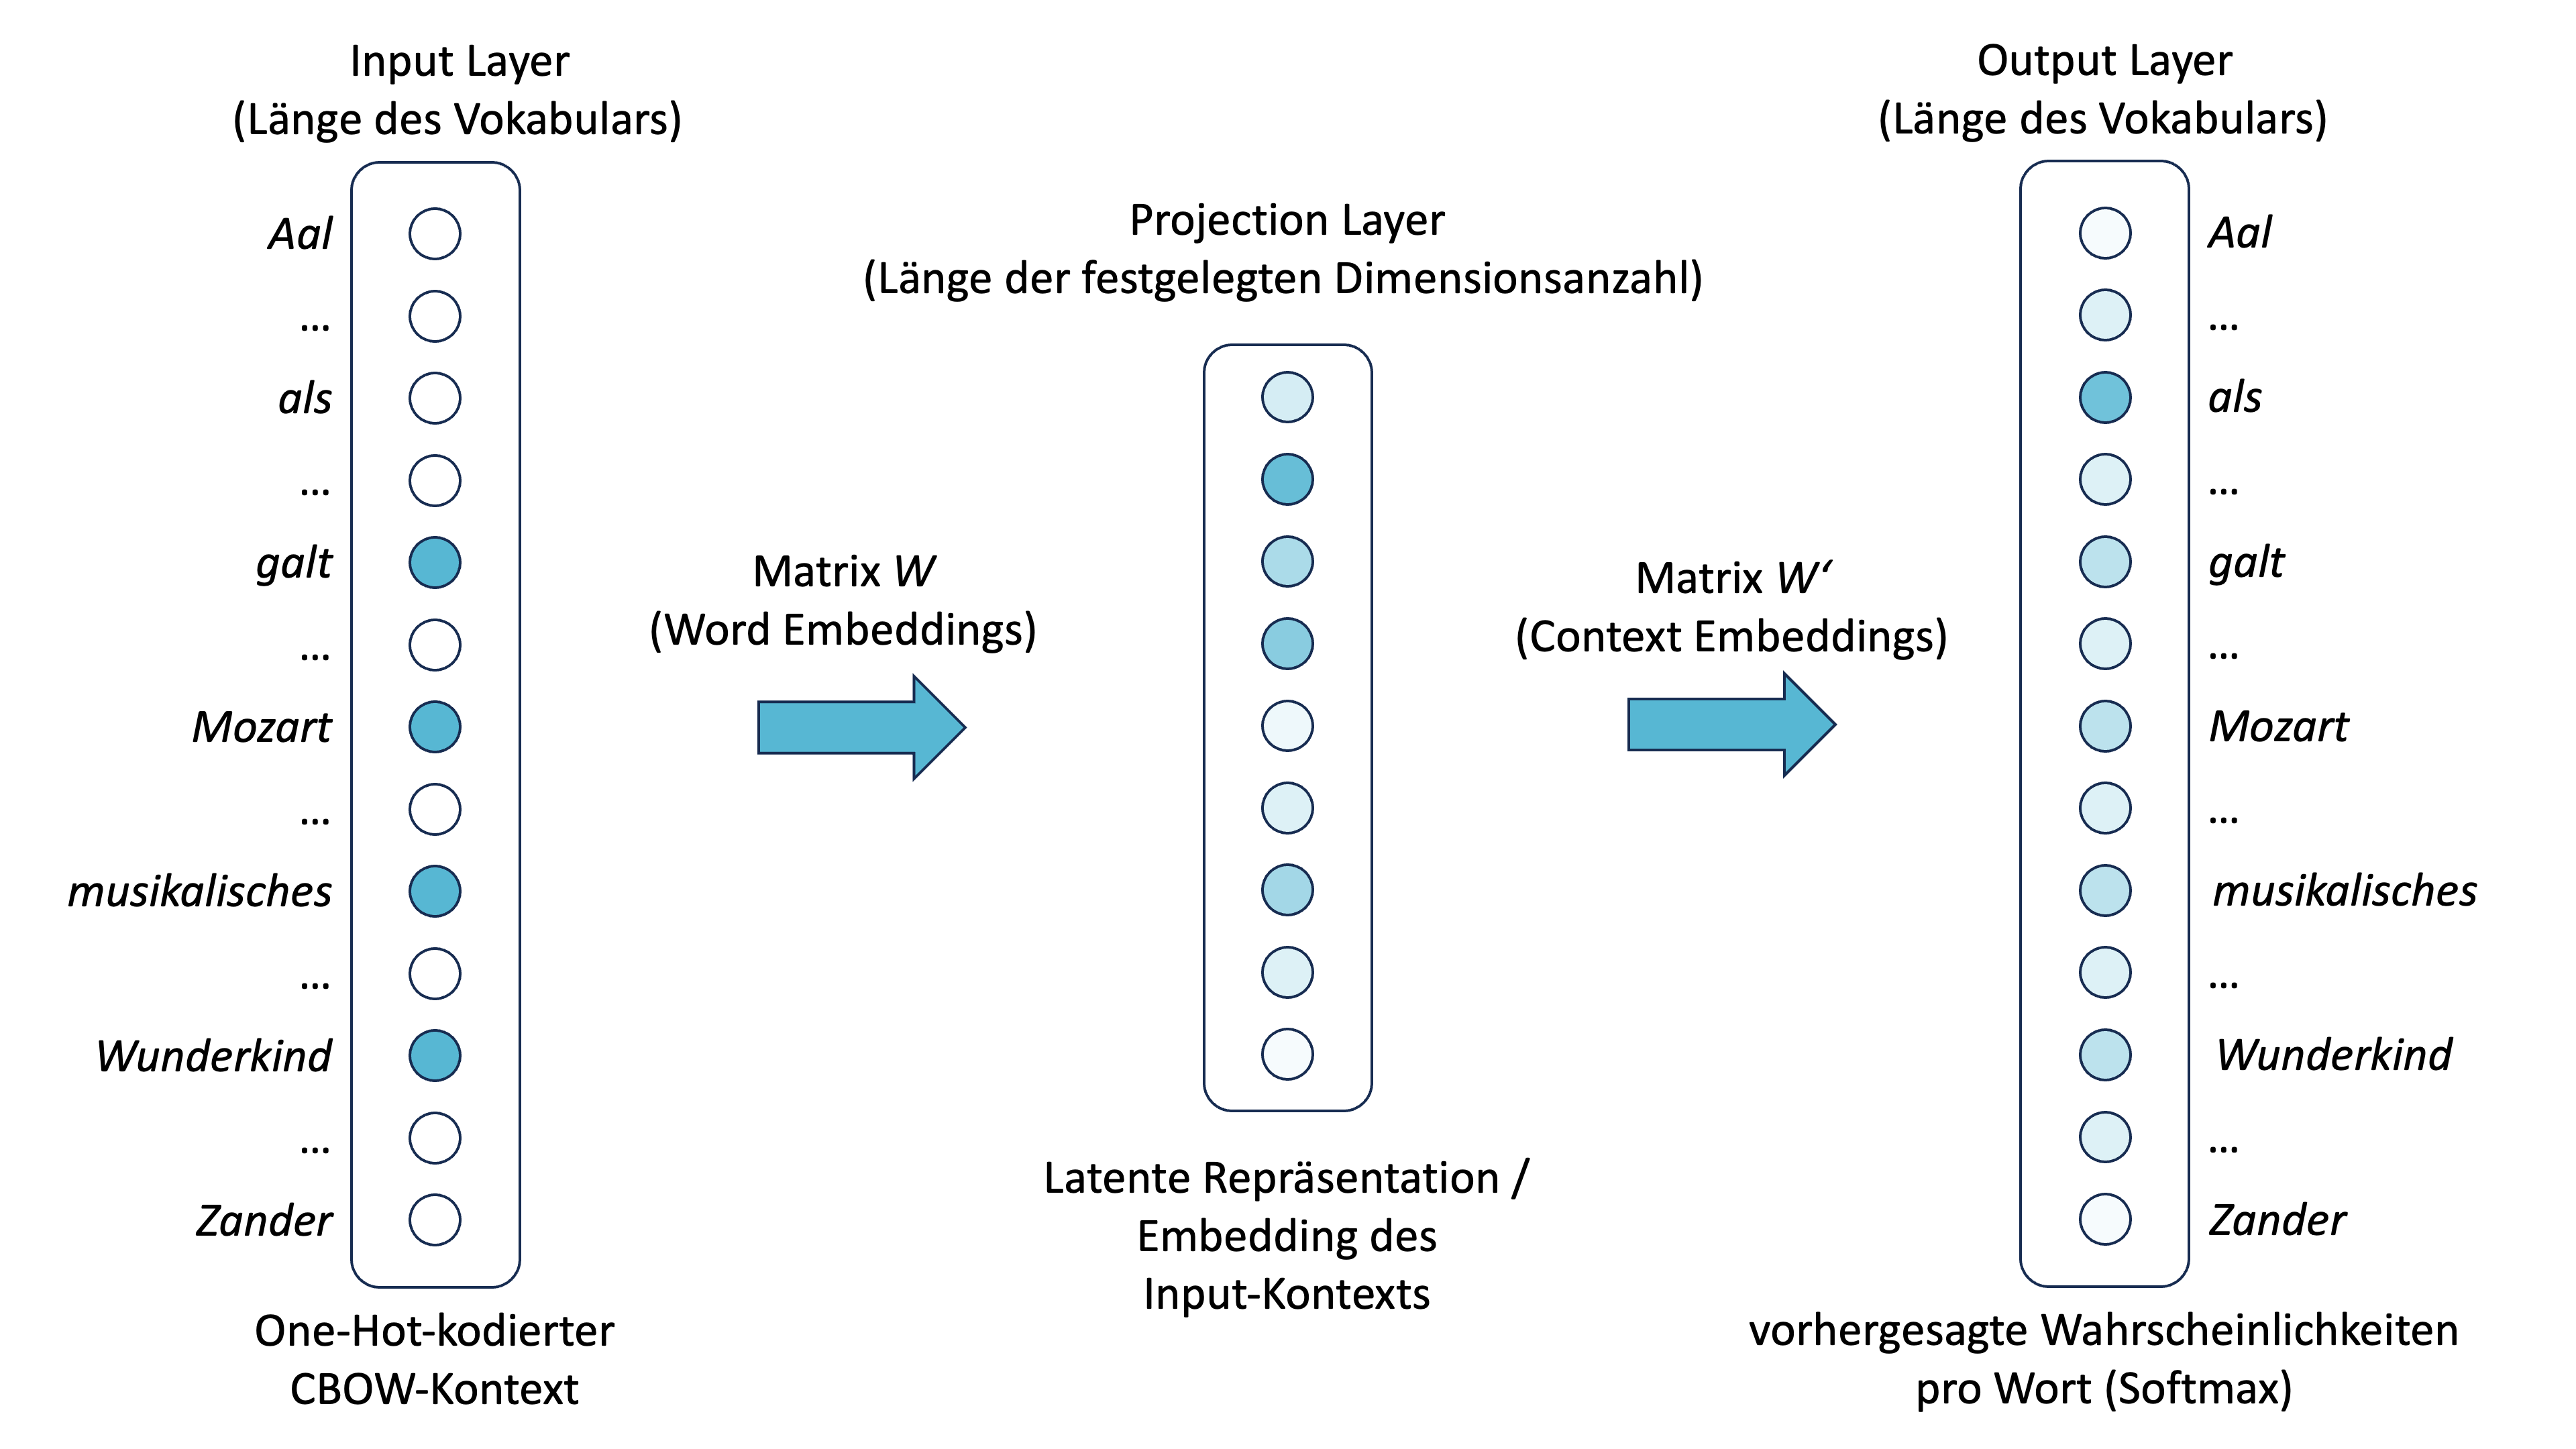
\includegraphics[width=\textwidth]{figures/media/grafik_cbow.png}
  \caption{\label{fig:cbow-architektur}Schematische Darstellung der CBOW-Architektur für die Vorhersage von \emph{als} im Satz \emph{Mozart galt als musikalisches Wunderkind} (Adaption von Abbildung 5.11 aus \citealt[221]{biemannWissensrohstoffTextEinfuehrung2022}).}
\end{figure}

~\figref{fig:cbow-architektur} zeigt eine schematische Darstellung für die CBOW-Variante des Algorithmus. Im unteren \emph{input layer} ist ausschnittsweise ein Vektor der Länge des Korpusvokabulars dargestellt, in dem die vier Kontextwörter \emph{galt}, \emph{Mozart}, \emph{musikalisch} und \emph{Wunderkind} markiert sind. Genau genommen verbergen sich dahinter vier Vektoren, jeweils in der Länge des Korpusvokabulars, die an jeder Stelle des Vokabulars eine 0 aufweisen, außer an der Stelle des jeweiligen Kontext-Wortes, das mit 1 markiert ist (sogenannte \emph{One-Hot}-Vektoren). Es finden im Anschluss in zwei Schritten Matrix-Multiplikationen (\emph{W} und \emph{W'}) statt: Zunächst wird jeder der vier \emph{One-Hot}-Vektoren mit \emph{n} zufällig initialisierten Werten, den sogenannten Gewichten, multipliziert und das arithmetische Mittel dieser vier Matrix-Multiplikationen (die ‚latente` oder ‚interne Repräsentation`) vom \emph{projection layer} in Richtung \emph{output layer} weitergegeben. Es findet nun erneut eine Matrix-Multiplikation mit zufällig initialisierten Werten statt. Dieses Mal entspricht die Anzahl der Gewichte jedoch der Größe des Vokabulars, d.\,h. der Anzahl der Korpus-Types. Das Ergebnis der Multiplikation sowie der nachfolgenden Anwendung der \emph{softmax}-Funktion\footnote{Mithilfe der \emph{softmax}-Funktion können die Werte von Vektoren in eine Wahrscheinlichhkeitsverteilung überführt werden.} findet sich im \emph{output layer}. Es handelt sich um einen Vektor der Länge des Vokabulars, wobei jeder Wert der Wahrscheinlichkeit des jeweiligen Wortes des Vokabulars in Abhängigkeit der Kontext-Wörter \emph{Mozart}, \emph{galt}, \emph{musikalisches} und \emph{Wunderkind} entspricht. Durch die dunkle Färbung der Vektordimension zu \emph{als} zeigt die Grafik an, dass das Training bereits fortgeschritten ist und das richtige Wort vorhergesagt wird. Der Ausgabevektor wird sodann mit dem Eingabevektor (Zielwort = 1, andere Wörter = 0) abgeglichen und die gemessene Differenz zwischen beiden zur Adjustierung der Gewichte genutzt (\emph{back propagation}). Während die \emph{context embeddings} i.d.R. nicht weiter genutzt werden,\footnote{Siehe aber z.\,B. Fankhauser \& Kupietz \autocite*{fankhauserCountBasedPredictiveLanguage2022}, die mit ihrer Hilfe Kollokationen \emph{prediction-} statt \emph{count-based} berechnen.} finden sich die eigentlichen \emph{n}-dimensionalen Word Embeddings in den Gewichten zwischen \emph{input} und \emph{projection layer}, d.h. in Matrix \emph{W}.

\hspace{-1mm} Zu beachten bei der Berechnung bzw. der Interpretation von Word-Embedding-Modellen (WEM) ist, dass ein WEM immer nur in sich schlüssig ist und die Embeddings eines Modells nicht mit denen anderer, unabhängig trainierter, Modelle verglichen werden können. Dies liegt in den Zufallskomponenten begründet, die beim Training des neuronalen Netzes wirksam sind. Man spricht bei diesen Algorithmen von nicht-deterministischen Algorithmen. Im Gegensatz zu ihren deterministischen Äquivalenten liefern sie auch bei gleicher Datengrundlage und gleichen Parametern keine identischen Ergebnisse. Es ist außerdem wichtig, auf eine möglichst große Datengrundlage und mithin eine möglichst große Anzahl an Kotexten für jedes Wort zurückgreifen zu können, um Zufallseinflüsse zu mindern.

\subsubsubsection{Vergleichbarkeit von Word-Embedding-Modellen}\label{vergleichbarkeit-von-word-embedding-modellen}

Um das Problem der Nicht-Vergleichbarkeit unabhängig trainierter Word-Embedding-Modelle zu lösen, wurden in der Computerlinguistik unterschiedliche Lösungsansätze entwickelt \autocites[siehe etwa][]{dubossarskyBottomApproachCategory2015, fankhauserAnalyzingDomainSpecific2019, yaoDynamicWordEmbeddings2018, dicarloTrainingTemporalWord2019}. Aufgrund der guten Performance-Werte sowie der einfachen Handhabbarkeit des Algorithmus verwende ich die Erweiterung des \emph{Word2Vec} Algorithmus \emph{Temporal Word Embeddings with a Compass} (TWEC) von Di Carlo et al. \autocite*{dicarloTrainingTemporalWord2019}, die das Training von WEM im gleichen Vektorraum für unterschiedliche Subkorpora erlaubt. Die Funktionsweise von TWEC lässt sich wie folgt skizzieren: Zunächst wird ein reguläres Word-Embedding-Modell (der sogenannte \emph{compass}) auf dem gesamten Korpus trainiert, wobei die CBOW-Variante von \emph{Word2Vec} zum Einsatz kommt. Im Anschluss wird die fertig trainierte zweite Matrix des neuronalen Netzes eingefroren und für das Training aller weiteren Modelle für Subkorpora desselben Korpus (sogenannte \emph{slices}) verwendet. Aktualisiert werden dabei dann nur noch die Gewichte zwischen \emph{input} und \emph{projection layer} was dazu führt, dass die resultierenden Wortvektoren zwar in den gleichen Vektorraum eingebettet, jedoch kontextspezifisch trainiert sind. \tabref{tab:diachronic_neighbors} führt die jeweils nächsten Nachbarn zu einzelnen Word Embeddings in unterschiedlichen mit TWEC berechneten diachronen Modellen auf. Fixiert ist jeweils der Ursprungskontext der Wörter. Es werden also z.\,B. in der ersten Zeile nicht die nächsten Nachbarn des Ausdrucks \emph{Querdenker} in den unterschiedlichen Teilkorpora abgefragt, was auch ohne alignierte Modelle möglich wäre, sondern die nächsten Nachbarn zu dem Punkt im semantischen Raum, an dem \emph{Querdenker} in den Jahren 1999--2001 lag. Es handelt sich also um eine onomasiologische statt einer semasiologischen Analyserichtung. Während sich diese Bedeutung kaum verändert hat -- es fällt allerdings auf, dass \emph{Querdenker} selbst im Jahr 2020--2021 nicht mehr an diesem Punkt auftaucht --, zeigt sich an der Abfrage des gleichen Wortes mit Ursprungskontext 2020--2021 ein gänzlich anderes Bild und mithin der Bedeutungswandel des Wortes in der Coronapandemie. Es wird ersichtlich, dass es mithilfe der Methode sehr gut gelingt, Bedeutungswandel einzelner Wörter zu erfassen. Es eröffnet sich zudem eine datengeleitete Zugriffsmöglichkeit auf dieses Phänomen, indem etwa im Vergleich zweier diachroner Word-Embedding-Modelle abgefragt werden kann, welche Wörter die größte Distanz im Vektorraum vom einen zum anderen Zeitpunkt zurückgelegt haben.

\begin{sidewaystable}\small
\caption{Nächste Nachbarn einzelner Embeddings mit Cosinus-Ähnlichkeit im zeitlichen Verlauf.}
\label{tab:diachronic_neighbors}
 \begin{tabularx}{\textwidth}{>{\hsize=0.8\hsize}Q >{\hsize=1.066\hsize}Q >{\hsize=1.066\hsize}Q >{\hsize=1.066\hsize}Q}
  \lsptoprule
  Ausgangsvektor & 1999--2001 & 2011--2013 & 2020--2021 \\
  \midrule
  \emph{Querdenker (99--01)} & \emph{Querdenker} (1.0), \emph{Pragmatiker} (0.73), \emph{Provokateur} (0.71), \emph{Selbstdarsteller} (0.69), \emph{Querkopf} (0.68) & \emph{Querdenker} (0.76), \emph{Netzwerker} (0.73), \emph{Freigeist} (0.70), \emph{Vordenker} (0.69), \emph{Pragmatiker} (0.69) & \emph{Pragmatiker} (0.66), \emph{Netzwerker} (0.66), \emph{Vordenker} (0.66), \emph{Liberaler} (0.65), \emph{Intellektueller} (0.64) \\
  \emph{Querdenker (20--21)} & \emph{Autonome} (0.75), \emph{Rechtsextreme} (0.70), \emph{Neonazis} (0.70), \emph{Rechtsextremen} (0.69), \emph{Rechtsradikale} (0.68) & \emph{Rechtsextreme} (0.73), \emph{Rechtsradikale} (0.71), \emph{Burschenschafter} (0.70), \emph{gewaltbereite} (0.70), \emph{Islamfeinde} (0.68) & \emph{Querdenker} (1.0), \emph{Coronaleugner} (0.80), \emph{Reichsbürger} (0.79), \emph{Corona-Leugner} (0.79), \emph{Impfgegner} (0.78) \\
  \emph{Hanau (20--21)} & \emph{Mölln} (0.63), \emph{Guben} (0.63), \emph{Rostock-lichtenhagen} (0.59), \emph{Solingen} (0.58), \emph{Düsseldorfer\_Synagoge} (0.57) & \emph{Mölln} (0.70), \emph{Solingen} (0.66), \emph{Rostock-lichtenhagen} (0.65), \emph{Newtown} (0.61), \emph{Lichtenhagen} (0.59) & \emph{Hanau} (1.0), \emph{Christchurch} (0.66), \emph{Mölln} (0.66), \emph{Hanauer} (0.64), \emph{Anschlag} (0.64) \\
  \emph{Björn\_Höcke (20--21)} & \emph{Christian\_Worch} (0.67), \emph{Horst\_Mahler} (0.65), \emph{NPD} (0.64), \emph{Aktionsbüro\_Norddeutschland} (0.63), \emph{Reps} (0.63) & \emph{Holger\_Apfel} (0.81), \emph{Udo\_Pastörs} (0.79), \emph{Udo\_Voigt} (0.77), \emph{Pastörs} (0.73), \emph{NPD-Kader} (0.72) & \emph{Björn\_Höcke} (1.0), \emph{Höcke} (0.88), \emph{Andreas\_Kalbitz} (0.85), \emph{Jörg\_Meuthen} (0.80), \emph{Thüringer\_AfD-Chef\_Björn\_Höcke} (0.79) \\
  \emph{Bin\_Laden (02--04)} & \emph{Bin\_Laden} (0.94), \emph{Osama\_Bin\_Laden} (0.90), \emph{Ussama\_Bin\_Laden} (0.87), \emph{bin\_Laden} (0.85), \emph{al-Qaida} (0.80) & \emph{Bin\_Laden} (0.86), \emph{bin\_Laden} (0.82), \emph{al-Qaida} (0.81), \emph{Osama\_Bin\_Laden} (0.76), \emph{Al-Qaida-Chef} (0.75) & \emph{al-Qaida} (0.69), \emph{Terroristen} (0.66), \emph{Soleimani} (0.64), \emph{iS} (0.64), \emph{Al-Qaida} (0.64) \\
  \lspbottomrule
 \end{tabularx}
\end{sidewaystable}

\subsubsubsection{Clustering von Word Embeddings}\label{clustering-von-word-embeddings}
\largerpage
Um Wörter nach ihrer paradigmatischen distributionellen Ähnlichkeit systematisch zusammenfassen und mithin FE induktiv erschließen zu können, bietet sich ein Clustering der berechneten Word Embeddings an, das in der Diskurslinguistik bereits erfolgreich angewandt wurde (siehe \chapref{distributionell-semantische-methodik}). Zum Clustering von Vektoren steht eine Vielzahl unterschiedlicher Algorithmen bereit, die jeweils unterschiedliche Vor- und Nachteile in Hinblick auf die bearbeitbare Datenmenge, die Laufzeit des Algorithmus, oder die Notwendigkeit, eine bestimmte Cluster-Anzahl vorab festzulegen, bieten.\footnote{Eine anschauliche Übersicht zu unterschiedlichen Clustering-Algorithmen steht unter \url{https://scikit-learn.org/stable/modules/clustering.html} zur Verfügung {[}18.12.2025{]}.} Gerade aus einer datengeleitet-explorativen Perspektive sind auch hierarchische Clustering-Algorithmen und solche, die keine vordefinierte Anzahl von Clustern benötigen und die Datenpunkte automatisch in Cluster sowie \emph{noise} gliedern, wie z.\,B. HDBSCAN \autocite{campelloDensityBasedClusteringBased2013} interessant. Mit ihnen wurde experimentiert, letztlich wurde jedoch aufgrund der großen Anzahl zu verarbeitender Datenpunkte (bis zu 365\,815 Types im \textsc{Taz}-Subkorpus) entschieden, den \emph{k-Means}-Algorithmus \autocite{macqueenMethodsClassificationAnalysis1967} zu verwenden, der große Datenmengen effizient in eine festgelegte Anzahl von \emph{k} Clustern einteilen kann und sich auch in Bubenhofers Analysen (siehe \chapref{distributionell-semantische-methodik}) bewährt hat. Bei einem \emph{k-Means}-Clustering wird jeder Datenpunkt, d.\,h. jedes Word Embedding, einem einzigen Cluster zugeordnet. Eine vorherige inhaltliche Definition der zu erwartenden Cluster ist jedoch nicht nötig; die Cluster-Erkennung erfolgt allein aufgrund der Verteilung der Datenpunkte, es handelt sich also um einen unüberwachten -- aus korpuslinguistischer Perspektive also \emph{corpus-driven} -- Algorithmus. Die Funktionsweise ist vergleichsweise simpel: Bei der Berechnung werden zunächst \emph{k} zufällige Cluster-Mittelpunkte (Centroids) im Vektorraum festgelegt. Danach werden alle Datenpunkte ihrem nächsten Cluster-Centroid zugeordnet und es wird pro Cluster aus allen zugeordneten Datenpunkten ein neuer Mittelpunkt berechnet. Im Anschluss beginnt der Prozess von vorne und es werden erneut alle Datenpunkte zugeordnet sowie daraufhin neue Centroids berechnet. Der Algorithmus endet, sobald sich die Zuordnung der Datenpunkte zu den Clustern nicht mehr oder nur noch geringfügig ändert. \figref{fig:kmeans-beispiel-k2} illustriert den Algorithmus an einem Beispiel.

\begin{figure}[t]
%   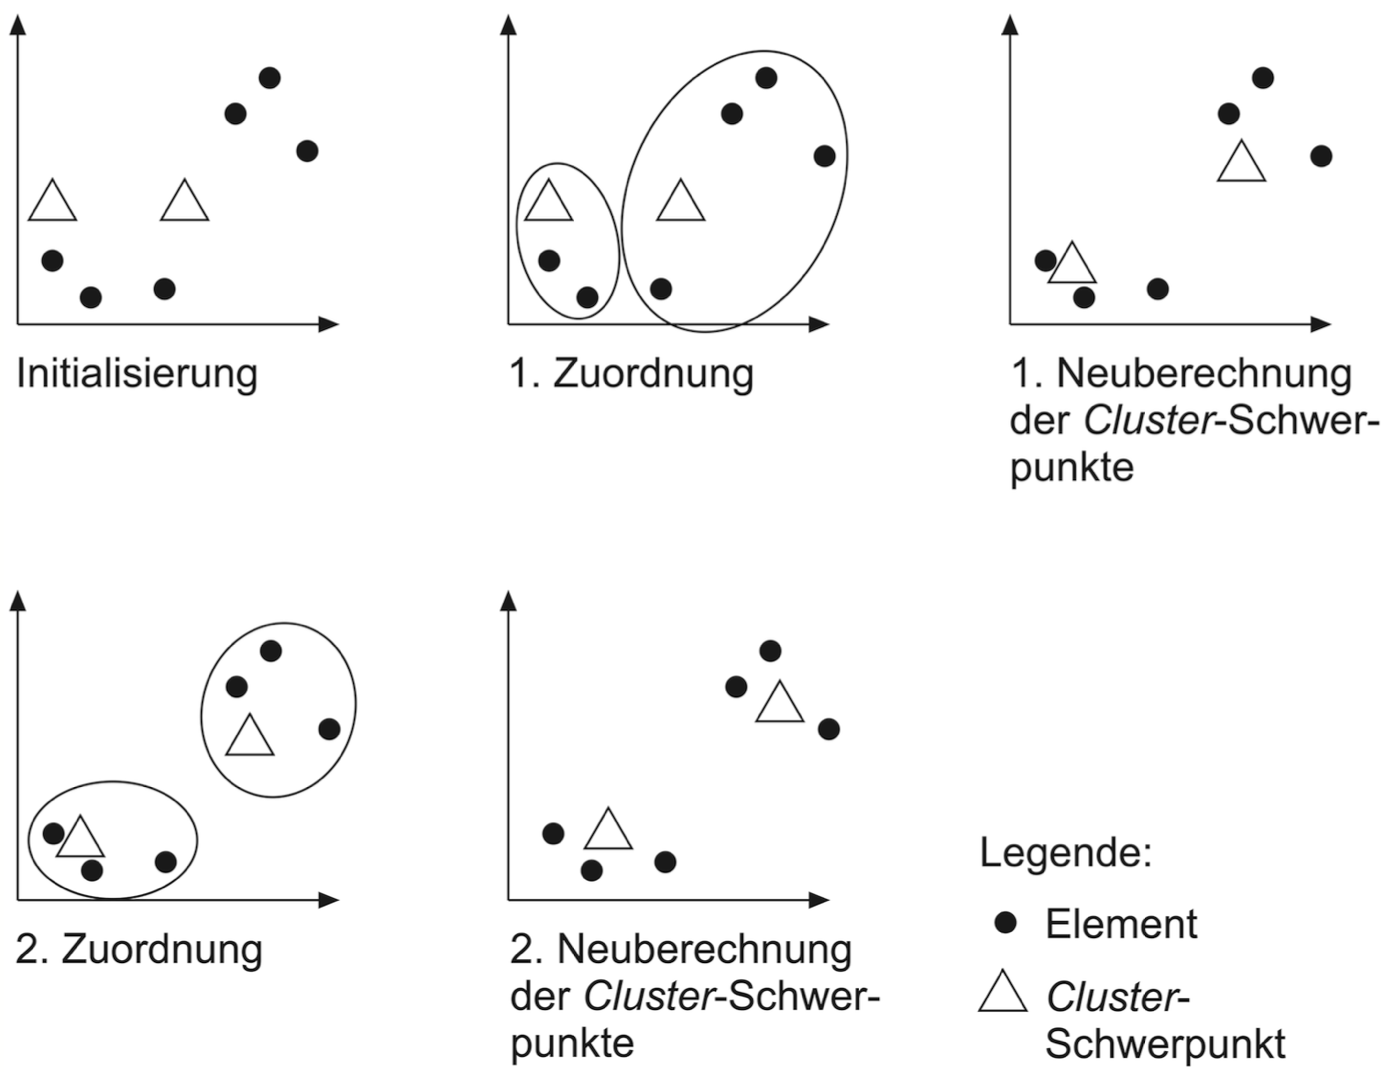
\includegraphics[width=\textwidth]{figures/media/image14.png}
%   \caption{\label{fig:kmeans-beispiel-k2}Illustration des \emph{k-Means}-Algorithmus bei \emph{k} = 2 und sechs Vektoren (Abbildung 6.5 aus \citealt[270]{biemannWissensrohstoffTextEinfuehrung2022}).}
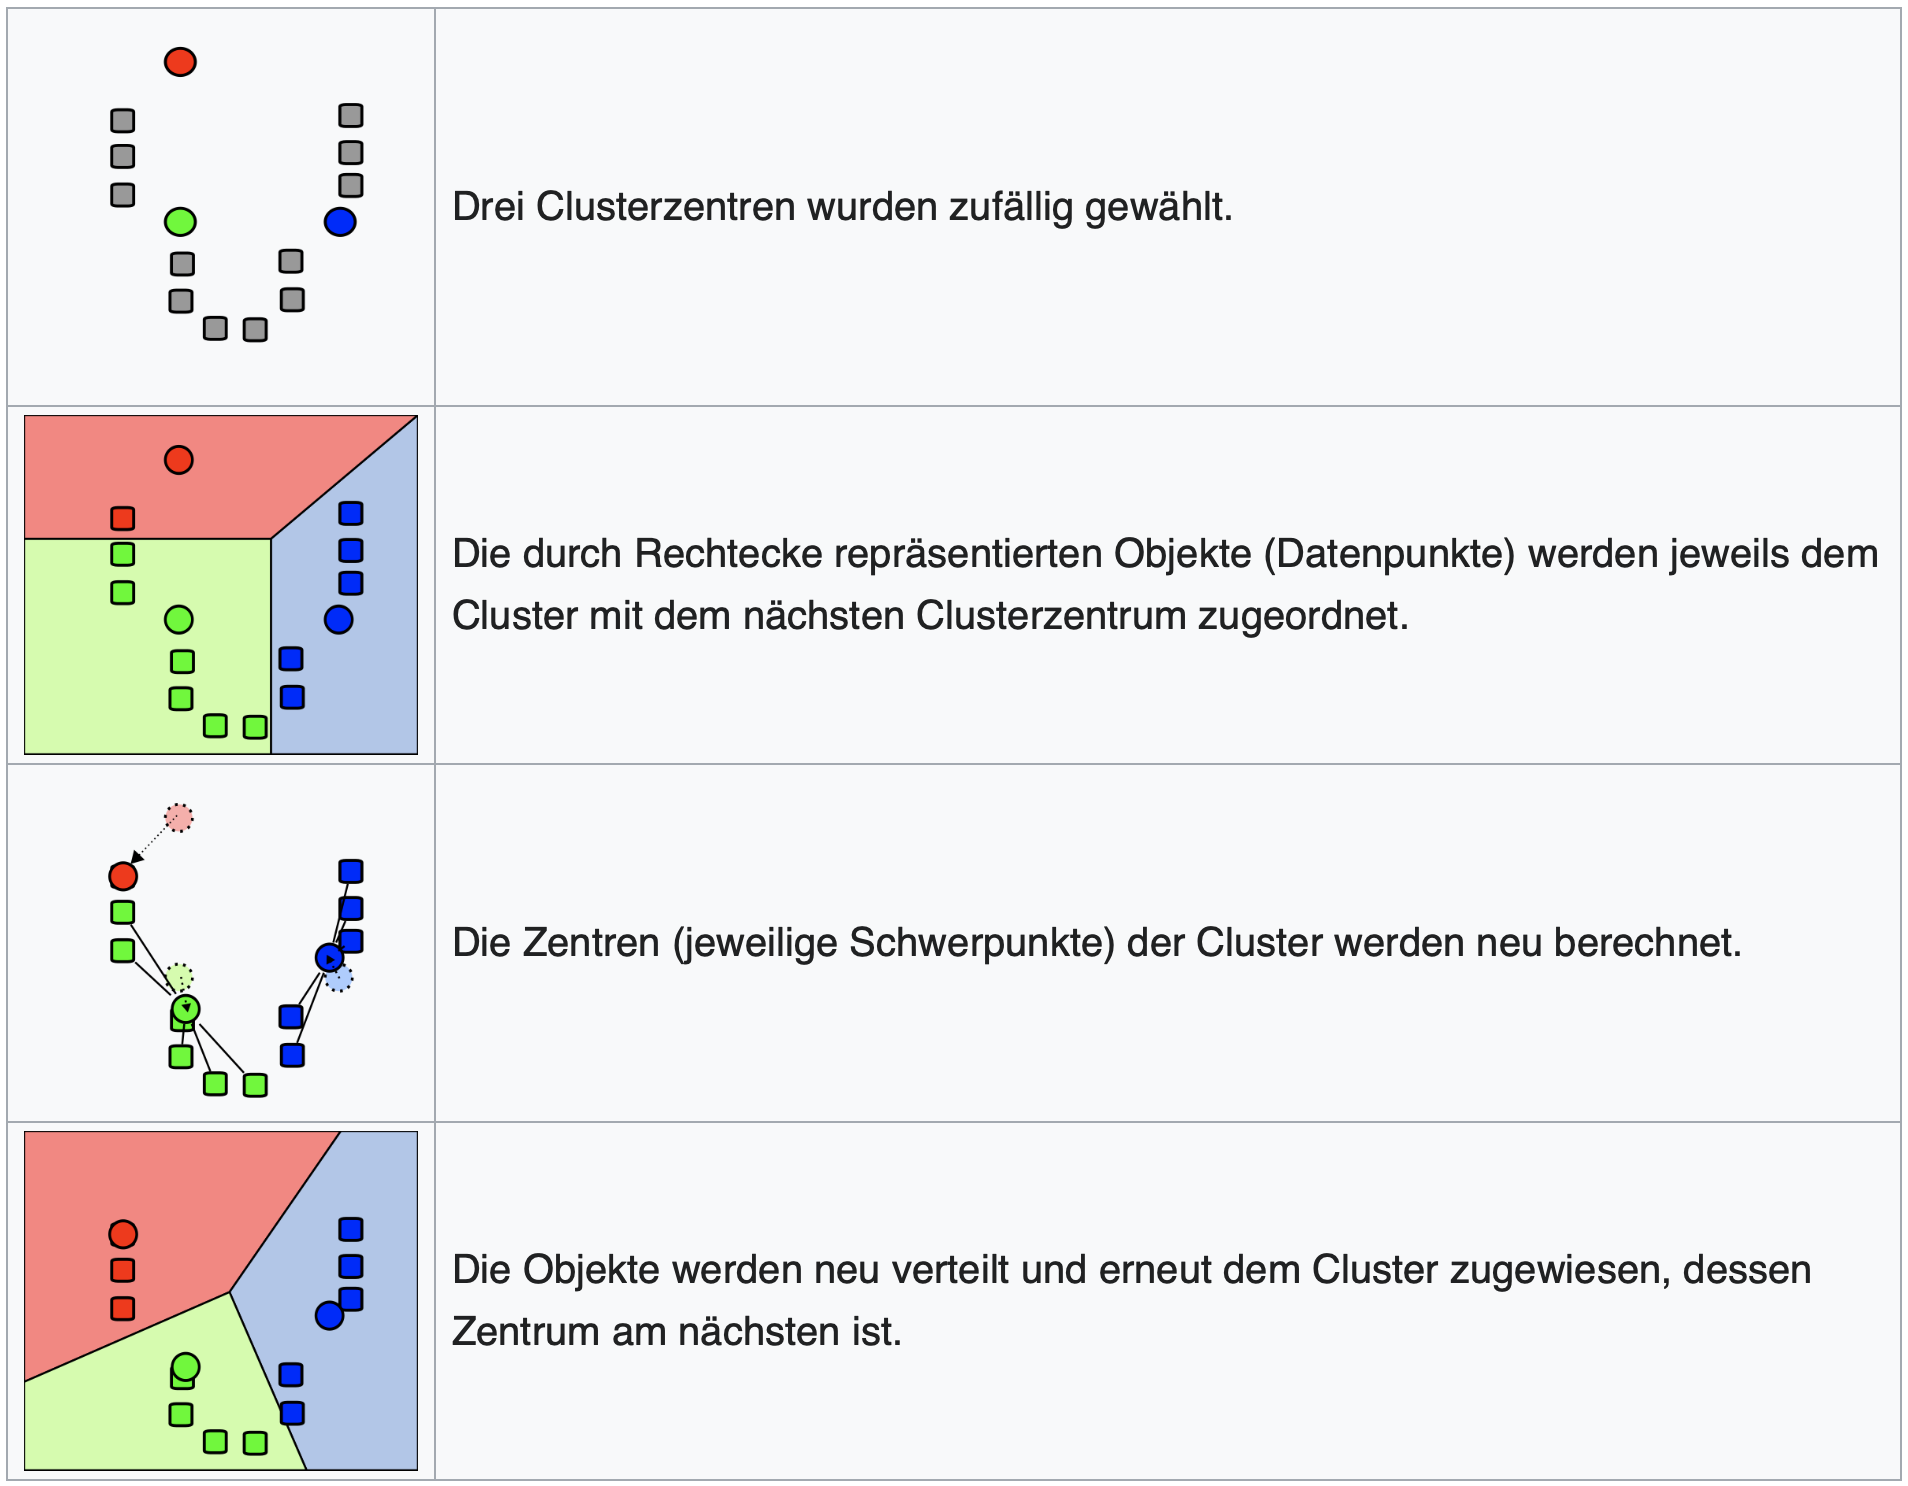
\includegraphics[width=\textwidth]{figures/media/kmeans.png}
  \caption{\label{fig:kmeans-beispiel-k2}Illustration des \emph{k-Means}-Algorithmus bei \emph{k} = 3 und zwölf Vektoren (Urheber der Grafiken: weston.pace, CC BY-SA 3.0, \url{https://de.wikipedia.org/wiki/K-Means-Algorithmus} [31.01.2026]).}
\end{figure}

\largerpage
Durch die Zufallskomponente bei der Initialisierung handelt es sich auch bei \emph{k-Means} um einen nicht-deterministischen Algorithmus, sodass die Zuordnungen der Wörter zu Clustern im Verlauf mehrerer Ausführungen variieren kann. Zu beachten ist darüber hinaus, dass wie Grand et al. \autocite*{grandSemanticProjectionRecovers2022} hervorheben, Nähe von Word Embeddings im Vektorraum immer auf einer globalen semantischen Ähnlichkeit beruht, die sich eigentlich in die Positionierung entlang einer Vielzahl semantischer Dimensionen aufspalten ließe. Je nachdem, was als \emph{tertium comparationis} gewählt ist, können also unterschiedliche Nachbarschaften von Wörtern entstehen. So weisen die Wörter \emph{dolphin} und \emph{tiger} eine geringe Distanz auf, wenn man sie auf die Dimension \emph{size} projiziert; jedoch eine große Distanz bei Projektion auf die Dimension \emph{danger} (siehe \emph{Figure 2a} in \citealt{grandSemanticProjectionRecovers2022}).

%
% \begin{figure}
%   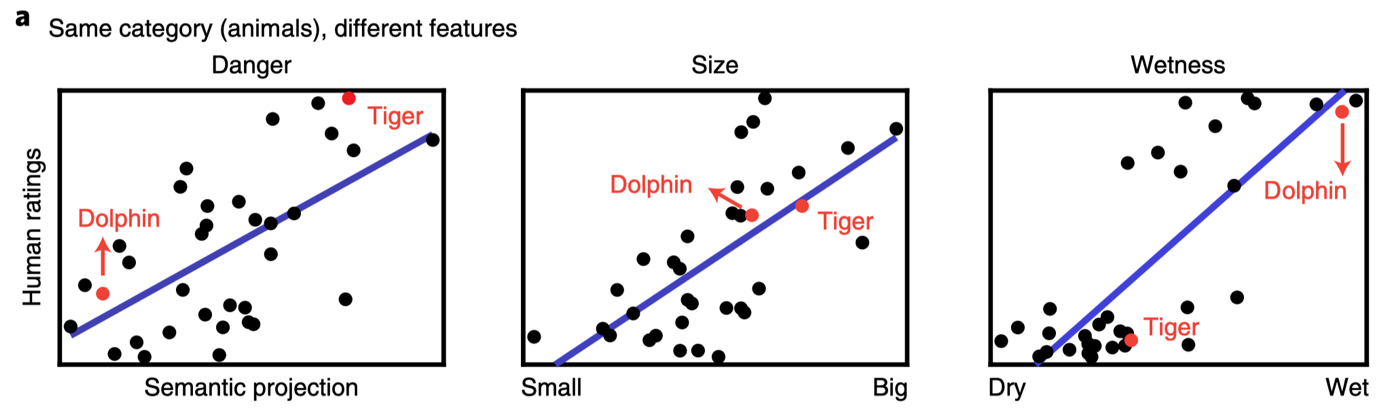
\includegraphics[width=\textwidth]{figures/media/image15.png}
%   \caption{\label{fig:tiere-embeddings-semantik}Korrelation zwischen der Projektion der Word Embeddings unterschiedlicher Tiere auf unterschiedliche semantische Achsen und menschlichen Bewertungen (\emph{Figure 2a} aus \citealt{grandSemanticProjectionRecovers2022}).}
% \end{figure}

Darüber hinaus spielen auch morphosyntaktische Faktoren eine große Rolle bei der Einteilung in Cluster, sodass etwa bestimmte Flexionsformen oder Wortarten häufig im gleichen Cluster anzutreffen sind. Welche semantischen oder morphosyntaktischen Kriterien der Einteilung zugrunde liegen, kann jedoch immer nur im Nachhinein durch Interpretation erschlossen werden und ist Teil der Analyse.

\subsection{Operationalisierung von Frames für distributionelle Methoden}\label{operationalisierung-von-frames-fuer-distributionelle-methoden}

\subsubsection{Geclusterte Word Embeddings als Frame-Elemente}\label{geclusterte-word-embeddings-als-frame-elemente}

Wie im Laufe der Arbeit immer wieder angedeutet, erscheinen korpuslinguistische, auf der Distribution von Wörtern operierende Methoden geeignet, um semantische Frames im Sinne Busses \autocite*{busseFrameSemantikKompendium2012} -- zumindest in Teilen -- induktiv zu erschließen. In diesem Kapitel stelle ich, beginnend mit den Word-Embedding-Clustern, dar, wie ich die über die sprachliche Oberfläche gewonnenen musterhaften Strukturen interpretiere und warum es möglich ist, sie als Elemente semantischer Frames aufzufassen und zu operationalisieren. Zugrunde liegt die Annahme, dass distributionelle, korpuslinguistische Daten „vor einem geistes- und sozialwissenschaftlichen Hintergrund genauso hermeneutisch gedeutet werden müssen wie einzelne Texte`` \autocite[25, siehe ausführlicher \chapref{begriffsklaerungen-quantitativ-und-qualitativ-corpus-driven-und-corpus-based-sowie-die-rolle-von-hermeneutik}]{bubenhoferWennLinguistikKorpuslinguistik2018}.

Wie in den Kapiteln \ref{distributionell-semantische-methodik} und \ref{word-embeddings-als-paradigmatische-distributionelle-muster} ausgeführt, stellen Word-Embeddings eine Möglichkeit dar, die reichhaltige Semantik von Wörtern (Types) eines Korpus zu erfassen, zueinander in Beziehung zu setzen und mithin untersuchbar zu machen. Der semantische Gehalt einzelner Embeddings ist dabei nie unmittelbar abzulesen. Zum einen weil sie, genau wie Wörter, ihre Semantik nur durch ihren Stellenwert im Sinne des Saussureschen \emph{valeur} im gesamten Symbolsystem erhalten \autocite{sahlgrenDistributionalHypothesis2008}; zum anderen weil die mathematischen Dimensionen der Vektoren nicht mit (interpretierbaren) semantischen Dimensionen gleichzusetzen sind, sondern latente Features darstellen \autocite[156-157]{lenciDistributionalModelsWord2018}. Um die Semantik von Word-Embeddings zu erschließen, ist es also notwendig, ihre Verortung im Vektorraum zu betrachten, wobei insbesondere Nähe (Cosinus-Ähnlichkeit) als semantische (und morphosyntaktische) Ähnlichkeit bzw. Äquivalenz interpretierbar ist \autocite{bubenhoferSemantischeAquivalenzGeburtserzahlungen2020, belicaSemantischeNaheAls2011}. Formal beruht diese Ähnlichkeit auf geteilten Kotexten, d.\,h. einer paradigmatischen Ähnlichkeit.

Durch die Nutzung eines Dimensionsreduktionsverfahrens\footnote{Verwendet wurde die \emph{Principal Component Analysis} (PCA) und als Visuialisierungstool der \emph{TensorBoard-Embedding-Projector} (\url{https://projector.tensorflow.org} {[}18.12.2025{]}).}, das die 200 Dimensionen des verwendeten WEM auf zwei Dimensionen reduziert, ist es sodann möglich, sich einen ersten Eindruck über die semantische Einbettung einzelner Wörter des Extremismusdiskurses zu verschaffen. \figref{fig:pca-nachbarn-extremistische} zeigt exemplarisch die nächsten Nachbarn des Wortes \emph{extremistische} im Vektorraum des Zeitraums 2020--2021.

\begin{figure}[t]
  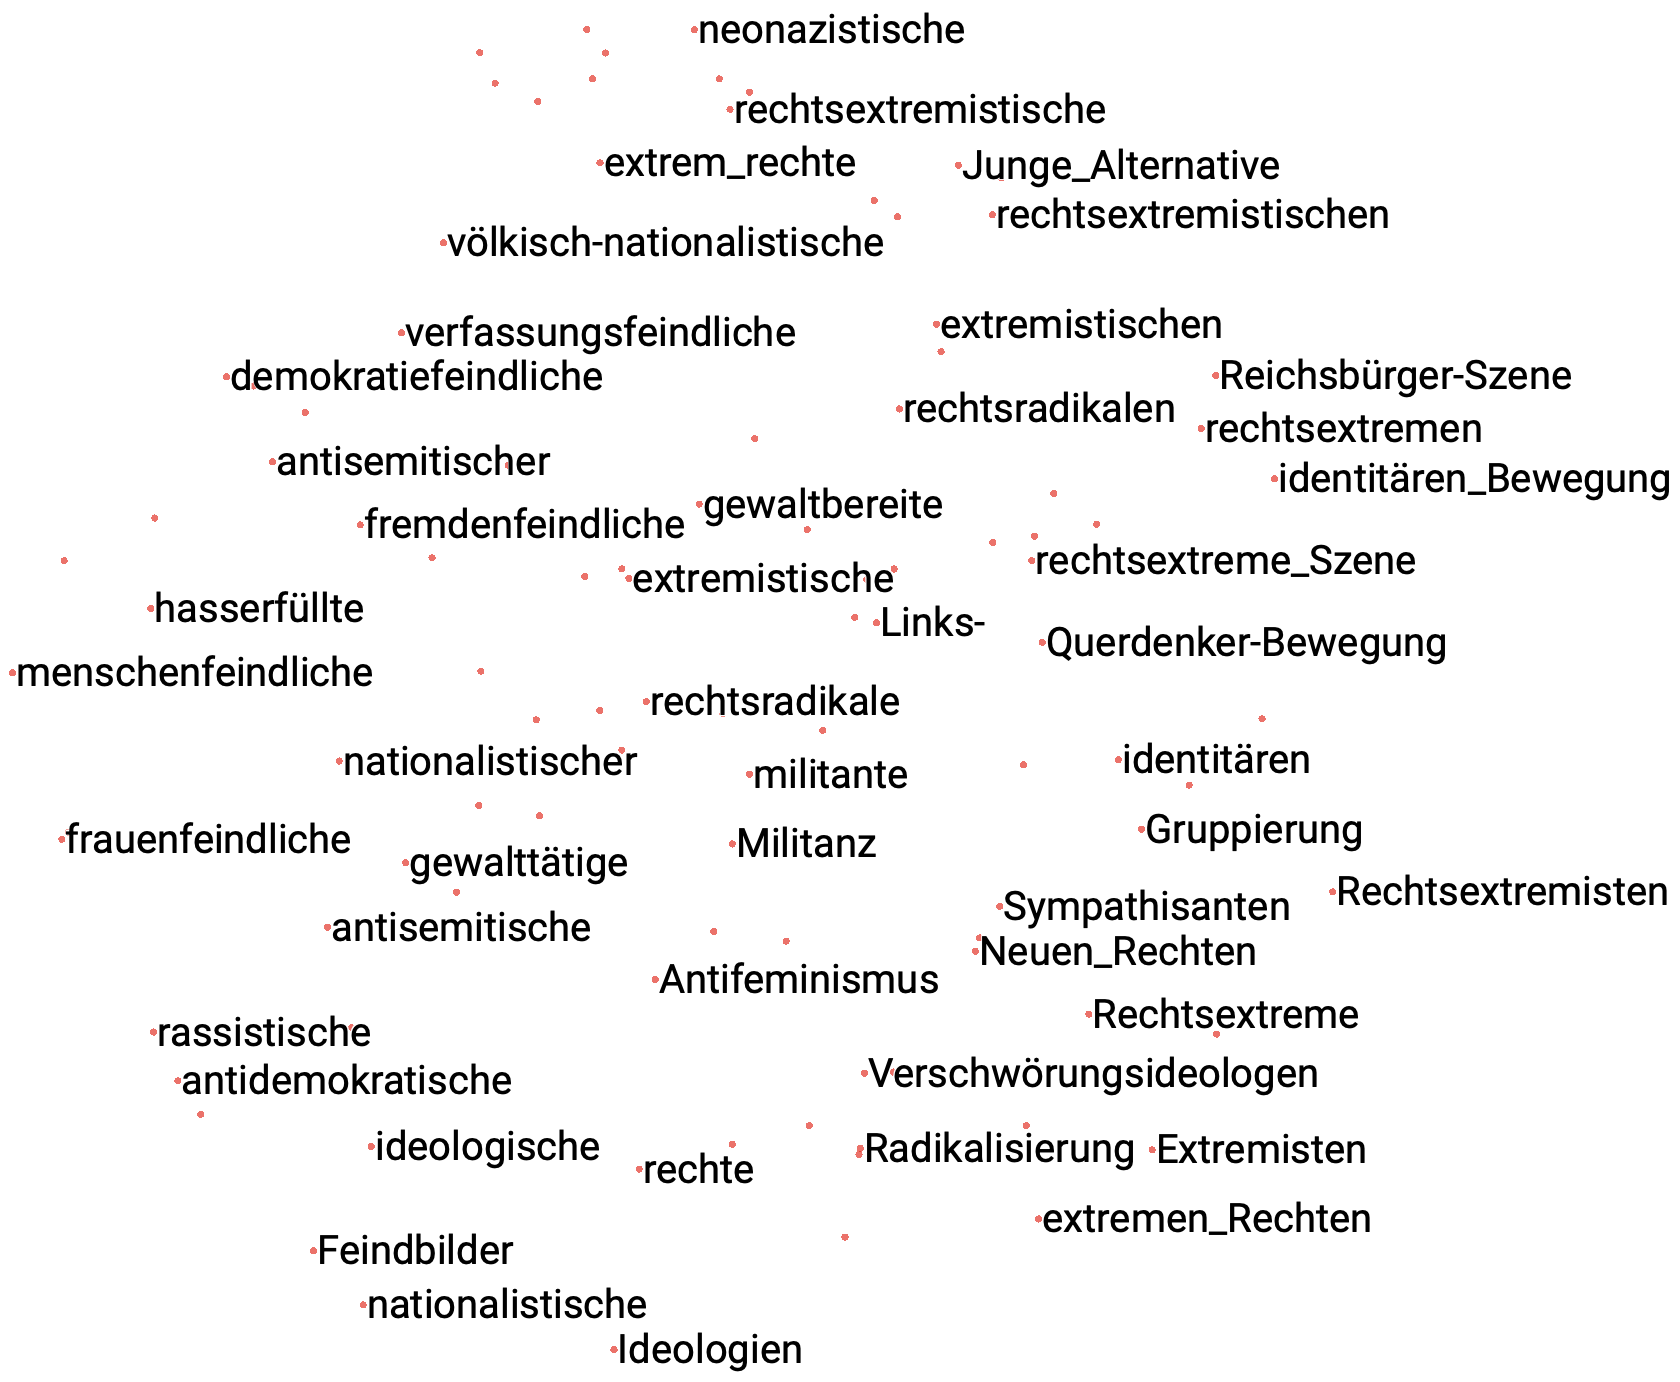
\includegraphics[width=\textwidth]{figures/media/image16.png}
  \caption{\label{fig:pca-nachbarn-extremistische}Nächste paradigmatische Nachbarn zu \emph{extremistische} im Zeitraum 2020--2021 (Dimensionsreduktion mit PCA).}
\end{figure}

Es wird deutlich, dass sich eine Vielzahl semantisch und oft zugleich morphosyntaktisch sehr ähnlicher Wörter im Umfeld des Wortes befinden, wie z.\,B. \emph{neonazistische}, \emph{rechtsradikale} oder \emph{extremistischen}. Andere Ausdrücke erscheinen nicht gleichermaßen bedeutungsähnlich, lassen sich jedoch unschwer als zum Extremismusdiskurs gehörig identifizieren und spielen in diesem etwa als Akteure bzw. Organisationen (u.\,a. \emph{Querdenker-Bewegung}, \emph{Reichsbürger-Szene}, \emph{Neuen\_Rechten}, \emph{Gruppierung}), oder geradezu definitorische Charakteristika (u.\,a. \emph{antidemokratische}, \emph{verfassungsfeindliche}, \emph{ideologische}) eine Rolle. Es deutet sich zudem an, dass es nicht notwendig ist, diese Kategorien im Vorhinein zu definieren und auf die Daten anzuwenden. Vielmehr finden wir sie in der Struktur des Vektorraums bereits wieder und können Cluster erkennen (rechts: Akteure und Organisationen; links: Charakteristika von Extremismus; oben: globalere attributive Bezeichnungen für Extremismus(-formen)). Die Kategorien sind darüber hinaus in diskursanalytischer Literatur bereits als für den Extremismusdiskurs bedeutsam und strategisch veränderlich herausgearbeitet (\chapref{extremismus-in-den-sozialwissenschaften} und \ref{extremismus-diskurs}) und in \chapref{inhaltliche-mindestanforderungen-an-einen-extremismus-frame} als Kandidaten für FE eines Extremismus-Frames ins Auge gefasst worden. Es liegt daher nahe, Cluster von Word Embeddings als FE zu operationalisieren.

Um nicht bei einer visuellen Inspektion einzelner Cluster um ausgewählte Wörter zu verbleiben, ist es sinnvoll, den gesamten Datensatz einem Clustering-Verfahren zu unterziehen. Hierzu wurde der in \chapref{clustering-von-word-embeddings} beschriebene \emph{k-Means}-Algorithmus verwendet, der auch große Datenmengen prozessieren und in eine zuvor festgelegte Anzahl von \emph{k} Clustern gliedern kann. Die Wahl des Parameters ‚\emph{k}` ist dabei natürlich entscheidend und es bestehen unterschiedliche Möglichkeiten, diesen auszuwählen. Mitunter wird von Seiten korpuslinguistischer Diskursanalytiker*innen die Kritik geäußert, dass sich Arbeiten, die solche Verfahren verwenden, zwar einen objektivistischen Anstrich geben wollen, durch die Wahl einzelner Parameter ihre Ergebnisse aber auf eine Art vorformen, die dem \emph{cherry-picking} nahekommt. So formulieren Brookes \& McEnery in Bezug auf die Auswahl von \emph{k} bei Topic Modeling:

\begin{quote}
Total accountability and falsifiability present a way for discourse analysts to avoid the charge of cherry-picking examples to prove a particular argument (Widdowson, 2004). Similarly, topic modelling appears objective and data-driven in as much as the topic discovery procedure is automatic and there seems to be limited scope for the human user to impose any extra-data or pre-analytical categories onto the topics generated. However, as we pointed out earlier in this section, the human researcher is still required to make an important decision about the number of topics generated. This decision is relatively arbitrary. \autocite[7]{brookesUtilityTopicModelling2019}
\end{quote}

Während die Autoren durchaus relevante Probleme am Beispiel der datengeleiteten Generierung von \emph{topics} aufzeigen, die in vielen Beiträgen mehr reflektiert werden müssten, ist ihre Kritik in Bezug auf die Wahl von \emph{k} m.\,E. nicht berechtigt, zumindest wenn die Festlegung gar nicht als ‚objektive` Entscheidung intendiert ist. Vielmehr stellt die Wahl des Parameters eben eine Strukturierungsmöglichkeit der Daten dar, die unterschiedlich fein- oder grobgranulare Ergebnisse zu Tage fördern kann. Ähnlich wie bei einem Mikroskop gilt es also, das methodische Instrument so einzustellen, dass für die jeweilige Forschungsfrage relevante Strukturen sichtbar werden. Dabei kann es auch sinnvoll sein, mit verschiedenen \emph{k} parallel zu arbeiten, wenn es so gelingt, Makro- und Mikrostrukturen herauszuarbeiten und zu kontrastieren. Anstatt den Output eines solchen Verfahrens also als ‚objektiv` anzusehen und zu versuchen, sich der einen ‚richtigen` Variante anzunähern, sollten die Resultate als eine mögliche Strukturierung unter vielen gesehen werden. Auch der Vergleich verschiedener Outputs könnte dann von Interesse sein. Zum Beispiel wäre es denkbar, nachzuverfolgen, welche Wörter bei geringerer Cluster-Größe zusammengefasst und bei höherem \emph{k} voneinander getrennt werden, um lexikalisch-semantische Hierarchien sichtbar zu machen.

In der vorliegenden Arbeit wurde mit unterschiedlichen Cluster-Mengen experimentiert. Beginnend mit einer Einstellung von \emph{k} = 2000, wie sie von Bubenhofer \autocite*{bubenhoferExplorationSemantischerRaeume2022} für Pressedaten verwendet wurde, wurden verschiedene Einstellungen erprobt, wobei sich eine Orientierung an der Korpusgröße bzw. der Anzahl der Vektoren als sinnvoll erwiesen hat. Es erschien also nicht so zu sein, dass das semantische Kategorieninventar von einem Punkt an ausdifferenziert war und zusätzliche Types einfach in diese Kategorien eingeordnet werden. Stattdessen war die Folge einer höheren Type-Anzahl bei gleichbleibendem \emph{k}, dass einzelne Cluster heterogen wurden, also z.\,B. Akteure und ihre Handlungen in den gleichen Clustern zu finden waren. Letztlich wurde entschieden, \emph{k} auf 2,4 \% der Embedding-Anzahl, d.\,h. der Types mit einer Mindestfrequenz von 25 (siehe zu den Type-Anzahlen \chapref{kenndaten-zum-korpus-und-korpusaufbereitung}) einzustellen. So ergaben sich für die diachronen Subkorpora zwischen 2649 (2020--2021) und 4882 (2011--2013) Cluster, für die Zeitungskorpora zwischen 8225 (\textsc{Spiegel}) und 8779 (\textsc{Taz}) Cluster. \tabref{tab:example_clusters} zeigt drei Beispiel-Cluster aus dem Subkorpus 2014--2016, die jeweils nach den drei zentralsten enthaltenen Wortvektoren benannt sind.
\largerpage[-1]
\begin{table}
\caption{Drei Beispiel-Cluster des Zeitraums 2014--2016 und alle enthaltenen Wörter (gereiht nach Nähe zum Cluster-Centroid).}
\label{tab:example_clusters}
 \begin{tabularx}{\textwidth}{>{\hsize=0.5\hsize}X >{\hsize=1.5\hsize}X}
  \lsptoprule
  Cluster & Enthaltene Wörter \\
  \midrule
  \cluster{rechtsradikale{\breakbar}rechtsradikalen{\breakbar}rechtsextreme} & \emph{rechtsradikale, rechtsradikalen, rechtsextreme, rechtspopulistischen, rechtsextremen, rechte, rassistischen, fremdenfeindliche, fremdenfeindlichen, nationalistische, nationalistischen, rechtspopulistische, rechter, antisemitischen, rassistische, antisemitische, rechten, radikalen, radikale, linker, Erstarken} \\
  
  \cluster{Asylbewerber\-unterkunft{\breakbar}Asylunterkunft{\breakbar}Asylbewerberheim} & \emph{Asylbewerberunterkunft, Asylunterkunft, Asylbewerberheim, Gaststätte, Flüchtlingsheim, Lagerhalle, Mehrfamilienhaus, Scheune, Kaserne, Brandstiftung, Synagoge} \\
  
  \cluster{Heidenau{\breakbar}Freital{\breakbar}Bautzen} & \emph{Heidenau, Freital, Bautzen, Clausnitz, Tröglitz, Hoyerswerda} \\
  \lspbottomrule
 \end{tabularx}
\end{table}
Mithilfe des Clusterings gelingt es also, datengeleitet semantische Kategorien, die in der sprachlichen Oberfläche enkodiert und als FE eines Extremismus-Frames lesbar sind, zu erschließen. Hier könnte man die FE als ‚Attribute rechtsextremener Akteure`, ‚Ziele rechter Brandanschläge` und ‚Orte rechtsextremer Anschläge in Ostdeutschland` lesen. Dabei ist die Sichtung der zu einem Cluster gehörigen Wörter und ihre Interpretation als FE ein hermeneutischer Akt. Sein Ziel besteht darin, den größtmöglichen gemeinsamen semantischen Nenner der im Cluster enthaltenen Wörter zu identifizieren. Dabei muss nicht auf das reduktionistische Konzept einer lexikalischen Ausdrucksbedeutung zurückgegriffen werden. Stattdessen können paradigmatische (die anderen Wörter des Clusters) und syntagmatische (kookkurrierende Cluster) Kontextualisierungshinweise einbezogen werden; insbesondere wenn die Interpretation auf Basis des visualisierten Graphen erfolgt. So wird schnell ersichtlich, dass etwa \cluster{14\_Heidenau{\breakbar}Freital{\breakbar}Bautzen} mit anderen Clustern wie u.\,a. \cluster{14\_Notunterkunft{\breakbar}Erstaufnahmeeinrichtung{\breakbar}Unterkunft}, \cluster{14\_Bränden{\breakbar}Unfällen{\breakbar}Zwischenfällen}, \cluster{14\_Ausschreitungen} vorkommt und insofern nicht einfach als ‚Orte` oder ‚Kleinstädte` gelesen werden kann. Es kommt dabei regelmäßig vor, dass sich ein solcher gemeinsamer Nenner für die meisten Wörter finden lässt, jedoch einzelne andere Wörter des Clusters davon mehr oder weniger abweichen. Dies zeigt sich z.\,B. beim Cluster \cluster{14\_rechtsradikale{\breakbar}rechtsradikalen{\breakbar}rechtsextreme}, das auch \emph{linker} und \emph{Erstarken} an seinen Rändern enthält. Auf dieses und andere potenzielle Probleme bei der Auswertung der gewonnenen distributionellen Muster wird in \chapref{wie-der-graph-zu-lesen-ist-und-moegliche-fallstricke} noch vertieft eingegangen.

\subsubsection{Nähe im Vektorraum als Frame-Evokationspotenzial und Perspektivierung}\label{naehe-im-vektorraum-als-frame-evokationspotenzial-und-perspektivierung}

Auf Basis des geclusterten WEM ist es nun möglich, nicht nur die benachbarten Wörter, sondern auch benachbarte Cluster zu Wörtern oder anderen Clustern zu berechnen. Jedes Cluster wird dabei durch den Vektor repräsentiert, der den Mittelpunkt des Clusters, d.\,h. mathematisch das arithmetische Mittel der beinhalteten Vektoren, darstellt. So ist das Embedding \emph{Npd} in der \textsc{Welt} umgeben von den Clustern \cluster{we\_Rechtsextremisten{\breakbar}Neonazis{\breakbar}Rechtsextremen}, \cluster{we\_Linkspartei{\breakbar}Pds{\breakbar}Linken}, \cluster{we\_Gauland{\breakbar}Meuthen{\breakbar}Petry}, \cluster{we\_Verfassungsschutz} und \cluster{we\_rechtsradikalen{\breakbar}rechtsextremistischen{\breakbar}linksextremen}. Es wird deutlich, dass auf diese Weise ein breiter Teil des verstehensrelevanten Wissens zu einzelnen Wörtern zugänglich ist. Frame-semantisch gewendet lassen sich die benachbarten Cluster als FE eines durch das abgefragte Wort evozierten Frames interpretieren, etwa als rechte parlamentarische (\cluster{we\_Gauland{\breakbar}Meuthen{\breakbar}Petry}) und außerparlamentarische (\cluster{we\_Rechtsextremisten{\breakbar}Neonazis{\breakbar}Rechtsextremen}) Akteure, institutionelle Gegenspieler (\cluster{we\_Verfassungsschutz}) oder attributive Zuschreibungen (\cluster{we\_rechtsradikalen{\breakbar}rechtsextremistischen{\breakbar}linksextremen}).

Um die Cluster zu identifizieren, die eine Rolle im Extremismusdiskurs spielen, wurde ein Verfahren entwickelt, das in der Lage ist, anhand einiger weniger \emph{seed words} jedes Cluster in Hinblick auf seine semantische Nähe zum Extremismusdiskurs zu verorten. Die einzelnen ausgewählten \emph{seed words} spielen dabei eine untergeordnete Rolle, da sie nur den Ausgangspunkt für ein Verfahren darstellen, das ein sehr breites lexikalisches Repertoire an thematisch einschlägigen Wörtern und mithin Möglichkeiten des Framings zu Tage fördert. Die Auswahl der \emph{seed words} sollte einerseits auf Basis der FE eines losen provisorischen Frame-Konzeptes, wie es in \chapref{inhaltliche-mindestanforderungen-an-einen-extremismus-frame} skizziert wurde, andererseits auf Basis morphosyntaktischer Kategorien erfolgen, da das Word-Embedding-Modell sowohl auf semantischen als auch auf grammatischen Faktoren beruht. Auf Basis der \emph{seed words}\footnote{Es wurden die folgenden \emph{seed words} verwendet: \emph{Extremismus}, \emph{extremistische}, \emph{extremistisch}, \emph{Radikalismus}, \emph{Rechtsextremismus}, \emph{rechtsextremistische}, \emph{rechtsextremistisch}, \emph{rechtsradikale}, \emph{rechtsradikal}, \emph{Rechtsradikalismus}, \emph{Linksextremismus}, \emph{linksextremistische}, \emph{linksextremistisch}, \emph{linksradikale}, \emph{linksradikal}, \emph{Linksradikalismus}, \emph{Islamismus}, \emph{islamistische}, \emph{islamistisch}, \emph{angreifen}, \emph{begangen}, \emph{verübt}, \emph{Attentat}, \emph{Anschlag}, \emph{Npd}, \emph{Neonazis}, \emph{Antifa}, \emph{islamischer}\cluster{\_}\emph{Staat}, \emph{Bin}\cluster{\_}\emph{Laden}, \emph{Taliban}.}, die einerseits die etablierten Extremismusvarianten ‚Rechtsextremismus`, ‚Linksextremismus` und ‚Islamismus`, andererseits unterschiedliche Flexionsformen und Wortarten abdecken, konnte eine Liste von Clustern berechnet werden, die eine thematische Nähe zum Extremismusdiskurs aufweisen, d.\,h. FE in einem Extremismus-Frame darstellen. Die genauere Funktionsweise des Verfahrens wird in \chapref{berechnung-des-extremismus-centroid-und-begrenzung-der-knotenmenge} dargestellt. Der Mittelpunkt dieser berechneten Cluster, im Folgenden als Extremismus-Centroid bezeichnet, kann nun als Referenzpunkt dienen, um andere Punkte im Vektorraum wie einzelne Word-Embeddings oder Cluster-Centroids hinsichtlich ihrer semantischen Nähe zum Thema Extremismus zu verorten. \tabref{tab:cluster_distances_centroid} zeigt ausschnittsweise die Ergebnisse dieser Analyse für die \textsc{Taz}. Es wird deutlich, dass die Cluster, die dem Extremismus-Centroid relativ nah sind, in der Tat Wörter enthalten, die eindeutig Teil des Extremismusdiskurses sind bzw. einen Extremismus-Frame evozieren (z.\,B. \emph{Extremisten}, \emph{Hisbollah}, \emph{Neonazis}), während die positiv konnotierten Wörter am anderen Ende des Spektrums wie \emph{schwärmt} oder \emph{tolle} keinen Bezug zum Thema Extremismus aufweisen.

\begin{table}[b]
\caption{Beispiele für Cluster mit unterschiedlicher Distanz zum Extremismus-Centroid.}
\label{tab:cluster_distances_centroid}
 \begin{tabularx}{\textwidth}{>{\hsize=0.6\hsize}X >{\hsize=1.4\hsize}X}
  \lsptoprule
  Cosinus-Ähnlichkeit & Cluster \\
  \midrule
  sehr hoch (\textgreater= 0.53) & \cluster{ta\_Extremisten{\breakbar}Islamisten{\breakbar}Dschihadisten} (0.78) \\
                                & \cluster{ta\_Hisbollah{\breakbar}Hamas{\breakbar}Pkk} (0.73) \\
                                & \cluster{ta\_Terrorismus{\breakbar}Terror} (0.65) \\
                                & \cluster{ta\_Rechtsextremisten{\breakbar}Neonazis{\breakbar}Rechtsextremen} (0.53) \\
  \midrule
  eher hoch (\textasciitilde{} 0.27) & \cluster{ta\_Rede} (0.27) \\
                                     & \cluster{ta\_Verbreitung} (0.27) \\
                                     & \cluster{ta\_Unterschrift} (0.27) \\
                                     & \cluster{ta\_Rot-grün{\breakbar}Schwarz-gelb} (0.27) \\
  \midrule
  eher niedrig (\textasciitilde{} 0.14) & \cluster{ta\_Krankenkassen{\breakbar}Kassen} (0.14) \\
                                        & \cluster{ta\_Privatisierung} (0.14) \\
                                        & \cluster{ta\_Plänen} (0.14) \\
                                        & \cluster{ta\_Sachbearbeiterin{\breakbar}Sekretärin{\breakbar}Putzfrau} (0.14) \\
  \midrule
  sehr niedrig (\textless= -0.31) & \cluster{ta\_samt{\breakbar}nebst{\breakbar}inklusive} (-0.31) \\
                                  & \cluster{ta\_bietet} (-0.31) \\
                                  & \cluster{ta\_wunderbare{\breakbar}tolle{\breakbar}schöne} (-0.39) \\
                                  & \cluster{ta\_schwärmt} (-0.39) \\
  \lspbottomrule
 \end{tabularx}
\end{table}
Dass Cluster, die die ausgewählten \emph{seed words} beinhalten, besonders nah am Extremismus-Centroid zu finden sind, liegt in der gewählten Methodik begründet, da sie ja der Ausgangspunkt für dessen Berechnung sind. Unter den 1256 Clustern mit insgesamt 70\,393 Types, die im \textsc{Taz}-Frame einbezogen wurden, enthalten jedoch nur 21 Cluster \emph{seed words}, sodass die Methode es hier durchaus erlaubt, weit über diese hinauszugehen. Dies zeigen auch die Cluster in der Tabelle mit einer eher hohen Cosinus-Ähnlichkeit. Sie können als Teil des politischen Vokabulars durchaus eine Rolle im Extremismusdiskurs spielen, sind aber auch Teil einer Vielzahl anderer thematischer Diskurse. Die Wörter mit einer eher niedrigen Cosinus-Ähnlichkeit wiederum haben zumindest noch entfernt mit dem politisch-institutionellen Bereich zu tun, während die Wörter am unteren Ende der Skala wohl nur sehr selten im Extremismusdiskurs vorkommen. Insgesamt ist bei der Analyse jedoch zu beachten, dass sie eher eine grobe Orientierung bietet und man einzelne Cluster von Hand wahrscheinlich anders ordnen würde. Sie ermöglicht unter Frame-semantischer Perspektive jedoch näherungsweise, das Evokationspotenzial von Wörtern als Spektrum zu modellieren. Dies ist kongruent mit Barsalous und Minskys Annahme eines probabilistischen „matching process`` \autocite*[2]{minskyFrameworkRepresentingKnowledge1974} beim Aufrufen von Frames und geht über \emph{FrameNet} hinaus, wo einzelne LE einem Frame gleichberechtigt zugeordnet sind. Wollte man die Fillmore'sche Trennung von \emph{evocation} und \emph{invocation} aufrechterhalten \autocite[dazu kritisch][]{busseFrameSemantikKompendium2012} und diese zugleich (distributionell\mbox{-}) semantisch statt valenzgrammatisch begründen, könnte man sie anhand der sortierten Cluster-Liste vornehmen, indem man einen Cosinus-Wert als Grenzwert festlegt. Man müsste sich aber im Klaren sein, dass man es dabei mit der notwendigerweise vereinfachenden Einteilung eines Spektrums in zwei Kategorien zu tun hat, nicht mit einem genuin binären linguistischen Phänomen.

Durch die datengeleitete Einteilung des Korpus in Wort-Cluster, die mehr oder weniger Teil des Extremismusdiskurses sind, und ihre Operationalisierung als FE, eröffnet sich zudem eine erste Möglichkeit, Perspektivierung als einen Grundbestandteil Frame-semantischer Theorien (siehe \chapref{perspektivierung-kontext-und-frame-wandel}) abzubilden. Bezieht man nämlich bei der Rekonstruktion des Extremismus-Frames nur die Cluster ein, die eine gewisse Nähe zum Extremismus-Centroid aufweisen, werden kontextfremde Relationen polysemer Cluster ausgeblendet (siehe zur Operationalisierung der FE-Relationen Kapitel \ref{kollokation-von-word-embedding-clustern-als-frame-relationen-und-perspektivierung-kollokationsnetzwerke-als-frames}). Zu einem Cluster wie \cluster{17\_Lastwagen{\breakbar}Lkw} werden also nicht alle syntagmatisch assoziierten FE wie u.\,a. auch \cluster{17\_Fahrzeuge{\breakbar}Autos{\breakbar}Pkw} oder \cluster{17\_beim\_Überholen{\breakbar}am\_Fahrbahnrand{\breakbar}Müllwagen} dargestellt, sondern insbesondere solche, die für den Extremismus-Diskurs thematisch einschlägig sind und es so in Hinblick auf seine Semantik im Extremismusdiskurs bzw. im Kontext des Anschlags vom Berliner Breitscheid-Platz perspektivieren (\cluster{17\_Attentäter}, \cluster{17\_Amri}, \cluster{17\_getötet\_worden{\breakbar}verletzt\_worden{\breakbar}ums\_Leben\_gekommen}).

Betrachtet man noch einmal die in den Word-Embedding-Clustern enthaltenen Wörter (\tabref{tab:example_clusters}) und paradigmatische Cluster-Nachbarschaften (siehe \tabref{tab:collocations_neighbors} im folgenden Kapitel), so wird die paradigmatische Ausrichtung von WEM deutlich. In einem Cluster wie \cluster{14\_Heidenau{\breakbar}Freital{\breakbar}Bautzen} finden sich ausschließlich andere Kleinstädte, jedoch keine Ausdrücke wie \emph{leben}, \emph{ostdeutsch}, \emph{protestieren} oder \emph{Brandanschlag}, die man im syntagmatischen Umfeld erwarten könnte. Um Frame-semantische Relationen zwischen den Clustern beschreiben zu können, wurde daher ihre Distribution auf der syntagmatischen Achse, d.\,h. Kollokationen der Cluster miteinander, berechnet. Das folgende Kapitel wird zeigen, wie sich diese Kollokationen als Frame-Relationen lesen lassen.

\subsubsection{Kollokation von Word-Embedding-Clustern als Frame-Relationen und Perspektivierung, Kollokationsnetzwerke als Frames}\label{kollokation-von-word-embedding-clustern-als-frame-relationen-und-perspektivierung-kollokationsnetzwerke-als-frames}

Die Kollokation, d.\,h. das statistisch signifikante gemeinsame Auftreten von Wörtern \autocite{bubenhoferSprachgebrauchsmusterKorpuslinguistikAls2009}, ist eines der zentralen Konzepte in korpuslinguistischen Ansätzen (siehe \chapref{distributionelle-semantik}, \ref{distributionell-semantische-methodik} und \ref{kollokationen-als-syntagmatische-distributionelle-muster}). Kollokationen beschreiben sprachoberflächliche Distributionen von Korpus-Types (typischerweise Wortformen oder Lemmata) auf der syntagmatischen Achse. Sie machen also die Interaktion von Wörtern sichtbar, jedoch ohne dabei etwas über den Typ der Interaktion auszusagen, also z.\,B. in welchem grammatischen oder semantischen Verhältnis sie stehen. Während die Berechnung von Kollokationen klassischerweise zu den \emph{corpus-based} Methoden zählt, ist die Berechnung ganzer Kollokationsnetze, bei der für jeden Korpus-Type seine Kollokatoren berechnet werden, ein \emph{corpus-driven} Verfahren, das nicht nur auf ausgewählte Wörter angewandt wird (siehe \chapref{begriffsklaerungen-quantitativ-und-qualitativ-corpus-driven-und-corpus-based-sowie-die-rolle-von-hermeneutik}). Hinsichtlich des Ansinnens dieser Arbeit, eine induktive Beschreibung von Extremismus-Frames zu leisten, erscheinen Kollokationsnetze daher geeignet. Ihre Berechnung für ganze Korpora kann jedoch -- je nach Korpusgröße -- sehr rechenintensiv sein und der Output der Analyse aufgrund der Vielzahl der berechneten Kollokationsbeziehungen kaum interpretierbar.\footnote{Für die Subkorpora würden sich Matrizen mit bis zu 365815 x 365815 Werten ergeben (siehe Type-Anzahlen in \tabref{tab:type_frequencies} in \chapref{kenndaten-zum-korpus-und-korpusaufbereitung}).} Für den Einsatz von Kollokationsnetzen ist es also notwendig, die Anzahl der einbezogenen Types mithilfe eines transparenten und begründeten Verfahrens zu reduzieren. So kann man entweder nur lokale Anteile von Kollokationsnetzen um einzelne Wörter betrachten, was wiederum einer verengten \emph{corpus-based} Perspektive entspricht, oder die Type-Anzahl insgesamt reduzieren. Für die Rekonstruktion von Frames, die ich hier in Form eines Kollokationsnetzes anstrebe, sind wesentliche Schritte einer solchen Reduktion durch die im vorigen Kapitel gemachten Ausführungen bereits geleistet. Zum einen werden die Wort-Types des Korpus durch das Clustering auf eine um ein Vielfaches geringere Anzahl von Cluster-Types reduziert. Zum anderen können durch die Berechnung des Evokationspotenzials der einzelnen Cluster solche Cluster aus der Analyse ausgeschlossen werden, die nur mit einer geringen Wahrscheinlichkeit einen Extremismus-Frame evozieren.

\begin{table}\small
\caption{Kollokationen und \emph{next neighbours} im Word-Embedding-Modell zum Cluster \cluster{11\_festgenommen}.}
\label{tab:collocations_neighbors}
 \begin{tabularx}{\textwidth}{lXrXr}
  \lsptoprule
  Rang & Syntagmatisch benachbarte Cluster & Log-Likelihood & Paradigmatisch benachbarte Cluster & Cosinus-Ähnlichkeit \\
  \midrule
  1  & \cluster{11\_wurden}                              & 9420.50   & \cluster{11\_festgenommen\_worden}                     & 0.82 \\
  2  & \cluster{11\_wurde}                               & 8247.68   & \cluster{11\_getötet{\breakbar}erschossen}               & 0.76 \\
  3  & \cluster{11\_Polizei}                             & 4277.99   & \cluster{11\_inhaftiert{\breakbar}hingerichtet{\breakbar}gefoltert} & 0.72 \\
  4  & \cluster{11\_Verdächtigen{\breakbar}Tatverdächtigen{\breakbar}mutmaßlichen\_Täter} & 1983.41 & \cluster{11\_beschuldigt{\breakbar}verdächtigt{\breakbar}angeklagt} & 0.70 \\
  5  & \cluster{11\_Personen}                            & 1749.90   & \cluster{11\_geschnappt{\breakbar}verhört{\breakbar}vernommen} & 0.69 \\
  6  & \cluster{11\_sieben{\breakbar}sechs{\breakbar}fünf}   & 1741.97   & \cluster{11\_ermordet{\breakbar}umgebracht{\breakbar}entführt} & 0.69 \\
  7  & \cluster{11\_Hund{\breakbar}Mann{\breakbar}Tier}      & 1333.86   & \cluster{11\_Entführung{\breakbar}Tötung{\breakbar}Ermordung} & 0.61 \\
  8  & \cluster{11\_31-Jähriger{\breakbar}27-Jähriger{\breakbar}44-Jähriger} & 1130.97 & \cluster{11\_Durchsuchungen{\breakbar}Razzia{\breakbar}Razzien} & 0.59 \\
  9  & \cluster{11\_Demonstranten}                      & 1034.54   & \cluster{11\_angegriffen{\breakbar}attackiert}            & 0.59 \\
  10 & \cluster{11\_festgenommen}                       & 1017.76   & \cluster{11\_Verdächtigen{\breakbar}Tatverdächtigen{\breakbar}mutmaßlichen\_Täter} & 0.58 \\
  \lspbottomrule
 \end{tabularx}
\end{table}
Ich habe also ein Kollokationsnetzwerk für alle Word-Embedding-Cluster berechnet. \tabref{tab:collocations_neighbors} bildet jeweils die Top 10 Kollokate und \emph{next neighbours} im Word-Embedding-Modell zum Cluster \cluster{11\_festgenommen} ab. Im Vergleich zeigt sich deutlich, dass der vektorraumbasierten Rangfolge paradigmatische Ähnlichkeit zugrunde liegt. So finden sich in erster Linie andere Verben in der gleichen Flexionsform (Ränge 1--6 sowie 9) oder verbale Konzepte (Ränge 7--8). Erst auf Rang 10 findet sich ein Cluster, das in einem eher syntagmatischen Zusammenhang zum Ausgangscluster steht, nämlich mögliche Patiens zum Verb \emph{festnehmen}. Als Frame-Relationen gelesen kann eine solche paradigmatische Auswertung also Auskunft über ‚prototypisch assoziierte benachbarte (kontige) Konzepte` \autocite{busseFrameSemantikKompendium2012} geben, nicht jedoch über Frame-Relationen, wie sie etwa in den für die Analyse eines verbalen Konzeptes geeigneten Fillmore-Frames angelegt sind. Ganz anders stellt sich die kollokationsbasierte Rangfolge dar. Hier zeigen sich syntagmatische Beziehungen, die sich als Interaktion der Frame-Elemente lesen lassen. So finden sich sowohl mögliche Besetzungen der Agens- (Rang 3) und Patiens-Rolle (Ränge 4--5, 7--9) als auch zusätzliche Möglichkeiten der semantischen Spezifizierung via Attribuierung (Ränge 6 und 8). Die Benennung der Art der Relation zwischen den Frame-Elementen ist dabei ein rein hermeneutischer und mitunter auf umfangreichem Diskurswissen fußender Akt und nicht unmittelbar aus den quantitativen Daten ablesbar (siehe dazu ausführlicher \chapref{begriffsklaerungen-quantitativ-und-qualitativ-corpus-driven-und-corpus-based-sowie-die-rolle-von-hermeneutik}). Die Kollokationen zeigen also zunächst nur an, dass es einen inhaltlichen Zusammenhang gibt, nicht worin dieser besteht.

Kollokationsnetze bieten neben ihrer induktiven Berechenbarkeit auch den Vorteil, als Netzwerkgraphen visualisierbar zu sein \autocite[siehe ausführlich zu Netzwerkgraphen in der Linguistik][179-192]{bubenhoferVisuelleLinguistikZur2020}. Dabei wurden unter allen Clustern mit einer Mindest-Cosinus-Ähnlichkeit (\textgreater= 0,2 für die diachronen, \textgreater= 0,24 für die Zeitungskorpora) zum Extremismus-Centroid des Zeitraumes jeweils die 20 Cluster mit dem höchsten Kollokationsscore zu diesem Cluster einbezogen. Die Cluster fungieren sodann als Knoten des Graphen, während die Kollokationsscores die Kanten darstellen. Die folgenden Abbildungen zeigen den vollständigen Graphen für die Jahre 2020--2021 (\figref{fig:extremismus-frame-2020-21}), einen Ausschnitt dieses Graphen, in dem Wort-Cluster des Themenfeldes ‚Politik` enthalten sind (\figref{fig:politik-frame-2020-21}), sowie das Cluster \cluster{20\_Hanau} und seine Verbindungen im Graphen (\figref{fig:hanau-frame-2020-21}). Besser explorierbar ist das Netzwerk in der interaktiven Browser-Ansicht; Hinweise zur Bedienung finden sich in \chapref{ueberblick-und-bedienung}. Die erzeugten Visualisierungen sind unter \url{https://doi.org/10.5281/zenodo.10888812} veröffentlicht.

\begin{figure}[t]
  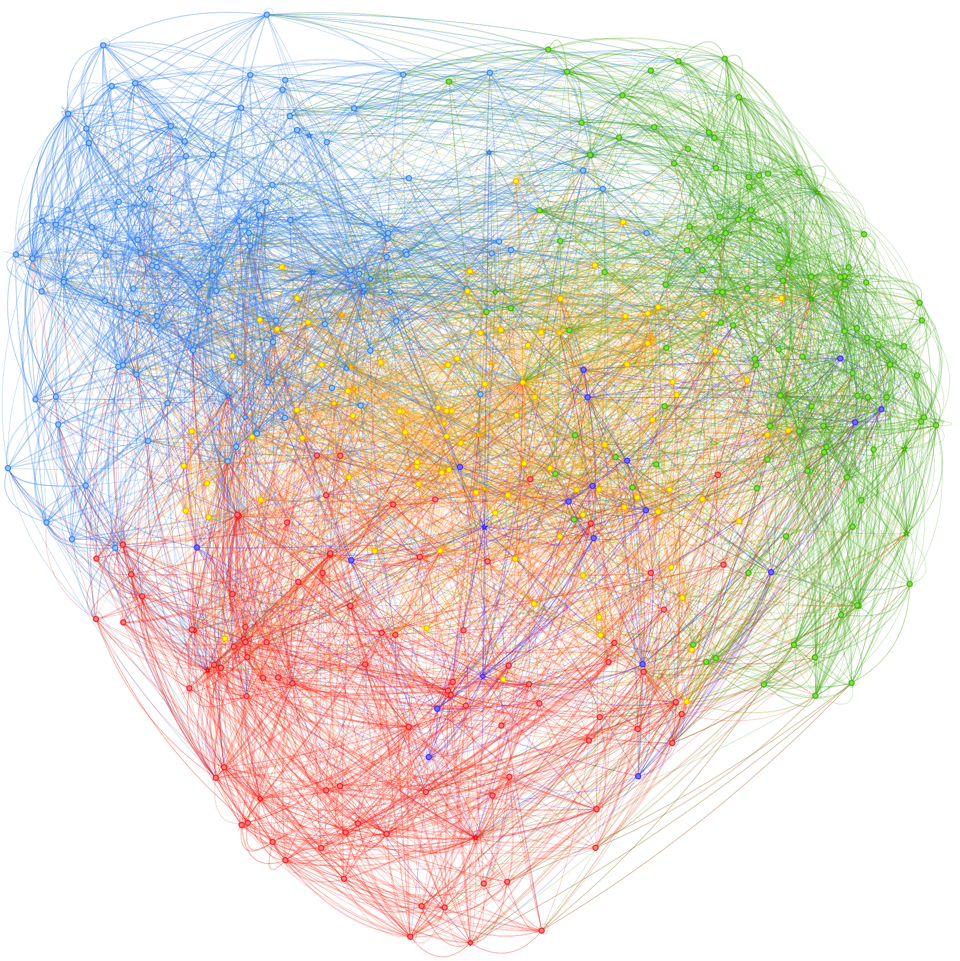
\includegraphics[width=\textwidth]{figures/media/image18.png}
  \caption{\label{fig:extremismus-frame-2020-21}Extremismus-Frame des Zeitraumes 2020--2021.}
\end{figure}

\begin{figure}
  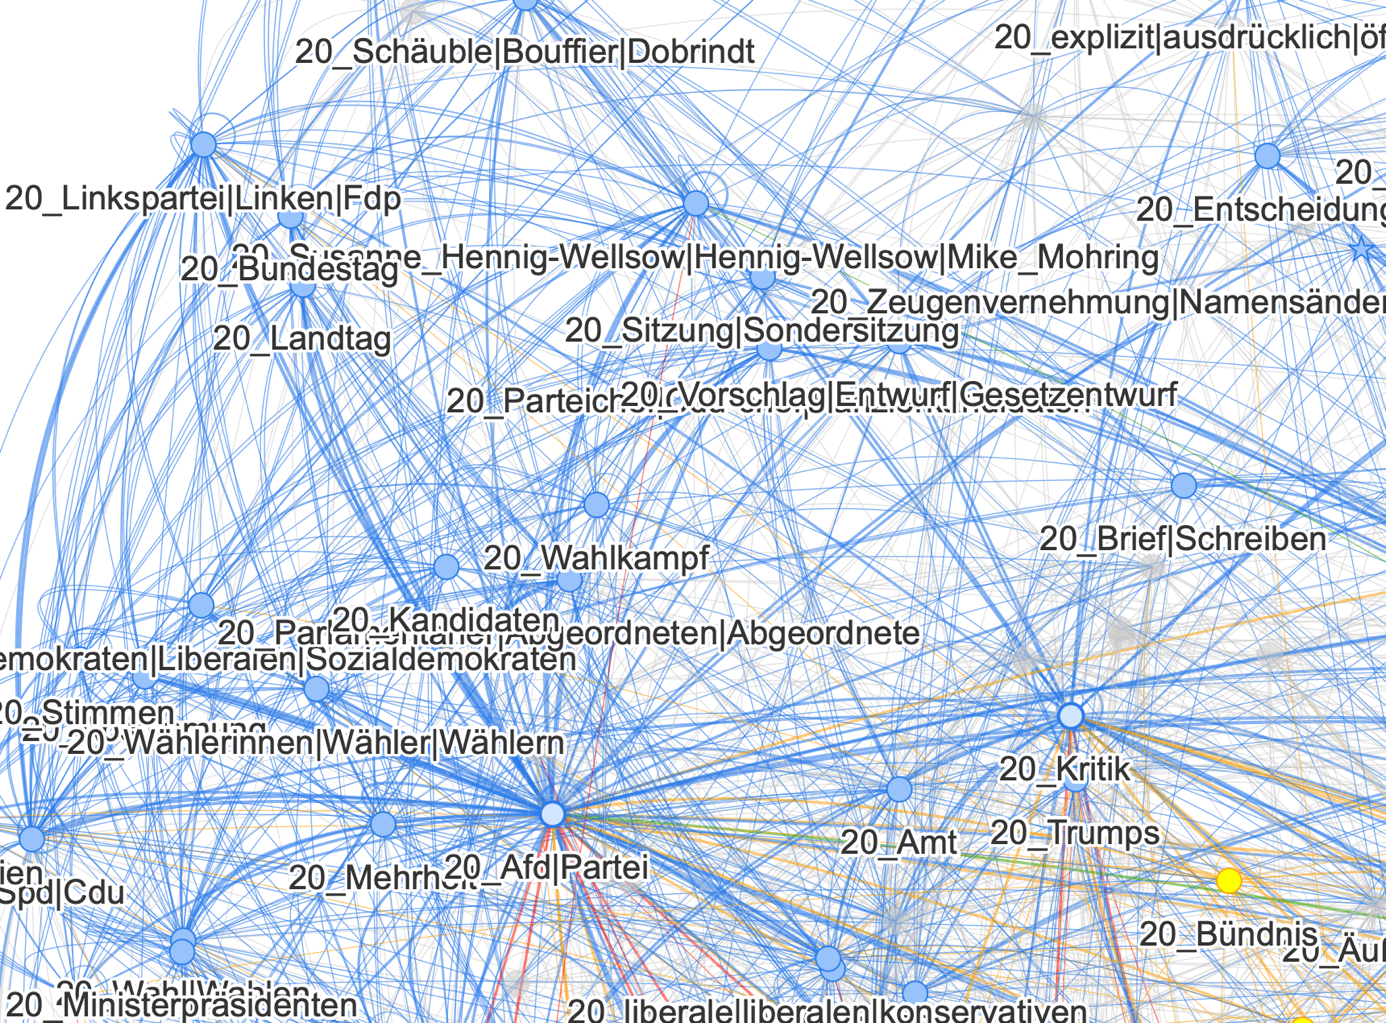
\includegraphics[width=\textwidth]{figures/media/image17.png}
  \caption{\label{fig:politik-frame-2020-21}Ausschnitt aus dem Politik-Teil-Frame des Zeitraums 2020--2021.}
\end{figure}

\begin{figure}
  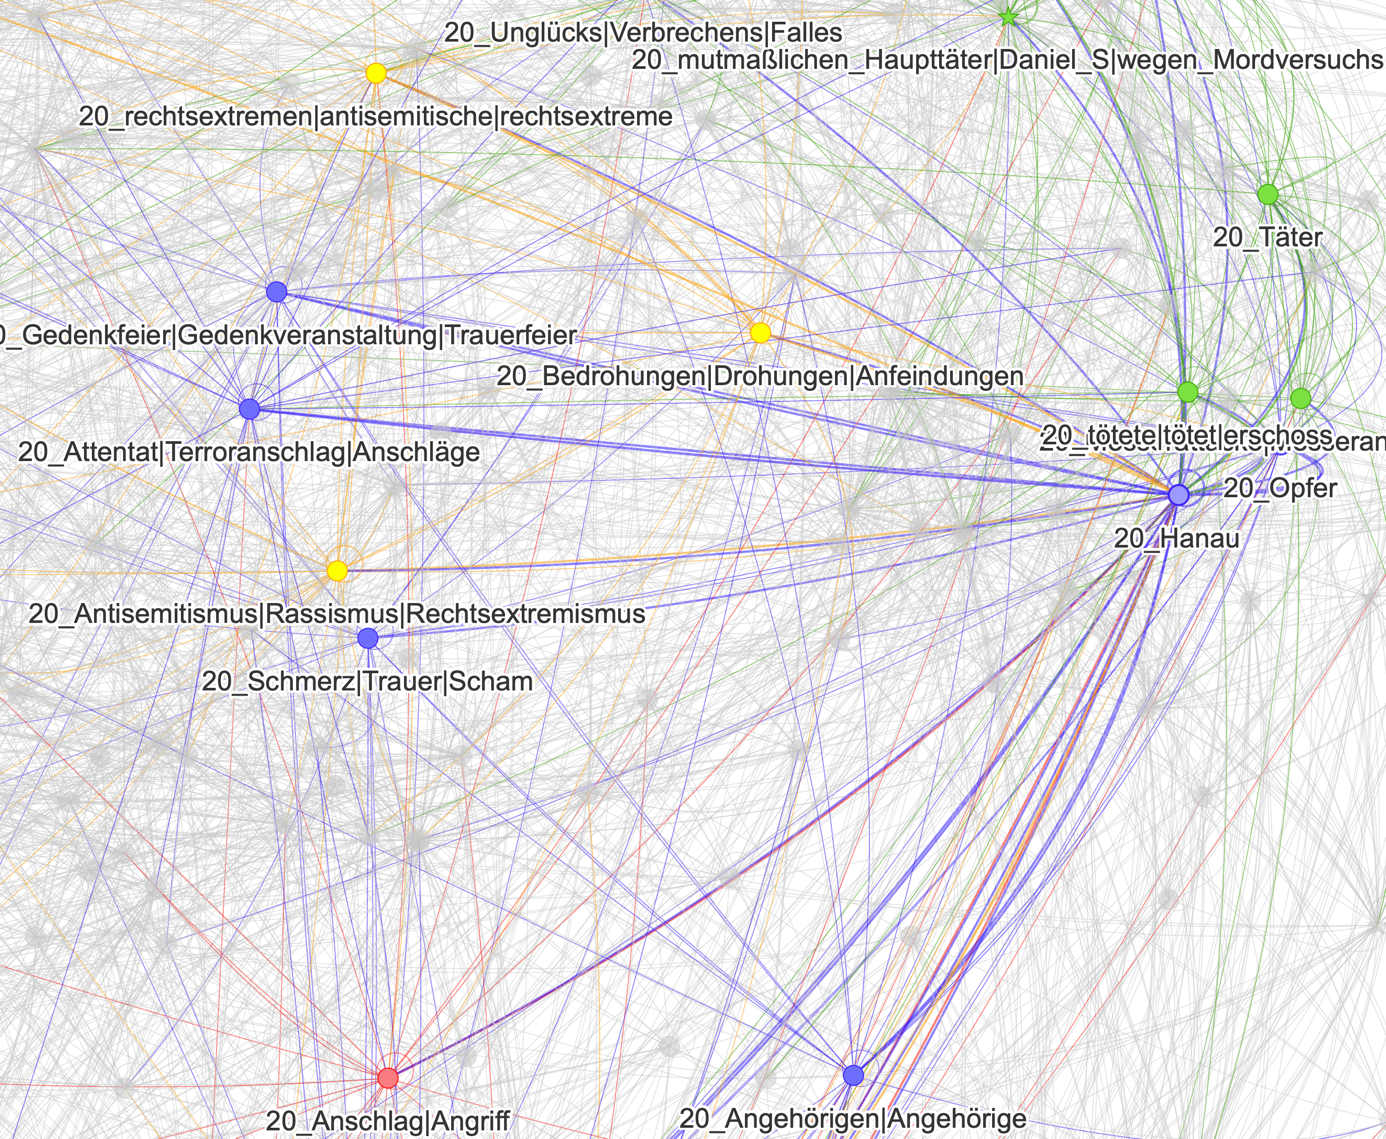
\includegraphics[width=\textwidth]{figures/media/image19.png}
  \caption{\label{fig:hanau-frame-2020-21}Teil des Hanau-Frame des Zeitraums 2020--2021.}
\end{figure}

Das so erstellte Netzwerk kann nun als (Type\mbox{-})Frame gelesen werden, der wesentliche Merkmale von Busse-Frames modelliert. Insbesondere sind dies die Slot-Filler-Struktur, die Rekursivität und unterschiedliche Arten der Frame-Relationen. Die Slot-Filler-Struktur und das Merkmal der Rekursivität sind dabei eng zusammen zu denken: Es lässt sich sowohl das gesamte Netzwerk als ein Frame lesen, der sich aus verschiedenen FE (Slots) zusammensetzt; auch an diese sind jedoch andere FE als Filler angeschlossen, die in Bezug auf wiederum andere FE als Slots agieren. Die Konstituenten der FE, also einzelne zu einem Cluster zusammengefasste Wörter, stellen zugleich die LE dar, die dieses FE evozieren, und darüber hinaus potenzielle Filler eines durch die Liste der LE definierten Wertebereichs. Beispielsweise ist an das Cluster \cluster{20\_Afd{\breakbar}Partei} das Cluster \cluster{20\_Höcke{\breakbar}Kalbitz{\breakbar}Andreas\_Kalbitz} angeschlossen, das im Sinne eines FE ‚Akteure der AfD` interpretierbar ist. Die einzelnen enthaltenen Wörter wie \emph{Kalbitz}, \emph{Flügel} oder \emph{Meuthen} stellen Mögliche Instantiierungen des FE in Token-Frames dar. Dieses FE ist nun selbst wieder ein komplexer Frame und angeschlossene Cluster wie \cluster{20\_Verfassungsschutz}, \cluster{20\_Einstufung} oder \cluster{20\_rechtsradikalen{\breakbar}rechtsradikale{\breakbar}rechtsextremistischen} zeigen an, dass in diesem Zeitraum insbesondere der \emph{Flügel} um \emph{Björn\_Höcke} unter Extremismusverdacht steht bzw. als rechtsextremistisch eingestuft wurde.

Die in den obigen Abbildungen gezeigten Ausschnitte des Graphen sind also jeweils als Frames interpretierbar. Der gesamte Graph in \figref{fig:extremismus-frame-2020-21} ist der Extremismus-Frame für den Zeitraum 2020--2021. Er ist unterteilt in fünf thematische Teil-Frames, die strukturell besonders eng zusammenhängen und farblich markiert sind (siehe \chapref{visualisierung-als-netzwerk-graph-und-erkennung-von-communities}). \figref{fig:hanau-frame-2020-21} stellt die Verbindungen des Clusters \cluster{20\_Hanau} im Graphen dar und lässt sich als Frame zum Anschlag in Hanau im Februar 2020 interpretieren. Während diese drei Struktureinheiten des Netzwerks in einem induktiven Zugang bzw. unter Nutzung etablierter Algorithmen emergent werden, ist es auch möglich, vorwissens- bzw. theoriegeleitete Interessen an den Graphen heranzutragen. So können in einem nächsten Schritt Extremismusvarianten-Frames herausgearbeitet werden. Eine grobe Einteilung kristallisiert sich bereits in der datengeleitet ermittelten Netzwerk-Struktur heraus; Islamismus und politischer Extremismus sind hier stets in unterschiedlichen thematischen Teilen des Netzwerks (Krieg \& Islamismus, Demonstrationen \& Politischer Extremismus) zu finden (siehe zur Analyse der Netzwerk-Communities \chapref{makrostruktur-thematische-teil-frames}). Da sich die Varianten-Frames jedoch auch aus anderen thematischen Bereichen speisen, wurden ergänzend weitere Cluster selektiert, die qua ihrer Kernbedeutung, ihrer Nähe zum Extremismus-Centroid oder aufgrund ergänzender \emph{corpus-driven} Analysen (siehe \chapref{vorgehen-und-zielsetzung}) der jeweiligen Extremismus-Variante zugehörig erscheinen. Idealiter ergeben sich Teile dieser Frames bereits aus den deduktiv ermittelten Strukturen und alle Knoten haben mindestens eine Kante zu einem anderen Knoten des Frames.

\begin{figure}[t]
  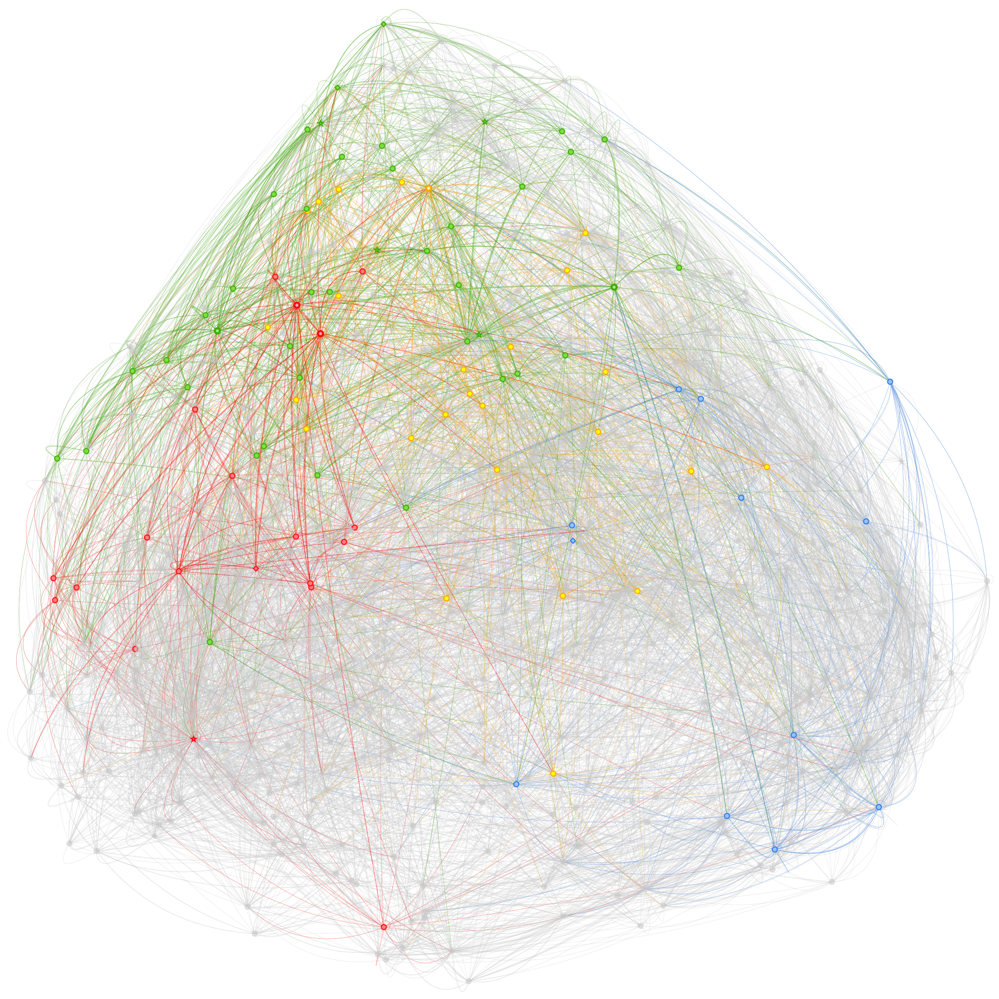
\includegraphics[width=\textwidth]{figures/media/image20.png}
  \caption{\label{fig:rechtsextremismus-frame-1999-2001}Rechtsextremismus-Frame des Zeitraums 1999--2001.}
\end{figure}

~\figref{fig:rechtsextremismus-frame-1999-2001} zeigt die Makrostruktur der Rechtsextremismus-Frames des Zeitraums 1999--2001. Zur Modellierung wurden alle Knoten ausgewählt, die auf Basis von Vorwissen relativ eindeutig der Extremismusvariante zuzuordnen sind (z.\,B. \cluster{99\_Npd}, \cluster{99\_Neonazis{\breakbar}Skinheads{\breakbar}Rechtsextremisten}, siehe \chapref{rechts--und-linksextremismus}). Dieser \emph{corpus-based} Verfahrensschritt ist jedoch eingebettet in die \emph{corpus-driven} ermittelte Struktur, die ergänzend und kontextualisierend wirkt. So werden auch die an die selektierten Knoten angeschlossenen Knoten sowie die Labels der an diese angeschlossenen Knoten angezeigt. Eine Leitlinie besteht außerdem darin, nur solche Knoten auszuwählen, die untereinander vernetzt sind. Dass jeweils ein großer Teil der Knoten zur selben Community gehört, stützt die Hypothese, dass die Extremismusvariante sich auch in der distributionellen Struktur des Korpus niederschlägt. Es finden sich so etwa Praktiken (z.\,B. \cluster{99\_vergewaltigt{\breakbar}überfallen{\breakbar}angegriffen}, \cluster{99\_verletzt\_worden}) und Maßnahmen der Bekämpfung (z.\,B. \cluster{99\_Verbot}, \cluster{99\_verhindern}) als eng assoziiert mit Rechtsextremismus, die nicht vorgegeben waren. Natürlich ist es nicht ausgeschlossen, deduktiv begründete Frames anzunehmen, wenn diese nicht durch die induktiv ermittelte Struktur gedeckt sind. Ausgehend von diesem Ergebnis sollte letztere jedoch noch nicht verworfen werden, sondern geprüft werden, wie der Befund zustande kommen kann -- warum man also einen konzeptuellen Zusammenhang annimmt, der sprachoberflächlich scheinbar nicht realisiert wird. Solche Irritationsmomente können den Blick einerseits auf methodische Defizite lenken, ihn andererseits aber auch für unerwartete Arten der sprachlichen Realisierung von Wissenselementen schärfen und so ein spannender Ausgangspunkt für Folgefragen im Sinne einer ‚quantitativ informierten qualitativen Diskursanalyse` \autocite{bubenhoferQuantitativInformierteQualitative2013} sein.

Die Betrachtung einzelner Knoten des Graphen und ihrer Kanten macht außerdem deutlich, wie einzelne Wörter Frames perspektivieren können. Als Beispiel können die Knoten \cluster{99\_Nazis} und \cluster{99\_Neonazis{\breakbar}Skinheads{\breakbar}Rechtsextremisten} dienen. Beide beinhalten Akteure eines Rechtsextremismus-Frames, die den Frame jedoch jeweils deutlich anders perspektivieren. So ist das Cluster \cluster{99\_Nazis} eng mit dem Bereich des zweiten Weltkriegs bzw. Nationalsozialismus verbunden (u.\,a. \cluster{99\_Holocaust{\breakbar}Nationalsozialismus}, \cluster{99\_Krieg}, \cluster{99\_1945{\breakbar}Zweiten\_Weltkrieg}), während \cluster{99\_Neonazis{\breakbar}Skinheads{\breakbar}Rechtsextremisten} insbesondere in Verbindung mit körperlichen Straftaten und Demonstrationen (u.\,a. \cluster{99\_Demonstranten{\breakbar}Proteste{\breakbar}Protesten}, \cluster{99\_verletzt\_worden}, \cluster{99\_vergewaltigt{\breakbar}überfallen{\breakbar}angegriffen}) vorkommt. Dass sich dies jedoch in einzelnen Vorkommen anders darstellen kann, zeigt Konkordanz K01 in \tabref{tab:K01}.\footnote{Die Konkordanzen werden hier und im Folgenden so wiedergegeben, wie sie im Korpus enthalten sind. Aus diesem Grund ist die Groß- bzw- Kleinschreibung einzelner Wörter verändert und es fehlen Interpunktionszeichen sowie sehr niedrigfrequente Wörter (siehe \chapref{kenndaten-zum-korpus-und-korpusaufbereitung} und \ref{details-der-korpusaufbereitung} zur Korpusaufbereitung).}

\begin{table}
  \caption{Konkordanz zum Ausdruck \emph{Nazis}.}
  \label{tab:K01}
K01 taz\_2208663
\begin{tabularx}{\textwidth}{XcY}
\toprule
man den Rechten keine Plattform geben darf in den Stuben der Verfassungsschutzämter wird lieber geschreddert & \textbf{Nazis} & sind Soziopathen wer sich ihnen offen entgegenstellt braucht Mut und verdient jede Unterstützung ganz am \\
\bottomrule
\end{tabularx}
\end{table}


Man kann diese Äußerung also als Bruch mit dem üblichen Gebrauch des Wortes \emph{Nazis} bzw. der üblichen Versprachlichung zeitgenössischer Akteure des Rechtsextremismus sehen und mithin als Framing rechtsextremer Akteure, in dem auch die historischen Bedeutungsanteile mitschwingen. Aus eher semasiologischer Perspektive zeigen sich Framing-Unterschiede auch an einzelnen Wortformen (siehe auch die Beispiele in \chapref{kenndaten-zum-korpus-und-korpusaufbereitung}). So kommt das Cluster \cluster{20\_Frau{\breakbar}Mann} insbesondere mit Clustern des Bereiches Straftaten \& Juristisches vor (u.\,a. \cluster{20\_belästigt{\breakbar}bedrängt{\breakbar}unter\_Druck\_gesetzt}, \cluster{20\_tötete{\breakbar}erschoss}, \cluster{20\_Polizisten{\breakbar}Beamte}), während \cluster{20\_Frauen{\breakbar}Männer} auch Teil dieses Clusters ist, jedoch ähnlich stark mit dem thematischen Bereich der Gesellschaft \& FdGO assoziiert ist (\cluster{20\_Selbstbestimmung{\breakbar}Gleichheit{\breakbar}Gleichberechtigung}, \cluster{20\_Schutz}, \cluster{20\_Demonstranten}). Assoziierte Cluster wie \cluster{20\_sexualisierte\_Gewalt{\breakbar}sexuelle\_Belästigung{\breakbar}sexuelle\_Gewalt}, \cluster{20\_Bedrohung{\breakbar}Drohungen{\breakbar}Anfeindungen} gehören ebenfalls zu letzterem, liegen jedoch am Übergang der Communities. Es zeigt sich also, dass die vorgeschlagene Methode es ermöglicht, Frames so ausdifferenziert zu beschreiben, dass auch subtile Bedeutungsunterschiede und deren sprachoberflächliche Korrelate sichtbar werden. Dies führt zwar einerseits dazu, dass Frame-Elemente, die man womöglich nicht unterscheiden möchte, in verschiedene Knoten zerfallen (z.\,B. \cluster{99\_Polizei} und \cluster{99\_Polizisten}). Beide Knoten daraufhin bei der Auswertung zum gleichen FE zu zählen, ist jedoch noch immer möglich. Der Vorteil gegenüber einer nicht-datengeleiteten Herangehensweise besteht darin, dass die Unterschiede zunächst für die Forschungsperson sichtbar werden und eine bewusste Entscheidung erfordern, die bestenfalls explizit gemacht und begründet wird -- ein Vorteil des Frame-semantischen Zugangs generell \autocite[341]{busseBedeutungsUndBegriffswissen2018}.

Busse et al. setzen sich ausführlich mit solchen praktischen Problemen der Frame-Darstellung auseinander, wobei sie die Definition der FE als die größte Schwierigkeit ansehen:

\begin{quote}
Das Hauptproblem jeder empirischen Beschreibung von semantischen oder konzeptuellen Frames liegt in der Gewinnung der Slots bzw. Attribute und der jedesmal neu zu treffenden Entscheidung, welche Frame-Elemente angesetzt und in welcher Differenziertheit (hinsichtlich der jeweils anzusetzenden Werte bzw. Filler) sie beschrieben werden sollen. \autocite[77]{busseBedeutungsUndBegriffswissen2018}
\end{quote}

Es gelte, eine schwierige Balance zu wahren zwischen der Überfrachtung des Frames mit zu ausdifferenzierten und letztlich nicht relevanten Frame-Elementen, die sich aufgrund der \emph{Ockhams razor Maxime}\footnote{„Entia non sunt multiplicanda praeter necessitatem``{\slash}„Entitäten dürfen nicht über das Notwendige hinaus vermehrt werden`` \autocite[78]{busseBedeutungsUndBegriffswissen2018}} verbiete, und dem Außer-Acht-Lassen von „banal{[}en{]} und scheinbar selbstverständlich{[}en{]} Wissenselement{[}en{]}`` \autocite[79]{busseBedeutungsUndBegriffswissen2018}, die doch von Relevanz für die Frame-Beschreibung sein könnten. Letztlich schlussfolgern die Autor*innen scheinbar mäßig überzeugt:

\begin{quote}
Im Prinzip muss die Ansetzung jedes einzelnen Elements in Bezug auf die Zielsetzung und das Korpusmaterial streng geprüft und gut begründet werden \autocite[79]{busseBedeutungsUndBegriffswissen2018}.
\end{quote}

Dies ist m.\,E. bei einigermaßen großen Korpora, komplexen sowie wandelbaren Frames und insbesondere aufgrund der Annahme der Rekursivität von Frames ein aussichtsloses Unterfangen. Letztlich konstatieren auch Busse et al. mit Blick auf Barsalou \autocite*{barsalouFlexibilityStructureLinguistic1993}, welcher Arbitrarität und Unvollständigkeit von Beschreibungen rekursiver Frame-Strukturen hervorhebt:

\begin{quote}
so blieb doch auch in unserem Projekt ein Rest an Unsicherheit, ob die angesetzten Frame-Elemente auch wirklich einigermaßen vollständig und ausreichend differenziert beschrieben worden sind. Diese Unsicherheit, die in sprachlichen Dingen (und da hat Barsalou entgegen dem „fröhlichen Positivismus`` der Mainstream-Linguistik durchaus Recht) niemals ganz aus der Welt geschafft werden kann, ist aber nicht mehr oder nicht weniger als die bekannte und unhintergehbare hermeneutische Unvollkommenheit, die in der traditionellen Hermeneutik mit der Metapher des hermeneutischen Zirkels (besser: hermeneutische Spirale) beschrieben worden ist. \autocite[343]{busseBedeutungsUndBegriffswissen2018}
\end{quote}

Die hier vorgeschlagene Methode setzt an, dieses Problem zumindest zu mindern. Sie bietet eine Möglichkeit, eine sehr große Menge rekursiv vernetzter Frame-Elemente auf Basis transparenter Kriterien und einer breiten empirischen Grundlage zu rekonsturieren und in den Frame einzubeziehen. Relevanz für den Frame wird erstens durch semantische Nähe zum Extremismusdiskurs und zweitens durch das überzufällig häufige syntagmatische Ko-Vorkommen von FE bzw. ihrer LE begründet. Beide Parameter sind dabei adjustierbar, um -- in Abhängigkeit vom Untersuchungsinteresse und den forschungspraktischen Möglichkeiten -- eine unterschiedlich große Menge an Frame-Elementen einzubeziehen. Ähnlich formulieren auch Busse et al. in Bezug auf den Auflösungsgrad von Frames:

\begin{quote}
Es sieht ganz so aus, als gebe es für dieses praktische Darstellungsproblem keine allgemeingültige Lösung. Es bleibt wohl nur die Möglichkeit, dies jeweils ad hoc, in Relation zu den jeweiligen Untersuchungszielen und dem gewünschten Auflösungsgrad der Frame-Darstellung zu entscheiden. \autocite[77]{busseBedeutungsUndBegriffswissen2018}
\end{quote}

Die Transparenz, Reproduzierbarkeit und auch Skalierbarkeit eines quantitativen Ansatzes stellen hier jedoch einen entscheidenden Vorteil dar. In Anbetracht der für Frames anzunehmenden Anzahl und Komplexität der enthaltenen Relationen ist es m.\,E. nicht vorstellbar, diese Entscheidungen händisch zu treffen, ohne implizit starke Vereinfachungen des Frames vorzunehmen. Eine kontrastive Untersuchung von Frames in unterschiedlichen diachronen oder medialen Kontexten würde es zudem erfordern, diese Entscheidungen auf eine unvoreingenommene Weise erneut für jeden Kontext zu treffen. Dies würde jedoch jeweils enorme analytische Vorarbeiten erfordern, möchte man die Ausdifferenzierung des Frames gegenstandsadäquat vornehmen und nicht voraussetzen.

\subsubsection{Netzwerk-Communities als thematische Teil-Frames}\label{netzwerk-communities-als-thematische-teil-frames}

Schon bei einer ersten Inaugenscheinnahme der erstellten Netzwerke zeigt sich, dass die Knoten des Graphen nicht gleichmäßig verteilt sind, sondern Cluster bilden. Solche Cluster werden in der Analyse von Netzwerken auch als Communities bezeichnet. Diese Netzwerk-Cluster sind untereinander stärker vernetzt als mit den anderen Communities, was korpuslinguistisch auf dem gemeinsamen Vorkommen der in den beteiligten Word-Embedding-Clustern enthaltenen Wörtern in den Texten des Korpus beruht. Inhaltlich teilen die Netzwerk-Cluster eine semantische Ähnlichkeit und lassen sich den Themen ‚Politik` (in manchen Teilkorpora getrennt nach Innen- und Außenpolitik), ‚Staat, FdGO \& Gesellschaft`, ‚Krieg \& Islamismus`, ‚Straftaten \& Juristisches` sowie ‚Demonstrationen \& Politischer Extremismus` zuordnen (siehe \chapref{makrostruktur-thematische-teil-frames}). Durch die Frame-Modellierung als Graph steht eine Vielzahl an Algorithmen zur Verfügung, die in der Lage sind, Communities datengleitet zu erkennen. Mit ihrer Hilfe können zum einen die mit bloßem Auge sichtbaren Cluster, zum anderen auch weitere Cluster, die aufgrund der vielen, sich zum Teil überlagernden Strukturen sonst unsichtbar geblieben wären, identifiziert werden.\footnote{In der Analyse wurde zu diesem Zeck der \emph{Spin-Glass}-Algorithmus \autocite{reichardtStatisticalMechanicsCommunity2006} verwendet.} Der besonders starke Zusammenhang dieser Netzwerk-Cluster beruht u.\,a. darauf, dass thematische Netzwerk-Cluster, wie ‚Innen- und Außenpolitik` oder ‚Krieg \& Islamismus`, nicht nur innerhalb des Extremismusdiskurses bestehen, sondern in verschiedenen Diskursen wesentliche Anteile thematischer Frames ausmachen bzw. die Themen selbst Diskurse darstellen. Ihre Kollokationsscores sind also besonders hoch im Gegensatz zu Clustern, die jeweils im ganzen Korpus vorkommen, jedoch nur im Kontext Extremismus signifikant häufig gemeinsam. Dies erscheint auch aus gebrauchssemantischer Perspektive plausibel, denn es ist m.\,E. sinnvoll, nicht davon auszugehen, dass Wörter völlig neue Bedeutungen in einzelnen Diskursen annehmen, sondern immer auch Gebrauchsspuren aus anderen Kontexten aufweisen. Auch Frame-semantisch ist der Gedanke solcher thematischen Teil-Frames, die das Extremismuskonzept aus jeweils unterschiedlichen thematischen Perspektiven beleuchten, plausibel. So stellt auch Busse die Rolle von Frame-Systemen heraus:

\begin{quote}
Bereits Fillmore wies vergleichsweise früh darauf hin, dass zum Lexem-bezogenen Wissen nicht nur die Aktivierung eines einzelnen Frames / Schemas gehört, sondern das Wissen darüber, mit welchen Schemata (Szenen, Frames) das Wort / Lexem selbst (oder die durch es aktivierten Frames) zusammenhängt. Er nannte als Beispiel Wortfeld-ähnliche Strukturen, auch wenn er die eigentliche Wortfeldtheorie als unzureichend ansieht. {[}\ldots{]} Minsky erweiterte diesen Aspekt der Perspektive auf die Perspektive im ganz wörtlichen Sinne bei visueller Wahrnehmung, und beschrieb die verschiedenen, vom kognitiven Apparat eines Individuums je getrennt verarbeiteten und konstituierten Perspektiven-Frames auf einen visuell wahrgenommenen Gegenstand (z.\,B. einen Tisch, bei dem ein Bein völlig, bis zu zwei weitere Beine teilweise verdeckt sind) als Elemente eines „Frame-Systems`` {[}\ldots{]}. Solche „Frame-Systeme`` gibt es jedoch nicht nur für verschiedene visuelle Perspektiven (wie bei Minsky), sondern als epistemische Strukturen generell. Fillmores Perspektiven-Frames auf Handlungskomplexe bzw. Ereignisse sind ein Beispiel dafür. Frame-Systeme als Kombinationen von mehreren Perspektiven bzw. Teilaspekte sind daher ein generelleres Phänomen des Wissens und seiner Strukturen. \autocite[635-636]{busseFrameSemantikKompendium2012}
\end{quote}

\largerpage
Die Berechnung der Communities ermöglicht es, den komplexen Extremismus-Frame zunächst makrostrukturell zu gliedern und dabei datengeleitet Themen zu identifizieren, nach denen sich die FE ordnen lassen. Kontrastiv ist es sodann möglich, sowohl Kontinuitäten als auch Umstrukturierungen der Extremismus-Semantik aufzuzeigen. So sind die Cluster ‚(Innen\mbox{-})Politik`, ‚Außenpolitik`, ‚Straftaten \& Juristisches`, ‚Krieg \& Islamismus`, ‚Demonstrationen \& politischer Extremismus` sowie ‚Staat, FdGO \& Gesellschaft` in fast jedem berechneten Frame zu finden, während sich Cluster wie ‚Flucht \& Migration` oder ‚Geheimdienste` nur in manchen Jahren bzw. Zeitungen manifestieren. Besonders interessant ist es, zu betrachten, wie sich einzelne FE zu diesen Clustern verorten und ihre Position in Abhängigkeit der betrachteten Variablen ‚Zeit` und ‚Medium` verändern. Zum Beispiel ist das Cluster \cluster{99\_Npd}, das einem NPD-Frame als Teil des rekursiven Extremismus-Frames entspricht, noch eng mit dem thematischen Bereich ‚Straftaten \& Juristisches` assoziiert und macht so verfassungsrechtliche Mittel der Extremismusbekämpfung in Form eines Parteivervots zum Teil des Framings von Rechtsextremismus. Diese Assoziation verschwindet in den Folgejahren jedoch beinahe vollständig und es bleibt bis zum zweiten NPD-Verbotsverfahren lediglich die Assoziation mit dem Bereich des Politischen und der Demonstrationen (siehe z.\,B. 2008--2010). Die Berechnung und Auswertung der Netzwerk-Cluster ist ein Analyseschritt, der zunächst nicht im Forschungsdesign angelegt war, sondern sich erst beim explorativen Umgang mit den Korpusdaten und der Kombination verschiedener etablierter Verfahren sowie insbesondere der Visualisierung der Ergebnisse dieser Methoden als sinnvoll erwiesen hat.

\subsubsection{Berechnung von Frames auf Basis unterschiedlicher Subkorpora als Modellierung von Kontexten und Frame-Wandel}\label{berechnung-von-frames-auf-basis-unterschiedlicher-subkorpora-als-modellierung-von-kontexten-und-frame-wandel}

Frame-Wandel ist gerade bei abstrakten konzeptuellen Frames die Regel und ein Grundprinzip in Busses Frame-Semantik (siehe \chapref{perspektivierung-kontext-und-frame-wandel}). Wie bereits angedeutet, lassen sich Frames mit dem hier vorgeschlagenen Verfahren für beliebige Teile des Korpus berechnen, eine gewisse Korpusgröße vorausgesetzt. Die Unterteilung in Subkorpora dient dabei in einem korpuspragmatischen Zugang der Modellierung von Kontexten bzw., wenn es um diachrone Gliederungen geht, der Modellierung von Sprach- bzw. Frame-Wandel. Dabei werden einzelne Verfahren auf das gesamte Korpus, andere nur auf die gebildeten Subkorpora (hier: die diachrone Gliederung in Dreijahresabschnitte und die Unterteilung nach Zeitung) angewendet. Für das gesamte Korpus wird zunächst das Phrasing vorgenommen, das signifikante Bi- und Trigramme erkennt und zu je einem Type zusammenführt. Außerdem wird mithilfe von TWEC ein Word-Embedding-Modell, der sogenannte Kompass, auf dem gesamten Korpus berechnet, der im Anschluss dafür genutzt wird, die Modelle der Subkorpora im gleichen Vektorraum zu berechnen.

\largerpage[-1]
Alle weiteren Verfahrensschritte beziehen sich auf die einzelnen Subkorpora: Zunächst wird ein TWEC-Modell für das Subkorpus berechnet und im Anschluss geclustert, wobei es sich bewährt hat, die Cluster-Anzahl \emph{k} nach der Anzahl der Types im Subkorpus zu richten. Wie bereits beschrieben, erfolgt im Anschluss die Berechnung der Kollokationsmatrix und des Netzwerk-Graphen. Der Vergleich der für die einzelnen Teilkorpora erstellten Netzwerk-Graphen zeigt dann Veränderungen und Konstanzen im Sprechen über Extremismus, die sich als Frame-Wandel lesen lassen.

\subsection{Technisch-methodische Umsetzung: Vom rohen Text zum Graphen}\label{technisch-methodische-umsetzung-vom-rohen-text-zum-graphen}

Nachdem das vorige Kapitel die inhaltliche Logik des vorgeschlagenen Verfahrens theoriebezogen dargestellt hat, sollen im Folgenden die technischen Aspekte des Vorgehens beleuchtet werden. Dazu zählen insbesondere die angewandten algorithmischen Schritte bei der Verarbeitung der Texte sowie die Einstellung der jeweiligen Parameter.

\subsubsection{Generelles Vorgehen}\label{generelles-vorgehen}

Sowohl Algorithmen- als auch Parameterwahl haben einen unmittelbaren Einfluss auf die Art und Qualität der Ergebnisse. Bei der Erprobung und Evaluation quantitativer algorithmischer Methoden, insbesondere in der Computerlinguistik, besteht das übliche Vorgehen darin, zunächst einen Goldstandard in Hinblick auf das algorithmisch zu lösende Problem zu etablieren, um daraufhin die Resultate mit diesem zu vergleichen. In der Regel werden dabei manuell vorgenommene Annotationen bzw. \emph{human ratings} zur Grundlage des Goldstandards gemacht oder etablierte \emph{tasks}, für die Lösungen bereitstehen, verwendet. Es werden sodann quantitative Kennwerte berechnet, die eine nachvollziehbare Einschätzung der Qualität der Ergebnisse erlauben. Als Beispiel kann das in \chapref{frame-induktion} berichtete Verfahren zur Frame-Induktion von Yamada et al. \autocite*{yamadaSemanticFrameInduction2021} dienen. Sie entwickeln einen Algorithmus zur Frame-Induktion, dessen Erfolg sie an der Übereinstimmung mit \emph{FrameNet}s „human-annotated frames`` \autocite*[814]{yamadaSemanticFrameInduction2021}, die sie als Goldstandard voraussetzen, messen. Dieses Vorgehen ist mit einem \emph{corpus-driven} Zugang jedoch schwer zu vereinbaren. Wenn in der vorliegenden Arbeit Wissensstrukturen und -elemente datengeleitet durch musterhafte Formationen in der \emph{Parole} rekonstruiert werden, soll dies ja gerade ohne die vorläufige Annahme, Beschreibung und Operationalisierung ebendieser Strukturen und Elemente geschehen.\footnote{Bubenhofer \autocite*{bubenhoferWennLinguistikKorpuslinguistik2018} hebt des Weiteren hervor, dass über den Vergleich mit einem Goldstandard die linguistische Reflektion, warum der Goldstandard erreicht (oder nicht erreicht) wird, oft ausbleibt.} Vielmehr gilt es, eine linguistisch informierte Methodenauswahl zu treffen, mit deren Hilfe Sprachgebrauchsmuster sichtbar und als epistemische Einheiten lesbar gemacht werden können. Natürlich sind dabei auch grobe inhaltliche Vorannahmen unerlässlich, wenn themenbezogen gearbeitet werden soll, denn ohne eine inhaltliche Rahmung und grobe Strukturierung des Forschungsgegenstandes, wie hier in \chapref{extremismus-diskurs} bzw. \ref{inhaltliche-mindestanforderungen-an-einen-extremismus-frame} vorgenommen, können die sprachoberflächlichen Formationen nicht als thematisch einschlägig erkannt werden. Statt ein deduktives, schablonenhaftes Kategoriensystem zu erstellen, in das empirische Daten eingeordnet werden, geht es also darum, Eckpunkte zur Orientierung zu gewinnen. Sprachgebrauchsmuster können so in Bezug zur Theorie gesetzt werden, was es insbesondere ermöglicht, die Art der vorgefundenen sprachlichen Muster und ihre Interpretierbarkeit im Rahmen des Forschungsinteresses einzuordnen. Erst so war es im Rahmen dieser Arbeit möglich, das Potenzial von Word-Embedding-Clustern als Frame-Elemente zu erkennen und die berechnete Anzahl an Clustern so anzupassen, dass der Auflösungsgrad der Frame-Elemente sinnvollen Kategorien des Extremismusdiskurses entspricht.

Der \emph{sweet spot} im \emph{corpus-driven} Ansatz liegt dort, wo die gewählte Methode einerseits vor dem Hintergrund des eingebrachten Diskurswissens wiedererkennbare Sprachgebrauchsmuster zu Tage fördert -- hier etwa als FE operationalisierbare Word-Embedding-Cluster mit Akteuren des Rechtsextremismus (z.\,B. \cluster{17\_Rechtsextremisten{\breakbar}Rechtsextreme{\breakbar}Neonazis}) oder mit ihnen assoziierte Praktiken (z.\,B. \cluster{17\_Demonstration{\breakbar}Kundgebung{\breakbar}Demo}). Auf der anderen Seite werden an diesem \emph{sweet spot} auch eine Vielzahl gleichartiger, d.\,h. auf dieselbe Art lesbarer, Sprachgebrauchsmuster emergent, die nicht bereits intuitiv antizipiert wurden (auffällig ist etwa, dass keine Kante zum Cluster \cluster{17\_Ausschreitungen{\breakbar}Krawallen{\breakbar}Krawalle} besteht) oder in ihrer Menge nicht händisch zu erschließen wären (dies betrifft sowohl die Anzahl der FE als auch insbesondere ihre präzisen sprachlichen Realisierungen in Form einzelner Lexeme oder gar Wortformen). Natürlich fördern datengeleitete Zugänge so auch Ergebnisse zu Tage, die „auf der Hand liegen`` \autocite[430]{roemerBackRootsVerteidigungsrede2022}. Abgesehen davon, dass dies auch für ein Funktionieren des Verfahrens und eine intersubjektive Nachvollziehbarkeit der Ergebnisse spricht, ist m.\,E. doch zu bezweifeln, dass die gleichen Ergebnisse auch in qualitativen Analysen zu gewinnen wären. Als Beispiel mag der in den Kapiteln \ref{kollokation-von-word-embedding-clustern-als-frame-relationen-und-perspektivierung-kollokationsnetzwerke-als-frames} und \ref{rechts--und-linksextremismus} angeführte Befund dienen, dass der Ausdruck \emph{Nazis} eine historische Perspektive auf die Zeit des Nationalsozialismus eröffnet, während Ausdrücke wie \emph{Rechtsextremisten}, \emph{Skinheads} oder \emph{Neonazis} sich vor allem auf zeitgenössische Akteure bzw. Formen des Rechtsextremismus beziehen. In einzelnen Fällen fanden sich aber durchaus auch Gegenbeispiele (siehe Beleg K01 in \tabref{tab:K01}). Natürlich erscheint es zunächst möglich, dies intuitiv zu antizipieren -- fraglich ist m.\,E. aber doch, ob auch graduelle Unterschiede dem qualitativen Blick ohne Weiteres zugänglich sind. Kann man etwa sagen, ob sich diese Verhältnisse im Zeitraum 1999--2001 anders darstellen als in den Jahren 2008--2010? Ob es womöglich generell eine Tendenz gibt, den Ausdruck \emph{Nazis} zunehmend in Bezug auf zeitgenössische Phänomene zu verwenden? Oder ob die \textsc{Welt} mehr dazu neigt als der \textsc{Spiegel}? Solche Differenzen können durchaus eine Rolle spielen, wenn linguistisch-epistemologische Fragen im Detail betrachtet werden, und erschließen sich insbesondere in einem korpuspragmatischen Zugang.

\subsubsection{Details der Korpusaufbereitung}\label{details-der-korpusaufbereitung}

Im Folgenden soll ein Überblick über das im Rahmen dieser Dissertation entwickelte und angewandte Verfahren gegeben werden, wobei die Reihenfolge der Darstellung der Reihenfolge der Anwendungsschritte im Verfahren entspricht. Ausgangspunkt für dieses Kapitel ist die bereits fertig erhobene Textsammlung, die als csv-Datei vorliegt. Hier werden den noch ‚rohen`, d.\,h. linguistisch nicht weiter bearbeiteten Texten eine Reihe von Metadaten wie das Publikationsdatum und die URL zugeordnet. Die Erhebung des Korpus erfolgte mit einem Python-Webscraper, dessen Implementierung sich an den Empfehlungen in Feiks \autocite*{feiksEmpirischeSozialforschungMit2019} orientierte. Es wurde des Weiteren, wie bereits in \chapref{kenndaten-zum-korpus-und-korpusaufbereitung} beschrieben, ein Sample aus den Daten gezogen, das allen weiteren Schritten zugrunde liegt.

Zunächst wurden routinemäßige Schritte der Korpusaufbereitung mit dem \emph{TreeTagger} \autocite{schmidProbabilisticPartSpeechTagging1994} vorgenommen, d.\,h. eine Tokenisierung, Lemmatisierung und ein POS-Tagging. Bei computerlinguistisch geprägten Verfahren sind darüber hinaus weitere Schritte des \emph{preprocessing} verbreitet und für manche Verfahren empfohlen. Diese können z.\,B. eine Kleinschreibung aller Wörter (\emph{lower casing}), das Filtern von \emph{stop words} (je nach Definition sehr häufige Wörter oder Synsemantika) oder das Entfernen von Satzzeichen und Zahlen umfassen \autocite{schumacherPreprocessingMitNLTK2022}. Während wohl kaum eine Korpusuntersuchung ohne Tokenisierung auskommt,\footnote{In Sprachmodellen der neueren Generation wie z.\,B. BERT entsprechen Token aber nicht mehr unbedingt ganzen Wörtern.} sind Schritte wie ein \emph{lower casing} insbesondere für deutsche Sprachdaten nicht unbedingt sinnvoll, da sie in der Sprache bestehende formale Differenzierungen, die auch zur semantischen Disambiguierung beitragen, nivelliert. So gibt es mit der Großschreibung von Nomen-- im Gegensatz zur Großschreibung am Satzanfang -- eine orthographische Differenzierung, die zugleich häufig eine semantische Disambiguierung ermöglicht (z.\,B. \emph{rennen} und \emph{Rennen}). Als Kompromiss zwischen dem Ziel, möglichst viele Informationen aus der sprachlichen Oberfläche zu erhalten und zugleich möglichst viele Belege für einzelne Types beim Training der Word Embeddings berücksichtigen zu können, wurde kein generelles \emph{lower casing} durchgeführt. Stattdessen wurde die Großschreibung der laufenden Wörter nach dem Lemma ausgerichtet, um Großschreibung zu tilgen, die nur auf die Position des Wortes am Satzanfang zurückgeht. So konnte vermieden werden, unterschiedliche Types (und mithin im späteren Verfahren Word Embeddings) für z.\,B. \emph{machen} und \emph{Machen} zu erhalten.\footnote{Eine weitere Möglichkeit zur Disambiguierung stellt der Einbezug der POS-Tags bei der Berechnung von Word-Embeddings dar. Erweitert man jedoch jedes Token um seinen POS-Tag hat dies einen deutlich höheren Arbeitsspeicherbedarf beim Training der Vektoren zur Folge.} Da dieser Verarbeitungsschritt nicht durchweg treffsicher funktionierte, ergaben sich auch orthographisch falsche Schreibweisen wie z.\,B. \emph{Npd}, \emph{Un-blauhelme} oder \emph{Us-regierung}.

Da Zahlen zwar insgesamt häufig im Korpus vorkommen, individuelle Zahlen jedoch zum Teil sehr selten, kann es sinnvoll sein, diese aus dem Korpus zu tilgen oder grundsätzlich zu maskieren, d.\,h. durch ihr POS-Tag (CARD) zu ersetzen. Da jedoch insbesondere Jahreszahlen als potenziell interessant erschienen, wurde entschieden, Zahlen im Korpus zu belassen und in Abhängigkeit ihrer Größe zu maskieren. Zusammengefasst wurden die Zahlen \textless{} 0 als \emph{lt0} (\emph{less than} 0), \textless{} 10 als \emph{lt10}, \textless{} 100 als \emph{lt100}, \textless{} 1000 als \emph{lt1000}, \textless{} 1500 als \emph{lt1500} und \textgreater{} 2050 als \emph{gt2500} (\emph{greater than} 2500). Wie im Original belassen wurden also -- häufig Jahresangaben darstellende -- Zahlen zwischen 1500 und 2050, sodass für den Extremismusdiskurs interessante Cluster wie \cluster{05\_1945{\breakbar}Zweiten\_Weltkrieg{\breakbar}Kriegsende} erhalten blieben. Diese Maskierung wurde bei allen Token angewandt, die als ‚CARD` getaggt waren und als Ziffern vorlagen. Ausgeschriebene Zahlen, die als ‚CARD` getaggt waren, wurden mit ‚CARD` maskiert, da sie nicht ohne Weiteres automatisch kategorisiert werden konnten. Aufgrund des explorativen, methodenentwickelnden Charakters dieses Projektes war es sinnvoll, eine ganze Reihe von Aufbereitungsschritten vorsorglich vorzunehmen; schließlich können bestehende Annotationsebenen im weiteren Verlauf nach Belieben genutzt oder auch außer Acht gelassen werden. Die tatsächliche Nutzung von Lemmatisierung und POS-\emph{Tagging} beschränkte sich jedoch auf die beschriebene Berücksichtigung der Lemmaform beim \emph{lowercasing}; mit den POS-Annotation wurde nur bei der Maskierung der Zahlen gearbeitet (siehe zur Begründung des Verzichts auf Annotationen \chapref{kenndaten-zum-korpus-und-korpusaufbereitung}).

Ein weiterer wichtiger Schritt der Korpusaufbereitung bestand im \emph{Phrasing}, d.\,h. der Identifizierung und formalen Zusammenführung signifikanter Bi- und Tri-Gramme (siehe zur inhaltlichen Begründung \chapref{kenndaten-zum-korpus-und-korpusaufbereitung}). Es wurden die Default-Einstellungen des \emph{Phrases}-Algorithmus der \emph{Gensim}-Bibliothek verwendet, die eine dem PMI-Kollokationsmaß ähnelnde Berechnung von signifikanten Bi-Grammen \autocite{mikolovDistributedRepresentationsWords2013}, ein Mindestvorkommen des Bi-Gramms von 10 sowie ein Mindestkollokationsscore von 10 vorsehen. Zum Zwecke des \emph{Phrasings} wurden außerdem Interpunktionszeichen mit Ausnahme des Bindestrichs aus dem Korpus getilgt.

\subsubsection{Berechnung und Clustering der Word-Embedding-Modelle}\label{berechnung-und-clustering-der-word-embedding-modelle}

Für die Berechnung der Word-Embedding-Modelle wurde das in \chapref{vergleichbarkeit-von-word-embedding-modellen} dargestellte TWEC-Verfahren, eine Erweiterung des \emph{Word2Vec}-CBOW-Algorith\-mus von Mikolov et al. \autocite*{mikolovEfficientEstimationWord2013}, verwendet. Bei der Auswahl der Parameter wurde weitgehend auf Standardwerte bzw. in anderen diskursanalytischen Arbeiten erfolgreich erprobte Werte gesetzt. So wurde die Anzahl der Dimensionen (\emph{vector\_size}) auf einen Wert von 200 gesetzt und der maximale Abstand zwischen vorhergesagtem Wort und Kotext-Wörtern bei 5 belassen (\emph{window}). Die Mindestfrequenz der Types, für die Embeddings berechnet werden sollen (\emph{min\_count}) wurde aber vom Default-Wert 5 auf 25 erhöht, um möglichst stabile und nicht von einzelnen Vorkommen potenziell verzerrte Vektoren zu erhalten. Die Einteilung des Korpus in Subkorpora konnte mithilfe der pro Text gespeicherten Metadaten vorgenommen werden, sodass auf der diachronen Achse acht Subkorpora und auf der medienkontrastiven Achse drei Subkorpora erstellt wurden. Es konnten dann mit TWEC jeweils alignierte Word-Embedding-Modelle für jedes Subkorpus (sogenannte \emph{slices}) berechnet werden. Da beim Training der \emph{slices} mit TWEC die Type-Mindestfrequenz von 25 nicht mehr berücksichtigt wird, wurden die Texte vorab mit einem Skript so gefiltert, dass nur Wörter mit der entsprechenden Mindestfrequenz enthalten waren.

Im Anschluss wurden die berechneten Wortvektoren jedes Subkorpus einem Clustering-Verfahren unterzogen. Es kam dabei der \emph{k-Means-}Algorithmus zum Einsatz, der zum einen ein etabliertes Standardverfahren ist, zum anderen auch die in dieser Arbeit verwendeten großen Datenmengen in einer angemessenen Zeit in Cluster sortieren kann (siehe \chapref{clustering-von-word-embeddings}). Als Input benötigt der Algorithmus dabei den Parameter ‚\emph{k}`, d.\,h. die Anzahl der zu berechnenden Cluster. Auf mögliche Einwände, die gerade an eine datengeleitete Analyse bei der Festlegung dieses entscheidenden Parameters gerichtet werden können, wurde in \chapref{clustering-von-word-embeddings} bereits eingegangen. Ausgehend von einem bei Bubenhofer \autocite*{bubenhoferSemantischeAquivalenzGeburtserzahlungen2020} erprobten Wert von \emph{k} = 2000 für Zeitungsdaten wurden verschiedene Werte erprobt in Hinblick auf ihr Potenzial, für den Extremismusdiskurs bedeutsame Wissensstrukturen, d.\,h. hier FE, herauszukristallisieren. Nach wiederholter Überprüfung der Ergebnisse wurde ein Wert von 2,4 \% der Type-Anzahl festgelegt. Zu jedem Cluster wird außerdem sein Centroid berechnet, d.\,h. der Mittelpunkt des Clusters im Vektorraum bzw. das arithmetische Mittel aller Vektoren des Clusters.

Auf Basis des geclusterten Word-Embedding-Modells kann nun ein thematischer Extremismus-Centroid im Vektorraum bestimmt werden, mit dessen Hilfe einzelne Vektoren (Wortvektoren oder insbesondere die Cluster-Centroids) in Hinblick auf ihre Einschlägigkeit für den Extremismusdiskurs bzw. ihr Potenzial einen Extremismus-Frame zu evozieren verortet werden können. Zur Errechnung des Centroids kommen einige händisch ausgewählte \emph{seed words} zum Einsatz (siehe \chapref{naehe-im-vektorraum-als-frame-evokationspotenzial-und-perspektivierung}). Die \emph{seed words} sollten dabei typische und unstrittige Repräsentanten für die epistemischen Eckpfeiler des Diskurses sein. Um einen übermäßigen Einfluss dieser auf Basis individuellen Diskurswissens ausgewählten Wörter zu vermeiden, wird nicht der Mittelpunkt dieser Wörter als Extremismus-Centroid berechnet. Stattdessen werden zunächst zu jedem Seedword die \emph{top\_n} nächsten Nachbarn im Vektorraum gesammelt. Die Anzahl \emph{top\_n} richtet sich dabei nach der Anzahl der insgesamt vorliegenden Vektoren und es werden 0,2 \% dieser Menge einbezogen -- für das \textsc{Taz}-Modell z.\,B. 365\,815 Embeddings (siehe \tabref{tab:type_frequencies} in \chapref{kenndaten-zum-korpus-und-korpusaufbereitung}) und somit 731 nächste Nachbarn pro \emph{seed word}. Dann wird über alle so identifizierten nächsten Nachbarn ausgezählt, zu welchem Cluster sie gehören. Das folgende Beispiel verdeutlicht dies für die \textsc{Taz}, wenn \emph{top\_n} = 10 wäre und man nur zwei Seedwords berücksichtigen würde. Es würden sich um das Seedword \emph{linksradikale} die nächsten Nachbarn \emph{antikapitalistische}, \emph{linksradikalen}, \emph{antideutsche}, \emph{militante}, \emph{linksextreme}, \emph{antifaschistische}, \emph{trotzkistische}, \emph{rechtsradikale}, \emph{anarchistische} und \emph{neofaschistische} finden und um das Seedword \emph{linksextremistische} die Nachbarn \emph{linksextreme}, \emph{rechtsextremistische}, \emph{neonazistische}, \emph{gewaltorientierte}, \emph{rechtsradikale}, \emph{extremistische}, \emph{gewaltbereite}, \emph{rechtsextreme}, \emph{linksextremen} und \emph{Linksextreme}. Schaut man nun, zu welchen Clustern die Wörter gehören und zählt diese aus, findet sich (u.\,a.) das Cluster \cluster{ta\_Hammerskins{\breakbar}Anti-Antifa{\breakbar}Autonomen\_Nationalisten} vier Mal (ihm zugehörig sind \emph{linksextreme}, \emph{linksextreme}, \emph{linksextremen}, \emph{Linksextreme}) und das Cluster \cluster{ta\_antiliberalen{\breakbar}antiwestlichen{\breakbar}antiliberale} drei Mal (ihm zugehörig sind \emph{antikapitalistische}, \emph{antideutsche}, \emph{neofaschistische}). Da Cluster, die viele Wörter enthalten, hier auch häufiger vertreten sind, wird diese Anzahl mit der Anzahl der pro Cluster enthaltenen Wörter normalisiert. Da \cluster{ta\_Hammerskins{\breakbar}Anti-Antifa{\breakbar}Autonomen\_Nationalisten} insgesamt 198 Wörter und \cluster{ta\_antiliberalen{\breakbar}antiwestlichen{\breakbar}antiliberale} insgesamt 179 Wörter umfasst würde sich nur auf Basis dieser Auszählung für ersteres ein Score (Quotient) von 0,017 und für zweiteres ein Score von 0,02 ergeben. Bei Einbezug der je 731 nächsten Nachbarn der 30 Seedwords ergeben sich natürlich weitaus höhere Werte. Es kann nun ein c\emph{ut-off}-Wert gesetzt werden, der festlegt, welche Cluster bei der weiteren Berechnung des Extremismus-Centroids einbezogen werden sollen und welche nicht. Dieser Wert wurde auf 0,05 festgelegt. Letztlich kann aus den Centroids aller Cluster, die über dem Schwellenwert liegen, der Extremismus-Centroid als Mittelpunkt dieser Cluster berechnet werden. Auf diese Weise ist dieser Verfahrensschritt eng an die induktiv ermittelte distributionelle Struktur des Korpus rückgebunden und es werden bei der Berechnung des Centroids nicht nur die 30 \emph{seed words}, sondern -- am Beispiel der \textsc{Taz} -- insgesamt 1256 Wortcluster mit insgesamt 70\,393 enthaltenen Wörtern berücksichtigt. Es ist dabei sinnvoll, die Anzahl der einbezogenen Cluster, die über den Cut-off adjustiert werden können, nicht zu eng zu fassen. Dass die Methode so auch Cluster berücksichtigt, die als \emph{false positives} gelten können, ist zu vernachlässigen, da letztlich aus den Centroids aller gesammelten Cluster der Mittelpunkt gebildet wird und diese so nur einen geringen Einfluss haben. Zudem dient der Extremismus-Centroid, nur als Orientierungspunkt im Vektorraum, nicht als selbst zu analysierendes Embedding.

\subsubsection{Berechnung der Kollokationen}\label{berechnung-der-kollokationen}

Um die Interaktion der paradigmatischen Word-Embedding-Cluster, d.\,h. FE, miteinander herauszuarbeiten, werden im nächsten Verfahrensschritt Kollokationen zwischen den Clustern berechnet. Technisch wurde zu diesem Zweck eine zweite Version des Korpus erstellt und in die CWB importiert, die insgesamt drei Annotationsebenen enthält, in denen zu jedem Token sein Cluster im (nicht weiter ausgewerteten) Gesamtmodell sowie in den pro Text relevanten Teilkorpora (das diachrone und das Zeitungssubkorpus) ausgezeichnet ist. Es war sodann möglich, mithilfe von \emph{polmineRs} \emph{Cooccurrences()}-Funktion alle Kollokationen aller Cluster pro Annotationsebene zu berechnen. Die Berechnung erfolgte also so, als würde in den Texten nicht einzelne Wortformen stehen, sondern die Cluster-Bezeichnungen, d.\,h. wie die Berechnung von Kollokationen auf Lemma-Basis. Dabei wurden die folgenden Parameter zugrunde gelegt: Es wurde ein Kollokationsfenster von fünf Token zu beiden Seiten eingestellt und keine Mindestfrequenz oder \emph{stop words} festgelegt. Als Kollokationsmaß wurde \emph{Log-Likelihood} verwendet, wobei auf die Verwendung eines Signifikanzthresholds verzichtet werden konnte, da fast alle Knoten signifikante Kollokationsscores von mindestens 3,84 aufwiesen, was der vorherigen thematischen Filterung mithilfe des Extremismus-Centroids geschuldet ist. Da diese Cluster Teil desselben Diskurses sind, kommen sie syntagmatisch besonders häufig miteinander vor.\footnote{Erst spät fiel auf, dass sich unter den 9000 Kanten des Graphen von 2020--2021 acht sowie unter den 25\,340 Kanten im \textsc{Spiegel}-Frame fünf befinden, die unterhalb eines ll-Wertes von 3,84 und mithin einem Signifikanzniveau von p \textless{} 0,05 liegen. Zwar wäre es wünschenswert gewesen, dies zu vermeiden, sie fallen jedoch aufgrund ihrer geringen Anzahl insgesamt nicht ins Gewicht und werden in der Analyse nicht weiter ausgewertet.} Als Resultat erhält man z.\,B. für das Subkorpus 2020--2021 eine $2649྾2649$ große Matrix, die ausschnittsweise in \tabref{tab:collocation_matrix} in \chapref{was-sind-word-embeddings} abgebildet ist, und die Stärke des Zusammenhangs zwischen den jeweiligen Clustern (\emph{Log-Likelihood}) angibt.

\subsubsection{Berechnung des Extremismus-Centroid und Begrenzung der Knotenmenge}\label{berechnung-des-extremismus-centroid-und-begrenzung-der-knotenmenge}

Vor der Aufbereitung der Kollokationsmatrix als Graph wurde eine Filterung der Cluster vorgenommen. Damit habe ich zwei Ziele verfolgt: Zum einen war es notwendig, die Lesbarkeit des Graphen sicherzustellen. Schon mit den letztlich verwendeten 450 (2020--2021) bis 1413 (\textsc{Taz}) Clustern ist die Anzahl der Knoten relativ hoch und es benötigt Zeit, um sich in der Visualisierung zu orientieren. Zum anderen erfolgt auf diese Weise eine Perspektivierung und Disambiguierung der Frame-Strukturen. Das Cluster \cluster{17\_Lastwagen{\breakbar}Lkw} z.\,B. erschließt sich erst, nach der Filterung hinsichtlich seiner Rolle im Extremismusdiskurs (siehe \chapref{naehe-im-vektorraum-als-frame-evokationspotenzial-und-perspektivierung}). Grundlage der Filterung waren zwei Kennzahlen: Zum einen sollten nur Cluster mit einer gewissen Mindestnähe zum zuvor berechneten Extremismus-Centroid berücksichtigt werden, um eine thematische Einschlägigkeit der Cluster sicherzustellen. Im Fall der diachronen Korpora \textgreater= 0,2 Cosinus-Ähnlichkeit, im Fall der Zeitungskorpora \textgreater= 0,24 Cosinus-Ähnlichkeit. Zum anderen wurden unter diesen Clustern nur die 20 signifikantesten Kollokatoren jedes Clusters berücksichtigt, um die Anzahl der Kanten zu begrenzen. Dies ist bei der Interpretation des Graphen zu berücksichten: Dass zwischen zwei Knoten keine Kante eingezeichnet ist, bedeutet nicht, dass gar kein Kollokationszusammenhang zwischen den Clustern besteht.

\subsubsection{Visualisierung als Netzwerk-Graph und Erkennung von Communities}\label{visualisierung-als-netzwerk-graph-und-erkennung-von-communities}

Die Visualisierung des Graphen erfolgt anschließend mithilfe des \emph{forceAtlas2based}-Algorithmus \autocite{jacomyForceAtlas2ContinuousGraph2014} der \emph{visNetwork}-\emph{R}-Bibliothek. Die Funktionsweise des Algorithmus fassen die Autoren wie folgt zusammen:

\begin{quote}
ForceAtlas2 is a force directed layout: it simulates a physical system in order to spatialize a network. Nodes repulse each other like charged particles, while edges attract their nodes, like springs. These forces create a movement that converges to a balanced state. This final configuration is expected to help the interpretation of the data. \autocite[2]{jacomyForceAtlas2ContinuousGraph2014}
\end{quote}

Diese nachvollziehbare Funktionsweise begründen die Autoren nicht zuletzt mit dem Bedarf von verständlichen Algorithmen in sozialwissenschaftlicher Forschung \autocites[siehe zu einem entsprechenden Plädoyer auch][]{bubenhoferWennLinguistikKorpuslinguistik2018, bubenhoferMaschinelleTextanalyseIm2015}:

\begin{quote}
This push for simplicity comes from a need for transparency. Social scientists cannot use black boxes, because any processing has to be evaluated in the perspective of the methodology. \autocite[2]{jacomyForceAtlas2ContinuousGraph2014}
\end{quote}

Als Ergebnis werden Cluster, die mit ähnlichen anderen Clustern kookkurrieren, nah beieinander dargestellt, sodass sich neben dem syntagmatischen Zusammenhang der Cluster, der über Kanten abgebildet ist, auch ihr paradigmatischer Zusammenhang in der Visualisierung niederschlägt. Außerdem zeigen sich in so visualisierten Kollokationsnetzwerken „alleine durch die Anordnung der Knoten Cluster von Themen, die plausibel gedeutet werden können`` \autocite[231]{bubenhofer9DiskurslinguistikUnd2018}; hier als thematische Frame-Anteile (siehe \chapref{netzwerk-communities-als-thematische-teil-frames}). Insbesondere bei der explorativen Sichtung der berechneten Graphen mit einer geringen Cluster-Anzahl, d.\,h. einer hohen Mindestnähe zum Extremismus-Centroid, fiel auf, dass die Knoten der so erzeugten Graphen Cluster bilden, die thematisch kohärent und in allen Subkorpora vorhanden sind. Es lag aus diesem Grund nahe, einen Clustering- bzw. \emph{community-detection}-Algorithmus auf den Graphen anzuwenden, um das Potenzial dieser aus Word Embedding Clustern bestehenden Communities näher zu analysieren. Hierzu wurde der \emph{Spin-Glass}-Algorithmus \autocite{reichardtStatisticalMechanicsCommunity2006} mit den Default-Einstellungen verwendet, der in der Lage ist, Netzwerkgraphen induktiv, d.\,h. ohne Vorgabe einer bestimmten Community-Anzahl, zu gruppieren. Nach Interpretation der Ergebnisse konnte jeder Community außerdem ein Name sowie eine bestimmte Farbe zugewiesen werden.

Es wurden des Weiteren Tooltips implementiert, über die via \emph{Mouse-Over} weitere korpuslinguistische Kennzahlen zu den einzelnen Knoten abrufbar sind (siehe \figref{fig:cluster-tooltip-nsu-mundlos} in \chapref{interpretation-der-knoten}). Es sind so die Gesamtanzahl der im Cluster enthaltenen Wörter, die 15 Top-Keywords\footnote{Als Referenzkorpus dient bei den diachronen Korpora ab 2002 jeweils der vorhergehende Zeitraum. Beim ersten Untersuchungszeitraum 1999--2001 und den Zeitungs-Subkorpora wird das gesamte Korpus als Referenzkorpus genutzt.} (\emph{Log-Likelihood}) und der prozentuale Anteil der Keyword-Anzahl an der gesamten Wortmenge sowie die 15 frequentesten Wörter des Clusters mit ihrer relativen Frequenz (pro Million Wörter) einzusehen.

\subsection{Wie der Graph zu lesen ist -- und mögliche Fallstricke}\label{wie-der-graph-zu-lesen-ist-und-moegliche-fallstricke}

\subsubsection{Überblick und Bedienung}\label{ueberblick-und-bedienung}

Nachdem im vorigen Kapitel die Operationalisierung semantischer Frames für das in dieser Arbeit entwickelte Verfahren geleistet worden ist, gibt dieses Kapitel Interpretationshinweise zur visualisierten Frame-Struktur. Dabei sollen einerseits die enthaltenen Informationen und wie sie aufgerufen werden können, erläutert werden, andererseits auch Grenzen der Interpretierbarkeit sowie naheliegende Fehlschlüsse aufgezeigt werden. Bevor im Folgenden die einzelnen bedeutungstragenden Elemente der Visualisierung näher erläutert werden, sollen einige Hinweise zur Bedienung gegeben werden.

Die Visualisierung der Frames kann mit üblichen Web-Browsern dargestellt werden und hat interaktiven Charakter. Von Interesse sind insbesondere die folgenden Möglichkeiten:

\begin{itemize}
\item
  Mithilfe des Mausrades bzw. der am unteren rechten Rand eingeblendeten Steuersymbole kann rein- und rausgezoomt werden.
\item
  Durch Mausklick können einzelne Knoten des Graphen selektiert werden, um nur \emph{ihre} Kanten zu betrachten. Mit gedrückter \emph{command}- (\emph{Mac}) bzw. \emph{Strg}-Taste (\emph{Windows}) können auch mehrere Knoten zugleich angewählt werden.
\item
  Alternativ können einzelne Knoten auch über das Drop-Down-Menü oben links ausgewählt werden. Dies ist insbesondere hilfreich, um einzelne Knoten wiederfinden zu können, da die meisten Browser für solche Menüs eine naive Suchfunktion anbieten: Gibt man den Namen des Clusters bei ausgeklapptem Menü ein, wird es in der Liste angezeigt.
\item
  Fährt man mit der Maus über einen Knoten, wird ein \emph{Tooltip} mit weiteren korpuslinguistischen Informationen zum Wort-Cluster angezeigt.
\item
  Durch Scrollen der Gesamtseite nach unten erhält man außerdem Zugang zu weiteren Einstellungsmöglichkeiten. So können nach Bedarf z.\,B. Schriftgröße und Kantendicke nachjustiert werden. Auch die physikalischen Werte des Visualisierungsalgorithmus sind einstellbar. Es empfiehlt sich jedoch, die laufende Berechnung dieser Parameter direkt zu Beginn auszuschalten, indem der Haken bei \emph{enabled} im \emph{physics}-Menü entfernt wird, da die Visualisierung dann wesentlich flüssiger dargestellt wird. Die Einstellung dieser Parameter erfolgt am besten direkt im Skript, mit der die Visualisierung erzeugt wird, denn durch die Funktion \emph{visIgraphLayout()} wird die algorithmische Austarierung der Knoten und Kanten außerdem bereits vorab und in sehr kurzer Zeit vorgenommen; den Austarierungsprozess der Netzwerkvisualisierung im Browser mitzuverfolgen, ist zwar durchaus von ästhetischem Wert, benötigt jedoch aufgrund der sehr großen Anzahl an Knoten und Kanten viel Zeit \autocite[siehe zum Netzwerkgraphen innewohnenden „Zauber``][184-188]{bubenhoferVisuelleLinguistikZur2020}.
\end{itemize}

Die Visualisierung der Distribution der im Korpus enthaltenen sprachlichen Muster erfolgt als Netzwerkgraph. Eine solche aus Knoten und Kanten bestehende Struktur ist zum einen das prototypische Visualisierungsformat für Frames, zum anderen auch für die Visualisierung von Kollokationsnetzwerken. Als Knoten werden dabei die auf paradigmatischer distributioneller Ähnlichkeit beruhenden Word-Embedding-Cluster genutzt, während die Kanten an jeden Knoten die 20 engsten Kollokate anbinden. Da die statistische Assoziation einer Kollokation und mithin jede Kante nicht gleichstark in beide Richtungen verläuft, handelt es sich um einen ‚gerichteten` Graphen.

\subsubsection{Interpretation der Knoten}\label{interpretation-der-knoten}

Jeder Knoten im Graph stellt ein durch den \emph{k-Means}-Algorithmus ermitteltes Cluster von Word Embeddings dar, das eine festgelegte Mindestnähe zum Extremismus-Centroid und mithin eine gewisse thematische Einschlägigkeit aufweist (siehe \chapref{naehe-im-vektorraum-als-frame-evokationspotenzial-und-perspektivierung}). Es stehen folgende Informationen zu jedem Knoten zur Verfügung: Zunächst zeigt das Label eines jeden Knoten das Subkorpus (hier: ‚\cluster{11\_}` für ‚2011--2013`) sowie die drei zentralsten Wörter des Clusters (\emph{Uwe\_Mundlos}, \emph{Uwe\_Böhnhardt} und \emph{Böhnhardt}) an. Über den Tooltip (\figref{fig:cluster-tooltip-nsu-mundlos}) können weitere Informationen abgerufen werden. Erstens ist hier durch die Angabe ‚n = 5` ersichtlich, wie viele Wörter in dem Cluster enthalten sind. Zweitens werden die Top-Keywords des Clusters, basierend auf ihrem \emph{Log-Likelihood}-Wert gelistet, wobei maximal 15 Keywords angezeigt werden (hier: \emph{Mundlos} und \emph{Zwickau}) und der Signifikanz-Threshold auf mindestens 3,84 festgelegt wurde. Der Wert n\_key = 2 = 40 \% berichtet zudem drittens, wie viele Wörter des Clusters in absoluten und relativen Zahlen Keywords sind, was Aufschluss darüber gibt, inwiefern das Cluster für den jeweiligen Zeitabschnitt bzw. die jeweilige Zeitung typisch.\footnote{Es fällt im Beispiel auf, dass zwar \emph{Mundlos} ein Keyword darstellt, \emph{Uwe\_Mundlos}, \emph{Böhnhardt} und \emph{Uwe\_Böhnhardt} jedoch nicht. Dies liegt am verwendeten \emph{Log-Likelihood}-Test, wie er in \emph{polmineR} implementiert ist. Bei diesem können nur solche Wörter als Keywords erkannt werden, die auch im Referenzkorpus (hier: der Zeitraum 2008--2010) vorkommen: „An inherent difficulty of the log likelihood statistic is that it is not possible to compute the statistical test value if the number of observed counts in the reference corpus is 0'' \autocite{blaetteComputeLoglikelihoodStatistics2020}. Für eine spätere Weiterentwicklung der Methode ist geplant, auch andere Keyword-Statistiken oder Modifikationen von \emph{Log-Likelihood} zu erproben, da es aus disursanalytischer Sicht in diesem Beispiel natürlich sinnvoller wäre, beide NSU-Akteure gleichermaßen berücksichtigen zu können. Im Rahmen der vorliegenden Arbeit konnte dies noch nicht umgesetzt werden, da für eine Modifikation der Berechnung von \emph{Log-Likelihood}-Keywords \autocite[siehe zu entsprechenden Ansätzen][237]{gabrielatosKeynessAnalysisNature2018} nicht mehr mit polmineR gearbeitet werden könnte und mithin umfangreichere Programmierarbeiten notwendig wären. Auch da die Keyword-Analysen im empirischen Teil der Arbeit keine zentrale Rolle einnehmen und nur zur zusätzlichen Absicherung von Befunden herangezogen werden, bleibt dieses Vorhaben ein Desiderat.} Viertens sind die maximal 15 frequentesten Wörter des Clusters, geordnet nach ihrer relativen Frequenz pro Million Wörter im Tooltipp enthalten.

\begin{figure}
  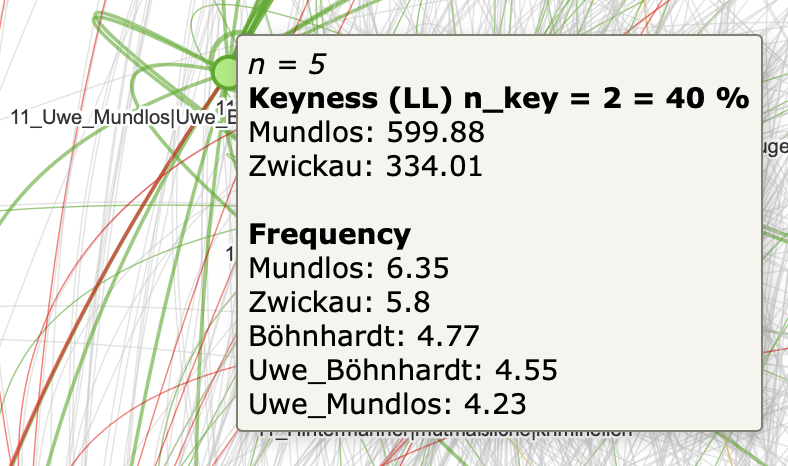
\includegraphics[width=\textwidth]{figures/media/image21.png}
  \caption{\label{fig:cluster-tooltip-nsu-mundlos}Tooltip zum Cluster \cluster{11\_Uwe\_Mundlos{\breakbar}Uwe\_Böhnhardt{\breakbar}Böhnhardt.}}
\end{figure}

Entscheidend bei der Interpretation des Graphen ist es, die enthaltenen Cluster als FE bzw. Slots eines Extremismus-Frames zu lesen und die in ihnen gebündelten Wörter als mögliche Filler des Slots bzw. zugleich Frame-evozierende LE. So kann das in \figref{fig:cluster-tooltip-nsu-mundlos} gezeigte Cluster als Teil eines größeren NSU-Frames interpretiert werden, in dem insbesondere die Mitglieder Uwe Böhnhardt und Uwe Mundlos, aber auch Zwickau als Wohnort des NSU enthalten sind. Ausdrücke wie \emph{Mundlos}, \emph{Zwickau} und \emph{Böhnhardt} wären dann dieses FE evozierende LE und zugleich die frequentesten Filler des Slots auf Token-Frame-Ebene. Aufgrund der Rekursivität von Frames können auch FE selbst als Frames gelesen werden. Durch die Einbettung in den Extremismus-Frame sind sie dabei zugleich in Hinblick auf dieses Thema perspektiviert (siehe \chapref{kollokation-von-word-embedding-clustern-als-frame-relationen-und-perspektivierung-kollokationsnetzwerke-als-frames}). Richtlinie bei der Interpretation der WE-Cluster als FE ist es, den größten gemeinsamen semantischen Nenner der enthaltenen Wörter zu identifizieren. \tabref{tab:example_clusters} in \chapref{geclusterte-word-embeddings-als-frame-elemente} zeigte bereits eine Auswahl von Clustern, die recht unkompliziert interpretierbar sind. Häufig sind Cluster jedoch, gerade wenn sie mehr Wörter umfassen, semantisch vager oder nur unter Ausblendung einzelner ‚Ausreißer` auf einen konzisen semantischen Nenner zu bringen. Dies betrifft etwa auch das zuvor genannte Cluster \cluster{11\_Uwe\_Mundlos{\breakbar}Uwe\_Böhnhardt{\breakbar}Böhnhardt}, das neben einem Teil der Mitglieder auch einen der Wohnorte des NSU enthielt oder mehr noch das Cluster \cluster{11\_Terrorzelle{\breakbar}Zwickauer\_Zelle{\breakbar}Zwickauer\_Terrorzelle}, das mit insgesamt 27 Wörtern größer ist und den NSU einerseits explizit in Hinblick auf Terror (u.\,a. \emph{Terrorzelle}, \emph{Rechtsterroristen}, \emph{Zwickauer\_Terrorzelle}) und Rechtsextremismus (u.\,a. \emph{rechten\_Szene}, \emph{rechtsextremen}) framet; andererseits aber auch Unterstützer des NSU wie \emph{Holger\_G} und \emph{Carsten\_S} enthält. Es findet sich dabei auch ein Mörder, der -- abgesehen von der durch die Handlung begründeten paradigmatischen Ähnlichkeit -- in keinem Zusammenhang zum NSU steht (\emph{Thomas\_S}). Das FE ist also insgesamt etwas vager als das zuvor betrachtete Cluster. Daran zeigt sich auch, dass nicht zu erwarten ist, etwa alle Akteure eines NSU-Frames im selben Cluster zu finden. Dies liegt darin begründet, dass sie jeweils in unterschiedliche Syntagmen eingebettet und mithin unterschiedlich geframet werden. Anschaulich macht das auch das wiederum separate Cluster \cluster{11\_Beate\_Zschäpe{\breakbar}Zschäpe{\breakbar}Nsu}, das neben diesen drei Ausdrücken auch das Wort \emph{Bundesanwaltschaft} enthält. Dieses FE ist deutlich stärker in den Bereich des juristischen Vokabulars eingebunden, da über Beate Zschäpe ausführlich als Hauptangeklagte im NSU-Prozess berichtet wurde. Am Beispiel des Clusters \cluster{08\_Intoleranz{\breakbar}Homophobie{\breakbar}Fremdenfeindlichkeit} wiederum zeigt sich, dass es wichtig ist, auch über das Cluster-Label hinaus Wörter bei der Interpretation einzubeziehen. So enthält das Cluster neben weiteren diskriminierungsbezogenen Wörtern (\emph{Diskriminierung}, \emph{Ausgrenzung}), auch Ausdrücke wie \emph{Gentrifizierung}, \emph{Hetze} oder \emph{Aggression}, die also auch andere negativ bewertete gesellschaftliche Handlungen bzw. Prozesse, die mehr oder weniger gegen Menschen gerichtet sind, umfassen.

Aufgrund der sehr hohen Knotenanzahl von 450--1413 Clustern pro Teilkorpus wäre eine Annotation der Cluster nur bei sehr umfangreichen Projekt-Ressourcen möglich. Wesentlich realistischer -- und so auch hier praktiziert -- ist es, die Interpretation der Cluster \emph{ad-hoc} vorzunehmen und einzelne Cluster nur dann im Detail zu untersuchen, wenn sie wesentlicher Bestandteil der Analyse werden. Als Beispiel mag der Hanau-Frame dienen (siehe \figref{fig:hanau-frame-2020-21} in \chapref{kollokation-von-word-embedding-clustern-als-frame-relationen-und-perspektivierung-kollokationsnetzwerke-als-frames}). Für eine erste Interpretation genügt es hier, sich einen Überblick über die angeschlossenen FE zu verschaffen. Es lässt sich, ohne die genauere Zusammensetzung der einzelnen Cluster wie \cluster{20\_tötete{\breakbar}tötet{\breakbar}erschoss}, \cluster{20\_Schmerz{\breakbar}Trauer{\breakbar}Scham} oder \cluster{20\_Gedenkfeier{\breakbar}Gedenkveranstaltung{\breakbar}Trauerfeier} zu betrachten, bereits mit großer Wahrscheinlichkeit sagen, dass es bei ersterem um die extremistische Gewalthandlung des Anschlags geht; bei zweiterem um emotionale Reaktionen auf den Anschlag sowie bei letzterem um Reaktionen in Form eines Gedenken an die Opfer des Anschlags. Diese wahrscheinlichen Vermutungen können zudem über einen Blick auf die an die jeweiligen FE angeschlossenen Cluster sowie die in den Tooltips ersichtlichen weiteren enthaltenen Wörter abgesichert werden. Dass dies funktioniert, liegt an der Kontextualisierungsleistung von Syntagmen und Paradigmen, die in der Methode aufgeht. Sollten auf diese Weise nur schwer interpretierbare Verbindung für die weitere Analyse relevant erscheinen, müsste die Verbindung der beiden Cluster näher geprüft werden: Welche der enthaltenen Wörter kookkurrieren hier tatsächlich (dies ist quantitativ überprüfbar) und worin besteht die Frame-Relation zwischen beiden Clustern (hier kann bei überschaubaren Frequenzen etwa eine Konkordanzsuche einen guten Überblick geben).

Während die Interpretation eines Knoten als FE einfach ist, wenn das Cluster sehr klein ist und womöglich nur ein Wort enthält -- in diesem Falle ist es in aller Regel sinnvoll, das Wort als FE bzw. Frame-Namen aufzufassen, etwa \cluster{20\_Hanau} und seine angeschlossenen FE als Hanau-Frame zu begreifen --, sind auch sehr große Cluster mit zum Teil über 8000 Wörtern im Graphen enthalten (z.\,B. \cluster{sp\_Gurgeltests{\breakbar}Zustellungen{\breakbar}Familienzusammenführungen}). Diese sind kaum sinnvoll interpretierbar und enthalten fast ausschließlich niedrigfrequente Wörter. Da diese FE häufig nicht im Sinne ihres zunächst kongruent erscheinenden Labels gedeutet werden können, sind alle Cluster mit mehr als 100 Wörtern im Graphen als Raute und alle Cluster mit über 200 Wörtern als Stern dargestellt. Weitere Möglichkeiten, mit diesen Clustern zu verfahren, werden in \chapref{methodische-limitationen-und-perspektiven} skizziert.

\subsubsection{Interpretation der Kanten}\label{interpretation-der-kanten}

Die Kanten des Graphen entsprechen aus Frame-semantischer Perspektive Frame-Relationen. Aus technisch-methodischer Perspektive sind sie zunächst \emph{Log-Likelihood}-Kollokationswerte, die zwischen den Wörtern der einzelnen WE-Cluster bestehen. Da die Darstellung aller statistisch signifikanten Kollokationsbeziehungen als Kanten zu einem hochgradig vernetzten und kaum mehr zu überblickenden Graphen geführt hätte, werden nur die jeweils 20 signifikantesten Kollokationspartner über eine Kante an einen Knoten angebunden, was zudem die Relevanz der Beziehung annäherungsweise abbildet. Genauso bedeutsam wie eine Kante zwischen zwei Knoten kann dabei auch das Ausbleiben einer solchen Verbindung sein. In dem Fall werden zwei FE, zumindest im zugrunde gelegten Kollokationsfenster, nicht in Beziehung zueinander gesetzt. Zum Beispiel werden im ungefähren Zeitraum 2002 bis 2010 FE wie \cluster{05\_Attentate{\breakbar}Attentaten{\breakbar}Bombenanschlägen} oder \cluster{08\_Gefährdung{\breakbar}Bedrohung{\breakbar}Störung} nicht in Verbindung zu Clustern des Rechtsextremismus gesetzt. Inwiefern in dieser Zeit, in der keine größeren (als solche erkannten) rechtsextremen Anschläge stattgefunden haben, entsprechende FE noch als Teil des gesellschaftlichen Wissens zu Rechtsextremismus gelten können, ist auf Basis der Daten nicht ohne Weiteres zu entscheiden. Ob also von einer Nullinstantiierung bzw. einem Default-Wert auszugehen ist, bei der die Frame-Relation so sehr im verstehensrelevanten Wissen verankert ist, dass sie nicht mehr verbalisiert wird, ist bei Fällen, wo das Ausbleiben einer solchen Beziehung überrascht, im Einzelfall nachzuprüfen und hermeneutisch zu entscheiden. Im genannten Fall erscheint dies jedoch eher unplausibel, da mit Aufdeckung des NSU im Jahr 2011 entsprechende Framing-Muster in aller Deutlichkeit zurückkehren und mithin wohl kein selbstverständlicher Teil des verstehensrelevanten Wissens mehr waren.

Auch die Interpretation der Kanten als Frame-Relationen muss in der Regel \emph{ad-hoc} und auf der Basis von Vorwissen erfolgen. Dies ist im Falle eines Clusters wie \cluster{we\_Kampf\_gegen} und den angeschlossenen Kanten in weiten Teilen gut möglich. Die angeschlossenen Frame-Elemente \cluster{we\_Missbrauch}, \cluster{we\_Armut}, \cluster{we\_Virus}, \cluster{we\_Terrorismus{\breakbar}Terror} sind häufige Objekte der Bekämpfung, Frame-Elemente wie \cluster{we\_Strategie}, \cluster{we\_Anstrengungen} oder \cluster{we\_Bemühungen} spezifizieren, wie und dass ein Kampf gegen etwas geführt wird. Nicht gleichermaßen eindeutig verhält es sich im Falle angeschlossener Akteure wie \cluster{we\_Extremisten{\breakbar}Dschihadisten{\breakbar}Terroristen} oder \cluster{we\_Terrormiliz{\breakbar}Al-kaida{\breakbar}Kabul}, die ja gleichermaßen Objekt der Bekämpfung als auch das den Kampf gegen etwas führende Subjekt sein können.

\largerpage
Zwei weitere potenziell bedeutungstragende Elemente sind im Graphen angelegt, da sie Informationen für die algorithmische Berechnung der Graph-Struktur bieten. Sie sind jedoch bei den hohen hier verwendeten Knotenanzahlen kaum in der Visualisierung erkennbar und werden auch in der Analyse keine weitere Berücksichtigung finden. Dies betrifft zum einen die Gerichtetheit der Kanten, die auf den ihrerseits gerichteten Kollokationen beruhen. Zwar kann es bedeutend sein, wenn sich ein Cluster unter den 20 signifikantesten Kollokatoren eines anderen Clusters findet, die Kollokation in die andere Richtung jedoch nicht gleichermaßen signifikant ist; aus Gründen der Komplexitätsreduktion kann dies jedoch in der Analyse nicht weiter berücksichtigt werden. Visuell ist diese Information zwar im Graphen enthalten, gleichwohl aufgrund ihrer geringen Bedeutung für die Analyse nur dezent markiert. So verlaufen im Fall einer beidseitig gerichteten Kollokation zwei Kanten zwischen den beiden Knoten, was aber nur bei starkem Zoom ersichtlich ist. Das zweite bei der Berechnung zugrunde gelegte, jedoch nicht sehr deutlich hervortretende Element ist die auf dem \emph{Log-Likelihood}-Wert beruhende Stärke der Verbindung zwischen zwei Knoten, die durch die Breite der Kante angezeigt wird. Hier sind nur die über alle Werte gesehen besonders signifikanten Verbindungen durch breitere Kanten gut sichtbar, häufig im thematischen Bereich Politik (z.\,B. die Kanten um das Cluster \cluster{we\_Cdu{\breakbar}Union}). Inwiefern andere Knoten eher starke oder eher schwache Verbindungen aufweisen, ist jedoch kaum zu erkennen. Dieses Problem wird dadurch gemindert, dass z.\,B. im Teilkorpus 2002--2004 mit einem mittleren \emph{Log-Likelihood}-Wert von 558,17 (arithmetisches Mittel) bzw. 194,93 (Median) und einem Minimum von 8,33 ohnehin alle dargestellten Kollokationen äußerst stark sind.

\subsubsection{Interpretation der räumlichen Struktur}\label{interpretation-der-raeumlichen-struktur}

Neben den Knoten und Kanten ist auch die räumliche Struktur des Graphen bedeutungstragendes Element der Visualisierung und soll im Folgenden beschrieben werden.

Insgesamt weisen die Netzwerke eine annähernd runde Struktur auf, die durch mindestens vier, mitunter auch einzelne weitere, Cluster bzw. Communities geprägt ist. Die Bildung der Communities beruht auf einer besonders hohen Vernetzung unter den jeweils enthaltenen Knoten, denn Knoten sind umso näher beieinander positioniert, je ähnlicher ihre Verbindungen sind. Hier schlägt sich also erneut eine paradigmatische distributionelle Ähnlichkeit nieder, sodass semantisch ähnliche Knoten häufig in der Nähe voneinander zu finden sind und sich auch innerhalb der Netzwerk-Cluster kleinere thematische Cluster bilden, so z.\,B. in der Community ‚Straftaten \& Juristisches` eine Gruppe mit Knoten wie \cluster{ta\_Gefängnis}, \cluster{ta\_Knast} und \cluster{ta\_Festnahmen{\breakbar}Verhaftungen}, eine andere mit Knoten wie \cluster{ta\_Ermittler}, \cluster{ta\_Ermittlern} und \cluster{ta\_Verdacht} sowie eine weitere mit Clustern wie \cluster{ta\_Klägerin{\breakbar}Kläger{\breakbar}Richterin}, \cluster{ta\_Berufung{\breakbar}Revision} oder \cluster{ta\_Richter{\breakbar}Staatsanwalt}. Auch die Positionierung einzelner Knoten im Verhältnis zu den Communities kann gemäß dem probabilistischen Charakter der Methode fruchtbar gedeutet werden. Zwar ist jeder Knoten zunächst durch den Algorithmus nur einer der Communities zugeordnet, jedoch graduell auch mit anderen Communities mehr oder weniger vernetzt, was sich durch die räumliche Nähe zu ebendiesen ausdrückt. Besonders sichtbar wird dies an den Knoten, die am Übergang von zwei Communities positioniert sind. Diese lassen sich i.d.R. auch semantisch beiden Communities zuordnen, so z.\,B. die Cluster \cluster{14\_Antrag} und \cluster{14\_Ausschuss{\breakbar}Untersuchungsausschuss{\breakbar}NSA-Untersuchungsausschuss}, die am Übergang zwischen den Communities ‚Politik` und ‚Straftaten \& Juristisches` verortet sind oder die Cluster \cluster{08\_beteiligt\_gewesen} und \cluster{08\_getötet{\breakbar}erschossen} am Übergang der Communities ‚Krieg \& Islamismus' und ‚Straftaten \& Juristisches`.

\subsubsection{Mögliche Fallstricke bei der Interpretation}\label{moegliche-fallstricke-bei-der-interpretation}

In diesem Kapitel sollen -- mitunter bereits angedeutete -- Missverständnisse zusammengefasst werden, die bei der Interpretation der erzeugten Frames auftreten können.

Das erste mögliche Problem betrifft die analytische Fokussierung auf einzelne Datenpunkte. Die hier vorgestellte Methode bietet einen Zugang zur epistemischen Makrostruktur von Diskursen im Sinne einer Vogelperspektive auf Diskurse und des \emph{distant reading} \autocite{morettiConjecturesWorldLiterature2000}. Alle Datenpunkte (einzelne Word Embeddings, Word-Embedding-Cluster, Kollokationen zwischen den Clustern, etc.) sind zudem einem relationalen, probabilistischen Zugang entsprechend berechnet und zu deuten, d.\,h. es spielen immer Ambiguitäten und die Komplexität vieler simultaner Relationen sowie auch Zufälligkeiten eine Rolle. Letztere gehen insbesondere auf die Nicht-Determiniertheit der verwendeten Algorithmen zurück. Die Berechnung von Word-Embeddings, das Clustering ebendieser, die Visualisierung der Word-Embedding-Cluster und ihrer Kollokationswerte als Graph, und die Erkennung von Clustern im Graph nutzen Algorithmen, die -- im Gegensatz zu z.\,B. der Berechnung von Kollokationen -- Zufallskomponenten beinhalten. Zwar werden dabei im Großen und Ganzen sehr ähnliche Ergebnisse erzielt, wenn die Methoden bei identischen Parametern auf dieselben Daten angewandt werden. Einzelne Datenpunkte können jedoch durchaus unterschiedlich berechnet werden. So können etwa einzelne Word-Embeddings leicht andere nächste Nachbarn im Vektorraum haben oder in andere Cluster gezählt werden. Es wäre aus diesem Grund voreilig, Analyseschlüsse auf Detail-Ergebnissen dieser Algorithmen zu stützen. Zum Beispiel sollte daraus, dass in Cluster \cluster{20\_Susanne\_Hennig-Wellsow{\breakbar}Hennig-Wellsow{\breakbar}Mike\_Mohring} neben den thüringer Politiker*innen Susanne Hennig-Wellsow und Mike Mohring auch die Wörter \emph{Gauland}, \emph{Franziska\_Giffey} und \emph{Chrupalla} enthalten sind, noch nicht geschlossen werden, dass jede einzelne dieser Politiker*innen eine ähnliche Rolle im Extremismusdiskurs spielt und sich von benachbarten Clustern wie \cluster{20\_Schäuble{\breakbar}Bouffier{\breakbar}Dobrindt} oder \cluster{20\_Höcke{\breakbar}Kalbitz{\breakbar}Andreas\_Kalbitz} deutlich unterscheidet. Zwar zeichnet sich ab, dass das letztgenannte Cluster insbesondere AfD-Politiker und -Strukturen beinhaltet und das erstgenannte in weiten Teilen die Ereignisse um die Thüringer Ministerpräsidentenwahl 2020 widerspiegelt; warum aber z.\,B. \emph{Chrupalla} in dieses Cluster und nicht ins AfD-Cluster sortiert wurde, ist nicht auf den ersten Blick ersichtlich. Es ist außerdem wahrscheinlich, dass sich bei erneuter Berechnung der Cluster einzelne Cluster nicht erneut bilden bzw. andere Wörter umfassen. Dies bedeutet nicht, dass nicht tatsächlich Unterschiede in der Semantisierung bestehen. Sie sind sogar wertvolle Hinweise darauf, denen im Sinne einer datengeleiteten, quantitativ informierten Diskursanalyse \autocite{bubenhoferQuantitativInformierteQualitative2013} weiter nachgegangen werden kann. Sie müssten aber zunächst durch ergänzende Analysen weiter abgesichert werden (s.u.). Für die makrostrukturelle Diskursbeschreibung ist es hingegen empfehlenswert, Muster zu identifizieren, die über den einzelnen Datenpunkt hinausgehen. Dies können zum einen rekurrente Muster wie das in allen Teilkorpora bestehende Cluster um Wortformen der Lexeme \emph{antisemitisch}, \emph{rassistisch} und \emph{rechtsextrem} bzw. \emph{rechtsextremistisch} (z.\,B. \cluster{05\_rechtsextremen{\breakbar}rechtsextremistischen{\breakbar}rechtsextreme}, \cluster{14\_rechtsradikale{\breakbar}rechtsradikalen{\breakbar}Rechtsradikalen} oder \cluster{ta\_rechtsradikale{\breakbar}rechtsextreme{\breakbar}antisemitische}) sein. Dieses wiederkehrende Muster zeigt deutlich an, dass wesentliche Eigenschaften des Rechtsextremismus als solche im gesellschaftlichen Wissen verankert sind und sprachlich realisiert werden. Zum anderen ist es empfehlenswert, größere zusammenhängende Strukturen wie die als Extremismus-Varianten-Frames lesbaren Verbünde aus Knoten des Graphen zu fokussieren. Es kann auch nur so das rekontextualisierende Potenzial \autocite{bubenhoferVisuelleLinguistikZur2020} der verwendeten Methode bzw. Visualisierung erfasst und für die Analyse fruchtbar gemacht werden. Dies gilt grundsätzlich auch für die auf Kollokationen beruhenden Kanten; sie sind den angesprochenen Unsicherheiten jedoch nur in geringerem Maße unterworfen, da sie ein algorithmisch-deterministisches methodisches Element darstellen.

Ein weiterer möglicher Fallstrick, der bereits in \chapref{geclusterte-word-embeddings-als-frame-elemente} in Kürze angesprochen wurde, betrifft die Interpretation der Word-Embedding-Cluster als FE. Hier ist insbesondere zu berücksichtigen, dass Cluster weit mehr Wörter enthalten können als nur die drei Wörter, die das Label des Clusters ausmachen. So beinhaltet etwa das Cluster \cluster{99\_wirtschaftlichen{\breakbar}ökonomischen{\breakbar}ökonomische} neben den drei namensgebenden, im Vektorraum zentralsten Wörtern des Clusters und den semantisch kongruenten Wörtern \emph{wirtschaftliche} und \emph{finanziellen} auch die Ausdrücke \emph{Globalisierung}, \emph{ökologische} und \emph{ökologischen}. Während das Label des Clusters also zunächst eine Interpretation als rein wirtschaftsbezogenes FE nahelegt, sind auch Aspekte der Ökologie und Globalisierung im Cluster enthalten. Letztlich beruht jedoch die Nachbarschaft im Vektorraum und mithin die Zuordnung zu einem gemeinsamen Cluster auf dem musterhaften Auftreten in ähnlichen Kontexten und es ist durchaus sinnvoll, das Wort \emph{Globalisierung} als stark assoziiert mit ökonomischen und ökologischen Fragen zu sehen. Insofern ist es an dieser Stelle empfehlenwert, das Cluster zunächst als eher vages Frame-Element zu lesen, das insgesamt den Bereich von Ökologie, Ökonomie und Globalisierung betrifft. Wann immer die genaue Beziehung des FE zu anderen FE von Interesse ist, müssten genauere Analysen erfolgen, welche Wörter der beiden Cluster tatsächlich kookkurrieren.

Hiermit ist zugleich ein weiterer möglicher Fehlschluss angesprochen, der bei der Interpretation des Graphen gemacht werden kann und die Kanten bzw. Frame-Relationen betrifft. So beruhen die eingezeichneten Kanten ja auf Kollokationen der Wörter des einen Clusters mit Wörtern des anderen Clusters, wobei die einzelnen Wörter und ihr individuelles Kollokationsverhalten nicht mehr berücksichtigt werden. Hierdurch wirken sich frequentere Wörter auch stärker auf die Kollokationen des Clusters aus als weniger frequente Wörter. Einzelne Verbindungen können also eher durch einzelne Wörter geprägt sein sowie insgesamt eher durch die frequenteren Wörter des Clusters.\footnote{Insgesamt liegt den Word-Embedding-Clustern jedoch eine paradigmatische Ähnlichkeit zugrunde, sodass grundsätzlich von einem ähnlichen Kollokationsverhalten der Wörter auszugehen ist (siehe \chapref{was-sind-word-embeddings}).} Des Weiteren ist bei der Interpretation der Kanten zu beachten, dass nur die 20 signifikantesten Kollokationen eines jeden WE-Clusters an es angebunden sind (siehe auch \chapref{berechnung-des-extremismus-centroid-und-begrenzung-der-knotenmenge}). Besteht also zwischen zwei Knoten keine Kante, bedeutet dies nicht, dass nicht auch diese Cluster signifikant kookkurrieren. Sie sind nur jeweils nicht unter den Top-Kollokatoren des anderen Clusters vertreten. Die genauen Kollokationsdaten sind bei Bedarf über die Korpussoftware abrufbar.

\largerpage
Letztlich ist noch einmal auf einen Nachteil der auf \emph{Word2Vec} und ähnlichen Algorithmen basierenden Word Embeddings hinzuweisen. Wie in \chapref{was-sind-word-embeddings} dargestellt, handelt es sich bei ihnen um Type-basierte Algorithmen, die also für jeden Korpus-Type im Sinne eines formseitig identischen Tokens eine Vektorrepräsentation berechnen. Bei der Berechnung werden alle Belegstellen für diese Types herangezogen, was bei homonym bzw. polysem oder metonymisch gebrauchten Wörtern ein Problem darstellen kann. Sind etwa Wörter wie \emph{Björn\_Höcke}, \emph{Andreas\_Kalbitz} und \emph{Flügel} im Cluster \cluster{20\_Höcke{\breakbar}Kalbitz{\breakbar}Andreas\_Kalbitz} zusammengefasst, beruht das darauf, dass \emph{Flügel} als Name einer Parteistruktur gebraucht wird und daher nicht etwa mit Wörtern wie \emph{Schwingen}, \emph{Schnabel} oder \emph{Federn} zusammengefasst ist, die das Wort noch im Zeitraum 2011--2013 im Vektorraum umgeben. Interessant -- aber auch komplexitätssteigernd -- wäre es, unterschiedliche Embeddings für die Bedeutungen zu haben, was im Rahmen der hier verwendeten Algorithmen jedoch nicht ohne Weiteres zu realisieren ist. Grundsätzlich wäre auch denkbar, dass homonyme Wörter bei sehr unterschiedlichen Verwendungskontexten gar keine sinnvolle Vektorrepräsentation erhalten und somit für die Analyse nicht nutzbar sind. Dass Wörter im Korpus gleichermaßen in unterschiedlichen Bedeutungen vorkommen, ist jedoch aufgrund der korpuspragmatischen Kontextualisierung eher unwahrscheinlich. So kommt das Wort \emph{Bank} in Zeitungstexten in aller Regel in seiner Bedeutung als Finanzinstitut, nicht als Sitzgelegenheit vor. Folglich sind seine nächsten Nachbarn im Vektorraum des Zeitraums 2020--2021 \emph{Sparkasse}, \emph{Commerzbank} und \emph{Greensill}.\footnote{Ein Beispiel für ein durch Polysemie geprägtes paradigmatisches Profil ist das Umfeld des Wortes \emph{Flügel} im Word-Embedding-Modell 2014--2016. Unter den 10 nächsten Nachbarn finden sich sowohl \emph{rechten\_Flügel}, \emph{linken\_Flügel} und \emph{Parteiflügel}, die auf einen eher politischen Gebrauch hindeuten; \emph{Saiten}, was auf das Musikinstrument deutet sowie \emph{Propeller}, was den Gebrauch des Wortes \emph{Flügel} in der Luftfahrt widerspiegelt.} Neben der übergreifenden Disambiguierung durch den medialen Kontext bietet auch die diachrone Unterteilung des Korpus dieses Potenzial. So können die Wörter, die nicht konstant mehrdeutig gebraucht werden, durch das Kriterium der thematischen Einschlägigkeit in die Frame-Modellierung ein- oder ausgeschlossen werden. Wörter wie \emph{Hanau}, \emph{Querdenker} oder \emph{Lkw} sind dann nur in den Jahren, in denen sie für die Modellierung eines Extremismus-Frames relevant sind, in der Darstellung enthalten. Auch da die jeweils angeschlossenen Kanten ebenfalls thematisch in Hinblick auf Extremismus perspektiviert sind, wird nicht unnötigerweise das gesamte Bedeutungsspektrum eines Ausdrucks im Frame aufgefächert.
 %typeset
\chapter{Analyse}\label{analyse}

\section{Vorgehen und Zielsetzung}\label{vorgehen-und-zielsetzung}

Die Analyse wird mithilfe der vorgeschlagenen Methode \emph{corpus-driven} ermittelte Frame-Strukturen\footnote{Die Visualisierungen sind unter \url{https://doi.org/10.5281/zenodo.14216890} abrufbar.} auf unterschiedlichen Ebenen herausarbeiten. Im Sinne eines induktiven Ansatzes geht sie von der datengeleiteten Beschreibung der Makrostruktur der Frames zur sowohl \emph{corpus-driven} als auch \emph{corpus-based} vorgenommenen Analyse der Extremismusvarianten-Frames.

In der makrostrukturellen Analyse wird zunächst die Netzwerk-Cluster bildende Gesamtstruktur der Frames in den Blick genommen und als thematische Teil-Frames interpretiert. Anschließend erfolgt die Untersuchung der Mesostruktur des Frames. Dabei wird entlang der Knoten, die für eine Extremismusvariante besonders einschlägig sind, möglichst ein Frame pro Extremismusform (Rechts- und Linksextremismus sowie Islamismus) erschlossen, wobei nicht in jedem Teilkorpus alle Formen deutlich zu Tage treten. Die Selektion der einschlägigen FE ist dabei ein Element der Analyse, das stärker durch Vorwissen geleitet ist als die übrigen Verfahrensschritte. Es werden solche FE ausgewählt, die auf relativ unstrittige Weise einen Extremismus-Frame evozieren. Dazu zählen insbesondere Cluster wie z.\,B. \cluster{11\_Neonazis{\breakbar}Rechtsextremisten{\breakbar}Rechtsextremen}, \cluster{we\_Extremisten{\breakbar}Dschihadisten{\breakbar}Terroristen} oder \cluster{09\_Fremdenfeindlichkeit{\breakbar}Ausländerfeindlichkeit{\breakbar}Rassismus}, die also unstrittige Bezüge zum Extremismusdiskurs als z.\,B. Akteure, Charakteristika oder den Frame-Namen selbst enthaltende Ausdrücke aufweisen. Die \emph{corpus-based} Selektion dieser Kern-FE wird jedoch durch eine Vielzahl emergentistischer Elemente flankiert. So erfolgen zunächst für jedes Teilkorpus zwei \emph{corpus-driven} Voranalysen. Es werden zum einen unter allen Clustern des Zeitraumes diejenigen identifiziert, die im Vergleich zum Vorjahreszeitraum die größte Cosinus-Distanz aufweisen. Da sich die Cluster zwischen den Subkopora unterscheiden, wird für jedes Wort eines Clusters die Distanz zum Vektor desselben Ausdrucks im Vorjahreszeitraum ermittelt und dann das arithmetische Mittel dieser Wort-Distanzen berechnet. Die zweite Voranalyse besteht in der Berechnung der fünf semantisch äquivalentesten, d.\,h. im Vektorraum nächsten, Cluster zu den im Vorjahreszeitraum als Kern-FE betrachteten Clustern, wobei die Distanzen zwischen den jeweiligen Cluster-Centroids zugrunde gelegt werden. Die große Anzahl der so identifizierten FE wird im Anhang gelistet (Tabellen 3--10) und zu Beginn jedes Analysekapitels zusammengefasst und thematisch gruppiert. Bei beiden Analysen werden sehr große Cluster von mindestens 100 Wörtern aus den Ergebnissen gefiltert, da sie für die Analyse i.d.R. nicht interessant sind (siehe \chapref{interpretation-der-knoten}) und aufgrund ihres semantisch disparaten Charakters häufig auf den vorderen Rängen der Analyseergebnisse auftauchen.

Des Weiteren werden zu den Varianten-Frames nicht nur die Kern-FE, sondern auch alle an sie angeschlossenen FE gezählt und bei der Analyse miteinbezogen, sodass die Gesamtstruktur weit über die manuell ausgewählten FE hinausgeht. Eine Voraussetzung für die Selektion der FE besteht außerdem in einer Vernetztheit mit anderen Frame-Bestandteilen. Es werden also keine FE einbezogen, die intuitiv dem Diskurs zugehörig erscheinen würden, jedoch keinen Zusammenhang in der Frame-Struktur aufweisen. Der Grund für die Nutzung von \emph{corpus-driven} methodischen Elementen besteht dabei nicht nur im allgemeinen Vorhaben dieser Arbeit, die Potenziale ebendieser Verfahren auszureizen. Es geht auch darum, möglichst alle relevanten FE einzubeziehen, was in einem stark von Vorwissen bzw. Hypothesen geprägten Vorgehen gefährdet ist. Erstens besteht der Vorteil von datengeleiteten Verfahren ja gerade in ihrem Potenzial, auch Unerwartetes freizulegen; zweitens sind mit der Wahl eines quantitativen Zugangs, eines sehr großen Korpus und eines recht langen Untersuchungszeitraum sowie der Berechnung feingranularer Frame-Strukturen bereits Entscheidungen getroffen worden, die mit qualitativ und/oder \emph{corpus-based} ausgericheteten Zugängen schwer vereinbar sind. Zu umfangreich sind die vorliegenden Daten, als dass sie durch rein manuelle Analysen noch zu bearbeiten wären.

Die Zielsetzung der Analyse besteht darin, die entwickelte Methode am Extremismusdiskurs zu erproben und das Framing einzelner Extremismusvarianten im diachronen und medienkontrastiven Vergleich auf einer Makro- und Mesoebene herauszuarbeiten. Aufgrund des vordergründigen methodologischen Interesses der Arbeit ist die Analyse dabei zu fokussieren und kann nicht exhaustiv erfolgen. Insbesondere die Mikroebene, auf der etwa einzelne FE oder lexikalische Einheiten sowie qualitativere Analysen ins Blickfeld rücken könnten, kann im Rahmen dieser Arbeit keine Beachtung finden. Durch die illustrative Einbindung von Konkordanzen und Analysen zu einzelnen FE werden sich die Potenziale aber zumindest abzeichnen. Vor dem Hintergrund der Komplexität der rekursiven Wissensstrukturen bzw. ihrer sprachoberflächlichen Korrelate ist es zudem notwendig, die Analyse auf wesentliche Veränderungen des Framings zu fokussieren. Insbesondere im Bereich des Islamismus können nur einige wesentliche Bestandteile des Frames schlaglichtartig herausgearbeitet werden, da eine angemessene Auseinandersetzung mit den zahlreichen Gruppierungen, Konflikten und Hintergründen des Islamismus im Nahen und Mittleren Osten sehr gute Kenntnisse des Diskurses bzw. bestenfalls die Bearbeitung durch ein interdisziplinäres Team erfordern würde.

Auch die Analyse der Zeitungsteilkorpora wird sich auf die kontrastive Analyse einiger gut vergleichbarer FE fokussieren und kann aufgrund der sehr umfangreichen Frame-Strukturen, deren Unterschiede im Kontrast nicht gleichermaßen gut zu erfassen sind, nicht umfangreicher erfolgen.\footnote{Problematisch ist insbesondere, dass die große Anzahl an FE (sie geringer anzusetzen, hätte jedoch zum Verlust thematisch einschlägiger Cluster geführt) für die Forschungsperson schwierig zu überblicken ist. Zugleich sind die Ergebnisse der quantitativen Voranalysen zu semantischen Veränderungen, die eine hohe Cluster-Anzahl grundsätzlich händeln können, im Falle der Zeitungskorpora kaum fruchtbar zu interpretieren. Die Entwicklung weiterer methodischer Elemente zur hermeneutischen Erschließung stellt also ein Desiderat dar.} Es werden dabei die in \tabref{tab:cluster_newspapers} gelisteten Cluster besonders in den Blick genommen. Es wurden solche Cluster ausgewählt, die einerseits stellvertretend für ein bestimmtes Thema sind und -- in möglichst vergleichbarer Form, d.\,h. ohne semantisch vager zu sein und deutlich mehr Ausdrücke zu umfassen -- auch in den beiden anderen Zeitungen emergent sind.\footnote{Dass so deutlich mehr \textsc{Taz}-Cluster betrachtet werden, liegt am in \chapref{politischer-extremismus} beschriebenen Fokus der Zeitung auf dem politischen Extremismus, der höhere Frequenzen und mithin differenziertere Cluster zur Folge hat.}

\begin{table}[t]\small
\caption{Zu betrachtende Cluster für den medialen Vergleich nach Extremismusvariante und thematischem Bezug.}
\label{tab:cluster_newspapers}
 \begin{tabularx}{\textwidth}{>{\hsize=0.5\hsize}X >{\hsize=0.5\hsize}X >{\hsize=2.0\hsize}X}
  \lsptoprule
  Extremismus-& Bezug & Frame-Elemente \\
  Variante & & \\
  \midrule
  \multirow{1}{=}{Rechts\-ex\-tre\-mis\-mus} & Politik & \cluster{ta\_Afd{\breakbar}Npd, ta\_Dvu, ta\_Schill{\breakbar}Schill-Partei, ta\_Gauland{\breakbar}Höcke{\breakbar}Meuthen (AfD-Politiker{\slash}Möllemann), ta\_Alexander\_Gauland{\breakbar}Jörg\_Meuthen{\breakbar}Poggenburg (Rechtsaußen-Politiker), sp\_Afd{\breakbar}Npd, sp\_Gauland{\breakbar}Petry{\breakbar}Höcke} \\
  & NSU & \cluster{ta\_Nsu, ta\_Zschäpe{\breakbar}Beate\_Zschäpe, sp\_Beate\_Zschäpe{\breakbar}Zschäpe{\breakbar}Nsu-prozess, sp\_Uwe\_Böhnhardt{\breakbar}Böhnhardt{\breakbar}Uwe\_Mundlos, we\_Uwe\_Böhnhardt{\breakbar}Uwe\_Mundlos{\breakbar}Böhnhardt, we\_Beate\_Zschäpe{\breakbar}Zschäpe{\breakbar}Nsu} \\
  & außer\-par\-la\-men\-ta\-risch & \cluster{ta\_Rechtsextremisten{\breakbar}Neonazis{\breakbar}Rechtsextremen, sp\_Neonazis{\breakbar}Rechtsextremisten{\breakbar}Rechtsextreme, we\_Rechtsextremisten{\breakbar}Neonazis{\breakbar}Rechtsextremen} \\
  \midrule
  \multirow{1}{=}{Links\-ex\-tre\-mis\-mus} & Politik & \cluster{ta\_Linke, ta\_Pds{\breakbar}Linkspartei, ta\_Oskar\_Lafontaine{\breakbar}Lafontaine{\breakbar}Gregor\_Gysi, sp\_Linkspartei{\breakbar}Pds{\breakbar}Linken, sp\_Lafontaine{\breakbar}Gysi{\breakbar}Oskar\_Lafontaine} \\
  & außer\-par\-la\-men\-ta\-risch & \cluster{ta\_gegen\_Rechts{\breakbar}antifaschistische{\breakbar}Antifa, ta\_Antifa-gruppen{\breakbar}Aktivistinnen{\breakbar}linke\_Gruppen, ta\_Heiligendamm{\breakbar}Genua{\breakbar}G-8-Gipfel, sp\_G-8-Gipfel{\breakbar}G7-Gipfel{\breakbar}G-20-Gipfel, we\_G-20-Gipfel{\breakbar}G-8-Gipfel{\breakbar}G-7-Gipfel} \\
  \midrule
  Islamismus & Islamischer Staat & \cluster{ta\_iS, sp\_Miliz{\breakbar}Milizen{\breakbar}Armee, we\_iS} \\
  \lspbottomrule
 \end{tabularx}
\end{table}

Wie in \chapref{interpretation-der-knoten} bereits skizziert, kann nicht für alle in den Frames enthaltenen Cluster eine explizite Interpretation als FE geleistet werden. Bei der analytischen Auseinandersetzung muss stattdessen auf das rekontextualisierende Potenzial \autocite{bubenhoferVisuelleLinguistikZur2020} der eingesetzten Methoden vertraut werden und die Interpretation der meisten der bis zu 1413 Cluster kann nur \emph{ad-hoc} und in Auseinandersetzung mit dem Cluster-Label bzw. den im Tooltip enthaltenen Wörtern geschehen. Erst wenn Cluster näher untersucht und die Basis für analytische Schlüsse darstellen, werden sie noch einmal näher in Hinblick auf die Gesamtheit der enthaltenen Wörter betrachtet und ihre Rolle im Frame wird in Klammern bzw. im Fließtext angegeben, so z.\,B. beim Cluster \cluster{05\_rechtsextremen{\breakbar}rechtsextremistischen{\breakbar}rechtsextreme (Extremismus)}. Anders als das Label vermuten lässt, beinhaltet das Cluster nicht nur attributive Bezugnahmen auf Rechtsextremismus, sondern spiegelt mit Ausdrücken wie \emph{gewaltbereiten}, \emph{Mob}, \emph{Hassprediger}, \emph{islamistische} oder \emph{militante} einen deutlich breiteren Teil der Extremismussemantik wider.

\largerpage
Letztlich ist hervorzuheben, dass die Analyse -- vor dem Hintergrund der „heillosen Sprachverwirrung`` \autocite[49]{backesVergleichendeExtremismusforschung2005} in der Extremismusforschung und der hochgradig wandelbaren Konzeptualisierungen von Extremismus (siehe \chapref{begriffliche-verwirrungen-und-kritik-am-extremismus-konzept} und \ref{extremismus-diskurs}) -- nicht das Ziel verfolgt, ein eng definitorisch vorgefasstes Verständnis von Extremismus abzubilden. Es werden also insbesondere bei der Selektion der Kern-FE keine Unterschiede zwischen ‚Extremismus`, ‚Radikalismus`, ‚Totalitarismus` und weiteren möglichen Ausdifferenzierungen gemacht, sondern vielmehr im Nachhinein analysiert, ob diese Unterschiede zu Tage treten. Um Missverständnissen vorzubeugen, sei auch darauf hingewiesen, dass intendiert ist, in den Frames einen größtmöglichen Teil des ‚gesamten verstehensrelevanten Wissens` im Sinne Busses abzubilden und die einzelnen FE sowie ihre Relationen im Frame interpretationsbedürftig sind. Dass sie in den Frame einbezogen wurden, bedeutet also zunächst nur, dass sie in irgendeiner Form Teil des Extremismusdiskurses sind -- nicht dass z.\,B. einzelne enthaltene Akteure oder Handlungen als extremistisch geframet werden oder gar extremistisch ‚sind`.\footnote{Letzteres Urteil wäre im Rahmen einer diskursanalytischen Arbeit, die sich ausschließlich damit beschäftigt, wie Wissen im Diskurs konstituiert und verhandelt wird, natürlich ohnehin nicht zu fällen.} Die Analyse wird außerdem in dem Bewusstsein vorgenommen, im Diskurs zu erwartende Framings -- etwa eine Gleichsetzung unterschiedlicher Extremismusformen, die von Kritiker*innen der Extremismustheorie immer wieder hervorgehoben wird -- zu reproduzieren. Damit verbunden ist jedoch der Gedanke, eine deskriptive Grundlage für anschließbare kritisch-diskursanalytische Auseinandersetzungen zu schaffen.

\section{Makrostruktur: Thematische Teil-Frames}\label{makrostruktur-thematische-teil-frames}
Im Folgenden wird die Makrostruktur der Frames im Sinne der \emph{corpus-driven} identifizierten Netzwerk-Communities, die als thematische Frame-Anteile operationalisiert wurden, analysiert (\chapref{netzwerk-communities-als-thematische-teil-frames} und \ref{visualisierung-als-netzwerk-graph-und-erkennung-von-communities}).

Es zeigen sich im Kontrast der insgesamt elf gebildeten Subkorpora sechs rekurrente Netzwerk-Communities, die algorithmisch identifiziert werden können. Neben den drei auch visuell erkennbaren, eher außen gelagerten Communities ‚Politik`, ‚Krieg \& Islamismus`, ‚Straftaten \& Juristisches`, ist es durch den algorithmischen Zugang möglich, weitere Cluster zu identifizieren, die aufgrund der sich überlagernden Frame-Strukturen andernfalls nicht erkennbar bzw. voneinander unterscheidbar gewesen wären und die sich den Themen ‚Staat, FdGO \& Gesellschaft`, ‚Demonstrationen \& politischer Extremismus` und ‚Außenpolitik` zuordnen lassen. Die sechs rekurrenten Cluster sollen im Folgenden vorgestellt werden.

\begin{figure}
  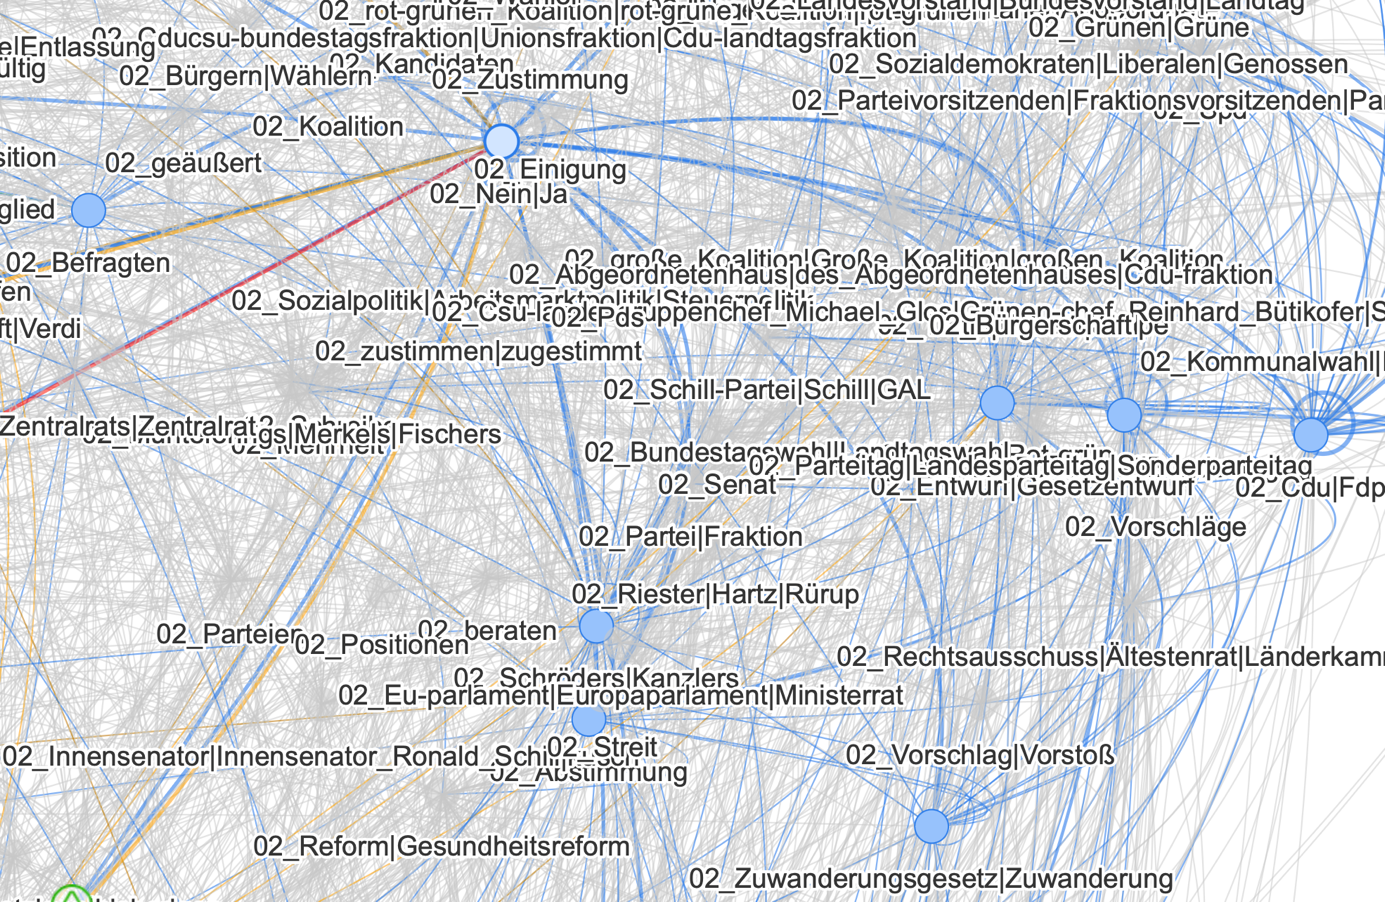
\includegraphics[width=\textwidth]{figures/media/image22.png}
  \caption{\label{fig:politik-beispiel}Ausschnitt aus dem thematischen Teil-Frame ‚Politik` am Beispiel des Clusters \cluster{02\_Nein{\breakbar}Ja}.}
\end{figure}

\largerpage[2]
Die Community ‚Politik` (\figref{fig:politik-beispiel}) umfasst (tages\mbox{-})politische Zusammenhänge. Die hier vertretenen Frame-Elemente umfassen insbesondere Akteure (z.\,B. \cluster{sp\_Afd{\breakbar}Npd}, \cluster{02\_Politiker{\breakbar}Kritiker}, \cluster{11\_Wähler}, \cluster{14\_Csu}) und Praktiken (z.\,B. \cluster{99\_Anhörung{\breakbar}Sondersitzung}, \cluster{02\_Wahl}, \cluster{14\_Debatte{\breakbar}Diskussion}) dieses Themenfeldes. Die Rolle der einzelnen FE im Extremismus-Frame kann dabei sehr unterschiedlich ausfallen. Akteure wie die NPD gelten selbst als extremistisch und sind einerseits wie alle politischen Parteien mit angeschlossenen FE wie \cluster{08\_Landtag}, \cluster{08\_Stimmen}, \cluster{08\_Parteitag} versehen. Die NPD weist aber auch eine starke Verankerung im Bereich der Demonstrationen (\cluster{08\_Demonstrationen{\breakbar}Kundgebung{\breakbar}Demo}, \cluster{08\_protestiert{\breakbar}demonstriert}) und mit anderen demonstrierenden Akteuren der rechten und linken Extreme (\cluster{08\_Autonomen{\breakbar}Antifas{\breakbar}Antifa}) sowie zu rechtsextremen Akteuren bzw. Attribuierungen (\cluster{08\_Rechtsextremisten{\breakbar}Neonazis{\breakbar}Rechtsextremen}, \cluster{08\_Fundamentalisten{\breakbar}rechtsradikalen{\breakbar}extremistische}) auf. Auch juristische Zusammenhänge wie \cluster{08\_Verbot} schlagen sich im Frame dieses Akteurs nieder. Andere politische Akteure wie \cluster{02\_Johannes\_Rau{\breakbar}Oskar\_Lafontaine{\breakbar}Helmut{\breakbar}Kohl} sind hingegen fast ausschließlich innerhalb der Community ‚Politik` vernetzt und werden nicht als extremistisch geframet. Es können außerdem politische Projekte bzw. Gesetzesänderungen in diesem Cluster verankert sein, so etwa das FE \cluster{02\_Agenda\_2010{\breakbar}Reformen{\breakbar}Hartz\_Iv}. Warum dieses vielleicht nicht ohne Weiteres für den Extremismusdiskurs einschlägige Cluster Teil des Frames ist, wird über die Betrachtung der angeschlossenen FE deutlich, die Aufschluss über das Framing der Reform geben. Vor allem die Vernetzung zum Bereich der Demonstrationen (\cluster{02\_Protest\_gegen{\breakbar}Protest}, \cluster{02\_Autonomen{\breakbar}Antifa{\breakbar}Rechtsextremisten}, \cluster{02\_Demonstrationen{\breakbar}Protestaktionen{\breakbar}Demos}, \cluster{02\_aufgerufen}) sowie den gesellschaftlichen Folgen der Gesetzesänderung (\cluster{02\_Zorn{\breakbar}Unmut{\breakbar}Wut}, \cluster{02\_Verwerfungen{\breakbar}Unsicherheiten{\breakbar}Unwägbarkeiten}) aufgrund des ausgeprägten außerparlamentarischen Protests gegen die Reform weist dabei Ähnlichkeiten zum Framing von Extremismus auf.

\begin{figure}[b]
  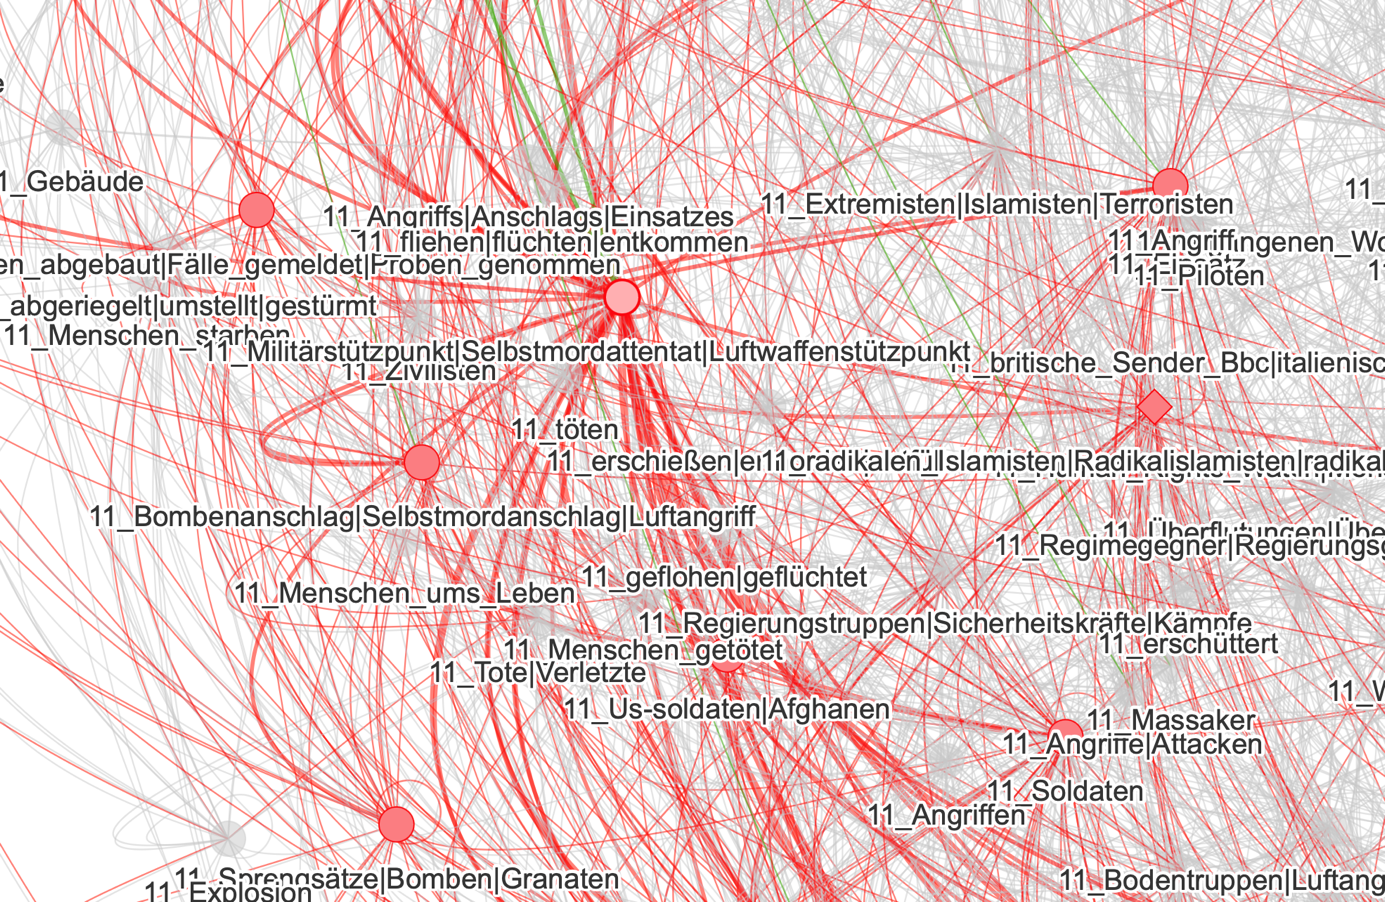
\includegraphics[width=\textwidth]{figures/media/image23.png}
  \caption{\label{fig:krieg-beispiel}Ausschnitt aus dem thematischen Teil-Frame ‚Krieg \& Islamismus` am Beispiel des Clusters \cluster{11\_Militärstützpunkt{\breakbar}Selbstmordattentat{\breakbar}Luftwaffenstützpunkt}.}
\end{figure}

Das Cluster ‚Krieg \& Islamismus` (\figref{fig:krieg-beispiel}) beinhaltet insbesondere kriegerische Handlungen (\cluster{02\_Tötung}, \cluster{14\_Luftschläge{\breakbar}Luftangriffe{\breakbar}Luftangriffen}, \cluster{we\_Angriffen}), Akteure (z.\,B. \cluster{02\_Iraker}, \cluster{11\_Regierungstruppen{\breakbar}Sicherheitskräfte{\breakbar}Kämpfe}, \cluster{14\_Bundeswehr}), Orte (z.\,B. \cluster{14\_Nordwesten\_Syriens{\breakbar}Nordosten\_Syriens{\breakbar}Norden\_Syriens}, \cluster{ta\_Gebiet}), Waffen und Kriegsgerät (z.\,B. \cluster{08\_Kampfjets{\breakbar}Kampfflugzeuge{\breakbar}Luftwaffe}, \cluster{we\_Handgranaten{\breakbar}Maschinengewehre{\breakbar}Pistolen}) sowie Attribute (z.\,B. \cluster{ta\_militärische{\breakbar}militärischen{\breakbar}militärischer}). Auch islamistische Handlungen (z.\,B. \cluster{14\_Anschläge{\breakbar}Terroranschläge{\breakbar}Attentate}, \cluster{14\_Attentäter{\breakbar}Selbstmordattentäter}) und Akteure (z.\,B. \cluster{08\_Extremisten{\breakbar}Taliban{\breakbar}Islamisten, 14\_IS\_Miliz{\breakbar}Terrormiliz{\breakbar}Isis}) fallen in dieses Netzwerk-Cluster.

\begin{figure}[t]
  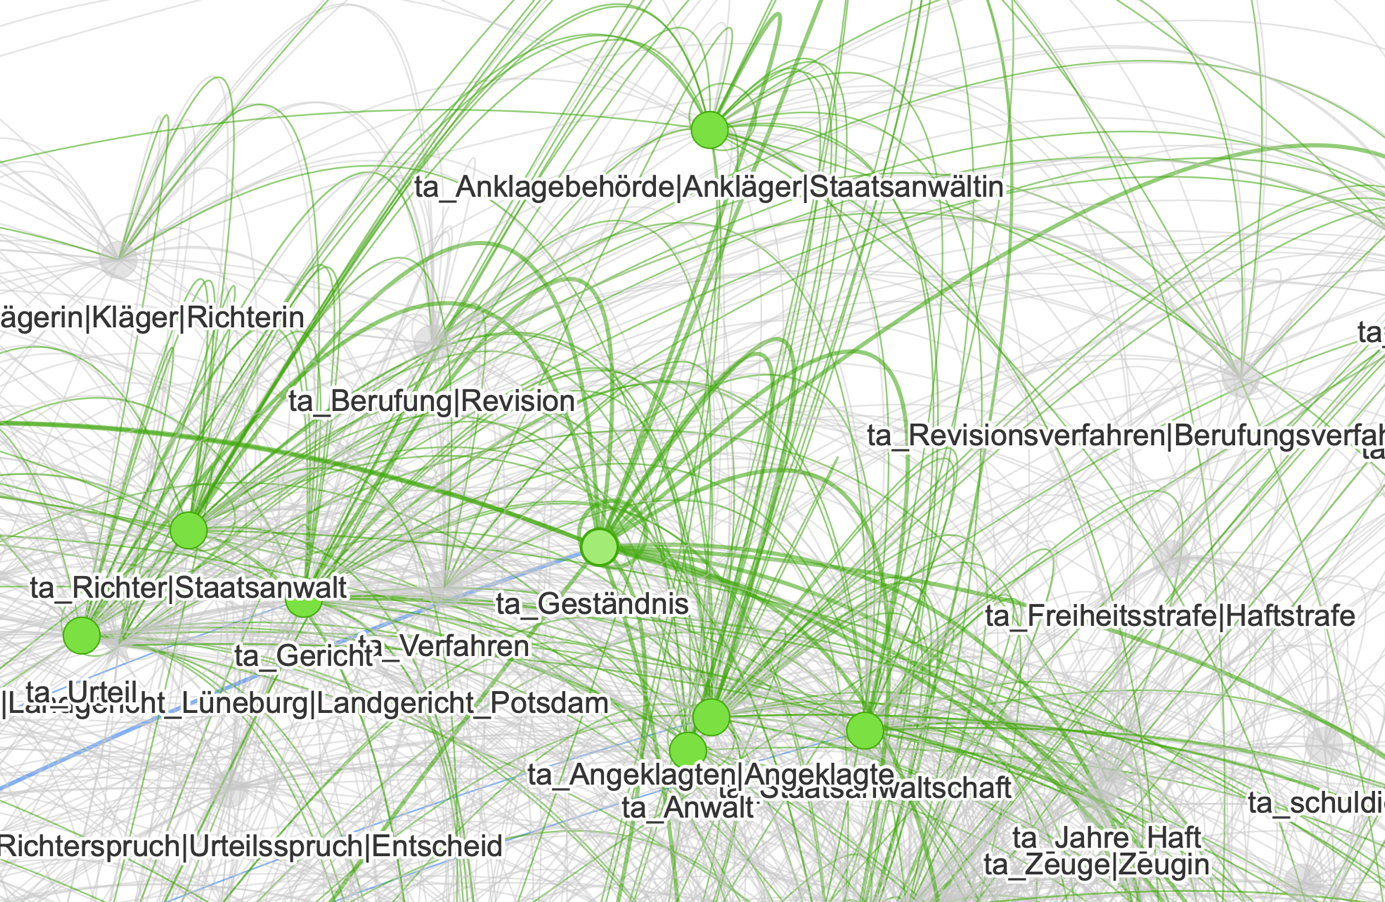
\includegraphics[width=\textwidth]{figures/media/image24.png}
  \caption{\label{fig:straftaten-beispiel}Ausschnitt aus dem thematischen Teil-Frame ‚Straftaten \& Juristisches` am Beispiel des Clusters \cluster{ta\_Geständnis}.}
\end{figure}

Im thematischen Teil-Frame ‚Straftaten \& Juristisches` (\figref{fig:straftaten-beispiel}) finden sich u.\,a. einzelne Straftaten (z.\,B. \cluster{05\_Gewalttaten{\breakbar}Straftaten{\breakbar}Morde}, \cluster{14\_Verbrechen}, \cluster{14\_Diebstähle{\breakbar}Körperverletzungen{\breakbar}Sachbeschädigungen}, \cluster{sp\_Sexualstraftaten{\breakbar}Körperverletzungen{\breakbar}Sexualdelikte}), gerichtliche und institutionelle Akteure der Strafverfolgung bzw. Ermittlungsbehörden (\cluster{02\_Staatsanwaltschaft}, \cluster{14\_Gerichtshof{\breakbar}Bundesgericht{\breakbar}Berufungsgericht}, \cluster{14\_Verteidiger{\breakbar}Verteidigung}, \cluster{14\_NSA{\breakbar}Bnd, sp\_schuldig\_gesprochen{\breakbar}zum\_Tode\_verurteilt{\breakbar}freigesprochen}) und einzelne Angeklagte (\cluster{08\_Ankläger{\breakbar}Kachelmann{\breakbar}Staatsanwältin}, \cluster{14\_Beate\_Zschäpe{\breakbar}Zschäpe{\breakbar}Nsu-prozess}, \cluster{we\_Mollath{\breakbar}seinen\_Mandanten{\breakbar}Gäfgen}).

Eine weitere in allen Subkorpora emergierende Netzwerk-Community (\figref{fig:staat-beispiel}) ist thematisch etwas vager, aber insofern äußerst relevant für den Extremismusdiskurs, als sie die FdGO, also die definitorische Antithese zum Extremismus, widerspiegelt.

\begin{figure}
  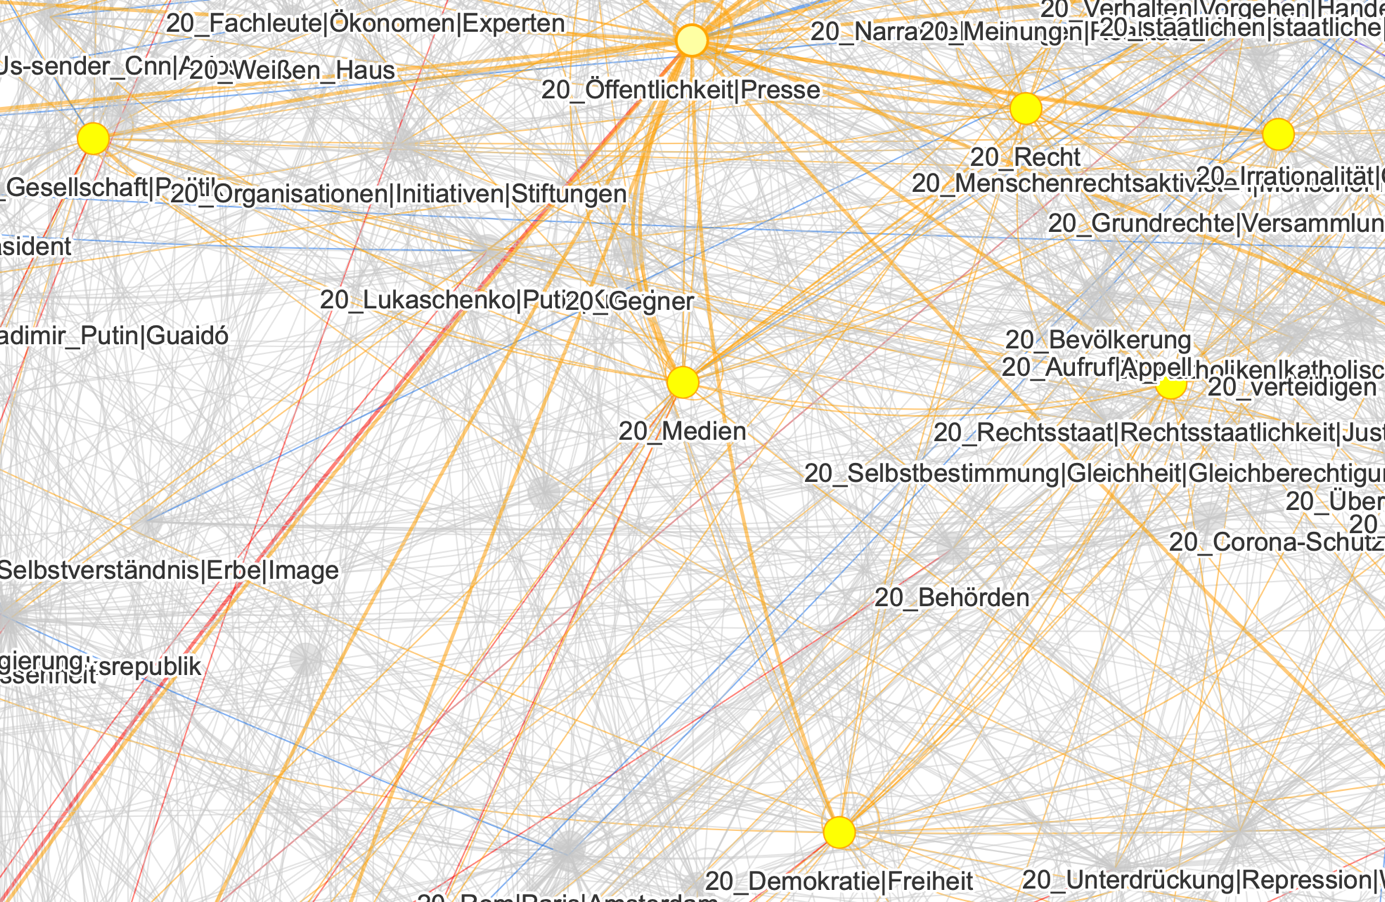
\includegraphics[width=\textwidth]{figures/media/image25.png}
  \caption{\label{fig:staat-beispiel}Ausschnitt aus dem thematischen Teil-Frame ‚Staat, FdGO \& Gesellschaft` am Beispiel des Clusters \cluster{20\_Öffentlichkeit{\breakbar}Presse}.}
\end{figure}

Hier sind FE gebündelt, die Grundrechte (\cluster{99\_Grundreche{\breakbar}Meinungsfreiheit{\breakbar}Menschenwürde}, \cluster{08\_Schutz}, \cluster{14\_Chancengleichheit{\breakbar}Selbstbestimmung{\breakbar}Gleichberechtigung}, \cluster{14\_Menschenwürde{\breakbar}Religionsfreiheit{\breakbar}Freiheitsrechte}), einzelne Werte (\cluster{05\_Ehre}, \cluster{14\_Solidarität}, \cluster{14\_Ideale{\breakbar}Ideologie{\breakbar}Überzeugungen}, \cluster{ta\_Toleranz}), die Organisation von Staat und Gesellschaft (\cluster{11\_Republik}, \cluster{14\_Gesellschaft}, \cluster{14\_Bundesrepublik}, \cluster{ta\_Staates}), gesellschaftliche Gruppen (\cluster{02\_Bürger}, \cluster{14\_Lesben{\breakbar}Schwule{\breakbar}Schwulen}, \cluster{14\_Elite{\breakbar}Eliten{\breakbar}Mittelschicht}, \cluster{14\_Religion} ), aber auch Aushandlungsprozesse und Bedrohungen ebendieser Ordnung (\cluster{02\_Kampf\_gegen}, \cluster{14\_Debatte{\breakbar}Diskussion}, \cluster{14\_verteidigen}, \cluster{14\_diskreditieren{\breakbar}provozieren{\breakbar}instrumentalisieren}, \cluster{20\_bedroht{\breakbar}gefährdet}, \cluster{20\_Antisemitismus{\breakbar}Rassismus{\breakbar}Rechtsextremismus}) widerspiegeln. Auch einschneidende negative historische Ereignisse bzw. Gräueltaten sind in diesem Cluster häufig enthalten (\cluster{14\_Barbarei{\breakbar}Grausamkeit{\breakbar}Brutalität}, \cluster{14\_Zweiten\_Weltkrieg{\breakbar}Ersten\_Weltkrieg}, \cluster{14\_Völkermord{\breakbar}Genozid{\breakbar}Armenien}). Dass diese besonders schweren historischen Verbrechen regelmäßig in diesem Netzwerk-Cluster enthalten sind, macht einen deutlichen Unterschied im Framing im Vergleich zu den zeitgenössischen Kriegen deutlich: Sie werden medial nicht in erster Linie als kriegerische Handlungen thematisiert, bei denen an bestimmten Orten mithilfe einzelner Waffen Angriffe verübt wurden, sondern insbesondere in ihrer historisch-gesellschaftlichen Bedeutung.

\begin{figure}
  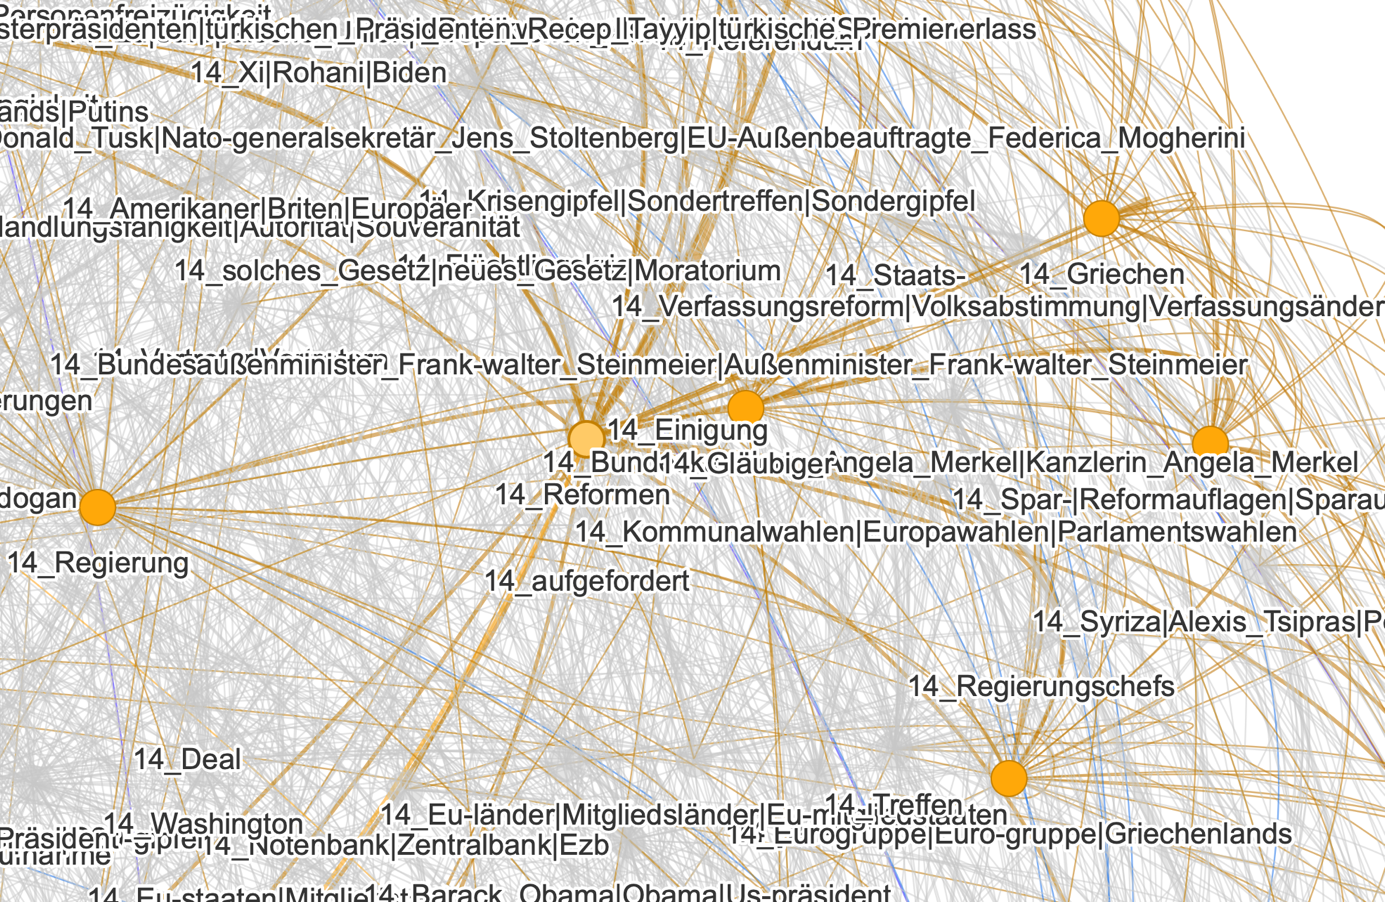
\includegraphics[width=\textwidth]{figures/media/image26.png}
  \caption{\label{fig:aussenpolitik-beispiel}Ausschnitt aus dem thematischen Teil-Frame ‚Außenpolitik` am Beispiel des Clusters \cluster{14\_Reformen}.}
\end{figure}

\begin{figure}
  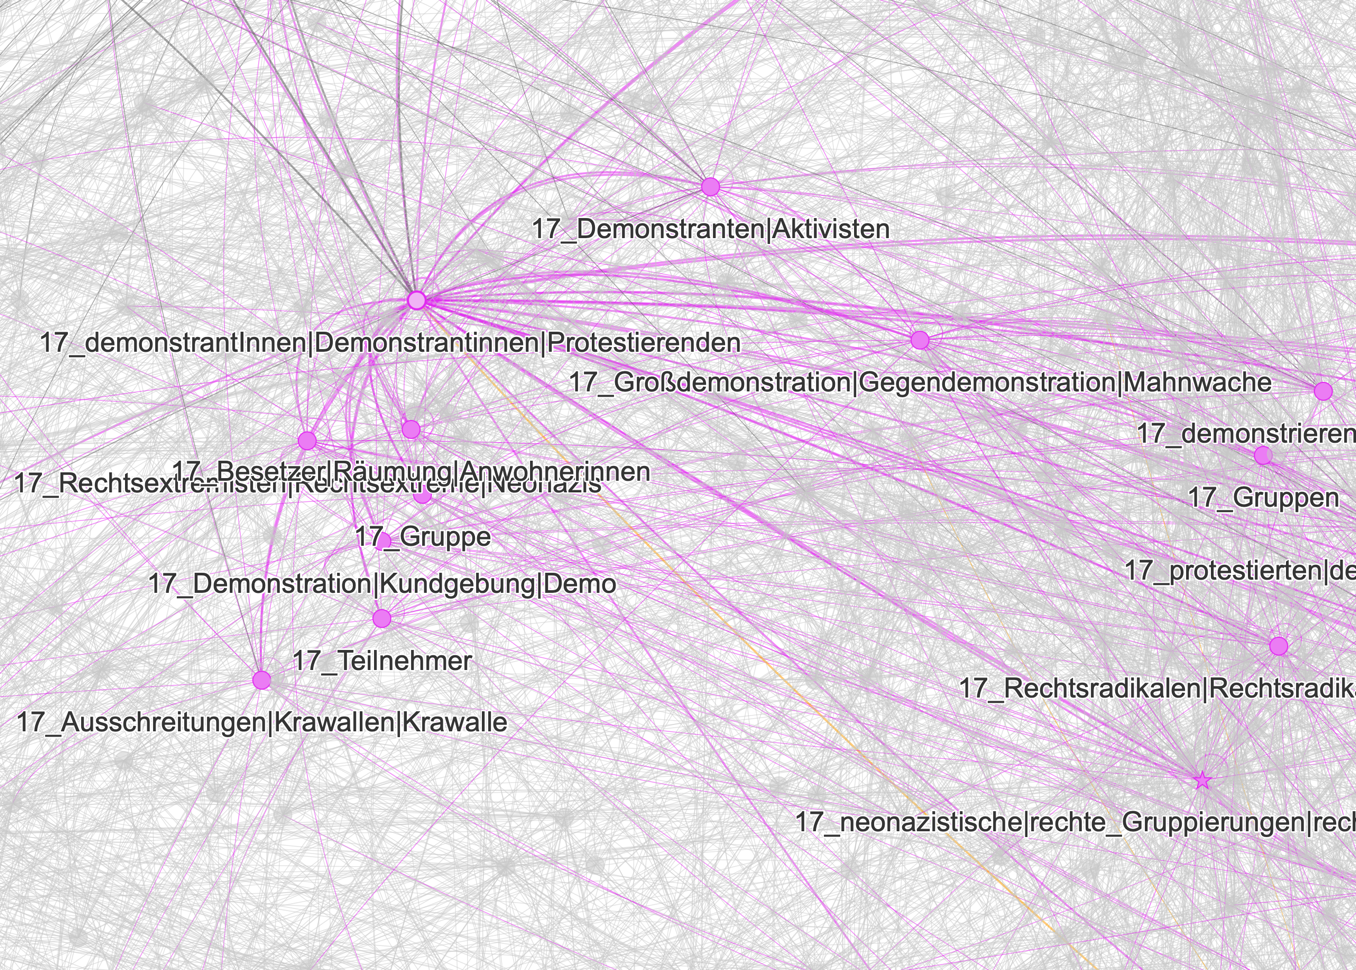
\includegraphics[width=\textwidth]{figures/media/image27.png}
  \caption{\label{fig:demonstrationen-beispiel}Ausschnitt aus dem thematischen Teil-Frame ‚Demonstrationen \& politischer Extremismus` am Beispiel des Clusters 17\cluster{\_demonstrantInnen{\breakbar}Demonstrantinnen{\breakbar}Protestierenden}.}
\end{figure}

Neben diesen vier in jedem Teilkorpus zu Tage tretenden Communities finden sich zwei weitere Cluster, die zwar nicht in allen, aber in den meisten der Subkorpora identifiziert wurden. So tritt die Community ‚Außenpolitik` (\figref{fig:aussenpolitik-beispiel}) in den Subkorpora 2002--2004, 2005--2007, 2008--2010, 2011--2013, 2014--2016 und \textsc{Spiegel} auf und die Community ‚Demonstrationen \& politischer Extremismus` in den Subkorpora 2002--2004, 2005--2007, 2008--2010, 2014--2016, 2017--2019, \textsc{Taz} und \textsc{Welt}. Im Cluster Außenpolitik finden sich internationale Akteure und Orte (\cluster{05\_Uno{\breakbar}Vereinten\_Nationen{\breakbar}UN}, \cluster{05\_Entwicklungsländer{\breakbar}Industriestaaten{\breakbar}Industrieländer}, \cluster{05\_Außenminister{\breakbar}Regierungschefs{\breakbar}Botschafter}, \cluster{05\_Europa{\breakbar}Deutschland{\breakbar}Amerika}, \cluster{11\_Notenbank{\breakbar}Zentralbank{\breakbar}Bundesbank,} \cluster{sp\_Burma{\breakbar}Myanmar{\breakbar}Simbabwe}), Praktiken (\cluster{05\_Gipfels{\breakbar}Treffens{\breakbar}G-8-Gipfels}, \cluster{05\_Scheitern}, \cluster{05\_Versprechen, 11\_Notkredite{\breakbar}Hilfskredite{\breakbar}Rettungsfonds}) sowie außenpolitische und diplomatische Projekte (\cluster{05\_Beitritt{\breakbar}Eu-beitritt}, \cluster{14\_Reformen}). Die Community ‚Demonstrationen \& politischer Extremismus` (\figref{fig:demonstrationen-beispiel}) umfasst Akteure, die an Demonstrationen teilnehmen (\cluster{05\_Gewerkschaften, 17\_Demonstranten{\breakbar}Aktivisten}), Akteure des Rechts- und Linksextremismus (\cluster{17\_Rechtsextremisten{\breakbar}Rechtsextreme{\breakbar}Neonazis}, \cluster{17\_Besetzer{\breakbar}Räumung{\breakbar}Anwohnerinnen}, \cluster{ta\_Antifas{\breakbar}Skins{\breakbar}Antifaschisten}) sowie Attribuierungen zu Demonstrationen (\cluster{ta\_friedlich}, \cluster{ta\_Ausschreitungen{\breakbar}Krawalle{\breakbar}Krawallen}, \cluster{we\_gewalttätigen\_Auseinandersetzungen{\breakbar}Straßenschlachten{\breakbar}gewaltsamen\_Auseinandersetzungen}).

\begin{figure}
  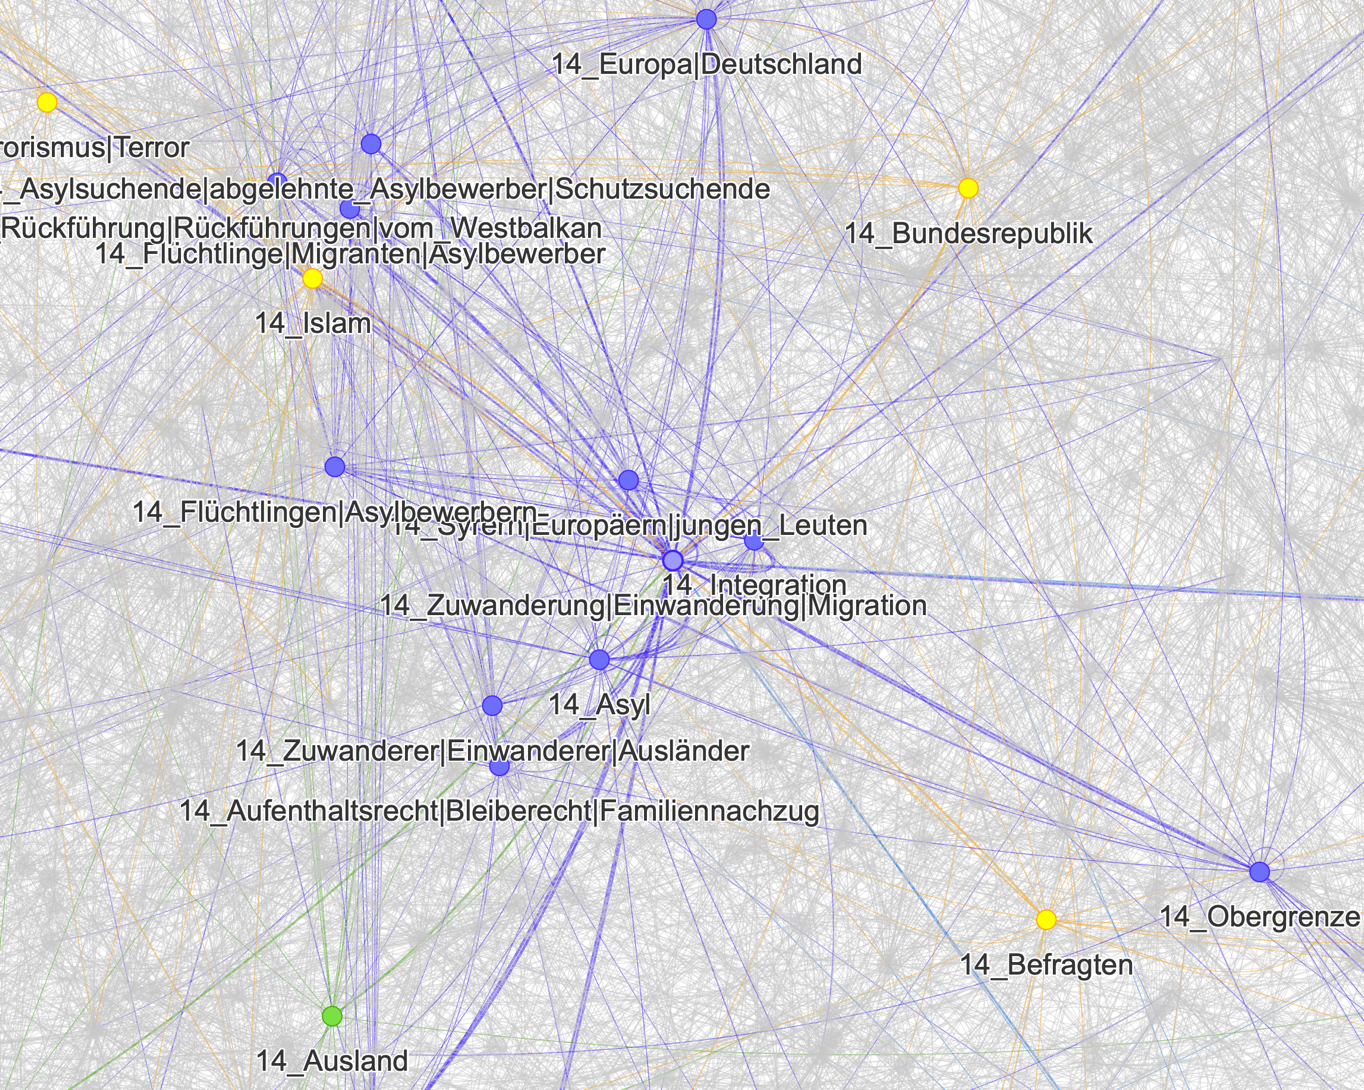
\includegraphics[width=\textwidth]{figures/media/image28.png}
  \caption{\label{fig:flucht-beispiel}Ausschnitt aus dem thematischen Teil-Frame ‚Flucht \& Migration` am Beispiel des Clusters 14\cluster{\_Zuwanderung{\breakbar}Einwanderung{\breakbar}Migration}.}
\end{figure}

Letztlich finden sich einige weitere Cluster, die nur in einzelnen Teilkorpora oder auch nur einmalig identifiziert werden. Dies betrifft das Cluster ‚Migration \& Flucht` (\figref{fig:flucht-beispiel}) in den Subkorpora 2014--2016, 2017--2019, \textsc{Taz} und \textsc{Welt} (\cluster{we\_Asylverfahren{\breakbar}Asylanträge}, \cluster{14\_Zuwanderer{\breakbar}Einwanderer{\breakbar}Ausländer}), ‚Geheimdienste` im \textsc{Welt}-Teilkorpus (\cluster{we\_Bnd{\breakbar}NSA}, \cluster{we\_Telefonaten{\breakbar}Anrufen{\breakbar}Kontakten}), ‚Unglücke, Attentate \& Gedenken` in den Subkorpora 2014--2016, 2017--2019, 2020--2021 und \textsc{Spiegel} (\cluster{14\_Lastwagen{\breakbar}LKW}, \cluster{17\_Attentäter}, \cluster{20\_Hanau}, \cluster{sp\_Unglück}), ‚Religion` im \textsc{Taz}-Subkorpus (\cluster{ta\_Gemeinschaft}, \cluster{ta\_Gläubige{\breakbar}Gläubigen{\breakbar}Pilger}) sowie ‚Nationalsozialismus \& DDR` im \textsc{Spiegel}-Teilkorpus (\cluster{sp\_Ddr}, \cluster{sp\_Nationalsozialisten{\breakbar}Nazis{\breakbar}Nationalsozialismus}). In zwei Fällen wurden auch Communities algorithmisch identifiziert, die jeweils nur ein Cluster umfassen (\cluster{99\_Anhänger{\breakbar}Gegner} und \cluster{02\_Erklärung}) und daher nicht weiter berücksichtigt wurden.

\section{Mesostruktur: Extremismusvarianten-Frames}\label{mesostruktur-extremismusvarianten-frames}

\subsection{Der Zeitraum 1999--2001}\label{der-zeitraum-1999-2001}

\subsubsection{\texorpdfstring{\emph{Corpus-driven} Voranalyse: Cluster mit hoher Cosinus-Distanz im Vergleich zum Gesamtkorpus}{Corpus-driven Voranalyse: Cluster mit hoher Cosinus-Distanz im Vergleich zum Gesamtkorpus}}\label{corpus-driven-voranalyse-cluster-mit-hoher-cosinus-distanz-im-vergleich-zum-gesamtkorpus}

Da der Zeitraum 1999--2001 das in diachroner Perspektive erste Teilkorpus darstellt, können an dieser Stelle keine semantischen Äquivalenzen von Clustern oder Verschiebungen im Vergleich zu einem vorhergehenden Zeitraum berichtet werden (siehe zu den quantitativen Voranalysen \chapref{vorgehen-und-zielsetzung}). Behelfsweise werden daher die Cluster-Distanzen zum auf dem Gesamtkorpus trainierten Word-Embedding-Modell (dem \emph{compass}) berechnet. Die Top 20 so ermittelten Cluster sind in \tabref{tab:cluster-high-cosine-distance-1999} dargestellt. Es zeichnen sich in der Liste der Cluster insbesondere im Bereich der Außenpolitik wesentliche Veränderungen ab. Cluster wie \cluster{99\_Al\_Gore{\breakbar}Gore{\breakbar}George\_W\_Bush} und \cluster{99\_Vizepräsident\_Al\_Gore{\breakbar}Mccain{\breakbar}John\_Mccain} weisen zum einen auf die US-amerikanische Präsidentschaftswahl des Jahres 2000 hin, zum anderen mit \cluster{99\_Irak} auch auf die im Anschluss an 9/11 geführten Debatten um die Rolle des Iraks bei den Anschlägen. Auch der Nahostkonflikt (\cluster{99\_Gaza-streifen{\breakbar}Westjordanland{\breakbar}Gazastreifen, 99\_ Ehud\_Barak{\breakbar}Ariel\_Scharon{\breakbar}Jassir\_Arafat}), außerparlamentarischer Protest (\cluster{99\_Neckarwestheim{\breakbar}Philippsburg{\breakbar}Atomtransporte}), kontroverse politisch-gesellschaftliche Debatten (\cluster{99\_Homo-ehe{\breakbar}Unterschriftensammlung{\breakbar}doppelte\_Staatsbürgerschaft}) sowie die CDU-Spendengeldaffäre \cluster{(99\_Weyrauch{\breakbar}Walther\_Leisler\_Kiep{\breakbar}Horst\_Weyrauch)} klingen an.

\begin{table}[t]\small
\caption{Cluster mit hoher Cosinus-Distanz im Vergleich zum Gesamtkorpus.}
\label{tab:cluster-high-cosine-distance-1999}
\begin{tabularx}{\textwidth}{X r}
\lsptoprule
Cluster & Cos.-Dist. \\
\midrule
\cluster{Al\_Gore{\breakbar}Gore{\breakbar}George\_W\_Bush} & 0.28 \\
\cluster{Spd-generalsekretär\_Franz\_Müntefering{\breakbar}Struck{\breakbar}CDU-Generalsekretärin\_Angela\_Merkel} & 0.26 \\
\cluster{Rühe{\breakbar}Möllemann{\breakbar}Wolfgang\_Schäuble} & 0.25 \\
\cluster{Vizepräsident\_Al\_Gore{\breakbar}Mccain{\breakbar}John\_Mccain} & 0.25 \\
\cluster{Neckarwestheim{\breakbar}Philippsburg{\breakbar}Atomtransporte} & 0.24 \\
\cluster{Weyrauch{\breakbar}Walther\_Leisler\_Kiep{\breakbar}Horst\_Weyrauch} & 0.24 \\
\cluster{Afp{\breakbar}ap{\breakbar}rtr} & 0.24 \\
\cluster{Ausnahmeregelung{\breakbar}Gesetzesänderung{\breakbar}Sonderregelung} & 0.24 \\
\cluster{rebellieren{\breakbar}ankämpfen{\breakbar}Parteiengesetz\_verstoßen} & 0.24 \\
\cluster{Irak} & 0.23 \\
\cluster{Ehud\_Barak{\breakbar}Ariel\_Scharon{\breakbar}Jassir\_Arafat} & 0.23 \\
\cluster{Jospin{\breakbar}Blair{\breakbar}Tony\_Blair} & 0.23 \\
\cluster{rot-grüne\_Koalition{\breakbar}Rot-grün{\breakbar}rot-grüne\_Regierung} & 0.22 \\
\cluster{Gipfel{\breakbar}Gipfeltreffen{\breakbar}Eu-gipfel} & 0.22 \\
\cluster{Verbrecher{\breakbar}Drogenhändler{\breakbar}Mafiosi} & 0.22 \\
\cluster{Oberlandesgericht{\breakbar}Olg{\breakbar}Bundesgerichtshof\_Bgh} & 0.22 \\
\cluster{Gaza-streifen{\breakbar}Westjordanland{\breakbar}Gazastreifen} & 0.22 \\
\cluster{Homo-ehe{\breakbar}Unterschriftensammlung{\breakbar}doppelte\_Staatsbürgerschaft} & 0.21 \\
\cluster{Kurden} & 0.21 \\
\cluster{europäischen\_Union\_Eu{\breakbar}europäische\_Union{\breakbar}Wto} & 0.21 \\
\lspbottomrule
\end{tabularx}
\end{table}

\subsubsection{Rechts- und Linksextremismus}\label{rechts--und-linksextremismus}

Es lassen sich in diesem Teilkorpus insbesondere die folgenden Cluster ausmachen, die auf Basis von Diskurswissen mit recht großer Sicherheit als Bestandteile eines Rechtsextremismus-Frames zu lesen sind: \cluster{99\_Neonazis{\breakbar}Skinheads{\breakbar}Rechtsextremisten (rechtsextreme Akteure und Akteure bei Demonstrationen)}, \cluster{99\_NPD}, \cluster{99\_Nazis}, \cluster{99\_Holocaust{\breakbar}Nationalsozialismus}, \cluster{99\_Fremdenfeindlichkeit{\breakbar}Ausländerfeindlichkeit{\breakbar}Rassismus (Charakteristika des Rechtsextremismus)}. Ein Problem für korpuslinguistische Verfahren, die auf Types beruhen, stellen homonyme oder polyseme Wörter dar (siehe \chapref{moegliche-fallstricke-bei-der-interpretation}). Dies betrifft in diesem Zeitraum das Cluster \cluster{99\_Republikaner{\breakbar}Demokraten}, dessen Wörter sich gut in einem Cluster zusammenfassen lassen, wenn sie auf die beiden US-amerikanischen Parteien referieren. Zugleich sind die Republikaner jedoch auch eine Partei des äußeren rechten Spektrums in Deutschland. Dieser Unterschied wird bei der Berechnung der Word Embeddings bzw. Cluster sowie der Kollokationen ebendieser nicht berücksichtigt. Mithin fließen beide Bedeutungen in die Positionierung des Clusters im Graphen ein und es weist einerseits Verbindungen zu Clustern wie \cluster{99\_Senat} oder \cluster{99\_Clinton{\breakbar}Bush{\breakbar}Putin} auf, andererseits auch zu \cluster{99\_Npd} und \cluster{99\_Kommunalwahlen{\breakbar}Europawahl{\breakbar}Europawahlen}.

Wählt man alle identifizierten Cluster im Graphen aus, lässt sich der Recht\-sextremismus-Frame dieses Zeitraumes (siehe \figref{fig:rechtsextremismus-frame-1999-2001} in \chapref{kollokation-von-word-embedding-clustern-als-frame-relationen-und-perspektivierung-kollokationsnetzwerke-als-frames}) visualisieren und die jeweilige Perspektivierungsleistung der einzelnen FE erschließen, indem die angeschlossenen FE -- unter Berücksichtigung ihrer Verortung in den thematischen Teil-Frames -- betrachtet werden. An den Akteur-Clustern \cluster{99\_Neonazis{\breakbar}Skinheads{\breakbar}Rechtsextremisten}, \cluster{99\_NPD} und \cluster{99\_Nazis} wird -- wie in \chapref{kollokation-von-word-embedding-clustern-als-frame-relationen-und-perspektivierung-kollokationsnetzwerke-als-frames} bereits umrissen -- deutlich, dass sie zwar alle Akteure des Rechtsextremismus enthalten, jedoch deutlich unterschiedliche Perspektivierungsleistungen erbringen.

\begin{figure}[t]
  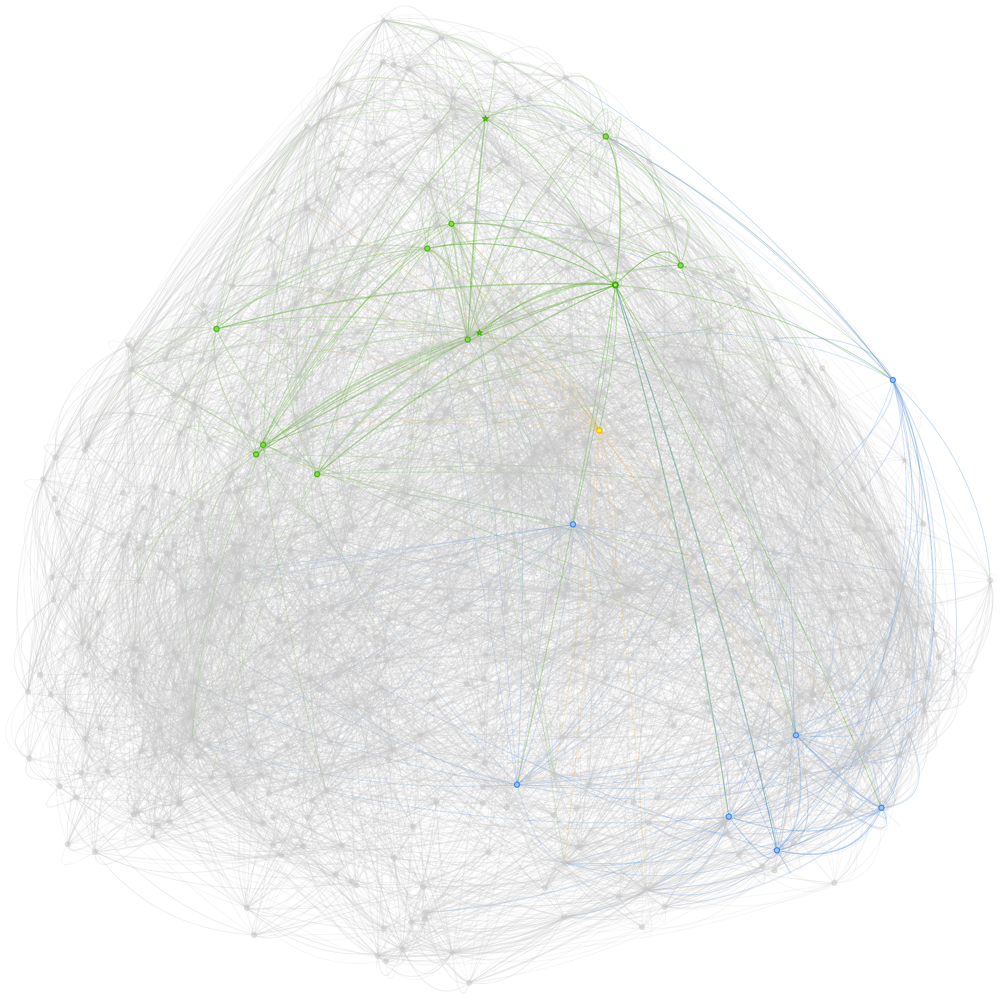
\includegraphics[width=.8\textwidth]{figures/media/image29.png}
  \caption{\label{fig:npd-frame}Thematische Verankerung des NPD-Frames.}
\end{figure}

So sind an das NPD-FE, das im juristischen Netzwerk-Cluster liegt, fast ausschließlich FE aus den Bereichen ‚Politik` und ‚Straftaten \& Juristisches` angeschlossen (siehe \figref{fig:npd-frame}). Durch den Anschluss an ersteren Bereich und FE wie \cluster{99\_Mitglieder}, \cluster{99\_Partei}, \cluster{99\_Antrag} wird die NPD als politische Partei geframet. Die Vernetzung in zweiterem Bereich macht hingegen den Status der NPD als rechtsextreme Partei deutlich. Zum einen finden sich hier die Cluster \cluster{99\_Verbot} und \cluster{99\_Bundesgerichtshof{\breakbar}Bgh{\breakbar}Bundesverfassungsgericht}, die das in diesem Zeitraum beginnende erste NPD-Verbotsverfahren zum Teil des verstehensrelevanten Wissens zum NPD- bzw. Rechtsextremismus-Frame machen; zum anderen Cluster wie \cluster{99\_Bnd{\breakbar}Fbi{\breakbar}Bka (Geheimdienste)}, \cluster{99\_Neonazis{\breakbar}Skinheads{\breakbar}Rechtsextremisten (rechtsextreme Akteure und Akteure bei Demonstrationen)}, \cluster{99\_Demonstrationen{\breakbar}Proteste{\breakbar}Protesten} oder \cluster{99\_Autonomen{\breakbar}Rechtsextremen{\breakbar}Aufmärsche (Demonstrationen des politischen Extremismus inkl. Akteuren, Demonstrationsformen, Charakteristika)}, die die Organisation von bzw. Beteiligung an Demonstrationen, Verflechtungen mit rechtsextremistischen Gruppen oder die Beobachtung durch den Verfassungsschutz abbilden.

\begin{figure}
  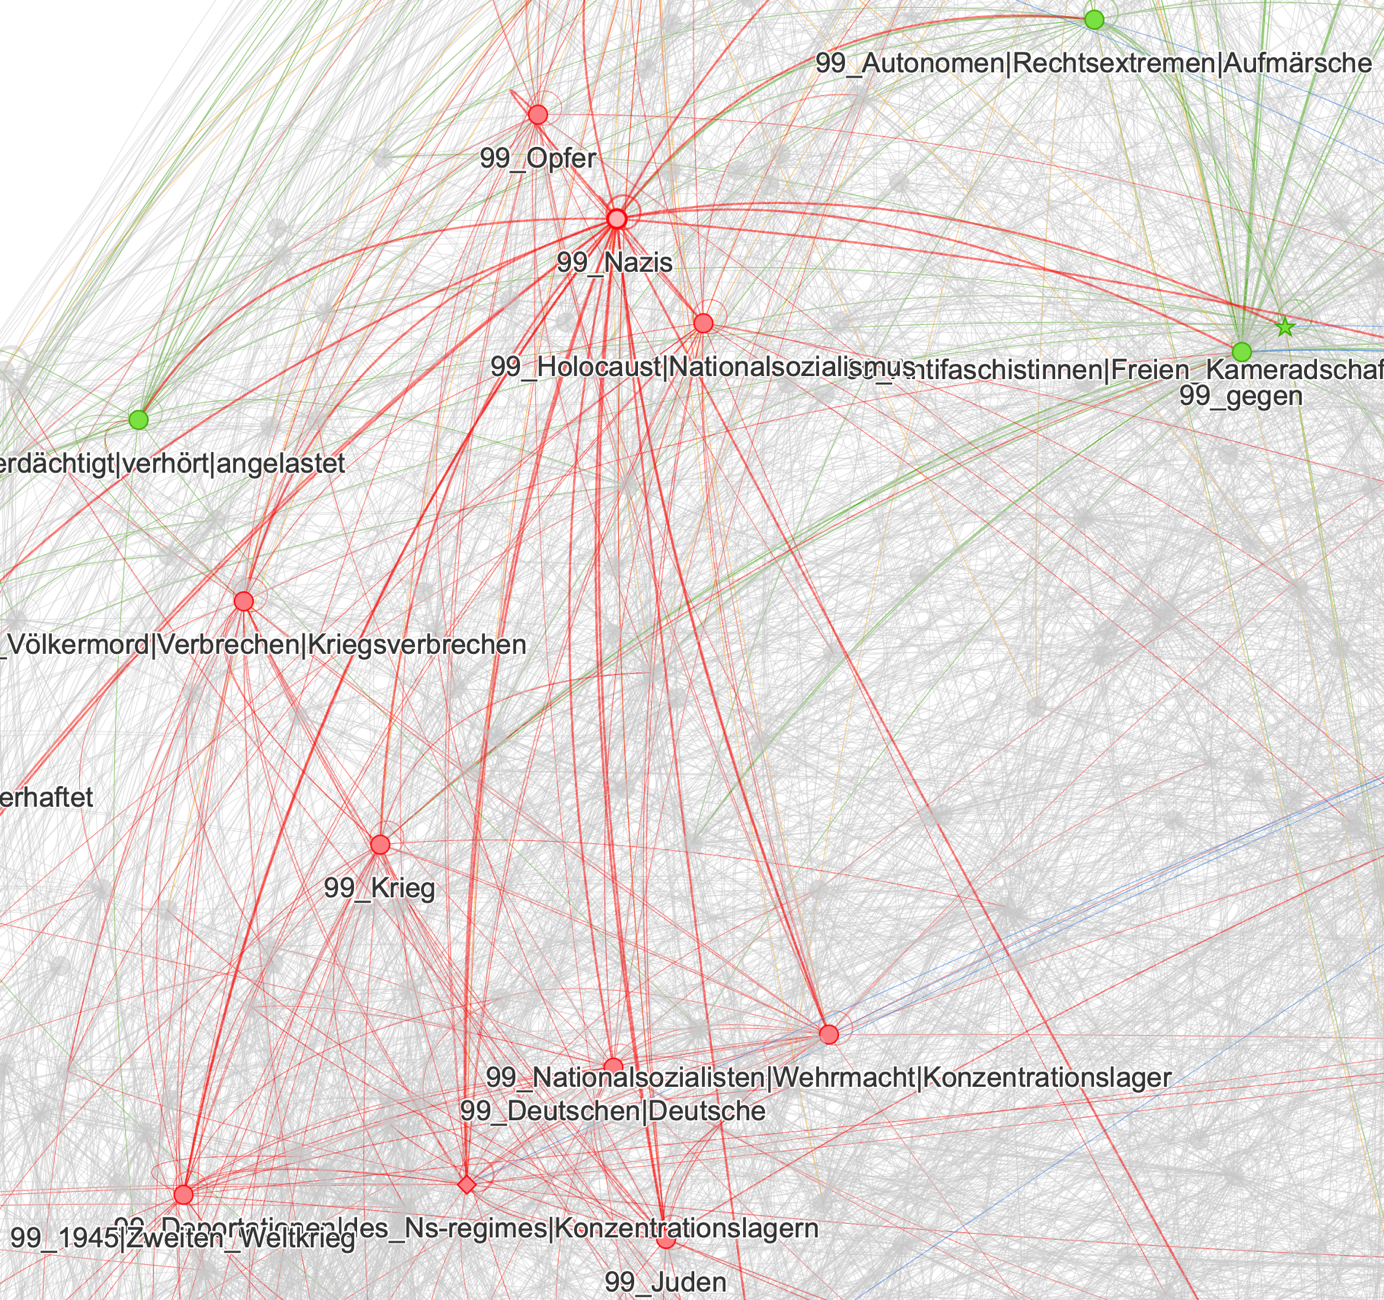
\includegraphics[width=\textwidth]{figures/media/image30.png}
  \caption{\label{fig:perspektivierung-nazis}Perspektivierung rechtsextremistischer Akteure durch das FE \cluster{99\_Nazis}.}
\end{figure}

Das Cluster \cluster{99\_Nazi} hingegen prägt deutlich andere Verbindungen im Frame aus (siehe \figref{fig:perspektivierung-nazis}). Es gehört zum thematischen Teil-Frame ‚Krieg \& Islamismus` und ist in diesem auch am meisten vernetzt, wobei fast alle hier angeschlossenen FE einen Bezug zur Zeit des Zweiten Weltkriegs aufweisen (u.\,a. \cluster{99\_Juden}, \cluster{99\_Krieg}, \cluster{99\_1945{\breakbar}Zweiten\_Weltkrieg}, \cluster{99\_Völkermord{\breakbar}Verbrechen{\breakbar}Kriegsverbrechen}). Es weist jedoch auch einzelne Verbindungen in die Cluster ‚Staat, FdGO \& Gesellschaft` (u.\,a. \cluster{99\_Fremdenfeindlichkeit{\breakbar}Ausländerfeindlichkeit{\breakbar}Rassismus}) und ‚Straftaten \& Jurstisches` (\cluster{99\_Autonomen{\breakbar}Rechtsextremen{\breakbar}Aufmärsche}) auf, die zeigen, dass der Ausdruck \emph{Nazis} mitunter auch in Zusammenhang mit zeitgenössischen Phänomenen des Rechtsextremismus genutzt wird, wenn auch deutlich seltener (siehe auch \chapref{kollokation-von-word-embedding-clustern-als-frame-relationen-und-perspektivierung-kollokationsnetzwerke-als-frames}).

\begin{figure}
  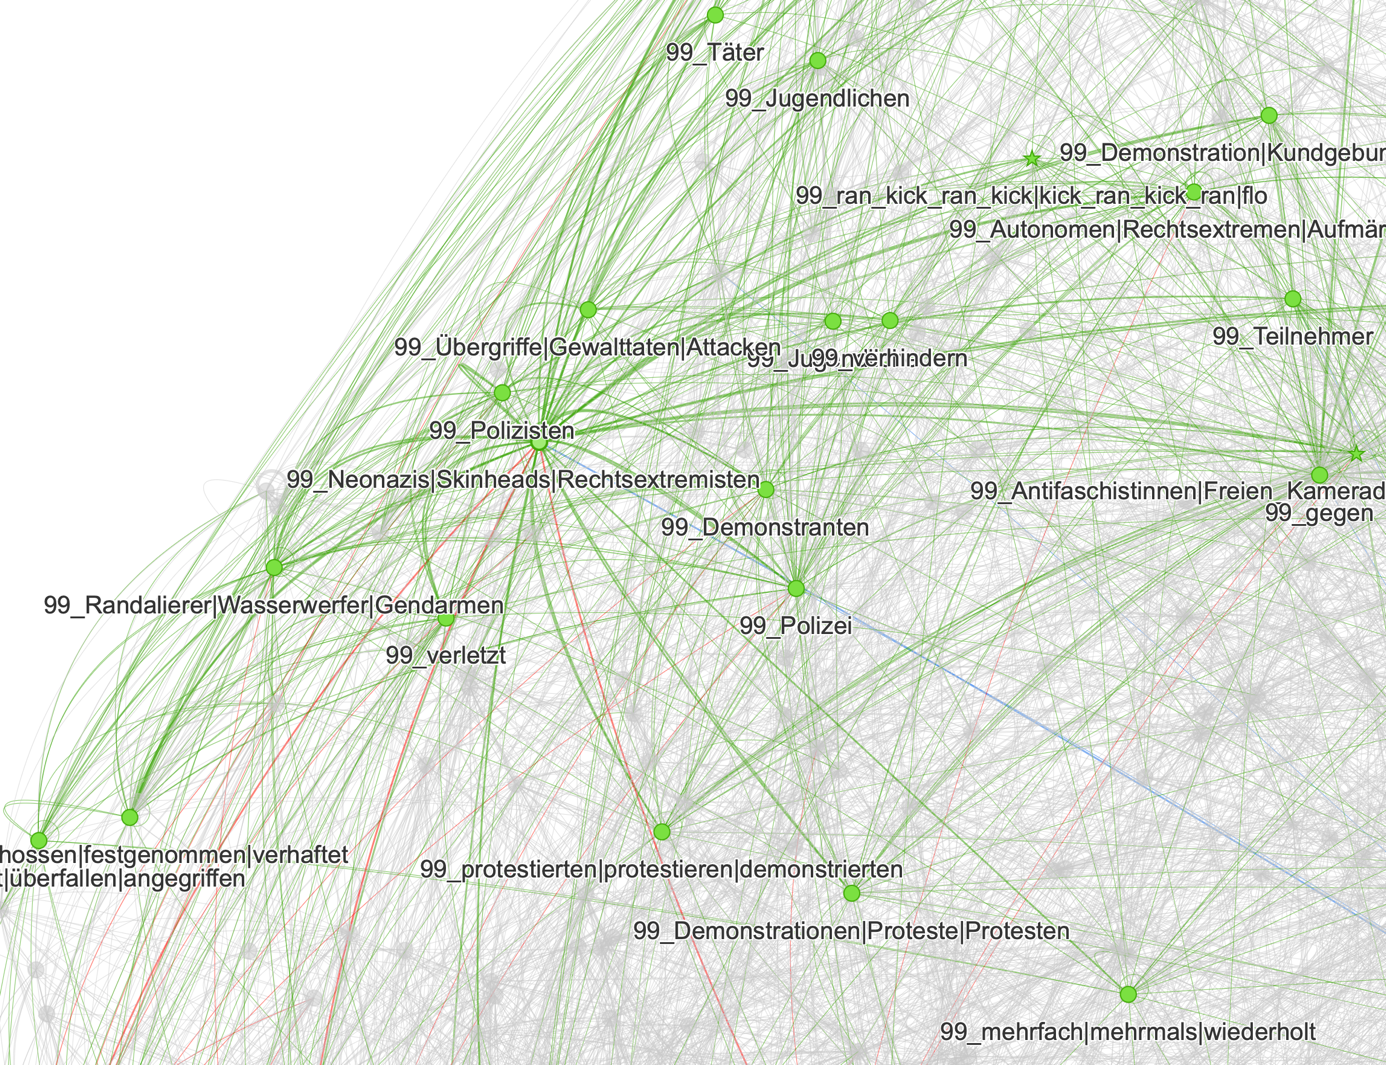
\includegraphics[width=\textwidth]{figures/media/image31.png}
  \caption{\label{fig:perspektivierung-neonazis}Perspektivierung rechtsextremistischer Akteure durch das FE \cluster{99\_Neonazis{\breakbar}Skinheads{\breakbar}Rechtsextremisten}.}
\end{figure}

Das Cluster \cluster{99\_Neonazis{\breakbar}Skinheads{\breakbar}Rechtsextremisten}, das außer den namensgebenden Wörtern auch die Ausdrücke \emph{Polizeisprecher}, \emph{Aktivisten}, \emph{Sicherheitskräfte}, \emph{Ausschreitungen}, \emph{nach\_Polizeiangaben}, \emph{Hooligans}, \emph{Polizeibeamte} und \emph{Festnahmen} umfasst, und insofern neben rechtsextremen Akteuren auch andere an Demonstrationen beteiligte Akteure sowie einzelne assoziierte Handlungen enthält, ist hingegen im Bereich des der ‚Straftaten \& des Juristischen` zu verorten (siehe \figref{fig:perspektivierung-neonazis}). Es zeigt sich dabei ein Framing, das insbesondere gewaltvolles Handeln (u.\,a. \cluster{99\_verletzt}, \cluster{99\_vergewaltigt{\breakbar}überfallen{\breakbar}angegriffen}, \cluster{99\_Übergriffe{\breakbar}Gewalttaten{\breakbar}Attacken}) und seine Verfolgung (u.\,a. \cluster{99\_Tat}, \cluster{99\_Täter}, \cluster{99\_Polizei}, \cluster{99\_Beamten{\breakbar}Beamte}) sowie Demonstrationen (u.\,a. \cluster{99\_Demonstranten}, \cluster{99\_demonstrationen{\breakbar}Proteste{\breakbar}Protesten}) und Organisiertheit (u.\,a. \cluster{99\_Teilnehmer}, \cluster{99\_Gruppe}, \cluster{99\_Autonomen{\breakbar}Rechtsextremen{\breakbar}Aufmärsche}) in den Vordergrund stellt. Dass etwa der syntagmatische Bezug zu Gewalt und Strafverfolgung der Wörter des Clusters nicht nur auf die enthaltenen Wörter wie \emph{Polizeibeamte} oder \emph{Festnahmen} zurückgeht, die ja auch außerhalb rechtsextremistischer Kontexte vorkommen können, lässt sich zeigen, indem (\emph{corpus-based}) die Kollokationen einzelner Wörter nachgeprüft werden. Das Wort \emph{Skinheads} etwa, das in diesem Zeitraum -- wie im Tooltipp zum Knoten ersichtlich -- in Bezug auf seine Keyness hochsignifikant (626,7 \emph{Log-Likelihood}) ist, hat unter seinen 50 Top-Kollokaten Wörter wie \emph{überfallen}, \emph{angepöbelt}, \emph{festgenommen}, \emph{Baseballschläger}, \emph{schlugen} oder \emph{Tode\_geprügelt}, was den Zusammenhang der rechtsextremen Akteure mit Gewalttaten und ihrer Ermittlung vereindeutigt.
\largerpage[-1]

\begin{figure}[t]
  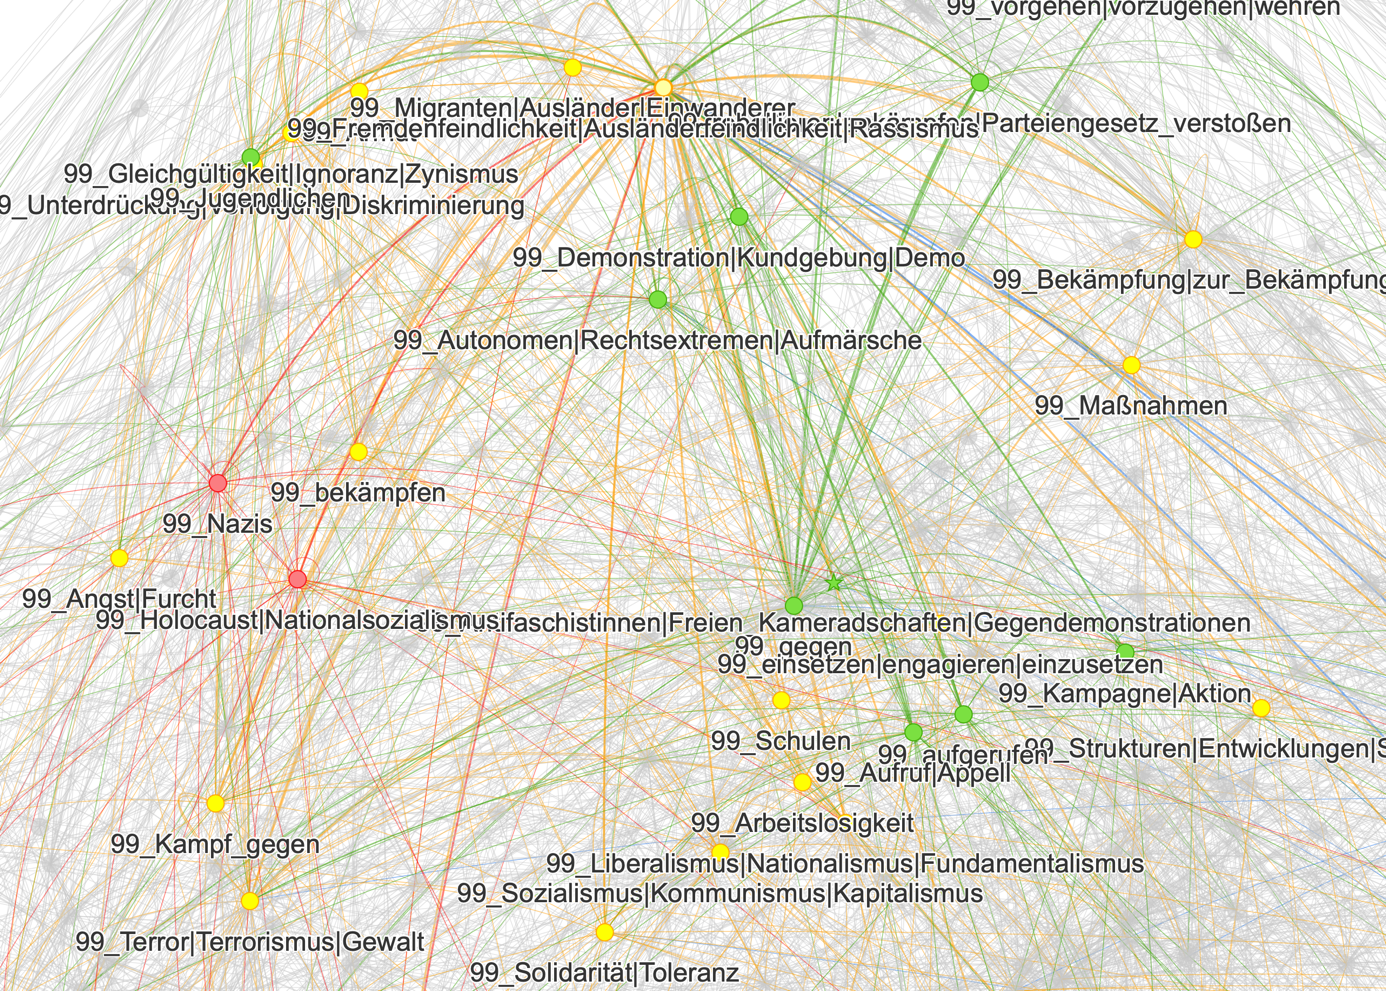
\includegraphics[width=\textwidth]{figures/media/image32.png}
  \caption{\label{fig:xenophobie-rassismus}Perspektivierung des Rechtsextremismus-Frames durch das FE \cluster{99\_Fremdenfeindlichkeit{\breakbar}Ausländerfeindlichkeit{\breakbar}Rassismus}.}
\end{figure}

Als letztes Cluster dieses Varianten-Frames soll das im thematischen Bereich ‚Staat, FdGO \& Gesellschaft` angesiedelte FE \cluster{99\_Fremdenfeindlichkeit{\breakbar}Ausländerfeindlichkeit{\breakbar}Rassismus (Charakteristika des Rechtsextremismus)} in den Blick genommen werden (\figref{fig:xenophobie-rassismus}). Wird dieses FE evoziert, treten erneut gänzlich andere Bedeutungsanteile des Rechtsextremismus-Frames in den Vordergrund. Angeschlossene FE wie \cluster{99\_Maßnahmen}, \cluster{99\_einsetzen{\breakbar}engagieren{\breakbar}einzusetzen}, \cluster{99\_Bekämpfung{\breakbar}zur\_Bekämpfung}, \cluster{99\_Mittel}, \cluster{99\_Kampf\_gegen} stellen Rechtsextremismus und seine Eigenschaften ein zu bekämpfendes Problem heraus. Es ist darüber hinaus mit anderen gesellschaftlichen Problemen wie \cluster{99\_Armut} oder \cluster{99\_Arbeitslosigkeit} verbunden, wobei eine Sichtung der entsprechenden Belegstellen zeigt, dass diese sowohl als Ursachen als auch als assoziierte kontige Konzepte zu lesen sind. Sie werden dabei oft in konjunktiv verknüpften Aufzählungen realisiert (siehe Belege K02--K04 in \tabref{tab:K02-K04}).

\begin{table}
  \caption{Konkordanzen zur Kollokation der Cluster \cluster{99\_Arbeitslosigkeit} und \cluster{99\_Fremdenfeindlichkeit{\breakbar}Ausländerfeindlichkeit{\breakbar}Rassismus}.}
  \label{tab:K02-K04}
K02 taz\_368196
\begin{tabularx}{\textwidth}{QQQ}
\toprule
noch private Niederlagen und Demütigungen wie die Scheidung von seiner Frau dazu dann Wende und & {[}\cluster{99\_Arbeitslosigkeit}: \textbf{Arbeitslosigkeit}{]}\newline
\textbf{und}\newline
{[}\cluster{99\_Fremdenfeindlichkeit{\breakbar}Ausländerfeindlichkeit{\breakbar}Rassismus:} \textbf{Ausländerfeindlichkeit}{]} & das volle\_Programm und im Mauerschützenprozess wird ausgerechnet sein inzwischen erwachsener Mannschaftskapitän angeklagt Heiko armer kleiner \\
\bottomrule
\end{tabularx}
\bigskip \newline
K03 taz\_92529
\begin{tabularx}{\textwidth}{QQQ}
\toprule
die innenpolitische\_Lage die Zuwanderung erwünscht oder unerwünscht macht bestenfalls heimlich und hinter\_vorgehaltener\_Hand diskutiert ich\_glaube dass & {[}\cluster{99\_Arbeitslosigkeit}: \textbf{Arbeitslosigkeit}{]}\newline
\textbf{und}\newline
{[}\cluster{99\_Fremdenfeindlichkeit{\breakbar}Ausländerfeindlichkeit{\breakbar}Rassismus:} \textbf{Ausländerfeindlichkeit}{]} & Argumente sein können den Ausländerzuzug zu drosseln braucht Deutschland ein Einwanderungsgesetz ja ich\_denke dass wir \\
\bottomrule
\end{tabularx}
\bigskip \newline
K04 welt\_26766
\begin{tabularx}{\textwidth}{QQQ}
\toprule
neuen Liberalismus der all\_jenen zugute\_kommen soll über die der Wirtschaftsboom der neunziger\_Jahre hinweggegangen ist dem & {[}\cluster{99\_Fremdenfeindlichkeit{\breakbar}Ausländerfeindlichkeit{\breakbar}Rassismus:} \textbf{Rassismus}{]}\newline
\textbf{und der}\newline
{[}\cluster{99\_Armut}: \textbf{Armut}{]} & in Amerika will er den Kampf\_ansagen und eine Krankenversicherung für alle Amerikaner schaffen große Aufgaben \\
\bottomrule
\end{tabularx}
\end{table}

Einige Cluster lassen sich weder eindeutig rechten noch linken extremistischen Bewegungen zuordnen und bilden so einen variantenübergreifenden Frame des politischen Extremismus. Der bereits skizzierte Rechtsextremismus-Frame kann im Sinne eines rekursiven Frame-Modells auch als Teil dieses Frames betrachtet werden. Einschlägig ist dabei insbesondere das Cluster \cluster{99\_Autonomen{\breakbar}Rechtsextremen{\breakbar}Aufmärsche (Politischer Extremismus \& Protest)}.\footnote{Ein weiteres Cluster \cluster{99\_Antifaschistinnen{\breakbar}Freien\_Kameradschaften{\breakbar}Gegendemonstrationen} erscheint zwar ebenfalls zu diesem Bereich gehörig -- und dies trifft auf eine Vielzahl der beinhalteten Wörter auch zu -- ist aber mit 254 enthaltenen Wörtern relativ groß und semantisch heterogen, sodass es nicht weiter ausgewertet wird.} Seine Relationen im Frame liegen größtenteils im thematischen Bereich ‚Straftaten \& Juristisches`, wo es ähnliche Verbindungen ausprägt wie das bereits besprochene Cluster \cluster{99\_Neonazis{\breakbar}Skinheads{\breakbar}Rechtsextremisten}, sodass Gewalt und Demonstrationen auch hier Teil des Framings sind. Die gewaltbezogenen FE unterscheiden sich jedoch insofern als besonders schwere Straftaten wie \cluster{99\_vergewaltigt{\breakbar}überfallen{\breakbar}angegriffen} hier nicht mehr assoziiert sind. Eine Sichtung der Konkordanzen zur Kookkurrenz mit dem Cluster \cluster{99\_Übergriffe{\breakbar}Gewalttaten{\breakbar}Attacken} wiederum macht deutlich, dass es dabei in der großen Mehrzahl um rechte Gewalt, oft gegen linke Akteure, geht. Es finden sich darüber hinaus Verbindungen in die Netzwerk-Community Politik mit FE wie \cluster{99\_Widerstand}, \cluster{99\_Vereine{\breakbar}Verbände{\breakbar}Vereinen} und in den Bereich ‚Staat, FdGO \& Gesellschaft` mit FE wie \cluster{99\_Organisationen{\breakbar}Initiativen{\breakbar}Institutionen} oder \cluster{99\_Bewegung}, die ebenfalls auf die Organisiertheit Bezug nehmen, jedoch dabei eine stärker legitimierende Perspektivierung andeuten als die äquivalenten FE im Rechtsextremismus-Frame.

\subsubsection{Islamismus}\label{islamismus}

Für den Islamismus-Frame erscheinen die folgenden FE besonders einschlägig, die alle im thematischen Teil-Frame ‚Krieg \& Islamismus` zu finden sind: \cluster{99\_Hebron{\breakbar}jüdische\_Siedler{\breakbar}israelischen\_Armee} \cluster{(Nahostkonflikt)}, \cluster{99\_Israelis{\breakbar}Palästinenser{\breakbar}Palästinensern (Bevölkerungsgruppen Nahostkonflikt)}, \cluster{99\_Islamisten{\breakbar}islamistischen{\breakbar}Pkk (extremistische Gruppierungen im Ausland, insb. Islamismus)}, \cluster{99\_Taliban}, \cluster{99\_Terroristen{\breakbar}Bin\_Laden{\breakbar}Waffen (Terroristen{\slash}Waffen)} und \cluster{Hussein{\breakbar}Abu{\breakbar}Ahmed} \cluster{(terroristische bzw. diktatorische Akteure)}.

Die beiden FE, die auf den Nahostkonflikt Bezug nehmen, werden durch angeschlossene Cluster wie u.\,a. \cluster{99\_getötet}, \cluster{99\_Bombe{\breakbar}Detonation{\breakbar}Sprengsatz (Attentate)}, \cluster{99\_verletzt\_worden} als gewaltvoller Konflikt geframet, der durch kriegerische Handlungen und Attentate geführt wird. FE aus dem Netzwerk-Cluster ‚Politik` wie \cluster{99\_Scharon{\breakbar}Barak{\breakbar}Arafat}, \cluster{99\_Besuch} und \cluster{99\_Gipfel{\breakbar}Gipfeltreffen{\breakbar}EU-gipfel} sowie aus dem Bereich ‚Staat, FdGO \& Gesellschaft` wie \cluster{99\_Umsetzung}, \cluster{99\_Verhandlungen{\breakbar}Gespräche} zeigen zudem die diplomatischen Bemühungen zur Lösung des Konfliktes an.

Die drei weiteren identifizierten FE und die an sie angeschlossenen FE tragen ebenfalls zu einem Framing von Islamismus bei, das durch kriegerische Handlungen und Attentate im Ausland markiert ist (\cluster{99\_Bombenangriffe{\breakbar}Bombardements{\breakbar}Bombardierungen}, \cluster{99\_Irak}, \cluster{99\_Nordkorea{\breakbar}Libyen{\breakbar}Syrien}) und bei dem nicht nur Staaten, sondern auch einzelne extremistische Gruppierungen eine Rolle spielen: \cluster{99\_Islamisten{\breakbar}islamistischen{\breakbar}Pkk} \cluster{(islamistische Akteure, aber auch Akteure des auslandsbezogenen Extremismus wie \emph{Eta} und \emph{Pkk})}, \cluster{99\_Rebellen}, \cluster{99\_Taliban} und weitere. Die Anschläge vom 11. September 2001 sind in diesem Zeitraum noch nicht deutlich im Frame sichtbar, was vermutlich darauf zurückgeht, dass sie erst gegen Ende dieses zeitlichen Abschnittes stattgefunden haben. Weitere epistemische Spezifizierungen finden sich in den anderen thematischen Frame-Teilen: Das Cluster ‚Staat, FdGO \& Gesellschaft` hebt einerseits den Aspekt der Zugehörigkeit, der im Islamismus-Frame durch Fragen der Religion und Herkunft eine besondere Rolle spielt, hervor (\cluster{99\_christlichen{\breakbar}religiösen{\breakbar}christliche}, \cluster{99\_Einheit{\breakbar}Nation{\breakbar}Gemeinschaft}, \cluster{99\_Identität{\breakbar}Herkunft}) und konstitutiert Islamismus andererseits als zu bekämpfendes Phänomen (\cluster{99\_Kampf\_gegen}, \cluster{99\_bekämpfen}). Im thematischen Teil-Frame ‚Politik` schlagen sich neben politischen Akteuren (u.\,a. \cluster{99\_Scharon{\breakbar}Barak{\breakbar}Arafat}, \cluster{99\_Präsident\_Bill\_Clinton{\breakbar}Bill\_Clinton{\breakbar}Us-präsident\_George\_W\_Bush}) auch Fragen der Anhängerschaft (u.\,a. \cluster{99\_Mitgliedern}, \cluster{99\_Anhänger{\breakbar}Gegner}, \cluster{99\_Vereine{\breakbar}Verbände{\breakbar}Vereinen}) nieder.

\subsubsection{Fazit}\label{fazit}

Insgesamt zeigen sich in diesem Zeitraum deutliche Unterschiede zwischen dem Framing von politischem Extremismus und Islamismus. Bei ersterem ist nur der Rechtsextremismus epistemisch ausdifferenziert im Frame angelegt. Es finden sich eigene Cluster zu Akteuren, dem Nationalsozialismus sowie zu Charakteristika dieser Extremismusform, wohingegen linksextreme Akteure oder Handlungen nur gemeinsam mit solchen des Rechtsextremismus in Clustern zusammengefasst vorkommen. Dies deutet an, dass Linksextremismus in diesem Zeitraum kein frequent thematisiertes oder deutlich divergent geframetes Phänomen darstellt, was sich damit deckt, dass in den entsprechenden Clustern Ausdrücke wie \emph{Rechtsextremismus} (1686 Vorkommen) oder \emph{Rechtsextremisten} (819 Vorkommen) um ein Vielfaches häufiger auftreten als etwa die jeweils 83 Mal vorkommenden Ausdrücke \emph{Linksextremismus} und \emph{Linksextremisten}. Dass sich auch bei mitunter geteilten Clustern dennoch ein eigener Rechtsextremismus-Frame abgrenzen lässt, zeigt, dass beide Extremismusvarianten zwar in Teilen ein ähnliches Framing, jedoch im Falle des Rechtsextremimus auch Alleinstellungsmerkmale aufweisen. Diese bestehen insbesondere im historischen Bezug der auf den Zweiten Weltkrieg verweisenden FE, dem FE der in einem Verbotsverfahren begriffenen NPD sowie den attributiven Zuschreibungen an Rechtsextremismus, die ebenfalls in einem FE organisiert sind. Als geteilte Merkmale des politischen Extremismus in diesem Zeitraum tritt insbesondere die Praktik des Demonstrierens und die Organisiertheit hervor. Letztere und auch die Assoziation mit Gewalt haben jedoch eine andere Qualität als im Rechtsextremismus-Frame und werden nicht gleichermaßen negativ perspektiviert.

Der Islamismus-Frame ist ebenfalls stark durch gewaltvolles Handeln geprägt. Dieses wird jedoch in Form von kriegerischen Handlungen und Attentaten realisiert, u.\,a. im Nahostkonflikt. Es finden sich hier einzelne FE, die auch Akteure des sogenannten auslandsbezogenen Extremismus abbilden wie die PKK oder ETA. Weiterhin finden sich auf Akteursebene politische Akteure wie Präsidenten der USA oder Israels und Terrororganisationen wie die Taliban.

\subsection{Der Zeitraum 2002--2004}\label{der-zeitraum-2002-2004}

\subsubsection{\texorpdfstring{\emph{Corpus-driven} Voranalyse: Thematisch gruppierte Auswahl semantisch äquivalenter Cluster im Vergleich zu den Kern-FE des vorigen Zeitraums}{Corpus-driven Voranalyse: Thematisch gruppierte Auswahl semantisch äquivalenter Cluster im Vergleich zu den Kern-FE des vorigen Zeitraums}}\label{corpus-driven-voranalyse-thematisch-gruppierte-auswahl-semantisch-aequivalenter-cluster-im-vergleich-zu-den-kern-fe-des-vorigen-zeitraums}

Um Kandidaten für die im Zeitraum 2002--2004 für den politischen Extremismus relevanten FE zu identifizieren, wurden zunächst die im Vektorraum in der Nähe der Cluster des vorigen Zeitraums befindlichen Cluster ermittelt. Tabelle 3 im Anhang zeigt pro Cluster des Zeitraumes 1999--2001 die fünf Cluster im Zeitraum 2002--2004 mit der höchsten Cosinus-Ähnlichkeit. Die Ergebnisse zeigen, dass einige FE des Zeitraumes 1999--2001 sehr äquivalente FE mit teils großen lexikalischen Überlappungen im Folgezeitraum aufweisen, was durch hohe Cosinus-Ähnlichkeitswerte von 0,85 und höher quantitativ unterlegt ist. Beispiele hierfür sind die Äquivalenzen \cluster{99\_NPD} zu \cluster{02\_NPD (0.91)}, \cluster{99\_Holocaust{\breakbar}Nationalsozialismus} zu \cluster{02\_Holocaust{\breakbar}Nazis{\breakbar}Nationalsozialismus (0.88)} oder \cluster{99\_Israelis{\breakbar}Palästinenser{\breakbar}Palästinensern} zu \cluster{02\_Israelis{\breakbar}Palästinenser{\breakbar}Palästinensern (0.97)}. Dass das letztgenannte Cluster einen besonders hohen Wert erreicht, kann nicht unmittelbar durch die lexikalische Identität mit dem äquivalentesten Cluster im Vorjahreszeitraum erklärt werden. Schließlich ist auch das Cluster \cluster{02\_Npd} lexikalisch identisch mit \cluster{99\_Npd}, jedoch nicht gleichermaßen nah positioniert. Ausdrucksseitige Identität ist natürlich ein starker Hinweis auf Bedeutungsähnlichkeit, diese zu fokussieren verstellt aber den Blick darauf, dass Wörter ihre Bedeutung ständig auf subtile Art und Weise wandeln und -- Frame-semantisch gesprochen -- zumindest graduell andere Frames evozieren. Dies gilt zumindest, wenn man das gesamte verstehensrelevante Wissen anstatt eines enggefassten Bedeutungskonzeptes zugrunde legt.

Unter den so gesammelten Clustern verweisen die Cluster in \tabref{tab:2002} vergleichsweise eindeutig auf den Extremismusdiskurs, was von diesem Zeitraum an also zusätzlich durch die Ähnlichkeit der linguistischen Kontexte, in denen sie im Vergleich zum vorgängigen Zeitraum vorkommen, empirisch-datengeleitet unterlegt wird. Sie sind darüber hinaus nach Extremismusvariante sowie einzelnen Teil-Frames, die sich herausbilden, gruppiert.

\begin{table}\small
\caption{Thematisch gruppierte Auswahl semantisch äquivalenter Cluster des Zeitraums 2002--2004.}
\label{tab:2002}
 \begin{tabularx}{\textwidth}{>{\hsize=0.5\hsize}X >{\hsize=0.5\hsize}X >{\hsize=2.0\hsize}X}
  \lsptoprule
  Extremismus-Variante & Bezug & Frame-Elemente \\
  \midrule
  \multirow{2}{=}{Rechts\-ex\-tre\-mis\-mus} 
  & historisch & \cluster{Holocaust{\breakbar}Nazis{\breakbar}Nationalsozialismus, Ss{\breakbar}Nazi-deutschland{\breakbar}Nazi-zeit, 1945{\breakbar}Zweiten\_Weltkrieg} \\
  & zeit\-ge\-nössisch & \cluster{Npd, Antisemitismus, Intoleranz{\breakbar}Hetze{\breakbar}Rassismus} \\
  \midrule
  Links\-ex\-tre\-mis\-mus & zeit\-ge\-nössisch & \cluster{Pds} \\
  \midrule
  \multirow{2}{=}{Politischer Extremismus} 
  & historisch & \cluster{Weimarer\_Republik{\breakbar}Nationalsozialisten{\breakbar}Sowjetunion, Liberalismus{\breakbar}Nationalismus{\breakbar}Totalitarismus} \\
  & zeit\-ge\-nössisch & \cluster{Autonomen{\breakbar}Antifa{\breakbar}Rechtsextremisten, Schill-Partei{\breakbar}Schill{\breakbar}GAL} \\
  \midrule
  {Islamismus} & Nahost\-konflikt & \cluster{Tulkarm{\breakbar}Tulkarem{\breakbar}jüdische\_Siedler, Hebron{\breakbar}Nablus{\breakbar}Rafah, Palästinenserpräsident\_Jassir\_Arafat{\breakbar}Jassir\_Arafat{\breakbar}Abbas, Gaza{\breakbar}Ramallah{\breakbar}Tel\_Aviv, Gaza-streifen{\breakbar}Westjordanland{\breakbar}Gazastreifen, Israelis{\breakbar}Palästinenser{\breakbar}Palästinensern, israelischen{\breakbar}israelische{\breakbar}palästinensische} \\
  & Irakkrieg & \cluster{Al\_Qaida{\breakbar}al-Qaida{\breakbar}Extremisten, Qaida{\breakbar}Terrorgruppe{\breakbar}Terrororganisation, Taliban-Kämpfer{\breakbar}Al-Qaida-Kämpfer{\breakbar}Afghanen, Saddam\_Hussein{\breakbar}Saddam} \\
  \lspbottomrule
 \end{tabularx}
\end{table}

\subsubsection{\texorpdfstring{\emph{Corpus-driven} Voranalyse: Cluster mit hoher Cosinus-Distanz im Vergleich zum vorigen Zeitraum}{Corpus-driven Voranalyse: Cluster mit hoher Cosinus-Distanz im Vergleich zum vorigen Zeitraum}}\label{corpus-driven-voranalyse-cluster-mit-hoher-cosinus-distanz-im-vergleich-zum-vorigen-zeitraum}

Als weiteres datengeleitetes Element, das die Analyse informieren kann, werden erneut die 20 Cluster berechnet, die die größte Cosinus-Distanz im Vektorraum zurückgelegt haben. In den so ermittelten Clustern zeichnen sich mehrere in diesem Zeitraum relevante Themen ab (siehe \tabref{tab:cluster-high-cosine-distance-2002}). Cluster wie \cluster{02\_Bösen{\breakbar}Achse}, \cluster{02\_Iraker}, \cluster{02\_Us-soldaten}, \cluster{02\_Inspektionen{\breakbar}Waffeninspektionen{\breakbar}Waffeninspektoren} verweisen auf den im Jahr 2003 durch die USA und Großbritannien geführten Irak-Krieg. Der Krieg wurde insbesondere mit der Vermutung von Massenvernichtungswaffen im Irak begründet; ein Topos, der bereits im Januar 2002, in Folge der Anschläge vom 11. September, durch George W. Bush prominent in die Debatte eingebracht wurde. Seine Prägung des Begriffs der ‚Achse des Bösen` schlägt sich dabei an erster Stelle in den gelisteten Clustern nieder. Des Weiteren spiegelt sich die sogenannte Möllemann-Affäre, in der ihm Antisemitismus bzw. Israel-Feindlichkeit vorgeworfen wird, in der Auflistung wider (\cluster{02\_Jürgen\_Möllemann}{\breakbar}\cluster{Hohmann}{\breakbar}\cluster{Möllemanns}, \cluster{02\_Möllemann{\breakbar}Westerwelle}).

\begin{table}[t]\small
\caption{Cluster mit hoher Cosinus-Distanz im Vergleich zum vorigen Zeitraum.}
\label{tab:cluster-high-cosine-distance-2002}
\begin{tabularx}{\textwidth}{X r}
\lsptoprule
Cluster & Cos.-Dist. \\
\midrule
\cluster{Bösen{\breakbar}Achse} & 0.41 \\
\cluster{Sarrazin{\breakbar}Strieder{\breakbar}Wowereit} & 0.31 \\
\cluster{Iraker} & 0.29 \\
\cluster{Demokraten{\breakbar}Republikaner{\breakbar}Kerry} & 0.29 \\
\cluster{Jürgen\_Möllemann{\breakbar}Hohmann{\breakbar}Möllemanns} & 0.27 \\
\cluster{Irak} & 0.24 \\
\cluster{Riester{\breakbar}Hartz{\breakbar}Rürup} & 0.23 \\
\cluster{Saddam\_Hussein{\breakbar}Saddam} & 0.22 \\
\cluster{Münteferings{\breakbar}Merkels{\breakbar}Fischers} & 0.21 \\
\cluster{Us-soldaten} & 0.21 \\
\cluster{Saddam\_Husseins{\breakbar}Saddams{\breakbar}Hussein} & 0.21 \\
\cluster{schiitischen{\breakbar}sunnitischen{\breakbar}al-Sadr} & 0.21 \\
\cluster{Inspektionen{\breakbar}Waffeninspektionen{\breakbar}Waffeninspektoren} & 0.2 \\
\cluster{Bagdad} & 0.2 \\
\cluster{Innensenator{\breakbar}Innensenator\_Ronald\_Schill{\breakbar}kusch} & 0.19 \\
\cluster{Csu-landesgruppenchef\_Michael\_Glos{\breakbar}Grünen-chef\_Reinhard\_Bütikofer{\breakbar}Stiegler} & 0.19 \\
\cluster{Rüttgers{\breakbar}Wulff{\breakbar}Steinbrück} & 0.19 \\
\cluster{irakischen{\breakbar}irakische} & 0.19 \\
\cluster{Möllemann{\breakbar}Westerwelle} & 0.18 \\
\cluster{RCD{\breakbar}Kongos{\breakbar}Ruandas} & 0.18 \\
\lspbottomrule
\end{tabularx}
\end{table}

\subsubsection{Rechts- und Linksextremismus}\label{rechts--und-linksextremismus-1}

Einen wesentlichen Teil des Rechtsextremismus-Frames macht erneut die Zeit des Nationalsozialismus aus. Die Cluster \cluster{02\_Ss{\breakbar}Nazi-deutschland{\breakbar}Nazi-zeit}, \cluster{02\_Holocaust{\breakbar}Nazis{\breakbar}Nationalsozialismus} und \cluster{02\_1945{\breakbar}Zweiten\_Weltkrieg} prägen primär Frame-Relationen im Bereich ‚Krieg \& Islamismus` aus, die die Gräueltaten dieser Zeit (\cluster{02\_Massakern{\breakbar}Gräueltaten{\breakbar}Morden (Krieg \& Gräueltaten)}, \cluster{02\_Überlebende{\breakbar}Opfern{\breakbar}Überlebende}, \cluster{02\_Flucht}, \cluster{02\_Schicksal{\breakbar}Leid}) sowie das Erinnern an ebendiese (\cluster{02\_Jahrestag}) abbilden. Im thematischen Teil-Frame ‚Staat, FdGO \& Gesellschaft` emergieren darüber hinaus FE, die den Bezug zur deutschen Gesellschaft (\cluster{02\_Schuld}, \cluster{02\_Deutschen}, \cluster{02\_Vorfahren{\breakbar}Nachfahren{\breakbar}Nachkommen}) herstellen.

Das Framing der NPD speist sich durch das noch immer laufende Verbotsverfahren weiterhin aus den Bereichen ‚Politik` sowie ‚Straftaten \& Juristisches` und hat sich dabei nicht wesentlich verändert. Charakteristika des Rechtsextremismus spiegeln sich in diesem Zeitraum in den Clustern \cluster{02\_Antisemitismus} und \cluster{02\_Intoleranz{\breakbar}Hetze{\breakbar}Rassismus} wider. Letzteres ist im Vergleich zum Vorjahreszeitraum semantisch etwas weiter gefasst und beinhaltet auch Wörter wie \emph{Hetze}, \emph{Homosexuelle} oder \emph{Zensur}, also einzelne Mittel der Unterdrückung bzw. diskriminierte Gruppen. Mit diesen FE verbunden findet sich als neues Element des Framings nun die von Antisemitismusvorwürfen geprägte Möllemann-Affäre (\cluster{02\_Möllemann{\breakbar}Westerwelle}, \cluster{02\_Jürgen\_Möllemann{\breakbar}Hohmann{\breakbar}Möllemanns}), die bereits in der \emph{corpus-driven} Analyse zum Bedeutungswandel aufgefallen war.

In der Voranalyse zur semantischen Äquivalenz wurde zudem das FE \cluster{02\_Schill-Partei{\breakbar}Schill{\breakbar}GAL} als äquivalent zum FE \cluster{99\_NPD} identifiziert (siehe Tabelle 3 im Anhang). Es umfasst die Hamburger Parteien ‚Partei Rechtsstaatlicher Offensive` (auch als \emph{Schill-Partei} bezeichnet) und die Grünen, deren Hamburger Landesverband zu der Zeit ‚Grün-Alternative Liste` (\emph{GAL}) hieß. Im Framing der Parteien werden jedoch kaum FE mit engerem thematischem Bezug zu Extremismus augenscheinlich. Auffällig ist, dass das FE fast ausschließlich im Bereich ‚Politik` vernetzt ist, jedoch mit \cluster{02\_Waffe} auch ein FE aus der Community ‚Krieg \& Islamismus` anbindet. Dies geht auf die mediale Diskussion um den Umstand, dass der rechtspopulistische damalige Innensenator \emph{Schill} eine \emph{Waffe} zur Selbstverteidigung bei sich trug, zurück.

\begin{figure}
  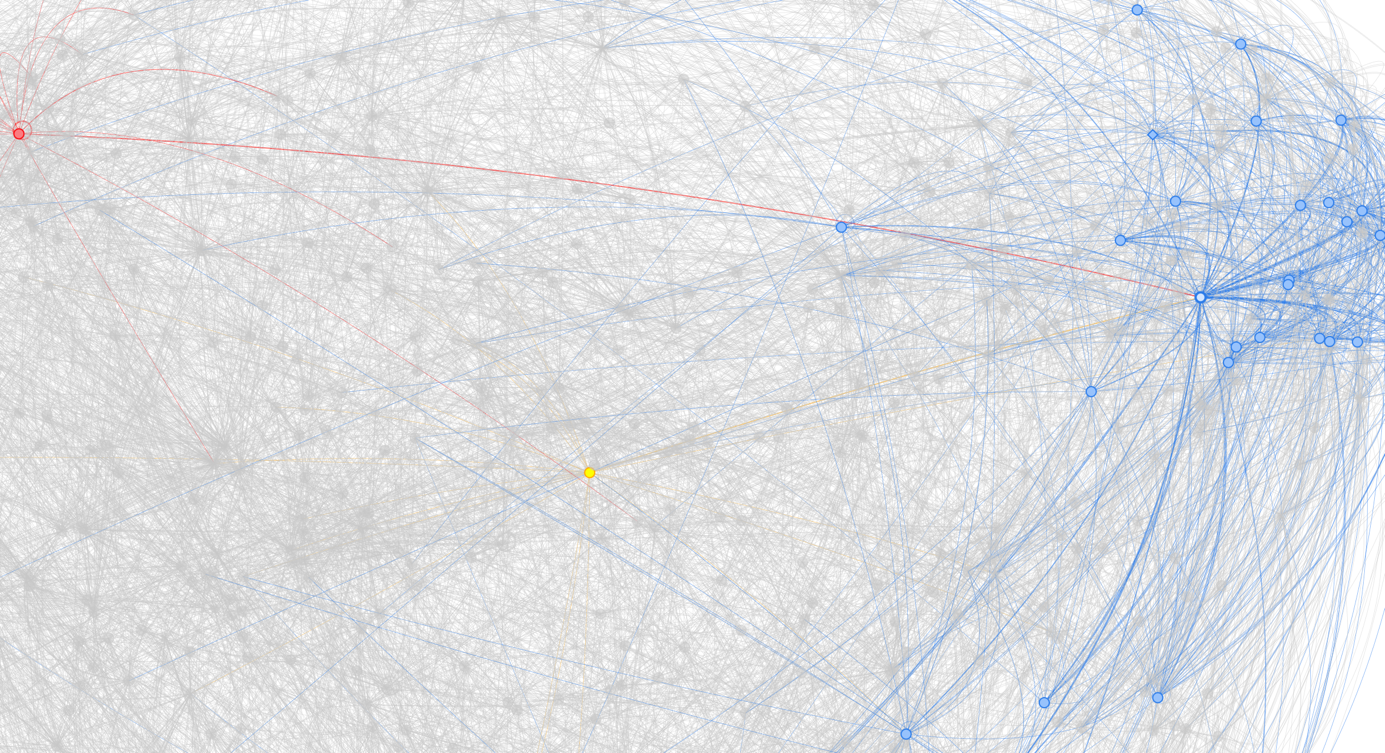
\includegraphics[width=\textwidth]{figures/media/image33.png}
  \caption{\label{fig:pds-vernetzung}Vernetzung des FE \cluster{02\_Pds} (rechts) im Gesamt-Frame.}
\end{figure}
\newpage
Als Partei am linksäußeren Rand, die zudem als bedeutungsähnlich zur NPD im vorangehenden Zeitraum identifiziert wurde (siehe Tabelle 3 im Anhang), soll das FE \cluster{02\_Pds} als Teil eines Linksextremismus-Frames in den Blick genommen werden. Wie in \figref{fig:pds-vernetzung} ersichtlich, ist das FE fast ausschließlich im thematischen Bereich der Innenpolitik vernetzt, wobei insbesondere die Anbindung an die FE \cluster{02\_Npd} und \cluster{02\_Autonomen{\breakbar}Antifa{\breakbar}Rechtsextremisten (politischer Extremismus)} ein Framing als extremistische Partei andeuten. Das FE \cluster{02\_Norden{\breakbar}Süden{\breakbar}Osten} aus der Community ‚Krieg \& Islamismus` (links in der Abbildung) verweist außerdem auf den regional begrenzten Erfolg der Partei. Auch das angebundene FE \cluster{02\_Zusammenarbeit{\breakbar}Kooperation} aus dem Bereich ‚Staat, FdGO \& Gesellschaft` (in der Mitte der Abbildung) zeigt eine besondere Rolle der PDS im Parteienspektrum an, da in Frage steht, inwiefern eine Zusammenarbeit in einer Koalition, wie sie in Berlin auf Landesebene seit 2001 besteht, gerechtfertigt ist (siehe Belege K05--K07 in \tabref{tab:K05-K07}).

\begin{table}
\caption{Konkordanzen zur Kollokation der Cluster \cluster{02\_Pds} und \cluster{02\_Zusammenarbeit{\breakbar}Kooperation}.}
\label{tab:K05-K07}
K05 spiegel\_461705
\begin{tabularx}{\textwidth}{QQQ}
\toprule
und Csu-chef\_Stoiber lehnten eine große\_Koalition nach der Wahl am lt100 September ab Schröder schloss eine & {[}\cluster{02\_Zusammenarbeit{\breakbar}Kooperation}: \textbf{Zusammenarbeit}{]}\newline
\textbf{mit der}\newline
{[}\cluster{02\_Pds}: \textbf{Pds}{]} & aus in dem Fernsehduell flammte der Streit über die Finanzierung des Wiederaufbaus nach der Flut \\
\bottomrule
\end{tabularx}
\bigskip \newline
K06 spiegel\_723618
\begin{tabularx}{\textwidth}{QQQ}
\toprule
alleinige\_Schuld an dem Wahldebakel in die Schuhe Matschie habe mit seiner sehr rigiden Ablehnung einer & {[}\cluster{02\_Zusammenarbeit{\breakbar}Kooperation}: \textbf{Zusammenarbeit}{]}\newline
\textbf{mit der}\newline
{[}\cluster{02\_Pds}: \textbf{Pds}{]} & die Wähler geradezu\_ermuntert den Linkssozialisten ihre Stimme zu geben sagte Dewes die Pds kam am\_Sonntag \\
\bottomrule
\end{tabularx}
\bigskip \newline
K07 taz\_795267
\begin{tabularx}{\textwidth}{QQQ}
\toprule
Liste aufstellen um bei dem Zugriffsverfahren auch Chancen zu haben eine andere Möglichkeit wäre die & {[}\cluster{02\_Zusammenarbeit{\breakbar}Kooperation}: \textbf{Kooperation}{]}\newline
\textbf{zwischen Fdp Bürgerbündnis und}\newline
{[}\cluster{02\_Pds}: \textbf{Pds}{]} & nur mit den Rechtsaußen will keiner die werden sich wohl wieder damit revanchieren dass sie \\
\bottomrule
\end{tabularx}
\end{table}

Das FE \cluster{02\_Autonomen{\breakbar}Antifa{\breakbar}Rechtsextremisten (Politischer Extremismus)} letztlich kondensiert als einziges FE neben den besprochenen Parteien den zeitgenössischen politischen Extremismus. Während dieser im Vorjahr noch in mehreren Clustern repräsentiert war und dabei ein von gewaltvollen Straftaten geprägtes Framing aufwies, sind in diesem Zeitraum der politische Bereich mit Bezügen zu Parteien (\cluster{02\_Parteien}, \cluster{02\_Pds}, \cluster{02\_Npd}), Gesetzen (\cluster{02\_Agenda\_2010{\breakbar}Reformen{\breakbar}Hartz\_Iv}) und Gewerkschaften (\cluster{02\_verdi{\breakbar}Dienstleistungsgewerkschaft\_Verdi{\breakbar}Gewerkschaft\_Verdi}) sowie zu Demonstrationen prägend. Dies geht auch auf die breite Semantik des Clusters, das mit 147 Wörtern sehr groß ist, zurück und etwa auch die \emph{Montagsdemonstrationen} gegen die Agenda 2010 umfasst, zurück. Ein extremistisches Framing manifestiert sich in den attributiven FE wie \cluster{02\_Intoleranz{\breakbar}Hetze{\breakbar}Rassismus} und \cluster{02\_Antisemitismus}, während Gewalt nur noch einen deutlich geringeren Teil des Frames ausmacht und sich etwa in den FE \cluster{02\_Randalierer{\breakbar}Wasserwerfer{\breakbar}Maschinenpistolen} und \cluster{02\_Razzien{\breakbar}Festnahmen{\breakbar}Verhaftungen} zeigt.

\subsubsection{Islamismus}\label{islamismus-1}

Für den Bereich des Islamismus liegt mit den datengeleitet identifizierten Clustern bereits eine Fülle an relevanten FE vor, die nur schlaglichtartig und in grundlegenden Tendenzen analysiert werden können.

Als Kernbestandteile des Frames werden die folgenden Cluster aufgefasst und an dieser Stelle bereits in Teil-Frames gegliedert: Einen Teil-Frame zum Nahostkonflikt bilden die FE \cluster{02\_Tulkarm{\breakbar}Tulkarem{\breakbar}jüdische\_Siedler (Nahostkonflikt)}, \cluster{02\_Hebron{\breakbar}Nablus{\breakbar}Rafah (Orte im Nahostkonflikt)}, \cluster{02\_Gaza{\breakbar}Ramallah{\breakbar}Tel\_Aviv (Orte im Nahostkonflikt \& israelische Armee)}, \cluster{02\_Gaza-streifen{\breakbar}Westjordanland{\breakbar}Gazastreifen (Orte im Nahostkonflikt)}, \cluster{02\_Israelis{\breakbar}Palästinenser{\breakbar}Palästinensern}, \cluster{02\_israelischen{\breakbar}israelische{\breakbar}palästinensische}, \cluster{02\_Palästinenserpräsident\_Jassir\_Arafat{\breakbar}Jassir\_Arafat{\breakbar}Abbas (Nahostkonflikt)}. Ein weiterer wesentlicher Teil des Islamismus-Frames umfasst FE, die mit den Anschlägen des 11. Septembers assoziiert sind. Hier finden sich die islamistische Gruppierungen Al-Qaida, die die Anschläge verübte sowie der Diktator Saddam Hussein, dem durch die USA Verbindungen zu Al-Qaida vorgeworfen wurde und dessen Sturz durch die USA im Rahmen des Irakkrieges forciert wurde: \cluster{02\_Al\_Qaida{\breakbar}al-Qaida{\breakbar}Extremisten (islamistische Akteure)}, \cluster{02\_Qaida{\breakbar}Terrorgruppe{\breakbar}Terrororganisation (terroristische Gruppen und Anschläge)}, \cluster{02\_Taliban-Kämpfer{\breakbar}Al-Qaida-Kämpfer{\breakbar}Afghanen (Akteure Islamismus)}, \cluster{02\_Saddam\_Hussein{\breakbar}Saddam}, \cluster{02\_Saddam\_Husseins{\breakbar}Saddams{\breakbar}Hussein}.

Der Nahostkonflikt wird insgesamt ähnlich geframet wie im vorigen Zeitraum. Es finden sich im Bereich ‚Krieg \& Islamismus` zahlreiche FE, die auf gewaltvolles kriegerisches Handeln sowie das Begehen von Anschlägen hindeuten. Die Communities ‚Innenpolitik` und ‚Außenpolitik` verdeutlichen dabei insbesondere diplomatische Bemühungen und die Community ‚Staat, FdGO \& Gesellschaft` darüber hinaus den durch Religion und terroristisches handeln geprägten Charakter des Konfliktes (\cluster{02\_Terrormis{\breakbar}Terror}, \cluster{02\_Juden}, \cluster{02\_Antismeitismus}, \cluster{02\_christliche{\breakbar}islamische{\breakbar}muslimische}, \cluster{02\_Moslems{\breakbar}Christen{\breakbar}Muslime}).

Am übrigen Teil des Islamismus-Frames, der das verstehensrelevante Wissen um den Irakkrieg und die Anschläge vom 11. September 2001 beinhaltet, sind insbesondere die Netzwerk-Cluster ‚Krieg \& Islamismus` sowie ‚Straftaten \& Juristisches` beteiligt. In ersterem tragen zum Islamismus-Framing FE, die den Irak bzw. das Regime Saddam Husseins als Ort bzw. Akteur des Krieges benennen, bei (u.\,a. \cluster{02\_Irak}, \cluster{02\_irakischen{\breakbar}irakische}, \cluster{02\_Saddam\_Husseins{\breakbar}Saddams{\breakbar}Hussein}, \cluster{02\_Regime}); zum anderen auch die durch die US-Regierung angeführte Begründung der Vermutung von Massenvernichtungswaffen (\cluster{02\_Massenvernichtungswaffen}, \cluster{02\_chemischen{\breakbar}chemische{\breakbar}Chemiewaffen (Chemiewaffen \& Atombombe)} und Kriegshandlungen (u.\,a. \cluster{02\_Anschläge{\breakbar}Attentate{\breakbar}Terroranschläge}, \cluster{02\_Attentäter{\breakbar}Selbstmordattentäter}, \cluster{02\_Angriffe}). Im thematischen Teil-Frame ‚Straftaten \& Juristisches` finden sich darüber hinaus FE um das US-Gefangenenlager Guantánamo (\cluster{02\_Guantánamo{\breakbar}Guantanamo{\breakbar}Guantanamo\_Bay}, \cluster{02\_Gefangenen}) sowie solche, die für Kriegskontexte typische epistemische Unsicherheiten zum Ausdruck bringen (\cluster{02\_Verdacht}, \cluster{02\_vorgeworfen}, \cluster{02\_Anzeichen\_dafür{\breakbar}Hinweise\_darauf{\breakbar}Befürchtung}, \cluster{02\_Anschuldigungen{\breakbar}Drohungen{\breakbar}Behauptungen}, \cluster{02\_Hinweise}). Im thematischen Feld der ‚Außenpolitik` treten insbesondere die westlichen Kriegsakteure (u.\,a. \cluster{02\_Bush{\breakbar}Blair}, \cluster{02\_Us-regierung}) hervor, aber auch Schlagwörter wie das der von Bush geprägten ‚Achse des Bösen` (\cluster{02\_Bösen{\breakbar}Achse}). Im Bereich ‚Innenpolitik` sind hingegen nur einzelne FE wie \cluster{02\_Erklärung}, \cluster{02\_Frage\_ob}, \cluster{02\_unterstützen{\breakbar}unterstützt} sowie \cluster{02\_Gruppe}, \cluster{02\_Mitgliedern} angebunden. Dies verdeutlicht, dass in einem solchen Konflikt immer wieder Fragen nach Legitimität sowie der Zugehörigkeit zu Allianzen bzw. einzelnen beteiligten Gruppen gestellt werden.

\subsubsection{Fazit}\label{fazit-1}

Insgesamt ist zum Extremismus-Frame des Zeitraumes 2002--2004 eine deutliche Verlagerung der im Diskurs evozierten Wissensbestände auf den Bereich des Islamismus festzustellen. Nach den Anschlägen vom 11. September 2001 und mit dem beginnenden Irakkrieg wird diese Extremismusform zum zentralen Gegenstand der Berichterstattung, was sich in einer Vielzahl an Clustern, die als Teil dieses Frames gelesen werden können, niederschlägt, während der politische Extremismus im wesentlichen als historisches Phänomen und in einer Erinnerungsperspektive an die Zeit des Nationalsozialismus Bestandteil des Frames ist. Hier finden sich nur einzelne FE, die zeitgenössische extremismusbezogene Entwicklungen abbilden, etwa zu den Parteien NPD und PDS sowie einem semantisch vagen Wort-Cluster \cluster{02\_Autonomen{\breakbar}Antifa{\breakbar}Rechtsextremisten}, das neben Gruppen des politischen Extremismus u.\,a. auch die Montagsdemonstrationen umfasst. In der Möllemann-Affäre spielt auch der Vorwurf des Antisemitismus als einem wesentlichen Kennzeichen des Rechtsextremismus eine Rolle. Mit dieser Entwicklung einher geht das weitestgehende Verschwinden der Assoziation mit gewalttätigen Straftaten, die im vorigen Zeitraum noch deutlich ausgeprägt war. Ein Vergleich der Parteien NPD und PDS zeigt außerdem, dass die NPD durch die diversen FE mit Bezug zum Verbotsverfahren deutlich als rechtsextreme zu bekämpfende Bedrohung geframet wird, während die PDS in weiten Teilen als gewöhnliche, im politischen Tagesgeschäft agierende Partei konstruiert wird. Bei ihr deutet lediglich die Diskussion der Legitimität einer Zusammenarbeit sowie die Frame-Relationen zum politischen Extremismus (\cluster{02\_Autonomen{\breakbar}Antifa{\breakbar}Rechtsextremisten}) und der NPD an, dass ihr nicht der Status einer Mittepartei zugemessen wird.

\subsection{Der Zeitraum 2005--2007}\label{der-zeitraum-2005-2007}

\subsubsection{\texorpdfstring{\emph{Corpus-driven} Voranalyse: Thematisch gruppierte Auswahl semantisch äquivalenter Cluster im Vergleich zu den Kern-FE des vorigen Zeitraums}{Corpus-driven Voranalyse: Thematisch gruppierte Auswahl semantisch äquivalenter Cluster im Vergleich zu den Kern-FE des vorigen Zeitraums}}\label{corpus-driven-voranalyse-thematisch-gruppierte-auswahl-semantisch-aequivalenter-cluster-im-vergleich-zu-den-kern-fe-des-vorigen-zeitraums-1}

Bevor einzelne Extremismusvarianten-Frames für diesen Zeitraum erstellt werden, wurden erneut die im Vektorraum nächsten Cluster zu den betrachteten Clustern des vorigen Zeitraumes ermittelt. Tabelle 4 im Anhang zeigt die Ergebnisse der Analyse und \tabref{tab:2005} ordnet die identifizierten Cluster einzelnen Extremismusvarianten-Frames zu.

\begin{table}[h]
\small
\caption{Thematisch gruppierte Auswahl semantisch äquivalenter Cluster des Zeitraums 2005--2007.}
\label{tab:2005}
 \begin{tabularx}{\textwidth}{>{\hsize=0.5\hsize}X >{\hsize=0.5\hsize}X >{\hsize=2.0\hsize}X}
  \lsptoprule
  Extremismus-Variante & Bezug & Frame-Elemente \\
  \midrule
  \multirow{2}{=}{Rechts\-ex\-tre\-mis\-mus} 
  & historisch & \cluster{Nationalsozialismus{\breakbar}Ns-zeit{\breakbar}Holocaust, Nazis{\breakbar}Hitler, 1945{\breakbar}Zweiten\_Weltkrieg{\breakbar}Kriegsende} \\
  & zeit\-ge\-nössisch & \cluster{Rechtsextremen{\breakbar}Rechtsextremisten{\breakbar}Neonazis} \\
  \midrule
  \multirow{2}{=}{Links\-ex\-tre\-mis\-mus} 
  & zeit\-ge\-nössisch & \cluster{Pds{\breakbar}Linkspartei{\breakbar}WASG, Heiligendamm{\breakbar}G-8-Gipfel} \\
  & historisch & \cluster{Raf} \\
  \midrule
  \multirow{2}{=}{Politischer Extremismus} 
  & historisch & \cluster{Kommunismus{\breakbar}Sowjetunion{\breakbar}Weimarer\_Republik, KZs{\breakbar}Konzentrationslager{\breakbar}Deportationen, Ss{\breakbar}Gestapo{\breakbar}Wehrmacht} \\
  & zeit\-ge\-nössisch & \cluster{Wahlalternative{\breakbar}LinksparteiPDS{\breakbar}Wahlalternative\_Arbeit, Gegendemonstranten{\breakbar}Antifas{\breakbar}Kundgebungen} \\
  \midrule
  {Islamismus} & Nahost\-konflikt & \cluster{Hisbollah-miliz{\breakbar}Luftangriffe{\breakbar}israelische\_Armee, Mahmud\_Abbas{\breakbar}Palästinenserpräsident\_Abbas, Gazastreifen{\breakbar}Gaza-streifen{\breakbar}Westjordanland, Palästinenserpräsident\_Mahmud\_Abbas{\breakbar}Ramallah, Beirut{\breakbar}Gaza{\breakbar}Tel\_Aviv, Olmert{\breakbar}Abbas{\breakbar}Scharon, Hamas{\breakbar}Hisbollah{\breakbar}Fatah, Palästinenser{\breakbar}Israelis} \\
  & Irakkrieg & \cluster{Qaida{\breakbar}Todesschwadronen{\breakbar}Terrorgruppen, Saddam\_Hussein{\breakbar}Saddam} \\
  \midrule
  varianten\-über\-greifend & allgemein & \cluster{rechtsextremen{\breakbar}rechtsextremistischen{\breakbar}rechtsextreme, Intoleranz{\breakbar}Antisemitismus{\breakbar}Hetze} \\
  \lspbottomrule
 \end{tabularx}
\end{table}

\subsubsection{\texorpdfstring{\emph{Corpus-driven} Voranalyse: Cluster mit hoher Cosinus-Distanz im Vergleich zum vorigen Zeitraum}{Corpus-driven Voranalyse: Cluster mit hoher Cosinus-Distanz im Vergleich zum vorigen Zeitraum}}\label{corpus-driven-voranalyse-cluster-mit-hoher-cosinus-distanz-im-vergleich-zum-vorigen-zeitraum-1}


\begin{table}[t]\small
  \caption{Cluster mit hoher Cosinus-Distanz im Vergleich zum vorigen Zeitraum.}
  \label{tab:cluster-high-cosine-distance-2005}
  \begin{tabularx}{\textwidth}{X r}
    \lsptoprule
    Cluster & Cos.-Dist. \\
    \midrule
    \cluster{Heiligendamm{\breakbar}G-8-Gipfel} & 0.46 \\
    \cluster{Karikaturen{\breakbar}Mohammed-Karikaturen} & 0.42 \\
    \cluster{Bundespolizei} & 0.39 \\
    \cluster{Schily{\breakbar}Schäuble{\breakbar}Steinmeier} & 0.28 \\
    \cluster{Großen\_Koalition{\breakbar}großen\_Koalition} & 0.25 \\
    \cluster{Pds{\breakbar}Linkspartei{\breakbar}WASG} & 0.25 \\
    \cluster{Nicolas\_Sarkozy{\breakbar}de\_Villepin{\breakbar}Jacques\_Chirac} & 0.24 \\
    \cluster{Seehofer{\breakbar}Huber{\breakbar}Oettinger} & 0.23 \\
    \cluster{Libanon} & 0.22 \\
    \cluster{Hamas{\breakbar}Hisbollah{\breakbar}Fatah} & 0.22 \\
    \cluster{Berlusconi{\breakbar}Prodi} & 0.22 \\
    \cluster{Saddam\_Hussein{\breakbar}Saddam} & 0.2 \\
    \cluster{Schmiergeldzahlungen{\breakbar}schwarze\_Kassen{\breakbar}Schmiergelder} & 0.2 \\
    \cluster{Leyen{\breakbar}Leyen\_Cdu} & 0.2 \\
    \cluster{Angela\_Merkel{\breakbar}Merkel{\breakbar}Kanzlerin} & 0.2 \\
    \cluster{Olmert{\breakbar}Abbas{\breakbar}Scharon} & 0.19 \\
    \cluster{mutmaßliche\_Täter{\breakbar}Uwe\_K{\breakbar}Mario\_M} & 0.19 \\
    \cluster{OEF{\breakbar}Isaf{\breakbar}Operation\_Enduring\_Freedom} & 0.19 \\
    \cluster{Bundespräsident\_Horst\_Köhler{\breakbar}Bundespräsident\_Köhler{\breakbar}Horst\_Köhler} & 0.19 \\
    \cluster{Dick\_Cheney{\breakbar}Mccain{\breakbar}Hillary\_Clinton} & 0.18 \\
    \lspbottomrule
  \end{tabularx}
\end{table}

Die in \tabref{tab:cluster-high-cosine-distance-2005} enthaltenen Cluster weisen die größte Distanz im Vektorraum im Vergleich zum Vorjahr auf. Es kristallisieren sich in diesen Resultaten die folgenden Themen heraus, die für den Extremismusdiskurs von Bedeutung sind: Der G8-Gipfel in Heiligendamm 2007, anlässlich dessen es Proteste linker Gruppen gab (\cluster{05\_Heiligendamm{\breakbar}G-8-Gipfel}), die Mohammed-Karikaturen aus dem September 2005 (\cluster{05\_Karikaturen{\breakbar}Mohammed-Karikaturen}), die Fusion von WASG und PDS zur Linkspartei (\cluster{05\_Pds{\breakbar}Linkspartei{\breakbar}WASG}) sowie der 2006 beginnende Libanon-Krieg (\cluster{05\_Libanon}, \cluster{05\_Hamas{\breakbar}Hisbollah{\breakbar}Fatah}).

\subsubsection{Rechts- und Linksextremismus}\label{rechts--und-linksextremismus-2}

Es treten in diesem Zeitraum zwei FE zu Tage, die sich keinen einzelnen Extremismusformen zuschreiben lassen, sondern sich auf alle Formen gleichermaßen beziehen. Dies ist zum einen das FE \cluster{05\_Intoleranz{\breakbar}Antisemitismus{\breakbar}Hetze}, das Charakteristika von Extremismus -- einige darunter mit besonderem Bezug zum Rechtsextremismus -- wie \emph{Antisemitismus}, \emph{Rassismus} und \emph{Intoleranz} sowie unterschiedliche Begriffe des Wortfeldes ‚Ausgrenzung` enthält (u.\,a. \emph{Diskriminierung}, \emph{Vorurteile}, \emph{Zensur}). Es weist vor allem Verbindungen zum Bereich ‚Staat, FdGO \& Gesellschaft` auf (\cluster{05\_Kampf\_gegen}, \cluster{05\_Schwule{\breakbar}Lesben{\breakbar}Schwulen}, \cluster{05\_Islam{\breakbar}Religion}, \cluster{05\_Kopftuch}), wobei auch Terrorismus und Gewalt (\cluster{05\_Terror{\breakbar}Terrorismus{\breakbar}Gewalt}) sowie rechtsextreme Akteure (\cluster{05\_Nazis{\breakbar}Hitler}, \cluster{05\_Rechtsextremen{\breakbar}Rechtsextremisten{\breakbar}Neonazis}) Bezugspunkte darstellen und die Aufnahme in den Extremismus-Frame rechtfertigen.

Das zweite Cluster \cluster{05\_rechtsextremen{\breakbar}rechtsextremistischen{\breakbar}rechtsextreme} ist in seiner Semantik vergleichsweise vage und umfasst sowohl Attribute (etwa \emph{rechtesextremen}, \emph{islamistische}), Akteure (\emph{Freien\_Kameradschaften}, \emph{Skinheads}, \emph{V-leute}) als auch Praktiken (\emph{Überfälle}, \emph{verüben}). Ganz im Gegensatz zum zuvor betrachteten FE weist es kaum Verbindungen im Bereich ‚Staat, FdGO \& Gesellschaft` auf, sondern knüpft insbesondere an die Themen ‚Krieg \& Islamismus` (u.\,a. \cluster{05\_Bombenanschlag{\breakbar}Selbstmordanschlag{\breakbar}Überfall}, \cluster{05\_Angriffe{\breakbar}Attacken{\breakbar}Angriffe}), ‚Straftaten \& Juristisches` (u.\,a. \cluster{05\_Gewalttaten{\breakbar}Straftaten{\breakbar}Morde}, \cluster{05\_Tat}, \cluster{05\_Bundeskriminalamt{\breakbar}Bka{\breakbar}Verfassungsschutz}) sowie ‚Demonstrationen \& politischer Extremismus` (\cluster{05\_Demonstrationen{\breakbar}Proteste{\breakbar}Protesten}, \cluster{05\_Verbot}) an.

Eine Reihe von Clustern bezieht sich etwas spezifischer auf den Bereich des politischen Extremismus. Dies sind in einer historischen Perspektive die FE \cluster{05\_Kommunismus{\breakbar}Sowjetunion{\breakbar}Weimarer\_Republik (Totalitarismus, 68er, Weimarer Republik)}, \cluster{05\_KZs{\breakbar}Konzentrationslager{\breakbar}Deportationen (NS- und DDR-Zeit)} und \cluster{05\_Ss{\breakbar}Gestapo{\breakbar}Wehrmacht (staatliche Akteure NS- \& DDR-Zeit)}. Diese FE zeigen durch die Bündelung von staatlichen Akteuren wie \emph{Ss}, \emph{Gestapo} und \emph{Staatssicherheit} im Cluster \cluster{05\_Ss{\breakbar}Gestapo{\breakbar}Wehrmacht} oder (Resultaten) totalitärer Praktiken wie \emph{KZs}, \emph{Gulag}, \emph{Machtergreifung} und \emph{Berliner\_Mauer} im Cluster \cluster{05\_KZs{\breakbar}Konzentrationslager{\breakbar}Deportationen} jeweils eine im Diskurs konstituierte (paradigmatische) Ähnlichkeit der Regime zueinander auf, die in der Politikwissenschaft als Totalitarismustheorie verhandelt wird.

Der Rechtsextremismus-Frame dieses Zeitraumes umfasst erneut einige FE, die einen Teil-Frame zur NS-Zeit bilden: \cluster{05\_Nationalsozialismus{\breakbar}Ns-zeit{\breakbar}Holocaust}, \cluster{05\_Nazis{\breakbar}Hitler}, \cluster{05\_1945{\breakbar}Zweiten\_Weltkrieg{\breakbar}Kriegsende (Kriegsende Zweiter Weltkrieg)}. Auch die unter dem Frame zum politischen Extremismus subsummierten FE sind durch ihre Relation zu den Kern-Clustern Teil des Frames zur NS-Zeit. Insgesamt ist dieser Teil des Rechtsextremismus-Frames in diesem Zeitraum stärker im Cluster ‚Staat, FdGO \& Gesellschaft` verankert, was eine stärkere Fokussierung der Berichterstattung auf die historisch-gesellschaftliche Dimension denn auf die kriegerischen Handlungen andeutet.

Als weiteres zentrales FE des Rechtsextremismus-Frames ist \cluster{05\_Rechtsextremen{\breakbar}Rechtsextremisten{\breakbar}Neonazis (Akteure des Rechtsextremismus)} zu nennen. Es prägt einen Großteil seiner Verbindungen in das Cluster ‚Innenpolitik` aus, was darauf zurückgeht, dass es den frequenten Ausdruck \emph{Npd} beinhaltet. Neben den FE, die es als politische Partei ausweisen (u.\,a. \cluster{05\_Bundestagswahl{\breakbar}Landtagswahl}, \cluster{05\_Landtagswahlen}, \cluster{05\_Stimme}) finden sich hier auch FE wie \cluster{05\_Sachsen-anhalt{\breakbar}Mecklenburg-vorpommern{\breakbar}Sachsen (ostdeutsche Bundesländer)}, die auf den regional begrenzten Erfolg der Partei verweisen sowie \cluster{05\_Demokraten{\breakbar}Republikaner} und \cluster{05\_Pds{\breakbar}Linkspartei{\breakbar}WASG}, die -- als einzige angeschlossene Parteien und wie bereits im vergangenen Zeitraum -- eine Stellung der Partei abseits der Mitte verdeutlichen. Die starke Verhaftung im Bereich des ‚Juristischen` ist nun, nach Abschluss des ersten NPD-Verbotverfahrens, verschwunden. Stattdessen zeigt sich eine Verschiebung in den Bereich der ‚Demonstrationen \& des politischen Extremismus`, die vor allem die Beteiligung an Demonstrationen durch rechtsextreme Akteure hervorhebt. Das Framing als gewalttätige Form des Extremismus zeigt sich auch in diesem Zeitraum kaum. Lediglich das angebundene FE \cluster{05\_rechtsextremen{\breakbar}rechtsextremistischen{\breakbar}rechtsextreme (Extremismus)} enthält einige Begriffe, die auf gewaltvolles Handeln hindeuten, wie z.\,B. \emph{gewalttätigen} oder \emph{Brandanschläge}. Wie auch in den Vorjahren sind die Bekämpfung von Rechtsextremismus (u.\,a. \cluster{05\_Kampf\_gegen}, \cluster{05\_Bekämpfung{\breakbar}zur\_Bekämpfung{\breakbar}bekämpfen}, \cluster{05\_Umgang}, \cluster{05\_Strategie}) sowie Kennzeichen von Extremismusformen und Unterdrückung (\cluster{05\_Intoleranz{\breakbar}Antisemitismus{\breakbar}Hetze}) Teil des Framings.

Zur Modellierung des Linksextremismus-Frames sind die Cluster \cluster{05\_Raf}, \cluster{05\_Pds{\breakbar}Linkspartei{\breakbar}WASG} und \cluster{05\_Heiligendamm{\breakbar}G-8-Gipfel} einschlägig. Der G8-Gipfel weist dabei eine Vielzahl an Frame-Relationen in die Bereiche ‚Innen- und Außenpolitik` auf (u.\,a. \cluster{05\_Treffen}, \cluster{05\_Blair{\breakbar}Tony\_Blair{\breakbar}Chirac}, \cluster{05\_Außenminister{\breakbar}Regierungschefs{\breakbar}Botschafter}). Er wird jedoch gleichermaßen durch FE des thematischen Teil-Frames ‚Demonstrationen \& politischer Extremismus` als Ereignis geframet, das von starkem Protest begleitet wurde (u.\,a. \cluster{05\_Protest{\breakbar}Widerstand{\breakbar}Protest\_gegen}, \cluster{05\_Demonstranten}) und auch durch politisch-extremistische Elemente geprägt war (\cluster{05\_Gegendemonstranten{\breakbar}Antifas{\breakbar}Kundgebungen}), wie die Belegstellen zur Kollokation der beiden Cluster verdeutlichen (siehe \tabref{tab:K08-K10}).

\begin{table}[h]\small
  \caption{Konkordanzen zur Kollokation der Cluster \cluster{05\_Heiligendamm{\breakbar}G-8-Gipfel} und \cluster{05\_Gegendemonstranten{\breakbar}Antifas{\breakbar}Kundgebungen}.}
  \label{tab:K08-K10}
  K08 welt\_1203355
\begin{tabularx}{\textwidth}{QQQ}
\toprule
in Hamburg muss auch dem neutralen\_Beobachter klar sein dass sich der Protest\_gegen das Treffen von & {[}\cluster{05\_Heiligendamm{\breakbar}G-8-Gipfel:} \textbf{Heiligendamm}{]}\newline
\textbf{verselbstständigt hat einem Teil der}\newline
{[}\cluster{05\_Gegendemonstranten{\breakbar}Antifas{\breakbar}Kundgebungen}: \textbf{G-8-Gegner}{]} & geht es ganz grundsätzlich um die Machtfrage um ein archaisches Fanal des Widerstands schlechthin deshalb \\
\bottomrule
\end{tabularx}
\bigskip \newline
K09 spiegel\_1189419
\begin{tabularx}{\textwidth}{QQQ}
\toprule
Demonstrationen angesagt am Myfest in Kreuzberg und im Berliner Mauerpark vor\_allem der baldige G8-Gipfel in & {[}\cluster{05\_Heiligendamm{\breakbar}G-8-Gipfel:} \textbf{Heiligendamm}{]}\newline
\textbf{lässt es unsicher erscheinen ob}\newline
{[}\cluster{05\_Gegendemonstranten{\breakbar}Antifas{\breakbar}Kundgebungen}: \textbf{Autonome}{]} & nicht dann die Gelegenheit zu heftigeren Krawallen nutzen wollen bemerkenswert ist in jedem\_Fall wie ruhig \\
\bottomrule
\end{tabularx}
\bigskip \newline
K10 spiegel\_1211355
\begin{tabularx}{\textwidth}{QQQ}
\toprule
Zeltlager\_errichtet mal gegen mal für eine Weltregierung demonstriert und mal am Zaun rüttelt eine politische & {[}\cluster{05\_Gegendemonstranten{\breakbar}Antifas{\breakbar}Kundgebungen}: \emph{\textbf{Protestbewegung}}{]}\newline
\textbf{die an den}\newline
{[}\cluster{05\_Heiligendamm{\breakbar}G-8-Gipfel:} \emph{\textbf{G-8-Gipfel}}{]} & einerseits radikale Forderungen richtet und ihn andererseits verhindern will - eine Bewegung also die nicht \\
\bottomrule
\end{tabularx}
\end{table}

Anders als später beim Hamburger G-20-Gipfel im Zeitraum 2017--2019 ist Gewalt jedoch kein wesentlicher Bestandteil des Framings. Des Weiteren ist der Zusammenschluss der beiden linken Partei PDS und WASG im Jahr 2007 durch das FE \cluster{05\_Pds{\breakbar}Linkspartei{\breakbar}WASG} im Frame abgebildet. Erneut ist -- zugunsten einer klaren Verankerung im Bereich der Innenpolitik -- die Assoziation mit dem Thema ‚Extremismus` nur punktuell sichtbar; etwa in den FE \cluster{05\_rechtsextremen{\breakbar}Rechtsextremisten{\breakbar}Neonazis} sowie \cluster{05\_Zusammenarbeit{\breakbar}Kooperation}. Auch die Bezüge in das thematische Feld ‚Demonstrationen \& politischer Extremismus` beschränken sich auf die FE \cluster{05\_Hartz\_Iv}, \cluster{05\_ausgesprochen{\breakbar}gestimmt} sowie \cluster{05\_Bürgerbegehren{\breakbar}Volksbegehren{\breakbar}Bürgerentscheid (Volksentscheide \& Umbenennung)}, wobei der größte Teil der Kookkurrenzen mit letzterem Cluster durch das in diesem enthaltene Wort \emph{Umbenennung} erklärbar ist.

Anlässe für die in diesem Zeitraum verstärkte Thematisierung der RAF (das Cluster weist eine sehr hohe Keyness von 884,5 \emph{Log-Likelihood} auf) ist die Eröffnung einer kontroversen Ausstellung RAF-Ausstellung in Berlin, das Erscheinen mehrerer Bücher und Filme zum Thema sowie der 30. Jahrestag der Entführung von Hanns Martin Schleyer. Die RAF weist, im Gegensatz zu den anderen FE des politischen Extremismus, ein Framing auf, das stark durch die Bereiche ‚Straftaten \& Juristisches` sowie ‚Krieg \& Islamismus` geprägt ist und einerseits durch gewaltvolles Handeln (\cluster{05\_Gewalttaten{\breakbar}Straftaten{\breakbar}Morde}, \cluster{05\_Entführung{\breakbar}Ermordung}, \cluster{05\_Terror{\breakbar}Terrorismus{\breakbar}Gewalt}), andererseits durch Gefängnisstrafen (\cluster{05\_Häftlinge{\breakbar}Gefangene{\breakbar}Gefangenen}) sowie Straftäter*innen, Opfer und Ermittlungen (\cluster{05\_mutmaßliche\_Täter{\breakbar}Uwe\_K{\breakbar}Mario\_M}) geprägt ist. Die Gruppe wird dabei explizit als terroristisch beschrieben oder mit terroristischen Gruppierungen verglichen, was sich in der Relation zu den FE \cluster{05\_Extremisten{\breakbar}Islamisten{\breakbar}Aufständischen (extremistische Akteure)}, \cluster{05\_Qaida{\breakbar}Todesschwadronen{\breakbar}Terrorgruppen (Islamismus{\slash}Terrorismus)} und \cluster{05\_Terror{\breakbar}Terrorismus{\breakbar}Gewalt} zeigt. Die in \tabref{tab:K11-K14} dargestellten Instanzen der Kollokation mit dem Cluster \cluster{05\_Extremisten{\breakbar}Islamisten{\breakbar}Aufständischen} illustrieren dies näher: Während die RAF in den Belegen K11 und K14 eindeutig als terroristische Gruppe beschrieben wird, wird sie in Beleg K12 punktuell mit Al-Qaida gleichgesetzt. In Beleg K13 wiederum wird durch die Interviewerin gefragt, ob „al-Qiada nicht\_ungleich gefährlicher als es die Raf war`` sei, was durch den interviewten Politikwissenschaftler bejaht wird. Hier finden sich also metadiskursive Spuren für die den sozialwissenschaftlichen Extremismusdikurs prägenden Debatte um die im Extremismuskonzept angelegte Gleichsetzung verschiedener Extremismusformen bzw. extremistischer Gruppen.
\largerpage

\begin{table}\small
  \caption{Konkordanzen zur Kollokation der Cluster \cluster{05\_Raf} und \cluster{05\_Extremisten{\breakbar}Islamisten{\breakbar}Aufständischen}.}
  \label{tab:K11-K14}
K11 welt\_1237479
\begin{tabularx}{\textwidth}{QQQ}
\toprule
Ermittler gegen Mitglieder der Militanten\_Gruppe sollte nicht kleingeredet werden zwar wurden nicht Terroristen der Kategorie & {[}\cluster{05\_Raf}: \textbf{Raf}{]}\newline
\textbf{oder}\newline
{[}\cluster{05\_Extremisten{\breakbar}Islamisten{\breakbar}Aufständischen:} \textbf{Islamisten}{]} & enttarnt und festgenommen sondern nur organisierte Brandstifter der linksradikalen\_Szene doch bekanntlich ist die Bandbreite der \\
\bottomrule
\end{tabularx}
\bigskip \newline
K12 taz\_821919
\begin{tabularx}{\textwidth}{QQQ}
\toprule
politische Ziele was im Westen häufig nicht beachtet wird was aber noch wichtiger ist egal\_ob & {[}\cluster{05\_Raf}: \textbf{Raf}{]}\newline
\textbf{oder}\newline
{[}\cluster{05\_Extremisten{\breakbar}Islamisten{\breakbar}Aufständischen:} \textbf{al-Qaida}{]} & die Terrororganisationen stehen alle vor ähnlichen Herausforderungen Sie müssen im Verborgenen\_wirken und sich davor\_schützen entdeckt \\
\bottomrule
\end{tabularx}
\bigskip \newline
K13 taz\_821919
\begin{tabularx}{\textwidth}{QQQ}
\toprule
braucht einen klaren Gegner sonst lässt sich eine Gegenstrategie schwer rechtfertigen und durchsetzen dennoch ist & {[}\cluster{05\_Extremisten{\breakbar}Islamisten{\breakbar}Aufständischen:} \textbf{al-Qaida}{]}\newline
\textbf{nicht ungleich\_gefährlicher als es die}\newline
{[}\cluster{05\_Raf}: \textbf{Raf}{]} & war natürlich Al-Qaida bedroht mehr Menschenleben die Anhänger des Netzwerks sind viel eher bereit mit \\
\bottomrule
\end{tabularx}
\bigskip \newline
K14 taz\_1250424
\begin{tabularx}{\textwidth}{QQQ}
\toprule
nicht die Polizei sondern das Familienministerium zuständig hätte der Staat vor lt100 Jahren No-Go-Areas der & {[}\cluster{05\_Raf}: \textbf{Raf}{]}\newline
\textbf{geduldet}\newline
{[}\cluster{05\_Extremisten{\breakbar}Islamisten{\breakbar}Aufständischen:} \textbf{Terroristen}{]} & der Raf sitzen noch heute im Knast sitzen die Terroristen von Mölln oder Solingen noch \\
\bottomrule
\end{tabularx}
\end{table}

\subsubsection{Islamismus}\label{islamismus-2}

Im Bereich Islamismus lassen sich in diesem Zeitraum erneut zwei wesentliche Teil-Frames ausmachen, die hier nur in Kürze besprochen werden können: der Nahostkonflikt inklusive des beginnenden Libanonkrieges und der Irakkrieg. Ersterem lassen sich die folgenden FE zuordnen: \cluster{05\_Hisbollah-miliz{\breakbar}Luftangriffe{\breakbar}israelische\_Armee (kriegerische Handlungen \& Nahostkonflikt)}, \cluster{05\_Mahmud\_Abbas{\breakbar}Palästinenserpräsident\_Abbas{\breakbar}Präsident\_Mahmud\_Abbas (Nahostkonflikt)}, \cluster{05\_Gazastreifen{\breakbar}Gaza-streifen{\breakbar}Westjordanland (palästinensische Gebiete{\slash}Südlibanon)}, \cluster{05\_Palästinenserpräsident\_Mahmud\_Abbas{\breakbar}Palästinensern{\breakbar}Ramallah}, \cluster{05\_Beirut{\breakbar}Gaza{\breakbar}Tel\_Aviv (Orte des Nahostkonfliktes{\slash}Libanonkrieges)}, \cluster{05\_Olmert{\breakbar}Abbas{\breakbar}Scharon (Präsidenten im Nahostkonflikt)}, \cluster{05\_Hamas{\breakbar}Hisbollah{\breakbar}Fatah (islamistische Gruppen{\slash}Fattah)} und \cluster{05\_Palästinenser{\breakbar}Israelis}. Als wesentliche Veränderung im Vergleich zum vorigen Zeitraum wird in diesen FE der 2006 beginnende Libanonkrieg Israels gegen die islamistische Hisbollah augenscheinlich Das Framing beschränkt sich ansonsten, wie schon zuvor, weitgehend auf den Bereich ‚Krieg \& Islamismus`.
\largerpage[-1]

Der Irakkrieg ist in diesem Zeitraum nur noch mit zwei FE abgebildet: \cluster{Qaida{\breakbar}Todesschwadronen{\breakbar}Terrorgruppen (Akteure Irakkrieg)} und \cluster{Saddam\_Hussein{\breakbar}Saddam}. Eine Veränderung im Vergleich zum Zeitraum 2002--2004 ist, dass nun -- insbesondere durch letzteres FE -- eine starke Verankerung im Bereich des Juristischen gegeben ist. Hier schlagen sich mit FE wie \cluster{05\_Todesstrafe}, \cluster{05\_Prozess}, \cluster{05\_Verhaftung{\breakbar}Festnahme{\breakbar}Hinrichtung} oder \cluster{05\_Gericht} Festnahme, Strafprozess und Hinrichtung Saddam Husseins deutlich nieder.

\subsubsection{Fazit}\label{fazit-2}

Im Zeitraum 2005--2007 setzt sich das Framing einzelner Extremismusformen im Wesentlichen ähnlich fort. Der Bereich des kontemporären politischen Extremismus wird noch immer als insbesondere im Rahmen von Demonstrationen agierend konstruiert. Eine Neuerung stellt der in diesem Jahr deutlicher zu Tage tretende Linksextremismus-Frame dar. Signifikante Teile dieses Frames werden durch die explizit als ‚terroristisch` bezeichnete RAF, den G8-Gipfel in Heiligendamm sowie die neu entstehende Linkspartei ausgemacht. Für den Islamismus-Frame ist ebenfalls eine Fortschreibung wesentlicher Tendenzen des Framings zu konstatieren. Lediglich der Prozess gegen Saddam Hussein sowie seine darauffolgende Hinrichtung stellen eine Verlagerung der relevanten Wissenselemente in den Bereich des Juristischen dar, die zuvor nicht zu Tage trat.

\largerpage
\subsection{Der Zeitraum 2008--2010}\label{der-zeitraum-2008-2010}

\subsubsection{\texorpdfstring{\emph{Corpus-driven} Voranalyse: Thematisch gruppierte Auswahl semantisch äquivalenter Cluster im Vergleich zu den Kern-FE des vorigen Zeitraums}{Corpus-driven Voranalyse: Thematisch gruppierte Auswahl semantisch äquivalenter Cluster im Vergleich zu den Kern-FE des vorigen Zeitraums}}\label{corpus-driven-voranalyse-thematisch-gruppierte-auswahl-semantisch-aequivalenter-cluster-im-vergleich-zu-den-kern-fe-des-vorigen-zeitraums-2}

\tabref{tab:2008} zeigt die thematisch gruppierte Auswahl semantisch äquivalenter Cluster des Zeitraums 2008--2010.

\begin{table}[b]\footnotesize
\caption{Thematisch gruppierte Auswahl semantisch äquivalenter Cluster des Zeitraums 2008--2010.}
\label{tab:2008}
 \begin{tabularx}{\textwidth}{>{\hsize=0.5\hsize}X >{\hsize=0.5\hsize}X >{\hsize=2.0\hsize}X}
  \lsptoprule
  Extremismus-Variante & Bezug & Frame-Elemente \\
  \midrule
  \multirow{2}{=}{Rechts\-ex\-tre\-mis\-mus} 
  & historisch & \cluster{Holocaust{\breakbar}Nationalsozialismus} \\
  & zeit\-ge\-nössisch & \cluster{Rechtsextremisten{\breakbar}Neonazis{\breakbar}Rechtsextremen, Npd, Rassismus{\breakbar}Antisemitismus, Sarrazin{\breakbar}Clement} \\
  \midrule
  \multirow{2}{=}{Links\-ex\-tre\-mis\-mus} 
  & zeit\-ge\-nössisch & \cluster{Linkspartei{\breakbar}Linken, Linke} \\
  & historisch & \cluster{Stasi, kommunistischen{\breakbar}sozialistischen{\breakbar}Sowjetunion} \\
  \midrule
  \multirow{2}{=}{Politischer Extremismus} 
  & historisch & \cluster{des\_Zweiten\_Weltkriegs{\breakbar}Krieges{\breakbar}des\_Kalten\_Krieges, Hitler{\breakbar}Adolf\_Hitler{\breakbar}Stalin, Nazizeit{\breakbar}des\_Dritten\_Reiches{\breakbar}Nazi-deutschland, Nationalsozialisten{\breakbar}Ss{\breakbar}Nazis} \\
  & zeit\-ge\-nössisch & \cluster{Autonomen{\breakbar}Antifas{\breakbar}Antifa, Pds{\breakbar}WASG{\breakbar}Dkp} \\
  \midrule
  {Islamismus} & Nahost\-konflikt & \cluster{Raketenbeschuss{\breakbar}israelischen\_Armee{\breakbar}Raketenangriffe, Gaza-streifen{\breakbar}Gazastreifen{\breakbar}Westjordanland, Hamas{\breakbar}Hisbollah{\breakbar}Pkk, Abbas{\breakbar}Netanjahu{\breakbar}Palästinenserpräsident\_Mahmud\_Abbas, Palästinenser{\breakbar}Israelis} \\
  & Irakkrieg & \cluster{Qaida{\breakbar}Osama\_Bin\_Laden{\breakbar}afghanischen\_Taliban, Extremisten{\breakbar}Taliban{\breakbar}Islamisten} \\
  \lspbottomrule
 \end{tabularx}
\end{table}
\subsubsection{\texorpdfstring{\emph{Corpus-driven} Voranalyse: Cluster mit hoher Cosinus-Distanz im Vergleich zum vorigen Zeitraum}{Corpus-driven Voranalyse: Cluster mit hoher Cosinus-Distanz im Vergleich zum vorigen Zeitraum}}\label{corpus-driven-voranalyse-cluster-mit-hoher-cosinus-distanz-im-vergleich-zum-vorigen-zeitraum-2}

Die größte Vektordistanz im Vergleich zum Zeitraum 2005--2007 weisen die in \tabref{tab:cluster-high-cosine-distance-2008} gelisteten Cluster auf. Für den Extremismusdiskurs relevant erscheint dabei insbesondere das FE \cluster{08\_Sarrazin{\breakbar}Clement}. Hier sind zwei SPD-Politiker zusammengefasst, die in einem Parteiausschlussverfahren aus der SPD ausgeschlossen werden sollten, wobei die Ursache im Fall Sarrazin die Publikation des durch rechte Narrative geprägten Buches ‚Deutschland schafft sich ab` ist.

\begin{table}[b]\small
\caption{Cluster mit hoher Cosinus-Distanz im Vergleich zum vorigen Zeitraum.}
\label{tab:cluster-high-cosine-distance-2008}
\begin{tabularx}{\textwidth}{X r}
\lsptoprule
Cluster & Cos.-Dist. \\
\midrule
\cluster{Althaus} & 0.51 \\
\cluster{Guttenberg} & 0.49 \\
\cluster{Piraten} & 0.41 \\
\cluster{Sarrazin{\breakbar}Clement} & 0.36 \\
\cluster{Horst\_Köhler{\breakbar}Gauck{\breakbar}Wulff} & 0.29 \\
\cluster{Griechenland} & 0.28 \\
\cluster{Tibet} & 0.26 \\
\cluster{Obamas{\breakbar}Clintons{\breakbar}Barack\_Obamas} & 0.25 \\
\cluster{Georgien} & 0.25 \\
\cluster{Mccain{\breakbar}Hillary\_Clinton{\breakbar}Clinton} & 0.24 \\
\cluster{Steuersünder{\breakbar}Steuerhinterzieher{\breakbar}Steuerflüchtlinge} & 0.23 \\
\cluster{Somalia{\breakbar}Seeräuber{\breakbar}Aden} & 0.22 \\
\cluster{Eu-vertrag{\breakbar}Lissabon-vertrag{\breakbar}EU-Reformvertrag} & 0.22 \\
\cluster{Mugabe{\breakbar}Tsvangirai{\breakbar}Simbabwe} & 0.21 \\
\cluster{Obama{\breakbar}Bush} & 0.2 \\
\cluster{Ypsilanti{\breakbar}Roland\_Koch{\breakbar}Rüttgers} & 0.2 \\
\cluster{Westerwelles{\breakbar}Steinmeiers{\breakbar}Becks} & 0.19 \\
\cluster{Piusbruderschaft{\breakbar}Ratzinger{\breakbar}Papst\_Benedikt\_XVI} & 0.19 \\
\cluster{Stiftungsrat{\breakbar}BdV{\breakbar}Erika\_Steinbach} & 0.19 \\
\cluster{schwarz-gelben{\breakbar}schwarz-gelben\_Regierung{\breakbar}Spd-führung} & 0.18 \\
\lspbottomrule
\end{tabularx}
\end{table}

\subsubsection{Rechts- und Linksextremismus}\label{rechts--und-linksextremismus-3}

In diesem Zeitraum tritt im Bereich des politischen Extremismus erneut ein Teil-Frame zu Tage, der sowohl die NS-Zeit als auch den anschließenden Kalten Krieg umfasst. Wesentliche FE sind dabei \cluster{08\_des\_Zweiten\_Weltkriegs{\breakbar}Krieges{\breakbar}des\_Kalten\_Krieges (Zweiter Weltkrieg \& Kalter Krieg)}, \cluster{08\_Hitler{\breakbar}Adolf\_Hitler{\breakbar}Stalin}, \cluster{08\_Nazizeit{\breakbar}des\_Dritten\_Reiches{\breakbar}Nazi-deutschland (NS-Zeit \& 20. Jhdt.)} sowie \cluster{08\_Nationalsozialisten{\breakbar}Ss{\breakbar}Nazis (NS-Zeit \& RAF)}. Dieser historische Frame-Anteil ist vorwiegend im Bereich ‚Staat, FdGO \& Gesellschaft` verankert und insgesamt -- wie auch die Label der Cluster andeuten -- stärker durch die Zeit des Nationalsozialismus als durch die des kalten Kriegs geprägt. Auch größere Bereiche des Themas ‚Krieg \& Islamismus` sind Teil dieses Netzwerks, wobei dies vor allem auf das FE \cluster{08\_des\_Zweiten\_Weltkriegs{\breakbar}Krieges{\breakbar}des\_Kalten\_Krieges} zurückgeht. Dieses enthält mit dem Wort \emph{Krieges} einen Ausdruck, der sich auch auf andere Kriege als den Zweiten Weltkrieg sowie den Kalten Krieg bezieht (angebunden sind hier u.\,a. \cluster{08\_Afghanistan}, \cluster{08\_Irak{\breakbar}nahen\_Osten}) und zudem deutlich frequenter als die anderen beiden enthaltenen Wörter ist. Die FE des thematischen Teil-Frames ‚Staat, FdGO \& Gesellschaft` beziehen sich etwa auf staatlich-institutionelle Einheiten (\cluster{08\_Brd{\breakbar}Ddr{\breakbar}Ostberlin {[}DDR-Zeit{]}}, \cluster{08\_Bundesrepublik}), die Verbrechen dieser Zeit (\cluster{08\_Völkermord{\breakbar}Genozid{\breakbar}Massenmord}, \cluster{08\_Vernichtung{\breakbar}Zerstörung{\breakbar}Unterdrückung}) sowie die nachträgliche Auseinandersetzung mit ihr (\cluster{08\_Jahrestag}, \cluster{08\_Auseinandersetzung}). Ein sehr ähnliches Framing weist auch das Cluster \cluster{08\_Holocaust{\breakbar}Nationalsozialismus} auf, das sich ausschließlich auf die NS-Zeit bezieht. Unter den historischen Anteilen des Linksextremismus-Frames divergiert insbesondere das Framing von \cluster{08\_Stasi} im Vergleich zu den anderen Teilen des historischen politischen Extremismus. Als Sicherheitsbehörde zeigt sie eine Verankerung im Bereich ‚Straftaten \& Juristisches` (\cluster{08\_festgenommen{\breakbar}verhaftet{\breakbar}festgenommen\_worden {[}Festnahmen \& \emph{ermordet}{]}}, \cluster{08\_Lka{\breakbar}Kripo{\breakbar}Kriminalpolizei {[}Ermittlungen{]}}), wobei sich mit dem FE \cluster{08\_Schikanen{\breakbar}Einschüchterung{\breakbar}Gewalttätigkeiten}, das viele Wörter, die durch den Staat ausgeübte Gewalt sowie weitere Verbrechen bezeichnen, enthält, auch die spezifische Rolle der Stasi in der DDR niederschlägt. FE wie \cluster{08\_Unterlagen{\breakbar}Akten{\breakbar}Dokumente} oder \cluster{08\_Mitarbeiter} führen weitere Charakteristika zur Organisation ein, die mithilfe ihrer offiziellen und inoffiziellen Mitarbeiter umfangreiche Akten zu Bürger*innen der DDR anlegte. In dieser Hinsicht ist auch das im Cluster ‚Innenpolitik` angebundenen FE \cluster{08\_Renate\_Künast{\breakbar}Jürgen\_Trittin{\breakbar}Trittin} (deutsche Politiker) sowie das FE \cluster{08\_Zusammenarbeit{\breakbar}Kooperation} zu lesen, dessen Relation auf die Vorwürfe gegen den Linken-Politiker Gregor Gysi zurückgeht, inoffizieller Mitarbeiter der Stasi gewesen zu sein. Auch im gemeinsamen Auftreten mit \cluster{08\_Linke} zeigt sich, wie Vorwürfe der Zusammenarbeit, Verharmlosung oder fehlenden Distanzierung, insbesondere für die SED-Nachfolgepartei, Teil des Extremismusdiskurses sind (siehe Belege K15--K16 in \tabref{tab:K15-K16}).

\begin{table}\small
  \caption{Konkordanzen zur Kollokation der Cluster \cluster{08\_Linke} und \cluster{08\_Stasi}.}
  \label{tab:K15-K16}
K15 welt\_1607095
\begin{tabularx}{\textwidth}{QQQ}
\toprule
die & {[}08\_Linke: \textbf{Linke}{]}\newline
\textbf{Ramelows Sekretärin arbeitete für die}\newline
{[}08\_Stasi: \textbf{Stasi}{]} & Schlagzeilen über seine Sekretärin bringen Bodo\_Ramelow in Erklärungszwang denn die Mitarbeiterin des Spitzenkandidaten der Linken \\
\bottomrule
\end{tabularx}
\bigskip \newline
K16 spiegel\_1333818
\begin{tabularx}{\textwidth}{QQQ}
\toprule
und so einen Staat von innen wieder aufweichen Katja\_Kipping nannte Wegners Verhalten schädlich für die & {[}08\_Linke: \textbf{Linke}{]}\newline
\textbf{wer die}\newline
{[}08\_Stasi: \textbf{Stasi}{]} & oder die Mauer\_wiederhaben will für den ist kein Platz in der neuen Linken nicht nur \\
\bottomrule
\end{tabularx}
\end{table}

Zeitgenössische Cluster des politischen Extremismus sind des Weiteren \cluster{08\_Autonomen{\breakbar}Antifas{\breakbar}Antifa} sowie \cluster{08\_Pds{\breakbar}WASG{\breakbar}Dkp}. Das erstere Cluster beinhaltet insbesondere Gruppen bzw. Organisationsformen des Rechts- und Linksextremismus. Es perspektiviert den Frame in Hinblick auf mitunter gewaltvoll verlaufende Demonstrationen (\cluster{08\_Schlagstöcken{\breakbar}Tränengas{\breakbar}Wasserwerfern}, \cluster{08\_Krawallen{\breakbar}Krawalle{\breakbar}Zusammenstöße}) sowie die Zugehörigkeit zu diesen Gruppen (\cluster{08\_Anhänger{\breakbar}Unterstützer}, \cluster{08\_Mitgliedern}). Das zweitgenannte FE beinhaltet (ehemalige) Parteien der politischen Ränder (PDS, WASG, DKP und DVU). Sein Framing weist keine wesentlichen Besonderheiten im Vergleich zum Framing ähnlicher Cluster der Vorjahre auf, was auch für die den zeitgenössischen Teil des Linksextremismus-Frames ausmachende Linkspartei gilt.

Der Rechtsextremismus-Frame zeigt eine ähnliche Konfiguration wie in den vorigen Zeiträumen. Rechtsextreme Akteure (\cluster{08\_Rechtsextremisten{\breakbar}Neonazis{\breakbar}Rechtsextremen}) agieren insbesondere in Form von (auch gewaltbegleiteten) Demonstrationen (u.\,a. \cluster{08\_demonstrierten{\breakbar}protestierten{\breakbar}versammelten}, \cluster{08\_Krawallen{\breakbar}Krawalle{\breakbar}Zusammenstöße}, \cluster{08\_Gewalt}) und werden durch Sicherheitsbehörden (\cluster{08\_Polizei}, \cluster{08\_Bka{\breakbar}Bundeskriminalamt{\breakbar}Verfasungsschutz}) bekämpft. Auch die NPD ist mit Demonstrationen assoziiert und weist Verbindungen zu extremistischen Gruppen auf (\cluster{08\_Autonomen{\breakbar}Antifas{\breakbar}Antifa}, \cluster{08\_Rechtsextremisten{\breakbar}Neonazis{\breakbar}Rechtsextremen}), mit denen sie verbündet ist bzw. die sich gegen sie einsetzen. Das FE \cluster{08\_Rassismus{\breakbar}Antisemitismus}, das Charakteristika des Rechtsextremismus bündelt, schließt auch Ziele rechtsextremer Gewalt (\cluster{08\_Migranten{\breakbar}Einwanderer{\breakbar}Ausländer}) sowie das FE \cluster{08\_Vorwurf} in das Framing mit ein. Letzteres verdeutlicht erneut den diskursiven Stellenwert des Extremismuskonzeptes als Unwertwort \autocite{burkhardtDeutscheSprachgeschichteUnd1998}. Das FE \cluster{08\_Sarrazin{\breakbar}Clement}, das in der quantitativen Analyse der Cluster-Distanzen aufgefallen war, weist kein deutlich rechtsextremistisch geprägtes Framing auf. Lediglich FE wie \cluster{08\_Kritik} oder \cluster{08\_Zentralrat{\breakbar}des\_Zentralrats} deuten die Reaktionen auf die Veröffentlichung des Sarrazin-Buches an (siehe Belege K17--K19 in \tabref{tab:K17-K19}).

\begin{table}[t]
  \caption{Konkordanzen zur Kollokation der Cluster \cluster{08\_Sarrazin{\breakbar}Clement} und \cluster{08\_Zentralrat{\breakbar}des\_Zentralrats}.}
  \label{tab:K17-K19}
K17 taz\_1620978
\begin{tabularx}{\textwidth}{QQQ}
\toprule
- es liegt an der Kultur und den Genen in dieser\_Hinsicht da hat Stephan\_Kramer vom & {[}08\_Zentralrat{\breakbar}des\_Zentralrats: \textbf{Zentralrat}{]}\newline
\textbf{der Juden recht steht}\newline
{[}08\_Sarrazin{\breakbar}Clement: \textbf{Sarrazin}{]} & in der Tradition von Hitler und Goebbels auch wenn der Vergleich sonst etwas\_dick\_aufgetragen ist neu \\
\bottomrule
\end{tabularx}
\bigskip \newline
K18 spiegel\_1774715
\begin{tabularx}{\textwidth}{QQQ}
\toprule
und internationale Ansehen der Bundesbank durchaus beeinträchtigt durch die Äußerungen von Herrn\_Sarrazin sagte\_Regierungssprecher\_Steffen Seibert der & {[}08\_Zentralrat{\breakbar}des\_Zentralrats: \textbf{Zentralrat}{]}\newline
\textbf{der Juden in Deutschland warf}\newline
{[}08\_Sarrazin{\breakbar}Clement: \textbf{Sarrazin}{]} & nach seinen Äußerungen über Juden Rassismus und das Schüren von Hass vor Sarrazin hat endgültig \\
\bottomrule
\end{tabularx}
\bigskip \newline
K19 taz\_1775177
\begin{tabularx}{\textwidth}{QQQ}
\toprule
offenbar gibt es den Versuch einer gewissen bürgerlichen Hinrichtung aus gewissen Ecken der frühere Vize-vorsitzende & {[}08\_Zentralrat{\breakbar}des\_Zentralrats: \textbf{des\_Zentralrats}{]}\newline
\textbf{der Juden\_Michel\_Friedman warf}\newline
{[}08\_Sarrazin{\breakbar}Clement: \textbf{Sarrazin}{]} & unhaltbare Verallgemeinerungen vor man kann den Menschen nicht auf sein Erbgut allein reduzieren es gehe \\
\bottomrule
\end{tabularx}
\end{table}

Dass sich diese drastische Kritik nur moderat im modellierten Frame niederschlägt, dürfte zum einen darauf zurückgehen, dass die Veröffentlichung von ‚Deutschland schafft sich ab` bzw. ersten Auszügen erst 2010 erfolgte, also nur einen kleinen Teil des Zeitraumes ausmachte; zum anderen werden die Frame-Relationen des FE auch durch den SPD-Politiker Clement geprägt, der wiederum nicht durch eine rechtsextreme Haltung aufgefallen war.

\subsubsection{Islamismus}\label{islamismus-3}

Große Teile des Islamismus-Frame machen auch in diesem Zeitraum der Nahostkonflikt sowie Islamistische Gruppen wie Al-Qaida und die Taliban aus. Im Nahostkonflikt liegt ein Schwerpunkt nach wie vor auf dem kriegerischen Agieren der Konfliktparteien, das mitunter als Terrorismus besprochen wird (u.\,a. \cluster{08\_Terrorismus{\breakbar}Terror}, \cluster{08\_Angriffen}, \cluster{08\_Raketenbeschuss{\breakbar}israelischen\_Armee{\breakbar}Raketenangriffe}). Die starke Verankerung des Teil-Frames im Bereich ‚Außenpolitik` macht darüber hinaus die diplomatischen Bemühungen, die zur Lösung des Konfliktes unternommen werden (u.\,a. \cluster{08\_Versöhnung{\breakbar}Verständigung{\breakbar}Annäherung}, \cluster{08\_Bereitschaft}, \cluster{08\_Lösung}) sichtbar, wobei auch der diplomatische \cluster{08\_Boykott} gegen die Hamas durch das sogenannte Nahost-Quartett aus EU, UN, Russland und den USA Teil des Frames ist, was eine zuvor nicht zu Tage getretene Maßnahme der Islamismusbekämpfung darstellt. Die FE \cluster{08\_Qaida{\breakbar}Osama\_Bin\_Laden{\breakbar}afghanischen\_Taliban (Islamismus)} und \cluster{08\_Extremisten{\breakbar}Taliban{\breakbar}Islamisten (islamistische Akteure)} machen einen Teil des Frames aus, der sich allgemeiner unter Islamismus \& Terrorismus subsummieren lässt und weniger regional spezifisch bzw. durch einzelne Staaten repräsentiert ist. Damit einher geht das weitgehende Ausbleiben eines außenpolitikbezogenen Framings. Das FE \cluster{08\_Extremisten{\breakbar}Taliban{\breakbar}Islamisten} macht des Weiteren \cluster{08\_Atomwaffen} zum Teil des Frames, was insbesondere auf die Sorge zurückgeht, dass islamistische Gruppen in Besitz von Atomwaffen kommen könnten (siehe Belege K20--K22 in \tabref{tab:K20-K22}).

\begin{table}\small
  \caption{Konkordanzen zur Kollokation der Cluster \cluster{08\_Atomwaffen} und \cluster{08\_Extremisten{\breakbar}Taliban{\breakbar}Islamisten}.}
  \label{tab:K20-K22}
K20 spiegel\_1566482
\begin{tabularx}{\textwidth}{QQQ}
\toprule
den Gefahren für Europa durch militante\_Gruppen in Pakistan gegen solche Zugeständnisse ausgesprochen Experten\_befürchten dass die & {[}08\_Atomwaffen: \textbf{Atomwaffen}{]}\newline
\textbf{Pakistans in die Hände der}\newline
{[}08\_Extremisten{\breakbar}Taliban{\breakbar}Islamisten: \textbf{Taliban}{]} & geraten könnten Pakistan hat diese Befürchtungen stets\_heruntergespielt aus einem Entwurf für den Gipfel geht hervor \\
\bottomrule
\end{tabularx}
\bigskip \newline
K21 welt\_1823447
\begin{tabularx}{\textwidth}{QQQ}
\toprule
käme würde die Organisation keine\_Hemmungen haben sie auch einzusetzen hatte Obama betont wir wissen dass & {[}08\_Extremisten{\breakbar}Taliban{\breakbar}Islamisten: \textbf{al-Qaida}{]}\newline
\textbf{versucht sich}\newline
{[}08\_Atomwaffen: \textbf{Atomwaffen}{]} & zu beschaffen hatte Obama mit großer\_Sorge wissen lassen nach Einschätzung der Berliner Stiftung\_Wissenschaft \\
\bottomrule
\end{tabularx}
\bigskip \newline
K22 spiegel\_1548273
\begin{tabularx}{\textwidth}{QQQ}
\toprule
durchgesetzt die Einsicht dass Frieden in Afghanistan von Fortschritten in Pakistan abhängt und dass Dutzende & {[}08\_Atomwaffen: \textbf{Atomwaffen}{]}\newline
\textbf{die in die Hände von}\newline
{[}08\_Extremisten{\breakbar}Taliban{\breakbar}Islamisten: \textbf{Extremisten}{]} & fallen könnten womöglich die größte außenpolitische Bedrohung überhaupt darstellen Bruce\_Riedel Co-autor der neuen Pakistan-Strategie des\_Weißen\_Hauses \\
\bottomrule
\end{tabularx}
\end{table}

\subsubsection{Fazit}\label{fazit-3}

Das Framing der einzelnen Extremismusvarianten setzt sich auch in diesem Zeitraum in weiten Teilen ähnlich fort. Punktuelle Neuerungen zeigen sich insbesondere im Bereich des Linksextremismus, der mit dem FE \cluster{08\_Stasi} einerseits eine historische Dimension aufweist, andererseits für einzelne Parteien und Politiker die Notwendigkeit aufzeigt, sich von Verdachtsmomenten des Extremismus bzw. entsprechenden Organisationen zu distanzieren. Im Islamismus-Frame ist insbesondere eine starke außenpolitisch-diplomatische Ausrichtung zu konstatieren, die zuvorderst auf diplomatisches Agieren im Nahostkonflikt zurückzuführen ist. Dabei stellt der diplomatische Boykott gegen die Hamas eine besondere Maßnahme der Extremismusbekämpfung dar.

\subsection{Der Zeitraum 2011--2013}\label{der-zeitraum-2011-2013}

\subsubsection{\texorpdfstring{\emph{Corpus-driven} Voranalyse: Thematisch gruppierte Auswahl semantisch äquivalenter Cluster im Vergleich zu den Kern-FE des vorigen Zeitraums}{Corpus-driven Voranalyse: Thematisch gruppierte Auswahl semantisch äquivalenter Cluster im Vergleich zu den Kern-FE des vorigen Zeitraums}}\label{corpus-driven-voranalyse-thematisch-gruppierte-auswahl-semantisch-aequivalenter-cluster-im-vergleich-zu-den-kern-fe-des-vorigen-zeitraums-3}

Eine Zusammenschau der nach Thema gruppierten semantisch äquivalenter Cluster des Zeitraums 2011--2013 findet sich in \tabref{tab:2011}.

\begin{table}[b]\small
\caption{Thematisch gruppierte Auswahl semantisch äquivalenter Cluster des Zeitraums 2011--2013.}
\label{tab:2011}
 \begin{tabularx}{\textwidth}{>{\hsize=0.5\hsize}X >{\hsize=0.5\hsize}X >{\hsize=2.0\hsize}X}
  \lsptoprule
  Extremismus-Variante & Bezug & Frame-Elemente \\
  \midrule
  \multirow{2}{=}{Rechts\-ex\-tre\-mis\-mus} 
  & historisch & \cluster{Holocaust{\breakbar}Nationalsozialismus, Konzentrationslager{\breakbar}Auschwitz{\breakbar}Ss, Nazis, 1939{\breakbar}1940{\breakbar}1941, Zweiten\_Weltkrieg} \\
  & zeit\-ge\-nössisch & \cluster{Neonazis{\breakbar}Rechtsextremisten{\breakbar}Rechtsextremen, Hells\_Angels{\breakbar}Bandidos{\breakbar}Rocker, Terrorzelle{\breakbar}Zwickauer\_Zelle{\breakbar}Zwickauer\_Terrorzelle, Npd, Grass{\breakbar}Thilo\_Sarrazin{\breakbar}Sarrazin} \\
  \midrule
  \multirow{2}{=}{Links\-ex\-tre\-mis\-mus} 
  & zeit\-ge\-nössisch & \cluster{Linkspartei{\breakbar}Linken{\breakbar}Linke, Sahra\_Wagenknecht{\breakbar}Wagenknecht{\breakbar}Dietmar\_Bartsch} \\
  & historisch & \cluster{Ddr} \\
  \midrule
  \multirow{2}{=}{Politischer Extremismus} 
  & historisch & \cluster{Nsdap{\breakbar}Sed{\breakbar}Raf, Hitler{\breakbar}Adolf\_Hitler{\breakbar}Stalin, Faschismus{\breakbar}Nationalismus{\breakbar}Antisemitismus} \\
  & zeit\-ge\-nössisch & \cluster{rechtsextreme{\breakbar}rechtsradikalen{\breakbar}Rechtsradikalen} \\
  \midrule
  {Islamismus} & Nahost\-konflikt & \cluster{Ostjerusalem{\breakbar}Westbank{\breakbar}jüdischen\_Siedlungen, Gazastreifen{\breakbar}Gaza-streifen{\breakbar}Westjordanland, Abbas{\breakbar}Netanjahu{\breakbar}Hamas, Palästinenser{\breakbar}Israelis{\breakbar}Israel, Beirut{\breakbar}Tel\_Aviv{\breakbar}Jerusalem} \\
  & Syrien & \cluster{syrische\_Opposition{\breakbar}syrische\_Regierung{\breakbar}Präsident\_Assad, Assads{\breakbar}Präsident\_Baschar\_al-Assad{\breakbar}Regimes, Assad-Truppen{\breakbar}Assads\_Truppen{\breakbar}syrischen\_Armee} \\
  & allgemein & \cluster{Extremisten{\breakbar}Islamisten{\breakbar}Terroristen, Al-kaida{\breakbar}Al-Qaida{\breakbar}Terrororganisation, Taliban} \\
  \lspbottomrule
 \end{tabularx}
\end{table}

\subsubsection{\texorpdfstring{\emph{Corpus-driven} Voranalyse: Cluster mit hoher Cosinus-Distanz im Vergleich zum vorigen Zeitraum}{Corpus-driven Voranalyse: Cluster mit hoher Cosinus-Distanz im Vergleich zum vorigen Zeitraum}}\label{corpus-driven-voranalyse-cluster-mit-hoher-cosinus-distanz-im-vergleich-zum-vorigen-zeitraum-3}

In den Clustern mit hoher Cosinus-Distanz in \tabref{tab:cluster-high-cosine-distance-2011} werden insbesondere zwei für den Extremismusdiskurs relevante Themen deutlich: die Aufdeckung des NSU (\cluster{11\_Beate\_Zschäpe{\breakbar}Zschäpe{\breakbar}Nsu}, \cluster{11\_Uwe\_Mundlos{\breakbar}Uwe\_Böhnhardt{\breakbar}Böhnhardt}, \cluster{11\_Terrorzelle{\breakbar}Zwickauer\_Zelle{\breakbar}Zwickauer\_Terrorzelle}) sowie der beginnende Syrienkrieg und die durch den Arabischen Frühling ausgelösten Umbrüche im Nahen Osten (\cluster{11\_Misrata{\breakbar}Misurata{\breakbar}Aleppo}, \cluster{11\_Muslimbrüder{\breakbar}Muslimbruderschaft}, \cluster{11\_Assads{\breakbar}Präsident\_Baschar\_al-Assad{\breakbar}Regimes}, \cluster{11\_Tripolis{\breakbar}Bengasi}, \cluster{11\_Libyens{\breakbar}Syriens{\breakbar}Ägyptens}).

\begin{table}[b]\small
\caption{Cluster mit hoher Cosinus-Distanz im Vergleich zum vorigen Zeitraum.}
\label{tab:cluster-high-cosine-distance-2011}
\begin{tabularx}{\textwidth}{X r}
\lsptoprule
Cluster & Cos.-Dist. \\
\midrule
\cluster{Strauss-kahn{\breakbar}Dominique\_Strauss-kahn{\breakbar}Zimmermädchen} & 0.54 \\
\cluster{Beate\_Zschäpe{\breakbar}Zschäpe{\breakbar}Nsu} & 0.51 \\
\cluster{Piraten} & 0.44 \\
\cluster{Uwe\_Mundlos{\breakbar}Uwe\_Böhnhardt{\breakbar}Böhnhardt} & 0.4 \\
\cluster{Papandreou{\breakbar}Monti{\breakbar}Samaras} & 0.38 \\
\cluster{Assad{\breakbar}Gaddafi} & 0.36 \\
\cluster{Schavan{\breakbar}Koch-Mehrin{\breakbar}Doktortitel} & 0.3 \\
\cluster{Terrorzelle{\breakbar}Zwickauer\_Zelle{\breakbar}Zwickauer\_Terrorzelle} & 0.3 \\
\cluster{NSA} & 0.3 \\
\cluster{Ägypten{\breakbar}Tunesien} & 0.29 \\
\cluster{Syrien{\breakbar}Libyen} & 0.28 \\
\cluster{Griechenland{\breakbar}Zypern} & 0.27 \\
\cluster{Misrata{\breakbar}Misurata{\breakbar}Aleppo} & 0.27 \\
\cluster{Muslimbrüder{\breakbar}Muslimbruderschaft} & 0.26 \\
\cluster{Assads{\breakbar}Präsident\_Baschar\_al-Assad{\breakbar}Regimes} & 0.25 \\
\cluster{Tripolis{\breakbar}Bengasi} & 0.24 \\
\cluster{Libyens{\breakbar}Syriens{\breakbar}Ägyptens} & 0.24 \\
\cluster{de\_Maizière{\breakbar}Pofalla{\breakbar}De\_Maizière} & 0.23 \\
\cluster{Eurogruppe{\breakbar}Euro-gruppe{\breakbar}Euro-Finanzminister} & 0.23 \\
\cluster{Husni\_Mubarak{\breakbar}Präsident\_Mohammed\_Mursi{\breakbar}Präsident\_Mursi} & 0.22 \\
\lspbottomrule
\end{tabularx}
\end{table}

\subsubsection{Rechts- und Linksextremismus}\label{rechts--und-linksextremismus-4}

Das Framing der historischen Phänomene des politischen Extremismus bzw. Totalitarismus setzt sich in diesem Zeitraum ähnlich fort. Die FE \cluster{11\_Nsdap{\breakbar}Sed{\breakbar}Raf} \cluster{(NSDAP{\slash}SED{\slash}RAF{\slash}Weimarer Republik)}, \cluster{11\_Hitler{\breakbar}Adolf\_Hitler{\breakbar}Stalin (Akteure Totalitarismus)} und \cluster{11\_Faschismus{\breakbar}Nationalismus{\breakbar}Antisemitismus (auch u.\,a. Faschismus{\slash}Sozialismus{\slash}Antisemitismus)} sind im thematischen Teil-Frame ‚Staat, FdGO \& Gesellschaft` angesiedelt und framen Extremismus als ein zu bekämpfendes, auf staatlicher Ebene organisiertes Phänomen. FE wie \cluster{11\_Anschlag{\breakbar}Attentat}, \cluster{11\_Gewalt} oder \cluster{11\_Terrorismus{\breakbar}Terror} verdeutlichen darüber hinaus, dass auch Gewalt dabei einen wichtigen Anteil ausmacht.

Im Rechtsextremismus-Frame gibt es hingegen mit der Aufdeckung des NSU eine grundlegende Änderung im Framing. Es ist nun insbesondere der thematische Bereich ‚Straftaten \& Juristisches`, der diesen Teil des Frames um die Cluster \cluster{11\_Uwe\_Mundlos{\breakbar}Uwe\_Böhnhardt{\breakbar}Böhnhardt}, \cluster{11\_Terrorzelle{\breakbar}Zwickauer\_Zelle{\breakbar}Zwickauer\_Terrorzelle (NSU-Komplex)} sowie \cluster{11\_Beate\_Zschäpe{\breakbar}Zschäpe{\breakbar}Nsu} konstituiert. Hier sind einerseits FE zu finden, die verstehensrelevantes Wissen zu den Taten einspeisen (u.\,a. \cluster{11\_Pistole{\breakbar}Waffe{\breakbar}Messer}, \cluster{11\_Mord}, \cluster{11\_Morde{\breakbar}Morden{\breakbar}Taten}), wobei die enthaltenen Wörter als Straftatbestände eine eher juristische Perspektivierung leisten. Einen weiteren großen Teil des Teil-Frames nehmen FE um die umfangreichen Ermittlungen (\cluster{11\_Ermittlungen}, \cluster{11\_Ermittler{\breakbar}Fahnder}, \cluster{11\_Verfassungsschutz}, \cluster{11\_Spitzel{\breakbar}Informanten{\breakbar}V-mann (verdeckte Ermittler)} sowie den Gerichtsprozess gegen Beate Zschäpe (u.\,a. \cluster{11\_Untersuchungshaft}, \cluster{11\_Anwälte}, \cluster{11\_Verfahrens{\breakbar}Prozesses}, \cluster{11\_beschuldigt{\breakbar}verdächtigt{\breakbar}angeklagt}) ein. Einen besonderen Stellenwert im verstehensrelevanten Wissen zum NSU-Komplex hat auch das FE \cluster{11\_Unterlagen{\breakbar}Akten{\breakbar}Dokumente}, das u.\,a. Verbindungen zu \cluster{11\_Verfassungsschutz}, \cluster{11\_Zerstörung{\breakbar}Vernichtung} und \cluster{11\_Ausschuss{\breakbar}Untersuchungsausschuss{\breakbar}Gremium} aufweist und auf die Vernichtung von Akten über die Ermittlungen zum NSU durch den Verfassungsschutz zurückgeht -- Vorgänge, die als Teil des insgesamten Ermittlungsversagens eine Rolle in Untersuchungsausschüssen auf Bundes- und Landesebene spielten. Auch im Vergleich der einzelnen am NSU-Teil-Frame beteiligten FE zeigen sich Unterschiede im Framing. So sind die zuvor genannten Aspekte insbesondere durch das FE \cluster{11\_Beate\_Zschäpe{\breakbar}Zschäpe{\breakbar}Nsu}, das neben Beate Zschäpes Namen auch die Wörter \emph{Nsu} und \emph{Bundesanwaltschaft} enthält, eingebunden. Die beiden anderen NSU-Mitglieder Uwe Mundlos und Uwe Böhnhardt (\cluster{11\_Uwe\_Mundlos{\breakbar}Uwe\_Böhnhardt{\breakbar}Böhnhardt}) hingegen werden zum einen als weniger zentral geframet (\cluster{11\_Mitbewohner{\breakbar}Begleiter{\breakbar}Kameraden}), zum anderen spiegelt sich der Tod der beiden im Frame wider (\cluster{11\_Leichen}, \cluster{11\_getötet{\breakbar}erschossen}, \cluster{11\_tötet{\breakbar}erschoss{\breakbar}tötet}).

Ebenfalls stark in Hinblick auf die juristische Aufarbeitung wird der Rechtsextremist Anders Breivik (\cluster{11\_Breivik}) geframet. Im Vergleich zum NSU findet sich jedoch eine stärker auf die Grausamkeit der Tat fokussierte Darstellung mit Anleihen aus dem Bereich ‚Krieg \& Islamismus` (\cluster{11\_Anschläge{\breakbar}Attentate{\breakbar}Terroranschläge}, \cluster{11\_Massaker}, \cluster{11\_Bluttat{\breakbar}Schießerei{\breakbar}Amoklauf}).

Für das FE \cluster{11\_Npd} ist durch das 2013 im Anschluss an die Aufdeckung des NSU begonnene zweite Verbotsverfahren eine Wiederkehr vorheriger Framing-Muster zu konstatieren. Die Partei ist nun erneut im Cluster ‚Straftaten \& Juristisches` angesiedelt und weist nur noch einzelne Verbindungen ins Cluster ‚Politik` auf, was auch auf ihren politischen Bedeutungsverlust zurückgeht; sie zieht 2011 im Rahmen der Landtagswahl in Mecklenburg-Vorpommern das letzte Mal in einen Landtag ein.

Das FE \cluster{11\_Hells\_Angels{\breakbar}Bandidos{\breakbar}Rocker (Rockerbanden)} ist zwar ein Kandidat für den Rechtsextremismus-Frame, da es als äquivalentes Cluster zu \cluster{08\_Rechtsextremisten{\breakbar}Neonazis{\breakbar}Rechtsextremen} identifiziert wurde und Rockerbanden mitunter eine Nähe zu rechten Strukturen aufweisen. Das Framing weist jedoch keine engeren Bezüge zu FE des Rechtsextremismus auf, auch wenn gewisse Parallelen bestehen, die die Ähnlichkeit der Vektoren erklären können. Insbesondere ist dabei die Organisation in Gruppen (\cluster{11\_Unterstützer}, \cluster{11\_Mitglieder{\breakbar}Mitgliedern}, \cluster{11\_Mitglied}), der Bezug zu Ostdeutschland (\cluster{11\_Sachsen-anhalt{\breakbar}Mecklenburg-vorpommern{\breakbar}Thüringen}) sowie das Verhältnis zur Polizei (\cluster{11\_Polizei}, \cluster{11\_Durchsuchungen{\breakbar}Razzia{\breakbar}Razzien}) ähnlich. Die konkreten verübten Straftaten unterscheiden sich jedoch (z.\,B. \cluster{11\_Menschenhandel{\breakbar}Prostitution{\breakbar}Drogenhandel}).

Im Cluster \cluster{11\_Neonazis{\breakbar}Rechtsextremisten{\breakbar}Rechtsextremen} sind neben den Ausdrücken, die rechte Akteure bezeichnen, auch die Wörter \emph{Rechtsextremismus} und \emph{Gegendemonstranten} enthalten. Neben der nach wie vor deutlichen Verankerung im Bereich der Demonstrationen finden sich nun auch hier wieder vor allem FE des Bereiches ‚Straftaten \& Juristisches` (u.\,a. \cluster{11\_Durchsuchungen{\breakbar}Razzia{\breakbar}Razzien}, \cluster{11\_Polizei}, \cluster{11\_Morde{\breakbar}Morden{\breakbar}Taten}, \cluster{11\_Straftaten}), was einen veränderten Fokus der Bekämpfung von Rechtsextremismus und mithin der Berichterstattung nach Aufdeckung des NSU anzeigt.

Für den Bereich des Linksextremismus sind keine größeren Veränderungen des Framings festzustellen.

\subsubsection{Islamismus}\label{islamismus-4}

\begin{figure}
  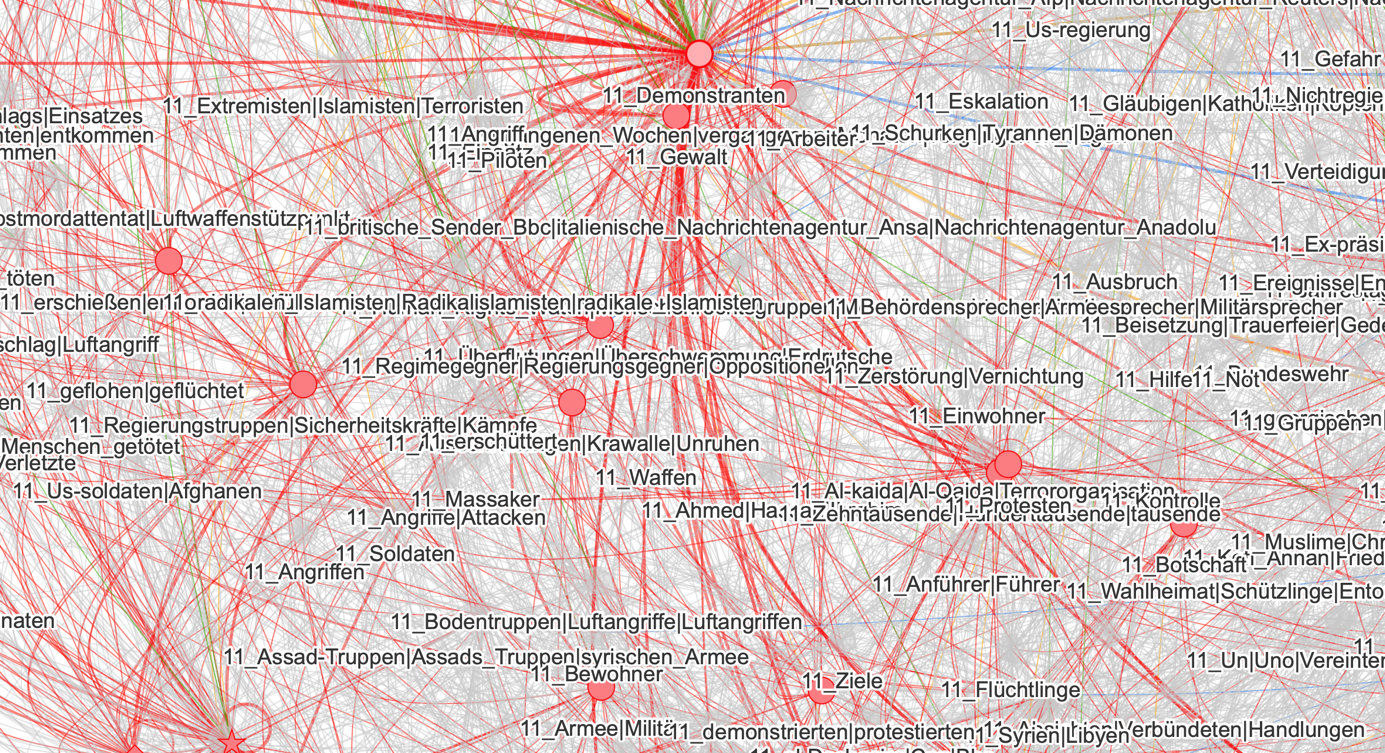
\includegraphics[width=\textwidth]{figures/media/image34.png}
  \caption{\label{fig:islamismus-demonstrationen}Neukonfiguration des Framings von Islamismus bzw. Demonstrationen am Beispiel des FE \cluster{11\_Demonstranten}.}
\end{figure}

Zum Islamismus-Frame sind insbesondere zwei Neukonfigurationen zu nennen: Zum einen schlagen sich die Ereignisse des Arabischen Frühlings deutlich im thematischen Netzwerk-Cluster ‚Krieg \& Islamismus` nieder, sodass nun die auf Demonstrationen bezogenen FE wie \cluster{11\_Protest}, \cluster{11\_Demonstrationen{\breakbar}Kundgebung} oder \cluster{11\_protestieren{\breakbar}demonstrieren}, die zuvor häufig ein eigenes Netzwerk-Cluster bildeten, ein zentraler Teil des thematischen Bereiches ‚Krieg \& Islamismus` werden (\figref{fig:islamismus-demonstrationen}). Zum anderen tritt auch der Bürgerkrieg in Syrien, ebenfalls eine Folge des Arabischen Frühlings, mit FE wie \cluster{11\_syrische\_Opposition{\breakbar}syrische\_Regierung{\breakbar}Präsident\_Assad (politische Akteure Syrienkrieg)}, \cluster{11\_Assads{\breakbar}Präsident\_Baschar\_al-Assad{\breakbar}Regimes (Regime Assad \& Gaddafi)} und \cluster{11\_Assad-Truppen{\breakbar}Assads\_Truppen{\breakbar}syrischen\_Armee (militärische Auseinandersetzungen im Syrienkrieg)} deutlich hervor.

\subsubsection{Fazit}\label{fazit-4}

Im Zeitraum 2011--2013 finden nach einer längeren Phase der Kontinuität größere Umbrüche im Framing einzelner Extremismusvarianten statt. Dabei ist für den Bereich des Rechtsextremismus insbesondere die Wiederkehr eines Framings als gewalttätige, Straftaten begehende Form des Extremismus, wie sie bereits im Zeitraum 1999--2001 vorlag, zu konstatieren. Diese Entwicklung wird durch die Aufdeckung des NSU sowie das Attentat Anders Breiviks ausgelöst und verschiebt den thematischen Fokus der Berichterstattung vom eher abstrakten Bereich eines sozialen, zu bekämpfenden Phänomens in das Netzwerk-Cluster ‚Straftaten \& Juristisches`, was auch eine Replikation der Ergebnisse von Czulo et al. \autocite*{czuloEinflussExtremistischerGewaltereignisse2020} darstellt (siehe \chapref{weitere-arbeiten-zum-extremismusdiskurs-und--begriff}). Die deutliche juristische Prägung ist dabei auch durch den sich über viele Jahre erstreckenden NSU-Prozess sowie das Behördenversagen bei den Ermittlungen zum NSU zu erklären. Auch die juristischen Elemente des Framings der NPD kehren mit dem zweiten NPD-Verbotsverfahren zurück. Der Islamismus-Frame erfährt durch die Ereignisse des Arabischen Frühlings markante Veränderungen. So sind nun Demonstrationen das zentrale, von Bürger*innen ausgeübte Mittel, um gegen die autoritär-islamistischen Regime im Nahen Osten aufzubegehren. Neu zu Tage tritt auch der in Folge des Arabischen Frühlings beginnende Bürgerkrieg in Syrien.

\subsection{Der Zeitraum 2014--2016}\label{der-zeitraum-2014-2016}

\subsubsection{\texorpdfstring{\emph{Corpus-driven} Voranalyse: Thematisch gruppierte Auswahl semantisch äquivalenter Cluster im Vergleich zu den Kern-FE des vorigen Zeitraums}{Corpus-driven Voranalyse: Thematisch gruppierte Auswahl semantisch äquivalenter Cluster im Vergleich zu den Kern-FE des vorigen Zeitraums}}\label{corpus-driven-voranalyse-thematisch-gruppierte-auswahl-semantisch-aequivalenter-cluster-im-vergleich-zu-den-kern-fe-des-vorigen-zeitraums-4}

Die Tabellen \ref{tab:2014_1} und \ref{tab:2014_2} bieten eine Übersicht über die nach Thema gruppierten semantisch äquivalenten Cluster des Zeitraums 2014--2016.

\begin{table}\small
\caption{Thematisch gruppierte Auswahl semantisch äquivalenter Cluster des Zeitraums 2014--2016.}
\label{tab:2014_1}
 \begin{tabularx}{\textwidth}{>{\hsize=0.5\hsize}X >{\hsize=0.5\hsize}X >{\hsize=2.0\hsize}X}
  \lsptoprule
  Extremismus-Variante & Bezug & Frame-Elemente \\
  \midrule
  \multirow{2}{=}{Rechts\-ex\-tre\-mis\-mus} 
  & historisch & \cluster{Holocaust{\breakbar}Nationalsozialismus, Konzentrationslager{\breakbar}Auschwitz-birkenau{\breakbar}Ss, Wehrmacht{\breakbar}Stalin{\breakbar}Roten\_Armee, Auschwitz, Nazis} \\
  & zeit\-ge\-nössisch & \cluster{Neonazis{\breakbar}Rechtsextremisten{\breakbar}Rechtsextreme, Npd, Pegida, Uwe\_Böhnhardt{\breakbar}Uwe\_Mundlos{\breakbar}Böhnhardt, Beate\_Zschäpe{\breakbar}Nsu-prozess, Afd, Frauke\_Petry{\breakbar}Petry{\breakbar}Gauland, Front\_national{\breakbar}Marine\_Le\_Pen{\breakbar}FN, Rassismus{\breakbar}Homophobie{\breakbar}Sexismus, rechtsradikale{\breakbar}rechtsradikalen{\breakbar}rechtsextreme, Heidenau{\breakbar}Freital{\breakbar}Bautzen, Ferguson{\breakbar}Michael\_Brown{\breakbar}Polizeigewalt} \\
  \midrule
  \multirow{2}{=}{Links\-ex\-tre\-mis\-mus} 
  & historisch & \cluster{Ddr} \\
  & zeit\-ge\-nössisch & \cluster{Linke} \\
  \midrule
  \multirow{2}{=}{Politischer Extremismus} 
  & historisch & \cluster{Udssr{\breakbar}Oktoberrevolution{\breakbar}Stalins, Faschisten{\breakbar}Nationalisten{\breakbar}Kommunisten, Weimarer\_Republik{\breakbar}Brd{\breakbar}Ostberlin, Kommunismus{\breakbar}Sozialismus{\breakbar}Diktatur} \\
  & zeit\-ge\-nössisch & \cluster{Antifa{\breakbar}Pegida-Bewegung{\breakbar}Islam-} \\
  \lspbottomrule
 \end{tabularx}
\end{table}

\begin{table}
\caption{Thematisch gruppierte Auswahl semantisch äquivalenter Cluster des Zeitraums 2014--2016.}
\label{tab:2014_2}
 \begin{tabularx}{\textwidth}{>{\hsize=0.5\hsize}X >{\hsize=0.5\hsize}X >{\hsize=2.0\hsize}X}
  \lsptoprule
  Extremismus-Variante & Bezug & Frame-Elemente \\
  \midrule
  {Islamismus} & Nahost\-konflikt & \cluster{Ostjerusalem{\breakbar}Israels\_Armee{\breakbar}radikalislamischen, Hamas, Abbas{\breakbar}Netanjahu{\breakbar}Palästinensern, Gazastreifen{\breakbar}Westjordanland, Jerusalem{\breakbar}Tel\_Aviv{\breakbar}Gaza, israelischen{\breakbar}palästinensische{\breakbar}israelische, Palästinenser{\breakbar}Israelis} \\
  & Syrienkrieg{\slash}Islamischer Staat & \cluster{Baschar\_al-Assad{\breakbar}Machthaber\_Baschar\_al-Assad{\breakbar}Assads, syrischen\_Rebellen{\breakbar}IS-Dschihadisten, Assad, Regime{\breakbar}Assad-regime{\breakbar}militärisch, Al-Nusra-Front{\breakbar}al-Qaida, IS-Miliz{\breakbar}Isis, islamischen\_Staates{\breakbar}iS, kurdische\_Kämpfer{\breakbar}Peschmerga, Kämpfer{\breakbar}Is-kämpfer, Kobane{\breakbar}Mossul{\breakbar}Kobani} \\
  & allgemein & \cluster{Extremisten{\breakbar}Dschihadisten{\breakbar}Islamisten} \\
  \midrule
  varianten\-über\-greifend & Diverses & \cluster{mutmaßlichen\_Terroristen{\breakbar}Abdelhamid\_Abaaoud{\breakbar}Abaaoud} \\
  \lspbottomrule
 \end{tabularx}
\end{table}

\subsubsection{\texorpdfstring{\emph{Corpus-driven} Voranalyse: Cluster mit hoher Cosinus-Distanz im Vergleich zum vorigen Zeitraum}{Corpus-driven Voranalyse: Cluster mit hoher Cosinus-Distanz im Vergleich zum vorigen Zeitraum}}\label{corpus-driven-voranalyse-cluster-mit-hoher-cosinus-distanz-im-vergleich-zum-vorigen-zeitraum-4}

Unter den Ergebnissen (siehe \tabref{tab:cluster-high-cosine-distance-2014}) dieser Voranalyse zeichnen sich als für den Extremismusdiskurs besonders relevant das Erstarken des \cluster{14\_iS}, die sogenannte \cluster{14\_Flüchtlingskrise}, die Kölner \cluster{14\_Silvesternacht} sowie die Ereignisse um die Tötung Michael Browns durch Polizeigewalt in den USA ab.

\begin{table}[t]\small
\caption{Cluster mit hoher Cosinus-Distanz im Vergleich zum vorigen Zeitraum.}
\label{tab:cluster-high-cosine-distance-2014}
\begin{tabularx}{\textwidth}{X r}
\lsptoprule
Cluster & Cos.-Dist. \\
\midrule
\cluster{iS} & 0.93 \\
\cluster{Flüchtlingskrise} & 0.49 \\
\cluster{Krim} & 0.45 \\
\cluster{Ferguson{\breakbar}Michael\_Brown{\breakbar}Polizeigewalt} & 0.43 \\
\cluster{Silvesternacht} & 0.41 \\
\cluster{Minsk} & 0.4 \\
\cluster{Frauke\_Petry{\breakbar}Petry{\breakbar}Gauland} & 0.39 \\
\cluster{Trump{\breakbar}Donald\_Trump} & 0.36 \\
\cluster{Edathy{\breakbar}Hartmann{\breakbar}Ziercke} & 0.36 \\
\cluster{Westafrika} & 0.34 \\
\cluster{Sierra\_Leone{\breakbar}Liberia{\breakbar}Guinea} & 0.31 \\
\cluster{Mariupol{\breakbar}Slowjansk{\breakbar}Luhansk} & 0.31 \\
\cluster{Clinton{\breakbar}Hillary\_Clinton} & 0.31 \\
\cluster{Bundesaußenminister\_Frank-walter\_Steinmeier{\breakbar}Außenminister\_Frank-walter\_Steinmeier} & 0.3 \\
\cluster{Putschversuch{\breakbar}Putsch} & 0.27 \\
\cluster{Heidenau{\breakbar}Freital{\breakbar}Bautzen} & 0.27 \\
\cluster{Flüchtlingspolitik} & 0.27 \\
\cluster{Obergrenze} & 0.23 \\
\cluster{Kobane{\breakbar}Mossul{\breakbar}Kobani} & 0.23 \\
\cluster{Schlepper{\breakbar}Schleuser} & 0.21 \\
\lspbottomrule
\end{tabularx}
\end{table}

\subsubsection{Rechts- und Linksextremismus}\label{rechts--und-linksextremismus-5}

Wie schon zuvor lässt sich aus dem Gesamt-Frame zum politischen Extremismus ein historischer Anteil abgrenzen, der wiederum unterschiedliche Teil-Frames enthält. Darunter ein Frame zur NS-Zeit um die FE \cluster{14\_Holocaust{\breakbar}Nationalsozialismus}, \cluster{14\_Konzentrationslager{\breakbar}Konzentrationslagern{\breakbar}Auschwitz-birkenau}, \cluster{14\_Wehrmacht{\breakbar}Stalin{\breakbar}Roten\_Armee (Akteure NS-Zeit)}, \cluster{14\_Auschwitz} und \cluster{14\_Nazis}; ein Frame zum Totalitarismus bzw. dem 20 Jahrhundert inklusive der Zeit des Kalten Krieges (\cluster{14\_}Udssr{\breakbar}\cluster{Oktoberrevolution{\breakbar}Stalins} (20. Jhdt), \cluster{14\_}Faschisten{\breakbar}\cluster{Nationalisten{\breakbar}Kommunisten} (Anhänger Totalitarismus), \cluster{14\_}Weimarer\cluster{\_Republik{\breakbar}Brd{\breakbar}Ostberlin} (Deutschland 20. Jhdt), \cluster{14\_Kommunismus{\breakbar}Sozialismus{\breakbar}Diktatur (Totalitarismus)}) und letztlich das ausschließlich auf die DDR bezogene FE \cluster{14\_Ddr}. Wie schon in den vorigen Zeiträumen ist das Framing hier insbesondere auf den thematischen Bereich ‚Staat, FdGO \& Gesellschaft` konzentriert, der die Bedrohung dieser Ereignisse für \cluster{14\_Freiheit} und \cluster{14\_Demokratie} deutlich macht und das \cluster{14\_Gedenken} an sie herausstellt. Dabei sind die Ereignisse bzw. Menschen, derer gedacht wird (\cluster{14\_Toten{\breakbar}Todesopfer}, \cluster{14\_Opfer}, \cluster{14\_getöteten{\breakbar}ermordeten{\breakbar}toten}), häufig in einem in diesem Zeitraum neu entstehenden Teil-Frame zu finden, der ‚Tod \& Attentate` thematisiert.\largerpage

Deutlichere Veränderungen, die zu einem großen Teil auf die Fluchtbewegungen der Jahre 2015 und 2016 zurückgehen, finden sich im zeitgenössischen Teil des Rechtsextremismus-Frame. Hier ist zum einen die PEGIDA-Bewegung zu nennen, die -- wie zuvor andere Bewegungen des politischen Extremismus in Deutschland -- insbesondere durch das Agieren im Rahmen von Demonstrationen geframet wird (u.\,a. \cluster{14\_demonstrieren}, \cluster{14\_Aufruf{\breakbar}Appell}, \cluster{14\_Straße}). Durch die Vernetzung mit rechten politischen Akteuren (\cluster{14\_Frauke\_Petry{\breakbar}Petry{\breakbar}Gauland}, \cluster{14\_Npd}) sowie Charakteristika des Rechtsextremismus (\cluster{14\_rechtsradikale{\breakbar}rechtsradikalen{\breakbar}rechtsextreme}, \cluster{14\_Fremdenfeindlichkeit{\breakbar}Intoleranz{\breakbar}Antisemitismus}) wird der rechtsextreme Charakter der Bewegung deutlich. Ein ähnliches Framing, das noch etwas stärker FE zum thematischen Feld des Demonstrierens bindet, zeigt auch das FE \cluster{14\_Antifa{\breakbar}Pegida-Bewegung{\breakbar}Islam}-, das eine breitere Sammlung an Wörtern zur PEGIDA-Bewegung sowie den Protesten und Gegenprotesten enthält (u.\,a. \emph{Aufmärsche}, \emph{linken\_Szene}, \emph{Mob}, \emph{Protestbewegung}, \emph{Pegida-Bewegung}). Mit der Kölner \cluster{14\_Silvesternacht} und der politisch-medial breit geführten Diskussion zu einer \cluster{14\_Obergrenze} hat die \emph{corpus-driven} Voranalyse (\chapref{corpus-driven-voranalyse-cluster-mit-hoher-cosinus-distanz-im-vergleich-zum-vorigen-zeitraum-4}) außerdem zwei Schlagwörter zu Tage gefördert, die für zwei zentrale Diskursereignisse des Zeitraums stehen. Während sich die Diskussion um eine Migrationsobergrenze zwischen den thematischen Frame-Anteilen ‚Flucht \& Migration` sowie ‚Politik` entspannt, wird die Kölner Silvesternacht als juristisch relevantes Ereignis geframet. Dabei changieren die angeschlossenen FE (siehe \figref{fig:silvesternacht-straftaten}) zwischen schweren Straftaten (\cluster{14\_Gewalttaten{\breakbar}Morde{\breakbar}Übergriffe}, \cluster{14\_Straftaten}, \cluster{14\_Täter}) und eher verharmlosenden Begriffen wie \cluster{14\_Vorkommnisse{\breakbar}Verfehlungen{\breakbar}Missstände}.

\begin{figure}[t]
  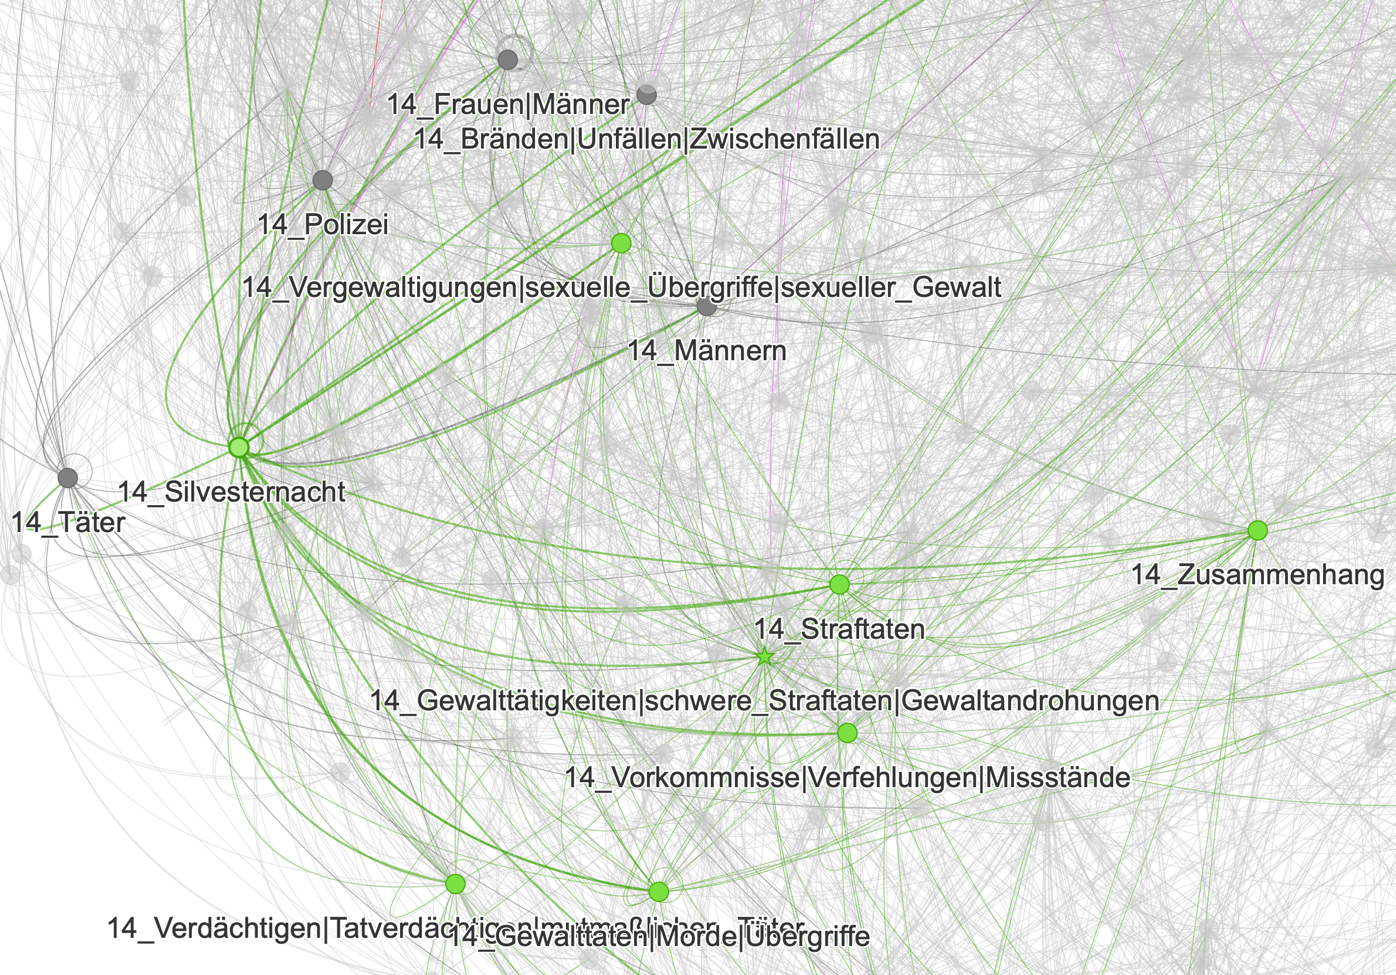
\includegraphics[width=\textwidth]{figures/media/image35.png}
  \caption{\label{fig:silvesternacht-straftaten}Teil der Vernetzung des FE \cluster{14\_Silvesternacht} im Bereich ‚Straftaten \& Juristisches`.}
\end{figure}

Mit dem FE \cluster{14\_Heidenau{\breakbar}Freital{\breakbar}Bautzen} erhalten außerdem einzelne ostdeutsche Orte, an denen rechte Attentate auf Asylunterkünfte verübt wurden, Einzug in den Varianten-Frame. Die verlinkten FE geben dabei Aufschluss über die Art der Anschläge -- aus dem neu entstehenden Migrations-Teil-Frame sind dies etwa \cluster{14\_Flüchtlingsunterkünfte{\breakbar}Flüchtlingsheime{\breakbar}Unterkünfte}, \cluster{14\_Notunterkunft{\breakbar}Erstaufnahmeeinrichtung{\breakbar}Unterkunft} sowie aus dem Cluster um Tod \& Attentate u.\,a. \cluster{14\_Bränden{\breakbar}Unfällen{\breakbar}Zwischenfällen} und \cluster{14\_Brand}. Auch der thematische Bereich ‚Demonstrationen \& politischer Extremismus` leistet eine weitere epistemische Spezifizierung durch die FE \cluster{14\_Ausschreitungen} und \cluster{14\_rechtsradikale{\breakbar}rechtsradikalen{\breakbar}rechtsextreme}. Am angeschlossenen Cluster \cluster{14\_Kanzlerin{\breakbar}Merkel{\breakbar}Angela\_Merkel} lassen sich außerdem Versuche der politischen Auseinandersetzung mit diesen Anschlägen sowie der von rechten Teilen der Bevölkerung gegen die damalige Bundeskanzlerin Merkel gerichtete Hass nachvollziehen (siehe Belege K23--K25 in \tabref{tab:K23-K25}).

\begin{table}
  \caption{Konkordanzen zur Kollokation der Cluster \cluster{14\_Heidenau{\breakbar}Freital{\breakbar}Bautzen} und \cluster{14\_Kanzlerin{\breakbar}Merkel{\breakbar}Angela\_Merkel}.}
  \label{tab:K23-K25}
K23 welt\_3334259
\begin{tabularx}{\textwidth}{QQQ}
\toprule
D-Flüchtlinge-Sachsen-Polizei-Einwanderung-Gewalt-Regierung Merkel nennt Ausschreitungen gegen Flüchtlinge beschämend & {[}14\_Kanzlerin{\breakbar}Merkel{\breakbar}Angela\_Merkel: \emph{\textbf{Kanzlerin}}{]}\newline
\textbf{kritisiert alkoholisierte} \textbf{Schreihälse in}\newline
{[}Heidenau{\breakbar}Freital{\breakbar}Bautzen: \emph{\textbf{Heidenau}}{]} & Bundeskanzlerin\_Angela\_Merkel Cdu hat die wiederholten\_Ausschreitungen an dem Asylbewerberheim im sächsischen\_Heidenau als beschämend kritisiert die Bundeskanzlerin \\
\bottomrule
\end{tabularx}
\bigskip \newline
K24 spiegel\_3335667
\begin{tabularx}{\textwidth}{QQQ}
\toprule
schon leben dass es irgendwann Tote gibt ist angesichts der Gewaltbereitschaft mancher Kreise nicht ausgeschlossen & {[}14\_Kanzlerin{\breakbar}Merkel{\breakbar}Angela\_Merkel: \emph{\textbf{Merkel}}{]}\newline
\textbf{muss in}\newline
{[}Heidenau{\breakbar}Freital{\breakbar}Bautzen: \emph{\textbf{Heidenau}}{]} & spüren dass die Frage wie die Republik mit den Hunderttausenden\_Flüchtlingen umgehen soll mancherorts das Zeug \\
\bottomrule
\end{tabularx}
\bigskip \newline
K25 taz\_3670491
\begin{tabularx}{\textwidth}{QQQ}
\toprule
Bahnhöfen sah man erschöpfte Familien auf dem Schoß abgerissene Kinder fünf Tage zuvor hatten in & {[}Heidenau{\breakbar}Freital{\breakbar}Bautzen: \emph{\textbf{Heidenau}}{]}\newline
\textbf{Fremdenfeinde die}\newline
{[}14\_Kanzlerin{\breakbar}Merkel{\breakbar}Angela\_Merkel: \emph{\textbf{Kanzlerin}}{]} & als Volksverräterin angepöbelt tags\_darauf waren in einem abgestellten Kühllaster auf der österreichischen Autobahn die verwesten\_Leichen \\
\bottomrule
\end{tabularx}
\end{table}

Auch die AfD ist nach ihrem Wandel von einer vordergründig auf wirtschaftliche Themen ausgerichteten Partei zu einer asylkritischen Rechtsaußen-Partei mit den Clustern \cluster{14\_AfD} und \cluster{14\_Frauke\_Petry{\breakbar}Petry{\breakbar}Gauland} im Frame repräsentiert. Neben Frame-Relationen im Bereich der Innenpolitik weist die Partei auch eine starke Verankerung im Bereich ‚Demonstrationen \& politischer Extremismus` auf. Als Partei des äußeren rechten Spektrums wird sie insbesondere durch Anbindungen an rechtxextreme Attribuierungen wie \cluster{14\_Fremdenfeindlichkeit{\breakbar}Intoleranz{\breakbar}Antisemitismus} und \cluster{14\_rechtsradikale{\breakbar}rechtsradikalen{\breakbar}rechtsextreme} epistemisch konturiert. Auch die in Beziehung stehenden politischen Parteien \cluster{14\_Npd}, \cluster{14\_Front\_national{\breakbar}Marine\_Le\_Pen{\breakbar}FN}, die zu Parteien wie \cluster{14\_Union} oder \cluster{14\_Grüne} keine Verbindungen aufweisen, geben Hinweise auf die Stellung im Parteiensystem.

Einen weiteren neuen Akzent markiert in diesem Zeitraum das FE \cluster{14\_Ferguson{\breakbar}Michael\_Brown{\breakbar}Polizeigewalt}, das die Ereignisse um die Tötung Michael Browns durch einen Polizisten im US-amerikanischen Ferguson und die sich anschließenden Debatten und Proteste gegen rassistische Polizeigewalt abbildet. Sichtbar wird dies in FE wie \cluster{14\_Polizei}, \cluster{14\_Schwarze{\breakbar}Schwarzen{\breakbar}Afroamerikaner}, \cluster{14\_Ausschreitungen} oder \cluster{14\_Rassismus{\breakbar}Homophobie{\breakbar}Sexismus}.

\subsubsection{Islamismus}\label{islamismus-5}

Der Islamismus-Frame ist in diesem Zeitraum besonders durch das Erstarken des Islamischen Staates (IS) sowie den damit in Zusammenhang stehenden Syrienkrieg geprägt, was sich in einer Vielzahl von FE im Bereich ‚Krieg \& Islamismus` niederschlägt. Dabei werden sowohl (para\mbox{-})militärische Akteure wie die Cluster \cluster{14\_Kämpfer{\breakbar}Is-kämpfer}, \cluster{14\_syrischen\_Rebellen{\breakbar}syrische\_Rebellen{\breakbar}IS}- und \cluster{14\_kurdische\_Kämpfer{\breakbar}irakischen\_Armee{\breakbar}Pschmerga}; Orte (\cluster{14\_Kobane{\breakbar}Mossul{\breakbar}Kobani}) als auch Terrororganisationen (\cluster{14\_iS}, \cluster{14\_Al-Nusra-Front{\breakbar}Nusra-Front{\breakbar}al-Qaida}) als Teil des Islamismus-Frames offenbar. Die angeschlossenen FE außerhalb des Bereiches ‚Krieg \& Islamismus`framen den IS zu einem großen Teil in seiner Eigenschaft als Organisation, bei der Fragen der Unterstützung bzw. Mitgliedschaft virulent werden: u.\,a. \cluster{14\_Reihen{\breakbar}eigenen\_Reihen}, \cluster{14\_Mitglied}, \cluster{14\_Gruppen{\breakbar}Gruppierungen{\breakbar}Aktionen}, \cluster{14\_Netzwerke{\breakbar}Aktivitäten{\breakbar}Dienste}, \cluster{14\_Gruppe}, \cluster{14\_Anhänger}. Dies hängt auch damit zusammen, dass -- wie bereits zuvor gezeigt -- Fragen der Anhängerschaft von extremistischen Gruppen im Extremismusdiskurs von höchster Bedeutung sind. Dies liegt bei Terrororganisationen wie dem IS neben der gesellschaftlich-ethischen Bedeutung dieses Aspektes auch an der Relevanz für Fragen der inneren Sicherheit und der juristischen Bedeutung, die der Straftatbestand der Mitgliedschaft in einer ausländischen terroristischen Vereinigung hat. Die Konkordanzen K26--K28 in \tabref{tab:K26-K28} illustrieren dies näher.

\begin{table}[t]
  \caption{Konkordanzen zur Kollokation der Cluster \cluster{14\_Mitglied} und \cluster{14\_iS}.}
  \label{tab:K26-K28}
K26 welt\_3668970
\begin{tabularx}{\textwidth}{QQQ}
\toprule
erste islamistische Selbstmordanschlag in Deutschland die Bundesanwaltschaft\_prüft den Verdacht dass der 27-jährige Täter aus Syrien & {[}14\_Mitglied: \textbf{Mitglied}{]}\newline
\textbf{in der Terrormiliz\_islamischer\_Staat}\newline
{[}14\_iS: \textbf{iS}{]} & war wie die Bild unter\_Berufung auf ein psychologisches Fachgutachten berichtet schätzte ein Therapeut aus Lindau \\
\bottomrule
\end{tabularx}
\bigskip \newline
K27 spiegel\_3441101
\begin{tabularx}{\textwidth}{QQQ}
\toprule
zu benennen Ayoub\_B lt100 Jahre\_alt und Ebrahim\_H\_B lt100 Jahre waren nach Überzeugung des Senats beide & {[}14\_Mitglied: \textbf{Mitglied}{]}\newline
\textbf{des}\newline
{[}14\_iS: \textbf{iS}{]} & dass sie Ende Mai 2014 nach\_Syrien\_gereist sind um den Islam zu studieren oder humanitäre\_Hilfe zu \\
\bottomrule
\end{tabularx}
\bigskip \newline
K28 spiegel\_3130133
\begin{tabularx}{\textwidth}{QQQ}
\toprule
hatte der Mann aus Mülheim an der Ruhr ist dringend\_verdächtig sich im vergangenen Sommer als & {[}14\_Mitglied: \textbf{Mitglied}{]}\newline
\textbf{der Terrororganisation\_islamischer\_Staat}\newline
{[}14\_iS: \textbf{iS}{]} & mehrfach an Kampfhandlungen in Syrien beteiligt zu haben er war über Syrien in das Bürgerkriegsland \\
\bottomrule
\end{tabularx}
\end{table}

Im Cluster \cluster{14\_mutmaßlichen\_Terroristen{\breakbar}Abdelhamid\_Abaaoud{\breakbar}Abaaoud (Attentate in Europa)} sind darüber hinaus Wörter zu diversen in Europa verübten Attentaten vereint. Darunter der Anschlag auf dem \emph{Berliner\_Breitscheidplatz} durch \emph{Anis\_Amri}; die Pariser Anschläge von 2015, verübt durch die IS-Mitglieder \emph{Abdelhamid\_Abaaoud}, \emph{Amedy\_Coulibaly} und \emph{Salah\_Abdeslam} und unter Beteiligung von \emph{Najim\_Laachraoui}, der darüber hinaus auch einen Bombenanschlag auf den Brüsseler Flughafen im Jahr 2016 beging; das rechtsextremistisch motivierte Attentat auf Henriette Reker durch \emph{Frank\_S}; das mutmaßlich von \emph{Dschaber al-Bakr} geplante Attentat auf den Berliner Flughafen Tegel; die Anschläge durch \emph{Anders Breivik}, das \emph{NSU-Trio} und weitere. Das Cluster weist eine starke Vernetzung im Frame-Anteil ‚Straftaten \& Juristisches` auf, die durch Ermittlungen und mithin in der Berichterstattung verwendete Ausdrücke der epistemischen Unsicherheit (\cluster{14\_Hinweise}, \cluster{14\_angebliche{\breakbar}angeblichen{\breakbar}vermeintlichen}, \cluster{14\_Bericht\_zufolge}, \cluster{14\_offensichtlich{\breakbar}offenkundig{\breakbar}anscheinend}) geprägt ist. Wissenselemente, die die Taten selbst näher spezifizieren, sind in den Clustern ‚Krieg \& Islamismus` (\cluster{14\_Geiseln}, \cluster{14\_Anschlägen}, \cluster{14\_Anschlag{\breakbar}Attentat{\breakbar}Terroranschlag}) sowie ‚Tod \& Attentate` (\cluster{14\_tötete{\breakbar}erschoss{\breakbar}erschießt}, \cluster{14\_Lastwagen{\breakbar}Lkw}, \cluster{14\_Attacke}) zu finden.

\subsubsection{Fazit}\label{fazit-5}

Im Zeitraum 2014--2016 verändert sich das Framing von Extremismusvarianten erneut deutlich. Bereits in der Makrostruktur des Clusters kristallisieren sich durch die Fluchtbewegungen der Jahre 2015 und 2016 sowie eine Vielzahl von Anschlägen in Europa die Themenfelder ‚Flucht \& Migration` sowie ‚Tod \& Attentate` heraus. Beide Themen stehen in einem inhaltlichen Zusammenhang mit dem Erstarken des IS, das sich im Cluster ‚Krieg \& Islamismus` in einer Vielzahl von FE widerspiegelt. Im Bereich des Rechtsextremismus treten vor diesem Hintergrund mit PEGIDA, der AfD sowie den Brandanschlägen auf Asylunterkünfte neue Akteure und Formen extremistischer Gewalt zu Tage.

\subsection{Der Zeitraum 2017--2019}\label{der-zeitraum-2017-2019}

\subsubsection{\texorpdfstring{\emph{Corpus-driven} Voranalyse: Thematisch gruppierte Auswahl semantisch äquivalenter Cluster im Vergleich zu den Kern-FE des vorigen Zeitraums}{Corpus-driven Voranalyse: Thematisch gruppierte Auswahl semantisch äquivalenter Cluster im Vergleich zu den Kern-FE des vorigen Zeitraums}}\label{corpus-driven-voranalyse-thematisch-gruppierte-auswahl-semantisch-aequivalenter-cluster-im-vergleich-zu-den-kern-fe-des-vorigen-zeitraums-5}

Einen Überblick über die thematisch gruppierte Auswahl semantisch äquivalenter Cluster des Zeitraums 2017--2019 gibt \tabref{tab:2017}.

\begin{table}[t]\small
\caption{Thematisch gruppierte Auswahl semantisch äquivalenter Cluster des Zeitraums 2017--2019.}
\label{tab:2017}
 \begin{tabularx}{\textwidth}{>{\hsize=0.5\hsize}X >{\hsize=0.5\hsize}X >{\hsize=2.0\hsize}X}
  \lsptoprule
  Extremismus-Variante & Bezug & Frame-Elemente \\
  \midrule
  \multirow{2}{=}{Rechts\-ex\-tre\-mis\-mus} 
  & historisch & \cluster{Nationalsozialisten{\breakbar}Holocaust{\breakbar}Nationalsozialismus, Judenverfolgung{\breakbar}Vernichtungslager{\breakbar}Konzentrationslager} \\
  & zeit\-ge\-nössisch & \cluster{Rechtsextremisten{\breakbar}Rechtsextreme{\breakbar}Neonazis, rechtsradikalen{\breakbar}rechtsextremen{\breakbar}rechtsextreme, Gauland{\breakbar}Meuthen{\breakbar}Weidel, Uwe\_Böhnhardt{\breakbar}Böhnhardt{\breakbar}Uwe\_Mundlos, André\_E{\breakbar}Nsu-prozess{\breakbar}Beate\_Zschäpe, Antisemitismus{\breakbar}Rassismus} \\
  \midrule
  \multirow{2}{=}{Links\-ex\-tre\-mis\-mus} 
  & historisch & - \\
  & zeit\-ge\-nössisch & - \\
  \midrule
  \multirow{2}{=}{Politischer Extremismus} 
  & historisch & \cluster{Ddr{\breakbar}Weimarer\_Republik{\breakbar}Sowjetunion, Kommunismus{\breakbar}Sozialismus{\breakbar}Diktatur, Bolschewiki{\breakbar}Kommunisten{\breakbar}kommunistischen} \\
  & zeit\-ge\-nössisch & \cluster{Linkspartei{\breakbar}Afd{\breakbar}Linken, Rechtsradikalen{\breakbar}Rechtsradikale{\breakbar}Rechtsextremen} \\
  \midrule
  {Islamismus} & Nahost\-konflikt & \cluster{Ostjerusalem{\breakbar}Ramallah{\breakbar}Hebron, Gazastreifen{\breakbar}Westjordanland, Hamas, Palästinensern{\breakbar}Israelis} \\
  & Syrienkrieg{\slash}Islamischer Staat & \cluster{Regierungstruppen{\breakbar}Provinz\_Idlib{\breakbar}syrischen\_Armee, Idlib{\breakbar}Afrin{\breakbar}Damaskus, Dschihadisten, Terrormiliz{\breakbar}Terrormiliz\_iS{\breakbar}Terrormiliz\_islamischer\_Staat, Pkk{\breakbar}Terrororganisation{\breakbar}Gülen-bewegung, iS, kurdische{\breakbar}kurdischen{\breakbar}syrische} \\
  & Weiteres & \cluster{Huthi-Rebellen{\breakbar}Huthis{\breakbar}Hisbollah, Amri} \\
  \midrule
  varianten\-über\-greifend & Diverses & \cluster{Rechtsextremismus{\breakbar}Islamismus{\breakbar}Extremismus, rechtsextremistischen{\breakbar}gewaltbereiten{\breakbar}militanten, El\_Paso{\breakbar}Christchurch{\breakbar}Pittsburgh} \\
  \lspbottomrule
 \end{tabularx}
\end{table}

\subsubsection{\texorpdfstring{\emph{Corpus-driven} Voranalyse: Cluster mit hoher Cosinus-Distanz im Vergleich zum vorigen Zeitraum}{Corpus-driven Voranalyse: Cluster mit hoher Cosinus-Distanz im Vergleich zum vorigen Zeitraum}}\label{corpus-driven-voranalyse-cluster-mit-hoher-cosinus-distanz-im-vergleich-zum-vorigen-zeitraum-5}

In diesem Zeitraum prägen außenpolitische Veränderungen, darunter insbesondere die Wahl Donald Trumps zum US-Präsidenten und auch der Brexit, die semantischen Verschiebungen im Vektorraum (siehe \tabref{tab:cluster-high-cosine-distance-2017}). Des Weiteren spiegeln sich als extremismusbezogene Ereignisse rechte Attentate in den USA (\cluster{17\_El\_Paso{\breakbar}Christchruch{\breakbar}Pittsburgh}) und der \emph{G-20-Gipfel} in Hamburg wider.

\begin{table}[t]\small
\caption{Cluster mit hoher Cosinus-Distanz im Vergleich zum vorigen Zeitraum.}
\label{tab:cluster-high-cosine-distance-2017}
\begin{tabularx}{\textwidth}{X r}
\lsptoprule
Cluster & Cos.-Dist. \\
\midrule
\cluster{Dezember\_2016} & 0.62 \\
\cluster{Us-präsident\_Donald\_Trump{\breakbar}Us-präsident\_Trump{\breakbar}Präsident\_Donald\_Trump} & 0.51 \\
\cluster{Puigdemont{\breakbar}Carles\_Puigdemont} & 0.44 \\
\cluster{Mueller{\breakbar}Flynn{\breakbar}Comey} & 0.39 \\
\cluster{G20-gipfel{\breakbar}G-20-Gipfel{\breakbar}beim\_G20-gipfel} & 0.37 \\
\cluster{El\_Paso{\breakbar}Christchurch{\breakbar}Pittsburgh} & 0.36 \\
\cluster{Macron} & 0.35 \\
\cluster{Bolton{\breakbar}Tillerson{\breakbar}Pompeo} & 0.28 \\
\cluster{Kim} & 0.23 \\
\cluster{May{\breakbar}Theresa\_May{\breakbar}Premierministerin\_Theresa\_May} & 0.22 \\
\cluster{Premierministerin\_May{\breakbar}Eu-ratspräsident\_Donald\_Tusk{\breakbar}Eu-kommissionspräsident\_Jean-claude\_Juncker} & 0.21 \\
\cluster{de\_Maizière{\breakbar}De\_Maizière{\breakbar}Pistorius} & 0.2 \\
\cluster{Einzelhaft{\breakbar}Hausarrest{\breakbar}türkischer\_Haft} & 0.2 \\
\cluster{Dekret{\breakbar}Einreiseverbot} & 0.19 \\
\cluster{Wahlbeeinflussung{\breakbar}des\_Trump-Teams{\breakbar}russische\_Hacker} & 0.19 \\
\cluster{Bogotá{\breakbar}Nairobi{\breakbar}Lagos} & 0.17 \\
\cluster{Us-justiz{\breakbar}Missbrauchsvorwürfe{\breakbar}wegen\_sexueller\_Belästigung} & 0.17 \\
\cluster{Trumps{\breakbar}Donald\_Trumps} & 0.17 \\
\cluster{Alan\_Kurdi{\breakbar}Open\_Arms{\breakbar}Aquarius} & 0.17 \\
\cluster{Backstop{\breakbar}Eu-austritt\_Großbritanniens{\breakbar}Austrittsvertrag} & 0.17 \\
\lspbottomrule
\end{tabularx}
\end{table}

\subsubsection{Rechts- und Linksextremismus}\label{rechts--und-linksextremismus-6}

Der Rechtsextremismus-Frame dieses Zeitraumes ist eher durch Kontinuitäten als Brüche im Framing gekennzeichnet. Nach wie vor macht der NSU-Prozess mit den FE \cluster{17\_Uwe\_Böhnhardt{\breakbar}Böhnhardt{\breakbar}Uwe\_Mundlos} und \cluster{17\_André\_E{\breakbar}Nsu-prozess{\breakbar}Beate\_Zschäpe} einen stark juristisch geprägten Anteil aus. Es finden sich nur einzelne Verbindungen in andere thematische Bereiche, so in das Netzwerk-Cluster ‚Tod \& Attentate` (\cluster{17\_erschossen{\breakbar}ermordet}, \cluster{17\_verstorbenen{\breakbar}gestorbenen{\breakbar}Todestag}, \cluster{17\_Opfer{\breakbar}Opfern}), das den NSU-Komplex stärker in Hinblick auf die ermordeten Menschen sowie das Gedenken an sie perspektiviert, und in den Bereich ‚Politischer Extremismus \& Demonstrationen`, der Organisationsaspekte (\cluster{17\_Netzwerk}) sowie den gewalttätig-extremistischen Charakter (\cluster{17\_rechtsextremistischen{\breakbar}gewaltbereiten{\breakbar}militanten}) des NSU einbindet.

Das FE \cluster{17\_Gauland{\breakbar}Meuthen{\breakbar}Weidel (NPD{\slash}AfD-Politiker*innen{\slash}Sahra Wagenknecht)} ist zum einen Teil des Clusters ‚Politik`, zum anderen klar als rechtsextremistisch geframet. Hierzu trägt neben FE aus dem Feld ‚Demonstrationen \& politischer Extremismus` (\cluster{17\_rechtsradikalen{\breakbar}rechtsextremen{\breakbar}rechtsextreme {[}attributive Charakteristika Rechtsextremismus{]}}, \cluster{17\_Rechtsextremismus{\breakbar}Islamismus{\breakbar}Extremismus {[}Extremismusformen{\slash}Radikalisierung{\slash}Fremdenfeindlichkeit{]})} auch das FE \cluster{17\_Verfassungsschutz} bei, das insbesondere für die Beobachtung des ‚Flügels` um Björn Höcke durch den Verfassungsschutz steht.

Die FE \cluster{17\_Rechtsextremisten{\breakbar}Rechtsextreme{\breakbar}Neonazis} und \cluster{17\_rechtsradikalen{\breakbar}rechtsextremen{\breakbar}rechtsextreme (attributive Charakteristika Rechtsextremismus)} versprachlichen Rechtsextremismus zu einem großen Teil explizit. Die an sie angeschlossenen FE sind häufig Objekt der Zuschreibung, rechtsextremistisch zu sein bzw. dem Rechtsextremismus nahe zu stehen. Hierunter fallen einerseits Parteien und Politiker wie in den FE \cluster{17\_Orbán{\breakbar}Viktor\_Orbán{\breakbar}Ungarns}, \cluster{17\_Pd{\breakbar}Podemos{\breakbar}PSOE} oder \cluster{17\_Le\_Pen{\breakbar}Marine\_Le\_Pen{\breakbar}Emmanuel\_Macron}, aber auch die Bundeswehr (\cluster{17\_Bundeswehr}, \cluster{17\_Truppe}), die in Bezug auf rechtextreme Vorfälle zum Gegenstand des medialen Extremismusdiskurses wird (siehe Belege K29--K31 in \tabref{tab:K29-K31}).

\begin{table}[h]\small
  \caption{Konkordanzen zur Kollokation der Cluster \cluster{17\_rechtsradikalen{\breakbar}rechtsextremen{\breakbar}rechtsextreme} und \cluster{17\_Truppe}.}
  \label{tab:K29-K31}
K29 spiegel\_4166845
\begin{tabularx}{\textwidth}{QQQ}
\toprule
sich durch Fehler als Ministerin geschwächt in der Bundeswehr ist sie umstritten seit sie der & {[}17\_Truppe: \textbf{Truppe}{]}\newline
\textbf{nach einzelnen}\newline
{[}17\_rechtsradikalen{\breakbar}rechtsextremen{\breakbar}rechtsextreme: \textbf{rechtsradikalen}{]} & Vorfällen ein Haltungsproblem\_attestiert hat in der Folge kam es zu einem regelrechten Aufstand in der \\
\bottomrule
\end{tabularx}
\bigskip \newline
K30 spiegel\_4272324
\begin{tabularx}{\textwidth}{QQQ}
\toprule
nach einer\_Kleinen\_Anfrage der Grünen-abgeordneten\_Irene\_Mihalic und Konstantin von Notz beide wollten vor\_allem wissen ob sich möglicherweise & {[}17\_rechtsradikalen{\breakbar}rechtsextremen{\breakbar}rechtsextreme: \textbf{rechtsextreme}{]}\newline
\textbf{Soldaten bei der}\newline
{[}17\_Truppe: \textbf{Truppe}{]} & mit Waffen und Munition eingedeckt haben könnten die Antwort ist teilweise kurios so wurden die \\
\bottomrule
\end{tabularx}
\bigskip \newline
K31 welt\_3932906
\begin{tabularx}{\textwidth}{QQQ}
\toprule
konkrete\_Hinweise seien nicht ernst\_genommen worden sagte der Generalinspekteur dem Nachrichtenmagazin stattdessen habe sich in der & {[}17\_Truppe: \textbf{Truppe}{]}\newline
\textbf{gegenüber}\newline
{[}17\_rechtsradikalen{\breakbar}rechtsextremen{\breakbar}rechtsextreme: \textbf{rechtsextremen}{]} & Soldaten ein Muster des Wegsehens etabliert schon 2014 habe es interne Warnsignale gegeben sagte Wieker \\
\bottomrule
\end{tabularx}
\end{table}

Auch das FE \cluster{17\_El\_Paso{\breakbar}Christchurch{\breakbar}Pittsburgh} findet sich unter den verlinkten FE. Es vereint die rechtsextrem motivierten Anschläge von El Paso, Christchurch, Pittsburgh und Charlottesville sowie einen Amoklauf in Parkland und ein islamistisches Attentat in Manchester. Es ist seinerseits im Bereich ‚Demonstrationen \& politischer Extremismus` vernetzt, der die Ereignisse als extremistisch framet. Zudem finden sich Bezüge in den thematischen Bereich ‚Tod \& Anschläge` (u.\,a. \cluster{17\_Attentäter}, \cluster{17\_Todesopfer{\breakbar}Todesopfern{\breakbar}Verletzten}) und Politik (u.\,a. \cluster{17\_Bürgermeister{\breakbar}Oberbürgermeister}, \cluster{17\_Reaktion}, \cluster{17\_Trump{\breakbar}Donald\_Trump{\breakbar}Us-präsident}).

Der Bereich des Linksextremismus ist in diesem Zeitraum kaum in eigenständigen Clustern abgebildet. Lediglich das FE \cluster{17\_G20-gipfel{\breakbar}G-20-Gipfel{\breakbar}beim\_G20-Gipfel} bindet die radikalen linken Proteste (\cluster{17\_Demonstrationen{\breakbar}Kundgebung{\breakbar}Demo}, \cluster{17\_Protest\_gegen{\breakbar}Protest}, \cluster{17\_Demonstrationen{\breakbar}Kundgebungen{\breakbar}Protestte}), bei denen es auch zu Gewalt (\cluster{17\_Gewalt}, \cluster{17\_Ausschreitungen{\breakbar}Krawallen{\breakbar}Krawalle}) und Auseinandersetzungen mit der Polizeit (\cluster{17\_Polizei}, \cluster{17\_Großeinsatz{\breakbar}Polizeieinsatz}, \cluster{17\_Polizisten}) kam, in den Extremismus-Frame dieses Zeitraumes ein.

\subsubsection{Islamismus}\label{islamismus-6}

Neben dem weiterhin präsenten Nahostkonflikt-Frame finden sich im Bereich Islamismus erneut FE, die verstehensrelevantes Wissen um den Krieg in Syrien und den IS kondensieren. Den im engeren Sinne auf kriegerische Handlungen und Orte bezogenen FE aus dem Bereich ‚Krieg \& Islamisimus` wie \cluster{17\_Gebiete{\breakbar}Dörfer}, \cluster{17\_Offensive} oder \cluster{17\_Syrien{\breakbar}Afghanistan} stehen erneut zahlreiche FE wie u.\,a. \cluster{17\_Mitglieder}, \cluster{17\_Mitglied} und \cluster{17\_Verbindungen{\breakbar}Kontakte} zur Seite, sodass der IS in Hinblick auf seine Eigenschaft als Organisation geframet wird. Die Mitgliedschaft stellt dabei -- wie bereits im vorigen Kapitel gezeigt -- einen schweren und auch strafrechtlich relevanten Vorwurf dar.

Nachdem der Anschlag auf den Berliner Breitscheidplatz im zuvor analysieren Zeitraum nur als Teil eines größeren Clusters abgebildet war, was auf den nur wenige Wochen umfassenden Berichtzeitraum im Subkorpus zurückgeht, findet sich nun mit \cluster{17\_Amri} ein FE, das das Attentat klar widerspiegelt. Die Ereignisse des Anschlages werden durch FE wie \cluster{17\_Lastwagen{\breakbar}Lkw}, \cluster{17\_verletzt}, \cluster{17\_Flucht} und \cluster{17\_Anschlag} repräsentiert. Das Framing speist sich darüber hinaus zu großen Anteilen aus dem Bereich ‚Straftaten \& Juristisches`, was auf die Ermittlungen zum Attentat sowie das Behördenversagen im Vorfeld des Anschlages zurückgeht (u.\,a. \cluster{17\_Bka{\breakbar}Lka}, \cluster{17\_Erkenntnisse}, \cluster{17\_Behörden{\breakbar}Sicherheitsbehörden}, \cluster{17\_Geheimdienst{\breakbar}Informanten{\breakbar}Agenten, 17\_Ermittler}), siehe Belege K32--K34 in \tabref{tab:K32-K34}.

\begin{table}[t]
  \caption{Konkordanzen zur Kollokation der Cluster \cluster{17\_Amri} und \cluster{17\_Ermittler}.}
  \label{tab:K32-K34}
K32 spiegel\_4134660
\begin{tabularx}{\textwidth}{QQQ}
\toprule
Prenzlauer\_Berg und häufig in die Fussilet-Moschee Sie wird zu seinem zweiten Zuhause immer\_öfter gelingt es & {[}\cluster{17\_Amri}: \textbf{Amri}{]}\newline
\textbf{die}\newline
{[}\cluster{17\_Ermittler}: \textbf{Ermittler}{]} & abzuschütteln an der Turmstraße springt er im letzten Moment in die vollbesetzte U-bahn die Zielperson \\
\bottomrule
\end{tabularx}
\bigskip \newline
K33 welt\_4134954
\begin{tabularx}{\textwidth}{QQQ}
\toprule
Jahr 2016 mit dem Tunesier und der Gefahr die von ihm ausging die Einschätzung der & {[}\cluster{17\_Ermittler}: \textbf{Ermittler}{]}\newline
\textbf{damals}\newline
{[}\cluster{17\_Amri}: \textbf{Amri}{]} & war definitiv gefährlich aber von ihm ging keine\_akute\_Gefahr aus solch eine fatale\_Fehleinschätzung soll es in \\
\bottomrule
\end{tabularx}
\bigskip \newline
K34 spiegel\_4113989
\begin{tabularx}{\textwidth}{QQQ}
\toprule
Berlin-Attentäter Amri-Ermittler übersahen Handyfotos mit Waffen Neue Panne im Fall des Berliner\_Attentäters\_Anis & {[}\cluster{17\_Amri}: \textbf{Amri}{]}\newline
\newline
{[}\cluster{17\_Ermittler}: \textbf{Ermittler}{]} & haben ein Handy des späteren Terroristen nur oberflächlich ausgewertet im Fall\_Anis\_Amri hat es eine weitere \\
\bottomrule
\end{tabularx}
\end{table}

Auch das verknüpfte FE \cluster{17\_Gefährder{\breakbar}Straftäter} ist in diesem Zusammenhang Teil des verstehensrelevanten Wissens. Zum einen findet sich hier mit dem Wort \emph{Gefährder} ein Begriff, der von Sicherheitsbehörden im Kontext Extremismus verwendet wird, um Personen zu bezeichnen, die im Verdacht stehen, schwere extremistisch motivierte Straftaten, wie z.\,B. Attentate, zu planen.\footnote{Wie im Extremismusdiskurs häufig der Fall, handelt es sich dabei nicht um einen Rechtsbegriff, sondern um polizeilich-institutionelles Vokabular, dessen Anwendung auf ein Individuum jedoch z.\,B. zu erweiterten Ermittlungsbefugnissen führen kann (siehe \url{https://www.bpb.de/themen/migration-integration/kurzdossiers/migration-und-sicherheit/302982/gefaehrder/}).} Wie die Konkordanzen K35--K37 in \tabref{tab:K35-K37} zeigen, bestehen zwischen den im Amri-Frame gleichzeitig auftretenden FE zum Anschlag einerseits und dem Gefährder-Status andererseits ein \emph{constraint}, der ein gleichzeitiges Auftreten eigentlich nicht vorsieht: Wer von den Sicherheitsbehörden beobachtet wird, weil er im Verdacht steht, einen Anschlag zu begehen, kann dazu keine Gelegenheit haben. Dass dies trotzdem geschehen ist, macht die explizite Auseinandersetzung notwendig.

\begin{table}[t]
  \caption{Konkordanzen zur Kollokation der Cluster \cluster{17\_Amri} und \cluster{17\_Gefährder{\breakbar}Straftäter}.}
  \label{tab:K35-K37}
K35 spiegel\_4218285
\begin{tabularx}{\textwidth}{QQQ}
\toprule
von der Spd-geführten Düsseldorfer\_Innenministerium dabei ging es vor\_allem um die politisch\_brisante Frage warum der als & {[}\cluster{17\_Gefährder{\breakbar}Straftäter}: \textbf{Gefährder}{]}\newline
\textbf{und potenzieller\_Terrorist eingestufte\_Tunesier}\newline
{[}\cluster{17\_Amri}: \textbf{Amri}{]} & nicht längst außer\_Landes geschafft worden war die Antwort der Ministerialen lautete verkürzt gesagt weil Tunesien \\
\bottomrule
\end{tabularx}
\bigskip \newline
K36 welt\_4131731
\begin{tabularx}{\textwidth}{QQQ}
\toprule
Polizisten\_erschossen worden in dem Fall gab es eine ganze Serie von schweren Pannen und Ermittlungsfehlern & {[}\cluster{17\_Amri}: \textbf{Amri}{]}\newline
\textbf{war ein bekannter\_Islamist}\newline
{[}\cluster{17\_Gefährder{\breakbar}Straftäter}: \textbf{Gefährder}{]} & und verurteilter\_Straftäter der eigentlich hätte abgeschoben werden sollen aber stattdessen mit diversen Identitäten umherzog die \\
\bottomrule
\end{tabularx}
\bigskip \newline
K37 taz\_4523740
\begin{tabularx}{\textwidth}{QQQ}
\toprule
drangen Sie fragen sich ob da möglicherweise etwas vertuscht werden soll etwa dass man die & {[}\cluster{17\_Gefährder{\breakbar}Straftäter}: \textbf{Gefährder}{]}\newline
\newline
{[}\cluster{17\_Amri}: \textbf{Amri}{]} & und Ba nicht von der Straße holte weil man sich von ihnen interessante Informationen über \\
\bottomrule
\end{tabularx}
\end{table}

\subsubsection{Fazit}\label{fazit-6}

Insgesamt ist der Zeitraum 2017--2019 durch wiederkehrende Framing-Mechanis\-men geprägt. Wie schon zuvor der NSU wird auch der Anschlag durch Anis Amri zu einem wesentlichen Teil in Hinblick auf die juristische Aufarbeitung bzw. das Versagen der Sicherheitsbehörden geframet. Es zeigen sich dabei Spannungen innerhalb des Frames durch das gemeinsame Auftreten von \emph{constraints} unterliegenden FE. Im Bereich des politischen Extremismus tritt im linken Spektrum der G-20-Gipfel zu Tage, wobei sich das gewaltbezogene Framing (\cluster{17\_Ausschreitungen{\breakbar}Krawallen{\breakbar}Krawalle}, \cluster{17\_Gewalt}) im Vergleich zum G-8-Gipfel in Heiligendamm im Zeitraum 2005--2007 intensiviert hat, sich jedoch deutlich von rechten oder islamistischen Gewaltereignissen unterscheidet. Am Beispiel des FE \cluster{17\_El\_Paso{\breakbar}Christchurch{\breakbar}Pittsburgh} betrifft dies sowohl die die Taten selbst betreffenden Ausdrücke bzw. FE wie \cluster{17\_Todesopfer{\breakbar}Todesopfern{\breakbar}Verletzten} oder \cluster{17\_Messerattacke{\breakbar}Messerangriff{\breakbar}Schüssen} als auch die Einordnung der extremistischen Gewaltereignisse in Hinblick auf ihre Schwere, etwa als \cluster{17\_Attentat{\breakbar}Terroranschlag} oder \cluster{17\_Terrorismus{\breakbar}Terror}.

\subsection{Der Zeitraum 2020 -- August 2021}\label{der-zeitraum-2020-august-2021}

\subsubsection{\texorpdfstring{\emph{Corpus-driven} Voranalyse: Thematisch gruppierte Auswahl semantisch äquivalenter Cluster im Vergleich zu den Kern-FE des vorigen Zeitraums}{Corpus-driven Voranalyse: Thematisch gruppierte Auswahl semantisch äquivalenter Cluster im Vergleich zu den Kern-FE des vorigen Zeitraums}}\label{corpus-driven-voranalyse-thematisch-gruppierte-auswahl-semantisch-aequivalenter-cluster-im-vergleich-zu-den-kern-fe-des-vorigen-zeitraums-6}

\tabref{tab:2020} zeigt die thematisch gruppierte Auswahl semantisch äquivalenter Cluster des Zeitraums 2020--2021.

\begin{table}\footnotesize
\caption{Thematisch gruppierte Auswahl semantisch äquivalenter Cluster des Zeitraums 2020--2021.}
\label{tab:2020}
 \begin{tabularx}{\textwidth}{>{\hsize=0.5\hsize}X >{\hsize=0.5\hsize}X >{\hsize=2.0\hsize}X}
  \lsptoprule
  Extremismus-Variante & Bezug & Frame-Elemente \\
  \midrule
  \multirow{2}{=}{Rechts\-ex\-tre\-mis\-mus}
  & historisch & \cluster{Nationalsozialismus{\breakbar}Holocaust, Nazis} \\
  & zeit\-ge\-nössisch & \cluster{Rechtsextremen{\breakbar}Rechtsextremisten{\breakbar}Neonazis, rechtsextremen{\breakbar}antisemitische{\breakbar}rechtsextreme, Höcke{\breakbar}Kalbitz{\breakbar}Andreas\_Kalbitz, Afd{\breakbar}Partei, Stephan\_Ernst{\breakbar}Markus\_H{\breakbar}Mittäter, Antisemitismus{\breakbar}Rassismus{\breakbar}Rechtsextremismus, George\_Floyd{\breakbar}Floyd{\breakbar}des\_Afroamerikaners\_George, Portland{\breakbar}Minneapolis{\breakbar}Nationalgarde, Hanau} \\
  \midrule
  \multirow{2}{=}{Links\-ex\-tre\-mis\-mus}
  & historisch & - \\
  & zeit\-ge\-nössisch & - \\
  \midrule
  \multirow{2}{=}{Politischer Extremismus}
  & historisch & \cluster{Mai\_1945{\breakbar}Stalin{\breakbar}Hitlers, 1945{\breakbar}1939{\breakbar}1944} \\
  & zeit\-ge\-nössisch & \cluster{Susanne\_Hennig-Wellsow{\breakbar}Hennig-Wellsow{\breakbar}Mike\_Mohring} \\
  \midrule
  Islamismus  & Nahost\-konflikt & \cluster{Gaza{\breakbar}Hamas{\breakbar}Jerusalem} \\
  & Syrienkrieg{\slash}Islamischer Staat & \cluster{Syrien{\breakbar}Afghanistan{\breakbar}Libyen, iS{\breakbar}Islamisten{\breakbar}Terrormiliz\_islamischer\_Staat} \\
  & Afghanistan & \cluster{Taliban} \\
  \lspbottomrule
 \end{tabularx}
\end{table}

\subsubsection{\texorpdfstring{\emph{Corpus-driven} Voranalyse: Cluster mit hoher Cosinus-Distanz im Vergleich zum vorigen Zeitraum}{Corpus-driven Voranalyse: Cluster mit hoher Cosinus-Distanz im Vergleich zum vorigen Zeitraum}}\label{corpus-driven-voranalyse-cluster-mit-hoher-cosinus-distanz-im-vergleich-zum-vorigen-zeitraum-6}

Die Übersicht der datengeleitet identifizierten Cluster mit der höchsten Cosinus-Distanz wird in diesem Zeitraum stark durch die Corona-Pandemie bestimmt (siehe \tabref{tab:cluster-high-cosine-distance-2020}). An erster Stelle schlägt sich mit \cluster{20\_Hanau} jedoch ein extremistisches Gewaltereignis nieder.

\begin{table}[h]\small
\caption{Cluster mit hoher Cosinus-Distanz im Vergleich zum vorigen Zeitraum.}
\label{tab:cluster-high-cosine-distance-2020}
\begin{tabularx}{\textwidth}{X r}
\lsptoprule
Cluster & Cos.-Dist. \\
\midrule
\cluster{Hanau} & 0.57 \\
\cluster{Corona-Schutzmaßnahmen{\breakbar}Corona-Beschränkungen{\breakbar}Ausgangsbeschränkungen} & 0.41 \\
\cluster{Belarus{\breakbar}Minsk} & 0.34 \\
\cluster{Infizierte{\breakbar}Infizierten{\breakbar}Menschen\_starben} & 0.29 \\
\cluster{Portland{\breakbar}Minneapolis{\breakbar}Nationalgarde} & 0.28 \\
\cluster{Wirecard} & 0.23 \\
\cluster{Einreisebeschränkungen{\breakbar}Reisewarnungen{\breakbar}Reisebeschränkungen} & 0.23 \\
\cluster{Joe\_Biden{\breakbar}Biden{\breakbar}Donald\_Trump} & 0.21 \\
\cluster{Ausbreitung{\breakbar}Verbreitung} & 0.19 \\
\cluster{Bergkarabach{\breakbar}Armenien{\breakbar}Aserbaidschan} & 0.19 \\
\cluster{Taiwan{\breakbar}Peking{\breakbar}Südkorea} & 0.18 \\
\cluster{Ministerpräsidenten} & 0.18 \\
\cluster{Ausbruch} & 0.18 \\
\cluster{Einstufung} & 0.18 \\
\cluster{South\_Carolina{\breakbar}Arizona{\breakbar}Wisconsin} & 0.16 \\
\cluster{Mike\_Pence{\breakbar}oppositionellen\_Demokraten{\breakbar}republikanische} & 0.15 \\
\cluster{Pence{\breakbar}McConnell{\breakbar}Vizepräsident\_Mike\_Pence} & 0.15 \\
\cluster{gehandelt} & 0.15 \\
\cluster{Kontakte{\breakbar}Verbindungen} & 0.15 \\
\cluster{Mosambik{\breakbar}Angola{\breakbar}Honduras} & 0.15 \\
\lspbottomrule
\end{tabularx}
\end{table}

\subsubsection{Rechts- und Linksextremismus}\label{rechts--und-linksextremismus-7}

\largerpage
Für den Bereich des politischen Extremismus erscheinen in diesem Zeitraum insbesondere die zeitgenössischen Teile des Frames von Veränderungen geprägt zu sein, wobei keine dezidiert für den Linksextremismus einschlägigen Cluster zu Tage treten. Politische Akteure fast aller Parteien finden sich im FE \cluster{20\_Susanne\_Hennig-Wellsow{\breakbar}Hennig-Wellsow{\breakbar}Mike\_Mohring}, das hier Berücksichtigung findet, da es einerseits im Rahmen der Analyse semantisch äquivalenter Cluster (siehe Tabelle 9 im Anhang) auffiel und andererseits mit \emph{Susanne\_Hennig-Welsow}, \emph{Mike\_Mohring}, \emph{Bodo\_Ramelow}, \emph{Thomas\_Kämmerich} und \emph{Thüringer\_Ministerpräsidenten} Ausdrücke enthält, die auf die Ereignisse um die Wahl Thomas Kämmerichs zum Thüringischen Ministerpräsidenten mit Stimmen der AfD referieren. Diese Ereignisse spiegeln sich auch in angeschlossenen FE wie \cluster{20\_AfD{\breakbar}Partei}, \cluster{20\_Ministerpräsident{\breakbar}Regierungschef} oder \cluster{20\_Rücktritt} wider, wobei sich das Framing fast ausschließlich im Bereich des Clusters ‚Politik` abspielt und die FE, die den Vorgang deutlicher als für den Extremismusdiskurs relevant rahmen, nur indirekt angeschlossen sind, etwa an das FE \cluster{20\_AfD{\breakbar}Politik}. Für die AfD, die neben jenem Cluster auch in einem gesonderten, einige Politiker sowie Parteistrukturen umfassenden FE (\cluster{20\_Höcke{\breakbar}Kalbitz{\breakbar}Andreas\_Kalbitz}) abgebildet ist, ist ein Framing zu konstatieren, das innerparteiliche Konflikte (u.\,a. \cluster{20\_Seite}, \cluster{20\_Gegner,} \cluster{20\_Konflikt{\breakbar}Kampf{\breakbar}Machtkampf}) sowie die Einstufung des sogenannten ‚Flügels` als gesichert rechtsextrem durch den Verfassungsschutz und die darauf folgende Auflösung der Parteistruktur (u.\,a. \cluster{20\_Verfassungsschutz}, \cluster{20\_Einstufung}, \cluster{20\_rechtsextremen{\breakbar}antisemitische{\breakbar}rechtsextreme}) deutlich macht.

Im FE \cluster{20\_Stephan\_Ernst{\breakbar}Markus\_H{\breakbar}Mittäter} sind darüber hinaus Ausdrücke organisiert, die auf rechte Attentate Bezug nehmen, insbesondere auf den Mord an Walter Lübcke (u.\,a. \emph{Stephan\_Ernst}, \emph{Markus\_H}, \emph{Walter\_Lübcke}), aber auch auf Ermittlungen bzw. Gerichtsverfahren generell (u.\,a. \emph{mutmaßlich}, \emph{Motiv}, \emph{laut\_Anklage}). Seine Verbindungen im Frame sind, wie bereits bei anderen in Deutschland verübten Attentaten, insbesondere im Netzwerk-Cluster ‚Straftaten \& Juristisches` angelegt, erstrecken sich jedoch auch in den hier neu auftretenden thematischen Teil-Frame ‚Anschläge, Gedenken \& Nationalsozialismus`, wo sich die Benennung als \emph{Attentat} (\cluster{20\_Attentat{\breakbar}Terroranschlag{\breakbar}Anschläge}) und die rechtsextremistisch motivierten Anschläge in Hanau (\cluster{20\_Hanau}) und Halle (\cluster{20\_Synagoge}) wiederfinden. Auch diese Anschläge weisen ein in weiten Teilen ähnliches Framing auf, wobei der Anschlag in Hanau etwas stärker in Hinblick auf die Trauer der Angehörigen-Familien und das Gedenken an die Opfer perspektiviert wird (\cluster{20\_Gedenkfeier{\breakbar}Gedenkveranstaltung{\breakbar}Trauerfeier}, \cluster{20\_Schmerz{\breakbar}Trauer{\breakbar}Scham}, \cluster{20\_Angehörigen{\breakbar}Angehörige}, \cluster{20\_Familien}). Die Konkordanzen K38--K40 in \tabref{tab:K38-K40} illustrieren dies exemplarisch.

\begin{table}[t]
  \caption{Konkordanzen zur Kollokation der Cluster \cluster{20\_Hanau} und \cluster{20\_Schmerz{\breakbar}Trauer{\breakbar}Scham}.}
  \label{tab:K38-K40}
K38 taz\_4862583
\begin{tabularx}{\textwidth}{QQQ}
\toprule
manche geben der Afd eine Mitschuld Stuttgart\_dpalsw - der mutmaßlich rechtsradikale und rassistische Anschlag von & {[}\cluster{20\_Hanau}: \textbf{Hanau}{]}\newline
\textbf{hat in Baden-württemberg Bestürzung und}\newline
{[}\cluster{20\_Schmerz{\breakbar}Trauer{\breakbar}Scham}: \textbf{Trauer}{]} & ausgelöst der Landtag von Baden-württemberg ist tief\_erschüttert von den rassistisch\_motivierten\_Morden in Hanau teilte Landtagspräsidentin\_Muhterem\_Aras Grüne \\
\bottomrule
\end{tabularx}
\bigskip \newline
K39 spiegel\_4851116
\begin{tabularx}{\textwidth}{QQQ}
\toprule
nicht nachlassen für das friedliche\_Miteinander in unserem\_Land einzustehen Außenminister\_Heiko\_Maas drückt den Angehörigen der Opfer sein & {[}\cluster{20\_Schmerz{\breakbar}Trauer{\breakbar}Scham}: \textbf{Mitgefühl}{]}\newline
\textbf{aus die schrecklichen\_Ereignisse in}\newline
{[}\cluster{20\_Hanau}: \textbf{Hanau}{]} & schmerzen uns alle twittert der Spd-politiker nach dieser grausamen Nacht sind unsere Gedanken bei den \\
\bottomrule
\end{tabularx}
\bigskip \newline
K40 welt\_5115165
\begin{tabularx}{\textwidth}{QQQ}
\toprule
Menschen demütigen bedrohen jagen oder gar ermorden Lübckes Familie übermittelte den Hinterbliebenen der Opfer von & {[}\cluster{20\_Hanau}: \textbf{Hanau}{]}\newline
\textbf{am\_Freitag ihr}\newline
{[}\cluster{20\_Schmerz{\breakbar}Trauer{\breakbar}Scham}: \textbf{Mitgefühl}{]} & es bleibe aber nicht nur Schmerz sondern es gebe auch viele drängende\_Fragen erklärte sie und \\
\bottomrule
\end{tabularx}
\end{table}

\begin{figure}
  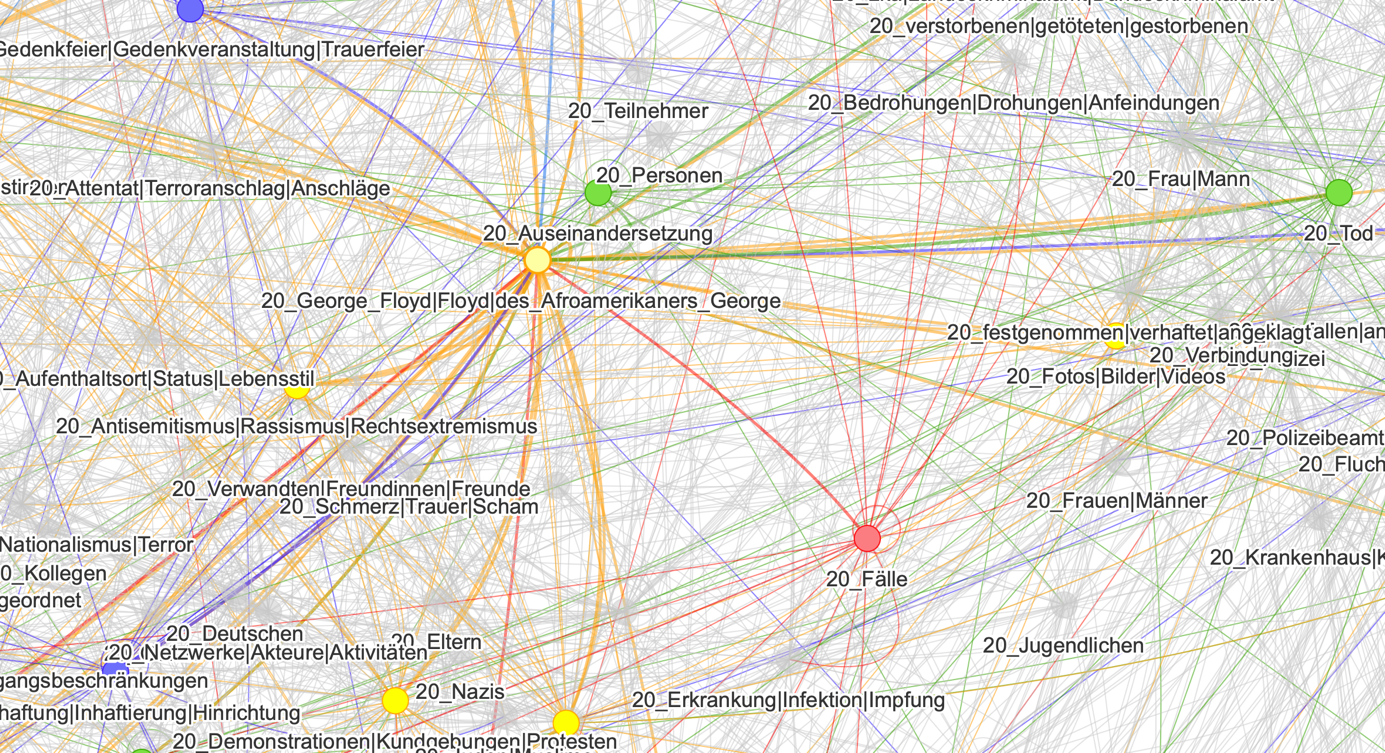
\includegraphics[width=\textwidth]{figures/media/image36.png}
  \caption{\label{fig:george-floyd-frame}Teil des George-Floyd-Frames.}
\end{figure}

Des Weiteren wird mit dem FE \cluster{20\_George\_Floyd{\breakbar}Floyd{\breakbar}des\_Afroamerikaners\_George} erneut ein Fall von in den USA gegen Schwarze ausgeübter Polizeigewalt emergent (siehe \figref{fig:george-floyd-frame}). Auch die sich anschließenden \emph{Black-Lives-Matter}-Proteste finden sich wieder. Zum einen im unten noch näher analysierten FE \cluster{20\_Extinction\_Rebellion{\breakbar}Fridays\_for\_Future{\breakbar}aktivistInnen}, zum anderen im Cluster \cluster{20\_Portland{\breakbar}Minneapolis{\breakbar}Nationalgarde}, das einzelne Orte der Proteste sowie die \emph{Nationalgarde} enthält, die in Teilen des Landes eingesetzt wurde, um gegen die Proteste vorzugehen.

Einzelne Akteure des Rechtsextremismus finden sich zudem im FE \cluster{20\_Rechtsextremen{\breakbar}Rechtsextremisten{\breakbar}Neonazis}, wobei auch eine linke Organisation (\emph{Antifa}) sowie die im Rahmen der Corona-Pandemie neu entstehende Querdenken-Bewegung (\emph{Querdenker}) hier enthalten sind. Über die Vernetzung mit anderen FE wird Rechtsextremismus als (zum Teil politisch) organisiertes Phänomen (\cluster{20\_AfD{\breakbar}Partei}, \cluster{20\_Höcke{\breakbar}Kalbitz{\breakbar}Andreas\_Kalbitz}, \cluster{20\_Gruppen, 20\_Mitglieder}) konstruiert, dessen Handlungsspektrum auf Demonstrationen (u.\,a. \cluster{20\_Demonstrationen{\breakbar}Kundgebung{\breakbar}Demo}, \cluster{20\_protestieren{\breakbar}protestierten{\breakbar}demonstrieren}) fokussiert ist, jedoch auch schwere Gewalttaten (\cluster{20\_Attentat{\breakbar}Terroranschlag{\breakbar}Anschläge}, \cluster{20\_Bedrohungen{\breakbar}Drohungen{\breakbar}Anfeindungen {[}hier auch u.\,a. enthalten: \emph{Attacken}, \emph{Übergriffe}, \emph{Gewalttaten}{]})} umfasst.

Am FE \cluster{20\_Antisemitismus{\breakbar}Rassismus{\breakbar}Rechtsextremismus (Kennzeichen des Rechtsextremismus{\slash}Rechtsextremismus)} zeigt sich erneut der Stigmacharakter des Extremismuskonzeptes (\cluster{20\_Vorwurf}, \cluster{20\_vorgeworfen}). Auch Sicherheitsbehörden wie die \cluster{20\_Polizei} werden wieder als Träger rechtsextremistischer Merkmale diskutiert (siehe Belege K41--K43 in \tabref{tab:K41-K43}).

\begin{table}[t]
  \caption{Konkordanzen zur Kollokation der Cluster \cluster{20\_Antisemitismus{\breakbar}Rassismus{\breakbar}Rechtsextremismus} und \cluster{20\_Polizei}.}
  \label{tab:K41-K43}
K41 taz\_4934582
\begin{tabularx}{\textwidth}{QQQ}
\toprule
Debatte über & {[}\cluster{20\_Antisemitismus{\breakbar}Rassismus{\breakbar}Rechtsextremismus}: \textbf{Rassismus}{]}\newline
\textbf{in}\newline
{[}\cluster{20\_Polizei}: \textbf{Polizei}{]} & wissen wir seit den NSU-Morden Spd-chefin\_Saskia\_Esken wird für ihren Satz unter Polizistinnen in Deutschland gebe \\
\bottomrule
\end{tabularx}
\bigskip \newline
K42 taz\_4952496
\begin{tabularx}{\textwidth}{QQQ}
\toprule
Polizeisprecher über Rassimus wir nehmen keine Hautfarbe fest Thilo\_Cablitz weiß dass es auch bei der & {[}\cluster{20\_Polizei}: \textbf{Polizei}{]}\newline
\newline
{[}\cluster{20\_Antisemitismus{\breakbar}Rassismus{\breakbar}Rechtsextremismus}: \textbf{Rassismus}{]} & gibt aber das sei keinesfalls die Regel sagt der Chef der Pressestelle der Polizei Berlin \\
\bottomrule
\end{tabularx}
\bigskip \newline
K43 taz\_5230564
\begin{tabularx}{\textwidth}{QQQ}
\toprule
die Rede von der kritischen Unabhängigkeit immer mehr zur Farce wird ausgerechnet ein Buch das & {[}\cluster{20\_Antisemitismus{\breakbar}Rassismus{\breakbar}Rechtsextremismus}: \textbf{Rechtsextremismus}{]}\newline
\textbf{in} \textbf{der}\newline
{[}\cluster{20\_Polizei}: \textbf{Polizei}{]} & adressiert denn nachdem das BMI der bpb letzthin eine Links­extremismusdefinition des Verfassungsschutzes diktiert hat hat \\
\bottomrule
\end{tabularx}
\end{table}

Auch warum eher unerwartet das FE \cluster{20\_Meghan{\breakbar}Prinz\_Harry{\breakbar}Harry} hier als Teil des Extremismusdiskurses aufscheint, wird durch die Anbindung an Charakteristika des Rechtsextremismus deutlich. So warfen Prinz Harry und seine Frau Meghan Markle der britischen Königsfamilie Rassismus vor (siehe Belege K44--K46 in \tabref{tab:K44-K46}).

\begin{table}
  \caption{Konkordanzen zur Kollokation der Cluster \cluster{20\_Meghan{\breakbar}Prinz\_Harry{\breakbar}Harry} und \cluster{20\_Antisemitismus{\breakbar}Rassismus{\breakbar}Rechtsextremismus}.}
  \label{tab:K44-K46}
K44 spiegel\_5184036
\begin{tabularx}{\textwidth}{QQQ}
\toprule
erhoben sie im März schwere\_Vorwürfe\_gegen das Königshaus von dem sie sich nicht ausreichend unterstützt fühlten & {[}\cluster{20\_Meghan{\breakbar}Prinz\_Harry{\breakbar}Harry}: \textbf{Meghan}{]}\newline
\textbf{beklagte zudem}\newline
{[}\cluster{20\_Antisemitismus{\breakbar}Rassismus{\breakbar}Rechtsextremismus}: \textbf{Rassismus}{]} & im britischen\_Königshaus seitdem gilt das Verhältnis\_zwischen den beiden und dem Rest der Royals als noch \\
\bottomrule
\end{tabularx}
\bigskip \newline
K45 spiegel\_5130368
\begin{tabularx}{\textwidth}{QQQ}
\toprule
Harry wir sind keine rassistische Familie Prinz\_William verteidigt den britischen Palast gegen den Vorwurf des & {[}\cluster{20\_Antisemitismus{\breakbar}Rassismus{\breakbar}Rechtsextremismus}: \textbf{Rassismus}{]}\newline
\textbf{den}\newline
{[}\cluster{20\_Meghan{\breakbar}Prinz\_Harry{\breakbar}Harry}: \textbf{Meghan}{]} & und Harry erhoben hatten ein Gespräch der Brüder über das Thema steht aber offenbar noch \\
\bottomrule
\end{tabularx}
\bigskip \newline
K46 welt\_5208098
\begin{tabularx}{\textwidth}{QQQ}
\toprule
Kinder in einem Aufsehen\_erregenden Interview mit US-Talkshowlegende Oprah\_Winfrey warfen sie dem Königshaus mangelnde\_Rücksichtnahme und sogar & {[}\cluster{20\_Antisemitismus{\breakbar}Rassismus{\breakbar}Rechtsextremismus}: \textbf{Rassismus}{]}\newline
\textbf{vor}\newline
{[}\cluster{20\_Meghan{\breakbar}Prinz\_Harry{\breakbar}Harry}: \textbf{Meghan}{]} & lt100 hat teilweise afroamerikanische\_Wurzeln der Sunken Garden soll eine besondere\_Anziehungskraft auf die Prinzessin ausgeübt haben \\
\bottomrule
\end{tabularx}
\end{table}

Als letztes FE soll mit \cluster{20\_Extinction\_Rebellion{\breakbar}Fridays\_for\_Future{\breakbar}aktivistInnen} ein Cluster in den Blick genommen werden, das unterschiedliche demonstrierende Gruppen umfasst (u.\,a. \emph{Fridays\_for\_Future}, \emph{Extinction\_Rebellion}, \emph{Black\_Lives\_Matter}, \emph{Querdenken}, \emph{Greenpeace}, \emph{Klimabewegung}), die nicht als extremistisch gelten und sich auch nicht ohne Weiteres in die Extremismus-Trias aus Links- und Rechtsextremismus sowie Islamismus einordnen lassen. Die paradigmatische Ähnlichkeit, die das Zu-Tage-Treten im Frame bedingt, liegt in der Organisiertheit (\cluster{20\_Gruppen}, \cluster{20\_Netzwerke, 20\_Organisationen{\breakbar}Initiativen{\breakbar}Stiftungen}, \cluster{20\_Netzwerke{\breakbar}Akteure{\breakbar}Aktivitäten}) und dem außerparlamentarischen Agieren in Form von Protesten und Demonstrationen (u.\,a. \cluster{20\_Widerstand{\breakbar}Protest}, \cluster{20\_Straßen{\breakbar}Straße}, \cluster{20\_Demonstranten}). Es zeigt sich auch eine Anbindung an (insbesondere rechts\mbox{-}) extremistische Akteure (\cluster{20\_Rechtsextremen{\breakbar}Rechtsextremisten{\breakbar}Neonazis}), was einerseits damit zusammenhängt, dass in diesem Cluster auch unspezifischere Ausdrücke wie \emph{Gruppe} oder \emph{Gruppierung} enthalten sind (K47), andererseits auf Interaktionen der unterschiedlichen Akteure miteinander (K48) oder auch die Zuschreibung, rechtsextrem zu sein (K49), zurückgeht (siehe \tabref{tab:K47-K49}).

\begin{table}
  \caption{Konkordanzen zur Kollokation der Cluster \cluster{20\_Extinction\_Rebellion{\breakbar}Fridays\_for\_Future{\breakbar}aktivistInnen} und \cluster{20\_Rechtsextremen{\breakbar}Rechtsextremisten{\breakbar}Neonazis}.}
  \label{tab:K47-K49}
K47 welt\_4825726
\begin{tabularx}{\textwidth}{QQQ}
\toprule
Klimaschutz verhinderten hieß es in Berlin hatten sich Anfang Oktober mehrere\_tausend\_Menschen an einer Aktionswoche von & {[}20\_Extinction\_Rebellion{\breakbar}Fridays\_for\_Future{\breakbar}aktivistInnen: \textbf{Extinction\_Rebellion}{]}\newline
\textbf{beteiligt zu den Strategien der}\newline
{[}20\_Rechtsextremen{\breakbar}Rechtsextremisten{\breakbar}Neonazis: \textbf{Gruppe}{]} & gehören Aktionen\_zivilen\_Ungehorsams wie Flashmobs Fahrraddemos sowie Brücken- und Straßenblockaden zuletzt war die Bewegung auch wegen \\
\bottomrule
\end{tabularx}
\bigskip \newline
K48 spiegel\_4937908
\begin{tabularx}{\textwidth}{QQQ}
\toprule
an diesem Samstag auf dem Trafalgar\_Square musste sich die Polizei einmischen um Zusammenstöße\_zwischen kleineren\_Gruppen von & {[}20\_Rechtsextremen{\breakbar}Rechtsextremisten{\breakbar}Neonazis: \textbf{Rechtsextremen}{]}\newline
\textbf{und Aktivisten von}\newline
{[}20\_Extinction\_Rebellion{\breakbar}Fridays\_for\_Future{\breakbar}aktivistInnen: \textbf{Black\_Lives\_Matter}{]} & zu verhindern die große Anti-rassismus-demonstration war auf Freitag vorverlegt\_worden um sich vor rechten Denkmalschützern zu \\
\bottomrule
\end{tabularx}
\bigskip \newline
K49 taz\_5051588
\begin{tabularx}{\textwidth}{QQQ}
\toprule
mal mit Inhalten beschäftigt man sollte sich lieber mal anhören welche Sprüche und Transparente bei & {[}20\_Extinction\_Rebellion{\breakbar}Fridays\_for\_Future{\breakbar}aktivistInnen: \textbf{Querdenken}{]}\newline
\textbf{dabei sind als zu sagen}\newline
{[}20\_Rechtsextremen{\breakbar}Rechtsextremisten{\breakbar}Neonazis: \textbf{Rechtsextremisten}{]} & würden das unterwandern ich sehe dort eine Menge rechtsextremes\_Gedankengut bei Leuten die als solche nicht \\
\bottomrule
\end{tabularx}
\end{table}

\subsubsection{Islamismus}\label{islamismus-7}

Der Bereich des Islamismus erscheint in diesem Zeitraum eher wenig ausdifferenziert. Insgesamt ist sogar zu beobachten, dass auch ein FE wie \cluster{20\_Attentat{\breakbar}Terroranschlag{\breakbar}Anschläge}, das (bzw. dessen äquivalente Cluster) in den anderen Zeiträumen eng mit dem Bereich ‚Krieg \& Islamismus` assoziiert war, nun mehr Verbindungen in andere Teile des Gesamt-Frames und mithin zu rechtsextremen Anschlägen aufweist. Ähnlich, wenn auch insgesamt noch stärker an den Bereich des Islamismus gebunden, verhält es sich mit dem FE \cluster{20\_Anschlag{\breakbar}Angriff}. Stark vernetzt im Bereich ‚Krieg \& Islamismus` ist hingegen die \cluster{20\_Taliban}, die nach dem durch die USA initiierten (\cluster{20\_Us-regierung}, \cluster{20\_Usa{\breakbar}Vereinigten\_Staaten}) Rückzug der NATO aus Afghanistan (\cluster{20\_Rückzug{\breakbar}Austritt{\breakbar}Ausstieg}) wieder die Macht (\cluster{20\_Macht}, \cluster{20\_Kontrolle}) im Land übernahm, woraufhin es am Kabuler \cluster{20\_Flughafen} zu chaotischen Zuständen kam.

\subsubsection{Fazit}\label{fazit-7}

Insgesamt zeigt der Extremismus-Frames des Zeitraums 2020--2021 ein Framing, das insbesondere Rechtsextremismus ausdifferenziert und in Hinblick auf unterschiedliche thematische Dimensionen konturiert. Dabei werden einerseits politische Zusammenhänge um den ausgewiesen rechtsextremistischen Flügel in der AfD sowie die Thüringer Ministerpräsidentenwahl 2020 Teil des Frames, zum anderen auch mehrere rechtsextremistisch motivierte Anschläge und ihre juristische, aber auch gesellschaftliche Aufarbeitung in Form von Gedenkveranstaltungen und Anteilnahme. Es fällt außerdem auf, dass terroristische Anschläge nun ein wesentlicher Teil des rechtsextremistischen Handlungsspektrums geworden und nicht mehr in erster Linie mit dem Islamismus assoziiert sind. Mit der Querdenken-Bewegung findet sich darüber hinaus eine neu entstandene Gruppierung in den FE wieder, die teils eher mit anderen Gruppen des außerparlamentarischen Protests (\emph{Querdenken} in \cluster{20\_Extinction\_Rebellion{\breakbar}Fridays\_for\_Future{\breakbar}aktivistInnen}), teils eher mit klar extremistischen Gruppierungen (\emph{Querdenker} in \cluster{20\_Rechtsextremen{\breakbar}Rechtsextremisten{\breakbar}Neonazis}) paradigmatisch assoziiert ist. Während im Fall von Querdenken bereits im Untersuchungszeitraum eine Beobachtung durch den Verfassungsschutz erfolgt und Überlappungen mit rechtsextremistischen Gruppen bzw. rechtsextremistischem Gedankengut thematisiert werden (Konkordanz K49), sind etwa \emph{Extinction Rebellion} und \emph{Fridays for Future} nicht gleichermaßen unter Extremismusverdacht, aber dennoch Teil des Frames. Der Grund hierfür liegt wohl darin, dass sie mit Demonstrationen eine Aktionsform nutzen, die -- das ist in jedem der betrachteten Zeiträume deutlich geworden -- auch für politisch-extremistische Gruppierungen typisch ist. Diese bereits vorhandene paradigmatische Ähnlichkeit der Gruppen im Diskurs könnte gewissermaßen den Boden für ein Framing als extremistische Akteure ebnen, das sich etwa in Bezug auf die Letzte Generation nach dem Untersuchungszeitraum noch deutlicher zeigen wird und in dem durch namhafte Politiker Vergleiche mit der RAF oder Taliban gezogen werden.\footnote{So sagte der CSU-Landesgruppenchef Alexander Dobrindt der \textsc{Bild am Sonntag} in Bezug auf die Letzte Generation, es müsse die „Entstehung einer Klima-RAF`` verhindert werden (\url{https://www.bild.de/politik/inland/politik-inland/knallhart-kurs-gegen-klima-chaoten-union-will-knast-statt-geldstrafen-81844836.bild.html} {[}18.12.2025{]}), und der SPD-Politiker Michael Roth kommentierte in einem (mittlerweile gelöschten) Tweet „Was für eine billige, würdelose Aktion. Ihr scheißt auf Grundrechte, zerstört Kunst ähnlich wie die Taliban und fühlt Euch noch als Heldinnen und Helden!{}``.}

Im Bereich des Islamismus lassen sich keine größeren Brüche im Framing konstatieren. Inhaltlich zeichnet sich insbesondere der Rückzug des Westens aus Afghanistan und die daraufhin erfolgende Machtergreifung durch die Taliban ab.

\subsection{\texorpdfstring{\textsc{Taz}}{Taz}}\label{taz}


\subsubsection{\texorpdfstring{\emph{Corpus-driven} Voranalyse: Thematisch gruppierte Auswahl semantisch äquivalenter Cluster im Vergleich zu den Kern-FE der diachronen Analyse}{Corpus-driven Voranalyse: Thematisch gruppierte Auswahl semantisch äquivalenter Cluster im Vergleich zu den Kern-FE der diachronen Analyse}}\label{corpus-driven-voranalyse-thematisch-gruppierte-auswahl-semantisch-aequivalenter-cluster-im-vergleich-zu-den-kern-fe-der-diachronen-analyse}
Nachdem die vorigen Kapitel das Framing einzelner Extremismusvarianten auf der diachronen Achse kontrastiert haben und die einzelnen Zeitungen dabei aggregiert waren, wird das Korpus im Folgenden entlang der medial-kontrastiven Achse geteilt und untersucht. Wie in \chapref{vorgehen-und-zielsetzung} beschrieben, erfolgen dabei ebenfalls quantitative Voranalysen. Die Analyse äquivalenter Cluster (siehe Tabelle 10 im Anhang) baut auf den Ergebnissen aus der diachronen Analyse auf und ermittelt äquivalente Cluster zu allen Kern-FE der untersuchten Zeiträume und fasst diese -- wie zuvor -- thematisch gruppiert in je einer Tabelle zusammen (siehe Tabellen \ref{tab:taz_1}--\ref{tab:taz_3}).

\begin{table}\small
\caption{Thematisch gruppierte Auswahl semantisch äquivalenter Cluster der \textsc{TAZ}.}
\label{tab:taz_1}
 \begin{tabularx}{\textwidth}{>{\hsize=0.5\hsize}X >{\hsize=0.5\hsize}X >{\hsize=2.0\hsize}X}
  \lsptoprule
  Extremismus-Variante & Bezug & Frame-Elemente \\
  \midrule
  \multirow{2}{=}{Rechts\-ex\-tre\-mis\-mus} 
  & historisch & \cluster{1945{\breakbar}Kriegsende, Nationalsozialismus, Vernichtungslager{\breakbar}Konzentrationslager{\breakbar}Kz, Deportationen{\breakbar}Konzentrationslagern{\breakbar}Deportation, Wehrmacht{\breakbar}Roten\_Armee{\breakbar}Sowjets, Nazis, Holocaust, Nazideutschland{\breakbar}Nazi-deutschland{\breakbar}nationalsozialistischen, Wehrmachtssoldaten{\breakbar}Kz-häftlinge{\breakbar}Deserteure, Nazizeit{\breakbar}Ns-zeit{\breakbar}Weimarer\_Republik} \\
  & zeit\-ge\-nössisch & \cluster{Rassisten{\breakbar}Antisemiten{\breakbar}Faschisten, Afd{\breakbar}Npd, Dvu, Alexander\_Gauland{\breakbar}Jörg\_Meuthen{\breakbar}Poggenburg, Schill{\breakbar}Schill-Partei, Nsu, Hooligans{\breakbar}Fußballfans{\breakbar}Ultras, Gauland{\breakbar}Höcke{\breakbar}Meuthen, Zschäpe{\breakbar}Beate\_Zschäpe, rechtsradikale{\breakbar}rechtsextreme{\breakbar}antisemitische, Diskriminierung, Islamophobie{\breakbar}Xenophobie{\breakbar}Islamfeindlichkeit, Antisemitismus{\breakbar}Rassismus, Rechtsextremisten{\breakbar}Neonazis{\breakbar}Rechtsextremen, ausländerfeindliche{\breakbar}fremdenfeindliche{\breakbar}fremdenfeindlichen} \\
  \lspbottomrule
 \end{tabularx}
\end{table}

 \begin{table}[b]\small
\caption{Thematisch gruppierte Auswahl semantisch äquivalenter Cluster der \textsc{TAZ}.}
\label{tab:taz_2}
 \begin{tabularx}{\textwidth}{>{\hsize=0.5\hsize}X >{\hsize=0.5\hsize}X >{\hsize=2.0\hsize}X}
  \lsptoprule
  Extremismus-Variante & Bezug & Frame-Elemente \\
  \midrule
  \multirow{2}{=}{Links\-ex\-tre\-mis\-mus} 
  & historisch & \cluster{Milošević, Stasi{\breakbar}Staatssicherheit} \\
  & zeit\-ge\-nössisch & \cluster{linksradikalen{\breakbar}marxistischen{\breakbar}anarchistischen, Pds{\breakbar}Linkspartei, Antifa-gruppen{\breakbar}Aktivistinnen{\breakbar}linke\_Gruppen, Linke, Gegendemonstranten{\breakbar}Randalierer{\breakbar}Einsatzkräfte, Oskar\_Lafontaine{\breakbar}Gregor\_Gysi, Heiligendamm{\breakbar}Genua{\breakbar}G-8-Gipfel, gegen\_Rechts{\breakbar}antifaschistische{\breakbar}Antifa} \\
  \midrule
  \multirow{2}{=}{Politischer Extremismus} 
  & historisch & \cluster{Kpd{\breakbar}Nsdap{\breakbar}Sed, Kommunismus{\breakbar}Sozialismus{\breakbar}Faschismus, Hitler{\breakbar}Adolf\_Hitler{\breakbar}Stalin, ermordeten\_Juden{\breakbar}Reichspogromnacht{\breakbar}Ns-opfer} \\
  & zeit\-ge\-nössisch & \cluster{Rechtspopulismus{\breakbar}Populisten{\breakbar}Populismus, rechten\_Szene{\breakbar}rechtsextremen\_Szene{\breakbar}linken\_Szene, Antifas{\breakbar}Skins{\breakbar}Antifaschisten, Npd-kundgebung{\breakbar}Neonazi-Demo{\breakbar}NPD-Demo} \\
  \lspbottomrule
 \end{tabularx}
\end{table}

 \begin{table}[b]\small
\caption{Thematisch gruppierte Auswahl semantisch äquivalenter Cluster der \textsc{TAZ}.}
\label{tab:taz_3}
 \begin{tabularx}{\textwidth}{>{\hsize=0.5\hsize}X >{\hsize=0.5\hsize}X >{\hsize=2.0\hsize}X}
  \lsptoprule
  Extremismus-Variante & Bezug & Frame-Elemente \\
  \midrule
  {Islamismus} & Nahost\-konflikt & \cluster{jüdischen\_Siedlungen{\breakbar}Palästinensergebiete{\breakbar}Golanhöhen, Arbeitspartei{\breakbar}Ehud\_Barak{\breakbar}Benjamin\_Netanjahu, Palästinenserpräsident\_Mahmud\_Abbas{\breakbar}Palästinenserpräsident\_Jassir\_Arafat{\breakbar}Jassir\_Arafat, iS, Israel{\breakbar}Palästina, israelische{\breakbar}palästinensische, israelischen{\breakbar}palästinensischen, Palästinenser{\breakbar}Israelis, Ramallah{\breakbar}Jerusalem{\breakbar}Gaza, Scharon{\breakbar}Arafat{\breakbar}Barak, Gaza-streifen{\breakbar}Gazastreifen{\breakbar}Westjordanland, Hebron{\breakbar}Nablus{\breakbar}Dschenin, Palästinenserpräsident\_Arafat{\breakbar}Präsident\_Mahmud\_Abbas{\breakbar}Abu\_Masen} \\
  & Kriege Naher{\slash}Mittlerer Osten & \cluster{Mossul{\breakbar}Falludscha{\breakbar}Homs, Syrien{\breakbar}Libyen{\breakbar}Afghanistan, Huthis{\breakbar}Baschar\_al-Assad{\breakbar}Sadr, Iraks{\breakbar}Libyens{\breakbar}Syriens, syrischen{\breakbar}libanesischen{\breakbar}irakischen, syrische{\breakbar}irakische{\breakbar}iranische} \\
  & Terrorismus & \cluster{Bin\_Laden{\breakbar}Ussama\_Bin\_Laden{\breakbar}al-Qaida, Hisbollah{\breakbar}Hamas{\breakbar}Pkk, Al-kaida{\breakbar}Al-Qaida{\breakbar}Isis, mutmaßlichen\_Terroristen{\breakbar}Al-Qaida-Mitglieder{\breakbar}Bombenleger} \\
  & Weiteres & \cluster{Mursi{\breakbar}Chatami{\breakbar}Mubarak, Saddam\_Hussein{\breakbar}Gaddafi{\breakbar}Saddam, Extremisten{\breakbar}Islamisten{\breakbar}Dschihadisten, schiitischen{\breakbar}sunnitischen{\breakbar}sunnitische, Muslimbrüder{\breakbar}Radikalen{\breakbar}Muslimbruderschaft} \\
  \midrule
  varianten\-über\-greifend & & \cluster{Gorleben, Rechtsradikalismus{\breakbar}Fremdenfeindlichkeit{\breakbar}Extremismus} \\
  \lspbottomrule
 \end{tabularx}
\end{table}

\subsubsection{\texorpdfstring{\emph{Corpus-driven} Voranalyse: Cluster mit hoher Cosinus-Distanz im Vergleich zum Gesamtkorpus}{Corpus-driven Voranalyse: Cluster mit hoher Cosinus-Distanz im Vergleich zum Gesamtkorpus}}\label{corpus-driven-voranalyse-cluster-mit-hoher-cosinus-distanz-im-vergleich-zum-gesamtkorpus-1}


Es wurde auch im Rahmen der medienkontrastiven Analyse ermittelt, welche Cluster die höchsten Cosinus-Distanzen im Vergleich zum Gesamtmodell aufweisen. Die Ergebnisse sind jedoch kaum fruchtbar zu interpretieren (siehe \tabref{tab:cluster-high-cosine-distance-taz}). So zeigt sich, dass die Cosinus-Distanzen in der \textsc{Taz} wesentlich geringer ausfallen als bei den zu den Vorjahreszeiträumen vorgenommenen Vergleichen, die regelmäßig Distanzen von über 0,4 aufwiesen. Weniger groß fällt die Diskrepanz zu den ebenfalls zum Gesamtmodell berechneten Distanzen im Zeitraum 1999--2001 aus (max. 0,28). Insgesamt scheinen also sowohl aufgrund des sehr großen Vergleichskorpus als auch im medialen Vergleich geringere Unterschiede im Framing der Zeitungen aufzutreten. Ein weiteres Problem besteht darin, dass die Cluster aufgrund der Größe der einzelnen Zeitungskorpora deutlich mehr Ausdrücke umfassen und mithin schwieriger zu interpretieren sind. Außerdem bestehen Cluster der einen Zeitung oft nicht in den anderen Zeitungen, was einen Vergleich erschwert. Im Folgenden werden daher nur die in \chapref{vorgehen-und-zielsetzung} festgelegten FE einer kontrastiven Analyse unterzogen.

\begin{table}[t]\small
\caption{Cluster mit hoher Cosinus-Distanz im Vergleich zum vorigen Zeitraum.}
\label{tab:cluster-high-cosine-distance-taz}
\begin{tabularx}{\textwidth}{X r}
\lsptoprule
Cluster & Cos.-Dist. \\
\midrule
\cluster{Schiedsverfahren{\breakbar}Klageverfahren{\breakbar}Musterverfahren} & 0.22 \\
\cluster{Raubüberfall{\breakbar}schweren\_Unfall{\breakbar}Messerangriff} & 0.22 \\
\cluster{Afghanistankrieg{\breakbar}Kosovokrieg{\breakbar}Kosovo-Krieg} & 0.21 \\
\cluster{Kauder{\breakbar}Glos{\breakbar}Csu-chef\_Horst\_Seehofer} & 0.21 \\
\cluster{20-Jährigen{\breakbar}18-Jährigen{\breakbar}19-Jährigen} & 0.21 \\
\cluster{Us-außenminister\_Colin\_Powell{\breakbar}US-Außenministerin\_Condoleezza\_Rice{\breakbar}US-Außenministerin\_Hillary\_Clinton} & 0.21 \\
\cluster{Neuerkrankungen{\breakbar}Sterbefälle{\breakbar}Hiv-infektionen} & 0.21 \\
\cluster{Militäreinsatz{\breakbar}Militärschlag{\breakbar}Angriffskrieg} & 0.21 \\
\cluster{Beckstein{\breakbar}Söder{\breakbar}Schily} & 0.21 \\
\cluster{Barroso{\breakbar}Eu-kommissionspräsident\_Jean-claude\_Juncker{\breakbar}Tusk} & 0.21 \\
\cluster{Passierschein{\breakbar}Aufenthaltstitel{\breakbar}richterlichen\_Beschluss} & 0.2 \\
\cluster{offiziellen\_Stellungnahme{\breakbar}ähnlichen\_Situation{\breakbar}gemeinsamen\_Stellungnahme} & 0.2 \\
\cluster{John\_Edwards{\breakbar}Newt\_Gingrich{\breakbar}Marco\_Rubio} & 0.2 \\
\cluster{Opportunisten{\breakbar}Ideologen{\breakbar}Idealisten} & 0.2 \\
\cluster{Landesinneren{\breakbar}Süden\_Somalias{\breakbar}Südirak} & 0.2 \\
\cluster{Flugabwehrraketen{\breakbar}Luftabwehrraketen{\breakbar}Marschflugkörpern} & 0.2 \\
\cluster{Einzelmaßnahmen{\breakbar}Festlegungen{\breakbar}Zielvorgaben} & 0.2 \\
\cluster{Besatzer{\breakbar}Befreier{\breakbar}Imperialisten} & 0.2 \\
\cluster{Mousli{\breakbar}Motassadeq{\breakbar}Wüppesahl} & 0.19 \\
\cluster{Bouteflika{\breakbar}Tshisekedi{\breakbar}Obasanjo} & 0.19 \\
\lspbottomrule
\end{tabularx}
\end{table}

\subsubsection{Rechts- und Linksextremismus}\label{rechts--und-linksextremismus-8}

Die in den Tabellen \ref{tab:taz_1} und \ref{tab:taz_2} vorgenommene grobe Zuordnung der FE zu einzelnen Extremismusvarianten zeigt, dass für das \textsc{Taz}-Teilkorpus -- anders als in der Mehrzahl der diachronen Subkorpora -- mehrere FE emergieren, die sich einem (zeitgenössischen) Linksextremismus-Frame zuordnen lassen. Es finden sich des Weiteren zwei Cluster, die eher historische Dimensionen des Linksextremismus abbilden sowie eine Vielzahl an Clustern, die einen Rechtsextremismus-Frame sowohl historisch als auch kontemporär konstituieren.

In Parteien organisierte Formen des Rechtsextremismus finden sich in den Clustern \cluster{ta\_Afd{\breakbar}Npd}, \cluster{ta\_Dvu}, \cluster{ta\_Schill{\breakbar}Schill-Partei}, \cluster{ta\_Gauland{\breakbar}Höcke{\breakbar}Meuthen (AfD-Politiker{\slash}Möllemann)} sowie \cluster{ta\_Alexander\_Gauland{\breakbar}Jörg\_Meuthen{\breakbar}Poggenburg (Rechtsaußen-Politiker)}. Diese zeigen insgesamt ein Framing, das einerseits auf den für Parteien üblichen FE im Netzwerk-Cluster ‚Politik` beruht, andererseits jedoch auch stark -- insbesondere durch das FE \cluster{ta\_Afd{\breakbar}Npd} -- an den thematischen Bereich ‚Demonstrationen \& Politischer Extremismus` anknüpft. Hier treten zum einen die deutliche Assoziation mit extremistischen Akteuren und Attributen (\cluster{ta\_Rassisten{\breakbar}Antisemiten{\breakbar}Faschisten}, \cluster{ta\_Rechtsradikalismus{\breakbar}Fremdenfeindlichkeit{\breakbar}Extremismus}, \cluster{ta\_gegen\_Rechts{\breakbar}antifaschistische{\breakbar}Antifa}, \cluster{ta\_Rechten}, \cluster{ta\_ausländerfeindliche{\breakbar}fremdenfeindliche{\breakbar}fremdenfeindlichen}, \cluster{ta\_Rechtsextremisten{\breakbar}Neonazis{\breakbar}Rechtsextremen}, \cluster{ta\_rechten\_Szene{\breakbar}rechtsextremen\_Szene{\breakbar}linken\_Szene}), zum anderen das Agieren im Rahmen von Demonstrationen bzw. Protesten (\cluster{ta\_Marsch}, \cluster{ta\_Parolen{\breakbar}Slogans}, \cluster{ta\_Protest\_gegen}, \cluster{ta\_Demonstration{\breakbar}Demo}, \cluster{ta\_Veranstaltung{\breakbar}Aktion}, \cluster{ta\_Kundgebung}) hervor. Es finden sich des Weiteren mehrere FE im thematischen Teil-Frame ‚Straftaten \& Juristisches`, die etwa einzelne Straftaten (\cluster{ta\_Urkundenfälschung{\breakbar}Freiheitsberaubung{\breakbar}Widerstand\_gegen\_Vollstreckungsbeamte}, \cluster{ta\_wegen\_Urkundenfälschung{\breakbar}schwerer\_Körperverletzung{\breakbar}wegen\_räuberischer\_erpressung}), aber auch den Verfassungsschutz (\cluster{ta\_Verfassungsschutz}) und dessen Ermittlungen (\cluster{ta\_Spitzel{\breakbar}Informanten{\breakbar}V}-mann) sowie das Bundesverfassungsgericht (\cluster{ta\_Bundesverfassungsgericht}) und Fragen der Organisationsmitgliedschaft (\cluster{ta\_Mitgliedschaft}) zum Teil des verstehensrelevanten Wissens machen. Der Hintergrund liegt dabei etwa in den bereits in der diachronen Analyse berichteten Zusammenhängen um das NPD-Verbotsverfahren, der Relevanz der Mitgliedschaft in extremistischen Gruppen oder Parteistrukturen sowie der erfolgenden Beobachtung durch den Verfassungsschutz vor dem Hintergrund einer möglichen institutionellen Einstufung als extremistisch.
\largerpage

Als weiterer zentraler Teil der diachronen Rechtsextremismus-Frames soll der NSU in den Blick genommen werden, der insbesondere durch die FE \cluster{ta\_Nsu} und \cluster{ta\_Zschäpe{\breakbar}Beate\_Zschäpe} repräsentiert ist. Der sich aus diesen FE ergebende Teil-Frame zeigt eine starke Vernetzung im Bereich ‚Straftaten \& Juristisches`, was einerseits auf den sich über viele Jahre erstreckenden NSU-Prozess zurückgeht (u.\,a. \cluster{ta\_angeklagt}, \cluster{ta\_Angeklagten{\breakbar}Angeklagte}, \cluster{ta\_Anwalt}, \cluster{ta\_Gericht}), andererseits auf die verübten Gewalttaten (u.\,a. \cluster{ta\_Morden}, \cluster{ta\_Bluttat{\breakbar}Fahndung{\breakbar}Anschlagsserie}) und die Ermittlungen bzw. die Aufklärung des Ermittlungsversagens (u.\,a. \cluster{ta\_Recherchen}, \cluster{ta\_Akten{\breakbar}Unterlagen}, \cluster{ta\_Spitzel{\breakbar}Informanten{\breakbar}V-mann}, \cluster{ta\_Untersuchungsausschuss}, \cluster{ta\_Versäumnisse{\breakbar}Mängel{\breakbar}Defizite}). Relativ undeutlich ist hingegen das explizite Framing des NSU als rechtsextremistische Gruppierung. So finden sich keine Verbindungen zu den FE, die die zuvor besprochenen rechten Parteien als extremistisch ausweisen.\footnote{Ein möglicher Grund für das Ausbleiben (sehr starker) Kollokationen könnte -- zumindest für die Kollokationsrichtung des Clusters \cluster{ta\_Rechtsextremisten{\breakbar}Neonazis{\breakbar}Rechtsextremen} zum NSU darin liegen, dass ersteres Cluster im gesamten Untersuchungszeitraum auftritt, während die NSU-Cluster erst ab 2011 im Diskurs vorkommen. Ausdrücke, die über den gesamten Zeitraum kookkurrieren haben insofern eine größeres Potenzial, Kollokationen zu bilden.}

Für eine kontrastive Analyse der Zeitungen wurde des Weiteren das FE \cluster{ta\_Rechtsextremisten{\breakbar}Neonazis{\breakbar}Rechtsextremen} ausgewählt, das in der \textsc{Taz} über die im Label enthaltenen Wörter hinaus nur das Wort \emph{Rechtsextreme} enthält und mithin Akteure des Rechtsextremismus auf einer recht allgemeinen, auf das Phänomen ‚Rechtsextremismus` bezogenen Ebene benennt. Das Framing spielt sich insbesondere im thematischen Bereich ‚Demonstrationen \& politischer Extremismus` ab. Hier zeigen angeschlossene FE wie \cluster{ta\_Hooligans{\breakbar}Fußballfans{\breakbar}Ultras} und \cluster{ta\_Rassisten{\breakbar}Antisemiten{\breakbar}Faschisten} Möglichkeiten der Perspektivierung bzw. epistemischen Spezifizierung auf; beim Erstgenannten in Hinblick auf eine im Fußballkontext aktive Teilgruppe, bei Zweiterem in Hinblick auf ideologische Aspekte. Wie bereits in der diachronen Analyse gezeigt, ist ein weiteres wesentliches Merkmal des Framings von Extremismusvarianten die Organisationsform, die hier in FE wie \cluster{ta\_rechten\_Szene{\breakbar}rechtsextremen\_Szene{\breakbar}linken\_Szene}, \cluster{ta\_Kontakte{\breakbar}Verbindungen} und \cluster{ta\_Gruppe} emergiert. Ein weiterer wesentlicher Anteil entfällt auf das Demonstrieren als typische Handlungsform des politischen Extremismus, u.\,a. in den FE \cluster{ta\_Protest\_gegen}, \cluster{ta\_Parolen{\breakbar}Slogans}, \cluster{ta\_Kundgebung}, \cluster{ta\_Mahnwache}. Dem Handeln der rechtsextremistischen Akteure wird dabei eine strategische Ausrichtung zugesprochen (\cluster{ta\_Strategie{\breakbar}Taktik}, \cluster{ta\_Aktivitäten{\breakbar}Bestrebungen}, \cluster{ta\_gezielt{\breakbar}systematisch}). In den Themenfeldern ‚Krieg \& Islamismus` sowie ‚Straftaten \& Juristisches` zeigen sich darüber hinaus FE, die das Verüben physischer Gewalt (\cluster{ta\_Schießerei{\breakbar}Schlägerei}, \cluster{ta\_verprügelt{\breakbar}zusammengeschlagen{\breakbar}attackiert}, \cluster{ta\_Gewalttaten{\breakbar}Übergriffe{\breakbar}Straftaten}, \cluster{ta\_verübten{\breakbar}verübte{\breakbar}verübten}) und institutionelles Vorgehen (\cluster{ta\_Razzia}, \cluster{ta\_Polizei}) anzeigen. Eine räumliche Verortung des Rechtsextremismus leisten die FE \cluster{ta\_mehreren\_Bundesländern{\breakbar}mehreren\_Städten{\breakbar}allen\_Bundesländern} und \cluster{ta\_Hochburg}. Letzteres FE ist dabei im Bereich ‚Krieg \& Islamismus` angesiedelt und wird auch in Bezug auf terroristische Organisationen verwendet (u.\,a. \cluster{ta\_iS}, \cluster{ta\_Al-kaida{\breakbar}Al-Qaida{\breakbar}Isis}), was eine paradigmatische Ähnlichkeit zwischen den beiden Extremismusformen konstituiert. Es finden sich des Weiteren Bezüge zum Bereich des Linksextremismus. So zeigen die Kookkurrenzen mit den linken Akteuren des FE \cluster{ta\_Antifas{\breakbar}Skins{\breakbar}Antifaschisten}, das Akteure des Links- und Rechtsextremismus vereint, insbesondere ein durch Konfrontation und Gewalt geprägtes Bild (siehe Belege K50--K52 in \tabref{tab:K50-K52}).

\begin{table}
\caption{Konkordanzen zur Kollokation der Cluster \cluster{ta\_Rechtsextremisten{\breakbar}Neonazis{\breakbar}Rechtsextremen} und \cluster{ta\_Antifas{\breakbar}Skins{\breakbar}Antifaschisten} in der \textsc{Taz}.}
\label{tab:K50-K52}
K50 taz\_202385
\begin{tabularx}{\textwidth}{QQQ}
\toprule
sie gekommen waren per S-bahn am Abend kam es am Hauptbahnhof zu einer Schlägerei zwischen & {[}\cluster{ta\_Rechtsextremisten{\breakbar}Neonazis{\breakbar}Rechtsextremen}: \textbf{Neonazis}{]}\newline
\textbf{und etwa lt1000}\newline
{[}\cluster{ta\_Antifas{\breakbar}Skins{\breakbar}Antifaschisten} :\textbf{Autonomen}{]} & die Polizei schloss die Linken ein und nahm zwei von ihnen fest ein Polizist und \\
\bottomrule
\end{tabularx}
\bigskip \newline
K51 taz\_3426012
\begin{tabularx}{\textwidth}{QQQ}
\toprule
Opfern\_rechter\_Gewalt gewidmet ist bisher fand die Demo stets in Friedrichshain statt dort wo der linke & {[}\cluster{ta\_Antifas{\breakbar}Skins{\breakbar}Antifaschisten}: \textbf{Hausbesetzer}{]}\newline
\textbf{Meier 1992 von}\newline
{[}\cluster{ta\_Rechtsextremisten{\breakbar}Neonazis{\breakbar}Rechtsextremen}: \textbf{Neonazis}{]} & ermordet wurde über die Jahre ist der jährliche\_Gedenkmarsch zu einer Art Familientreff der linken\_Szene im \\
\bottomrule
\end{tabularx}
\bigskip \newline
K52 taz\_5040538
\begin{tabularx}{\textwidth}{QQQ}
\toprule
nach Angriff auf & {[}\cluster{ta\_Rechtsextremisten{\breakbar}Neonazis{\breakbar}Rechtsextremen}: \textbf{Rechtsextreme}{]}\newline
\newline
{[}\cluster{ta\_Antifas{\breakbar}Skins{\breakbar}Antifaschisten} : \textbf{Autonomen}{]} & in Leipzig festgenommen die Bundesanwaltschaft durchsucht drei Leipziger Linksradikale und nimmt eine Frau fest Sie \\
\bottomrule
\end{tabularx}
\end{table}

In der \textsc{Taz} bilden sich außerdem-- im Gegensatz zu den anderen Zeitungen -- gleich mehrere für den Linksextremismus einschlägige FE, die näher besprochen werden sollen. Darunter markieren \cluster{ta\_Linke}, \cluster{ta\_Pds{\breakbar}Linkspartei} und \cluster{ta\_Oskar\_Lafontaine{\breakbar}Lafontaine{\breakbar}Gregor\_Gysi} politische Akteure im Netzwerk-Cluster ‚Politik`, in dem die Linke ohne größere Auffälligkeiten als politische Partei semantisiert wird. In den anderen thematischen Frame-Anteilen finden sich hingegen FE, die einen besonderen Status der Partei andeuten: So weist sie eine Relation zum FE \cluster{ta\_Afd{\breakbar}Npd} aus dem Bereich ‚Demonstrationen \& politischer Extremismus` auf sowie zum FE \cluster{ta\_Kpd{\breakbar}Nsdap{\breakbar}Sed} aus einem thematischen Teil-Frame, in dem es um die NS-Zeit und schwere historische Verbrechen geht. Dem gemeinsamen Auftreten mit NPD und AfD liegen verschiedene Faktoren zugrunde. Zum einen erreichen alle drei Parteien eher wenige Prozente der Stimmen in Wahlen und werden daher in Aufzählungen von Wahlergebnissen nacheinander genannt (Konkordanz K53 in \tabref{tab:K53-K56}). Zum anderen ist auch der radikale bis extremistische Status der Parteien in den Augen unterschiedlicher Akteure bzw. die Thematisierung dieser Gleichsetzung durch die \textsc{Taz} eine Ursache (Konkordanzen K54--K56 in \tabref{tab:K53-K56}). Die gemeinsame Nennung mit dem FE \cluster{ta\_Kpd{\breakbar}Nsdap{\breakbar}Sed} geht hingegen in erster Linie auf den Nachfolgestatus der PDS (bzw. später Linkspartei) zur SED zurück (Konkordanz K56 in \tabref{tab:K53-K56}).

\begin{table}[t]
\caption{Konkordanzen zur Kollokation der Cluster \cluster{ta\_Linke} und \cluster{ta\_Afd{\breakbar}Npd} bzw. \cluster{ta\_Kpd{\breakbar}Nsdap{\breakbar}Sed}.}
\label{tab:K53-K56}
K53 taz\_4628153
\begin{tabularx}{\textwidth}{QQQ}
\toprule
die Grünen erneut vor den Unionsparteien Grüne lt100 Cducsu lt100 Spd lt100 Fdp lt10 die & {[}\cluster{ta\_Linke}: \textbf{Linke}{]}\newline
\textbf{lt10}\newline
{[}\cluster{ta\_Afd{\breakbar}Npd}: \textbf{Afd}{]} & lt100 und Sonstige lt10 Prozent damit läge die Groko bei lt100 Grün-Rot-Rot bei lt100 und \\
\bottomrule
\end{tabularx}
\bigskip \newline
K54 taz\_4750796
\begin{tabularx}{\textwidth}{QQQ}
\toprule
Politik redet Sie werden also mit Cdu und Fdp reden mit der Cdu die die & {[}\cluster{ta\_Linke}: \textbf{Linke}{]}\newline
\textbf{in einen Topf mit der}\newline
{[}\cluster{ta\_Afd{\breakbar}Npd}: \textbf{Afd}{]} & wirft und eine Koalition ausschließt niemand redet derzeit über eine Koalition mit der Cdu im \\
\bottomrule
\end{tabularx}
\bigskip \newline
K55 taz\_4841448
\begin{tabularx}{\textwidth}{QQQ}
\toprule
politische Entgleisung und Instinktlosigkeit sollte nun auch das Erzbistum nach dem Dammbruch von Thüringen die & {[}\cluster{ta\_Linke}: \textbf{Linke}{]}\newline
\textbf{mit der}\newline
{[}\cluster{ta\_Afd{\breakbar}Npd}: \textbf{Afd}{]} & gleichsetzten und die Rhetorik derpolitischen Ränder ` bedienen die Hamburger Linke hat auf einem Parteitag \\
\bottomrule
\end{tabularx}
\bigskip \newline
K56 taz\_4761544
\begin{tabularx}{\textwidth}{QQQ}
\toprule
formuliert seit dem Mauerfall sind lt100 Jahre vergangen die Linkspartei ist nicht die Sed erst & {[}\cluster{ta\_Kpd{\breakbar}Nsdap{\breakbar}Sed}: \textbf{Sed}{]}\newline
\textbf{dann Pds heute die}\newline
{[}\cluster{ta\_Linke}: \textbf{Linke}{]} & die Geschichte und manche Ziele sind geblieben ich\_bin in der Volksrepublik Polen geboren und kenne \\
\bottomrule
\end{tabularx}
\end{table}

Im Netzwerkcluster ‚Straftaten \& Juristisches` findet sich des Weiteren das angeschlossene FE \cluster{ta\_Stasi{\breakbar}Staatssicherheit}, das auf die gegen Gregor Gysi erhobenen Vorwürfe zurückgeht, inoffizieller Stasi-Mitarbeiter gewesen zu sein (siehe auch die Ausführungen zum Zeitraum 2005--2007 in \chapref{rechts--und-linksextremismus-2}).

Einzelne linke Gruppierungen sind insbesondere in den FE \cluster{ta\_gegen\_Rechts{\breakbar}antifaschistische{\breakbar}Antifa}, \cluster{ta\_Antifa-gruppen{\breakbar}Aktivistinnen{\breakbar}linke\_Gruppen} sowie \cluster{ta\_Antifas{\breakbar}Skins{\breakbar}Antifaschisten} enthalten, wobei das letztgenannte Cluster auch Akteure des Rechtsextremismus beinhaltet (u.\,a. \emph{Skinheads}, \emph{Rechtsradikalen}, \emph{Skins}). Das Cluster \cluster{ta\_Antifa-gruppen{\breakbar}Aktivistinnen{\breakbar}linke\_Gruppen} hingegen umfasst insbesondere Ausdrücke mit Bezug zum Thema ‚Aktivismus`, die nicht im engeren Sinne politisch linksgerichtet sind (u.\,a. \emph{Anti-atom-bewegung}, \emph{Fridays\_for\_Future}, \emph{Klimabewegung}). Greift man das FE \cluster{ta\_gegen\_Rechts{\breakbar}antifaschistische{\breakbar}Antifa} heraus, das am homogensten Ausdrücke des Linksradikalismus enthält, zeigt sich eine auf den Bereich des ‚politischen Extremismus \& der Demonstrationen` konzentrierte Vernetzung im Gesamt-Frame. Dabei tritt insbesondere das Engagement im Rahmen von Demonstrationen deutlich hervor (u.\,a. \cluster{ta\_Kundgebung}, \cluster{ta\_Aufruf}, \cluster{ta\_Verantstaltung{\breakbar}Aktion}). Als weiteres markantes Element des Framings ist die Organisation in Gruppen (u.\,a. \cluster{ta\_Gruppe}, \cluster{ta\_Gruppierungen{\breakbar}Gruppen{\breakbar}Strömungen}) sowie die Vernetzung mit einzelnen Akteuren des politischen Extremismus hervorzuheben, wobei rechte Gruppen das Objekt, gegen das sich die politischen Bestrebungen richten, darstellen (\cluster{ta\_Antifas{\breakbar}Skins{\breakbar}Antifaschisten}, \cluster{ta\_Nazis}, \cluster{ta\_AfD{\breakbar}Npd}). Assoziationen mit Gewalt finden sich für den Bereich des Linksextremismus kaum in der \textsc{Taz}. Lediglich am FE \cluster{ta\_Heiligendamm{\breakbar}Genua{\breakbar}G-8-Gipfel}, um das sich die linken Proteste zu den G-8-Gipfeln kristallisieren, deuten sich mit den angeschlossenen FE \cluster{ta\_Ausschreitungen{\breakbar}Krawalle{\breakbar}Krawallen}, \cluster{ta\_Polizei} und \cluster{ta\_Gefangenen{\breakbar}Inhaftierten{\breakbar}Häftlingen} gewaltvolle Auseinandersetzungen an.

\subsubsection{Islamismus}\label{islamismus-8}

Der bereits in der diachronen Analyse gemachte Befund einer engen Verbindung des Islamismus mit Krieg und Terror und die Organisation im gleichen Netzwerk-Cluster zeigt sich auch im nach Zeitungen gegliederten Korpus. Für eine vergleichende Analyse soll das Framing des sogenannten Islamischen Staates in den Blick genommen werden.

In der Vielzahl an FE im Bereich ‚Krieg \& Islamismus` lassen sich verschiedene semantische Dimensionen erkennen: Zum einen sind Orte, an denen der IS agiert, Teil des verstehensrelevanten Wissens: \cluster{ta\_Afri{\breakbar}Kobani{\breakbar}Nordsyrien}, \cluster{ta\_Irak}, \cluster{ta\_Gebiete}. Das FE \cluster{ta\_Hochburg} stellt dabei eine für den Extremismusdiskurs typische Metapher zur Benennung von mit politischen oder extremistischen Gruppen assoziierten Orten dar. So sind weitere an \cluster{ta\_Hochburg} angebundene FE etwa \cluster{ta\_linken{\breakbar}rechten}, \cluster{ta\_Liberalen{\breakbar}Sozialdemokraten{\breakbar}Christdemokraten}, \cluster{ta\_Rechtsextremisten{\breakbar}Neonazis{\breakbar}Rechtsextremen} und \cluster{ta\_rechten\_Szene{\breakbar}rechtsextremen\_Szene{\breakbar}linken\_Szene}. Des Weiteren findet sich eine Vielzahl kriegerischer Handlungen (u.\,a. \cluster{ta\_Schlacht}, \cluster{ta\_Attacken{\breakbar}Angriffe{\breakbar}Attacke}, \cluster{ta\_Offensive}) und Akteure wie \cluster{ta\_Al-kaida{\breakbar}Al-Qaida{\breakbar}Isis} und \cluster{ta\_Aufständischen{\breakbar}Rebellen{\breakbar}Regierungstruppen}. Der islamistisch-terroristische Charakter des IS wird durch angeschlossene FE wie \cluster{ta\_Terrorgruppe{\breakbar}Terrororganisation{\breakbar}Gruppierung}, \cluster{ta\_Anschlag{\breakbar}Attentat}, \cluster{ta\_Attentäter{\breakbar}Selbstmordattentäter} und \cluster{ta\_Extremisten{\breakbar}Islamisten{\breakbar}Dschihadisten} zum Teil des verstehensrelevanten Wissens.

Im thematischen Bereich ‚Demonstrationen \& politischer Extremismus` treten darüber hinaus FE zu Tage, die den IS als eine zu bekämpfende Gruppe framen (\cluster{ta\_bekämpfen}, \cluster{ta\_Bekämpfung{\breakbar}zur\_Bekämpfung}, \cluster{ta\_bekämpft}, \cluster{ta\_Stragie{\breakbar}Taktik}) und \cluster{ta\_Allianz} aus dem Bereich ‚Politik` verweist auf die internationale Allianz, die zur Bekämpfung des IS gebildet wurde.

\subsection{\texorpdfstring{\textsc{Spiegel}}{Spiegel}}\label{spiegel}

\subsubsection{\texorpdfstring{\emph{Corpus-driven} Voranalyse: Thematisch gruppierte Auswahl semantisch äquivalenter Cluster im Vergleich zu den Kern-FE der diachronen Analyse}{Corpus-driven Voranalyse: Thematisch gruppierte Auswahl semantisch äquivalenter Cluster im Vergleich zu den Kern-FE der diachronen Analyse}}\label{corpus-driven-voranalyse-thematisch-gruppierte-auswahl-semantisch-aequivalenter-cluster-im-vergleich-zu-den-kern-fe-der-diachronen-analyse-1}

Die Tabellen \ref{tab:spiegel_1} und \ref{tab:spiegel_2} zeigen eine Auswahl semantisch äquivalenter Cluster des \textsc{Spiegel}.

\begin{table}\small
\caption{Thematisch gruppierte Auswahl semantisch äquivalenter Cluster des \textsc{Spiegel}.}
\label{tab:spiegel_1}
 \begin{tabularx}{\textwidth}{>{\hsize=0.5\hsize}X >{\hsize=0.5\hsize}X >{\hsize=2.0\hsize}X}
  \lsptoprule
  Extremismus-Variante & Bezug & Frame-Elemente \\
  \midrule
  \multirow{2}{=}{Rechts\-ex\-tre\-mis\-mus} 
  & historisch & \cluster{Nationalsozialisten{\breakbar}Nazis{\breakbar}Nationalsozialismus, Konzentrationslager{\breakbar}Vernichtungslager{\breakbar}Auschwitz, Nazizeit{\breakbar}Ns-zeit{\breakbar}Nazi-zeit} \\
  & zeit\-ge\-nössisch & \cluster{Afd{\breakbar}Npd, Gauland{\breakbar}Petry{\breakbar}Höcke, Neonazis{\breakbar}Rechtsextremisten{\breakbar}Rechtsextreme, rechtsradikalen{\breakbar}rechtsradikale{\breakbar}rechtsextremen, Beate\_Zschäpe{\breakbar}Nsu-prozess, Uwe\_Böhnhardt{\breakbar}Uwe\_Mundlos, rechtspopulistischen{\breakbar}Front\_national{\breakbar}rechtspopulistische, Rechtsextremismus, Rassismus{\breakbar}Antisemitismus} \\
  \midrule
  \multirow{2}{=}{Links\-ex\-tre\-mis\-mus} 
  & historisch & \cluster{Ddr, Brd{\breakbar}friedlichen\_Revolution{\breakbar}Walter\_Ulbricht, Udssr{\breakbar}Sowjetunion{\breakbar}sowjetischen, Stasi} \\
  & zeit\-ge\-nössisch & \cluster{Linkspartei{\breakbar}Pds{\breakbar}Linken, G-8-Gipfel{\breakbar}G7-Gipfel{\breakbar}G-20-Gipfel, Lafontaine{\breakbar}Gysi{\breakbar}Oskar\_Lafontaine} \\
  \midrule
  \multirow{2}{=}{Politischer Extremismus} 
  & historisch & \cluster{Hitler{\breakbar}Adolf\_Hitler{\breakbar}Stalin} \\
  & zeit\-ge\-nössisch & - \\
  \midrule
  varianten\-über\-greifend & & \cluster{Zwickauer\_Zelle{\breakbar}Rechtsterroristen{\breakbar}Zwickauer\_Terrorzelle} \\
  \lspbottomrule
 \end{tabularx}
\end{table}

\begin{table}[t]\small
\caption{Thematisch gruppierte Auswahl semantisch äquivalenter Cluster des \textsc{Spiegel}.}
\label{tab:spiegel_2}
 \begin{tabularx}{\textwidth}{>{\hsize=0.5\hsize}X >{\hsize=0.5\hsize}X >{\hsize=2.0\hsize}X}
  \lsptoprule
  Extremismus-Variante & Bezug & Frame-Elemente \\
  \midrule
  {Islamismus} & Nahost\-konflikt & \cluster{Rafah{\breakbar}israelische\_Panzer{\breakbar}Nablus, Scharon{\breakbar}Netanjahu{\breakbar}Barak, Gaza-streifen{\breakbar}Gazastreifen{\breakbar}Westjordanland, Israels\_Ministerpräsident\_Ariel\_Scharon{\breakbar}Palästinenser-Präsident\_Mahmud\_Abbas{\breakbar}Palästinenser-Präsident\_Jassir\_Arafat, Gaza{\breakbar}Ramallah, Ostjerusalem{\breakbar}besetzten\_Gebieten{\breakbar}Ost-jerusalem, Palästinenserpräsident\_Mahmud\_Abbas{\breakbar}Palästinenserpräsident\_Jassir\_Arafat{\breakbar}palästinensischen\_Autonomiebehörde, Palästinenser{\breakbar}Israelis, palästinensische{\breakbar}israelischen{\breakbar}israelische} \\
  & Kriege Naher{\slash}Mittlerer Osten & \cluster{Falludscha{\breakbar}Homs{\breakbar}Mossul, Damaskus, Dschalalabad{\breakbar}Hauptstadt\_Bagdad{\breakbar}Kirkuk, Libanon{\breakbar}Jemen{\breakbar}Nachbarland, Salih{\breakbar}Husni\_Mubarak{\breakbar}Maliki, Syrien{\breakbar}Libyen{\breakbar}Afghanistan, Saddam\_Hussein{\breakbar}Gaddafi{\breakbar}Saddam, Saudi-arabien{\breakbar}Ägypten{\breakbar}Pakistan, irakische{\breakbar}syrische{\breakbar}libanesische, syrischen{\breakbar}irakischen{\breakbar}libanesischen, Assads{\breakbar}Baschar\_al-Assad{\breakbar}Präsident\_Baschar\_al-Assad, Bagdad{\breakbar}Kabul, Iraker{\breakbar}Afghanen{\breakbar}Syrer, Syriens{\breakbar}Libyens{\breakbar}Saudi-arabiens, Norden\_Syriens{\breakbar}Nordirak{\breakbar}syrischen\_Bürgerkrieg} \\
  & Terrorismus & \cluster{Sarkawi{\breakbar}Osama\_bin\_Laden{\breakbar}Abu\_Mussab\_al-Sarkawi, Terrormiliz{\breakbar}IS-Miliz{\breakbar}syrischen\_Rebellen, Amri, Taliban, Osama\_Bin\_Laden{\breakbar}al-Qaida, Terrororganisation\_al-Qaida{\breakbar}Qaida{\breakbar}Terrorgruppe, Hisbollah{\breakbar}Hamas{\breakbar}Pkk} \\
  & Weiteres & \cluster{schiitische{\breakbar}sunnitischen{\breakbar}schiitischen, Extremisten{\breakbar}Islamisten{\breakbar}Dschihadisten, Intoleranz{\breakbar}Fremdenfeindlichkeit{\breakbar}Ausländerfeindlichkeit} \\
  \lspbottomrule
 \end{tabularx}
\end{table}

\subsubsection{\texorpdfstring{\emph{Corpus-driven} Voranalyse: Cluster mit hoher Cosinus-Distanz im Vergleich zum Gesamtkorpus}{Corpus-driven Voranalyse: Cluster mit hoher Cosinus-Distanz im Vergleich zum Gesamtkorpus}}\label{corpus-driven-voranalyse-cluster-mit-hoher-cosinus-distanz-im-vergleich-zum-gesamtkorpus-2}

Auch im \textsc{Spiegel} ist die Liste der Cluster mit der größten Cosinusdistanz im Vergleich zum Gesamtkorpus (siehe \tabref{tab:cluster-high-cosine-distance-spiegel}) von relativ geringen Distanzen geprägt und insgesamt wenig aufschlussreich, sodass sie nicht näher ausgewertet wird (siehe auch \chapref{corpus-driven-voranalyse-cluster-mit-hoher-cosinus-distanz-im-vergleich-zum-gesamtkorpus-1}).


\begin{table}[h]\small
\caption{Cluster mit hoher Cosinus-Distanz im Vergleich zum vorigen Zeitraum.}
\label{tab:cluster-high-cosine-distance-spiegel}
\begin{tabularx}{\textwidth}{X r}
\lsptoprule
Cluster & Cos.-Dist. \\
\midrule
\cluster{Holzer{\breakbar}Kanther{\breakbar}Willms} & 0.23 \\
\cluster{Premierminister\_David\_Cameron{\breakbar}Premier\_David\_Cameron{\breakbar}Premierminister\_Gordon\_Brown} & 0.23 \\
\cluster{Rechtsstaatsmechanismus{\breakbar}Euro-Rettungsschirm\_ESM{\breakbar}Brexit-Vertrag} & 0.22 \\
\cluster{Israels\_Ministerpräsident\_Ariel\_Scharon{\breakbar}Palästinenser-Präsident\_Mahmud\_Abbas{\breakbar}Palästinenser-Präsident\_Jassir\_Arafat} & 0.22 \\
\cluster{Leidensgenossen{\breakbar}Liebsten{\breakbar}Altersgenossen} & 0.2 \\
\cluster{Sexualstraftaten{\breakbar}Körperverletzungen{\breakbar}Sexualdelikte} & 0.2 \\
\cluster{nahestehenden{\breakbar}nahe\_stehenden{\breakbar}abtrünnigen} & 0.2 \\
\cluster{Kiep{\breakbar}Schreiber{\breakbar}Weyrauch} & 0.2 \\
\cluster{Virus\_infiziert{\breakbar}Coronavirus\_infiziert{\breakbar}Coronavirus\_angesteckt} & 0.19 \\
\cluster{Sanders{\breakbar}Präsidentschaftskandidatur{\breakbar}Palin} & 0.19 \\
\cluster{Syrienkonflikt{\breakbar}Syrien-Konflikt{\breakbar}Irak-konflikt} & 0.19 \\
\cluster{Drogenhändler{\breakbar}Mafiosi{\breakbar}Mafioso} & 0.19 \\
\cluster{Gesetzesänderungen{\breakbar}Einzelmaßnahmen{\breakbar}Klarstellungen} & 0.19 \\
\cluster{Wiktor\_Janukowitsch{\breakbar}Wiktor\_Juschtschenko{\breakbar}Kutschma} & 0.19 \\
\cluster{Kampfeinsatz{\breakbar}Kriegseinsatz{\breakbar}Bundeswehreinsatz} & 0.19 \\
\cluster{Cheney{\breakbar}Comey{\breakbar}Bolton} & 0.19 \\
\cluster{nordafrikanischen\_Landes{\breakbar}Gaddafi-Regimes{\breakbar}Balkans} & 0.19 \\
\cluster{Binalshibh{\breakbar}Mzoudi{\breakbar}Ramzi\_Binalshibh} & 0.19 \\
\cluster{Präsident\_Sarkozy{\breakbar}Präsident\_Nicolas\_Sarkozy{\breakbar}Renzi} & 0.19 \\
\cluster{Fischkutter{\breakbar}Trawler{\breakbar}Handelsschiffe} & 0.19 \\
\lspbottomrule
\end{tabularx}
\end{table}

\subsubsection{Rechts- und Linksextremismus}\label{rechts--und-linksextremismus-9}

Als deutsche Parteien des äußeren rechten Spektrums sind im \textsc{Spiegel}-Frame die FE \cluster{sp\_Afd{\breakbar}Npd} und \cluster{sp\_Gauland{\breakbar}Petry{\breakbar}Höcke} emergent. In letzterem sind neben einer Reihe AfD-Politiker*innen auch die Linken-Politikerin Sahra Wagenknecht, die ehemalige CSU-Politikerin Gabriele Pauli und Thilo Sarrazin enthalten. Das Framing ist zum einen -- wie es für Parteien typisch ist -- durch eine enge Vernetzung im Bereich ‚Politik` gekennzeichnet (\cluster{sp\_Stimme}, \cluster{sp\_Parteitag}, \cluster{sp\_Fdp{\breakbar}Spd{\breakbar}Csu} u.v.m.). Keine Verbindungen zeigen sich jedoch zu FE des thematischen Bereichs der Demonstrationen, der hier zwar nicht als eigener thematischer Teil-Frame abgebildet ist, aber doch durch mehrere FE repräsentiert. Stattdessen wird die ideologische, demokratiegefährdende Dimension rechter Parteien deutlich (\cluster{sp\_Ansichten{\breakbar}Thesen{\breakbar}Meinungen}, \cluster{sp\_Schande}, \cluster{sp\_Polarisierung{\breakbar}Spaltung{\breakbar}Radikalisierung}). Auch Assoziation mit rechtsextremen Akteuren und Attribuierungen (z.\,B. \cluster{sp\_Neonazis{\breakbar}Rechtsextremisten{\breakbar}Rechtsextreme}) sowie dem institutionell-juristischen Bereich (u.\,a. \cluster{sp\_Verfassungsschutz}, \cluster{sp\_Bundesverfassungsgericht{\breakbar}Verfassungsgericht}, \cluster{sp\_Mitgliedschaft}) sind Teil des Frames.

Als zentrale FE des NSU-Teil-Frames sind für den \textsc{Spiegel} \cluster{sp\_Beate\_Zschäpe{\breakbar} Zschäpe{\breakbar}Nsu-prozess} und \cluster{sp\_Uwe\_Böhnhardt{\breakbar}Böhnhardt{\breakbar}Uwe\_Mundlos} auszumachen. Das Framing des NSU prägen insbesondere die Taten der Gruppe (u.\,a. \cluster{sp\_Überfall}, \cluster{sp\_getötet{\breakbar}erschossen}, \cluster{sp\_Waffe{\breakbar}Pistole}) und der gerichtliche Prozess (u.\,a. \cluster{sp\_Aussage}, \cluster{sp\_Gerichtssaal}, \cluster{sp\_Zeugen{\breakbar}Zeuge}). Das Ermittlungsversagen des Verfassungsschutzes tritt im \textsc{Spiegel} gleichwohl nicht zu Tage.

Das Framing rechtsextremistischer außerparlamentarischer Akteure soll anhand des FE \cluster{sp\_Neonazis{\breakbar}Rechtsextremisten{\breakbar}Rechtsextreme} untersucht werden. Neben den namensgebenden Wörtern sind in diesem auch die Wörter \emph{Hooligans} und \emph{Rechtsextremen} enthalten. Das Framing konturiert Rechtsextremisten als im Rahmen von mitunter gewaltvollen Demonstrationen agierend (u.\,a. \cluster{sp\_Kundgebungen{\breakbar}Protestaktionen{\breakbar}Demos}, \cluster{sp\_demonstrationen{\breakbar}Kundgebung{\breakbar}Demo}, \cluster{sp\_Auseinandersetzungen\_zwischen{\breakbar}Zusammenstößen\_zwischen{\breakbar}Zusammenstößen}). Auch die Organisiertheit des Rechtsextremismus wird durch FE wie \cluster{sp\_Gruppe} oder \cluster{sp\_Antifa{\breakbar}Kameradschaften{\breakbar}Identitären} emergent, wobei auch politische Parteien assoziiert sind (\cluster{sp\_Afd{\breakbar}Npd}). Des Weiteren wird an FE wie \cluster{sp\_Verfassungsschutz}, \cluster{sp\_Polizei}, \cluster{sp\_Auseinandersetzung}, \cluster{sp\_vorgegangen} deutlich, dass Rechtsextremismus ein durch die Exekutive zu bekämpfendes Phänomen darstellt.\footnote{Wie in der diachronen Analyse gezeigt, geraten die institutionellen staatlichen Akteure dabei vereinzelt auch selbst unter Extremismusverdacht.} Während sich die ideologisch-agitierende Dimension des Rechtsextremismus am angeschlossenen FE \cluster{sp\_Ideologen{\breakbar}Scharfmacher{\breakbar}Faschisten} zeigt, spiegelt sich das Gewalt und Terror ausübende Potenzial dieser Extremismusform an den FE \cluster{sp\_Zwickauer\_Zelle{\breakbar}Rechtsterroristen{\breakbar}Zwickauer\_Terrorzelle (NSU-Komplex und gewaltbereiter Extremismus)}, \cluster{sp\_bedroht} und \cluster{sp\_angegriffen{\breakbar}attackiert} wider.

Zeitgenössische FE des Linksextremismus treten im \textsc{Spiegel} kaum zu Tage. Es finden sich lediglich FE zur Linkspartei (\cluster{sp\_Linkspartei{\breakbar}Pds{\breakbar}Linken}, \cluster{sp\_}Lafontaine\cluster{{\breakbar}Gysi{\breakbar}Oskar\_Lafontaine}) sowie zu internationalen, von linken Demonstrationen begleiteten Gipfeltreffen (\cluster{sp\_}G-8-Gipfel\cluster{{\breakbar}G7}-Gipfel\cluster{{\breakbar}G}-20-Gipfel). An die Linkspartei sind insbesondere eine Vielzahl an FE des Bereiches ‚Innenpolitik` angebunden (\cluster{sp\_Landtag}, \cluster{sp\_Gesetze}, \cluster{sp\_Wähler} u.v.m.), wobei das FE \cluster{sp\_Ideologen{\breakbar}Scharfmacher{\breakbar}Faschisten} politische Akteure in Hinblick auf ihre ideologische Verortung framet.\footnote{Zu beachten ist jedoch, dass auch der (moderate) Ausdruck \emph{linker} in diesem Cluster enthalten ist und eine Vielzahl der Kookkurrenzen mit linken politischen Akteuren erklärt.} Das FE \cluster{sp\_Osten{\breakbar}Westen} aus dem Bereich ‚Außenpolitik` zeigt zudem, dass räumliche Verortungen eine Rolle im Framing der vor allem in Ostdeutschland erfolgreichen Parteien spielen. Es findet sich des Weiteren unter den FE des Linkspartei-Frames die Stasi (\cluster{sp\_Stasi}), da das Verhältnis einzelner Linkenpolitiker*innen zu ebendieser diskutiert wird. Wie im Framing rechtsextremer Parteien zeigt sich auch für die Linke eine Assoziation mit dem \cluster{sp\_Verfassungsschutz}, die auf die zeitweise Überwachung von Teilen von PDS und Linke durch den Verfassungsschutz zurückgeht. Die im FE \cluster{sp\_G-8-Gipfel{\breakbar}G7-Gipfel{\breakbar}G-20-Gipfel} versammelten internationalen Gipfeltreffen werden als von gewalttätigen Demonstrationen begleitet geframet (\cluster{sp\_Ausschreitungen{\breakbar}Krawalle{\breakbar}Krawallen}, \cluster{sp\_Sicherheitsvorkehrungen{\breakbar}Sicherheitsmaßnahmen}, \cluster{sp\_Absperrungen{\breakbar}Zäune{\breakbar}Zaun}, \cluster{sp\_Demonstrationen{\breakbar}Proteste{\breakbar}Protesten}).

\subsubsection{Islamismus}\label{islamismus-9}
\largerpage
Für die Analyse des IS-Frames im \textsc{Spiegel} ist zu beachten, dass im Gegensatz zu den beiden anderen Zeitungen kein Cluster vorliegt, in dem ausschließlich der Ausdruck \emph{iS} enthalten ist. Stattdessen bildet er ein gemeinsames Cluster mit den Wörtern \emph{Miliz}, \emph{Milizen} und \emph{Armee}. Auch im \textsc{Spiegel} sind aufgrund des militärisch-kriegerischen Vorgehens des IS orts- (u.\,a. \cluster{sp\_Gebiet}, \cluster{sp\_Gegenden{\breakbar}Gebieten{\breakbar}Gebiete}, \cluster{sp\_Falludscha{\breakbar}Homs{\breakbar}Mossul}, \cluster{sp\_Hochburg{\breakbar}Hochburgen}) und kriegsbezogene (u.\,a. \cluster{sp\_Operation}, \cluster{sp\_Soldaten{\breakbar}Us-soldaten}, \cluster{sp\_Schlacht}) FE Teil des Framings. Es fällt dabei insbesondere der dynamische und von Gebietseroberungen und -verlusten geprägte Charakter des Krieges ins Auge: \cluster{sp\_überrannt{\breakbar}zurückgedrängt{\breakbar}terrorisiert}, \cluster{sp\_Kontrolle}, \cluster{sp\_Präsenz}, \cluster{sp\_Vormarsch}, \cluster{sp\_geflohen{\breakbar}geflüchtet}. Der IS wird des Weiteren als zu bekämpfender (\cluster{sp\_Kampf\_gegen}, \cluster{sp\_bekämpfen}) islamistisch-terroristischer (\cluster{sp\_Extremisten{\breakbar}Islamisten{\breakbar}Dschihadisten}, \cluster{sp\_Terrororganisation\_al-Qaida{\breakbar}Qaida{\breakbar}Terrorgruppe}) Akteur beschrieben, wobei FE aus dem Bereich ‚Außenpolitik` die gemeinsamen, ihm entgegengestellten, internationalen Allianzen anzeigen (\cluster{sp\_Bündnispartner{\breakbar}Verbündete{\breakbar}Verhandlungspartner}, \cluster{sp\_Unterstützung}). Es werden außerdem Fragen der Zugehörigkeit zum IS (\cluster{sp\_Mitgliedschaft}, \cluster{sp\_Loyalität{\breakbar}Treue}) virulent, wie bereits in der Analyse des Zeitraumes 2014--2016 (\chapref{islamismus-5}) bemerkt.

\subsection{\texorpdfstring{\textsc{Welt}}{Welt}}\label{welt}

\subsubsection{\texorpdfstring{\emph{Corpus-driven} Voranalyse: Thematisch gruppierte Auswahl semantisch äquivalenter Cluster im Vergleich zu den Kern-FE der diachronen Analyse}{Corpus-driven Voranalyse: Thematisch gruppierte Auswahl semantisch äquivalenter Cluster im Vergleich zu den Kern-FE der diachronen Analyse}}\label{corpus-driven-voranalyse-thematisch-gruppierte-auswahl-semantisch-aequivalenter-cluster-im-vergleich-zu-den-kern-fe-der-diachronen-analyse-2}

Auch für die \textsc{Welt} wurde eine Auswahl thematisch gruppierter semantisch äquivalenter Cluster erstellt (siehe Tabellen \ref{tab:welt_1} und \ref{tab:welt_2}).

\begin{table}[h]\small
\caption{Thematisch gruppierte Auswahl semantisch äquivalenter Cluster der \textsc{Welt}.}
\label{tab:welt_1}
 \begin{tabularx}{\textwidth}{>{\hsize=0.5\hsize}X >{\hsize=0.5\hsize}X >{\hsize=2.0\hsize}X}
  \lsptoprule
  Extremismus-Variante & Bezug & Frame-Elemente \\
  \midrule
  \multirow{2}{=}{Rechts\-ex\-tre\-mis\-mus} 
  & historisch & \cluster{Juli\_1944{\breakbar}Nazi-deutschland{\breakbar}Stalingrad, Vernichtungslager{\breakbar}Konzentrationslagern{\breakbar}Konzentrationslager, Ns-diktatur{\breakbar}Nazi-diktatur{\breakbar}Judenverfolgung, Holocaust{\breakbar}Nationalsozialismus, Hitler, 1945{\breakbar}Kriegsende, Ss{\breakbar}Hitlers{\breakbar}Wehrmacht, Nazis{\breakbar}Nationalsozialisten, Nazizeit{\breakbar}Weimarer\_Republik{\breakbar}des\_Dritten\_Reiches} \\
  & zeit\-ge\-nössisch & \cluster{Beate\_Zschäpe{\breakbar}Nsu, Uwe\_Böhnhardt{\breakbar}Uwe\_Mundlos{\breakbar}Böhnhardt, Ultras{\breakbar}Hooligans{\breakbar}Fußballfans, Rechtsterroristen{\breakbar}Hintermänner{\breakbar}mutmaßlichen\_Terroristen, Fremdenfeindlichkeit{\breakbar}Intoleranz{\breakbar}Ausländerfeindlichkeit, antisemitische{\breakbar}rassistische{\breakbar}antisemitischen, Antisemitismus{\breakbar}Rassismus{\breakbar}Rechtsextremismus, Rechtsextremisten{\breakbar}Neonazis{\breakbar}Rechtsextremen, Hells\_Angels{\breakbar}Bandidos{\breakbar}Rocker} \\
  \midrule
  \multirow{2}{=}{Links\-ex\-tre\-mis\-mus} 
  & historisch & \cluster{Ddr, Erich\_Honecker{\breakbar}Walter\_Ulbricht{\breakbar}Honecker, Stasi{\breakbar}Staatssicherheit{\breakbar}Sed, kommunistischen{\breakbar}kommunistische{\breakbar}sozialistischen, Sowjetunion{\breakbar}Udssr{\breakbar}sowjetischen} \\
  & zeit\-ge\-nössisch & \cluster{G-20-Gipfel{\breakbar}G-8-Gipfel{\breakbar}G-7-gipfel} \\
  \midrule
  \multirow{2}{=}{Politischer Extremismus} 
  & historisch & \cluster{Nationalismus{\breakbar}Fundamentalismus{\breakbar}Totalitarismus, Sozialismus{\breakbar}Kommunismus{\breakbar}Kapitalismus} \\
  & zeit\-ge\-nössisch & \cluster{rechtsradikalen{\breakbar}rechtsextremistischen{\breakbar}linksextremen, sozialdemokratische{\breakbar}sozialdemokratischen{\breakbar}Gregor\_Gysi, linken{\breakbar}rechte{\breakbar}linke, Gauland{\breakbar}Meuthen{\breakbar}Petry, Linkspartei{\breakbar}Pds{\breakbar}Linken, nationalistischen{\breakbar}nationalistische{\breakbar}Nationalisten} \\
  \lspbottomrule
 \end{tabularx}
\end{table}

\begin{table}\small
\caption{Thematisch gruppierte Auswahl semantisch äquivalenter Cluster der \textsc{Welt}.}
\label{tab:welt_2}
 \begin{tabularx}{\textwidth}{>{\hsize=0.5\hsize}X >{\hsize=0.5\hsize}Q >{\hsize=2.0\hsize}X}
  \lsptoprule
  Extremismus-Variante & Bezug & Frame-Elemente \\
  \midrule
  {Islamismus} & Nahost\-konflikt & \cluster{Peres{\breakbar}Ariel\_Scharon{\breakbar}Palästinenserpräsident\_Mahmud\_Abbas, Hebron{\breakbar}Rafah{\breakbar}Nablus, Gazastreifen{\breakbar}Westjordanland, palästinensischen\_Autonomiebehörde{\breakbar}Palästinensergebiete{\breakbar}radikalislamische\_Hamas, Palästinenser{\breakbar}Israelis, Scharon{\breakbar}Abbas{\breakbar}Arafat} \\
  & Kriege Naher Osten & \cluster{Syrien{\breakbar}Afghanistan{\breakbar}Libyen, iranische{\breakbar}iranischen{\breakbar}israelische, Falludscha{\breakbar}Raka{\breakbar}syrischen\_Armee, Saddam\_Hussein{\breakbar}Saddam{\breakbar}Gaddafi, Jemen{\breakbar}Libanon, Syriens{\breakbar}Saudi-arabiens{\breakbar}Irans, palästinensischen{\breakbar}israelischen{\breakbar}syrischen, Bagdad{\breakbar}Kabul, Annan{\breakbar}Un-generalsekretär\_Ban\_Ki\_Moon{\breakbar}syrische\_Opposition, Syrer{\breakbar}Iraker{\breakbar}Afghanen, Damaskus{\breakbar}Aleppo} \\
  & Terrorismus & \cluster{al-Qaida{\breakbar}Al\_Qaida{\breakbar}Bin\_Laden, iS, Terrormiliz{\breakbar}Al-kaida{\breakbar}Terrormiliz\_iS, irakische{\breakbar}irakischen{\breakbar}syrische, Hisbollah{\breakbar}Hamas{\breakbar}Pkk} \\
  & Diverses & \cluster{Islamisten, Terrorist{\breakbar}Islamist{\breakbar}Mörder, Extremisten{\breakbar}Dschihadisten{\breakbar}Terroristen, militante{\breakbar}islamistische{\breakbar}terroristische Terrorgruppe{\breakbar}Terrororganisation{\breakbar}Terrormiliz\_islamischer\_Staat} \\
  \lspbottomrule
 \end{tabularx}
\end{table}


\subsubsection{\texorpdfstring{\emph{Corpus-driven} Voranalyse: Cluster mit hoher Cosinus-Distanz im Vergleich zum Gesamtkorpus}{Corpus-driven Voranalyse: Cluster mit hoher Cosinus-Distanz im Vergleich zum Gesamtkorpus}}\label{corpus-driven-voranalyse-cluster-mit-hoher-cosinus-distanz-im-vergleich-zum-gesamtkorpus-3}

Wie zuvor werden die datengeleitet ermittelten semantisch divergenten Cluster hier zwar in \tabref{tab:cluster-high-cosine-distance-welt} gelistet, jedoch nicht weiter ausgewertet (siehe \chapref{corpus-driven-voranalyse-cluster-mit-hoher-cosinus-distanz-im-vergleich-zum-gesamtkorpus-1}).

\begin{table}[t]\small
\caption{Cluster mit hoher Cosinus-Distanz im Vergleich zum vorigen Zeitraum.}
\label{tab:cluster-high-cosine-distance-welt}
\begin{tabularx}{\textwidth}{X r}
\lsptoprule
Cluster & Cos.-Dist. \\
\midrule
\cluster{77-Jährigen{\breakbar}82-Jährigen{\breakbar}84-Jährigen} & 0.23 \\
\cluster{Fdp-chef\_Guido\_Westerwelle{\breakbar}Spd-chef\_Franz\_Müntefering{\breakbar}Spd-chef\_Kurt\_Beck} & 0.22 \\
\cluster{Waffengang{\breakbar}Militärschlag{\breakbar}Vergeltungsschlag} & 0.22 \\
\cluster{Konservatismus{\breakbar}Imperativ{\breakbar}Pazifismus} & 0.21 \\
\cluster{Verführer{\breakbar}Rächer{\breakbar}Gangster} & 0.2 \\
\cluster{Flutwellen{\breakbar}Zyklon{\breakbar}schweren\_Überschwemmungen} & 0.2 \\
\cluster{41-Jährigen{\breakbar}49-Jährigen{\breakbar}45-Jährigen} & 0.2 \\
\cluster{Klassenkameraden{\breakbar}Kommilitonen{\breakbar}Kumpels} & 0.19 \\
\cluster{Us-geheimdienst\_NSA} & 0.19 \\
\cluster{Mollath{\breakbar}seinen\_Mandanten{\breakbar}Gäfgen} & 0.19 \\
\cluster{Mohring{\breakbar}Schäfer-Gümbel{\breakbar}Schönbohm} & 0.19 \\
\cluster{François\_Hollande{\breakbar}Jacques\_Chirac{\breakbar}Jospin} & 0.19 \\
\cluster{Wahlerfolg{\breakbar}Dreikönigstreffen{\breakbar}Spitzenpersonal} & 0.19 \\
\cluster{Abhöraktionen{\breakbar}Datenspionage{\breakbar}Geheimdienst\_NSA} & 0.19 \\
\cluster{John\_Mccain{\breakbar}Mccain{\breakbar}Joe\_Biden} & 0.19 \\
\cluster{Hochmut{\breakbar}Zynismus{\breakbar}Hybris} & 0.19 \\
\cluster{US-Außenministerin\_Condoleezza\_Rice{\breakbar}US-Außenministerin\_Hillary\_Clinton{\breakbar}Us-außenminister\_Mike\_Pompeo} & 0.19 \\
\cluster{Regelverstöße{\breakbar}Schlampereien{\breakbar}Fehleinschätzungen} & 0.19 \\
\cluster{Verunglimpfungen{\breakbar}Hassparolen{\breakbar}Gewaltakte} & 0.19 \\
\cluster{Doppelanschlag{\breakbar}Selbstmordattentat{\breakbar}tödlichen\_Anschlag} & 0.18 \\
\lspbottomrule
\end{tabularx}
\end{table}


\subsubsection{Rechts- und Linksextremismus}\label{rechts--und-linksextremismus-10}

In der \textsc{Welt} repräsentieren die FE \cluster{we\_Uwe\_Böhnhardt{\breakbar}Uwe\_Mundlos{\breakbar}Böhnhardt} und \cluster{we\_Beate\_Zschäpe{\breakbar}Zschäpe{\breakbar}Nsu} den Kern des NSU-Frames. Sie sind insbesondere im Bereich der ‚Straftaten \& des Juristischen` vernetzt und binden die verübten Taten des NSU (u.\,a. \cluster{we\_Morde}, \cluster{we\_Taten}, \cluster{we\_Doppelmord{\breakbar}Raubmord{\breakbar}Leichenfund}) sowie deren gerichtliche Aufarbeitung (u.\,a. \cluster{we\_Schweigen}, \cluster{we\_Anwälte}, \cluster{we\_laut\_Anklage}) an sich. Erneut zeigt sich das Ermittlungsversagen und die Aufarbeitung ebendessen in Untersuchungsausschüssen nicht im Frame; unter den FE von \cluster{we\_Untersuchungsausschuss{\breakbar}Ausschuss} findet sich nur die \cluster{we\_Silvesternacht} als extremismusbezogene Assoziation.

Das FE \cluster{we\_Rechtsextremisten{\breakbar}Neonazis{\breakbar}Rechtsextremen} beinhaltet im \textsc{Welt}-Teilkorpus neben den das Label ausmachenden Wörtern auch die Ausdrücke \emph{Npd}, \emph{Pegida}, \emph{Salafisten} und \emph{Rechtsextreme}, ist also etwas weiter gefasst als die vergleichbaren Cluster in den beiden anderen Zeitungen. Auch im Framing der \textsc{Welt} tritt das Agieren im Rahmen von Demonstrationen deutlich zu Tage, etwa in den FE \cluster{we\_Protestzug{\breakbar}Protestmarsch{\breakbar}Demonstrationszug}, \cluster{we\_demonstriert{\breakbar}demonstrieren{\breakbar}protestiert} und \cluster{we\_Protestler{\breakbar}Protestierenden{\breakbar}Randalierer}. Das gewaltvolle und zum Teil ebenfalls mit Demonstrationen assoziierte Handeln des Rechtsextremismus ist durch die Cluster \cluster{we\_Übergriffe{\breakbar}Gewalttaten{\breakbar}Übergriffen}, \cluster{we\_gewalttätigen\_Auseinandersetzungen{\breakbar}Straßenschlachten{\breakbar}gewaltsamen\_Auseinandersetzungen} und \cluster{we\_Ausschreitungen{\breakbar}Krawallen} erfasst. Auch die Organisiertheit des Rechtsextremismus (\cluster{we\_Bewegung}, \cluster{we\_Gruppen}, \cluster{we\_Anhänger}) sowie die Überwachung durch Exekutive und Judikative bzw. im speziellen das Bundesverfassungsgericht (u.\,a. \cluster{we\_Landeskriminalamts}, \cluster{we\_Landeskriminalamtes\_Lka}, \cluster{we\_Verfassungsschutz}, \cluster{we\_Beobachtung}, \cluster{we\_Bundesverfassungsgericht{\breakbar}Verfassungsgericht}) wird im Frame deutlich.

Die beiden wichtigen und in Teilen rechtsextremen Parteien NPD und AfD bilden in der \textsc{Welt} kein gemeinsames Cluster. Stattdessen findet sich die AfD mit der Linkspartei bzw. PDS gruppiert (\cluster{we\_Linkspartei{\breakbar}Pds{\breakbar}Linken}), während die NPD im zuvor betrachteten Cluster rechter Akteure mitenthalten ist. Auch das Cluster \cluster{we\_Gauland{\breakbar}Meuthen{\breakbar}Petry} enthält neben AfD-Politiker*innen auch andere Politiker linker Parteien (\emph{Gysi}, \emph{Wagenknecht}, \emph{Özdemir}) sowie Thilo \emph{Sarrazin}. Dies ist, gerade vor dem Hintergrund, dass Linksextremismus in der \textsc{Welt} generell kaum in eigenen Clustern emergent wird, ein Hinweis darauf, dass die beiden Extremismusvarianten in diesem Medium auf ähnliche Art und Weise geframet werden.

In erster Linie einem Linksextremismus-Frame zuordnen lässt sich nur das FE \cluster{we\_G-20-Gipfel{\breakbar}G-8-Gipfel{\breakbar}G-7-gipfel}, in dem internationale Gipfeltreffen vereint sind. Neben einer engen Vernetzung im Bereich ‚Politik` zeigt sich hier auch eine Anbindung an den Bereich der gewaltvollen Demonstrationen, die im Kontext der Treffen stattfinden (\cluster{we\_Krawalle{\breakbar}Randale}, \cluster{we\_Ausschreitungen{\breakbar}Krawallen}, \cluster{we\_Protestierer{\breakbar}Protestierende{\breakbar}Linksautonome}).

\subsubsection{Islamismus}\label{islamismus-10}

Auch in der \textsc{Welt} sind Orte und Gebiete (\cluster{we\_Syrien{\breakbar}Afghanistan{\breakbar}Libyen}, \cluster{we\_Idlib{\breakbar}Homs{\breakbar}Mossul}, \cluster{we\_Irak{\breakbar}nahen\_Osten}) sowie militärische Handlungen (\cluster{we\_Offensive}, \cluster{we\_Angriffen}, \cluster{we\_Zerstörung{\breakbar}Vernichtung}) Teil des Framings des IS. Es finden sich des Weiteren FE, die den IS nicht als gewöhnliche Kriegspartei, sondern als extremistische Gruppierung framen; so etwa \cluster{we\_Attentäter{\breakbar}Selbstmordattentäter}, \cluster{we\_Terroranschläge{\breakbar}Attentate}, \cluster{we\_Extremisten{\breakbar}Dschihadisten{\breakbar}Terroristen} und \cluster{we\_Terrormiliz{\breakbar}Al-kaida{\breakbar}Terrormiliz}. Auch das Framing als zu bekämpfende (\cluster{we\_bekämpfen}, \cluster{we\_Bekämpfung{\breakbar}zur\_Bekämpfung}, \cluster{we\_Kampf\_gegen}, \cluster{we\_vorgehen{\breakbar}vorzugehen{\breakbar}vorgegangen}) Gruppe (\cluster{we\_Anhänger}, \cluster{we\_Mitgliedschaft}, \cluster{we\_Unterstützer{\breakbar}Sympathisanten{\breakbar}Unterstützern}), das sich aus dem Netzwerk-Cluster ‚Demonstrationen \& politischer Extremismus` speist, stellt eine paradigmatische Ähnlichkeit zu anderen Extremismusformen her.

\section{Fazit der Analyse}\label{fazit-der-analyse}

\subsection{Variantenübergreifende Konstanten des Framings von Extremismus}\label{variantenuebergreifende-konstanten-des-framings-von-extremismus}

Bevor das Framing von Rechts- und Linksextremismus sowie Islamismus diachron und medienkontrastiv resümiert wird, sollen zunächst Gemeinsamkeiten im Framing der unterschiedlichen Formen, die zudem über die verschiedenen Teilkorpora konstant bleiben, zusammengefasst werden.

Zum einen sind dabei die bereits in der Makroanalyse (\chapref{makrostruktur-thematische-teil-frames}) beschriebenen thematischen Teil-Frames zu nennen, die zum Extremismusdiskurs selbst sprechen und Extremismus als komplexes Konzept konstituieren, das thematische Dimensionen der Bereiche ‚Innen- und Außenpolitik`, ‚Straftaten \& Juristisches`, ‚Krieg \& Islamismus`, ‚Demonstrationen \& politischer Extremismus` und ‚Staat, FdGO \& Gesellschaft` aufweist. Im Netzwerk-Cluster ‚Politik` finden sich einerseits Bezüge zu extremistischen bzw. unter Extremismusverdacht stehenden Akteuren wie Parteien und Politiker*innen, etwa NPD, AfD und die Linkspartei. Zum anderen geht es um die Einbindung dieser Akteure in politische Prozesse wie Wahlen und Machtkämpfe sowie um andere Parteien, die ständig Stellung zum Thema Extremismus beziehen, zu Feindbildern werden können und Extremismus auf der politischen Handlungsebene bekämpfen. Im Bereich des ‚Juristischen` finden sich darüber hinaus von Extremist*innen begangene Straftaten und die rechtsstaatliche Reaktion auf Extremismus in Form von Gerichtsprozessen, wie etwa dem NSU-Prozess oder den NPD-Verbotsverfahren. Der thematische Bereich des ‚Kriegs \& Islamismus` ist insofern Teil des verstehensrelevanten Wissens, als islamistisches Handeln regelmäßig in kriegerische Kontexte im Ausland eingebettet ist -- so etwa das Vorgehen der Hamas im Nahostkonflikt oder der Irakkrieg als Folge der Anschläge vom 11. September. Hier sind auch insbesondere mit dem Islamismus verbundene Handlungen wie das Begehen von (Selbstmord\mbox{-})Attentaten angesiedelt. Das Cluster ‚Demonstrationen \& politischer Extremismus` vereint Akteure des politischen Extremismus wie die Antifa oder Skinheads mit der eng mit ihnen assoziierten Handlung des außerparlamentarischen Protestes. Der Bereich ‚Staat, FdGO \& Gesellschaft` letztlich umfasst neben substanziellen Elementen der FdGO wie Demokratie, Gleichheit und Menschenwürde, die also den definitorischen Gegenpol zu Extremismus darstellen (siehe \chapref{definitorische-grundlagen-der-extremismustheorie}) auch gesellschaftliche Gruppen wie Religionen oder Minderheiten, die im religiös motivierten Islamismus eine Rolle spielen oder auch Opfer extremistischer Handlungen sein können.

Neben diesen durch die thematischen Dimensionen erfassten Merkmalen des Frames tritt auch immer wieder der bedrohliche bzw. Stigmacharakter des Extremismuskonzeptes zu Tage. So wird Extremismus durchgängig als etwas zu Bekämpfendes geframet, sowohl explizit durch FE wie \cluster{we\_Kampf\_gegen} oder \cluster{11\_Bedrohung{\breakbar}Gefahren{\breakbar}Gefährdung} als auch durch die bereits geschilderte juristische Aufarbeitung von extremistischen Anschlägen, internationale Initiativen wie den im Zeitraum 2008--2010 emergenten Hamas-Boykott oder die für die Zeitungskorpora beschriebene Allianz gegen den IS. Der Stigmacharakter tritt insbesondere hervor, wenn die Zugehörigkeit zu extremistischen Gruppen und Organisationen wie dem IS oder der Stasi oder auch der Vorwurf von rechtsextremistischen Merkmalen wie Antisemitismus in der Möllemann-Affäre immer wieder Teil des Frames werden. Die Organisiertheit von Extremismus ist ebenfalls konstanter Bestandteil des Framings; so sind etwa FE wie \cluster{17\_Gruppe}, \cluster{ta\_}Terrorgruppe{\breakbar}Terrororganisation{\breakbar}Gruppierung oder einzelne Parteien bzw. Parteistrukturen Teil des Extremismus-Frames.

Bei der Sichtung von Kokonkordanzen fiel des Weiteren mehrfach auf, dass einzelne FE syntaktisch mit Konjunktionen verknüpft werden (K02 „Arbeitslosigkeit und Ausländerfeindlichkeit`` bzw. K04 „Rassismus und der Armut`` in \tabref{tab:K02-K04}; K11 „Raf oder Islamisten`` bzw. K12 „Raf oder al-Qaida`` in \tabref{tab:K11-K14}). Solche konjunktiven Reihungen kann man mit Scharloth als eine Variante von „Faltungen``, genauer „Faltung als Aggregation durch Aufzählung`` \autocite*[223]{scharlothFaltungenSchliessungRechten2022} bezeichnen:

\newpage
\begin{quote}
Die Analyse zeigt, dass Aufzählungen als Praktiken der Faltung aufgefasst werden können, weil in ihnen sprachliche Ausdrücke, die vorher in keinem nennenswerten diskursiven, argumentativen oder semantischen Zusammenhang standen, durch implizite Prädikation einer Klasse zugeordnet werden. Durch den rekurrenten Gebrauch dieser Ausdrücke als Konjunkte in Aufzählungen kann dies dazu führen, dass sie zu Elementen einer neu konstruierten Klasse oder im Extremfall gar zu partiellen Synonymen werden. Dass etwa Aufzählungen mit den Konjunkten \emph{Politik} und \emph{Medien} im Untersuchungskorpus häufiger als alle anderen Aufzählungen vorkommen, zeigt, dass die mit ihnen bezeichneten kulturellen Entitäten in neurechten Diskursen nicht etwa als voneinander unabhängige Gewalten eines demokratischen Verfassungsstaates gelten, sondern zu einer Einheit gefaltet sind. \autocite[230]{scharlothFaltungenSchliessungRechten2022}
\end{quote}

Zwar wurde dieses Phänomen in der vorliegenden Arbeit nicht systematisch untersucht,\footnote{Zumindest wurde es nicht, wie bei Scharloth, \emph{corpus-based} in Hinblick auf spezifische Muster der Syntax oder Wortbildung untersucht. Tentativ könnte man jedoch argumentieren, dass Faltung immer eine paradigmatische Ähnlichkeit der Ausdrücke voraussetzt (im Fall von Aufzählungen auch morphosyntaktischer Natur) bzw. diese gleichsam konstituiert. Insofern können Word-Embedding-Cluster sowie deren Kollokationen durchaus als deutliche Hinweise auf Faltungsprozesse interpretiert werden.} es ist m.\,E. aber überaus typisch für den Extremismusdiskurs, in dem auch von Seiten einzelner Parteien immer wieder davor gewarnt wird, man müsse die Gefahren von Rechts- \emph{und} Linksextremismus im Blick behalten \autocite[siehe auch die Beispiele zu Faltungen von „Linken und Moslems`` bzw. „Islamisten`` bei][230, Tabelle 4]{scharlothFaltungenSchliessungRechten2022}. Und auch im Extremismuskonzept selbst ist die Faltung -- wie seine Kritiker argumentieren „völlig disparater politischer Theorien und Praxen`` \autocite[46]{oppenhaeuserExtremismusKonzeptUndProduktion2011} -- bereits angelegt.

\subsection{Politischer Extremismus}\label{politischer-extremismus}

Für den politischen Extremismus ist insgesamt zu konstatieren, dass während sich für jedes betrachtete Teilkorpus mehrere FE einem Rechtsextremismus-Frame zuordnen ließen, Linksextremismus nur eher selten in eigenen Clustern auftrat und stattdessen häufig gemeinsame Cluster mit rechtsextremismusbezogenen Ausdrücken bildete. Dies ist zum einen ein deutlicher Hinweis darauf, dass die beiden Extremismusformen medial ähnlich besprochen werden. Dies zeigt sich in den berechneten Frames zum einen darin, dass beide Formen des politischen Extremismus insbesondere im Rahmen von Demonstrationen agieren und des Weiteren die beschriebenen variantenübergreifenden Merkmale aufweisen. Zum anderen erwies sich, dass Linksextremismus insgesamt deutlich weniger im medialen Fokus steht. Ein Ausdruck wie \emph{Antifa} im Zeitraum 2014 weist mit einer Frequenz von 3,57 pro Million Wörter eine deutlich geringere Frequenz auf als etwa Neonazis (19,69), Salafisten (13,87) oder Rechtsextreme (7,75) im gleichen Zeitraum. Warum sich die Frequenz so deutlich niederschlägt, ist nicht völlig klar, plausibel wäre es jedoch, dass so nur eine geringere Menge an Kontexten, für das Training der Embeddings zur Verfügung stehen, was weniger profilierte Vektoren, die eher keine eigenen Cluster bilden, zur Folge hat. In Teilen des Korpus, in denen sich Linksextremismus ausdifferenziert im Frame niederschlägt (z.\,B. in der \textsc{Taz}), sind die entsprechenden Cluster hochgradig signifikant in Bezug auf ihre Keyness. So z.\,B. das Cluster \cluster{ta\_gegen\_Rechts{\breakbar}antifaschistische{\breakbar}Antifa}, das einen Keyword-Anteil von 100 \% und \emph{Log-Likelihood}-Werte zwischen 777,12 und 2806,69 aufweist. Des Weiteren werden insbesondere im Zeitraum 2020--2021 Akteure wie die Querdenken-Bewegung, \emph{Fridays for Future} oder die \emph{Black-Lives-Matter}-Bewegung Teil des Frames, die sich nicht ohne Weiteres in die Kategorien des politischen Extremismus oder Islamismus einordnen lassen. Als Ursache lässt sich die paradigmatische Ähnlichkeit, die in der Anwendung ähnlicher Praktiken wie dem Demonstrieren, ähnlichen Organisationsstrukturen in Bewegungen bzw. Gruppen und einer gewissen Radikalität der Forderungen besteht, ausmachen. Diese Ähnlichkeit, könnte man mit Ackermann et al. \autocite*{ackermannMetamorphosenExtremismusbegriffesDiskursanalytische2015} argumentieren, ebnet den Weg für flexibel-normalistische Grenzverschiebungen und mithin den Ein- oder Ausschluss aus dem Bereich der legitimen Mitte. Wesentlich schwieriger dürfte dies bei anderen Akteuren sein, denen durch ihr Handeln negativer Einfluss auf Gesellschaften zugeschrieben wird, die aber nicht in einer solchen paradigmatisch ähnlichen Weise geframet werden, wie z.\,B. bestimmten Finanzinvestoren. Diese werden kaum als extremistisch geframet, sondern z.\,B. metaphorisch als \emph{Heuschrecken} \autocite{ziemFramesUndSprachliches2008}. Eine weitere Gemeinsamkeit der Frames des politischen Extremismus ist, dass sie jeweils historische Anteile haben, die sich auch unter dem Begriff des ‚Totalitarismus` subsummieren lassen. Wiederkehrende Elemente des Framings sind dabei insbesondere die NS- und DDR-Zeit, die in Hinblick auf die jeweils begangenen Gräueltaten, insbesondere den Holocaust, sowie das Gedenken an diese Zeit geschildert werden. Es zeigen sich dabei auch immer wieder Bezüge zu kontemporären Frame-Elementen wie etwa Politiker*innen der Linkspartei, denen ihr Engagement in der SED oder eine inoffizielle Stasi-Mitarbeiterschaft vorgeworfen wird (siehe insbesondere den Zeitraum 2008--2010, \chapref{rechts--und-linksextremismus-3}).

Im Framing von Rechtsextremismus zeigen sich neben den bereits hervorgehobenen Konstanten auch größere Umbrüche im Framing. So werden im diachronen Verlauf unterschiedliche Akteure und Handlungen Teil der Frames. Während im Zeitraum 1999--2001 Neonazi-Gruppen, die NPD und die Republikaner wichtige Akteure des Frames sind und Rechtsextremismus als einerseits politisch, aber auch mit physischer Gewalt agierend prägen, ändert sich dies im Folgezeitraum 2002--2004 deutlich. Gewalttätige Formen des Rechtsextremismus kommen kaum noch vor; stattdessen ist ein stärkerer Forkus auf den Bereich des ‚Politischen` festzustellen, in dem etwa die Antisemitismusvorwürfe im Rahmen der Möllemann-Affäre emergent werden. Diese Entwicklung bleibt bis Ende des Zeitraumes 2008--2010 bestehen, in dem Thilo Sarrazin und die mit dem Erscheinen seines Buches ‚Deutschland schafft sich ab` aufkommende Rassismus-Debatte Teil des Frames werden. Im Zeitraum 2011--2013 findet dann erneut eine drastische Änderung des Framings statt, die auch Czulo et al. \autocite*{czuloEinflussExtremistischerGewaltereignisse2020} identifiziert haben. Mit Aufdeckung des NSU und dem durch Anders Breivik verübten Attentat werden nun Terror und Gewalt ein wichtiger Teil des Extremismus-Frames. Diese Veränderung bleibt auch in den Folgejahren bestehen: Im Zeitraum 2014--2016 werden Brandanschläge auf Flüchtlingsunterkünfte Teil des Framings und in den Jahren 2020--2021 die rechtsextrem motivierten Anschläge in Hanau, Halle und auf Walter Lübcke. Es zeigt sich nun auch in der Loslösung terrorismusbezogener FE aus der Netzwerk-Community ‚Krieg \& Islamismus` und ihre enge Vernetzung mit dem Bereich des Rechtsextremismus eine grundlegende Veränderung der Konfiguration des Gesamt-Frames. Seit Aufdeckung des NSU ändert sich zudem die Rolle von Polizei und Sicherheitsbehörden im Frame. So rücken etwa im Kontext des NSU und des Anschlags auf dem Breitscheidplatz das Versagen der Sicherheitsbehörden und seine Aufarbeitung in den Fokus, zudem werden auch in Teilen von Bundeswehr und Polizei rechtsextremistische Strukturen aufgedeckt und insbesondere in den USA wird im Rahmen der Ferguson- und \emph{Black-Lives-Matter}-Proteste rassistisch motivierte Polizeigewalt Teil des Diskurses. Neben diesen gewaltassoziierten Elementen des Framings wird ab 2014 auch die AfD ein auf Dauer sichtbares Element des politischen Frame-Anteils, während PEGIDA insbesondere mit außerparlamentarischem Protest assoziiert ist und ab dem Zeitraum 2017--2019 keine prominente Rolle mehr spielt. In den Jahren 2020--2021 findet sich außerdem die Querdenken-Bewegung unter den als rechtsextremistisch geframeten Akteuren.

Der medial-konstrastive Vergleich hat für den Bereich des Rechtsextremismus politische Akteure, den NSU sowie außerparlamentarische Akteure fokussiert. Schon an den einzelnen Clustern, die sich diesen Akteuren zuordnen lassen (siehe \tabref{tab:cluster_newspapers}) zeigen sich Unterschiede zwischen den Zeitungen. So sind in der \textsc{Taz} alle politisch-extremistischen Akteure mit mindestens einem, häufig auch mehreren Clustern repräsentiert (insgesamt 14 Cluster), während es im \textsc{Spiegel} nur acht Cluster sind und in der \textsc{Welt} nur vier Cluster. Dabei kommen rechte und linke politische Akteure in der \textsc{Welt} jeweils gar nicht als eigene Cluster vor, sondern bilden gemeinsame Cluster. Rechtsextremismus wird in der \textsc{Taz} also, gerade im Vergleich zur \textsc{Welt}, stärker als eigenständige Form des politischen Extremismus semantisiert. An frequenzbezogenen Kennwerten wie Keywords zeigt sich außerdem, dass mit diesen ausdifferenzierteren FE auch ein generell stärkerer Fokus auf den politischen Extremismus einhergeht -- wie für Linksextremismus oben bereits angesprochen. So weist eine sehr große Anzahl der einschlägigen LE in der \textsc{Taz} äußerst hohe \emph{Log-Likelihood}-Keyness-Werte auf (z.\,B. \emph{Npd} 9050, 26; \emph{Skinheads} 496,78; \emph{Hausbesetzer} 484,6), während in den anderen Zeitungen kaum Keywords in den politischen Extremismusvarianten-Frames vorkommen.

In Bezug auf rechte politische Akteure, die nur für \textsc{Taz} und \textsc{Spiegel} betrachtet werden konnten, stellte sich das Framing trotz der ausdrucksseitig sehr ähnlichen Cluster deutlich unterschiedlich dar. Während sich in der \textsc{Taz} insbesondere Assoziationen der analysierten Parteien und Politiker in den thematischen Bereich der Demonstrationen ausprägen (z.\,B. \cluster{ta\_Protest\_gegen}, \cluster{ta\_Parolen}, \cluster{ta\_Kundgebung}), steht im \textsc{Spiegel} die ideologische, demokratiegefährdende Dimension rechter Parteien im Vordergrund (z.\,B. \cluster{sp\_Polarisierung{\breakbar}Spaltung{\breakbar}Radikalisierung}). Äquivalent gestaltet sich hingegen die Assoziation mit rechtsextremen Akteuren und Attribuierungen (z.\,B. \cluster{sp\_Neonazis{\breakbar}Rechtsextremisten{\breakbar}Rechtsextreme}) sowie dem institutionell-juristischen Bereich (u.\,a. \cluster{sp\_Verfassungsschutz}, \cluster{sp\_Bundesverfassungsgericht{\breakbar}Verfassungsgericht}, \cluster{sp\_Mitgliedschaft}).

In Hinblick auf den NSU wurde insgesamt ein ähnliches Framing deutlich. In allen Zeitungen stehen die Taten der Gruppe (\cluster{ta\_Morden}, \cluster{sp\_getötet{\breakbar}erschossen}, \cluster{we\_verübte{\breakbar}verübten{\breakbar}verüben}) sowie der gerichtliche Prozess (\cluster{ta\_Schweigen}, \cluster{sp\_angeklagt}, \cluster{we\_Prozess{\breakbar}Prozeß}) im Mittelpunkt. Ein Alleinstellungsmerkmal des \textsc{Taz}-Frames besteht jedoch in den FE zur nachträglichen Aufarbeitung des behördlichen Agierens, etwa in Untersuchungsausschüssen (u.\,a. \cluster{ta\_Untersuchungsausschuss{\breakbar}Ausschuss}, \cluster{ta\_Versäumnisse{\breakbar}Mängel{\breakbar}Defizite}).

Außerparlamentarische rechtsextreme Akteure werden in weiten Teilen ähnlich durch die drei Zeitungen geframet. So wird jeweils -- wenn auch in unterschiedlicher Gewichtung -- das Agieren im Rahmen von Demonstrationen (u.\,a. \cluster{ta\_Marsch}, \cluster{sp\_Protestierende{\breakbar}Protestierer{\breakbar}Protestierenden}, \cluster{we\_demonstriert{\breakbar}demonstrieren{\breakbar}protestiert}), das Gewaltpotenzial (u.\,a. \cluster{ta\_Schießerei{\breakbar}Schlägerei}, \cluster{sp\_bedroht}, \cluster{we\_Übergriffe{\breakbar}Gewalttaten{\breakbar}Übergriffen}) und die Bekämpfung durch staatliche Institutionen (u.\,a. \cluster{ta\_Verfassungsschutz}, \cluster{sp\_Polizei}, \cluster{we\_Beobachtung}) hervorgehoben. Eine Besonderheit in der \textsc{Taz} besteht darüber hinaus in der deutlicheren räumlichen Verortung dieser Akteure (\cluster{ta\_mehreren\_Bundesländern{\breakbar}mehreren\_Städten{\breakbar}allen\_Bundesländern}, \cluster{ta\_Hochburg}).

Der Linksextremismus ist im zeitlichen Verlauf lediglich marginal vertreten. In den meisten untersuchten Zeiträumen werden Parteien des linken Randes, wie die Linkspartei und ihre Vorgängerinnen PDS und WASG, emergent. Sie sind als an Landesregierungen beteiligte Parteien im thematischen Bereich der (Tages\mbox{-})Politik eingebunden. Virulent werden immer wieder Bezüge zur DDR-Zeit und der Rolle, die Linken-Politiker*innen in dieser spielten. So spiegeln sich, wie bereits thematisiert, etwa im Zeitraum 2008--2010 Vorwürfe gegen Gregor Gysi, inoffizieller Stasi-Mitarbeiter gewesen zu sein, wider. An das FE \cluster{08\_Stasi} wiederum finden sich Handlungen angeschlossen, die sie als repressive Institution eines totalitären Staates framen (\cluster{08\_Schikanen{\breakbar}Einschüchterung{\breakbar}Gewalttätigkeiten}). Des Weiteren tritt insbesondere im Zeitraum 2005--2007 die RAF und mithin linksterroristische Handlungen im historischen Anteil des Frames zu Tage.

Im Vergleich von \textsc{Taz} und \textsc{Spiegel} werden Politiker*innen und Parteien des äußeren linken Spektrums im Wesentlichen als gewöhnliche im politischen Tagesgeschehen agierende Parteien geframet. In beiden Zeitungen sind auch historische Bezüge zur DDR-Zeit (\cluster{ta\_Kpd{\breakbar}Nsdap{\breakbar}Sed}, \cluster{sp\_Stasi}) präsent -- zum einen, weil die Linke die Nachfolgepartei der SED ist, zum anderen aufgrund der oben genannten Vorwürfe gegen Gregor Gysi.

Lediglich FE zu internationalen Gipfeltreffen sind in den Frames aller drei Zeitungen präsent. An ihnen kristallisieren sich gewaltvolle Proteste (\cluster{ta\_Ausschreitungen{\breakbar}Krawalle{\breakbar}Krawallen}, \cluster{sp\_Ausschreitungen{\breakbar}Krawalle{\breakbar}Krawallen}, \cluster{we\_Krawalle{\breakbar}Randale}) als linksextreme Praktiken.

\subsection{Islamismus}\label{islamismus-11}

Für den Islamismus lässt sich zusammenfassen, dass er deutlich stärker als der politische Extremismus räumlich verortet wird. Es sind insbesondere einzelne Länder, Regionen und Städte des Nahen und Mittleren Ostens, die als Filler in die jeweiligen FE eintreten können. Islamismus ist dabei aufs engste mit kriegerischen Auseinandersetzungen und andauernden Konflikten assoziiert. So ist der Nahostkonflikt mit FE, die Bevölkerungsgruppen, politische Akteure, Regionen sowie kriegerische Handlungen in das verstehensrelevante Wissen einspeisen, ein konstanter Bestandteil des Frames. Im Zeitraum 2008--2010 treten zudem internationale Bemühungen zu einer Lösung des Konfliktes in den Vordergrund, die mit dem sogenannten Nahost-Quartett internationale Allianzen und mit dem diplomatischen Boykott der Hamas neue und gerade im Vergleich zum politischen Extremismus völlig unterschiedliche Mittel der Extremismusbekämpfung zum Bestandteil des Framings machen.

Neben dem konstant präsenten Nahostkonflikt finden sich vorübergehend weitere, das Framing prägende Krisen: zum einen der nach dem 11. September beginnende Irakkrieg (insbesondere 2002--2004 und 2005--2007), in dessen FE sich angegebene Kriegsgründe wie der Besitz von Chemie- und Massenvernichtungswaffen sowie die Anschläge des 11. Septembers; einschlägige Schlagwörter wie die ‚Achse des Bösen` und auch für Kriegsberichterstattung typische Marker der epistemischen Unsicherheit wie \cluster{02\_Verdacht} oder \cluster{02\_Anzeichen\_dafür{\breakbar}Hinweise\_darauf{\breakbar}Befürchtung} wiederfinden. Weitere in den Frames aufscheinende Kriege sind etwa der 2006 beginnende Libanonkrieg und der Bürgerkrieg in Syrien ab 2011. Auch die Ereignisse des Arabischen Frühlings schlagen sich deutlich im Frame der Jahre 2011--2013 nieder und führen zu einer Rekonfiguration, in der Demonstrationen nicht mehr, wie sonst, in einem gemeinsamen Netzwerk-Cluster mit dem politischen Extremismus angesiedelt sind, sondern in den thematischen Bereich des Krieges \& Islamismus wandern. Ab 2014 wird auch der IS zum zentralen Akteur des Frames, dessen Framing insbesondere im Rahmen der medienkontrastiven Analyse vertieft analysiert wurde.

In Bezug auf den IS war im Vergleich der Zeitungen insgesamt eine ähnliche mediale Darstellung zu beobachten, die raum- und kriegsbezogene FE (u.\,a. \cluster{ta\_Attacken{\breakbar}Angriffe{\breakbar}Attacken}, \cluster{ta\_Afrin{\breakbar}Kobani{\breakbar}Nordsyrien}, \cluster{sp\_Offensive}, \cluster{sp\_Hochburg{\breakbar}Hochburgen}, \cluster{we\_Anschläge}, \cluster{we\_Syrien{\breakbar}Afghanistan{\breakbar}Libyen}) sowie eine explizite Benennung als extremistisch-terroristisch (\cluster{ta\_Extremisten{\breakbar}Islamisten{\breakbar}Dschihadisten}, \cluster{sp\_Extremisten{\breakbar}Islamisten{\breakbar}Dschihadisten}, \cluster{we\_Terrorgruppe{\breakbar}Terrororganisation{\breakbar}Terrormiliz\_islamischer\_Staat}) fokussierte. In \textsc{Spiegel} und \textsc{Welt} wurden darüber hinaus FE zur Organisation und Mitgliedschaft \cluster{(sp\_Angehörige}, \cluster{we\_Unterstützer{\breakbar}Sympathisanten{\breakbar}Unterstützern}) Teil der Frames. Ein weiterer Unterschied zeigten sich im \textsc{Spiegel}, wo der dynamische, durch Gebietseroberungen geprägte Charakter des IS-Vorgehens deutlicher im Frame hervortrat (z.\,B. \cluster{sp\_überrannt{\breakbar}zurückgedrängt{\breakbar}terrorisiert}, \cluster{sp\_Kontrolle}, \cluster{sp\_Präsenz}, \cluster{sp\_Vormarsch}).
 %typeset
\chapter{Diskussion, Limitationen, Perspektiven und Fazit}\label{diskussion-limitationen-perspektiven-und-fazit}

\section{Diskussion}\label{diskussion}

In der Analyse ist es gelungen, auf der Grundlage eines sehr großen, drei Zeitungen umfassenden Korpus und eines etwa zwei Jahrzehnte umspannenden Untersuchungszeitraums Frames und Framings einzelner Extremismusvarianten differenziert herauszuarbeiten. Mithilfe der vorgeschlagenen Methode konnten, einzelne FE mitsamt der sie evozierenden sprachlichen Zeichen datengeleitet erschlossen werden. Die Grundlage dafür waren distributionelle Strukturen der sprachlichen Oberfläche, die in korpuslinguistischer Theoriebildung schon lange als bedeutsam erkannt worden sind und durch ihre systematische Auswertung und Inbezugsetzung genutzt wurden, um Frame-semantische Einheiten zu rekonstruieren.

Als besonderes Potenzial ist der induktive und explorative Charakter der Methode sowie die Skalierbarkeit auf sehr große Datenmengen bzw. Untersuchungszeiträume hervorzuheben. Nur mithilfe computergestützter Verfahren kann es m.\,E. gelingen, dem von Busse für eine linguistische Epistemologie angesetzten Ziel einer Rekonstruktion sämtlichen verstehensrelevanten Wissens und seiner sprachlichen Realisierungen nahezukommen. Gerade wenn man berücksichtigt, dass dieses Wissen in ständigem Wandel begriffen und kontextspezifisch zu modellieren ist, erscheint seine Rekonstruktion alleine mithilfe manuell-qualitativer Ansätze geradezu aussichtslos. Unter Anwendung korpuslinguistischer Verfahren konnten semantisch reichhaltige Modelle erschlossen werden, die eine Grundlage für die analytische Auseinandersetzung darstellten -- nicht als ‚objektive` Ergebnisse, sondern im Sinne einer „methodisch abgesicherten und unterstützten, skrupulösen, empirisch verfahrenden ‚Hermeneutik`\,`` \autocite[156]{busseDiskursSpracheGesellschaftliches2013}. Der explorative Charakter der Methode ergibt sich neben der \emph{corpus-driven} Fundierung auch durch die erzeugten Visualisierungen. Mit der diagrammatischen Grundfigur des Netzwerkgraphen eröffnet sich eine Möglichkeit, die komplexen Relationen einzelner FE -- auf eine auch ästhetisch ansprechende Weise -- darzustellen.

Punktuell wurde das datengeleitete Vorgehen um theoretisch hergeleitete bzw. auf Diskurswissen gestützte Elemente komplementiert. Dies betrifft zum einen die Definition von orientierenden wesentlichen Merkmalen des Extremismuskonzeptes (\chapref{inhaltliche-mindestanforderungen-an-einen-extremismus-frame}), die es ermöglicht haben, einzelne Sprachgebrauchsmuster überhaupt als einschlägig für den Extremismusdiskurs zu erkennen; zum anderen die Selektion einzelner \emph{seed words}, um einen Punkt im Vektorraum zu berechnen, mit dessen Hilfe sich eine grobe thematische Einschlägigkeit einzelner Wort-Cluster bewerten lässt. Dass die Selektion der \emph{seed words} die erzeugten Frame-Strukturen nicht übermäßig beeinflusst hat, zeigt sich insbesondere an der Netzwerk-Community ‚Staat, FdGO \& Gesellschaft`. Während man z.\,B. das Zu-Tage-Treten der Community ‚Politik` auf das verwendete \emph{seed word} \emph{Npd} zurückführen könnte, ist das FdGO-Netzwerk-Cluster durch keines der ausgewählten \emph{seed words}, die eher typische Merkmale oder Akteure des Extremismus widerspiegeln, prädeterminiert. Zugleich stiftet die FdGO aber als Antithese zum Extremismusbegriff \emph{ex negativo} seinen definitorischen Kern. Dass dieser inhaltlich für einen Extremismus-Frame zentrale Frame-Anteil \emph{corpus-driven} emergent wurde, stellt einen schönen Beleg für das Funktionieren der Methode dar.

Die Analyse hat insbesondere die Mesostruktur der erzeugten Frames im Sinne von Extremismusvarianten-Frames herausgearbeitet und dabei makrostrukturelle Kontextualisierungen im Sinne thematischer Teil-Frames berücksichtigt. Die Mikrostruktur im Sinne einzelner FE oder LE wurde insofern angesprochen, als immer wieder wesentliche, durch einzelne oder einige wenige FE konstituierte Anteile der Varianten-Frames wie z.\,B. der Hanau- und der George-Floyd-Frame im Zeitraum 2020--2021 oder der NSU-Frame im Zeitraum 2011--2013 thematisiert wurden. Auch die Illustration von Relationen zwischen den FE anhand einzelner Konkordanzen stellt ein solches Element dar. Hier wäre es aber natürlich möglich, noch weitaus ausführlichere Detailanalysen -- seien sie qualitativer oder \emph{corpus-based} quantitativer Natur -- anzuschließen und z.\,B. aus einer semasiologischen Perspektive einzelnen Ausdrücken in ihrem sich wandelnden Perspektivierungspotenzial nachzugehen. So könnten etwa zentrale Begriffe wie (u.\,a.) \emph{Radikalismus}, \emph{Extremismus}, \emph{Totalitarismus} und \emph{Fundamentalismus} in Hinblick auf die mit ihnen assoziierten Wissensbestände in den Blick genommen werden. Dies würde einen neuen methodischen Zugang zu einer in den Sozialwissenschaften mit regem Interesse verfolgten Fragestellung (siehe \chapref{begriffliche-verwirrungen-und-kritik-am-extremismus-konzept}–\ref{weitere-arbeiten-zum-extremismusdiskurs-und--begriff}) eröffnen. In einer onomasiologischen Perspektive ließe sich auch genauer nachzuvollziehen, was mit Frame-Teilen passiert, die aus dem medialen Fokus geraten. Was genau passiert etwa, wenn im Zeitraum 2002--2010 das Gewaltpotenzial des Rechtsextremismus ausgeblendet wird? Wie werden die einzelnen Rechtsextremen Akteure im Anschluss geframet? Werden die mit ihnen assoziierten gewaltbezogenen FE bzw. LE dann vom Islamismus übernommen oder finden sich dort bei genauerer Betrachtung andere Ausdrücke? In qualitativen Analysen, die jedoch „quantitativ informiert`` \autocite{bubenhoferQuantitativInformierteQualitative2013} sein sollten, können Veränderungen des Framings außerdem an einzelnen Texten nachvollzogen werden. Dabei können dann insbesondere solche Aspekte fokussiert werden, die sich nicht (nur) auf der lexikalischen Ebene vollziehen -- etwa die Analyse von Argumentationsmustern oder rhetorischen Fragen.

Gleichwohl war es auch aus der eingenommenen Vogelperspektive möglich, wesentliche Umstrukturierungen der Extremismus-Semantik herauszuarbeiten, die etwa das Gefahrenpotenzial einzelner Extremismusvarianten, einzelne Akteure und ihre Einstellungen oder spezifische Praktiken in den Vordergrund rückten oder auch über lange Zeiträume ausblendeten. Durch die Auswahl von Leitmedien als Datengrundlage ist es nicht überraschend, dass die Veränderungen im Framing in weiten Teilen den zeitgeschichtlichen Verlauf widerspiegelt, in dem sich einzelne in der Berichterstattung aufgegriffene und so diskursiv konstituierte Ereignisse herausbilden. Mit dem Fokus auf der Ermittlung von FE und Frame-Relationen zwischen diesen FE wurden zwar wesentliche Teile von Busses Frame-Konzept modelliert und ein Beitrag zur Lösung des zentralen Problems der Granularität und Exhaustivität von Frame-Beschreibungen geleistet -- es konnten jedoch nicht alle von Busse vorgesehenen Modell-Ebenen erfasst werden. Dazu zählen etwa Hierarchien bzw. Vererbung von FE, die Annotation von weiteren Arten der Frame-Relationen, wie z.\,B. Constraints und die Identifikation von Default-Werten. Auf der Grundlage der vorliegenden Daten wäre es jedoch möglich, diese Desiderata anzugehen und etwa zu versuchen, FE zu ermitteln, die im Sinne eines Constraints nie gemeinsam auftreten. Auch zur Identifikation von Default-Werten, also solchen Teilen des Wissens, die in einzelnen Äußerungen nicht explizit gemacht werden müssen, um mitverstanden zu werden, ist ein wesentlicher Schritt mit den jeweils über große Subkorpora berechneten Frames geleistet. Selbstverständlich werden die zahlreichen FE nicht alle zugleich in einzelnen Texten realisiert -- um jedoch einen genaueren Einblick zu bekommen, wie sich Instanziierungsmuster darstellen, wäre es für folgende Arbeiten von Interesse, die Verteilung der FE in einzelnen Texten des Korpus genauer zu beleuchten. Auf weitere methodische Desiderata wird außerdem im folgenden Kapitel eingegangen.

Ein weiteres Ziel der Arbeit bestand darin, auszuloten, welchen Beitrag quantitative, \emph{corpus-driven} Methoden bei der Herausarbeitung eines komplexen epistemischen Modells wie dem semantischen Frame-Modell Busses leisten können. Dass es mit ihrer Hilfe möglich war, mit der vorliegenden diskursanalytischen Literatur kongruente Strukturen des diskursiven Wissens zu beschreiben, ohne zuvor Kategorienschemata zu entwickeln, erproben und an Einzeltexten oder (Trainings\mbox{-})Datensätzen zu annotieren, zeigt den Erfolg dieses Ansatzes und verdeutlicht, dass der häufig geäußerte Einwand, dass die ‚wahre` Bedeutung ja zwische den Zeilen liege, wo der Computer natürlich nicht lesen könne, durchaus fraglich ist.

Ein Ansinnen der vorliegenden Arbeit bestand außerdem darin, den Erfolg bei der Modellierung nicht einfach als im Rahmen einer Blackbox generierten Output ‚dankbar hinzunehmen`, sondern linguistisch zu reflektieren. Die wesentlichen verwendeten korpuslinguistischen Methoden (Word Embeddings und Kollokationen), die sich durch eine systematische Berücksichtigung und Kombination der syntagmatischen und paradigmatischen Verteilung der lexikalischen Einheiten im Korpus auszeichnen, wurden daher in die distributionelle Semantik und Korpuspragmatik eingebettet und in Hinblick auf eine Frame-semantische Modellierung operationalisiert.

Es wurde bei der Methodenentwicklung mit Kollokationen und Word Embeddings auf sehr verbreitete Algorithmen gesetzt, die in ihrer Funktionsweise vergleichsweise gut nachvollziehbar sind. Die Berechnung sprachbasierter Embeddings stellt dabei eine in der Computerlinguistik sehr etablierte Methode zur Sprachmodellierung dar, die jedoch in korpuslinguistischen Ansätzen kaum Anwendung findet. Wie auch Scharloth et al. \autocite*{scharlothWuchernRhizomeLinguistische2013} und Bubenhofer et al. \autocite*{bubenhoferDigitaleKulturlinguistikDigitalitaet2022} hervorheben, ist es jedoch von großem Interesse für die Korpuslinguistik, zum einen nicht den Anschluss an technologische Entwicklungen zu verlieren, sie zum anderen aber auch in ihrer Funktionsweise zu reflektieren und ihre Potenziale und Grenzen für linguistische Fragestellungen auszuloten. Gerade vor dem Hintergrund der neuesten technologischen Entwicklungen im Bereich der dialogfähigen LLM ist dieses Desiderat zu unterstreichen. Die vorliegende Arbeit hat versucht, verständlich zu machen, dass und warum relativ komplexe Bedeutungszusammenhänge aus der Verteilung sprachlicher Zeichen algorithmisch rekonstruierbar sind.

Während das Ziel der Arbeit nicht darin bestand, eine ‚objektive` Methode zu entwickeln, die ohne Interpretation auskommt, sondern einen quantitativ-hermeneutischen Zugang zum Diskurs zu wählen, ist nicht von der Hand zu weisen, dass der Erfolg der Erschließung der umfangreichen Frame-Strukturen vom Welt- bzw. Diskurswissen der Forschungsperson abhängig ist. Keine der ermittelten Strukturen spricht für sich, sondern muss -- ohne dabei zu viele Vorannahmen in die Daten zu projizieren und mithin den induktiven Ansatz auszuhebeln -- gedeutet werden. Die generierten Frame-Visualisierungen sind darüber hinaus sehr umfangreich und komplex, sodass die hermeneutische Auseinandersetzung durchaus Zeit benötigt. Dies ist für sich genommen kein Nachteil der Methode, denn auch Diskurse sind komplexe Gegenstände, die sich nicht ohne Weiteres auf wenige relevante Wissenselemente bzw. sie evozierende sprachliche Einheiten herunterbrechen lassen. Gerade für die wissenschaftliche diskursanalytische Auseinandersetzung ist die Komplexität daher m.\,E. gegenstandsadäquat. Nichtsdestoweniger könnte es vielversprechend sein, Möglichkeiten der Komplexitätsreduktion zu erproben, insbesondere um die Methode für andere Kontexte wie z.\,B. Didaktik im Bereich Deutsch als Fremd- und Zweitsprache fruchtbar zu machen. Dort besteht seit einiger Zeit die Forderung, Lernende „zum Verstehen deutschsprachiger Diskurse und zur Partizipation an ihnen zu befähigen, d. h. sie mit kulturbezogenem Wissen und kulturbezogenen Kompetenzen aus{[}zu{]}statten`` \autocite[184]{altmayerLandeskundeAlsKulturwissenschaft2006}. Eine offene Frage ist jedoch, wer die umfangreichen dafür vorgesehenen „rekonstruktiv-qualitativ{[}en{]}`` \autocite[191]{altmayerLandeskundeAlsKulturwissenschaft2006} Diskursanalysen zu den zahllosen sich im Wandel befindlichen aktuellen Diskursen und diskursiven Mustern durchführen sollte. Hier stellen quantitative, in Teilen automatisierte Verfahren m.\,E. einen Lösungsansatz dar.

Äußerst spannend wäre es außerdem, Synergieeffekte der hier vorgeschlagenen Methode bzw. der Analyseresultate mit \emph{FrameNet} auszuloten. Ich habe in \chapref{warum-frames} die Auffassung vertreten, dass \emph{FrameNet}-Frames für diskursanalytische und korpuspragmatische Forschungsvorhaben sowie komplexe epistemologische Modellierungen zu sehr an valenzgrammatischen und kontextabstrakten lexikographischen Ideen ausgerichtet sind. Nichtsdestoweniger wäre es nun interessant, die Gegenprobe zu machen und zu überprüfen, wie sich die hier ermittelten Strukturen zu \emph{FrameNet}-Frames verhalten: Stimmen Teile der datengeleitet erschlossenen Frames mit \emph{FrameNet}-Frames überein? Gibt es umgekehrt Teile der jeweiligen Frame-Netzwerke, die nicht erfasst sind und einander ergänzen könnten? Die Beantwortung dieser Fragen könnte nicht nur die Anbindung an aktuelle Frame-semantische Forschung stärken, sondern auch einen Einstieg zur besseren Interpretierbarkeit der hier vorgeschlagenen Frames bieten bzw. eine Möglichkeit der Komplexitätsreduktion im Sinne des zuvor formulierten Desiderats darstellen.

\section{Methodische Limitationen und Perspektiven}\label{methodische-limitationen-und-perspektiven}

Wie im vorherigen Kapitel beschrieben, wurde im Rahmen der entwickelten Methode insbesondere auf etablierte und vergleichsweise gut nachvollziehbare Algorithmen gesetzt. Aus computerlinguistischer Perspektive stellt sich jedoch die Frage, ob insbesondere mit dem verwendeten Word-Embedding-Algorithmus von Mikolov et al. \autocite*{mikolovEfficientEstimationWord2013} nicht der \emph{state of the art} verfehlt wurde, liegen doch mit den Sprachmodellen der Transformer-Generation wie BERT \autocite{devlinBERTPretrainingDeep2019} und -- noch neuer -- ChatGPT \autocite{openaiGPT4TechnicalReport2023} avanciertere und in einigen Anwendungen überlegene Algorithmen vor. Mit der Möglichkeit, kontext- bzw. kotextspezifische Token-Embeddings zu generieren, d.\,h. nicht mehr alle formseitig identischen Token gleich zu behandeln, können sie u.\,a. Homonymieprobleme lösen und stellen so eine durchaus vielversprechende Weiterentwicklung für linguistische Fragestellung dar.\footnote{Auch im Kontext der Analyse in der vorliegenden Arbeit kam es vereinzelt zu Problemen durch Type-basierte Embeddings, etwa wenn der Ausdruck \emph{Republikaner} im Cluster \cluster{99\_Republikaner{\breakbar}Demokraten} sowohl auf die US-amerikanische als auch die deutsche Partei verweist.} Ein bedeutender Nachteil dieser Modelle besteht jedoch darin, dass sie ein Vielfaches der Ressourcen im Vergleich zu den Embedding-Algorithmen der \emph{Word2Vec}-Generation beanspruchen -- sowohl in Hinblick auf den Umfang der Trainingsdaten als auch auf die verwendete Computer-Hardware. Sie können nicht auf eigenen Datensätzen trainiert werden, sodass auf vortrainierte und häufig in Hinblick auf die Datenbasis intransparente Modelle zurückgegriffen werden muss, die bestenfalls noch auf eigenen Daten nachtrainiert werden können. Dies stellt einen gewichtigen Nachteil für einen sprachgebrauchs- und kontextsensiblen bzw. korpuspragmatischen Ansatz dar. Des Weiteren ist es keinesfalls so, dass sie \emph{per se} performanter als Type-basierte Embeddings sind, sondern in einzelnen Aufgabenstellungen durchaus schlechter abschneiden \autocites[siehe etwa][]{brunnerBERTNotBERT2020, ehrmanntrautTypeTokenbasedWord2021, lenciComparativeEvaluationAnalysis2022}. Besonders interessant ist in dieser Hinsicht, dass sich zwei Ansätze beim Umgang mit Word Embeddings unterscheiden lassen. Einerseits der in der Computerlinguistik häufig verfolgte Ansatz, Embeddings als Wortrepräsentationen in einzelnen \emph{tasks} wie \emph{sentiment analysis}, Autorschaftsattribution oder auch Frame-Induktion einzusetzen. Dabei stellen die Embeddings nur eine notwendige Transformation dar, um Wörter für den Computer auswertbar zu machen, werden jedoch nicht selbst in ihrem Distributionsverhalten in den Blick genommen. Andererseits findet sich ein in den Digital Humanities oder auch in der Korpuspragmatik bzw. in dieser Arbeit praktizierter Ansatz, in dem Word Embeddings als „\emph{abstractions of semantic systems} by describing word meaning as a set of relation of a focus term to its semantic neighbours`` eingesetzt werden.\footnote{Während die Autor*innen dabei in erster Linie lexikalisch-semantische Ontologien wie \emph{GermaNet} oder den \emph{Duden} vor Augen haben, die nicht deckungsgleich mit korpuspragmatischen Sprachmodellierungsansätzen sind, entsprechen sie diesen doch deutlich eher als die erstgenannten Verfahren.} Ehrmanntraut et al. kommen zu folgendem Ergebnis:

\begin{quote}
The most important result from our experiments is that a widespread assumption in NLP and Computational Humanities is not true: a context-sensitive embedding like BERT is not automatically better for all purposes. Static embeddings like fastText are at least on par if not better if word embeddings are used as abstractions of semantic systems. \autocite[28]{ehrmanntrautTypeTokenbasedWord2021}
\end{quote}

Vor diesem Hintergrund erscheint es nicht nur zu rechtfertigen, sondern sogar durchaus empfehlenswert, sich in korpuspragmatisch-diskursanalytischen Ansätzen auf klassische Word Embeddings zu stützen. Auch dem Plädoyer von Egbert et al. (2020: 39), „appropriate \emph{and} minimally sufficient statistical methods`` anstatt übermäßig komplexe und schwer nachvollziehbare statistische Modelle zu nutzen, wird dadurch entsprochen.

Auch wenn die verwendeten Algorithmen deutlich geringere Datenmengen erfordern als Sprachmodelle der neueren und neuesten Generation, funktionieren auch sie nur bzw. deutlich besser mit großen Korpora. Es ist insofern ein wichtiges Desiderat, zu überprüfen, inwiefern in kleinen oder mittelgroßen Korpora, wie z.\,B. dem Parlamentsdebatten enthaltenden \emph{GermaParl}-Korpus \autocite{blaetteGermaParlCorpusPlenary2020}, semantische Frames mit der vorgeschlagenen Methode erschlossen werden können. Ein vielversprechender Ansatz könnte darin bestehen, ein vortrainiertes Word-Embedding-Modell zu nutzen und nur die \emph{count-based} Kollokationen auf dem kleineren Korpus zu berechnen, da diese bei kleineren Korpora verlässlichere Ergebnisse liefern. So würden zumindest die Frame-Relationen zwischen den vortrainierten FE kontextspezifisch modelliert werden. Auch das Nachtrainieren eines auf einem größeren Korpus berechneten Sprachmodells könnte erprobt werden.

Des Weiteren wäre es äußerst interessant, einzelne Diskurse gewissermaßen durch die Brille anderer Diskurse zu betrachten. Also z.\,B. Embeddings auf einem Korpus zu berechnen, ihre Äquivalente in einem anderen Korpus zu bestimmen (z.\,B. mit TWEC) und auf dieser Basis Frames zu modellieren. So könnten auch Konzepte, die in anderen Korpora gar nicht als solche bestehen, in den Blick genommen werden -- etwa ob es bereits vor der Entstehung des Extremismuskonzeptes in den Sozialwissenschaften in den 1960er Jahren semantisch äquivalente Frames bzw. ähnliche Sprachgebrauchsmuster gab.

Bezüglich der Implementierung wäre es, wie in \chapref{interpretation-der-knoten} bereits angesprochen, eine wichtige Optimierung, andere Keyword-Statistiken als die von \emph{polmineR} berechnete \emph{Log-Likelihood} zu erproben, da diese Wörter ausblendet, die ausschließlich im fokussierten Korpus, nicht aber im Referenzkorpus vorkommen, was insbesondere Neologismen und seltene Namen nicht erfasst. Sehr vielversprechend erscheint es mir weiterhin, die Erkenntnisse von Kozlowski et al. \autocite*{kozlowskiGeometryCultureAnalyzing2019} zur Messbarkeit der semantischen Multidimensionalität von Konzepten einzubeziehen. Ließe sich für jedes Wort bzw. FE berechnen, wie es auf semantischen Dimensionen wie ‚gut -- schlecht`, ‚gefährlich -- ungefährlich`, ‚links -- rechts`, ‚extremistisch -- gemäßigt` oder ‚historisch -- zeitgenössisch` verortet ist, wäre dies hochgradig informativ für die Interpretation der Cluster als FE und ein Verständnis ihres Framing- bzw. Perspektivierungspotenzials.

Des Weiteren ist aufgefallen, dass einige Cluster sehr groß und kaum interpretierbar sind bzw. häufig nur einen semantisch homogenen Kern haben, zu den Rändern hin aber vage werden. Hier könnte ausgelotet werden, ob die Cluster im Nachhinein um Ausreißer bereinigt werden können, etwa indem die enthaltenen Ausdrücke hinsichtlich auffällig großer Cosinus-Distanzen zum Centroid überprüft werden. Ein weiteres Desiderat in dieser Hinsicht besteht darin, paradigmatische Ähnlichkeit, z.\,B. von Wörtern in einem Cluster, besser nachvollziehbar zu machen. Diese Ähnlichkeit liegt in der Ähnlichkeit der einzelnen Kotexte der Wörter begründet, ist jedoch mitunter schwer durch Sichtung einzelner Belegstellen zu ergründen, gerade wenn es nicht einige Dutzend, sondern einige hundert oder tausend Treffer für die jeweiligen Ausdrücke gibt. Hier wäre es wünschenswert, einzelne illustrative Belegstellen für die paradigmatische Ähnlichkeit geclusterter Ausdrücke automatisch identifizieren zu können. Sprachoberflächliche Indikatoren könnten das Vorkommen geteilter Kollokate in den Sätzen oder die Nähe der jeweiligen Word Embeddings zu Embeddings der Satzebene (\emph{sentence embeddings}) sein.

Wie in \chapref{kenndaten-zum-korpus-und-korpusaufbereitung} im Anschluss an Marchi \autocite*{marchiDividingDataEpistemological2018} bereits angemerkt, bestehen zur Gliederung des Untersuchungskorpus in diachrone Segmente grundsätzlich verschiedene Herangehensweisen. Vielversprechend wäre es, Möglichkeiten der \emph{corpus-driven} Unterteilung anhand von sprachoberflächlichen, quantitativ messbaren Diskursveränderungen zu eruieren. So könnten zum einen neue Erkenntnisse zu diskursiven Umbrüchen gewonnen werden und zum anderen ein methodisches Problem gelöst werden, das die hier vorgenommene Unterteilung entlang fester Zeitabschnitte birgt. So fiel im Rahmen der Analyse mehrfach auf, dass diskursiv relevante Ereignisse, die an den Rändern der definierten Zeitabschnitte stattfanden, wie etwa die Publikation von ‚Deutschland schafft sich ab` oder der Anschlag vom Berliner Breitscheidplatz, in einzelnen Frames nicht deutlich emergent wurden, was auf die kleine zugrundeliegende Textmenge, in denen sie thematisiert wurden, zurückgeht.

Bezüglich der Gliederung des Korpus ist noch eine weitere Limitation der vorliegenden Arbeit zu benennen. So wurde das Korpus in den einzelnen Subkorpora entweder in Hinblick auf die diachrone oder die mediale Achse aggregiert. Das Subkorpus 1999--2001 umfasste also z.\,B. Texte aller drei Zeitungen, während sich das \textsc{Taz}-Subkorpus aus allen Zeiträumen speiste. Die Gliederung wurde so vorgenommen, um einerseits pro Subkorpus eine möglichst große Menge an Texten einbeziehen zu können, was beim Training der Word Embeddings zuträglich war, und andererseits aus forschungspraktischen Gründen, um nicht zu viele verschiedene Subkorpora zu bilden. Dadurch werden mögliche Unterschiede zwischen den aggregierten Akteuren bzw. Zeiträumen jedoch nivelliert und es wäre in einer folgenden Untersuchung von Interesse, z.\,B. einzelne Diskursereignisse -- sofern sie nicht in den Zeitungskorpora emergent wurden -- noch einmal im Kontrast der einzelnen Zeitungen zu analysieren.

Letztlich sei auf weitere methodische Erweiterungsmöglichkeiten verwiesen, die sich durch die Modellierung als Netzwerkgraph eröffnen. Hier könnten weitere algorithmische Möglichkeiten der Informationsanreicherung z.\,B. mit anderen \emph{community-detection}-Algorithmen oder Zentralitätsmaßen sowie deren graphischer Realisierung erprobt werden. Erste Experimente zur \emph{corpus-driven} Berechnung von besonders zentralen FE in den Frames fielen durchaus vielversprechend aus. So zeigte sich, dass in fast allen Subkorpora die Präposition \emph{gegen} ein eigenes, hochgradig im Graphen vernetztes FE (u.\,a. \cluster{99\_gegen}, \cluster{08\_gegen}, \cluster{20\_gegen}) darstellt, das Verbindungen in alle thematischen Bereiche aufweist (so werden Prozesse \emph{gegen} Angeklagte geführt, Vorwürfe des Antisemitismus \emph{gegen} Personen erhoben, der Kampf \emph{gegen} extremistische Bestrebungen aufgenommen, \emph{gegen} etwas demonstriert oder auch Krieg \emph{gegen} andere Länder geführt). Die zentrale Position von \emph{gegen} in den Frames ist dabei in Einklang mit Laschs \autocite*{laschZurVereinbarkeitDiskurslinguistisch2014} und Kalwas \autocite*{kalwaKonzeptIslamDiskurslinguistische2013} (korpuslinguistischen) Analysen, die ebenfalls auf die Rolle der Präposition im Kontext des Islam(ismus)diskurses hingewiesen haben und hebt den Wert datengeleiteter Verfahren bei der Identifikation von synsemantischen bzw. generell unauffälligen Sprachgebrauchsmustern hervor. Schließlich ist es -- auch in Anbetracht des sozialwissenschaftlich-definitorischen Gehaltes des Extremismuskonzeptes, der sich \emph{ex negativo} aus der Ablehnung der FdGO speist, -- durchaus passend, das Dagegengerichtetsein als Kernbestandteil der Extremismussemantik aufzufassen.

\section{Fazit}\label{fazit-8}

Die vorliegende Arbeit ist der Frage nachgegangen, ob und wie sprachoberflächliche, distributionelle Muster als semantische Frames lesbar gemacht werden können (Forschungsziel 1). Dabei ist es gelungen, wesentliche Frame-semantische Strukturen des Extremismusdiskurses anhand sprachoberflächlicher Distributions- bzw. Sprachgebrauchsmuster nachzuzeichnen. Dieser Nexus zwischen Form und Bedeutung ist in beiden Theorietraditionen angelegt. Aus Frame-semantischer Perspektive konstatiert Busse: „sprachlichen und textuellen Strukturen entsprechen Strukturen im (gesellschaftlichen) Wissen`` \autocite*[164]{busseDiskursSpracheGesellschaftliches2013} und aus korpuslinguistischer Sicht formuliert Tognini-Bonelli, dass „the choice patterns of words in text can create new, large and complex units of meaning`` \autocite*[101]{tognini-bonelliCorpusLinguisticsWork2001}. Meine Arbeit stellt den Versuch dar, diese Annahmen systematisch und synergetisch in die Praxis umzusetzen.

Dazu wurde eine \emph{corpus-driven} Methode entwickelt, die ohne die Notwendigkeit von Annotationen in der Lage ist, semantische Frames der Diskursebene bzw. der Ebene des gesellschaftlichen Wissens als komplexe, rekursive Gefüge von Frame-Elementen und Frame-Relationen zu erschließen und zu visualisieren (Forschungsziel 2). Unter einer korpuspragmatischen Perspektive bestand das Ziel dabei gerade nicht darin, kontextabstrakte Frames für \emph{das} Deutsche oder \emph{den} medialen Diskurs zu modellieren, sondern einzelne diachrone und akteurabhängige Framings zu kontrastieren.

Erprobungsgegenstand des Ansatzes und des entwickelten Verfahrens war das Framing einzelner Extremismusvarianten durch die Zeitungen \textsc{Taz}, \textsc{Spiegel} und \textsc{Welt} im Zeitraum 1999--2021 (Forschungsziel 3). Datengeleitet kristallisierten sich zunächst thematische Frame-Anteile heraus, die den Extremismusdiskurs als mit politischen, gesellschaftlichen, kriegerischen und juristischen Kontexten verwoben konturieren. Es konnten sodann einzelne Extremismusvarianten auf einer Mesoebene herausgearbeitet werden. Einerseits wurden so Konstanten des Framings einzelner Extremismen wie der Stigmacharakter des Extremismuskonzeptes, der sie als etwas zu Bekämpfendes semantisiert, oder die Organisiertheit in Gruppen sichtbar. Andererseits wurden im Kontrast auch Spezifika einzelner Formen deutlich, die sich etwa in Bezug auf die Neigung zu Gewalt und Terror zeigten. Im Fall des Islamismus ist diese konstant präsent; aus dem Framing von Rechtsextremismus hingegen verschwindet sie über die erste Dekade des 20. Jahrhunderts weitestgehend, kehrt dann aber deutlich zurück und im Falle des Linksextremismus, der -- außer in der \textsc{Taz} -- eher undeutlich in den Frames zu Tage tritt, wird Gewalt punktuell emergent und dann mit der RAF assoziiert oder als \emph{Krawalle} im Rahmen von Demonstrationen bezeichnet.

Insgesamt konnten mit der hier entwickelten Methode wesentliche Bedeutungsstrukturen eines aktuellen gesellschaftlichen Diskurses anhand distributioneller, \emph{corpus-driven} Verfahren empirisch nachgezeichnet und für eine Frame-semantische Analyse fruchtbar gemacht werden. Auch vor dem Hintergrund der jüngeren überwältigenden Entwicklungen im Bereich der \emph{large language models} wird so ein Beitrag geleistet, verständlich zu machen, warum und inwiefern diese Modelle, die doch nur auf der Grundlage von bloßen Textdaten und Statistik operieren, so viel über die Welt zu wissen scheinen. %typeset
\chapter{Anhang}\label{anhang}

Der Anhang der Arbeit ist unter \url{https://doi.org/10.5281/zenodo.14216890} abrufbar.
\label{konkordanzen}

\largerpage[2]
\begin{table}\footnotesize
\caption{Im Text zitierte Konkordanzen. Angaben gemäß Quelltext der URL.}
\label{tab:concordances_1}
 \begin{tabularx}{\textwidth}{>{\hsize=0.3\hsize}X >{\hsize=0.8\hsize}X >{\hsize=0.8\hsize}Q >{\hsize=0.8\hsize}X >{\hsize=2.3\hsize}X}
  \lsptoprule
  ID & Text-ID & Autor*in & Datum & URL \\
  \midrule
    K01 & taz\_2208663 & Ambros Waibel & 2012-07-20 & \url{https://taz.de/Kommentar-Verfassungsschutz/!5088511/} \\
    K02 & taz\_368196 & REGINE BRUCKMANN & 2001-12-21 & \url{https://taz.de/Die-Trainer-der-Nation/!1134526/} \\
    K03 & taz\_92529 & Heike Haarhoff & 1999-12-03 & \url{https://taz.de/Man-muss-Schily-unterstuetzen/!3201263/} \\
    K04 & welt\_26766 & - & 1999-05-03 & \url{https://www.welt.de/print-welt/article570936/Duell-der-Langweiler-ums-Weisse-Haus.html} \\
    K05 & spiegel\_461705 & DER SPIEGEL & 2002-08-25 & \url{https://www.spiegel.de/politik/deutschland/tv-duell-umfragen-sehen-schroeder-vorn-a-210944.html} \\
    K06 & spiegel\_723618 & Lars Langenau, DER SPIEGEL & 2004-06-15 & \url{https://www.spiegel.de/politik/deutschland/spd-wahldebakel-thueringer-genossen-im-beisskrampf-a-304254.html} \\
    K07 & taz\_795267 & Frank Überall & 2004-11-25 & \url{https://taz.de/Belohnung-fuer-linientreue-Weggefaehrten/!670095/} \\
    K08 & welt\_1203355 & Ulrich Clauß & 2007-05-29 & \url{https://www.welt.de/debatte/kommentare/article6068991/Das-Loch-im-Zaun.html} \\
    K09 & spiegel\_1189419 & Anna Reimann, Ingo Arzt, DER SPIEGEL & 2007-05-01 & \url{https://www.spiegel.de/politik/deutschland/mai-krawall-in-berlin-party-poebeln-polizei-a-480359.html} \\
  \midrule
 \end{tabularx}
\end{table}
\clearpage

\begin{table}\small
% \caption{Im Text zitierte Konkordanzen. Angaben gemäß Quelltext der URL.}
\label{tab:concordances_2}
 \begin{tabularx}{\textwidth}{>{\hsize=0.3\hsize}X >{\hsize=0.8\hsize}X >{\hsize=0.8\hsize}Q >{\hsize=0.8\hsize}X >{\hsize=2.3\hsize}X}
  \midrule
  ID & Text-ID & Autor*in & Datum & URL \\
  \midrule
    K10 & spiegel\_1211355 & Claus Christian Malzahn, DER SPIEGEL & 2007-06-13 & \url{https://www.spiegel.de/politik/debatte/tornado-bilder-in-heiligendamm-big-brother-im-tiefflug-a-488294.html} \\
    K11 & welt\_1237479 & Rainer Hein & 2007-08-03 & \url{https://www.welt.de/welt\_print/article1079835/Positives-Signal.html} \\
    K12, K13 & taz\_821919 & ASTRID GEISLER & 2005-01-29 & \url{https://taz.de/Wir-wissen-nicht-einmal-was-al-Qaida-ist-sagt-Christopher-Daase/!648411/} \\
    K14 & taz\_1250424 & taz. die tageszeitung & 2007-08-29 & \url{https://taz.de/Statt-Heuchelei-endlich-Polizei/!242661/} \\
    K15 & welt\_1607095 & A. Graw, M. Hollstein & 2009-09-13 & \url{https://www.welt.de/politik/deutschland/article4525815/Ramelows-Sekretaerin-arbeitete-fuer-die-Stasi.html} \\
    K16 & spiegel\_1333818 & Jochen Leffers, DER SPIEGEL & 2008-02-16 & \url{https://www.spiegel.de/politik/deutschland/stasi-eklat-gysi-spekuliert-ueber-verfassungsschutz-komplott-a-535770.html} \\
    K17 & taz\_1620978 & Daniel Bax & 2009-10-12 & \url{https://taz.de/Debatte-Sarrazin/!5154525/} \\
    K18 & spiegel\_1774715 & DER SPIEGEL & 2010-08-30 & \url{https://www.spiegel.de/politik/deutschland/kritik-an-bundesbanker-spd-will-sarrazin-ausschliessen-a-714576.html} \\
    K19 & taz\_1775177 & taz. die tageszeitung & 2010-08-30 & \url{https://taz.de/Umstrittenes-Buch-des-Bundesbankers/!5136515/} \\
    K20 & spiegel\_1566482 & DER SPIEGEL & 2009-06-17 & \url{https://www.spiegel.de/politik/ausland/geld-und-mehr-handel-eu-verspricht-pakistan-unterstuetzung-a-631078.html} \\
    K21 & welt\_1823447 & Friedrich Kuhn & 2010-12-06 & \url{https://www.welt.de/politik/ausland/article11420433/Al-Qaida-greift-nach-pakistanischen-Atomwaffen.html} \\
    % K23 & welt\_3334259 & - & 2015-08-24 & \url{https://www.welt.de/newsticker/news2/article145566163/Merkel-nennt-Ausschreitungen-gegen-Fluechtlinge-beschaemend.html} \\
    % K24 & spiegel\_3335667 & Philipp Wittrock, DER SPIEGEL & 2015-08-26 & \url{https://www.spiegel.de/politik/deutschland/angela-merkel-in-heidenau-zwischen-hass-und-hoffnung-a-1049957.html} \\
    % K25 & taz\_3670491 & Anja Maier & 2016-07-28 & \url{https://taz.de/Bundespressekonferenz-der-Kanzlerin/!5322323/} \\
    % K26 & welt\_3668970 & - & 2016-07-27 & \url{https://www.welt.de/politik/deutschland/article157265491/Therapeut-warnte-schon-2015-vor-spektakulaerem-Selbstmord.html} \\
    % K27 & spiegel\_3441101 & Wiebke Ramm, DER SPIEGEL & 2015-12-07 & \url{https://www.spiegel.de/politik/deutschland/is-rueckkehrer-aus-wolfsburg-verfuehrt-und-schuldig-a-1066560.html} \\
    % K28 & spiegel\_3130133 & DER SPIEGEL & 2015-02-11 & \url{https://www.spiegel.de/politik/deutschland/terror-haftbefehl-gegen-syrien-rueckkehrer-a-1017976.html} \\
    % K29 & spiegel\_4166845 & Ralf Neukirch, Melanie Amann, DER SPIEGEL & 2018-01-26 & \url{https://www.spiegel.de/spiegel/angela-merkel-will-annegret-kramp-karrenbauer-als-nachfolgerin-aufbauen-a-1189954.html} \\
    % K30 & spiegel\_4272324 & Matthias Gebauer, DER SPIEGEL & 2018-05-22 & \url{https://www.spiegel.de/politik/deutschland/bundeswehr-kriegswaffen-und-munition-wurden-laut-vertraulicher-liste-entwendet-a-1208965.html} \\
    % K31 & welt\_3932906 & - & 2017-05-13 & \url{https://www.welt.de/newsticker/news1/article164533762/Generalinspekteur-raeumt-Fehler-im-Umgang-mit-Rechtsextremismus-in-Bundeswehr-ein.html} \\
    % K32 & spiegel\_4134660 & Wolf Wiedmann-Schmidt, Fidelius Schmid, Martin Knobbe, Jörg Diehl, Maik Baumgärtner, DER SPIEGEL & 2017-12-19 & \url{https://www.spiegel.de/spiegel/warum-der-breitscheidplatz-terrorist-anis-amri-nicht-gestoppt-wurde-a-1155396.html} \\
    % K33 & welt\_4134954 & Florian Flade & 2017-12-19 & \url{https://www.welt.de/print/die\_welt/politik/article171724677/Klappt-es-jetzt-mit-der-Terrorabwehr.html} \\
    % K34 & spiegel\_4113989 & DER SPIEGEL & 2017-11-27 & \url{https://www.spiegel.de/politik/deutschland/anis-amri-ermittler-werteten-handy-des-berlin-attentaeters-nicht-richtig-aus-a-1180489.html} \\
    % K35 & spiegel\_4218285 & Fidelius Schmid, Roman Lehberger, Jörg Diehl, DER SPIEGEL & 2018-03-23 & \url{https://www.spiegel.de/politik/deutschland/islamismus-nrw-will-top-gefaehrder-nach-algerien-abschieben-a-1199518.html} \\
    % K36 & welt\_4131731 & - & 2017-12-15 & \url{https://www.welt.de/newsticker/dpa\_nt/infoline\_nt/brennpunkte\_nt/article171606687/Maassen-Ueberwachung-von-Islamisten-hat-Grenzen.html} \\
    % K37 & taz\_4523740 & taz. die tageszeitung & 2019-02-22 & \url{https://taz.de/Abschiebung-eines-Bekannten-von-Amri/!5575358/} \\
    % K38 & taz\_4862583 & Gareth Joswig & 2020-03-06 & \url{https://taz.de/DaMigra-ueber-die-Demo-am-Frauentag/!5665886/} \\
    % K39 & spiegel\_4851116 & DER SPIEGEL & 2020-02-20 & \url{https://www.spiegel.de/politik/deutschland/hanau-politiker-reagieren-bestuerzt-angela-merkel-sagt-termin-in-halle-ab-a-ac76d21d-c262-4753-bac2-a3d68169fedd \\
    % K40 & welt\_5115165 & - & 2021-02-19 & \url{https://www.welt.de/regionales/hessen/article226734139/Seitdem-steht-die-Welt-um-uns-still-Gedenken-in-Hanau.html} \\
    % K41 & taz\_4934582 & taz. die tageszeitung & 2020-06-10 & \url{https://taz.de/Debatte-ueber-Rassismus-in-Polizei/!5692129/} \\
    % K42 & taz\_4952496 & Plutonia Plarre & 2020-07-03 & \url{https://taz.de/Berlins-Polizeisprecher-ueber-Rassimus/!5693683/} \\
    % K43 & taz\_5230564 & Volkan Ağar & 2021-08-05 & \url{https://taz.de/Bundeszentrale-fuer-politische-Bildung/!5786742/} \\
    % K44 & spiegel\_5184036 & DER SPIEGEL & 2021-05-27 & \url{https://www.spiegel.de/kultur/prinz-harry-und-oprah-winfrey-kuendigen-fortsetzung-zu-dokuserie-an-a-4fa8c2d3-36c2-4594-a5dd-35ace6304d24 \\
    % K45 & spiegel\_5130368 & DER SPIEGEL & 2021-03-11 & \url{https://www.spiegel.de/panorama/leute/prinz-william-bestreitet-rassismus-vorwurf-gegen-britischen-palast-a-c42d07bd-3546-4020-9a63-d814b78233db \\
    % K46 & welt\_5208098 & - & 2021-07-01 & \url{https://www.welt.de/vermischtes/article232234021/Harry-und-William-ueber-Diana-Jeden-Tag-wuenschen-wir-uns-dass-sie-noch-bei-uns-waere.html} \\
    % K47 & welt\_4825726 & - & 2020-01-23 & \url{https://www.welt.de/regionales/berlin/article205275551/Extinction-Rebellion-kuendigt-wieder-Aktionen-in-Berlin-an.html} \\
    % K48 & spiegel\_4937908 & Julia Smirnova, DER SPIEGEL & 2020-06-14 & \url{https://www.spiegel.de/panorama/london-rechtsextreme-proteste-kampf-um-die-statuen-a-56585fd0-2a9a-44b2-9889-c1ced3f1c01e \\
    % K49 & taz\_5051588 & Sarah Ulrich & 2020-11-21 & \url{https://taz.de/Linke-ueber-Querdenken-Demo-in-Leipzig/!5730210/} \\
    % K50 & taz\_202385 & FIETE STEGERS / NADIA LEIHS & 2000-10-23 & \url{https://taz.de/Tausende-gegen-rechts/!1205857/} \\
    % K51 & taz\_3426012 & Hannah Wagner & 2015-11-22 & \url{https://taz.de/Silvio-Meier-Demo-in-Berlin/!5250087/} \\
    % K52 & taz\_5040538 & Konrad Litschko & 2020-11-06 & \url{https://taz.de/Nach-Angriff-auf-Rechtsextreme/!5726701/} \\
    % K53 & taz\_4628153 & Ulrich Schulte & 2019-06-16 & \url{https://taz.de/Gruene-und-das-Kanzleramt/!5600433/} \\
    % K54 & taz\_4750796 & Anna Lehmann & 2019-10-28 & \url{https://taz.de/Minister-ueber-Thueringen-Wahl/!5636387/} \\
    % K55 & taz\_4841448 & Kaija Kutter & 2020-02-09 & \url{https://taz.de/Wahlkampf-in-Hamburg/!5659445/} \\
    % K56 & taz\_4761544 & Anja Maier & 2019-11-09 & \url{https://taz.de/CDU-Generalsekretaer-im-taz-Interview/!5637334/} \\
  \midrule
 \end{tabularx}
\end{table}

\begin{table}\small
% \caption{Im Text zitierte Konkordanzen. Angaben gemäß Quelltext der URL.}
\label{tab:concordances_3}
 \begin{tabularx}{\textwidth}{>{\hsize=0.3\hsize}X >{\hsize=0.8\hsize}X >{\hsize=0.8\hsize}Q >{\hsize=0.8\hsize}X >{\hsize=2.3\hsize}X}
  \midrule
  ID & Text-ID & Autor*in & Datum & URL \\
  \midrule
      K22 & spiegel\_1548273 & Gregor Peter Schmitz, DER SPIEGEL & 2009-05-07 & \url{https://www.spiegel.de/politik/ausland/gipfel-in-washington-obama-schwoert-afghanistan-und-pakistan-auf-gemeinsame-linie-ein-a-623315.html} \\
    K23 & welt\_3334259 & - & 2015-08-24 & \url{https://www.welt.de/newsticker/news2/article145566163/Merkel-nennt-Ausschreitungen-gegen-Fluechtlinge-beschaemend.html} \\
    K24 & spiegel\_3335667 & Philipp Wittrock, DER SPIEGEL & 2015-08-26 & \url{https://www.spiegel.de/politik/deutschland/angela-merkel-in-heidenau-zwischen-hass-und-hoffnung-a-1049957.html} \\
    K25 & taz\_3670491 & Anja Maier & 2016-07-28 & \url{https://taz.de/Bundespressekonferenz-der-Kanzlerin/!5322323/} \\
    K26 & welt\_3668970 & - & 2016-07-27 & \url{https://www.welt.de/politik/deutschland/article157265491/Therapeut-warnte-schon-2015-vor-spektakulaerem-Selbstmord.html} \\
    K27 & spiegel\_3441101 & Wiebke Ramm, DER SPIEGEL & 2015-12-07 & \url{https://www.spiegel.de/politik/deutschland/is-rueckkehrer-aus-wolfsburg-verfuehrt-und-schuldig-a-1066560.html} \\
    K28 & spiegel\_3130133 & DER SPIEGEL & 2015-02-11 & \url{https://www.spiegel.de/politik/deutschland/terror-haftbefehl-gegen-syrien-rueckkehrer-a-1017976.html} \\
    K29 & spiegel\_4166845 & Ralf Neukirch, Melanie Amann, DER SPIEGEL & 2018-01-26 & \url{https://www.spiegel.de/spiegel/angela-merkel-will-annegret-kramp-karrenbauer-als-nachfolgerin-aufbauen-a-1189954.html} \\
    K30 & spiegel\_4272324 & Matthias Gebauer, DER SPIEGEL & 2018-05-22 & \url{https://www.spiegel.de/politik/deutschland/bundeswehr-kriegswaffen-und-munition-wurden-laut-vertraulicher-liste-entwendet-a-1208965.html} \\
    % K32 & spiegel\_4134660 & Wolf Wiedmann-Schmidt, Fidelius Schmid, Martin Knobbe, Jörg Diehl, Maik Baumgärtner, DER SPIEGEL & 2017-12-19 & \url{https://www.spiegel.de/spiegel/warum-der-breitscheidplatz-terrorist-anis-amri-nicht-gestoppt-wurde-a-1155396.html} \\
    % K33 & welt\_4134954 & Florian Flade & 2017-12-19 & \url{https://www.welt.de/print/die\_welt/politik/article171724677/Klappt-es-jetzt-mit-der-Terrorabwehr.html} \\
    % K34 & spiegel\_4113989 & DER SPIEGEL & 2017-11-27 & \url{https://www.spiegel.de/politik/deutschland/anis-amri-ermittler-werteten-handy-des-berlin-attentaeters-nicht-richtig-aus-a-1180489.html} \\
    % K35 & spiegel\_4218285 & Fidelius Schmid, Roman Lehberger, Jörg Diehl, DER SPIEGEL & 2018-03-23 & \url{https://www.spiegel.de/politik/deutschland/islamismus-nrw-will-top-gefaehrder-nach-algerien-abschieben-a-1199518.html} \\
    % K36 & welt\_4131731 & - & 2017-12-15 & \url{https://www.welt.de/newsticker/dpa\_nt/infoline\_nt/brennpunkte\_nt/article171606687/Maassen-Ueberwachung-von-Islamisten-hat-Grenzen.html} \\
    % K37 & taz\_4523740 & taz. die tageszeitung & 2019-02-22 & \url{https://taz.de/Abschiebung-eines-Bekannten-von-Amri/!5575358/} \\
    % K38 & taz\_4862583 & Gareth Joswig & 2020-03-06 & \url{https://taz.de/DaMigra-ueber-die-Demo-am-Frauentag/!5665886/} \\
    % K39 & spiegel\_4851116 & DER SPIEGEL & 2020-02-20 & \url{https://www.spiegel.de/politik/deutschland/hanau-politiker-reagieren-bestuerzt-angela-merkel-sagt-termin-in-halle-ab-a-ac76d21d-c262-4753-bac2-a3d68169fedd \\
    % K40 & welt\_5115165 & - & 2021-02-19 & \url{https://www.welt.de/regionales/hessen/article226734139/Seitdem-steht-die-Welt-um-uns-still-Gedenken-in-Hanau.html} \\
    % K41 & taz\_4934582 & taz. die tageszeitung & 2020-06-10 & \url{https://taz.de/Debatte-ueber-Rassismus-in-Polizei/!5692129/} \\
    % K42 & taz\_4952496 & Plutonia Plarre & 2020-07-03 & \url{https://taz.de/Berlins-Polizeisprecher-ueber-Rassimus/!5693683/} \\
    % K43 & taz\_5230564 & Volkan Ağar & 2021-08-05 & \url{https://taz.de/Bundeszentrale-fuer-politische-Bildung/!5786742/} \\
    % K44 & spiegel\_5184036 & DER SPIEGEL & 2021-05-27 & \url{https://www.spiegel.de/kultur/prinz-harry-und-oprah-winfrey-kuendigen-fortsetzung-zu-dokuserie-an-a-4fa8c2d3-36c2-4594-a5dd-35ace6304d24 \\
    % K45 & spiegel\_5130368 & DER SPIEGEL & 2021-03-11 & \url{https://www.spiegel.de/panorama/leute/prinz-william-bestreitet-rassismus-vorwurf-gegen-britischen-palast-a-c42d07bd-3546-4020-9a63-d814b78233db \\
    % K46 & welt\_5208098 & - & 2021-07-01 & \url{https://www.welt.de/vermischtes/article232234021/Harry-und-William-ueber-Diana-Jeden-Tag-wuenschen-wir-uns-dass-sie-noch-bei-uns-waere.html} \\
    % K47 & welt\_4825726 & - & 2020-01-23 & \url{https://www.welt.de/regionales/berlin/article205275551/Extinction-Rebellion-kuendigt-wieder-Aktionen-in-Berlin-an.html} \\
    % K48 & spiegel\_4937908 & Julia Smirnova, DER SPIEGEL & 2020-06-14 & \url{https://www.spiegel.de/panorama/london-rechtsextreme-proteste-kampf-um-die-statuen-a-56585fd0-2a9a-44b2-9889-c1ced3f1c01e \\
    % K49 & taz\_5051588 & Sarah Ulrich & 2020-11-21 & \url{https://taz.de/Linke-ueber-Querdenken-Demo-in-Leipzig/!5730210/} \\
    % K50 & taz\_202385 & FIETE STEGERS / NADIA LEIHS & 2000-10-23 & \url{https://taz.de/Tausende-gegen-rechts/!1205857/} \\
    % K51 & taz\_3426012 & Hannah Wagner & 2015-11-22 & \url{https://taz.de/Silvio-Meier-Demo-in-Berlin/!5250087/} \\
    % K52 & taz\_5040538 & Konrad Litschko & 2020-11-06 & \url{https://taz.de/Nach-Angriff-auf-Rechtsextreme/!5726701/} \\
    % K53 & taz\_4628153 & Ulrich Schulte & 2019-06-16 & \url{https://taz.de/Gruene-und-das-Kanzleramt/!5600433/} \\
    % K54 & taz\_4750796 & Anna Lehmann & 2019-10-28 & \url{https://taz.de/Minister-ueber-Thueringen-Wahl/!5636387/} \\
    % K55 & taz\_4841448 & Kaija Kutter & 2020-02-09 & \url{https://taz.de/Wahlkampf-in-Hamburg/!5659445/} \\
    % K56 & taz\_4761544 & Anja Maier & 2019-11-09 & \url{https://taz.de/CDU-Generalsekretaer-im-taz-Interview/!5637334/} \\
  \midrule
 \end{tabularx}
\end{table}

\begin{table}\small
% \caption{Im Text zitierte Konkordanzen. Angaben gemäß Quelltext der URL.}
\label{tab:concordances_4}
 \begin{tabularx}{\textwidth}{>{\hsize=0.3\hsize}X >{\hsize=0.8\hsize}X >{\hsize=0.8\hsize}Q >{\hsize=0.8\hsize}X >{\hsize=2.3\hsize}X}
  \midrule
  ID & Text-ID & Autor*in & Datum & URL \\
  \midrule
      K31 & welt\_3932906 & - & 2017-05-13 & \url{https://www.welt.de/newsticker/news1/article164533762/Generalinspekteur-raeumt-Fehler-im-Umgang-mit-Rechtsextremismus-in-Bundeswehr-ein.html} \\
    K32 & spiegel\_4134660 & Wolf Wiedmann-Schmidt, Fidelius Schmid, Martin Knobbe, Jörg Diehl, Maik Baumgärtner, DER SPIEGEL & 2017-12-19 & \url{https://www.spiegel.de/spiegel/warum-der-breitscheidplatz-terrorist-anis-amri-nicht-gestoppt-wurde-a-1155396.html} \\
    K33 & welt\_4134954 & Florian Flade & 2017-12-19 & \url{https://www.welt.de/print/die\_welt/politik/article171724677/Klappt-es-jetzt-mit-der-Terrorabwehr.html} \\
    K34 & spiegel\_4113989 & DER SPIEGEL & 2017-11-27 & \url{https://www.spiegel.de/politik/deutschland/anis-amri-ermittler-werteten-handy-des-berlin-attentaeters-nicht-richtig-aus-a-1180489.html} \\
    K35 & spiegel\_4218285 & Fidelius Schmid, Roman Lehberger, Jörg Diehl, DER SPIEGEL & 2018-03-23 & \url{https://www.spiegel.de/politik/deutschland/islamismus-nrw-will-top-gefaehrder-nach-algerien-abschieben-a-1199518.html} \\
    K36 & welt\_4131731 & - & 2017-12-15 & \url{https://www.welt.de/newsticker/dpa\_nt/infoline\_nt/brennpunkte\_nt/article171606687/Maassen-Ueberwachung-von-Islamisten-hat-Grenzen.html} \\
    % K39 & spiegel\_4851116 & DER SPIEGEL & 2020-02-20 & \url{https://www.spiegel.de/politik/deutschland/hanau-politiker-reagieren-bestuerzt-angela-merkel-sagt-termin-in-halle-ab-a-ac76d21d-c262-4753-bac2-a3d68169fedd} \\
    % K40 & welt\_5115165 & - & 2021-02-19 & \url{https://www.welt.de/regionales/hessen/article226734139/Seitdem-steht-die-Welt-um-uns-still-Gedenken-in-Hanau.html} \\
    % K41 & taz\_4934582 & taz. die tageszeitung & 2020-06-10 & \url{https://taz.de/Debatte-ueber-Rassismus-in-Polizei/!5692129/} \\
    % K42 & taz\_4952496 & Plutonia Plarre & 2020-07-03 & \url{https://taz.de/Berlins-Polizeisprecher-ueber-Rassimus/!5693683/} \\
    % K43 & taz\_5230564 & Volkan Ağar & 2021-08-05 & \url{https://taz.de/Bundeszentrale-fuer-politische-Bildung/!5786742/} \\
    % K44 & spiegel\_5184036 & DER SPIEGEL & 2021-05-27 & \url{https://www.spiegel.de/kultur/prinz-harry-und-oprah-winfrey-kuendigen-fortsetzung-zu-dokuserie-an-a-4fa8c2d3-36c2-4594-a5dd-35ace6304d24 \\
    % K45 & spiegel\_5130368 & DER SPIEGEL & 2021-03-11 & \url{https://www.spiegel.de/panorama/leute/prinz-william-bestreitet-rassismus-vorwurf-gegen-britischen-palast-a-c42d07bd-3546-4020-9a63-d814b78233db \\
    % K46 & welt\_5208098 & - & 2021-07-01 & \url{https://www.welt.de/vermischtes/article232234021/Harry-und-William-ueber-Diana-Jeden-Tag-wuenschen-wir-uns-dass-sie-noch-bei-uns-waere.html} \\
    % K47 & welt\_4825726 & - & 2020-01-23 & \url{https://www.welt.de/regionales/berlin/article205275551/Extinction-Rebellion-kuendigt-wieder-Aktionen-in-Berlin-an.html} \\
    % K48 & spiegel\_4937908 & Julia Smirnova, DER SPIEGEL & 2020-06-14 & \url{https://www.spiegel.de/panorama/london-rechtsextreme-proteste-kampf-um-die-statuen-a-56585fd0-2a9a-44b2-9889-c1ced3f1c01e \\
    % K49 & taz\_5051588 & Sarah Ulrich & 2020-11-21 & \url{https://taz.de/Linke-ueber-Querdenken-Demo-in-Leipzig/!5730210/} \\
    % K50 & taz\_202385 & FIETE STEGERS / NADIA LEIHS & 2000-10-23 & \url{https://taz.de/Tausende-gegen-rechts/!1205857/} \\
    % K51 & taz\_3426012 & Hannah Wagner & 2015-11-22 & \url{https://taz.de/Silvio-Meier-Demo-in-Berlin/!5250087/} \\
    % K52 & taz\_5040538 & Konrad Litschko & 2020-11-06 & \url{https://taz.de/Nach-Angriff-auf-Rechtsextreme/!5726701/} \\
    % K53 & taz\_4628153 & Ulrich Schulte & 2019-06-16 & \url{https://taz.de/Gruene-und-das-Kanzleramt/!5600433/} \\
    % K54 & taz\_4750796 & Anna Lehmann & 2019-10-28 & \url{https://taz.de/Minister-ueber-Thueringen-Wahl/!5636387/} \\
    % K55 & taz\_4841448 & Kaija Kutter & 2020-02-09 & \url{https://taz.de/Wahlkampf-in-Hamburg/!5659445/} \\
    % K56 & taz\_4761544 & Anja Maier & 2019-11-09 & \url{https://taz.de/CDU-Generalsekretaer-im-taz-Interview/!5637334/} \\
  \midrule
 \end{tabularx}
\end{table}

\begin{table}\small
% \caption{Im Text zitierte Konkordanzen. Angaben gemäß Quelltext der URL.}
\label{tab:concordances_5}
 \begin{tabularx}{\textwidth}{>{\hsize=0.3\hsize}X >{\hsize=0.8\hsize}X >{\hsize=0.8\hsize}Q >{\hsize=0.8\hsize}X >{\hsize=2.3\hsize}X}
  \midrule
  ID & Text-ID & Autor*in & Datum & URL \\
  \midrule
      K37 & taz\_4523740 & taz. die tageszeitung & 2019-02-22 & \url{https://taz.de/Abschiebung-eines-Bekannten-von-Amri/!5575358/} \\
      K38 & taz\_4862583 & Gareth Joswig & 2020-03-06 & \url{https://taz.de/DaMigra-ueber-die-Demo-am-Frauentag/!5665886/} \\
    K39 & spiegel\_4851116 & DER SPIEGEL & 2020-02-20 & \url{https://www.spiegel.de/politik/deutschland/hanau-politiker-reagieren-bestuerzt-angela-merkel-sagt-termin-in-halle-ab-a-ac76d21d-c262-4753-bac2-a3d68169fedd} \\
    K40 & welt\_5115165 & - & 2021-02-19 & \url{https://www.welt.de/regionales/hessen/article226734139/Seitdem-steht-die-Welt-um-uns-still-Gedenken-in-Hanau.html} \\
    K41 & taz\_4934582 & taz. die tageszeitung & 2020-06-10 & \url{https://taz.de/Debatte-ueber-Rassismus-in-Polizei/!5692129/} \\
    K42 & taz\_4952496 & Plutonia Plarre & 2020-07-03 & \url{https://taz.de/Berlins-Polizeisprecher-ueber-Rassimus/!5693683/} \\
    K43 & taz\_5230564 & Volkan Ağar & 2021-08-05 & \url{https://taz.de/Bundeszentrale-fuer-politische-Bildung/!5786742/} \\
    K44 & spiegel\_5184036 & DER SPIEGEL & 2021-05-27 & \url{https://www.spiegel.de/kultur/prinz-harry-und-oprah-winfrey-kuendigen-fortsetzung-zu-dokuserie-an-a-4fa8c2d3-36c2-4594-a5dd-35ace6304d24} \\
    K45 & spiegel\_5130368 & DER SPIEGEL & 2021-03-11 & \url{https://www.spiegel.de/panorama/leute/prinz-william-bestreitet-rassismus-vorwurf-gegen-britischen-palast-a-c42d07bd-3546-4020-9a63-d814b78233db} \\
    K46 & welt\_5208098 & - & 2021-07-01 & \url{https://www.welt.de/vermischtes/article232234021/Harry-und-William-ueber-Diana-Jeden-Tag-wuenschen-wir-uns-dass-sie-noch-bei-uns-waere.html} \\
    % K48 & spiegel\_4937908 & Julia Smirnova, DER SPIEGEL & 2020-06-14 & \url{https://www.spiegel.de/panorama/london-rechtsextreme-proteste-kampf-um-die-statuen-a-56585fd0-2a9a-44b2-9889-c1ced3f1c01e \\
    % K49 & taz\_5051588 & Sarah Ulrich & 2020-11-21 & \url{https://taz.de/Linke-ueber-Querdenken-Demo-in-Leipzig/!5730210/} \\
    % K50 & taz\_202385 & FIETE STEGERS / NADIA LEIHS & 2000-10-23 & \url{https://taz.de/Tausende-gegen-rechts/!1205857/} \\
    % K51 & taz\_3426012 & Hannah Wagner & 2015-11-22 & \url{https://taz.de/Silvio-Meier-Demo-in-Berlin/!5250087/} \\
    % K52 & taz\_5040538 & Konrad Litschko & 2020-11-06 & \url{https://taz.de/Nach-Angriff-auf-Rechtsextreme/!5726701/} \\
    % K53 & taz\_4628153 & Ulrich Schulte & 2019-06-16 & \url{https://taz.de/Gruene-und-das-Kanzleramt/!5600433/} \\
    % K54 & taz\_4750796 & Anna Lehmann & 2019-10-28 & \url{https://taz.de/Minister-ueber-Thueringen-Wahl/!5636387/} \\
    % K55 & taz\_4841448 & Kaija Kutter & 2020-02-09 & \url{https://taz.de/Wahlkampf-in-Hamburg/!5659445/} \\
    % K56 & taz\_4761544 & Anja Maier & 2019-11-09 & \url{https://taz.de/CDU-Generalsekretaer-im-taz-Interview/!5637334/} \\
  \midrule
 \end{tabularx}
\end{table}
\clearpage

~
\begin{table}[t!]\small
% \caption{Im Text zitierte Konkordanzen. Angaben gemäß Quelltext der URL.}
\label{tab:concordances_6}
 \begin{tabularx}{\textwidth}{>{\hsize=0.3\hsize}X >{\hsize=0.8\hsize}X >{\hsize=0.8\hsize}Q >{\hsize=0.8\hsize}X >{\hsize=2.3\hsize}X}
  \midrule
  ID & Text-ID & Autor*in & Datum & URL \\
  \midrule
      K47 & welt\_4825726 & - & 2020-01-23 & \url{https://www.welt.de/regionales/berlin/article205275551/Extinction-Rebellion-kuendigt-wieder-Aktionen-in-Berlin-an.html} \\
    K48 & spiegel\_4937908 & Julia Smirnova, DER SPIEGEL & 2020-06-14 & \url{https://www.spiegel.de/panorama/london-rechtsextreme-proteste-kampf-um-die-statuen-a-56585fd0-2a9a-44b2-9889-c1ced3f1c01e} \\
    K49 & taz\_5051588 & Sarah Ulrich & 2020-11-21 & \url{https://taz.de/Linke-ueber-Querdenken-Demo-in-Leipzig/!5730210/} \\
    K50 & taz\_202385 & FIETE STEGERS / NADIA LEIHS & 2000-10-23 & \url{https://taz.de/Tausende-gegen-rechts/!1205857/} \\
    K51 & taz\_3426012 & Hannah Wagner & 2015-11-22 & \url{https://taz.de/Silvio-Meier-Demo-in-Berlin/!5250087/} \\
    K52 & taz\_5040538 & Konrad Litschko & 2020-11-06 & \url{https://taz.de/Nach-Angriff-auf-Rechtsextreme/!5726701/} \\
    K53 & taz\_4628153 & Ulrich Schulte & 2019-06-16 & \url{https://taz.de/Gruene-und-das-Kanzleramt/!5600433/} \\
    K54 & taz\_4750796 & Anna Lehmann & 2019-10-28 & \url{https://taz.de/Minister-ueber-Thueringen-Wahl/!5636387/} \\
    K55 & taz\_4841448 & Kaija Kutter & 2020-02-09 & \url{https://taz.de/Wahlkampf-in-Hamburg/!5659445/} \\
    K56 & taz\_4761544 & Anja Maier & 2019-11-09 & \url{https://taz.de/CDU-Generalsekretaer-im-taz-Interview/!5637334/} \\
  \lspbottomrule
 \end{tabularx}
\end{table}
 %typeset
% copy the line above and adapt as necessary

%%%%%%%%%%%%%%%%%%%%%%%%%%%%%%%%%%%%%%%%%%%%%%%%%%%
%%             Backmatter                       %%%
%%%%%%%%%%%%%%%%%%%%%%%%%%%%%%%%%%%%%%%%%%%%%%%%%%%

% \input{localseealso.tex}
% % There is normally no need to change the backmatter section
\input{backmatter.tex}
\end{document}
% you can create your book by running
% xelatex main.tex
